%%% Local Variables:
%%% mode: latex
%%% TeX-master: t
%%% End:

\documentclass[12pt,a4paper,titlepage]{article}
\usepackage[style=numeric,backend=bibtex,firstinits=true,maxbibnames=99]{biblatex}
\usepackage{graphicx}
\usepackage{pgf}
\usepackage{enumitem}
\usepackage{amssymb}
\usepackage[utf8]{inputenc}
\usepackage{rotating}
\usepackage{float}
\usepackage{pgfplots}
\usepackage{subcaption}

% \pgfplotsset{compat=1.10}

\usepgfplotslibrary{fillbetween}

\newcommand{\co}[1]{\textsf{#1}}

\frenchspacing

\graphicspath{ {images/} }
\bibliography{report.bib}


\begin{document}

\begin{titlepage}

\newcommand{\HRule}{\rule{\linewidth}{0.5mm}} % Defines a new command for the horizontal lines, change thickness here

\center % Center everything on the page
 
\textsc{\LARGE University of Oxford}\\[1.5cm] % Name of your university/college
\textsc{\LARGE Honour School of Computer~Science \\[0.2cm] and Philosophy}\\[0.5cm] % Major heading such as course name

\HRule \\[0.4cm]
\textbf{\LARGE Approximating Walrasian Equilibria} \\[0.3cm]
\textbf{\LARGE with Decentralized Bilateral Trade}\\[0.1cm]
\HRule \\[2cm]
 
\begin{minipage}{0.45\textwidth}
\begin{flushleft} \Large
\emph{Author:}\\
Victor Porras % Your name
\end{flushleft}
\end{minipage}
~
\begin{minipage}{0.45\textwidth}
\begin{flushright} \Large
\emph{Supervisor:} \\
Professor Paul Goldberg % Supervisor's Name
\end{flushright}
\end{minipage}\\[2cm]

{\Large {May 2017}}\\[2cm]

% \includegraphics[scale=0.2]{images/logo.png}
 
%----------------------------------------------------------------------------------------

\vfill % Fill the rest of the page with whitespace

\end{titlepage}

\begin{abstract}
  We study the Walrasian equilibria of markets with $n$ traders and 2 goods.
  We simulate the convergence of such a market through decentralized randomized bilateral trade.
  Traders learn constraints on the prices of the goods to minimize loss of wealth.
  To ensure convergence while searching for constraints, we introduce the technique of backtracking.
  We show that our algorithm produces the same results for a given endowment across different randomizations.
\end{abstract}

\tableofcontents
\newpage

\section{Introduction}
Billions of people around the world trade goods and services on markets every day.
With few exceptions, prices are stable enough that people can plan for the future, but dynamic enough to balance supply and demand.
These prices make it possible for producers to make the right amount of commodities for consumers thousands of kilometres away, and for consumers to buy them as cheaply as possible.
In economics, we say that prices can form an equilibrium when they stabilize.

The equilibrium conditions of markets have been widely studied in economics for hundreds of years.
Equilibrium theory is important for understanding how markets arrive at prices, especially after shocks. 
It is also used to develop and test both macro and microeconomic models. 
Economic models are ultimately useful for making economic forecasts.
We want to make the best predictions possible as well as understand why certain predictions fail.
For example, we want to know why prices can settle even in decentralized markets, where buyers and sellers transact directly, without a central intermediary.
On the other hand, financial markets have turbulent prices despite rapid information sharing and price discovery.

A Walrasian equilibrium (WE) is a useful formalization of an equilibrium in a competitive market.
Essentially, it is a set of prices at which the supply of every good equals its demand.
We give a rigorous definition in Section \ref{background}.
There are many fast algorithms for calculating the WE of a market when there is access to a central information source.
These are useful for modelling official markets with a central trading venue and easily accessible price data, like a stock exchange or an art auction.
Decentralized markets have been less studied, but they are also a crucial part of trade.
For example, while stocks are usually traded on public exchanges, bonds are still mostly traded over the phone, in private.
Other goods are traded even more informally, some via online markets like Craigslist and Gumtree.
Understanding how prices evolve in these markets is crucial to understanding the modern economy.

The purpose of this project is to learn how decentralized algorithms for calculating the WE, like that suggested by Crockett, Spear, and Sunder \cite{crockett}, perform in practice.
We investigate finding an approximate WE using bilateral trade.
In a given trading day, random pairs of traders make the largest trade possible until nobody can make any more trades. 
Following each day, the traders update constraints on the prices they are willing to accept.
After many days of tightening constraints, the market should converge to a stable set of prices and allocations, the approximate WE.
We implement this algorithm in Python and experiment with different techniques of updating the constraints.

The naive implementation of this algorithm often failed to converge, and would instead diverge catastrophically, as the traders become over-constrained.
This behaviour made it unsuitable for finding the WE of a market.
To solve the problem of divergence, we developed a technique of backtracking to previous constraints with some probability when utility fell below a threshold.
This made it possible to reliably simulate a market and obtain useful results.

We show that with backtracking, this algorithm finds approximate Walrasian equilibria consistently, and does not diverge.
We also show that the randomized algorithm gives the same results for a given endowment across multiple runs with different random numbers.
Lastly, we extend the algorithm to work without access to the gradient of the traders' utility functions.

The rest of the project is organised as follows:
Section~\ref{background} is an explanation of the economic aspects of the project and its relation to previous work.
In Section~\ref{desimp}, we discuss the model we use and the choices we made when implementing it.
Section~\ref{results} contains the results we obtained from our simulations.
We analyse the success of the project and compare it to other methods in Section~\ref{conclusion}. 

\clearpage

\section{Background}\label{background}

This project focuses on simulating a world with multiple traders that exchange two divisible goods amongst themselves.
An assignment of goods to traders is called an \textit{allocation}.
Each trader in our world will receive an initial \textit{endowment} allocation of goods, which they can trade with the others.
The trader receives the same endowment at the beginning of each day.
Thus, the allocation will change throughout a day of trading.

\textit{Divisible} goods, which we use in this project, are products like sugar or oil that are quantified with real numbers.
We assume they can bought and sold in arbitrarily small lots.
\textit{Indivisible} goods cannot be divided, and are counted with integers.
Different branches of research focus on markets with divisible and indivisible goods.

The \textit{marginal rate of substitution} (MRS) between the two goods will be used throughout to represent price.
It applies to both potential and actual trades.
We always express the MRS and gradient (defined below) as units of Good 2 per unit of Good 1.
For instance, a trade of 4 units of Good 1 for 1 unit of Good 2 has an MRS of 0.25.

The \textit{direction} of a trade is either ``Buy'' or ``Sell'', from the perspective of a given trader.
Direction is also expressed in terms of Good 1, so a ``Buy'' means the trader is gaining Good 1 by giving up Good 2.
The direction is antisymmetric: a ``Buy'' for one trader is a ``Sell'' for their trading partner.

Utility functions capture the preferences of the actors in an economic model.
Utility is often associated with the pleasure or satisfaction that an actor gets from a situation.
A rational actor, by definition, always prefers an outcome with higher utility to one with lower utility. 
In general, a utility function is a function from states of the world to utilities.

Consider a market with $m$ traders and $n$ goods, where each trader $i$ begins with an endowment $\mathbf{w}_i \in \mathbb{R}^n_+ $ of some goods.
Let $u_i : \mathbb{R}^n_+ \rightarrow \mathbb{R}$ be the utility function for trader $i$.
A Walrasian equilibrium (WE) is a set of prices $\mathbf{p} \in \mathbb{R}^n_+$ and allocations of goods $\mathbf{x}_i \in \mathbb{R}^n_+$ which satisfies the following conditions:
\begin{equation}\label{eq:goods}
  \sum_i \mathbf{x}_i = \sum_i \mathbf{w}_i 
\end{equation}
\begin{equation}\label{eq:prefs}
  \forall{i} \; \forall{\{\mathbf{x'}_i \in \mathbb{R}^n_+ \mid \mathbf{p} \cdot \mathbf{x'}_i \leq \mathbf{p} \cdot \mathbf{w}_i}\}
  \quad
  u_i(\mathbf{x'}_i) \leq u_i(\mathbf{x}_i) 
\end{equation}
\begin{equation}\label{eq:wealth}
  \forall{i} \quad \mathbf{p} \cdot \mathbf{x}_i = \mathbf{p} \cdot \mathbf{w}_i
\end{equation}

Condition \ref{eq:goods} requires that the amount of each good is constant.
This should be true no matter what trading occurs.

Condition \ref{eq:prefs} means that the allocations are rational for the traders.
They would not prefer any other allocation of the same or less value.
If the first and second conditions hold, the allocation is \textit{Pareto-optimal}.
A Pareto-optimal outcome is one where no trader can increase their utility without causing another to lose utility.

Condition \ref{eq:wealth} requires that the traders do not gain or lose wealth during the trading.
Intuitively, this means the traders can ``afford'' their final allocations.

An approximate WE relaxes one of these.
In our case, we will relax condition \ref{eq:wealth}.

For this model, a utility function is $\mathbb{R}^2_+ \rightarrow \mathbb{R}$ from the allocations of each good.
We use the Cobb-Douglas utility function:
\[
  u(x, y) = x^p y^{(1-p)}
\]
where $x$ and $y$ are the quantities of the goods.
The parameter $p$ is adjusted to give traders different preferences.

Because this function is differentiable, we can find the gradient.
We can use this to calculate a bound on the MRSs of positive utility trades for a given trader:
\[
  \mathrm{MRS_{buy}} \leq \frac{(1-p)y}{px} \leq \mathrm{MRS_{sell}}
\]

Closely related to utility is the concept of wealth.
Given allocation $\mathbf{x}$ and MRS $p$, wealth is $ px_1 + x_2 $.
Utility is a subjective measure based on the trader's preferences, while wealth is objective and based on the market.
While it is impossible for a trader to lose utility during a day, they can lose wealth.
This can happen when one trader has a disproportionately high amount of a good that a market values.
They can sell it too cheaply at first, when they could have demanded a higher price.
When this occurs, the trader who loses wealth is called a \textit{subsidizer}.
This terminology was introduced by Crockett et al. \cite{crockett}.

We will refer to the random number generator later in this report.
As in most applications, we actually use a \textit{pseudo-random} number generator.
This is a function which takes a \textit{seed} and produces a sequence of seemingly random numbers.
The crucial part is that the same seed will always produce the same sequence.
For other programs, the current time is often used as a seed so the sequence is not repeated.
However for our purposes, we will use specific seeds to get reproducible results and still reap the benefits of a randomized algorithm.

There is a long history of trial-and-error techniques in this field.
Walras' original idea for finding equilibria is called \textit{tâtonnement}, which literally means trial-and-error in French.
His approach was to have a centralized auctioneer pick a price, calculate the aggregate supply and demand, then adjust the price accordingly \cite{walras}.
This seems very plausible, and it does work in practice for some special cases.

However, Scarf showed that there were initial allocations which could be chosen so as to be unstable under this procedure \cite{scarf}.
Later research demonstrated that a modified tâtonnement procedure could be found, but only if the auctioneer has knowledge of all the traders' utility functions, including their gradients \cite{smale}.

Crockett et al. investigate using trading to solve the divisible goods case \cite{crockett}.
They pioneer the use of constraints learned by traders to reach a WE and prove convergence guarantees for the two-trader case.
Unfortunately, they also show that there are cases where bilateral trade cannot find an exact equilibrium in the multi-trader case.

In an unpublished note, Axtell and Goldberg \cite{goldberg} suggested finding the quantitative performance of the algorithm suggested by Crockett et al.
This would be useful because it could be used to simulate a real market without a central clearing house, unlike the algorithms which rely on an aggregate demand oracle.
We have used this as our starting point.


In this field, there are several different ways an equilibrium model can learn about the world. 
We use a utility oracle and a utility gradient oracle to access the preferences of traders for a given allocation.
At any one time, we only access the oracles for the two traders involved in a potential trade.
Significantly, the algorithm does not need to know anything about the whole system at once.
Another option is the aggregate demand oracle, which takes a vector of prices and gives the net supply and demand across the whole system; this is what tâtonnement uses to find an equilibrium.
This is realistic for some applications, like a store that only knows how much of a product it sells at each price.
Fleischer et al. give performance guarantees using an aggregate demand oracle to find the approximate WE \cite{fleischer}.
Their algorithm is a variation on tâtonnement.
Leme and Wong also use an aggregate demand oracle to give a polynomial algorithm for the indivisible goods case \cite{leme}.

\clearpage

\begin{figure}[H]
    \centering
    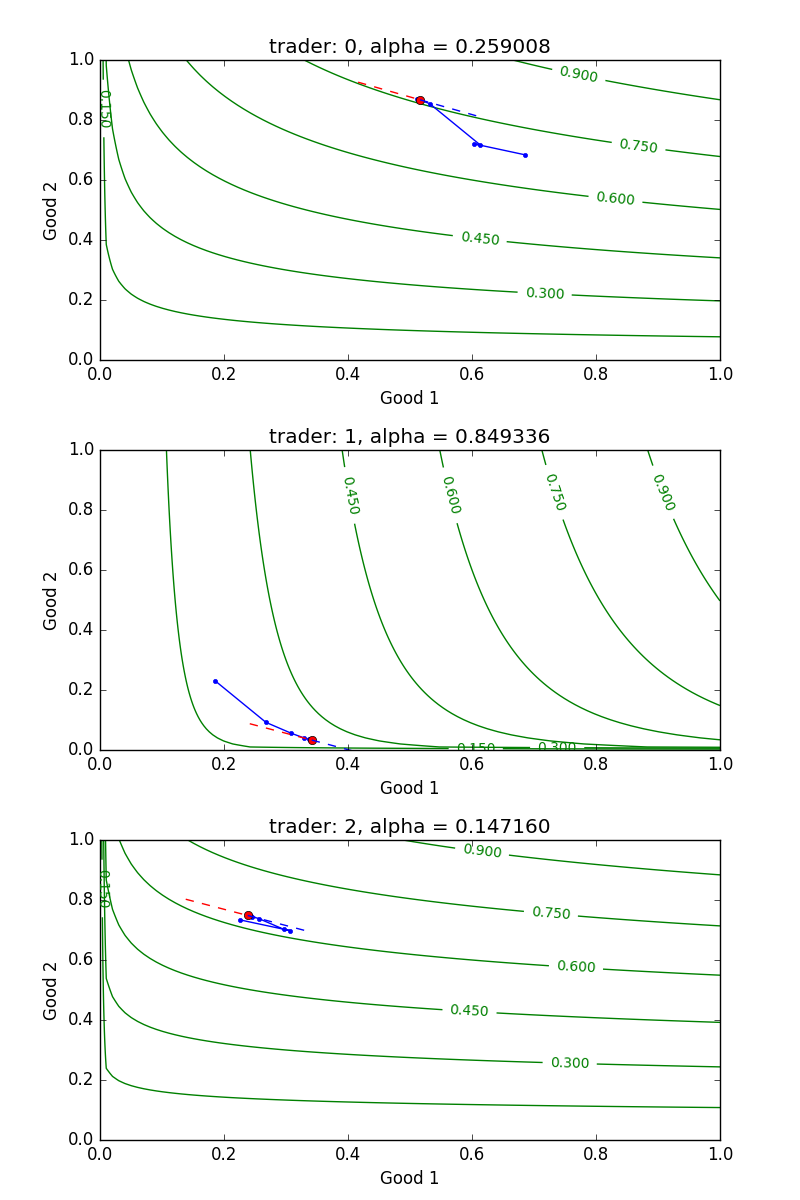
\includegraphics[width=\textwidth]{allocations_(seed_13).png}
    \caption{
      A single trading day for three traders.
      The green contours are lines of equal utility.
      Notice how the trades only increase utility.
      The red dots are the final positions of traders.
      The dashed lines are the bounds on the MRS; the red one is selling and the blue one is buying.
      A trader will only trade above those lines.
    }
    \label{fig:day}
\end{figure}

\section{Design and Implementation}\label{desimp}
We created a software framework to implement the algorithm above and test it with different parameters.
The implementation makes it possible to refine the theoretical algorithm to better model the behaviour of participants in a decentralized market.
We chose to develop in Python, because it allowed for rapid prototyping and flexible experimentation.
The program runs multiple trials using the same parameters, where each trial consists of many days of trading.
Here, we discuss the details of the algorithm as implemented, and the concepts that were important to the implementation.
In particular, we discuss the goal of convergence and the challenge of divergence.

\subsection{The Trading Day}

Each day of the simulation begins by giving each trader their initial endowment.
Then, pairs of traders are repeatedly selected at random to attempt a trade.
The day continues until the traders can't trade anymore.

When two traders are selected to trade, each has access to their utility functions and the gradients of those functions.
From the gradient and any constraints, we calculate two MRSs for each trader, one for each direction.
The direction of the potential trade (Trader 1 buying from Trader 2 or vice versa) is chosen based on the differences between their MRSs.
The trader with the higher MRS is the one who buys Good 1.

In the standard model (see Section \ref{nograd} for the version without access to gradients), we calculate a joint MRS by taking the geometric mean of two MRSs.
This joint MRS is the exchange rate used for the potential.
We experimented with randomly picking an MRS between the two traders' MRSs, but this was slower and gave worse results.

Then, we calculate the size of the biggest possible trade that can occur at that MRS.
A trade can occur if, after reallocation, both traders would have higher utilities.
Because we restrict ourselves to using an oracle that only tells us the utility and gradient at specifc allocation, we cannot calculate the maximum size directly.
Instead, we test progressively larger sizes, doubling each time.
Since the gradient only applies to infinitesimally small sizes, when the MRSs are very similar, the minimum size might not be possible.
If the largest size is non-zero, the traders exchange the appropriate goods and the process repeats.
Figure \ref{fig:day} shows a day of trading with three traders.

As we go, we keep track of the most recent MRS each trader agreed to trade at.
We use this later on to assess the quality of the simulation.

The simulation of a day ends once traders can make no more mutually beneficial trades.
To check for this, we track the number of consecutive attempted trades that are rejected. 
For a simulation with $n$ traders, we wait for $n$ consecutive such empty trades.
There is a parameter that can increase or decrease this, but we found in practice that $n$ gives just as good results as $2n$ or $5n$, and is faster.
We do adjust that parameter when we get to the no-gradient case in Section \ref{nograd}.

\begin{figure}[H]
    \centering
    %% Creator: Matplotlib, PGF backend
%%
%% To include the figure in your LaTeX document, write
%%   \input{<filename>.pgf}
%%
%% Make sure the required packages are loaded in your preamble
%%   \usepackage{pgf}
%%
%% Figures using additional raster images can only be included by \input if
%% they are in the same directory as the main LaTeX file. For loading figures
%% from other directories you can use the `import` package
%%   \usepackage{import}
%% and then include the figures with
%%   \import{<path to file>}{<filename>.pgf}
%%
%% Matplotlib used the following preamble
%%   \usepackage[utf8x]{inputenc}
%%   \usepackage[T1]{fontenc}
%%
\begingroup%
\makeatletter%
\begin{pgfpicture}%
\pgfpathrectangle{\pgfpointorigin}{\pgfqpoint{5.882538in}{7.174123in}}%
\pgfusepath{use as bounding box, clip}%
\begin{pgfscope}%
\pgfsetbuttcap%
\pgfsetmiterjoin%
\definecolor{currentfill}{rgb}{1.000000,1.000000,1.000000}%
\pgfsetfillcolor{currentfill}%
\pgfsetlinewidth{0.000000pt}%
\definecolor{currentstroke}{rgb}{1.000000,1.000000,1.000000}%
\pgfsetstrokecolor{currentstroke}%
\pgfsetdash{}{0pt}%
\pgfpathmoveto{\pgfqpoint{0.000000in}{0.000000in}}%
\pgfpathlineto{\pgfqpoint{5.882538in}{0.000000in}}%
\pgfpathlineto{\pgfqpoint{5.882538in}{7.174123in}}%
\pgfpathlineto{\pgfqpoint{0.000000in}{7.174123in}}%
\pgfpathclose%
\pgfusepath{fill}%
\end{pgfscope}%
\begin{pgfscope}%
\pgfsetbuttcap%
\pgfsetmiterjoin%
\definecolor{currentfill}{rgb}{1.000000,1.000000,1.000000}%
\pgfsetfillcolor{currentfill}%
\pgfsetlinewidth{0.000000pt}%
\definecolor{currentstroke}{rgb}{0.000000,0.000000,0.000000}%
\pgfsetstrokecolor{currentstroke}%
\pgfsetstrokeopacity{0.000000}%
\pgfsetdash{}{0pt}%
\pgfpathmoveto{\pgfqpoint{0.549656in}{3.090884in}}%
\pgfpathlineto{\pgfqpoint{5.693803in}{3.090884in}}%
\pgfpathlineto{\pgfqpoint{5.693803in}{6.866946in}}%
\pgfpathlineto{\pgfqpoint{0.549656in}{6.866946in}}%
\pgfpathclose%
\pgfusepath{fill}%
\end{pgfscope}%
\begin{pgfscope}%
\pgfpathrectangle{\pgfqpoint{0.549656in}{3.090884in}}{\pgfqpoint{5.144147in}{3.776062in}} %
\pgfusepath{clip}%
\pgfsetbuttcap%
\pgfsetroundjoin%
\pgfsetlinewidth{1.003750pt}%
\definecolor{currentstroke}{rgb}{0.000000,0.500000,0.000000}%
\pgfsetstrokecolor{currentstroke}%
\pgfsetdash{}{0pt}%
\pgfpathmoveto{\pgfqpoint{0.575281in}{6.866946in}}%
\pgfpathlineto{\pgfqpoint{0.575474in}{6.828804in}}%
\pgfpathlineto{\pgfqpoint{0.575671in}{6.790662in}}%
\pgfpathlineto{\pgfqpoint{0.575871in}{6.752520in}}%
\pgfpathlineto{\pgfqpoint{0.576076in}{6.714378in}}%
\pgfpathlineto{\pgfqpoint{0.576284in}{6.676236in}}%
\pgfpathlineto{\pgfqpoint{0.576496in}{6.638094in}}%
\pgfpathlineto{\pgfqpoint{0.576545in}{6.629326in}}%
\pgfusepath{stroke}%
\end{pgfscope}%
\begin{pgfscope}%
\pgfpathrectangle{\pgfqpoint{0.549656in}{3.090884in}}{\pgfqpoint{5.144147in}{3.776062in}} %
\pgfusepath{clip}%
\pgfsetbuttcap%
\pgfsetroundjoin%
\pgfsetlinewidth{1.003750pt}%
\definecolor{currentstroke}{rgb}{0.000000,0.500000,0.000000}%
\pgfsetstrokecolor{currentstroke}%
\pgfsetdash{}{0pt}%
\pgfpathmoveto{\pgfqpoint{0.579327in}{6.189158in}}%
\pgfpathlineto{\pgfqpoint{0.585059in}{5.531975in}}%
\pgfpathlineto{\pgfqpoint{0.591546in}{5.036128in}}%
\pgfpathlineto{\pgfqpoint{0.598028in}{4.692850in}}%
\pgfpathlineto{\pgfqpoint{0.602299in}{4.540282in}}%
\pgfpathlineto{\pgfqpoint{0.618944in}{4.425855in}}%
\pgfpathlineto{\pgfqpoint{0.638274in}{4.311429in}}%
\pgfpathlineto{\pgfqpoint{0.653578in}{4.232396in}}%
\pgfpathlineto{\pgfqpoint{0.677309in}{4.158861in}}%
\pgfpathlineto{\pgfqpoint{0.705539in}{4.081550in}}%
\pgfpathlineto{\pgfqpoint{0.724813in}{4.044435in}}%
\pgfpathlineto{\pgfqpoint{0.757500in}{3.986824in}}%
\pgfpathlineto{\pgfqpoint{0.771198in}{3.968151in}}%
\pgfpathlineto{\pgfqpoint{0.809461in}{3.919595in}}%
\pgfpathlineto{\pgfqpoint{0.861422in}{3.868444in}}%
\pgfpathlineto{\pgfqpoint{0.913384in}{3.827657in}}%
\pgfpathlineto{\pgfqpoint{0.965345in}{3.794071in}}%
\pgfpathlineto{\pgfqpoint{1.017306in}{3.765706in}}%
\pgfpathlineto{\pgfqpoint{1.073895in}{3.739299in}}%
\pgfpathlineto{\pgfqpoint{1.121228in}{3.720012in}}%
\pgfpathlineto{\pgfqpoint{1.173189in}{3.701094in}}%
\pgfpathlineto{\pgfqpoint{1.225150in}{3.684336in}}%
\pgfpathlineto{\pgfqpoint{1.299734in}{3.663015in}}%
\pgfpathlineto{\pgfqpoint{1.381033in}{3.642802in}}%
\pgfpathlineto{\pgfqpoint{1.484955in}{3.620496in}}%
\pgfpathlineto{\pgfqpoint{1.588878in}{3.601397in}}%
\pgfpathlineto{\pgfqpoint{1.692800in}{3.584606in}}%
\pgfpathlineto{\pgfqpoint{1.796722in}{3.569894in}}%
\pgfpathlineto{\pgfqpoint{1.952605in}{3.550499in}}%
\pgfpathlineto{\pgfqpoint{2.056527in}{3.539221in}}%
\pgfpathlineto{\pgfqpoint{2.212411in}{3.524079in}}%
\pgfpathlineto{\pgfqpoint{2.420255in}{3.506555in}}%
\pgfpathlineto{\pgfqpoint{2.628099in}{3.491601in}}%
\pgfpathlineto{\pgfqpoint{2.887905in}{3.475360in}}%
\pgfpathlineto{\pgfqpoint{3.147710in}{3.461530in}}%
\pgfpathlineto{\pgfqpoint{3.459476in}{3.447151in}}%
\pgfpathlineto{\pgfqpoint{3.823204in}{3.432690in}}%
\pgfpathlineto{\pgfqpoint{4.238893in}{3.418820in}}%
\pgfpathlineto{\pgfqpoint{4.706542in}{3.405396in}}%
\pgfpathlineto{\pgfqpoint{5.226153in}{3.392659in}}%
\pgfpathlineto{\pgfqpoint{5.693803in}{3.382868in}}%
\pgfpathlineto{\pgfqpoint{5.693803in}{3.382868in}}%
\pgfusepath{stroke}%
\end{pgfscope}%
\begin{pgfscope}%
\pgfpathrectangle{\pgfqpoint{0.549656in}{3.090884in}}{\pgfqpoint{5.144147in}{3.776062in}} %
\pgfusepath{clip}%
\pgfsetbuttcap%
\pgfsetroundjoin%
\pgfsetlinewidth{1.003750pt}%
\definecolor{currentstroke}{rgb}{0.000000,0.500000,0.000000}%
\pgfsetstrokecolor{currentstroke}%
\pgfsetdash{}{0pt}%
\pgfpathmoveto{\pgfqpoint{0.600905in}{6.866946in}}%
\pgfpathlineto{\pgfqpoint{0.601967in}{6.790662in}}%
\pgfpathlineto{\pgfqpoint{0.619392in}{6.485526in}}%
\pgfpathlineto{\pgfqpoint{0.637039in}{6.218531in}}%
\pgfpathlineto{\pgfqpoint{0.653578in}{5.999800in}}%
\pgfpathlineto{\pgfqpoint{0.674021in}{5.837111in}}%
\pgfpathlineto{\pgfqpoint{0.695207in}{5.684543in}}%
\pgfpathlineto{\pgfqpoint{0.706950in}{5.608259in}}%
\pgfpathlineto{\pgfqpoint{0.730557in}{5.493833in}}%
\pgfpathlineto{\pgfqpoint{0.757500in}{5.373896in}}%
\pgfpathlineto{\pgfqpoint{0.789710in}{5.264980in}}%
\pgfpathlineto{\pgfqpoint{0.814728in}{5.188696in}}%
\pgfpathlineto{\pgfqpoint{0.844777in}{5.112412in}}%
\pgfpathlineto{\pgfqpoint{0.861422in}{5.072210in}}%
\pgfpathlineto{\pgfqpoint{0.898025in}{4.997986in}}%
\pgfpathlineto{\pgfqpoint{0.918315in}{4.959844in}}%
\pgfpathlineto{\pgfqpoint{0.965345in}{4.882661in}}%
\pgfpathlineto{\pgfqpoint{1.019829in}{4.807276in}}%
\pgfpathlineto{\pgfqpoint{1.069267in}{4.748243in}}%
\pgfpathlineto{\pgfqpoint{1.122346in}{4.692850in}}%
\pgfpathlineto{\pgfqpoint{1.173189in}{4.645911in}}%
\pgfpathlineto{\pgfqpoint{1.225150in}{4.603014in}}%
\pgfpathlineto{\pgfqpoint{1.277111in}{4.564349in}}%
\pgfpathlineto{\pgfqpoint{1.329072in}{4.529238in}}%
\pgfpathlineto{\pgfqpoint{1.381033in}{4.497142in}}%
\pgfpathlineto{\pgfqpoint{1.439842in}{4.463997in}}%
\pgfpathlineto{\pgfqpoint{1.514675in}{4.425855in}}%
\pgfpathlineto{\pgfqpoint{1.536916in}{4.415171in}}%
\pgfpathlineto{\pgfqpoint{1.597974in}{4.387713in}}%
\pgfpathlineto{\pgfqpoint{1.691318in}{4.349571in}}%
\pgfpathlineto{\pgfqpoint{1.744761in}{4.329632in}}%
\pgfpathlineto{\pgfqpoint{1.848683in}{4.294051in}}%
\pgfpathlineto{\pgfqpoint{1.952605in}{4.262112in}}%
\pgfpathlineto{\pgfqpoint{2.056527in}{4.233195in}}%
\pgfpathlineto{\pgfqpoint{2.160449in}{4.206898in}}%
\pgfpathlineto{\pgfqpoint{2.264372in}{4.182782in}}%
\pgfpathlineto{\pgfqpoint{2.376433in}{4.158861in}}%
\pgfpathlineto{\pgfqpoint{2.524177in}{4.130239in}}%
\pgfpathlineto{\pgfqpoint{2.680060in}{4.103010in}}%
\pgfpathlineto{\pgfqpoint{2.835944in}{4.078307in}}%
\pgfpathlineto{\pgfqpoint{2.991827in}{4.055824in}}%
\pgfpathlineto{\pgfqpoint{3.147710in}{4.035175in}}%
\pgfpathlineto{\pgfqpoint{3.355554in}{4.010093in}}%
\pgfpathlineto{\pgfqpoint{3.563399in}{3.987453in}}%
\pgfpathlineto{\pgfqpoint{3.771243in}{3.966750in}}%
\pgfpathlineto{\pgfqpoint{4.031048in}{3.943367in}}%
\pgfpathlineto{\pgfqpoint{4.290854in}{3.922177in}}%
\pgfpathlineto{\pgfqpoint{4.602620in}{3.899240in}}%
\pgfpathlineto{\pgfqpoint{4.694763in}{3.892889in}}%
\pgfpathlineto{\pgfqpoint{4.694763in}{3.892889in}}%
\pgfusepath{stroke}%
\end{pgfscope}%
\begin{pgfscope}%
\pgfpathrectangle{\pgfqpoint{0.549656in}{3.090884in}}{\pgfqpoint{5.144147in}{3.776062in}} %
\pgfusepath{clip}%
\pgfsetbuttcap%
\pgfsetroundjoin%
\pgfsetlinewidth{1.003750pt}%
\definecolor{currentstroke}{rgb}{0.000000,0.500000,0.000000}%
\pgfsetstrokecolor{currentstroke}%
\pgfsetdash{}{0pt}%
\pgfpathmoveto{\pgfqpoint{5.134067in}{3.865185in}}%
\pgfpathlineto{\pgfqpoint{5.174192in}{3.862820in}}%
\pgfpathlineto{\pgfqpoint{5.226153in}{3.859799in}}%
\pgfpathlineto{\pgfqpoint{5.278114in}{3.856821in}}%
\pgfpathlineto{\pgfqpoint{5.330075in}{3.853884in}}%
\pgfpathlineto{\pgfqpoint{5.332915in}{3.853725in}}%
\pgfpathlineto{\pgfqpoint{5.382036in}{3.851021in}}%
\pgfpathlineto{\pgfqpoint{5.433998in}{3.848200in}}%
\pgfpathlineto{\pgfqpoint{5.485959in}{3.845415in}}%
\pgfpathlineto{\pgfqpoint{5.537920in}{3.842668in}}%
\pgfpathlineto{\pgfqpoint{5.589881in}{3.839956in}}%
\pgfpathlineto{\pgfqpoint{5.641842in}{3.837280in}}%
\pgfpathlineto{\pgfqpoint{5.693803in}{3.834637in}}%
\pgfusepath{stroke}%
\end{pgfscope}%
\begin{pgfscope}%
\pgfpathrectangle{\pgfqpoint{0.549656in}{3.090884in}}{\pgfqpoint{5.144147in}{3.776062in}} %
\pgfusepath{clip}%
\pgfsetbuttcap%
\pgfsetroundjoin%
\pgfsetlinewidth{1.003750pt}%
\definecolor{currentstroke}{rgb}{0.000000,0.500000,0.000000}%
\pgfsetstrokecolor{currentstroke}%
\pgfsetdash{}{0pt}%
\pgfpathmoveto{\pgfqpoint{0.786444in}{6.866946in}}%
\pgfpathlineto{\pgfqpoint{0.809461in}{6.740744in}}%
\pgfpathlineto{\pgfqpoint{0.841243in}{6.599952in}}%
\pgfpathlineto{\pgfqpoint{0.861422in}{6.515397in}}%
\pgfpathlineto{\pgfqpoint{0.891534in}{6.409242in}}%
\pgfpathlineto{\pgfqpoint{0.914326in}{6.332957in}}%
\pgfpathlineto{\pgfqpoint{0.954193in}{6.218531in}}%
\pgfpathlineto{\pgfqpoint{0.968316in}{6.180389in}}%
\pgfpathlineto{\pgfqpoint{1.017306in}{6.062870in}}%
\pgfpathlineto{\pgfqpoint{1.069267in}{5.955410in}}%
\pgfpathlineto{\pgfqpoint{1.113449in}{5.875253in}}%
\pgfpathlineto{\pgfqpoint{1.136240in}{5.837111in}}%
\pgfpathlineto{\pgfqpoint{1.173189in}{5.778563in}}%
\pgfpathlineto{\pgfqpoint{1.225150in}{5.704410in}}%
\pgfpathlineto{\pgfqpoint{1.277111in}{5.637574in}}%
\pgfpathlineto{\pgfqpoint{1.335301in}{5.570117in}}%
\pgfpathlineto{\pgfqpoint{1.381033in}{5.521442in}}%
\pgfpathlineto{\pgfqpoint{1.432994in}{5.470481in}}%
\pgfpathlineto{\pgfqpoint{1.491810in}{5.417548in}}%
\pgfpathlineto{\pgfqpoint{1.537316in}{5.379406in}}%
\pgfpathlineto{\pgfqpoint{1.588878in}{5.339057in}}%
\pgfpathlineto{\pgfqpoint{1.640839in}{5.301041in}}%
\pgfpathlineto{\pgfqpoint{1.693425in}{5.264980in}}%
\pgfpathlineto{\pgfqpoint{1.752930in}{5.226838in}}%
\pgfpathlineto{\pgfqpoint{1.816655in}{5.188696in}}%
\pgfpathlineto{\pgfqpoint{1.884907in}{5.150554in}}%
\pgfpathlineto{\pgfqpoint{1.952605in}{5.115175in}}%
\pgfpathlineto{\pgfqpoint{2.037125in}{5.074270in}}%
\pgfpathlineto{\pgfqpoint{2.108488in}{5.041987in}}%
\pgfpathlineto{\pgfqpoint{2.160449in}{5.019764in}}%
\pgfpathlineto{\pgfqpoint{2.264372in}{4.978070in}}%
\pgfpathlineto{\pgfqpoint{2.368294in}{4.939653in}}%
\pgfpathlineto{\pgfqpoint{2.472216in}{4.904090in}}%
\pgfpathlineto{\pgfqpoint{2.576138in}{4.871028in}}%
\pgfpathlineto{\pgfqpoint{2.680060in}{4.840170in}}%
\pgfpathlineto{\pgfqpoint{2.799002in}{4.807276in}}%
\pgfpathlineto{\pgfqpoint{2.939866in}{4.771200in}}%
\pgfpathlineto{\pgfqpoint{3.043788in}{4.746409in}}%
\pgfpathlineto{\pgfqpoint{3.199671in}{4.711699in}}%
\pgfpathlineto{\pgfqpoint{3.355554in}{4.679636in}}%
\pgfpathlineto{\pgfqpoint{3.511438in}{4.649879in}}%
\pgfpathlineto{\pgfqpoint{3.700232in}{4.616566in}}%
\pgfpathlineto{\pgfqpoint{3.875165in}{4.588030in}}%
\pgfpathlineto{\pgfqpoint{4.083009in}{4.556646in}}%
\pgfpathlineto{\pgfqpoint{4.290854in}{4.527650in}}%
\pgfpathlineto{\pgfqpoint{4.436136in}{4.508642in}}%
\pgfpathlineto{\pgfqpoint{4.436136in}{4.508642in}}%
\pgfusepath{stroke}%
\end{pgfscope}%
\begin{pgfscope}%
\pgfpathrectangle{\pgfqpoint{0.549656in}{3.090884in}}{\pgfqpoint{5.144147in}{3.776062in}} %
\pgfusepath{clip}%
\pgfsetbuttcap%
\pgfsetroundjoin%
\pgfsetlinewidth{1.003750pt}%
\definecolor{currentstroke}{rgb}{0.000000,0.500000,0.000000}%
\pgfsetstrokecolor{currentstroke}%
\pgfsetdash{}{0pt}%
\pgfpathmoveto{\pgfqpoint{4.873244in}{4.456797in}}%
\pgfpathlineto{\pgfqpoint{4.914387in}{4.452284in}}%
\pgfpathlineto{\pgfqpoint{4.966348in}{4.446669in}}%
\pgfpathlineto{\pgfqpoint{5.018309in}{4.441137in}}%
\pgfpathlineto{\pgfqpoint{5.070270in}{4.435685in}}%
\pgfpathlineto{\pgfqpoint{5.122231in}{4.430311in}}%
\pgfpathlineto{\pgfqpoint{5.165917in}{4.425855in}}%
\pgfpathlineto{\pgfqpoint{5.174192in}{4.425020in}}%
\pgfpathlineto{\pgfqpoint{5.226153in}{4.419836in}}%
\pgfpathlineto{\pgfqpoint{5.278114in}{4.414723in}}%
\pgfpathlineto{\pgfqpoint{5.330075in}{4.409681in}}%
\pgfpathlineto{\pgfqpoint{5.382036in}{4.404707in}}%
\pgfpathlineto{\pgfqpoint{5.433998in}{4.399801in}}%
\pgfpathlineto{\pgfqpoint{5.485959in}{4.394959in}}%
\pgfpathlineto{\pgfqpoint{5.537920in}{4.390182in}}%
\pgfpathlineto{\pgfqpoint{5.565083in}{4.387713in}}%
\pgfpathlineto{\pgfqpoint{5.589881in}{4.385483in}}%
\pgfpathlineto{\pgfqpoint{5.641842in}{4.380864in}}%
\pgfpathlineto{\pgfqpoint{5.693803in}{4.376303in}}%
\pgfusepath{stroke}%
\end{pgfscope}%
\begin{pgfscope}%
\pgfpathrectangle{\pgfqpoint{0.549656in}{3.090884in}}{\pgfqpoint{5.144147in}{3.776062in}} %
\pgfusepath{clip}%
\pgfsetbuttcap%
\pgfsetroundjoin%
\pgfsetlinewidth{1.003750pt}%
\definecolor{currentstroke}{rgb}{0.000000,0.500000,0.000000}%
\pgfsetstrokecolor{currentstroke}%
\pgfsetdash{}{0pt}%
\pgfpathmoveto{\pgfqpoint{1.265686in}{6.866946in}}%
\pgfpathlineto{\pgfqpoint{1.277111in}{6.845673in}}%
\pgfpathlineto{\pgfqpoint{1.286735in}{6.828804in}}%
\pgfpathlineto{\pgfqpoint{1.308794in}{6.790662in}}%
\pgfpathlineto{\pgfqpoint{1.329072in}{6.756198in}}%
\pgfpathlineto{\pgfqpoint{1.331363in}{6.752520in}}%
\pgfpathlineto{\pgfqpoint{1.355392in}{6.714378in}}%
\pgfpathlineto{\pgfqpoint{1.379865in}{6.676236in}}%
\pgfpathlineto{\pgfqpoint{1.381033in}{6.674436in}}%
\pgfpathlineto{\pgfqpoint{1.405924in}{6.638094in}}%
\pgfpathlineto{\pgfqpoint{1.432531in}{6.599952in}}%
\pgfpathlineto{\pgfqpoint{1.432994in}{6.599294in}}%
\pgfpathlineto{\pgfqpoint{1.460834in}{6.561810in}}%
\pgfpathlineto{\pgfqpoint{1.484955in}{6.529901in}}%
\pgfpathlineto{\pgfqpoint{1.489906in}{6.523668in}}%
\pgfpathlineto{\pgfqpoint{1.520579in}{6.485526in}}%
\pgfpathlineto{\pgfqpoint{1.536916in}{6.465524in}}%
\pgfpathlineto{\pgfqpoint{1.552453in}{6.447384in}}%
\pgfpathlineto{\pgfqpoint{1.585627in}{6.409242in}}%
\pgfpathlineto{\pgfqpoint{1.588878in}{6.405550in}}%
\pgfpathlineto{\pgfqpoint{1.620627in}{6.371099in}}%
\pgfpathlineto{\pgfqpoint{1.640839in}{6.349510in}}%
\pgfpathlineto{\pgfqpoint{1.657030in}{6.332957in}}%
\pgfpathlineto{\pgfqpoint{1.692800in}{6.296939in}}%
\pgfpathlineto{\pgfqpoint{1.695001in}{6.294815in}}%
\pgfpathlineto{\pgfqpoint{1.735018in}{6.256673in}}%
\pgfpathlineto{\pgfqpoint{1.744761in}{6.247517in}}%
\pgfpathlineto{\pgfqpoint{1.776903in}{6.218531in}}%
\pgfpathlineto{\pgfqpoint{1.796722in}{6.200910in}}%
\pgfpathlineto{\pgfqpoint{1.820743in}{6.180389in}}%
\pgfpathlineto{\pgfqpoint{1.848683in}{6.156847in}}%
\pgfpathlineto{\pgfqpoint{1.866697in}{6.142247in}}%
\pgfpathlineto{\pgfqpoint{1.900644in}{6.115100in}}%
\pgfpathlineto{\pgfqpoint{1.914923in}{6.104105in}}%
\pgfpathlineto{\pgfqpoint{1.952605in}{6.075466in}}%
\pgfpathlineto{\pgfqpoint{1.965579in}{6.065963in}}%
\pgfpathlineto{\pgfqpoint{2.004566in}{6.037767in}}%
\pgfpathlineto{\pgfqpoint{2.018823in}{6.027821in}}%
\pgfpathlineto{\pgfqpoint{2.056527in}{6.001843in}}%
\pgfpathlineto{\pgfqpoint{2.074816in}{5.989679in}}%
\pgfpathlineto{\pgfqpoint{2.108488in}{5.967554in}}%
\pgfpathlineto{\pgfqpoint{2.133721in}{5.951537in}}%
\pgfpathlineto{\pgfqpoint{2.160449in}{5.934772in}}%
\pgfpathlineto{\pgfqpoint{2.195704in}{5.913395in}}%
\pgfpathlineto{\pgfqpoint{2.212411in}{5.903383in}}%
\pgfpathlineto{\pgfqpoint{2.260937in}{5.875253in}}%
\pgfpathlineto{\pgfqpoint{2.264372in}{5.873284in}}%
\pgfpathlineto{\pgfqpoint{2.316333in}{5.844409in}}%
\pgfpathlineto{\pgfqpoint{2.329885in}{5.837111in}}%
\pgfpathlineto{\pgfqpoint{2.368294in}{5.816656in}}%
\pgfpathlineto{\pgfqpoint{2.402571in}{5.798969in}}%
\pgfpathlineto{\pgfqpoint{2.420255in}{5.789943in}}%
\pgfpathlineto{\pgfqpoint{2.472216in}{5.764211in}}%
\pgfpathlineto{\pgfqpoint{2.479243in}{5.760827in}}%
\pgfpathlineto{\pgfqpoint{2.524177in}{5.739418in}}%
\pgfpathlineto{\pgfqpoint{2.560374in}{5.722685in}}%
\pgfpathlineto{\pgfqpoint{2.576138in}{5.715473in}}%
\pgfpathlineto{\pgfqpoint{2.628099in}{5.692350in}}%
\pgfpathlineto{\pgfqpoint{2.646128in}{5.684543in}}%
\pgfpathlineto{\pgfqpoint{2.680060in}{5.669998in}}%
\pgfpathlineto{\pgfqpoint{2.732021in}{5.648352in}}%
\pgfpathlineto{\pgfqpoint{2.736821in}{5.646401in}}%
\pgfpathlineto{\pgfqpoint{2.783982in}{5.627418in}}%
\pgfpathlineto{\pgfqpoint{2.832954in}{5.608259in}}%
\pgfpathlineto{\pgfqpoint{2.835944in}{5.607101in}}%
\pgfpathlineto{\pgfqpoint{2.887905in}{5.587429in}}%
\pgfpathlineto{\pgfqpoint{2.934906in}{5.570117in}}%
\pgfpathlineto{\pgfqpoint{2.939866in}{5.568308in}}%
\pgfpathlineto{\pgfqpoint{2.991827in}{5.549769in}}%
\pgfpathlineto{\pgfqpoint{3.043054in}{5.531975in}}%
\pgfpathlineto{\pgfqpoint{3.043788in}{5.531722in}}%
\pgfpathlineto{\pgfqpoint{3.095749in}{5.514212in}}%
\pgfpathlineto{\pgfqpoint{3.147710in}{5.497147in}}%
\pgfpathlineto{\pgfqpoint{3.158016in}{5.493833in}}%
\pgfpathlineto{\pgfqpoint{3.199671in}{5.480560in}}%
\pgfpathlineto{\pgfqpoint{3.251632in}{5.464391in}}%
\pgfpathlineto{\pgfqpoint{3.280216in}{5.455691in}}%
\pgfpathlineto{\pgfqpoint{3.303593in}{5.448639in}}%
\pgfpathlineto{\pgfqpoint{3.355554in}{5.433292in}}%
\pgfpathlineto{\pgfqpoint{3.407515in}{5.418298in}}%
\pgfpathlineto{\pgfqpoint{3.410162in}{5.417548in}}%
\pgfpathlineto{\pgfqpoint{3.459476in}{5.403703in}}%
\pgfpathlineto{\pgfqpoint{3.511438in}{5.389435in}}%
\pgfpathlineto{\pgfqpoint{3.548731in}{5.379406in}}%
\pgfpathlineto{\pgfqpoint{3.563399in}{5.375496in}}%
\pgfpathlineto{\pgfqpoint{3.615360in}{5.361899in}}%
\pgfpathlineto{\pgfqpoint{3.667321in}{5.348589in}}%
\pgfpathlineto{\pgfqpoint{3.696466in}{5.341264in}}%
\pgfpathlineto{\pgfqpoint{3.719282in}{5.335580in}}%
\pgfpathlineto{\pgfqpoint{3.771243in}{5.322868in}}%
\pgfpathlineto{\pgfqpoint{3.823204in}{5.310412in}}%
\pgfpathlineto{\pgfqpoint{3.854177in}{5.303122in}}%
\pgfpathlineto{\pgfqpoint{3.875165in}{5.298224in}}%
\pgfpathlineto{\pgfqpoint{3.927126in}{5.286306in}}%
\pgfpathlineto{\pgfqpoint{3.979087in}{5.274616in}}%
\pgfpathlineto{\pgfqpoint{4.022717in}{5.264980in}}%
\pgfpathlineto{\pgfqpoint{4.031048in}{5.263156in}}%
\pgfpathlineto{\pgfqpoint{4.083009in}{5.251951in}}%
\pgfpathlineto{\pgfqpoint{4.134971in}{5.240952in}}%
\pgfpathlineto{\pgfqpoint{4.186932in}{5.230153in}}%
\pgfpathlineto{\pgfqpoint{4.203126in}{5.226838in}}%
\pgfpathlineto{\pgfqpoint{4.238893in}{5.219579in}}%
\pgfpathlineto{\pgfqpoint{4.290854in}{5.209206in}}%
\pgfpathlineto{\pgfqpoint{4.342815in}{5.199013in}}%
\pgfpathlineto{\pgfqpoint{4.394776in}{5.188994in}}%
\pgfpathlineto{\pgfqpoint{4.396342in}{5.188696in}}%
\pgfpathlineto{\pgfqpoint{4.446737in}{5.179189in}}%
\pgfpathlineto{\pgfqpoint{4.489862in}{5.171188in}}%
\pgfusepath{stroke}%
\end{pgfscope}%
\begin{pgfscope}%
\pgfpathrectangle{\pgfqpoint{0.549656in}{3.090884in}}{\pgfqpoint{5.144147in}{3.776062in}} %
\pgfusepath{clip}%
\pgfsetbuttcap%
\pgfsetroundjoin%
\pgfsetlinewidth{1.003750pt}%
\definecolor{currentstroke}{rgb}{0.000000,0.500000,0.000000}%
\pgfsetstrokecolor{currentstroke}%
\pgfsetdash{}{0pt}%
\pgfpathmoveto{\pgfqpoint{4.923665in}{5.096608in}}%
\pgfpathlineto{\pgfqpoint{4.966348in}{5.089802in}}%
\pgfpathlineto{\pgfqpoint{5.018309in}{5.081639in}}%
\pgfpathlineto{\pgfqpoint{5.065892in}{5.074270in}}%
\pgfpathlineto{\pgfqpoint{5.070270in}{5.073598in}}%
\pgfpathlineto{\pgfqpoint{5.122231in}{5.065708in}}%
\pgfpathlineto{\pgfqpoint{5.174192in}{5.057930in}}%
\pgfpathlineto{\pgfqpoint{5.226153in}{5.050262in}}%
\pgfpathlineto{\pgfqpoint{5.278114in}{5.042700in}}%
\pgfpathlineto{\pgfqpoint{5.323885in}{5.036128in}}%
\pgfpathlineto{\pgfqpoint{5.330075in}{5.035246in}}%
\pgfpathlineto{\pgfqpoint{5.382036in}{5.027927in}}%
\pgfpathlineto{\pgfqpoint{5.433998in}{5.020706in}}%
\pgfpathlineto{\pgfqpoint{5.485959in}{5.013581in}}%
\pgfpathlineto{\pgfqpoint{5.537920in}{5.006550in}}%
\pgfpathlineto{\pgfqpoint{5.589881in}{4.999611in}}%
\pgfpathlineto{\pgfqpoint{5.602179in}{4.997986in}}%
\pgfpathlineto{\pgfqpoint{5.641842in}{4.992788in}}%
\pgfpathlineto{\pgfqpoint{5.693803in}{4.986060in}}%
\pgfusepath{stroke}%
\end{pgfscope}%
\begin{pgfscope}%
\pgfpathrectangle{\pgfqpoint{0.549656in}{3.090884in}}{\pgfqpoint{5.144147in}{3.776062in}} %
\pgfusepath{clip}%
\pgfsetbuttcap%
\pgfsetroundjoin%
\pgfsetlinewidth{1.003750pt}%
\definecolor{currentstroke}{rgb}{0.000000,0.500000,0.000000}%
\pgfsetstrokecolor{currentstroke}%
\pgfsetdash{}{0pt}%
\pgfpathmoveto{\pgfqpoint{2.243902in}{6.866946in}}%
\pgfpathlineto{\pgfqpoint{2.264372in}{6.851031in}}%
\pgfpathlineto{\pgfqpoint{2.293828in}{6.828804in}}%
\pgfpathlineto{\pgfqpoint{2.316333in}{6.811998in}}%
\pgfpathlineto{\pgfqpoint{2.345757in}{6.790662in}}%
\pgfpathlineto{\pgfqpoint{2.368294in}{6.774485in}}%
\pgfpathlineto{\pgfqpoint{2.399790in}{6.752520in}}%
\pgfpathlineto{\pgfqpoint{2.420255in}{6.738390in}}%
\pgfpathlineto{\pgfqpoint{2.456033in}{6.714378in}}%
\pgfpathlineto{\pgfqpoint{2.472216in}{6.703623in}}%
\pgfpathlineto{\pgfqpoint{2.514590in}{6.676236in}}%
\pgfpathlineto{\pgfqpoint{2.524177in}{6.670099in}}%
\pgfpathlineto{\pgfqpoint{2.575568in}{6.638094in}}%
\pgfpathlineto{\pgfqpoint{2.576138in}{6.637742in}}%
\pgfpathlineto{\pgfqpoint{2.628099in}{6.606499in}}%
\pgfpathlineto{\pgfqpoint{2.639281in}{6.599952in}}%
\pgfpathlineto{\pgfqpoint{2.680060in}{6.576291in}}%
\pgfpathlineto{\pgfqpoint{2.705682in}{6.561810in}}%
\pgfpathlineto{\pgfqpoint{2.732021in}{6.547057in}}%
\pgfpathlineto{\pgfqpoint{2.774873in}{6.523668in}}%
\pgfpathlineto{\pgfqpoint{2.783982in}{6.518740in}}%
\pgfpathlineto{\pgfqpoint{2.835944in}{6.491306in}}%
\pgfpathlineto{\pgfqpoint{2.847158in}{6.485526in}}%
\pgfpathlineto{\pgfqpoint{2.887905in}{6.464706in}}%
\pgfpathlineto{\pgfqpoint{2.922660in}{6.447384in}}%
\pgfpathlineto{\pgfqpoint{2.939866in}{6.438882in}}%
\pgfpathlineto{\pgfqpoint{2.991827in}{6.413804in}}%
\pgfpathlineto{\pgfqpoint{3.001495in}{6.409242in}}%
\pgfpathlineto{\pgfqpoint{3.043788in}{6.389449in}}%
\pgfpathlineto{\pgfqpoint{3.083949in}{6.371099in}}%
\pgfpathlineto{\pgfqpoint{3.095749in}{6.365753in}}%
\pgfpathlineto{\pgfqpoint{3.147710in}{6.342713in}}%
\pgfpathlineto{\pgfqpoint{3.170205in}{6.332957in}}%
\pgfpathlineto{\pgfqpoint{3.199671in}{6.320284in}}%
\pgfpathlineto{\pgfqpoint{3.251632in}{6.298431in}}%
\pgfpathlineto{\pgfqpoint{3.260403in}{6.294815in}}%
\pgfpathlineto{\pgfqpoint{3.303593in}{6.277155in}}%
\pgfpathlineto{\pgfqpoint{3.354841in}{6.256673in}}%
\pgfpathlineto{\pgfqpoint{3.355554in}{6.256390in}}%
\pgfpathlineto{\pgfqpoint{3.407515in}{6.236167in}}%
\pgfpathlineto{\pgfqpoint{3.453853in}{6.218531in}}%
\pgfpathlineto{\pgfqpoint{3.459476in}{6.216408in}}%
\pgfpathlineto{\pgfqpoint{3.511438in}{6.197142in}}%
\pgfpathlineto{\pgfqpoint{3.557609in}{6.180389in}}%
\pgfpathlineto{\pgfqpoint{3.563399in}{6.178304in}}%
\pgfpathlineto{\pgfqpoint{3.615360in}{6.159924in}}%
\pgfpathlineto{\pgfqpoint{3.666403in}{6.142247in}}%
\pgfpathlineto{\pgfqpoint{3.667321in}{6.141932in}}%
\pgfpathlineto{\pgfqpoint{3.719282in}{6.124369in}}%
\pgfpathlineto{\pgfqpoint{3.771243in}{6.107166in}}%
\pgfpathlineto{\pgfqpoint{3.780645in}{6.104105in}}%
\pgfpathlineto{\pgfqpoint{3.823204in}{6.090353in}}%
\pgfpathlineto{\pgfqpoint{3.875165in}{6.073884in}}%
\pgfpathlineto{\pgfqpoint{3.900597in}{6.065963in}}%
\pgfpathlineto{\pgfqpoint{3.927126in}{6.057762in}}%
\pgfpathlineto{\pgfqpoint{3.979087in}{6.041975in}}%
\pgfpathlineto{\pgfqpoint{4.026555in}{6.027821in}}%
\pgfpathlineto{\pgfqpoint{4.027156in}{6.027643in}}%
\pgfusepath{stroke}%
\end{pgfscope}%
\begin{pgfscope}%
\pgfpathrectangle{\pgfqpoint{0.549656in}{3.090884in}}{\pgfqpoint{5.144147in}{3.776062in}} %
\pgfusepath{clip}%
\pgfsetbuttcap%
\pgfsetroundjoin%
\pgfsetlinewidth{1.003750pt}%
\definecolor{currentstroke}{rgb}{0.000000,0.500000,0.000000}%
\pgfsetstrokecolor{currentstroke}%
\pgfsetdash{}{0pt}%
\pgfpathmoveto{\pgfqpoint{4.451770in}{5.911738in}}%
\pgfpathlineto{\pgfqpoint{4.498698in}{5.899979in}}%
\pgfpathlineto{\pgfqpoint{4.550659in}{5.887172in}}%
\pgfpathlineto{\pgfqpoint{4.599805in}{5.875253in}}%
\pgfpathlineto{\pgfqpoint{4.602620in}{5.874575in}}%
\pgfpathlineto{\pgfqpoint{4.654581in}{5.862221in}}%
\pgfpathlineto{\pgfqpoint{4.706542in}{5.850063in}}%
\pgfpathlineto{\pgfqpoint{4.758503in}{5.838094in}}%
\pgfpathlineto{\pgfqpoint{4.762827in}{5.837111in}}%
\pgfpathlineto{\pgfqpoint{4.810465in}{5.826349in}}%
\pgfpathlineto{\pgfqpoint{4.862426in}{5.814787in}}%
\pgfpathlineto{\pgfqpoint{4.914387in}{5.803398in}}%
\pgfpathlineto{\pgfqpoint{4.934863in}{5.798969in}}%
\pgfpathlineto{\pgfqpoint{4.966348in}{5.792204in}}%
\pgfpathlineto{\pgfqpoint{5.018309in}{5.781190in}}%
\pgfpathlineto{\pgfqpoint{5.070270in}{5.770336in}}%
\pgfpathlineto{\pgfqpoint{5.116442in}{5.760827in}}%
\pgfpathlineto{\pgfqpoint{5.122231in}{5.759642in}}%
\pgfpathlineto{\pgfqpoint{5.174192in}{5.749135in}}%
\pgfpathlineto{\pgfqpoint{5.226153in}{5.738776in}}%
\pgfpathlineto{\pgfqpoint{5.278114in}{5.728561in}}%
\pgfpathlineto{\pgfqpoint{5.308382in}{5.722685in}}%
\pgfpathlineto{\pgfqpoint{5.330075in}{5.718501in}}%
\pgfpathlineto{\pgfqpoint{5.382036in}{5.708600in}}%
\pgfpathlineto{\pgfqpoint{5.433998in}{5.698832in}}%
\pgfpathlineto{\pgfqpoint{5.485959in}{5.689195in}}%
\pgfpathlineto{\pgfqpoint{5.511338in}{5.684543in}}%
\pgfpathlineto{\pgfqpoint{5.537920in}{5.679702in}}%
\pgfpathlineto{\pgfqpoint{5.589881in}{5.670351in}}%
\pgfpathlineto{\pgfqpoint{5.641842in}{5.661120in}}%
\pgfpathlineto{\pgfqpoint{5.693803in}{5.652007in}}%
\pgfusepath{stroke}%
\end{pgfscope}%
\begin{pgfscope}%
\pgfpathrectangle{\pgfqpoint{0.549656in}{3.090884in}}{\pgfqpoint{5.144147in}{3.776062in}} %
\pgfusepath{clip}%
\pgfsetbuttcap%
\pgfsetroundjoin%
\pgfsetlinewidth{1.003750pt}%
\definecolor{currentstroke}{rgb}{0.000000,0.500000,0.000000}%
\pgfsetstrokecolor{currentstroke}%
\pgfsetdash{}{0pt}%
\pgfpathmoveto{\pgfqpoint{3.974590in}{6.866946in}}%
\pgfpathlineto{\pgfqpoint{3.979087in}{6.865208in}}%
\pgfpathlineto{\pgfqpoint{4.031048in}{6.845431in}}%
\pgfpathlineto{\pgfqpoint{4.075536in}{6.828804in}}%
\pgfpathlineto{\pgfqpoint{4.083009in}{6.826029in}}%
\pgfpathlineto{\pgfqpoint{4.134971in}{6.807027in}}%
\pgfpathlineto{\pgfqpoint{4.180522in}{6.790662in}}%
\pgfpathlineto{\pgfqpoint{4.186549in}{6.788510in}}%
\pgfusepath{stroke}%
\end{pgfscope}%
\begin{pgfscope}%
\pgfpathrectangle{\pgfqpoint{0.549656in}{3.090884in}}{\pgfqpoint{5.144147in}{3.776062in}} %
\pgfusepath{clip}%
\pgfsetbuttcap%
\pgfsetroundjoin%
\pgfsetlinewidth{1.003750pt}%
\definecolor{currentstroke}{rgb}{0.000000,0.500000,0.000000}%
\pgfsetstrokecolor{currentstroke}%
\pgfsetdash{}{0pt}%
\pgfpathmoveto{\pgfqpoint{4.604514in}{6.650559in}}%
\pgfpathlineto{\pgfqpoint{4.645396in}{6.638094in}}%
\pgfpathlineto{\pgfqpoint{4.654581in}{6.635310in}}%
\pgfpathlineto{\pgfqpoint{4.706542in}{6.619770in}}%
\pgfpathlineto{\pgfqpoint{4.758503in}{6.604472in}}%
\pgfpathlineto{\pgfqpoint{4.774064in}{6.599952in}}%
\pgfpathlineto{\pgfqpoint{4.810465in}{6.589440in}}%
\pgfpathlineto{\pgfqpoint{4.862426in}{6.574650in}}%
\pgfpathlineto{\pgfqpoint{4.908207in}{6.561810in}}%
\pgfpathlineto{\pgfqpoint{4.914387in}{6.560087in}}%
\pgfpathlineto{\pgfqpoint{4.966348in}{6.545776in}}%
\pgfpathlineto{\pgfqpoint{5.018309in}{6.531676in}}%
\pgfpathlineto{\pgfqpoint{5.048220in}{6.523668in}}%
\pgfpathlineto{\pgfqpoint{5.070270in}{6.517798in}}%
\pgfpathlineto{\pgfqpoint{5.122231in}{6.504142in}}%
\pgfpathlineto{\pgfqpoint{5.174192in}{6.490680in}}%
\pgfpathlineto{\pgfqpoint{5.194337in}{6.485526in}}%
\pgfpathlineto{\pgfqpoint{5.226153in}{6.477431in}}%
\pgfpathlineto{\pgfqpoint{5.278114in}{6.464381in}}%
\pgfpathlineto{\pgfqpoint{5.330075in}{6.451510in}}%
\pgfpathlineto{\pgfqpoint{5.346930in}{6.447384in}}%
\pgfpathlineto{\pgfqpoint{5.382036in}{6.438839in}}%
\pgfpathlineto{\pgfqpoint{5.433998in}{6.426350in}}%
\pgfpathlineto{\pgfqpoint{5.485959in}{6.414027in}}%
\pgfpathlineto{\pgfqpoint{5.506376in}{6.409242in}}%
\pgfpathlineto{\pgfqpoint{5.537920in}{6.401889in}}%
\pgfpathlineto{\pgfqpoint{5.589881in}{6.389923in}}%
\pgfpathlineto{\pgfqpoint{5.641842in}{6.378111in}}%
\pgfpathlineto{\pgfqpoint{5.673053in}{6.371099in}}%
\pgfpathlineto{\pgfqpoint{5.693803in}{6.366464in}}%
\pgfusepath{stroke}%
\end{pgfscope}%
\begin{pgfscope}%
\pgfpathrectangle{\pgfqpoint{0.549656in}{3.090884in}}{\pgfqpoint{5.144147in}{3.776062in}} %
\pgfusepath{clip}%
\pgfsetrectcap%
\pgfsetroundjoin%
\pgfsetlinewidth{1.003750pt}%
\definecolor{currentstroke}{rgb}{0.000000,0.000000,1.000000}%
\pgfsetstrokecolor{currentstroke}%
\pgfsetdash{}{0pt}%
\pgfpathmoveto{\pgfqpoint{4.074724in}{5.674020in}}%
\pgfpathlineto{\pgfqpoint{3.547963in}{5.845330in}}%
\pgfpathlineto{\pgfqpoint{3.679653in}{5.806821in}}%
\pgfpathlineto{\pgfqpoint{3.152893in}{6.464337in}}%
\pgfpathlineto{\pgfqpoint{3.119970in}{6.480317in}}%
\pgfusepath{stroke}%
\end{pgfscope}%
\begin{pgfscope}%
\pgfpathrectangle{\pgfqpoint{0.549656in}{3.090884in}}{\pgfqpoint{5.144147in}{3.776062in}} %
\pgfusepath{clip}%
\pgfsetbuttcap%
\pgfsetroundjoin%
\definecolor{currentfill}{rgb}{0.000000,0.000000,1.000000}%
\pgfsetfillcolor{currentfill}%
\pgfsetlinewidth{0.501875pt}%
\definecolor{currentstroke}{rgb}{0.000000,0.000000,1.000000}%
\pgfsetstrokecolor{currentstroke}%
\pgfsetdash{}{0pt}%
\pgfsys@defobject{currentmarker}{\pgfqpoint{-0.020833in}{-0.020833in}}{\pgfqpoint{0.020833in}{0.020833in}}{%
\pgfpathmoveto{\pgfqpoint{0.000000in}{-0.020833in}}%
\pgfpathcurveto{\pgfqpoint{0.005525in}{-0.020833in}}{\pgfqpoint{0.010825in}{-0.018638in}}{\pgfqpoint{0.014731in}{-0.014731in}}%
\pgfpathcurveto{\pgfqpoint{0.018638in}{-0.010825in}}{\pgfqpoint{0.020833in}{-0.005525in}}{\pgfqpoint{0.020833in}{0.000000in}}%
\pgfpathcurveto{\pgfqpoint{0.020833in}{0.005525in}}{\pgfqpoint{0.018638in}{0.010825in}}{\pgfqpoint{0.014731in}{0.014731in}}%
\pgfpathcurveto{\pgfqpoint{0.010825in}{0.018638in}}{\pgfqpoint{0.005525in}{0.020833in}}{\pgfqpoint{0.000000in}{0.020833in}}%
\pgfpathcurveto{\pgfqpoint{-0.005525in}{0.020833in}}{\pgfqpoint{-0.010825in}{0.018638in}}{\pgfqpoint{-0.014731in}{0.014731in}}%
\pgfpathcurveto{\pgfqpoint{-0.018638in}{0.010825in}}{\pgfqpoint{-0.020833in}{0.005525in}}{\pgfqpoint{-0.020833in}{0.000000in}}%
\pgfpathcurveto{\pgfqpoint{-0.020833in}{-0.005525in}}{\pgfqpoint{-0.018638in}{-0.010825in}}{\pgfqpoint{-0.014731in}{-0.014731in}}%
\pgfpathcurveto{\pgfqpoint{-0.010825in}{-0.018638in}}{\pgfqpoint{-0.005525in}{-0.020833in}}{\pgfqpoint{0.000000in}{-0.020833in}}%
\pgfpathclose%
\pgfusepath{stroke,fill}%
}%
\begin{pgfscope}%
\pgfsys@transformshift{4.074724in}{5.674020in}%
\pgfsys@useobject{currentmarker}{}%
\end{pgfscope}%
\begin{pgfscope}%
\pgfsys@transformshift{3.547963in}{5.845330in}%
\pgfsys@useobject{currentmarker}{}%
\end{pgfscope}%
\begin{pgfscope}%
\pgfsys@transformshift{3.679653in}{5.806821in}%
\pgfsys@useobject{currentmarker}{}%
\end{pgfscope}%
\begin{pgfscope}%
\pgfsys@transformshift{3.152893in}{6.464337in}%
\pgfsys@useobject{currentmarker}{}%
\end{pgfscope}%
\begin{pgfscope}%
\pgfsys@transformshift{3.119970in}{6.480317in}%
\pgfsys@useobject{currentmarker}{}%
\end{pgfscope}%
\end{pgfscope}%
\begin{pgfscope}%
\pgfpathrectangle{\pgfqpoint{0.549656in}{3.090884in}}{\pgfqpoint{5.144147in}{3.776062in}} %
\pgfusepath{clip}%
\pgfsetbuttcap%
\pgfsetroundjoin%
\definecolor{currentfill}{rgb}{1.000000,0.000000,0.000000}%
\pgfsetfillcolor{currentfill}%
\pgfsetlinewidth{0.501875pt}%
\definecolor{currentstroke}{rgb}{0.000000,0.000000,0.000000}%
\pgfsetstrokecolor{currentstroke}%
\pgfsetdash{}{0pt}%
\pgfsys@defobject{currentmarker}{\pgfqpoint{-0.041667in}{-0.041667in}}{\pgfqpoint{0.041667in}{0.041667in}}{%
\pgfpathmoveto{\pgfqpoint{0.000000in}{-0.041667in}}%
\pgfpathcurveto{\pgfqpoint{0.011050in}{-0.041667in}}{\pgfqpoint{0.021649in}{-0.037276in}}{\pgfqpoint{0.029463in}{-0.029463in}}%
\pgfpathcurveto{\pgfqpoint{0.037276in}{-0.021649in}}{\pgfqpoint{0.041667in}{-0.011050in}}{\pgfqpoint{0.041667in}{0.000000in}}%
\pgfpathcurveto{\pgfqpoint{0.041667in}{0.011050in}}{\pgfqpoint{0.037276in}{0.021649in}}{\pgfqpoint{0.029463in}{0.029463in}}%
\pgfpathcurveto{\pgfqpoint{0.021649in}{0.037276in}}{\pgfqpoint{0.011050in}{0.041667in}}{\pgfqpoint{0.000000in}{0.041667in}}%
\pgfpathcurveto{\pgfqpoint{-0.011050in}{0.041667in}}{\pgfqpoint{-0.021649in}{0.037276in}}{\pgfqpoint{-0.029463in}{0.029463in}}%
\pgfpathcurveto{\pgfqpoint{-0.037276in}{0.021649in}}{\pgfqpoint{-0.041667in}{0.011050in}}{\pgfqpoint{-0.041667in}{0.000000in}}%
\pgfpathcurveto{\pgfqpoint{-0.041667in}{-0.011050in}}{\pgfqpoint{-0.037276in}{-0.021649in}}{\pgfqpoint{-0.029463in}{-0.029463in}}%
\pgfpathcurveto{\pgfqpoint{-0.021649in}{-0.037276in}}{\pgfqpoint{-0.011050in}{-0.041667in}}{\pgfqpoint{0.000000in}{-0.041667in}}%
\pgfpathclose%
\pgfusepath{stroke,fill}%
}%
\begin{pgfscope}%
\pgfsys@transformshift{3.119970in}{6.480317in}%
\pgfsys@useobject{currentmarker}{}%
\end{pgfscope}%
\end{pgfscope}%
\begin{pgfscope}%
\pgfpathrectangle{\pgfqpoint{0.549656in}{3.090884in}}{\pgfqpoint{5.144147in}{3.776062in}} %
\pgfusepath{clip}%
\pgfsetbuttcap%
\pgfsetroundjoin%
\pgfsetlinewidth{1.003750pt}%
\definecolor{currentstroke}{rgb}{0.000000,0.000000,1.000000}%
\pgfsetstrokecolor{currentstroke}%
\pgfsetdash{{6.000000pt}{6.000000pt}}{0.000000pt}%
\pgfpathmoveto{\pgfqpoint{3.119970in}{6.480317in}}%
\pgfpathlineto{\pgfqpoint{3.248574in}{6.421039in}}%
\pgfpathlineto{\pgfqpoint{3.377177in}{6.361761in}}%
\pgfpathlineto{\pgfqpoint{3.505781in}{6.302483in}}%
\pgfpathlineto{\pgfqpoint{3.634385in}{6.243204in}}%
\pgfusepath{stroke}%
\end{pgfscope}%
\begin{pgfscope}%
\pgfpathrectangle{\pgfqpoint{0.549656in}{3.090884in}}{\pgfqpoint{5.144147in}{3.776062in}} %
\pgfusepath{clip}%
\pgfsetbuttcap%
\pgfsetroundjoin%
\pgfsetlinewidth{1.003750pt}%
\definecolor{currentstroke}{rgb}{1.000000,0.000000,0.000000}%
\pgfsetstrokecolor{currentstroke}%
\pgfsetdash{{6.000000pt}{6.000000pt}}{0.000000pt}%
\pgfpathmoveto{\pgfqpoint{2.605555in}{6.717430in}}%
\pgfpathlineto{\pgfqpoint{2.734159in}{6.658152in}}%
\pgfpathlineto{\pgfqpoint{2.862763in}{6.598874in}}%
\pgfpathlineto{\pgfqpoint{2.991366in}{6.539595in}}%
\pgfpathlineto{\pgfqpoint{3.119970in}{6.480317in}}%
\pgfusepath{stroke}%
\end{pgfscope}%
\begin{pgfscope}%
\pgfsetrectcap%
\pgfsetmiterjoin%
\pgfsetlinewidth{1.003750pt}%
\definecolor{currentstroke}{rgb}{0.000000,0.000000,0.000000}%
\pgfsetstrokecolor{currentstroke}%
\pgfsetdash{}{0pt}%
\pgfpathmoveto{\pgfqpoint{0.549656in}{3.090884in}}%
\pgfpathlineto{\pgfqpoint{0.549656in}{6.866946in}}%
\pgfusepath{stroke}%
\end{pgfscope}%
\begin{pgfscope}%
\pgfsetrectcap%
\pgfsetmiterjoin%
\pgfsetlinewidth{1.003750pt}%
\definecolor{currentstroke}{rgb}{0.000000,0.000000,0.000000}%
\pgfsetstrokecolor{currentstroke}%
\pgfsetdash{}{0pt}%
\pgfpathmoveto{\pgfqpoint{5.693803in}{3.090884in}}%
\pgfpathlineto{\pgfqpoint{5.693803in}{6.866946in}}%
\pgfusepath{stroke}%
\end{pgfscope}%
\begin{pgfscope}%
\pgfsetrectcap%
\pgfsetmiterjoin%
\pgfsetlinewidth{1.003750pt}%
\definecolor{currentstroke}{rgb}{0.000000,0.000000,0.000000}%
\pgfsetstrokecolor{currentstroke}%
\pgfsetdash{}{0pt}%
\pgfpathmoveto{\pgfqpoint{0.549656in}{3.090884in}}%
\pgfpathlineto{\pgfqpoint{5.693803in}{3.090884in}}%
\pgfusepath{stroke}%
\end{pgfscope}%
\begin{pgfscope}%
\pgfsetrectcap%
\pgfsetmiterjoin%
\pgfsetlinewidth{1.003750pt}%
\definecolor{currentstroke}{rgb}{0.000000,0.000000,0.000000}%
\pgfsetstrokecolor{currentstroke}%
\pgfsetdash{}{0pt}%
\pgfpathmoveto{\pgfqpoint{0.549656in}{6.866946in}}%
\pgfpathlineto{\pgfqpoint{5.693803in}{6.866946in}}%
\pgfusepath{stroke}%
\end{pgfscope}%
\begin{pgfscope}%
\pgfsetbuttcap%
\pgfsetroundjoin%
\definecolor{currentfill}{rgb}{0.000000,0.000000,0.000000}%
\pgfsetfillcolor{currentfill}%
\pgfsetlinewidth{0.501875pt}%
\definecolor{currentstroke}{rgb}{0.000000,0.000000,0.000000}%
\pgfsetstrokecolor{currentstroke}%
\pgfsetdash{}{0pt}%
\pgfsys@defobject{currentmarker}{\pgfqpoint{0.000000in}{0.000000in}}{\pgfqpoint{0.000000in}{0.055556in}}{%
\pgfpathmoveto{\pgfqpoint{0.000000in}{0.000000in}}%
\pgfpathlineto{\pgfqpoint{0.000000in}{0.055556in}}%
\pgfusepath{stroke,fill}%
}%
\begin{pgfscope}%
\pgfsys@transformshift{0.549656in}{3.090884in}%
\pgfsys@useobject{currentmarker}{}%
\end{pgfscope}%
\end{pgfscope}%
\begin{pgfscope}%
\pgfsetbuttcap%
\pgfsetroundjoin%
\definecolor{currentfill}{rgb}{0.000000,0.000000,0.000000}%
\pgfsetfillcolor{currentfill}%
\pgfsetlinewidth{0.501875pt}%
\definecolor{currentstroke}{rgb}{0.000000,0.000000,0.000000}%
\pgfsetstrokecolor{currentstroke}%
\pgfsetdash{}{0pt}%
\pgfsys@defobject{currentmarker}{\pgfqpoint{0.000000in}{-0.055556in}}{\pgfqpoint{0.000000in}{0.000000in}}{%
\pgfpathmoveto{\pgfqpoint{0.000000in}{0.000000in}}%
\pgfpathlineto{\pgfqpoint{0.000000in}{-0.055556in}}%
\pgfusepath{stroke,fill}%
}%
\begin{pgfscope}%
\pgfsys@transformshift{0.549656in}{6.866946in}%
\pgfsys@useobject{currentmarker}{}%
\end{pgfscope}%
\end{pgfscope}%
\begin{pgfscope}%
\pgftext[x=0.549656in,y=3.035328in,,top]{\rmfamily\fontsize{10.000000}{12.000000}\selectfont \(\displaystyle 0.0\)}%
\end{pgfscope}%
\begin{pgfscope}%
\pgfsetbuttcap%
\pgfsetroundjoin%
\definecolor{currentfill}{rgb}{0.000000,0.000000,0.000000}%
\pgfsetfillcolor{currentfill}%
\pgfsetlinewidth{0.501875pt}%
\definecolor{currentstroke}{rgb}{0.000000,0.000000,0.000000}%
\pgfsetstrokecolor{currentstroke}%
\pgfsetdash{}{0pt}%
\pgfsys@defobject{currentmarker}{\pgfqpoint{0.000000in}{0.000000in}}{\pgfqpoint{0.000000in}{0.055556in}}{%
\pgfpathmoveto{\pgfqpoint{0.000000in}{0.000000in}}%
\pgfpathlineto{\pgfqpoint{0.000000in}{0.055556in}}%
\pgfusepath{stroke,fill}%
}%
\begin{pgfscope}%
\pgfsys@transformshift{1.578485in}{3.090884in}%
\pgfsys@useobject{currentmarker}{}%
\end{pgfscope}%
\end{pgfscope}%
\begin{pgfscope}%
\pgfsetbuttcap%
\pgfsetroundjoin%
\definecolor{currentfill}{rgb}{0.000000,0.000000,0.000000}%
\pgfsetfillcolor{currentfill}%
\pgfsetlinewidth{0.501875pt}%
\definecolor{currentstroke}{rgb}{0.000000,0.000000,0.000000}%
\pgfsetstrokecolor{currentstroke}%
\pgfsetdash{}{0pt}%
\pgfsys@defobject{currentmarker}{\pgfqpoint{0.000000in}{-0.055556in}}{\pgfqpoint{0.000000in}{0.000000in}}{%
\pgfpathmoveto{\pgfqpoint{0.000000in}{0.000000in}}%
\pgfpathlineto{\pgfqpoint{0.000000in}{-0.055556in}}%
\pgfusepath{stroke,fill}%
}%
\begin{pgfscope}%
\pgfsys@transformshift{1.578485in}{6.866946in}%
\pgfsys@useobject{currentmarker}{}%
\end{pgfscope}%
\end{pgfscope}%
\begin{pgfscope}%
\pgftext[x=1.578485in,y=3.035328in,,top]{\rmfamily\fontsize{10.000000}{12.000000}\selectfont \(\displaystyle 0.2\)}%
\end{pgfscope}%
\begin{pgfscope}%
\pgfsetbuttcap%
\pgfsetroundjoin%
\definecolor{currentfill}{rgb}{0.000000,0.000000,0.000000}%
\pgfsetfillcolor{currentfill}%
\pgfsetlinewidth{0.501875pt}%
\definecolor{currentstroke}{rgb}{0.000000,0.000000,0.000000}%
\pgfsetstrokecolor{currentstroke}%
\pgfsetdash{}{0pt}%
\pgfsys@defobject{currentmarker}{\pgfqpoint{0.000000in}{0.000000in}}{\pgfqpoint{0.000000in}{0.055556in}}{%
\pgfpathmoveto{\pgfqpoint{0.000000in}{0.000000in}}%
\pgfpathlineto{\pgfqpoint{0.000000in}{0.055556in}}%
\pgfusepath{stroke,fill}%
}%
\begin{pgfscope}%
\pgfsys@transformshift{2.607315in}{3.090884in}%
\pgfsys@useobject{currentmarker}{}%
\end{pgfscope}%
\end{pgfscope}%
\begin{pgfscope}%
\pgfsetbuttcap%
\pgfsetroundjoin%
\definecolor{currentfill}{rgb}{0.000000,0.000000,0.000000}%
\pgfsetfillcolor{currentfill}%
\pgfsetlinewidth{0.501875pt}%
\definecolor{currentstroke}{rgb}{0.000000,0.000000,0.000000}%
\pgfsetstrokecolor{currentstroke}%
\pgfsetdash{}{0pt}%
\pgfsys@defobject{currentmarker}{\pgfqpoint{0.000000in}{-0.055556in}}{\pgfqpoint{0.000000in}{0.000000in}}{%
\pgfpathmoveto{\pgfqpoint{0.000000in}{0.000000in}}%
\pgfpathlineto{\pgfqpoint{0.000000in}{-0.055556in}}%
\pgfusepath{stroke,fill}%
}%
\begin{pgfscope}%
\pgfsys@transformshift{2.607315in}{6.866946in}%
\pgfsys@useobject{currentmarker}{}%
\end{pgfscope}%
\end{pgfscope}%
\begin{pgfscope}%
\pgftext[x=2.607315in,y=3.035328in,,top]{\rmfamily\fontsize{10.000000}{12.000000}\selectfont \(\displaystyle 0.4\)}%
\end{pgfscope}%
\begin{pgfscope}%
\pgfsetbuttcap%
\pgfsetroundjoin%
\definecolor{currentfill}{rgb}{0.000000,0.000000,0.000000}%
\pgfsetfillcolor{currentfill}%
\pgfsetlinewidth{0.501875pt}%
\definecolor{currentstroke}{rgb}{0.000000,0.000000,0.000000}%
\pgfsetstrokecolor{currentstroke}%
\pgfsetdash{}{0pt}%
\pgfsys@defobject{currentmarker}{\pgfqpoint{0.000000in}{0.000000in}}{\pgfqpoint{0.000000in}{0.055556in}}{%
\pgfpathmoveto{\pgfqpoint{0.000000in}{0.000000in}}%
\pgfpathlineto{\pgfqpoint{0.000000in}{0.055556in}}%
\pgfusepath{stroke,fill}%
}%
\begin{pgfscope}%
\pgfsys@transformshift{3.636144in}{3.090884in}%
\pgfsys@useobject{currentmarker}{}%
\end{pgfscope}%
\end{pgfscope}%
\begin{pgfscope}%
\pgfsetbuttcap%
\pgfsetroundjoin%
\definecolor{currentfill}{rgb}{0.000000,0.000000,0.000000}%
\pgfsetfillcolor{currentfill}%
\pgfsetlinewidth{0.501875pt}%
\definecolor{currentstroke}{rgb}{0.000000,0.000000,0.000000}%
\pgfsetstrokecolor{currentstroke}%
\pgfsetdash{}{0pt}%
\pgfsys@defobject{currentmarker}{\pgfqpoint{0.000000in}{-0.055556in}}{\pgfqpoint{0.000000in}{0.000000in}}{%
\pgfpathmoveto{\pgfqpoint{0.000000in}{0.000000in}}%
\pgfpathlineto{\pgfqpoint{0.000000in}{-0.055556in}}%
\pgfusepath{stroke,fill}%
}%
\begin{pgfscope}%
\pgfsys@transformshift{3.636144in}{6.866946in}%
\pgfsys@useobject{currentmarker}{}%
\end{pgfscope}%
\end{pgfscope}%
\begin{pgfscope}%
\pgftext[x=3.636144in,y=3.035328in,,top]{\rmfamily\fontsize{10.000000}{12.000000}\selectfont \(\displaystyle 0.6\)}%
\end{pgfscope}%
\begin{pgfscope}%
\pgfsetbuttcap%
\pgfsetroundjoin%
\definecolor{currentfill}{rgb}{0.000000,0.000000,0.000000}%
\pgfsetfillcolor{currentfill}%
\pgfsetlinewidth{0.501875pt}%
\definecolor{currentstroke}{rgb}{0.000000,0.000000,0.000000}%
\pgfsetstrokecolor{currentstroke}%
\pgfsetdash{}{0pt}%
\pgfsys@defobject{currentmarker}{\pgfqpoint{0.000000in}{0.000000in}}{\pgfqpoint{0.000000in}{0.055556in}}{%
\pgfpathmoveto{\pgfqpoint{0.000000in}{0.000000in}}%
\pgfpathlineto{\pgfqpoint{0.000000in}{0.055556in}}%
\pgfusepath{stroke,fill}%
}%
\begin{pgfscope}%
\pgfsys@transformshift{4.664974in}{3.090884in}%
\pgfsys@useobject{currentmarker}{}%
\end{pgfscope}%
\end{pgfscope}%
\begin{pgfscope}%
\pgfsetbuttcap%
\pgfsetroundjoin%
\definecolor{currentfill}{rgb}{0.000000,0.000000,0.000000}%
\pgfsetfillcolor{currentfill}%
\pgfsetlinewidth{0.501875pt}%
\definecolor{currentstroke}{rgb}{0.000000,0.000000,0.000000}%
\pgfsetstrokecolor{currentstroke}%
\pgfsetdash{}{0pt}%
\pgfsys@defobject{currentmarker}{\pgfqpoint{0.000000in}{-0.055556in}}{\pgfqpoint{0.000000in}{0.000000in}}{%
\pgfpathmoveto{\pgfqpoint{0.000000in}{0.000000in}}%
\pgfpathlineto{\pgfqpoint{0.000000in}{-0.055556in}}%
\pgfusepath{stroke,fill}%
}%
\begin{pgfscope}%
\pgfsys@transformshift{4.664974in}{6.866946in}%
\pgfsys@useobject{currentmarker}{}%
\end{pgfscope}%
\end{pgfscope}%
\begin{pgfscope}%
\pgftext[x=4.664974in,y=3.035328in,,top]{\rmfamily\fontsize{10.000000}{12.000000}\selectfont \(\displaystyle 0.8\)}%
\end{pgfscope}%
\begin{pgfscope}%
\pgfsetbuttcap%
\pgfsetroundjoin%
\definecolor{currentfill}{rgb}{0.000000,0.000000,0.000000}%
\pgfsetfillcolor{currentfill}%
\pgfsetlinewidth{0.501875pt}%
\definecolor{currentstroke}{rgb}{0.000000,0.000000,0.000000}%
\pgfsetstrokecolor{currentstroke}%
\pgfsetdash{}{0pt}%
\pgfsys@defobject{currentmarker}{\pgfqpoint{0.000000in}{0.000000in}}{\pgfqpoint{0.000000in}{0.055556in}}{%
\pgfpathmoveto{\pgfqpoint{0.000000in}{0.000000in}}%
\pgfpathlineto{\pgfqpoint{0.000000in}{0.055556in}}%
\pgfusepath{stroke,fill}%
}%
\begin{pgfscope}%
\pgfsys@transformshift{5.693803in}{3.090884in}%
\pgfsys@useobject{currentmarker}{}%
\end{pgfscope}%
\end{pgfscope}%
\begin{pgfscope}%
\pgfsetbuttcap%
\pgfsetroundjoin%
\definecolor{currentfill}{rgb}{0.000000,0.000000,0.000000}%
\pgfsetfillcolor{currentfill}%
\pgfsetlinewidth{0.501875pt}%
\definecolor{currentstroke}{rgb}{0.000000,0.000000,0.000000}%
\pgfsetstrokecolor{currentstroke}%
\pgfsetdash{}{0pt}%
\pgfsys@defobject{currentmarker}{\pgfqpoint{0.000000in}{-0.055556in}}{\pgfqpoint{0.000000in}{0.000000in}}{%
\pgfpathmoveto{\pgfqpoint{0.000000in}{0.000000in}}%
\pgfpathlineto{\pgfqpoint{0.000000in}{-0.055556in}}%
\pgfusepath{stroke,fill}%
}%
\begin{pgfscope}%
\pgfsys@transformshift{5.693803in}{6.866946in}%
\pgfsys@useobject{currentmarker}{}%
\end{pgfscope}%
\end{pgfscope}%
\begin{pgfscope}%
\pgftext[x=5.693803in,y=3.035328in,,top]{\rmfamily\fontsize{10.000000}{12.000000}\selectfont \(\displaystyle 1.0\)}%
\end{pgfscope}%
\begin{pgfscope}%
\pgftext[x=3.121729in,y=2.843229in,,top]{\rmfamily\fontsize{12.000000}{14.400000}\selectfont Good 1}%
\end{pgfscope}%
\begin{pgfscope}%
\pgfsetbuttcap%
\pgfsetroundjoin%
\definecolor{currentfill}{rgb}{0.000000,0.000000,0.000000}%
\pgfsetfillcolor{currentfill}%
\pgfsetlinewidth{0.501875pt}%
\definecolor{currentstroke}{rgb}{0.000000,0.000000,0.000000}%
\pgfsetstrokecolor{currentstroke}%
\pgfsetdash{}{0pt}%
\pgfsys@defobject{currentmarker}{\pgfqpoint{0.000000in}{0.000000in}}{\pgfqpoint{0.055556in}{0.000000in}}{%
\pgfpathmoveto{\pgfqpoint{0.000000in}{0.000000in}}%
\pgfpathlineto{\pgfqpoint{0.055556in}{0.000000in}}%
\pgfusepath{stroke,fill}%
}%
\begin{pgfscope}%
\pgfsys@transformshift{0.549656in}{3.090884in}%
\pgfsys@useobject{currentmarker}{}%
\end{pgfscope}%
\end{pgfscope}%
\begin{pgfscope}%
\pgfsetbuttcap%
\pgfsetroundjoin%
\definecolor{currentfill}{rgb}{0.000000,0.000000,0.000000}%
\pgfsetfillcolor{currentfill}%
\pgfsetlinewidth{0.501875pt}%
\definecolor{currentstroke}{rgb}{0.000000,0.000000,0.000000}%
\pgfsetstrokecolor{currentstroke}%
\pgfsetdash{}{0pt}%
\pgfsys@defobject{currentmarker}{\pgfqpoint{-0.055556in}{0.000000in}}{\pgfqpoint{0.000000in}{0.000000in}}{%
\pgfpathmoveto{\pgfqpoint{0.000000in}{0.000000in}}%
\pgfpathlineto{\pgfqpoint{-0.055556in}{0.000000in}}%
\pgfusepath{stroke,fill}%
}%
\begin{pgfscope}%
\pgfsys@transformshift{5.693803in}{3.090884in}%
\pgfsys@useobject{currentmarker}{}%
\end{pgfscope}%
\end{pgfscope}%
\begin{pgfscope}%
\pgftext[x=0.494100in,y=3.090884in,right,]{\rmfamily\fontsize{10.000000}{12.000000}\selectfont \(\displaystyle 0.0\)}%
\end{pgfscope}%
\begin{pgfscope}%
\pgfsetbuttcap%
\pgfsetroundjoin%
\definecolor{currentfill}{rgb}{0.000000,0.000000,0.000000}%
\pgfsetfillcolor{currentfill}%
\pgfsetlinewidth{0.501875pt}%
\definecolor{currentstroke}{rgb}{0.000000,0.000000,0.000000}%
\pgfsetstrokecolor{currentstroke}%
\pgfsetdash{}{0pt}%
\pgfsys@defobject{currentmarker}{\pgfqpoint{0.000000in}{0.000000in}}{\pgfqpoint{0.055556in}{0.000000in}}{%
\pgfpathmoveto{\pgfqpoint{0.000000in}{0.000000in}}%
\pgfpathlineto{\pgfqpoint{0.055556in}{0.000000in}}%
\pgfusepath{stroke,fill}%
}%
\begin{pgfscope}%
\pgfsys@transformshift{0.549656in}{3.846096in}%
\pgfsys@useobject{currentmarker}{}%
\end{pgfscope}%
\end{pgfscope}%
\begin{pgfscope}%
\pgfsetbuttcap%
\pgfsetroundjoin%
\definecolor{currentfill}{rgb}{0.000000,0.000000,0.000000}%
\pgfsetfillcolor{currentfill}%
\pgfsetlinewidth{0.501875pt}%
\definecolor{currentstroke}{rgb}{0.000000,0.000000,0.000000}%
\pgfsetstrokecolor{currentstroke}%
\pgfsetdash{}{0pt}%
\pgfsys@defobject{currentmarker}{\pgfqpoint{-0.055556in}{0.000000in}}{\pgfqpoint{0.000000in}{0.000000in}}{%
\pgfpathmoveto{\pgfqpoint{0.000000in}{0.000000in}}%
\pgfpathlineto{\pgfqpoint{-0.055556in}{0.000000in}}%
\pgfusepath{stroke,fill}%
}%
\begin{pgfscope}%
\pgfsys@transformshift{5.693803in}{3.846096in}%
\pgfsys@useobject{currentmarker}{}%
\end{pgfscope}%
\end{pgfscope}%
\begin{pgfscope}%
\pgftext[x=0.494100in,y=3.846096in,right,]{\rmfamily\fontsize{10.000000}{12.000000}\selectfont \(\displaystyle 0.2\)}%
\end{pgfscope}%
\begin{pgfscope}%
\pgfsetbuttcap%
\pgfsetroundjoin%
\definecolor{currentfill}{rgb}{0.000000,0.000000,0.000000}%
\pgfsetfillcolor{currentfill}%
\pgfsetlinewidth{0.501875pt}%
\definecolor{currentstroke}{rgb}{0.000000,0.000000,0.000000}%
\pgfsetstrokecolor{currentstroke}%
\pgfsetdash{}{0pt}%
\pgfsys@defobject{currentmarker}{\pgfqpoint{0.000000in}{0.000000in}}{\pgfqpoint{0.055556in}{0.000000in}}{%
\pgfpathmoveto{\pgfqpoint{0.000000in}{0.000000in}}%
\pgfpathlineto{\pgfqpoint{0.055556in}{0.000000in}}%
\pgfusepath{stroke,fill}%
}%
\begin{pgfscope}%
\pgfsys@transformshift{0.549656in}{4.601309in}%
\pgfsys@useobject{currentmarker}{}%
\end{pgfscope}%
\end{pgfscope}%
\begin{pgfscope}%
\pgfsetbuttcap%
\pgfsetroundjoin%
\definecolor{currentfill}{rgb}{0.000000,0.000000,0.000000}%
\pgfsetfillcolor{currentfill}%
\pgfsetlinewidth{0.501875pt}%
\definecolor{currentstroke}{rgb}{0.000000,0.000000,0.000000}%
\pgfsetstrokecolor{currentstroke}%
\pgfsetdash{}{0pt}%
\pgfsys@defobject{currentmarker}{\pgfqpoint{-0.055556in}{0.000000in}}{\pgfqpoint{0.000000in}{0.000000in}}{%
\pgfpathmoveto{\pgfqpoint{0.000000in}{0.000000in}}%
\pgfpathlineto{\pgfqpoint{-0.055556in}{0.000000in}}%
\pgfusepath{stroke,fill}%
}%
\begin{pgfscope}%
\pgfsys@transformshift{5.693803in}{4.601309in}%
\pgfsys@useobject{currentmarker}{}%
\end{pgfscope}%
\end{pgfscope}%
\begin{pgfscope}%
\pgftext[x=0.494100in,y=4.601309in,right,]{\rmfamily\fontsize{10.000000}{12.000000}\selectfont \(\displaystyle 0.4\)}%
\end{pgfscope}%
\begin{pgfscope}%
\pgfsetbuttcap%
\pgfsetroundjoin%
\definecolor{currentfill}{rgb}{0.000000,0.000000,0.000000}%
\pgfsetfillcolor{currentfill}%
\pgfsetlinewidth{0.501875pt}%
\definecolor{currentstroke}{rgb}{0.000000,0.000000,0.000000}%
\pgfsetstrokecolor{currentstroke}%
\pgfsetdash{}{0pt}%
\pgfsys@defobject{currentmarker}{\pgfqpoint{0.000000in}{0.000000in}}{\pgfqpoint{0.055556in}{0.000000in}}{%
\pgfpathmoveto{\pgfqpoint{0.000000in}{0.000000in}}%
\pgfpathlineto{\pgfqpoint{0.055556in}{0.000000in}}%
\pgfusepath{stroke,fill}%
}%
\begin{pgfscope}%
\pgfsys@transformshift{0.549656in}{5.356521in}%
\pgfsys@useobject{currentmarker}{}%
\end{pgfscope}%
\end{pgfscope}%
\begin{pgfscope}%
\pgfsetbuttcap%
\pgfsetroundjoin%
\definecolor{currentfill}{rgb}{0.000000,0.000000,0.000000}%
\pgfsetfillcolor{currentfill}%
\pgfsetlinewidth{0.501875pt}%
\definecolor{currentstroke}{rgb}{0.000000,0.000000,0.000000}%
\pgfsetstrokecolor{currentstroke}%
\pgfsetdash{}{0pt}%
\pgfsys@defobject{currentmarker}{\pgfqpoint{-0.055556in}{0.000000in}}{\pgfqpoint{0.000000in}{0.000000in}}{%
\pgfpathmoveto{\pgfqpoint{0.000000in}{0.000000in}}%
\pgfpathlineto{\pgfqpoint{-0.055556in}{0.000000in}}%
\pgfusepath{stroke,fill}%
}%
\begin{pgfscope}%
\pgfsys@transformshift{5.693803in}{5.356521in}%
\pgfsys@useobject{currentmarker}{}%
\end{pgfscope}%
\end{pgfscope}%
\begin{pgfscope}%
\pgftext[x=0.494100in,y=5.356521in,right,]{\rmfamily\fontsize{10.000000}{12.000000}\selectfont \(\displaystyle 0.6\)}%
\end{pgfscope}%
\begin{pgfscope}%
\pgfsetbuttcap%
\pgfsetroundjoin%
\definecolor{currentfill}{rgb}{0.000000,0.000000,0.000000}%
\pgfsetfillcolor{currentfill}%
\pgfsetlinewidth{0.501875pt}%
\definecolor{currentstroke}{rgb}{0.000000,0.000000,0.000000}%
\pgfsetstrokecolor{currentstroke}%
\pgfsetdash{}{0pt}%
\pgfsys@defobject{currentmarker}{\pgfqpoint{0.000000in}{0.000000in}}{\pgfqpoint{0.055556in}{0.000000in}}{%
\pgfpathmoveto{\pgfqpoint{0.000000in}{0.000000in}}%
\pgfpathlineto{\pgfqpoint{0.055556in}{0.000000in}}%
\pgfusepath{stroke,fill}%
}%
\begin{pgfscope}%
\pgfsys@transformshift{0.549656in}{6.111734in}%
\pgfsys@useobject{currentmarker}{}%
\end{pgfscope}%
\end{pgfscope}%
\begin{pgfscope}%
\pgfsetbuttcap%
\pgfsetroundjoin%
\definecolor{currentfill}{rgb}{0.000000,0.000000,0.000000}%
\pgfsetfillcolor{currentfill}%
\pgfsetlinewidth{0.501875pt}%
\definecolor{currentstroke}{rgb}{0.000000,0.000000,0.000000}%
\pgfsetstrokecolor{currentstroke}%
\pgfsetdash{}{0pt}%
\pgfsys@defobject{currentmarker}{\pgfqpoint{-0.055556in}{0.000000in}}{\pgfqpoint{0.000000in}{0.000000in}}{%
\pgfpathmoveto{\pgfqpoint{0.000000in}{0.000000in}}%
\pgfpathlineto{\pgfqpoint{-0.055556in}{0.000000in}}%
\pgfusepath{stroke,fill}%
}%
\begin{pgfscope}%
\pgfsys@transformshift{5.693803in}{6.111734in}%
\pgfsys@useobject{currentmarker}{}%
\end{pgfscope}%
\end{pgfscope}%
\begin{pgfscope}%
\pgftext[x=0.494100in,y=6.111734in,right,]{\rmfamily\fontsize{10.000000}{12.000000}\selectfont \(\displaystyle 0.8\)}%
\end{pgfscope}%
\begin{pgfscope}%
\pgfsetbuttcap%
\pgfsetroundjoin%
\definecolor{currentfill}{rgb}{0.000000,0.000000,0.000000}%
\pgfsetfillcolor{currentfill}%
\pgfsetlinewidth{0.501875pt}%
\definecolor{currentstroke}{rgb}{0.000000,0.000000,0.000000}%
\pgfsetstrokecolor{currentstroke}%
\pgfsetdash{}{0pt}%
\pgfsys@defobject{currentmarker}{\pgfqpoint{0.000000in}{0.000000in}}{\pgfqpoint{0.055556in}{0.000000in}}{%
\pgfpathmoveto{\pgfqpoint{0.000000in}{0.000000in}}%
\pgfpathlineto{\pgfqpoint{0.055556in}{0.000000in}}%
\pgfusepath{stroke,fill}%
}%
\begin{pgfscope}%
\pgfsys@transformshift{0.549656in}{6.866946in}%
\pgfsys@useobject{currentmarker}{}%
\end{pgfscope}%
\end{pgfscope}%
\begin{pgfscope}%
\pgfsetbuttcap%
\pgfsetroundjoin%
\definecolor{currentfill}{rgb}{0.000000,0.000000,0.000000}%
\pgfsetfillcolor{currentfill}%
\pgfsetlinewidth{0.501875pt}%
\definecolor{currentstroke}{rgb}{0.000000,0.000000,0.000000}%
\pgfsetstrokecolor{currentstroke}%
\pgfsetdash{}{0pt}%
\pgfsys@defobject{currentmarker}{\pgfqpoint{-0.055556in}{0.000000in}}{\pgfqpoint{0.000000in}{0.000000in}}{%
\pgfpathmoveto{\pgfqpoint{0.000000in}{0.000000in}}%
\pgfpathlineto{\pgfqpoint{-0.055556in}{0.000000in}}%
\pgfusepath{stroke,fill}%
}%
\begin{pgfscope}%
\pgfsys@transformshift{5.693803in}{6.866946in}%
\pgfsys@useobject{currentmarker}{}%
\end{pgfscope}%
\end{pgfscope}%
\begin{pgfscope}%
\pgftext[x=0.494100in,y=6.866946in,right,]{\rmfamily\fontsize{10.000000}{12.000000}\selectfont \(\displaystyle 1.0\)}%
\end{pgfscope}%
\begin{pgfscope}%
\pgftext[x=0.247186in,y=4.978915in,,bottom,rotate=90.000000]{\rmfamily\fontsize{12.000000}{14.400000}\selectfont Good 2}%
\end{pgfscope}%
\begin{pgfscope}%
\definecolor{textcolor}{rgb}{0.000000,0.500000,0.000000}%
\pgfsetstrokecolor{textcolor}%
\pgfsetfillcolor{textcolor}%
\pgftext[x=0.542530in,y=6.567162in,left,base,rotate=270.361444]{\color{textcolor}\rmfamily\fontsize{10.000000}{12.000000}\selectfont 0.150}%
\end{pgfscope}%
\begin{pgfscope}%
\definecolor{textcolor}{rgb}{0.000000,0.500000,0.000000}%
\pgfsetstrokecolor{textcolor}%
\pgfsetfillcolor{textcolor}%
\pgftext[x=4.754401in,y=3.854272in,left,base,rotate=356.395401]{\color{textcolor}\rmfamily\fontsize{10.000000}{12.000000}\selectfont 0.300}%
\end{pgfscope}%
\begin{pgfscope}%
\definecolor{textcolor}{rgb}{0.000000,0.500000,0.000000}%
\pgfsetstrokecolor{textcolor}%
\pgfsetfillcolor{textcolor}%
\pgftext[x=4.493499in,y=4.466333in,left,base,rotate=353.239884]{\color{textcolor}\rmfamily\fontsize{10.000000}{12.000000}\selectfont 0.450}%
\end{pgfscope}%
\begin{pgfscope}%
\definecolor{textcolor}{rgb}{0.000000,0.500000,0.000000}%
\pgfsetstrokecolor{textcolor}%
\pgfsetfillcolor{textcolor}%
\pgftext[x=4.544873in,y=5.125560in,left,base,rotate=350.250662]{\color{textcolor}\rmfamily\fontsize{10.000000}{12.000000}\selectfont 0.600}%
\end{pgfscope}%
\begin{pgfscope}%
\definecolor{textcolor}{rgb}{0.000000,0.500000,0.000000}%
\pgfsetstrokecolor{textcolor}%
\pgfsetfillcolor{textcolor}%
\pgftext[x=4.077293in,y=5.976101in,left,base,rotate=344.741806]{\color{textcolor}\rmfamily\fontsize{10.000000}{12.000000}\selectfont 0.750}%
\end{pgfscope}%
\begin{pgfscope}%
\definecolor{textcolor}{rgb}{0.000000,0.500000,0.000000}%
\pgfsetstrokecolor{textcolor}%
\pgfsetfillcolor{textcolor}%
\pgftext[x=4.233842in,y=6.734193in,left,base,rotate=341.741634]{\color{textcolor}\rmfamily\fontsize{10.000000}{12.000000}\selectfont 0.900}%
\end{pgfscope}%
\begin{pgfscope}%
\pgftext[x=3.121729in,y=6.936390in,,base]{\rmfamily\fontsize{14.400000}{17.280000}\selectfont Trader 0, \(\displaystyle \alpha\) = 0.26}%
\end{pgfscope}%
\begin{pgfscope}%
\pgfsetbuttcap%
\pgfsetmiterjoin%
\definecolor{currentfill}{rgb}{1.000000,1.000000,1.000000}%
\pgfsetfillcolor{currentfill}%
\pgfsetlinewidth{0.000000pt}%
\definecolor{currentstroke}{rgb}{0.000000,0.000000,0.000000}%
\pgfsetstrokecolor{currentstroke}%
\pgfsetstrokeopacity{0.000000}%
\pgfsetdash{}{0pt}%
\pgfpathmoveto{\pgfqpoint{0.549656in}{0.494841in}}%
\pgfpathlineto{\pgfqpoint{2.999250in}{0.494841in}}%
\pgfpathlineto{\pgfqpoint{2.999250in}{2.382872in}}%
\pgfpathlineto{\pgfqpoint{0.549656in}{2.382872in}}%
\pgfpathclose%
\pgfusepath{fill}%
\end{pgfscope}%
\begin{pgfscope}%
\pgfpathrectangle{\pgfqpoint{0.549656in}{0.494841in}}{\pgfqpoint{2.449594in}{1.888031in}} %
\pgfusepath{clip}%
\pgfsetbuttcap%
\pgfsetroundjoin%
\pgfsetlinewidth{1.003750pt}%
\definecolor{currentstroke}{rgb}{0.000000,0.500000,0.000000}%
\pgfsetstrokecolor{currentstroke}%
\pgfsetdash{}{0pt}%
\pgfpathmoveto{\pgfqpoint{0.812139in}{2.382872in}}%
\pgfpathlineto{\pgfqpoint{0.822210in}{2.020523in}}%
\pgfpathlineto{\pgfqpoint{0.832473in}{1.734458in}}%
\pgfpathlineto{\pgfqpoint{0.842880in}{1.505605in}}%
\pgfpathlineto{\pgfqpoint{0.852728in}{1.333966in}}%
\pgfpathlineto{\pgfqpoint{0.863713in}{1.181398in}}%
\pgfpathlineto{\pgfqpoint{0.874018in}{1.066972in}}%
\pgfpathlineto{\pgfqpoint{0.884700in}{0.971617in}}%
\pgfpathlineto{\pgfqpoint{0.896063in}{0.889750in}}%
\pgfpathlineto{\pgfqpoint{0.904797in}{0.838120in}}%
\pgfpathlineto{\pgfqpoint{0.916459in}{0.780907in}}%
\pgfpathlineto{\pgfqpoint{0.925890in}{0.742765in}}%
\pgfpathlineto{\pgfqpoint{0.937213in}{0.704623in}}%
\pgfpathlineto{\pgfqpoint{0.951249in}{0.666481in}}%
\pgfpathlineto{\pgfqpoint{0.959735in}{0.647410in}}%
\pgfpathlineto{\pgfqpoint{0.970293in}{0.627069in}}%
\pgfpathlineto{\pgfqpoint{0.981203in}{0.609268in}}%
\pgfpathlineto{\pgfqpoint{0.995362in}{0.590196in}}%
\pgfpathlineto{\pgfqpoint{1.019780in}{0.565903in}}%
\pgfpathlineto{\pgfqpoint{1.037654in}{0.552054in}}%
\pgfpathlineto{\pgfqpoint{1.074040in}{0.532983in}}%
\pgfpathlineto{\pgfqpoint{1.118754in}{0.520067in}}%
\pgfpathlineto{\pgfqpoint{1.143497in}{0.513889in}}%
\pgfpathlineto{\pgfqpoint{1.341444in}{0.509760in}}%
\pgfpathlineto{\pgfqpoint{1.638364in}{0.506224in}}%
\pgfpathlineto{\pgfqpoint{2.108488in}{0.503233in}}%
\pgfpathlineto{\pgfqpoint{2.160579in}{0.503002in}}%
\pgfpathlineto{\pgfqpoint{2.160579in}{0.503002in}}%
\pgfusepath{stroke}%
\end{pgfscope}%
\begin{pgfscope}%
\pgfpathrectangle{\pgfqpoint{0.549656in}{0.494841in}}{\pgfqpoint{2.449594in}{1.888031in}} %
\pgfusepath{clip}%
\pgfsetbuttcap%
\pgfsetroundjoin%
\pgfsetlinewidth{1.003750pt}%
\definecolor{currentstroke}{rgb}{0.000000,0.500000,0.000000}%
\pgfsetstrokecolor{currentstroke}%
\pgfsetdash{}{0pt}%
\pgfpathmoveto{\pgfqpoint{2.600753in}{0.501488in}}%
\pgfpathlineto{\pgfqpoint{2.603356in}{0.501481in}}%
\pgfpathlineto{\pgfqpoint{2.628099in}{0.501414in}}%
\pgfpathlineto{\pgfqpoint{2.652843in}{0.501348in}}%
\pgfpathlineto{\pgfqpoint{2.677586in}{0.501284in}}%
\pgfpathlineto{\pgfqpoint{2.702329in}{0.501221in}}%
\pgfpathlineto{\pgfqpoint{2.727073in}{0.501159in}}%
\pgfpathlineto{\pgfqpoint{2.751816in}{0.501099in}}%
\pgfpathlineto{\pgfqpoint{2.776559in}{0.501040in}}%
\pgfpathlineto{\pgfqpoint{2.801303in}{0.500982in}}%
\pgfpathlineto{\pgfqpoint{2.826046in}{0.500925in}}%
\pgfpathlineto{\pgfqpoint{2.850790in}{0.500870in}}%
\pgfpathlineto{\pgfqpoint{2.875533in}{0.500815in}}%
\pgfpathlineto{\pgfqpoint{2.900276in}{0.500762in}}%
\pgfpathlineto{\pgfqpoint{2.925020in}{0.500709in}}%
\pgfpathlineto{\pgfqpoint{2.949763in}{0.500658in}}%
\pgfpathlineto{\pgfqpoint{2.974506in}{0.500607in}}%
\pgfpathlineto{\pgfqpoint{2.999250in}{0.500558in}}%
\pgfusepath{stroke}%
\end{pgfscope}%
\begin{pgfscope}%
\pgfpathrectangle{\pgfqpoint{0.549656in}{0.494841in}}{\pgfqpoint{2.449594in}{1.888031in}} %
\pgfusepath{clip}%
\pgfsetbuttcap%
\pgfsetroundjoin%
\pgfsetlinewidth{1.003750pt}%
\definecolor{currentstroke}{rgb}{0.000000,0.500000,0.000000}%
\pgfsetstrokecolor{currentstroke}%
\pgfsetdash{}{0pt}%
\pgfpathmoveto{\pgfqpoint{1.171018in}{1.953533in}}%
\pgfpathlineto{\pgfqpoint{1.185793in}{1.772600in}}%
\pgfpathlineto{\pgfqpoint{1.200304in}{1.620032in}}%
\pgfpathlineto{\pgfqpoint{1.215037in}{1.486534in}}%
\pgfpathlineto{\pgfqpoint{1.229676in}{1.372108in}}%
\pgfpathlineto{\pgfqpoint{1.243685in}{1.276753in}}%
\pgfpathlineto{\pgfqpoint{1.259893in}{1.181398in}}%
\pgfpathlineto{\pgfqpoint{1.274888in}{1.105114in}}%
\pgfpathlineto{\pgfqpoint{1.292259in}{1.028830in}}%
\pgfpathlineto{\pgfqpoint{1.307352in}{0.971617in}}%
\pgfpathlineto{\pgfqpoint{1.324729in}{0.914404in}}%
\pgfpathlineto{\pgfqpoint{1.345144in}{0.857191in}}%
\pgfpathlineto{\pgfqpoint{1.366187in}{0.807698in}}%
\pgfpathlineto{\pgfqpoint{1.379216in}{0.780907in}}%
\pgfpathlineto{\pgfqpoint{1.400543in}{0.742765in}}%
\pgfpathlineto{\pgfqpoint{1.426135in}{0.704623in}}%
\pgfpathlineto{\pgfqpoint{1.441068in}{0.685552in}}%
\pgfpathlineto{\pgfqpoint{1.465161in}{0.659156in}}%
\pgfpathlineto{\pgfqpoint{1.489904in}{0.636288in}}%
\pgfpathlineto{\pgfqpoint{1.499300in}{0.628339in}}%
\pgfpathlineto{\pgfqpoint{1.525626in}{0.609268in}}%
\pgfpathlineto{\pgfqpoint{1.564134in}{0.587085in}}%
\pgfpathlineto{\pgfqpoint{1.598407in}{0.571125in}}%
\pgfpathlineto{\pgfqpoint{1.653315in}{0.552054in}}%
\pgfpathlineto{\pgfqpoint{1.712594in}{0.538065in}}%
\pgfpathlineto{\pgfqpoint{1.737338in}{0.532746in}}%
\pgfpathlineto{\pgfqpoint{1.836311in}{0.520122in}}%
\pgfpathlineto{\pgfqpoint{1.890782in}{0.513912in}}%
\pgfpathlineto{\pgfqpoint{2.306435in}{0.510005in}}%
\pgfpathlineto{\pgfqpoint{2.925020in}{0.506577in}}%
\pgfpathlineto{\pgfqpoint{2.999250in}{0.506275in}}%
\pgfpathlineto{\pgfqpoint{2.999250in}{0.506275in}}%
\pgfusepath{stroke}%
\end{pgfscope}%
\begin{pgfscope}%
\pgfpathrectangle{\pgfqpoint{0.549656in}{0.494841in}}{\pgfqpoint{2.449594in}{1.888031in}} %
\pgfusepath{clip}%
\pgfsetbuttcap%
\pgfsetroundjoin%
\pgfsetlinewidth{1.003750pt}%
\definecolor{currentstroke}{rgb}{0.000000,0.500000,0.000000}%
\pgfsetstrokecolor{currentstroke}%
\pgfsetdash{}{0pt}%
\pgfpathmoveto{\pgfqpoint{1.506398in}{2.382872in}}%
\pgfpathlineto{\pgfqpoint{1.508121in}{2.363801in}}%
\pgfpathlineto{\pgfqpoint{1.509865in}{2.344730in}}%
\pgfpathlineto{\pgfqpoint{1.511629in}{2.325659in}}%
\pgfpathlineto{\pgfqpoint{1.513415in}{2.306588in}}%
\pgfpathlineto{\pgfqpoint{1.514647in}{2.293573in}}%
\pgfpathlineto{\pgfqpoint{1.515224in}{2.287517in}}%
\pgfpathlineto{\pgfqpoint{1.517061in}{2.268446in}}%
\pgfpathlineto{\pgfqpoint{1.518921in}{2.249375in}}%
\pgfpathlineto{\pgfqpoint{1.520804in}{2.230304in}}%
\pgfpathlineto{\pgfqpoint{1.522711in}{2.211233in}}%
\pgfpathlineto{\pgfqpoint{1.524642in}{2.192162in}}%
\pgfpathlineto{\pgfqpoint{1.526599in}{2.173091in}}%
\pgfpathlineto{\pgfqpoint{1.528581in}{2.154020in}}%
\pgfpathlineto{\pgfqpoint{1.530590in}{2.134949in}}%
\pgfpathlineto{\pgfqpoint{1.532626in}{2.115878in}}%
\pgfpathlineto{\pgfqpoint{1.534689in}{2.096807in}}%
\pgfpathlineto{\pgfqpoint{1.536781in}{2.077736in}}%
\pgfpathlineto{\pgfqpoint{1.538903in}{2.058665in}}%
\pgfpathlineto{\pgfqpoint{1.539391in}{2.054331in}}%
\pgfpathlineto{\pgfqpoint{1.541060in}{2.039594in}}%
\pgfpathlineto{\pgfqpoint{1.543250in}{2.020523in}}%
\pgfpathlineto{\pgfqpoint{1.545472in}{2.001452in}}%
\pgfpathlineto{\pgfqpoint{1.547727in}{1.982381in}}%
\pgfpathlineto{\pgfqpoint{1.550015in}{1.963310in}}%
\pgfpathlineto{\pgfqpoint{1.551320in}{1.952593in}}%
\pgfusepath{stroke}%
\end{pgfscope}%
\begin{pgfscope}%
\pgfpathrectangle{\pgfqpoint{0.549656in}{0.494841in}}{\pgfqpoint{2.449594in}{1.888031in}} %
\pgfusepath{clip}%
\pgfsetbuttcap%
\pgfsetroundjoin%
\pgfsetlinewidth{1.003750pt}%
\definecolor{currentstroke}{rgb}{0.000000,0.500000,0.000000}%
\pgfsetstrokecolor{currentstroke}%
\pgfsetdash{}{0pt}%
\pgfpathmoveto{\pgfqpoint{1.616361in}{1.517317in}}%
\pgfpathlineto{\pgfqpoint{1.618536in}{1.505605in}}%
\pgfpathlineto{\pgfqpoint{1.622157in}{1.486534in}}%
\pgfpathlineto{\pgfqpoint{1.625859in}{1.467463in}}%
\pgfpathlineto{\pgfqpoint{1.629645in}{1.448392in}}%
\pgfpathlineto{\pgfqpoint{1.633519in}{1.429321in}}%
\pgfpathlineto{\pgfqpoint{1.637486in}{1.410250in}}%
\pgfpathlineto{\pgfqpoint{1.638364in}{1.406115in}}%
\pgfpathlineto{\pgfqpoint{1.641559in}{1.391179in}}%
\pgfpathlineto{\pgfqpoint{1.645737in}{1.372108in}}%
\pgfpathlineto{\pgfqpoint{1.650020in}{1.353037in}}%
\pgfpathlineto{\pgfqpoint{1.654414in}{1.333966in}}%
\pgfpathlineto{\pgfqpoint{1.658925in}{1.314895in}}%
\pgfpathlineto{\pgfqpoint{1.663108in}{1.297674in}}%
\pgfpathlineto{\pgfqpoint{1.663560in}{1.295824in}}%
\pgfpathlineto{\pgfqpoint{1.668338in}{1.276753in}}%
\pgfpathlineto{\pgfqpoint{1.673252in}{1.257682in}}%
\pgfpathlineto{\pgfqpoint{1.678309in}{1.238611in}}%
\pgfpathlineto{\pgfqpoint{1.683518in}{1.219540in}}%
\pgfpathlineto{\pgfqpoint{1.687851in}{1.204136in}}%
\pgfpathlineto{\pgfqpoint{1.688890in}{1.200469in}}%
\pgfpathlineto{\pgfqpoint{1.694447in}{1.181398in}}%
\pgfpathlineto{\pgfqpoint{1.700184in}{1.162327in}}%
\pgfpathlineto{\pgfqpoint{1.706113in}{1.143256in}}%
\pgfpathlineto{\pgfqpoint{1.712246in}{1.124185in}}%
\pgfpathlineto{\pgfqpoint{1.712594in}{1.123135in}}%
\pgfpathlineto{\pgfqpoint{1.718616in}{1.105114in}}%
\pgfpathlineto{\pgfqpoint{1.725221in}{1.086043in}}%
\pgfpathlineto{\pgfqpoint{1.732075in}{1.066972in}}%
\pgfpathlineto{\pgfqpoint{1.737338in}{1.052863in}}%
\pgfpathlineto{\pgfqpoint{1.739204in}{1.047901in}}%
\pgfpathlineto{\pgfqpoint{1.746638in}{1.028830in}}%
\pgfpathlineto{\pgfqpoint{1.754384in}{1.009759in}}%
\pgfpathlineto{\pgfqpoint{1.762081in}{0.991595in}}%
\pgfpathlineto{\pgfqpoint{1.762469in}{0.990688in}}%
\pgfpathlineto{\pgfqpoint{1.770944in}{0.971617in}}%
\pgfpathlineto{\pgfqpoint{1.779819in}{0.952546in}}%
\pgfpathlineto{\pgfqpoint{1.786825in}{0.938174in}}%
\pgfpathlineto{\pgfqpoint{1.789137in}{0.933475in}}%
\pgfpathlineto{\pgfqpoint{1.798955in}{0.914404in}}%
\pgfpathlineto{\pgfqpoint{1.809301in}{0.895333in}}%
\pgfpathlineto{\pgfqpoint{1.811568in}{0.891355in}}%
\pgfpathlineto{\pgfqpoint{1.820256in}{0.876262in}}%
\pgfpathlineto{\pgfqpoint{1.831867in}{0.857191in}}%
\pgfpathlineto{\pgfqpoint{1.836311in}{0.850284in}}%
\pgfpathlineto{\pgfqpoint{1.844226in}{0.838120in}}%
\pgfpathlineto{\pgfqpoint{1.857415in}{0.819049in}}%
\pgfpathlineto{\pgfqpoint{1.861055in}{0.814098in}}%
\pgfpathlineto{\pgfqpoint{1.871559in}{0.799978in}}%
\pgfpathlineto{\pgfqpoint{1.885798in}{0.782114in}}%
\pgfpathlineto{\pgfqpoint{1.886773in}{0.780907in}}%
\pgfpathlineto{\pgfqpoint{1.903244in}{0.761836in}}%
\pgfpathlineto{\pgfqpoint{1.910541in}{0.754002in}}%
\pgfpathlineto{\pgfqpoint{1.921156in}{0.742765in}}%
\pgfpathlineto{\pgfqpoint{1.935285in}{0.728968in}}%
\pgfpathlineto{\pgfqpoint{1.940766in}{0.723694in}}%
\pgfpathlineto{\pgfqpoint{1.960028in}{0.706686in}}%
\pgfpathlineto{\pgfqpoint{1.962402in}{0.704623in}}%
\pgfpathlineto{\pgfqpoint{1.984772in}{0.686890in}}%
\pgfpathlineto{\pgfqpoint{1.986489in}{0.685552in}}%
\pgfpathlineto{\pgfqpoint{2.009515in}{0.669309in}}%
\pgfpathlineto{\pgfqpoint{2.013598in}{0.666481in}}%
\pgfpathlineto{\pgfqpoint{2.034258in}{0.653649in}}%
\pgfpathlineto{\pgfqpoint{2.044510in}{0.647410in}}%
\pgfpathlineto{\pgfqpoint{2.059002in}{0.639592in}}%
\pgfpathlineto{\pgfqpoint{2.080338in}{0.628339in}}%
\pgfpathlineto{\pgfqpoint{2.083745in}{0.626769in}}%
\pgfpathlineto{\pgfqpoint{2.108488in}{0.615578in}}%
\pgfpathlineto{\pgfqpoint{2.122775in}{0.609268in}}%
\pgfpathlineto{\pgfqpoint{2.133232in}{0.605315in}}%
\pgfpathlineto{\pgfqpoint{2.157975in}{0.596159in}}%
\pgfpathlineto{\pgfqpoint{2.174483in}{0.590196in}}%
\pgfpathlineto{\pgfqpoint{2.182718in}{0.587723in}}%
\pgfpathlineto{\pgfqpoint{2.207462in}{0.580434in}}%
\pgfpathlineto{\pgfqpoint{2.232205in}{0.573343in}}%
\pgfpathlineto{\pgfqpoint{2.240089in}{0.571125in}}%
\pgfpathlineto{\pgfqpoint{2.256949in}{0.567350in}}%
\pgfpathlineto{\pgfqpoint{2.281692in}{0.561935in}}%
\pgfpathlineto{\pgfqpoint{2.306435in}{0.556661in}}%
\pgfpathlineto{\pgfqpoint{2.328590in}{0.552054in}}%
\pgfpathlineto{\pgfqpoint{2.331179in}{0.551657in}}%
\pgfpathlineto{\pgfqpoint{2.355922in}{0.547913in}}%
\pgfpathlineto{\pgfqpoint{2.380665in}{0.544263in}}%
\pgfpathlineto{\pgfqpoint{2.405409in}{0.540704in}}%
\pgfpathlineto{\pgfqpoint{2.430152in}{0.537231in}}%
\pgfpathlineto{\pgfqpoint{2.454896in}{0.533841in}}%
\pgfpathlineto{\pgfqpoint{2.461257in}{0.532983in}}%
\pgfpathlineto{\pgfqpoint{2.479639in}{0.531426in}}%
\pgfpathlineto{\pgfqpoint{2.504382in}{0.529373in}}%
\pgfpathlineto{\pgfqpoint{2.529126in}{0.527368in}}%
\pgfpathlineto{\pgfqpoint{2.553869in}{0.525408in}}%
\pgfpathlineto{\pgfqpoint{2.578612in}{0.523493in}}%
\pgfpathlineto{\pgfqpoint{2.603356in}{0.521621in}}%
\pgfpathlineto{\pgfqpoint{2.628099in}{0.519789in}}%
\pgfpathlineto{\pgfqpoint{2.652843in}{0.517998in}}%
\pgfpathlineto{\pgfqpoint{2.677586in}{0.516245in}}%
\pgfpathlineto{\pgfqpoint{2.702329in}{0.514529in}}%
\pgfpathlineto{\pgfqpoint{2.711363in}{0.513912in}}%
\pgfpathlineto{\pgfqpoint{2.727073in}{0.513795in}}%
\pgfpathlineto{\pgfqpoint{2.751816in}{0.513614in}}%
\pgfpathlineto{\pgfqpoint{2.776559in}{0.513437in}}%
\pgfpathlineto{\pgfqpoint{2.801303in}{0.513263in}}%
\pgfpathlineto{\pgfqpoint{2.826046in}{0.513093in}}%
\pgfpathlineto{\pgfqpoint{2.850790in}{0.512926in}}%
\pgfpathlineto{\pgfqpoint{2.875533in}{0.512763in}}%
\pgfpathlineto{\pgfqpoint{2.900276in}{0.512602in}}%
\pgfpathlineto{\pgfqpoint{2.925020in}{0.512445in}}%
\pgfpathlineto{\pgfqpoint{2.949763in}{0.512291in}}%
\pgfpathlineto{\pgfqpoint{2.974506in}{0.512140in}}%
\pgfpathlineto{\pgfqpoint{2.999250in}{0.511991in}}%
\pgfusepath{stroke}%
\end{pgfscope}%
\begin{pgfscope}%
\pgfpathrectangle{\pgfqpoint{0.549656in}{0.494841in}}{\pgfqpoint{2.449594in}{1.888031in}} %
\pgfusepath{clip}%
\pgfsetbuttcap%
\pgfsetroundjoin%
\pgfsetlinewidth{1.003750pt}%
\definecolor{currentstroke}{rgb}{0.000000,0.500000,0.000000}%
\pgfsetstrokecolor{currentstroke}%
\pgfsetdash{}{0pt}%
\pgfpathmoveto{\pgfqpoint{1.954596in}{1.955676in}}%
\pgfpathlineto{\pgfqpoint{1.956549in}{1.944239in}}%
\pgfpathlineto{\pgfqpoint{1.959854in}{1.925168in}}%
\pgfpathlineto{\pgfqpoint{1.960028in}{1.924179in}}%
\pgfpathlineto{\pgfqpoint{1.963220in}{1.906097in}}%
\pgfpathlineto{\pgfqpoint{1.966638in}{1.887026in}}%
\pgfpathlineto{\pgfqpoint{1.970111in}{1.867955in}}%
\pgfpathlineto{\pgfqpoint{1.973640in}{1.848884in}}%
\pgfpathlineto{\pgfqpoint{1.977226in}{1.829813in}}%
\pgfpathlineto{\pgfqpoint{1.980872in}{1.810742in}}%
\pgfpathlineto{\pgfqpoint{1.984579in}{1.791671in}}%
\pgfpathlineto{\pgfqpoint{1.984772in}{1.790695in}}%
\pgfpathlineto{\pgfqpoint{1.988359in}{1.772600in}}%
\pgfpathlineto{\pgfqpoint{1.992204in}{1.753529in}}%
\pgfpathlineto{\pgfqpoint{1.996118in}{1.734458in}}%
\pgfpathlineto{\pgfqpoint{2.000101in}{1.715387in}}%
\pgfpathlineto{\pgfqpoint{2.004157in}{1.696316in}}%
\pgfpathlineto{\pgfqpoint{2.008287in}{1.677245in}}%
\pgfpathlineto{\pgfqpoint{2.009515in}{1.671669in}}%
\pgfpathlineto{\pgfqpoint{2.012502in}{1.658174in}}%
\pgfpathlineto{\pgfqpoint{2.016801in}{1.639103in}}%
\pgfpathlineto{\pgfqpoint{2.021183in}{1.620032in}}%
\pgfpathlineto{\pgfqpoint{2.025651in}{1.600961in}}%
\pgfpathlineto{\pgfqpoint{2.030209in}{1.581890in}}%
\pgfpathlineto{\pgfqpoint{2.034258in}{1.565279in}}%
\pgfpathlineto{\pgfqpoint{2.034861in}{1.562819in}}%
\pgfpathlineto{\pgfqpoint{2.039620in}{1.543747in}}%
\pgfpathlineto{\pgfqpoint{2.044480in}{1.524676in}}%
\pgfpathlineto{\pgfqpoint{2.049445in}{1.505605in}}%
\pgfpathlineto{\pgfqpoint{2.054518in}{1.486534in}}%
\pgfpathlineto{\pgfqpoint{2.059002in}{1.470045in}}%
\pgfpathlineto{\pgfqpoint{2.059707in}{1.467463in}}%
\pgfpathlineto{\pgfqpoint{2.065026in}{1.448392in}}%
\pgfpathlineto{\pgfqpoint{2.070468in}{1.429321in}}%
\pgfpathlineto{\pgfqpoint{2.076040in}{1.410250in}}%
\pgfpathlineto{\pgfqpoint{2.081747in}{1.391179in}}%
\pgfpathlineto{\pgfqpoint{2.083745in}{1.384649in}}%
\pgfpathlineto{\pgfqpoint{2.087605in}{1.372108in}}%
\pgfpathlineto{\pgfqpoint{2.093616in}{1.353037in}}%
\pgfpathlineto{\pgfqpoint{2.099782in}{1.333966in}}%
\pgfpathlineto{\pgfqpoint{2.106113in}{1.314895in}}%
\pgfpathlineto{\pgfqpoint{2.108488in}{1.307912in}}%
\pgfpathlineto{\pgfqpoint{2.112625in}{1.295824in}}%
\pgfpathlineto{\pgfqpoint{2.119323in}{1.276753in}}%
\pgfpathlineto{\pgfqpoint{2.126212in}{1.257682in}}%
\pgfpathlineto{\pgfqpoint{2.133232in}{1.238802in}}%
\pgfpathlineto{\pgfqpoint{2.133303in}{1.238611in}}%
\pgfpathlineto{\pgfqpoint{2.140623in}{1.219540in}}%
\pgfpathlineto{\pgfqpoint{2.148168in}{1.200469in}}%
\pgfpathlineto{\pgfqpoint{2.155951in}{1.181398in}}%
\pgfpathlineto{\pgfqpoint{2.157975in}{1.176580in}}%
\pgfpathlineto{\pgfqpoint{2.164002in}{1.162327in}}%
\pgfpathlineto{\pgfqpoint{2.172326in}{1.143256in}}%
\pgfpathlineto{\pgfqpoint{2.180936in}{1.124185in}}%
\pgfpathlineto{\pgfqpoint{2.182718in}{1.120359in}}%
\pgfpathlineto{\pgfqpoint{2.189869in}{1.105114in}}%
\pgfpathlineto{\pgfqpoint{2.199133in}{1.086043in}}%
\pgfpathlineto{\pgfqpoint{2.207462in}{1.069512in}}%
\pgfpathlineto{\pgfqpoint{2.208751in}{1.066972in}}%
\pgfpathlineto{\pgfqpoint{2.218764in}{1.047901in}}%
\pgfpathlineto{\pgfqpoint{2.229182in}{1.028830in}}%
\pgfpathlineto{\pgfqpoint{2.232205in}{1.023498in}}%
\pgfpathlineto{\pgfqpoint{2.240055in}{1.009759in}}%
\pgfpathlineto{\pgfqpoint{2.251409in}{0.990688in}}%
\pgfpathlineto{\pgfqpoint{2.256949in}{0.981757in}}%
\pgfpathlineto{\pgfqpoint{2.263290in}{0.971617in}}%
\pgfpathlineto{\pgfqpoint{2.275744in}{0.952546in}}%
\pgfpathlineto{\pgfqpoint{2.281692in}{0.943834in}}%
\pgfpathlineto{\pgfqpoint{2.288825in}{0.933475in}}%
\pgfpathlineto{\pgfqpoint{2.302591in}{0.914404in}}%
\pgfpathlineto{\pgfqpoint{2.306435in}{0.909324in}}%
\pgfpathlineto{\pgfqpoint{2.317119in}{0.895333in}}%
\pgfpathlineto{\pgfqpoint{2.331179in}{0.877861in}}%
\pgfpathlineto{\pgfqpoint{2.332478in}{0.876262in}}%
\pgfpathlineto{\pgfqpoint{2.348778in}{0.857191in}}%
\pgfpathlineto{\pgfqpoint{2.355922in}{0.849285in}}%
\pgfpathlineto{\pgfqpoint{2.366117in}{0.838120in}}%
\pgfpathlineto{\pgfqpoint{2.380665in}{0.823095in}}%
\pgfpathlineto{\pgfqpoint{2.384625in}{0.819049in}}%
\pgfpathlineto{\pgfqpoint{2.404463in}{0.799978in}}%
\pgfpathlineto{\pgfqpoint{2.405409in}{0.799124in}}%
\pgfpathlineto{\pgfqpoint{2.425822in}{0.780907in}}%
\pgfpathlineto{\pgfqpoint{2.430152in}{0.777297in}}%
\pgfpathlineto{\pgfqpoint{2.448926in}{0.761836in}}%
\pgfpathlineto{\pgfqpoint{2.454896in}{0.757260in}}%
\pgfpathlineto{\pgfqpoint{2.474058in}{0.742765in}}%
\pgfpathlineto{\pgfqpoint{2.479639in}{0.738854in}}%
\pgfpathlineto{\pgfqpoint{2.501576in}{0.723694in}}%
\pgfpathlineto{\pgfqpoint{2.504382in}{0.721906in}}%
\pgfpathlineto{\pgfqpoint{2.529126in}{0.706364in}}%
\pgfpathlineto{\pgfqpoint{2.531937in}{0.704623in}}%
\pgfpathlineto{\pgfqpoint{2.553869in}{0.692179in}}%
\pgfpathlineto{\pgfqpoint{2.565740in}{0.685552in}}%
\pgfpathlineto{\pgfqpoint{2.578612in}{0.679020in}}%
\pgfpathlineto{\pgfqpoint{2.603356in}{0.666684in}}%
\pgfpathlineto{\pgfqpoint{2.603769in}{0.666481in}}%
\pgfpathlineto{\pgfqpoint{2.628099in}{0.655691in}}%
\pgfpathlineto{\pgfqpoint{2.647142in}{0.647410in}}%
\pgfpathlineto{\pgfqpoint{2.652843in}{0.645203in}}%
\pgfpathlineto{\pgfqpoint{2.677586in}{0.635760in}}%
\pgfpathlineto{\pgfqpoint{2.697418in}{0.628339in}}%
\pgfpathlineto{\pgfqpoint{2.702329in}{0.626727in}}%
\pgfpathlineto{\pgfqpoint{2.727073in}{0.618718in}}%
\pgfpathlineto{\pgfqpoint{2.751816in}{0.610876in}}%
\pgfpathlineto{\pgfqpoint{2.756958in}{0.609268in}}%
\pgfpathlineto{\pgfqpoint{2.776559in}{0.604001in}}%
\pgfpathlineto{\pgfqpoint{2.801303in}{0.597476in}}%
\pgfpathlineto{\pgfqpoint{2.826046in}{0.591082in}}%
\pgfpathlineto{\pgfqpoint{2.829513in}{0.590196in}}%
\pgfpathlineto{\pgfqpoint{2.850790in}{0.585663in}}%
\pgfpathlineto{\pgfqpoint{2.875533in}{0.580487in}}%
\pgfpathlineto{\pgfqpoint{2.900276in}{0.575413in}}%
\pgfpathlineto{\pgfqpoint{2.921567in}{0.571125in}}%
\pgfpathlineto{\pgfqpoint{2.925020in}{0.570570in}}%
\pgfpathlineto{\pgfqpoint{2.949763in}{0.566635in}}%
\pgfpathlineto{\pgfqpoint{2.974506in}{0.562774in}}%
\pgfpathlineto{\pgfqpoint{2.999250in}{0.558986in}}%
\pgfusepath{stroke}%
\end{pgfscope}%
\begin{pgfscope}%
\pgfpathrectangle{\pgfqpoint{0.549656in}{0.494841in}}{\pgfqpoint{2.449594in}{1.888031in}} %
\pgfusepath{clip}%
\pgfsetbuttcap%
\pgfsetroundjoin%
\pgfsetlinewidth{1.003750pt}%
\definecolor{currentstroke}{rgb}{0.000000,0.500000,0.000000}%
\pgfsetstrokecolor{currentstroke}%
\pgfsetdash{}{0pt}%
\pgfpathmoveto{\pgfqpoint{2.375013in}{1.963443in}}%
\pgfpathlineto{\pgfqpoint{2.375042in}{1.963310in}}%
\pgfpathlineto{\pgfqpoint{2.379276in}{1.944239in}}%
\pgfpathlineto{\pgfqpoint{2.380665in}{1.938068in}}%
\pgfpathlineto{\pgfqpoint{2.383581in}{1.925168in}}%
\pgfpathlineto{\pgfqpoint{2.387956in}{1.906097in}}%
\pgfpathlineto{\pgfqpoint{2.392399in}{1.887026in}}%
\pgfpathlineto{\pgfqpoint{2.396913in}{1.867955in}}%
\pgfpathlineto{\pgfqpoint{2.401499in}{1.848884in}}%
\pgfpathlineto{\pgfqpoint{2.405409in}{1.832883in}}%
\pgfpathlineto{\pgfqpoint{2.406162in}{1.829813in}}%
\pgfpathlineto{\pgfqpoint{2.410910in}{1.810742in}}%
\pgfpathlineto{\pgfqpoint{2.415738in}{1.791671in}}%
\pgfpathlineto{\pgfqpoint{2.420649in}{1.772600in}}%
\pgfpathlineto{\pgfqpoint{2.425644in}{1.753529in}}%
\pgfpathlineto{\pgfqpoint{2.430152in}{1.736612in}}%
\pgfpathlineto{\pgfqpoint{2.430729in}{1.734458in}}%
\pgfpathlineto{\pgfqpoint{2.435913in}{1.715387in}}%
\pgfpathlineto{\pgfqpoint{2.441192in}{1.696316in}}%
\pgfpathlineto{\pgfqpoint{2.446567in}{1.677245in}}%
\pgfpathlineto{\pgfqpoint{2.452044in}{1.658174in}}%
\pgfpathlineto{\pgfqpoint{2.454896in}{1.648417in}}%
\pgfpathlineto{\pgfqpoint{2.457630in}{1.639103in}}%
\pgfpathlineto{\pgfqpoint{2.463330in}{1.620032in}}%
\pgfpathlineto{\pgfqpoint{2.469142in}{1.600961in}}%
\pgfpathlineto{\pgfqpoint{2.475071in}{1.581890in}}%
\pgfpathlineto{\pgfqpoint{2.479639in}{1.567480in}}%
\pgfpathlineto{\pgfqpoint{2.481124in}{1.562819in}}%
\pgfpathlineto{\pgfqpoint{2.487311in}{1.543747in}}%
\pgfpathlineto{\pgfqpoint{2.493629in}{1.524676in}}%
\pgfpathlineto{\pgfqpoint{2.500083in}{1.505605in}}%
\pgfpathlineto{\pgfqpoint{2.504382in}{1.493161in}}%
\pgfpathlineto{\pgfqpoint{2.506683in}{1.486534in}}%
\pgfpathlineto{\pgfqpoint{2.513439in}{1.467463in}}%
\pgfpathlineto{\pgfqpoint{2.520350in}{1.448392in}}%
\pgfpathlineto{\pgfqpoint{2.527421in}{1.429321in}}%
\pgfpathlineto{\pgfqpoint{2.529126in}{1.424819in}}%
\pgfpathlineto{\pgfqpoint{2.534671in}{1.410250in}}%
\pgfpathlineto{\pgfqpoint{2.542100in}{1.391179in}}%
\pgfpathlineto{\pgfqpoint{2.549713in}{1.372108in}}%
\pgfpathlineto{\pgfqpoint{2.553869in}{1.361938in}}%
\pgfpathlineto{\pgfqpoint{2.557525in}{1.353037in}}%
\pgfpathlineto{\pgfqpoint{2.565548in}{1.333966in}}%
\pgfpathlineto{\pgfqpoint{2.573784in}{1.314895in}}%
\pgfpathlineto{\pgfqpoint{2.578612in}{1.303993in}}%
\pgfpathlineto{\pgfqpoint{2.582250in}{1.295824in}}%
\pgfpathlineto{\pgfqpoint{2.590960in}{1.276753in}}%
\pgfpathlineto{\pgfqpoint{2.599918in}{1.257682in}}%
\pgfpathlineto{\pgfqpoint{2.603356in}{1.250554in}}%
\pgfpathlineto{\pgfqpoint{2.609148in}{1.238611in}}%
\pgfpathlineto{\pgfqpoint{2.618661in}{1.219540in}}%
\pgfpathlineto{\pgfqpoint{2.628099in}{1.201180in}}%
\pgfpathlineto{\pgfqpoint{2.628467in}{1.200469in}}%
\pgfpathlineto{\pgfqpoint{2.638600in}{1.181398in}}%
\pgfpathlineto{\pgfqpoint{2.649063in}{1.162327in}}%
\pgfpathlineto{\pgfqpoint{2.652843in}{1.155641in}}%
\pgfpathlineto{\pgfqpoint{2.659887in}{1.143256in}}%
\pgfpathlineto{\pgfqpoint{2.671092in}{1.124185in}}%
\pgfpathlineto{\pgfqpoint{2.677586in}{1.113488in}}%
\pgfpathlineto{\pgfqpoint{2.682703in}{1.105114in}}%
\pgfpathlineto{\pgfqpoint{2.694751in}{1.086043in}}%
\pgfpathlineto{\pgfqpoint{2.702329in}{1.074462in}}%
\pgfpathlineto{\pgfqpoint{2.707263in}{1.066972in}}%
\pgfpathlineto{\pgfqpoint{2.720278in}{1.047901in}}%
\pgfpathlineto{\pgfqpoint{2.727073in}{1.038308in}}%
\pgfpathlineto{\pgfqpoint{2.733832in}{1.028830in}}%
\pgfpathlineto{\pgfqpoint{2.747967in}{1.009759in}}%
\pgfpathlineto{\pgfqpoint{2.751816in}{1.004762in}}%
\pgfpathlineto{\pgfqpoint{2.762736in}{0.990688in}}%
\pgfpathlineto{\pgfqpoint{2.776559in}{0.973608in}}%
\pgfpathlineto{\pgfqpoint{2.778183in}{0.971617in}}%
\pgfpathlineto{\pgfqpoint{2.794382in}{0.952546in}}%
\pgfpathlineto{\pgfqpoint{2.801303in}{0.944750in}}%
\pgfpathlineto{\pgfqpoint{2.811394in}{0.933475in}}%
\pgfpathlineto{\pgfqpoint{2.826046in}{0.917843in}}%
\pgfpathlineto{\pgfqpoint{2.829296in}{0.914404in}}%
\pgfpathlineto{\pgfqpoint{2.848186in}{0.895333in}}%
\pgfpathlineto{\pgfqpoint{2.850790in}{0.892828in}}%
\pgfpathlineto{\pgfqpoint{2.868168in}{0.876262in}}%
\pgfpathlineto{\pgfqpoint{2.875533in}{0.869594in}}%
\pgfpathlineto{\pgfqpoint{2.889361in}{0.857191in}}%
\pgfpathlineto{\pgfqpoint{2.900276in}{0.847912in}}%
\pgfpathlineto{\pgfqpoint{2.911909in}{0.838120in}}%
\pgfpathlineto{\pgfqpoint{2.925020in}{0.827685in}}%
\pgfpathlineto{\pgfqpoint{2.935982in}{0.819049in}}%
\pgfpathlineto{\pgfqpoint{2.949763in}{0.808812in}}%
\pgfpathlineto{\pgfqpoint{2.961784in}{0.799978in}}%
\pgfpathlineto{\pgfqpoint{2.974506in}{0.791188in}}%
\pgfpathlineto{\pgfqpoint{2.989557in}{0.780907in}}%
\pgfpathlineto{\pgfqpoint{2.999250in}{0.774704in}}%
\pgfusepath{stroke}%
\end{pgfscope}%
\begin{pgfscope}%
\pgfpathrectangle{\pgfqpoint{0.549656in}{0.494841in}}{\pgfqpoint{2.449594in}{1.888031in}} %
\pgfusepath{clip}%
\pgfsetbuttcap%
\pgfsetroundjoin%
\pgfsetlinewidth{1.003750pt}%
\definecolor{currentstroke}{rgb}{0.000000,0.500000,0.000000}%
\pgfsetstrokecolor{currentstroke}%
\pgfsetdash{}{0pt}%
\pgfpathmoveto{\pgfqpoint{2.807966in}{1.978622in}}%
\pgfpathlineto{\pgfqpoint{2.812120in}{1.963310in}}%
\pgfpathlineto{\pgfqpoint{2.817372in}{1.944239in}}%
\pgfpathlineto{\pgfqpoint{2.822705in}{1.925168in}}%
\pgfpathlineto{\pgfqpoint{2.826046in}{1.913389in}}%
\pgfpathlineto{\pgfqpoint{2.828123in}{1.906097in}}%
\pgfpathlineto{\pgfqpoint{2.833631in}{1.887026in}}%
\pgfpathlineto{\pgfqpoint{2.839227in}{1.867955in}}%
\pgfpathlineto{\pgfqpoint{2.844913in}{1.848884in}}%
\pgfpathlineto{\pgfqpoint{2.850692in}{1.829813in}}%
\pgfpathlineto{\pgfqpoint{2.850790in}{1.829496in}}%
\pgfpathlineto{\pgfqpoint{2.856576in}{1.810742in}}%
\pgfpathlineto{\pgfqpoint{2.862560in}{1.791671in}}%
\pgfpathlineto{\pgfqpoint{2.868645in}{1.772600in}}%
\pgfpathlineto{\pgfqpoint{2.874836in}{1.753529in}}%
\pgfpathlineto{\pgfqpoint{2.875533in}{1.751415in}}%
\pgfpathlineto{\pgfqpoint{2.881145in}{1.734458in}}%
\pgfpathlineto{\pgfqpoint{2.887567in}{1.715387in}}%
\pgfpathlineto{\pgfqpoint{2.894106in}{1.696316in}}%
\pgfpathlineto{\pgfqpoint{2.900276in}{1.678644in}}%
\pgfpathlineto{\pgfqpoint{2.900767in}{1.677245in}}%
\pgfpathlineto{\pgfqpoint{2.907562in}{1.658174in}}%
\pgfpathlineto{\pgfqpoint{2.914487in}{1.639103in}}%
\pgfpathlineto{\pgfqpoint{2.921545in}{1.620032in}}%
\pgfpathlineto{\pgfqpoint{2.925020in}{1.610813in}}%
\pgfpathlineto{\pgfqpoint{2.928749in}{1.600961in}}%
\pgfpathlineto{\pgfqpoint{2.936102in}{1.581890in}}%
\pgfpathlineto{\pgfqpoint{2.943606in}{1.562819in}}%
\pgfpathlineto{\pgfqpoint{2.949763in}{1.547478in}}%
\pgfpathlineto{\pgfqpoint{2.951267in}{1.543747in}}%
\pgfpathlineto{\pgfqpoint{2.959100in}{1.524676in}}%
\pgfpathlineto{\pgfqpoint{2.967102in}{1.505605in}}%
\pgfpathlineto{\pgfqpoint{2.974506in}{1.488334in}}%
\pgfpathlineto{\pgfqpoint{2.975281in}{1.486534in}}%
\pgfpathlineto{\pgfqpoint{2.983655in}{1.467463in}}%
\pgfpathlineto{\pgfqpoint{2.992219in}{1.448392in}}%
\pgfpathlineto{\pgfqpoint{2.999250in}{1.433084in}}%
\pgfusepath{stroke}%
\end{pgfscope}%
\begin{pgfscope}%
\pgfpathrectangle{\pgfqpoint{0.549656in}{0.494841in}}{\pgfqpoint{2.449594in}{1.888031in}} %
\pgfusepath{clip}%
\pgfsetrectcap%
\pgfsetroundjoin%
\pgfsetlinewidth{1.003750pt}%
\definecolor{currentstroke}{rgb}{0.000000,0.000000,1.000000}%
\pgfsetstrokecolor{currentstroke}%
\pgfsetdash{}{0pt}%
\pgfpathmoveto{\pgfqpoint{1.004605in}{0.930143in}}%
\pgfpathlineto{\pgfqpoint{1.255443in}{0.601385in}}%
\pgfpathlineto{\pgfqpoint{1.318153in}{0.569291in}}%
\pgfpathlineto{\pgfqpoint{1.333830in}{0.561301in}}%
\pgfpathlineto{\pgfqpoint{1.365185in}{0.548580in}}%
\pgfpathlineto{\pgfqpoint{1.367145in}{0.547859in}}%
\pgfusepath{stroke}%
\end{pgfscope}%
\begin{pgfscope}%
\pgfpathrectangle{\pgfqpoint{0.549656in}{0.494841in}}{\pgfqpoint{2.449594in}{1.888031in}} %
\pgfusepath{clip}%
\pgfsetbuttcap%
\pgfsetroundjoin%
\definecolor{currentfill}{rgb}{0.000000,0.000000,1.000000}%
\pgfsetfillcolor{currentfill}%
\pgfsetlinewidth{0.501875pt}%
\definecolor{currentstroke}{rgb}{0.000000,0.000000,1.000000}%
\pgfsetstrokecolor{currentstroke}%
\pgfsetdash{}{0pt}%
\pgfsys@defobject{currentmarker}{\pgfqpoint{-0.020833in}{-0.020833in}}{\pgfqpoint{0.020833in}{0.020833in}}{%
\pgfpathmoveto{\pgfqpoint{0.000000in}{-0.020833in}}%
\pgfpathcurveto{\pgfqpoint{0.005525in}{-0.020833in}}{\pgfqpoint{0.010825in}{-0.018638in}}{\pgfqpoint{0.014731in}{-0.014731in}}%
\pgfpathcurveto{\pgfqpoint{0.018638in}{-0.010825in}}{\pgfqpoint{0.020833in}{-0.005525in}}{\pgfqpoint{0.020833in}{0.000000in}}%
\pgfpathcurveto{\pgfqpoint{0.020833in}{0.005525in}}{\pgfqpoint{0.018638in}{0.010825in}}{\pgfqpoint{0.014731in}{0.014731in}}%
\pgfpathcurveto{\pgfqpoint{0.010825in}{0.018638in}}{\pgfqpoint{0.005525in}{0.020833in}}{\pgfqpoint{0.000000in}{0.020833in}}%
\pgfpathcurveto{\pgfqpoint{-0.005525in}{0.020833in}}{\pgfqpoint{-0.010825in}{0.018638in}}{\pgfqpoint{-0.014731in}{0.014731in}}%
\pgfpathcurveto{\pgfqpoint{-0.018638in}{0.010825in}}{\pgfqpoint{-0.020833in}{0.005525in}}{\pgfqpoint{-0.020833in}{0.000000in}}%
\pgfpathcurveto{\pgfqpoint{-0.020833in}{-0.005525in}}{\pgfqpoint{-0.018638in}{-0.010825in}}{\pgfqpoint{-0.014731in}{-0.014731in}}%
\pgfpathcurveto{\pgfqpoint{-0.010825in}{-0.018638in}}{\pgfqpoint{-0.005525in}{-0.020833in}}{\pgfqpoint{0.000000in}{-0.020833in}}%
\pgfpathclose%
\pgfusepath{stroke,fill}%
}%
\begin{pgfscope}%
\pgfsys@transformshift{1.004605in}{0.930143in}%
\pgfsys@useobject{currentmarker}{}%
\end{pgfscope}%
\begin{pgfscope}%
\pgfsys@transformshift{1.255443in}{0.601385in}%
\pgfsys@useobject{currentmarker}{}%
\end{pgfscope}%
\begin{pgfscope}%
\pgfsys@transformshift{1.318153in}{0.569291in}%
\pgfsys@useobject{currentmarker}{}%
\end{pgfscope}%
\begin{pgfscope}%
\pgfsys@transformshift{1.333830in}{0.561301in}%
\pgfsys@useobject{currentmarker}{}%
\end{pgfscope}%
\begin{pgfscope}%
\pgfsys@transformshift{1.365185in}{0.548580in}%
\pgfsys@useobject{currentmarker}{}%
\end{pgfscope}%
\begin{pgfscope}%
\pgfsys@transformshift{1.367145in}{0.547859in}%
\pgfsys@useobject{currentmarker}{}%
\end{pgfscope}%
\end{pgfscope}%
\begin{pgfscope}%
\pgfpathrectangle{\pgfqpoint{0.549656in}{0.494841in}}{\pgfqpoint{2.449594in}{1.888031in}} %
\pgfusepath{clip}%
\pgfsetbuttcap%
\pgfsetroundjoin%
\definecolor{currentfill}{rgb}{1.000000,0.000000,0.000000}%
\pgfsetfillcolor{currentfill}%
\pgfsetlinewidth{0.501875pt}%
\definecolor{currentstroke}{rgb}{0.000000,0.000000,0.000000}%
\pgfsetstrokecolor{currentstroke}%
\pgfsetdash{}{0pt}%
\pgfsys@defobject{currentmarker}{\pgfqpoint{-0.041667in}{-0.041667in}}{\pgfqpoint{0.041667in}{0.041667in}}{%
\pgfpathmoveto{\pgfqpoint{0.000000in}{-0.041667in}}%
\pgfpathcurveto{\pgfqpoint{0.011050in}{-0.041667in}}{\pgfqpoint{0.021649in}{-0.037276in}}{\pgfqpoint{0.029463in}{-0.029463in}}%
\pgfpathcurveto{\pgfqpoint{0.037276in}{-0.021649in}}{\pgfqpoint{0.041667in}{-0.011050in}}{\pgfqpoint{0.041667in}{0.000000in}}%
\pgfpathcurveto{\pgfqpoint{0.041667in}{0.011050in}}{\pgfqpoint{0.037276in}{0.021649in}}{\pgfqpoint{0.029463in}{0.029463in}}%
\pgfpathcurveto{\pgfqpoint{0.021649in}{0.037276in}}{\pgfqpoint{0.011050in}{0.041667in}}{\pgfqpoint{0.000000in}{0.041667in}}%
\pgfpathcurveto{\pgfqpoint{-0.011050in}{0.041667in}}{\pgfqpoint{-0.021649in}{0.037276in}}{\pgfqpoint{-0.029463in}{0.029463in}}%
\pgfpathcurveto{\pgfqpoint{-0.037276in}{0.021649in}}{\pgfqpoint{-0.041667in}{0.011050in}}{\pgfqpoint{-0.041667in}{0.000000in}}%
\pgfpathcurveto{\pgfqpoint{-0.041667in}{-0.011050in}}{\pgfqpoint{-0.037276in}{-0.021649in}}{\pgfqpoint{-0.029463in}{-0.029463in}}%
\pgfpathcurveto{\pgfqpoint{-0.021649in}{-0.037276in}}{\pgfqpoint{-0.011050in}{-0.041667in}}{\pgfqpoint{0.000000in}{-0.041667in}}%
\pgfpathclose%
\pgfusepath{stroke,fill}%
}%
\begin{pgfscope}%
\pgfsys@transformshift{1.367145in}{0.547859in}%
\pgfsys@useobject{currentmarker}{}%
\end{pgfscope}%
\end{pgfscope}%
\begin{pgfscope}%
\pgfpathrectangle{\pgfqpoint{0.549656in}{0.494841in}}{\pgfqpoint{2.449594in}{1.888031in}} %
\pgfusepath{clip}%
\pgfsetbuttcap%
\pgfsetroundjoin%
\pgfsetlinewidth{1.003750pt}%
\definecolor{currentstroke}{rgb}{0.000000,0.000000,1.000000}%
\pgfsetstrokecolor{currentstroke}%
\pgfsetdash{{6.000000pt}{6.000000pt}}{0.000000pt}%
\pgfpathmoveto{\pgfqpoint{1.367145in}{0.547859in}}%
\pgfpathlineto{\pgfqpoint{1.428384in}{0.525470in}}%
\pgfpathlineto{\pgfqpoint{1.489624in}{0.503080in}}%
\pgfpathlineto{\pgfqpoint{1.539511in}{0.484841in}}%
\pgfusepath{stroke}%
\end{pgfscope}%
\begin{pgfscope}%
\pgfpathrectangle{\pgfqpoint{0.549656in}{0.494841in}}{\pgfqpoint{2.449594in}{1.888031in}} %
\pgfusepath{clip}%
\pgfsetbuttcap%
\pgfsetroundjoin%
\pgfsetlinewidth{1.003750pt}%
\definecolor{currentstroke}{rgb}{1.000000,0.000000,0.000000}%
\pgfsetstrokecolor{currentstroke}%
\pgfsetdash{{6.000000pt}{6.000000pt}}{0.000000pt}%
\pgfpathmoveto{\pgfqpoint{1.122185in}{0.637417in}}%
\pgfpathlineto{\pgfqpoint{1.183425in}{0.615028in}}%
\pgfpathlineto{\pgfqpoint{1.244665in}{0.592638in}}%
\pgfpathlineto{\pgfqpoint{1.305905in}{0.570249in}}%
\pgfpathlineto{\pgfqpoint{1.367145in}{0.547859in}}%
\pgfusepath{stroke}%
\end{pgfscope}%
\begin{pgfscope}%
\pgfsetrectcap%
\pgfsetmiterjoin%
\pgfsetlinewidth{1.003750pt}%
\definecolor{currentstroke}{rgb}{0.000000,0.000000,0.000000}%
\pgfsetstrokecolor{currentstroke}%
\pgfsetdash{}{0pt}%
\pgfpathmoveto{\pgfqpoint{0.549656in}{0.494841in}}%
\pgfpathlineto{\pgfqpoint{0.549656in}{2.382872in}}%
\pgfusepath{stroke}%
\end{pgfscope}%
\begin{pgfscope}%
\pgfsetrectcap%
\pgfsetmiterjoin%
\pgfsetlinewidth{1.003750pt}%
\definecolor{currentstroke}{rgb}{0.000000,0.000000,0.000000}%
\pgfsetstrokecolor{currentstroke}%
\pgfsetdash{}{0pt}%
\pgfpathmoveto{\pgfqpoint{2.999250in}{0.494841in}}%
\pgfpathlineto{\pgfqpoint{2.999250in}{2.382872in}}%
\pgfusepath{stroke}%
\end{pgfscope}%
\begin{pgfscope}%
\pgfsetrectcap%
\pgfsetmiterjoin%
\pgfsetlinewidth{1.003750pt}%
\definecolor{currentstroke}{rgb}{0.000000,0.000000,0.000000}%
\pgfsetstrokecolor{currentstroke}%
\pgfsetdash{}{0pt}%
\pgfpathmoveto{\pgfqpoint{0.549656in}{0.494841in}}%
\pgfpathlineto{\pgfqpoint{2.999250in}{0.494841in}}%
\pgfusepath{stroke}%
\end{pgfscope}%
\begin{pgfscope}%
\pgfsetrectcap%
\pgfsetmiterjoin%
\pgfsetlinewidth{1.003750pt}%
\definecolor{currentstroke}{rgb}{0.000000,0.000000,0.000000}%
\pgfsetstrokecolor{currentstroke}%
\pgfsetdash{}{0pt}%
\pgfpathmoveto{\pgfqpoint{0.549656in}{2.382872in}}%
\pgfpathlineto{\pgfqpoint{2.999250in}{2.382872in}}%
\pgfusepath{stroke}%
\end{pgfscope}%
\begin{pgfscope}%
\pgfsetbuttcap%
\pgfsetroundjoin%
\definecolor{currentfill}{rgb}{0.000000,0.000000,0.000000}%
\pgfsetfillcolor{currentfill}%
\pgfsetlinewidth{0.501875pt}%
\definecolor{currentstroke}{rgb}{0.000000,0.000000,0.000000}%
\pgfsetstrokecolor{currentstroke}%
\pgfsetdash{}{0pt}%
\pgfsys@defobject{currentmarker}{\pgfqpoint{0.000000in}{0.000000in}}{\pgfqpoint{0.000000in}{0.055556in}}{%
\pgfpathmoveto{\pgfqpoint{0.000000in}{0.000000in}}%
\pgfpathlineto{\pgfqpoint{0.000000in}{0.055556in}}%
\pgfusepath{stroke,fill}%
}%
\begin{pgfscope}%
\pgfsys@transformshift{0.549656in}{0.494841in}%
\pgfsys@useobject{currentmarker}{}%
\end{pgfscope}%
\end{pgfscope}%
\begin{pgfscope}%
\pgfsetbuttcap%
\pgfsetroundjoin%
\definecolor{currentfill}{rgb}{0.000000,0.000000,0.000000}%
\pgfsetfillcolor{currentfill}%
\pgfsetlinewidth{0.501875pt}%
\definecolor{currentstroke}{rgb}{0.000000,0.000000,0.000000}%
\pgfsetstrokecolor{currentstroke}%
\pgfsetdash{}{0pt}%
\pgfsys@defobject{currentmarker}{\pgfqpoint{0.000000in}{-0.055556in}}{\pgfqpoint{0.000000in}{0.000000in}}{%
\pgfpathmoveto{\pgfqpoint{0.000000in}{0.000000in}}%
\pgfpathlineto{\pgfqpoint{0.000000in}{-0.055556in}}%
\pgfusepath{stroke,fill}%
}%
\begin{pgfscope}%
\pgfsys@transformshift{0.549656in}{2.382872in}%
\pgfsys@useobject{currentmarker}{}%
\end{pgfscope}%
\end{pgfscope}%
\begin{pgfscope}%
\pgftext[x=0.549656in,y=0.439286in,,top]{\rmfamily\fontsize{10.000000}{12.000000}\selectfont \(\displaystyle 0.0\)}%
\end{pgfscope}%
\begin{pgfscope}%
\pgfsetbuttcap%
\pgfsetroundjoin%
\definecolor{currentfill}{rgb}{0.000000,0.000000,0.000000}%
\pgfsetfillcolor{currentfill}%
\pgfsetlinewidth{0.501875pt}%
\definecolor{currentstroke}{rgb}{0.000000,0.000000,0.000000}%
\pgfsetstrokecolor{currentstroke}%
\pgfsetdash{}{0pt}%
\pgfsys@defobject{currentmarker}{\pgfqpoint{0.000000in}{0.000000in}}{\pgfqpoint{0.000000in}{0.055556in}}{%
\pgfpathmoveto{\pgfqpoint{0.000000in}{0.000000in}}%
\pgfpathlineto{\pgfqpoint{0.000000in}{0.055556in}}%
\pgfusepath{stroke,fill}%
}%
\begin{pgfscope}%
\pgfsys@transformshift{1.039575in}{0.494841in}%
\pgfsys@useobject{currentmarker}{}%
\end{pgfscope}%
\end{pgfscope}%
\begin{pgfscope}%
\pgfsetbuttcap%
\pgfsetroundjoin%
\definecolor{currentfill}{rgb}{0.000000,0.000000,0.000000}%
\pgfsetfillcolor{currentfill}%
\pgfsetlinewidth{0.501875pt}%
\definecolor{currentstroke}{rgb}{0.000000,0.000000,0.000000}%
\pgfsetstrokecolor{currentstroke}%
\pgfsetdash{}{0pt}%
\pgfsys@defobject{currentmarker}{\pgfqpoint{0.000000in}{-0.055556in}}{\pgfqpoint{0.000000in}{0.000000in}}{%
\pgfpathmoveto{\pgfqpoint{0.000000in}{0.000000in}}%
\pgfpathlineto{\pgfqpoint{0.000000in}{-0.055556in}}%
\pgfusepath{stroke,fill}%
}%
\begin{pgfscope}%
\pgfsys@transformshift{1.039575in}{2.382872in}%
\pgfsys@useobject{currentmarker}{}%
\end{pgfscope}%
\end{pgfscope}%
\begin{pgfscope}%
\pgftext[x=1.039575in,y=0.439286in,,top]{\rmfamily\fontsize{10.000000}{12.000000}\selectfont \(\displaystyle 0.2\)}%
\end{pgfscope}%
\begin{pgfscope}%
\pgfsetbuttcap%
\pgfsetroundjoin%
\definecolor{currentfill}{rgb}{0.000000,0.000000,0.000000}%
\pgfsetfillcolor{currentfill}%
\pgfsetlinewidth{0.501875pt}%
\definecolor{currentstroke}{rgb}{0.000000,0.000000,0.000000}%
\pgfsetstrokecolor{currentstroke}%
\pgfsetdash{}{0pt}%
\pgfsys@defobject{currentmarker}{\pgfqpoint{0.000000in}{0.000000in}}{\pgfqpoint{0.000000in}{0.055556in}}{%
\pgfpathmoveto{\pgfqpoint{0.000000in}{0.000000in}}%
\pgfpathlineto{\pgfqpoint{0.000000in}{0.055556in}}%
\pgfusepath{stroke,fill}%
}%
\begin{pgfscope}%
\pgfsys@transformshift{1.529493in}{0.494841in}%
\pgfsys@useobject{currentmarker}{}%
\end{pgfscope}%
\end{pgfscope}%
\begin{pgfscope}%
\pgfsetbuttcap%
\pgfsetroundjoin%
\definecolor{currentfill}{rgb}{0.000000,0.000000,0.000000}%
\pgfsetfillcolor{currentfill}%
\pgfsetlinewidth{0.501875pt}%
\definecolor{currentstroke}{rgb}{0.000000,0.000000,0.000000}%
\pgfsetstrokecolor{currentstroke}%
\pgfsetdash{}{0pt}%
\pgfsys@defobject{currentmarker}{\pgfqpoint{0.000000in}{-0.055556in}}{\pgfqpoint{0.000000in}{0.000000in}}{%
\pgfpathmoveto{\pgfqpoint{0.000000in}{0.000000in}}%
\pgfpathlineto{\pgfqpoint{0.000000in}{-0.055556in}}%
\pgfusepath{stroke,fill}%
}%
\begin{pgfscope}%
\pgfsys@transformshift{1.529493in}{2.382872in}%
\pgfsys@useobject{currentmarker}{}%
\end{pgfscope}%
\end{pgfscope}%
\begin{pgfscope}%
\pgftext[x=1.529493in,y=0.439286in,,top]{\rmfamily\fontsize{10.000000}{12.000000}\selectfont \(\displaystyle 0.4\)}%
\end{pgfscope}%
\begin{pgfscope}%
\pgfsetbuttcap%
\pgfsetroundjoin%
\definecolor{currentfill}{rgb}{0.000000,0.000000,0.000000}%
\pgfsetfillcolor{currentfill}%
\pgfsetlinewidth{0.501875pt}%
\definecolor{currentstroke}{rgb}{0.000000,0.000000,0.000000}%
\pgfsetstrokecolor{currentstroke}%
\pgfsetdash{}{0pt}%
\pgfsys@defobject{currentmarker}{\pgfqpoint{0.000000in}{0.000000in}}{\pgfqpoint{0.000000in}{0.055556in}}{%
\pgfpathmoveto{\pgfqpoint{0.000000in}{0.000000in}}%
\pgfpathlineto{\pgfqpoint{0.000000in}{0.055556in}}%
\pgfusepath{stroke,fill}%
}%
\begin{pgfscope}%
\pgfsys@transformshift{2.019412in}{0.494841in}%
\pgfsys@useobject{currentmarker}{}%
\end{pgfscope}%
\end{pgfscope}%
\begin{pgfscope}%
\pgfsetbuttcap%
\pgfsetroundjoin%
\definecolor{currentfill}{rgb}{0.000000,0.000000,0.000000}%
\pgfsetfillcolor{currentfill}%
\pgfsetlinewidth{0.501875pt}%
\definecolor{currentstroke}{rgb}{0.000000,0.000000,0.000000}%
\pgfsetstrokecolor{currentstroke}%
\pgfsetdash{}{0pt}%
\pgfsys@defobject{currentmarker}{\pgfqpoint{0.000000in}{-0.055556in}}{\pgfqpoint{0.000000in}{0.000000in}}{%
\pgfpathmoveto{\pgfqpoint{0.000000in}{0.000000in}}%
\pgfpathlineto{\pgfqpoint{0.000000in}{-0.055556in}}%
\pgfusepath{stroke,fill}%
}%
\begin{pgfscope}%
\pgfsys@transformshift{2.019412in}{2.382872in}%
\pgfsys@useobject{currentmarker}{}%
\end{pgfscope}%
\end{pgfscope}%
\begin{pgfscope}%
\pgftext[x=2.019412in,y=0.439286in,,top]{\rmfamily\fontsize{10.000000}{12.000000}\selectfont \(\displaystyle 0.6\)}%
\end{pgfscope}%
\begin{pgfscope}%
\pgfsetbuttcap%
\pgfsetroundjoin%
\definecolor{currentfill}{rgb}{0.000000,0.000000,0.000000}%
\pgfsetfillcolor{currentfill}%
\pgfsetlinewidth{0.501875pt}%
\definecolor{currentstroke}{rgb}{0.000000,0.000000,0.000000}%
\pgfsetstrokecolor{currentstroke}%
\pgfsetdash{}{0pt}%
\pgfsys@defobject{currentmarker}{\pgfqpoint{0.000000in}{0.000000in}}{\pgfqpoint{0.000000in}{0.055556in}}{%
\pgfpathmoveto{\pgfqpoint{0.000000in}{0.000000in}}%
\pgfpathlineto{\pgfqpoint{0.000000in}{0.055556in}}%
\pgfusepath{stroke,fill}%
}%
\begin{pgfscope}%
\pgfsys@transformshift{2.509331in}{0.494841in}%
\pgfsys@useobject{currentmarker}{}%
\end{pgfscope}%
\end{pgfscope}%
\begin{pgfscope}%
\pgfsetbuttcap%
\pgfsetroundjoin%
\definecolor{currentfill}{rgb}{0.000000,0.000000,0.000000}%
\pgfsetfillcolor{currentfill}%
\pgfsetlinewidth{0.501875pt}%
\definecolor{currentstroke}{rgb}{0.000000,0.000000,0.000000}%
\pgfsetstrokecolor{currentstroke}%
\pgfsetdash{}{0pt}%
\pgfsys@defobject{currentmarker}{\pgfqpoint{0.000000in}{-0.055556in}}{\pgfqpoint{0.000000in}{0.000000in}}{%
\pgfpathmoveto{\pgfqpoint{0.000000in}{0.000000in}}%
\pgfpathlineto{\pgfqpoint{0.000000in}{-0.055556in}}%
\pgfusepath{stroke,fill}%
}%
\begin{pgfscope}%
\pgfsys@transformshift{2.509331in}{2.382872in}%
\pgfsys@useobject{currentmarker}{}%
\end{pgfscope}%
\end{pgfscope}%
\begin{pgfscope}%
\pgftext[x=2.509331in,y=0.439286in,,top]{\rmfamily\fontsize{10.000000}{12.000000}\selectfont \(\displaystyle 0.8\)}%
\end{pgfscope}%
\begin{pgfscope}%
\pgfsetbuttcap%
\pgfsetroundjoin%
\definecolor{currentfill}{rgb}{0.000000,0.000000,0.000000}%
\pgfsetfillcolor{currentfill}%
\pgfsetlinewidth{0.501875pt}%
\definecolor{currentstroke}{rgb}{0.000000,0.000000,0.000000}%
\pgfsetstrokecolor{currentstroke}%
\pgfsetdash{}{0pt}%
\pgfsys@defobject{currentmarker}{\pgfqpoint{0.000000in}{0.000000in}}{\pgfqpoint{0.000000in}{0.055556in}}{%
\pgfpathmoveto{\pgfqpoint{0.000000in}{0.000000in}}%
\pgfpathlineto{\pgfqpoint{0.000000in}{0.055556in}}%
\pgfusepath{stroke,fill}%
}%
\begin{pgfscope}%
\pgfsys@transformshift{2.999250in}{0.494841in}%
\pgfsys@useobject{currentmarker}{}%
\end{pgfscope}%
\end{pgfscope}%
\begin{pgfscope}%
\pgfsetbuttcap%
\pgfsetroundjoin%
\definecolor{currentfill}{rgb}{0.000000,0.000000,0.000000}%
\pgfsetfillcolor{currentfill}%
\pgfsetlinewidth{0.501875pt}%
\definecolor{currentstroke}{rgb}{0.000000,0.000000,0.000000}%
\pgfsetstrokecolor{currentstroke}%
\pgfsetdash{}{0pt}%
\pgfsys@defobject{currentmarker}{\pgfqpoint{0.000000in}{-0.055556in}}{\pgfqpoint{0.000000in}{0.000000in}}{%
\pgfpathmoveto{\pgfqpoint{0.000000in}{0.000000in}}%
\pgfpathlineto{\pgfqpoint{0.000000in}{-0.055556in}}%
\pgfusepath{stroke,fill}%
}%
\begin{pgfscope}%
\pgfsys@transformshift{2.999250in}{2.382872in}%
\pgfsys@useobject{currentmarker}{}%
\end{pgfscope}%
\end{pgfscope}%
\begin{pgfscope}%
\pgftext[x=2.999250in,y=0.439286in,,top]{\rmfamily\fontsize{10.000000}{12.000000}\selectfont \(\displaystyle 1.0\)}%
\end{pgfscope}%
\begin{pgfscope}%
\pgftext[x=1.774453in,y=0.247186in,,top]{\rmfamily\fontsize{12.000000}{14.400000}\selectfont Good 1}%
\end{pgfscope}%
\begin{pgfscope}%
\pgfsetbuttcap%
\pgfsetroundjoin%
\definecolor{currentfill}{rgb}{0.000000,0.000000,0.000000}%
\pgfsetfillcolor{currentfill}%
\pgfsetlinewidth{0.501875pt}%
\definecolor{currentstroke}{rgb}{0.000000,0.000000,0.000000}%
\pgfsetstrokecolor{currentstroke}%
\pgfsetdash{}{0pt}%
\pgfsys@defobject{currentmarker}{\pgfqpoint{0.000000in}{0.000000in}}{\pgfqpoint{0.055556in}{0.000000in}}{%
\pgfpathmoveto{\pgfqpoint{0.000000in}{0.000000in}}%
\pgfpathlineto{\pgfqpoint{0.055556in}{0.000000in}}%
\pgfusepath{stroke,fill}%
}%
\begin{pgfscope}%
\pgfsys@transformshift{0.549656in}{0.494841in}%
\pgfsys@useobject{currentmarker}{}%
\end{pgfscope}%
\end{pgfscope}%
\begin{pgfscope}%
\pgfsetbuttcap%
\pgfsetroundjoin%
\definecolor{currentfill}{rgb}{0.000000,0.000000,0.000000}%
\pgfsetfillcolor{currentfill}%
\pgfsetlinewidth{0.501875pt}%
\definecolor{currentstroke}{rgb}{0.000000,0.000000,0.000000}%
\pgfsetstrokecolor{currentstroke}%
\pgfsetdash{}{0pt}%
\pgfsys@defobject{currentmarker}{\pgfqpoint{-0.055556in}{0.000000in}}{\pgfqpoint{0.000000in}{0.000000in}}{%
\pgfpathmoveto{\pgfqpoint{0.000000in}{0.000000in}}%
\pgfpathlineto{\pgfqpoint{-0.055556in}{0.000000in}}%
\pgfusepath{stroke,fill}%
}%
\begin{pgfscope}%
\pgfsys@transformshift{2.999250in}{0.494841in}%
\pgfsys@useobject{currentmarker}{}%
\end{pgfscope}%
\end{pgfscope}%
\begin{pgfscope}%
\pgftext[x=0.494100in,y=0.494841in,right,]{\rmfamily\fontsize{10.000000}{12.000000}\selectfont \(\displaystyle 0.0\)}%
\end{pgfscope}%
\begin{pgfscope}%
\pgfsetbuttcap%
\pgfsetroundjoin%
\definecolor{currentfill}{rgb}{0.000000,0.000000,0.000000}%
\pgfsetfillcolor{currentfill}%
\pgfsetlinewidth{0.501875pt}%
\definecolor{currentstroke}{rgb}{0.000000,0.000000,0.000000}%
\pgfsetstrokecolor{currentstroke}%
\pgfsetdash{}{0pt}%
\pgfsys@defobject{currentmarker}{\pgfqpoint{0.000000in}{0.000000in}}{\pgfqpoint{0.055556in}{0.000000in}}{%
\pgfpathmoveto{\pgfqpoint{0.000000in}{0.000000in}}%
\pgfpathlineto{\pgfqpoint{0.055556in}{0.000000in}}%
\pgfusepath{stroke,fill}%
}%
\begin{pgfscope}%
\pgfsys@transformshift{0.549656in}{0.872448in}%
\pgfsys@useobject{currentmarker}{}%
\end{pgfscope}%
\end{pgfscope}%
\begin{pgfscope}%
\pgfsetbuttcap%
\pgfsetroundjoin%
\definecolor{currentfill}{rgb}{0.000000,0.000000,0.000000}%
\pgfsetfillcolor{currentfill}%
\pgfsetlinewidth{0.501875pt}%
\definecolor{currentstroke}{rgb}{0.000000,0.000000,0.000000}%
\pgfsetstrokecolor{currentstroke}%
\pgfsetdash{}{0pt}%
\pgfsys@defobject{currentmarker}{\pgfqpoint{-0.055556in}{0.000000in}}{\pgfqpoint{0.000000in}{0.000000in}}{%
\pgfpathmoveto{\pgfqpoint{0.000000in}{0.000000in}}%
\pgfpathlineto{\pgfqpoint{-0.055556in}{0.000000in}}%
\pgfusepath{stroke,fill}%
}%
\begin{pgfscope}%
\pgfsys@transformshift{2.999250in}{0.872448in}%
\pgfsys@useobject{currentmarker}{}%
\end{pgfscope}%
\end{pgfscope}%
\begin{pgfscope}%
\pgftext[x=0.494100in,y=0.872448in,right,]{\rmfamily\fontsize{10.000000}{12.000000}\selectfont \(\displaystyle 0.2\)}%
\end{pgfscope}%
\begin{pgfscope}%
\pgfsetbuttcap%
\pgfsetroundjoin%
\definecolor{currentfill}{rgb}{0.000000,0.000000,0.000000}%
\pgfsetfillcolor{currentfill}%
\pgfsetlinewidth{0.501875pt}%
\definecolor{currentstroke}{rgb}{0.000000,0.000000,0.000000}%
\pgfsetstrokecolor{currentstroke}%
\pgfsetdash{}{0pt}%
\pgfsys@defobject{currentmarker}{\pgfqpoint{0.000000in}{0.000000in}}{\pgfqpoint{0.055556in}{0.000000in}}{%
\pgfpathmoveto{\pgfqpoint{0.000000in}{0.000000in}}%
\pgfpathlineto{\pgfqpoint{0.055556in}{0.000000in}}%
\pgfusepath{stroke,fill}%
}%
\begin{pgfscope}%
\pgfsys@transformshift{0.549656in}{1.250054in}%
\pgfsys@useobject{currentmarker}{}%
\end{pgfscope}%
\end{pgfscope}%
\begin{pgfscope}%
\pgfsetbuttcap%
\pgfsetroundjoin%
\definecolor{currentfill}{rgb}{0.000000,0.000000,0.000000}%
\pgfsetfillcolor{currentfill}%
\pgfsetlinewidth{0.501875pt}%
\definecolor{currentstroke}{rgb}{0.000000,0.000000,0.000000}%
\pgfsetstrokecolor{currentstroke}%
\pgfsetdash{}{0pt}%
\pgfsys@defobject{currentmarker}{\pgfqpoint{-0.055556in}{0.000000in}}{\pgfqpoint{0.000000in}{0.000000in}}{%
\pgfpathmoveto{\pgfqpoint{0.000000in}{0.000000in}}%
\pgfpathlineto{\pgfqpoint{-0.055556in}{0.000000in}}%
\pgfusepath{stroke,fill}%
}%
\begin{pgfscope}%
\pgfsys@transformshift{2.999250in}{1.250054in}%
\pgfsys@useobject{currentmarker}{}%
\end{pgfscope}%
\end{pgfscope}%
\begin{pgfscope}%
\pgftext[x=0.494100in,y=1.250054in,right,]{\rmfamily\fontsize{10.000000}{12.000000}\selectfont \(\displaystyle 0.4\)}%
\end{pgfscope}%
\begin{pgfscope}%
\pgfsetbuttcap%
\pgfsetroundjoin%
\definecolor{currentfill}{rgb}{0.000000,0.000000,0.000000}%
\pgfsetfillcolor{currentfill}%
\pgfsetlinewidth{0.501875pt}%
\definecolor{currentstroke}{rgb}{0.000000,0.000000,0.000000}%
\pgfsetstrokecolor{currentstroke}%
\pgfsetdash{}{0pt}%
\pgfsys@defobject{currentmarker}{\pgfqpoint{0.000000in}{0.000000in}}{\pgfqpoint{0.055556in}{0.000000in}}{%
\pgfpathmoveto{\pgfqpoint{0.000000in}{0.000000in}}%
\pgfpathlineto{\pgfqpoint{0.055556in}{0.000000in}}%
\pgfusepath{stroke,fill}%
}%
\begin{pgfscope}%
\pgfsys@transformshift{0.549656in}{1.627660in}%
\pgfsys@useobject{currentmarker}{}%
\end{pgfscope}%
\end{pgfscope}%
\begin{pgfscope}%
\pgfsetbuttcap%
\pgfsetroundjoin%
\definecolor{currentfill}{rgb}{0.000000,0.000000,0.000000}%
\pgfsetfillcolor{currentfill}%
\pgfsetlinewidth{0.501875pt}%
\definecolor{currentstroke}{rgb}{0.000000,0.000000,0.000000}%
\pgfsetstrokecolor{currentstroke}%
\pgfsetdash{}{0pt}%
\pgfsys@defobject{currentmarker}{\pgfqpoint{-0.055556in}{0.000000in}}{\pgfqpoint{0.000000in}{0.000000in}}{%
\pgfpathmoveto{\pgfqpoint{0.000000in}{0.000000in}}%
\pgfpathlineto{\pgfqpoint{-0.055556in}{0.000000in}}%
\pgfusepath{stroke,fill}%
}%
\begin{pgfscope}%
\pgfsys@transformshift{2.999250in}{1.627660in}%
\pgfsys@useobject{currentmarker}{}%
\end{pgfscope}%
\end{pgfscope}%
\begin{pgfscope}%
\pgftext[x=0.494100in,y=1.627660in,right,]{\rmfamily\fontsize{10.000000}{12.000000}\selectfont \(\displaystyle 0.6\)}%
\end{pgfscope}%
\begin{pgfscope}%
\pgfsetbuttcap%
\pgfsetroundjoin%
\definecolor{currentfill}{rgb}{0.000000,0.000000,0.000000}%
\pgfsetfillcolor{currentfill}%
\pgfsetlinewidth{0.501875pt}%
\definecolor{currentstroke}{rgb}{0.000000,0.000000,0.000000}%
\pgfsetstrokecolor{currentstroke}%
\pgfsetdash{}{0pt}%
\pgfsys@defobject{currentmarker}{\pgfqpoint{0.000000in}{0.000000in}}{\pgfqpoint{0.055556in}{0.000000in}}{%
\pgfpathmoveto{\pgfqpoint{0.000000in}{0.000000in}}%
\pgfpathlineto{\pgfqpoint{0.055556in}{0.000000in}}%
\pgfusepath{stroke,fill}%
}%
\begin{pgfscope}%
\pgfsys@transformshift{0.549656in}{2.005266in}%
\pgfsys@useobject{currentmarker}{}%
\end{pgfscope}%
\end{pgfscope}%
\begin{pgfscope}%
\pgfsetbuttcap%
\pgfsetroundjoin%
\definecolor{currentfill}{rgb}{0.000000,0.000000,0.000000}%
\pgfsetfillcolor{currentfill}%
\pgfsetlinewidth{0.501875pt}%
\definecolor{currentstroke}{rgb}{0.000000,0.000000,0.000000}%
\pgfsetstrokecolor{currentstroke}%
\pgfsetdash{}{0pt}%
\pgfsys@defobject{currentmarker}{\pgfqpoint{-0.055556in}{0.000000in}}{\pgfqpoint{0.000000in}{0.000000in}}{%
\pgfpathmoveto{\pgfqpoint{0.000000in}{0.000000in}}%
\pgfpathlineto{\pgfqpoint{-0.055556in}{0.000000in}}%
\pgfusepath{stroke,fill}%
}%
\begin{pgfscope}%
\pgfsys@transformshift{2.999250in}{2.005266in}%
\pgfsys@useobject{currentmarker}{}%
\end{pgfscope}%
\end{pgfscope}%
\begin{pgfscope}%
\pgftext[x=0.494100in,y=2.005266in,right,]{\rmfamily\fontsize{10.000000}{12.000000}\selectfont \(\displaystyle 0.8\)}%
\end{pgfscope}%
\begin{pgfscope}%
\pgfsetbuttcap%
\pgfsetroundjoin%
\definecolor{currentfill}{rgb}{0.000000,0.000000,0.000000}%
\pgfsetfillcolor{currentfill}%
\pgfsetlinewidth{0.501875pt}%
\definecolor{currentstroke}{rgb}{0.000000,0.000000,0.000000}%
\pgfsetstrokecolor{currentstroke}%
\pgfsetdash{}{0pt}%
\pgfsys@defobject{currentmarker}{\pgfqpoint{0.000000in}{0.000000in}}{\pgfqpoint{0.055556in}{0.000000in}}{%
\pgfpathmoveto{\pgfqpoint{0.000000in}{0.000000in}}%
\pgfpathlineto{\pgfqpoint{0.055556in}{0.000000in}}%
\pgfusepath{stroke,fill}%
}%
\begin{pgfscope}%
\pgfsys@transformshift{0.549656in}{2.382872in}%
\pgfsys@useobject{currentmarker}{}%
\end{pgfscope}%
\end{pgfscope}%
\begin{pgfscope}%
\pgfsetbuttcap%
\pgfsetroundjoin%
\definecolor{currentfill}{rgb}{0.000000,0.000000,0.000000}%
\pgfsetfillcolor{currentfill}%
\pgfsetlinewidth{0.501875pt}%
\definecolor{currentstroke}{rgb}{0.000000,0.000000,0.000000}%
\pgfsetstrokecolor{currentstroke}%
\pgfsetdash{}{0pt}%
\pgfsys@defobject{currentmarker}{\pgfqpoint{-0.055556in}{0.000000in}}{\pgfqpoint{0.000000in}{0.000000in}}{%
\pgfpathmoveto{\pgfqpoint{0.000000in}{0.000000in}}%
\pgfpathlineto{\pgfqpoint{-0.055556in}{0.000000in}}%
\pgfusepath{stroke,fill}%
}%
\begin{pgfscope}%
\pgfsys@transformshift{2.999250in}{2.382872in}%
\pgfsys@useobject{currentmarker}{}%
\end{pgfscope}%
\end{pgfscope}%
\begin{pgfscope}%
\pgftext[x=0.494100in,y=2.382872in,right,]{\rmfamily\fontsize{10.000000}{12.000000}\selectfont \(\displaystyle 1.0\)}%
\end{pgfscope}%
\begin{pgfscope}%
\pgftext[x=0.247186in,y=1.438857in,,bottom,rotate=90.000000]{\rmfamily\fontsize{12.000000}{14.400000}\selectfont Good 2}%
\end{pgfscope}%
\begin{pgfscope}%
\definecolor{textcolor}{rgb}{0.000000,0.500000,0.000000}%
\pgfsetstrokecolor{textcolor}%
\pgfsetfillcolor{textcolor}%
\pgftext[x=2.222409in,y=0.468374in,left,base,rotate=359.804165]{\color{textcolor}\rmfamily\fontsize{10.000000}{12.000000}\selectfont 0.150}%
\end{pgfscope}%
\begin{pgfscope}%
\definecolor{textcolor}{rgb}{0.000000,0.500000,0.000000}%
\pgfsetstrokecolor{textcolor}%
\pgfsetfillcolor{textcolor}%
\pgftext[x=1.111359in,y=2.328703in,left,base,rotate=273.678947]{\color{textcolor}\rmfamily\fontsize{10.000000}{12.000000}\selectfont 0.300}%
\end{pgfscope}%
\begin{pgfscope}%
\definecolor{textcolor}{rgb}{0.000000,0.500000,0.000000}%
\pgfsetstrokecolor{textcolor}%
\pgfsetfillcolor{textcolor}%
\pgftext[x=1.523349in,y=1.885840in,left,base,rotate=278.446797]{\color{textcolor}\rmfamily\fontsize{10.000000}{12.000000}\selectfont 0.450}%
\end{pgfscope}%
\begin{pgfscope}%
\definecolor{textcolor}{rgb}{0.000000,0.500000,0.000000}%
\pgfsetstrokecolor{textcolor}%
\pgfsetfillcolor{textcolor}%
\pgftext[x=1.863710in,y=2.324646in,left,base,rotate=278.273362]{\color{textcolor}\rmfamily\fontsize{10.000000}{12.000000}\selectfont 0.600}%
\end{pgfscope}%
\begin{pgfscope}%
\definecolor{textcolor}{rgb}{0.000000,0.500000,0.000000}%
\pgfsetstrokecolor{textcolor}%
\pgfsetfillcolor{textcolor}%
\pgftext[x=2.268183in,y=2.328171in,left,base,rotate=280.662927]{\color{textcolor}\rmfamily\fontsize{10.000000}{12.000000}\selectfont 0.750}%
\end{pgfscope}%
\begin{pgfscope}%
\definecolor{textcolor}{rgb}{0.000000,0.500000,0.000000}%
\pgfsetstrokecolor{textcolor}%
\pgfsetfillcolor{textcolor}%
\pgftext[x=2.685664in,y=2.338506in,left,base,rotate=283.018052]{\color{textcolor}\rmfamily\fontsize{10.000000}{12.000000}\selectfont 0.900}%
\end{pgfscope}%
\begin{pgfscope}%
\pgftext[x=1.774453in,y=2.452317in,,base]{\rmfamily\fontsize{14.400000}{17.280000}\selectfont Trader 1, \(\displaystyle \alpha\) = 0.85}%
\end{pgfscope}%
\begin{pgfscope}%
\pgfsetbuttcap%
\pgfsetmiterjoin%
\definecolor{currentfill}{rgb}{1.000000,1.000000,1.000000}%
\pgfsetfillcolor{currentfill}%
\pgfsetlinewidth{0.000000pt}%
\definecolor{currentstroke}{rgb}{0.000000,0.000000,0.000000}%
\pgfsetstrokecolor{currentstroke}%
\pgfsetstrokeopacity{0.000000}%
\pgfsetdash{}{0pt}%
\pgfpathmoveto{\pgfqpoint{3.244209in}{0.494841in}}%
\pgfpathlineto{\pgfqpoint{5.693803in}{0.494841in}}%
\pgfpathlineto{\pgfqpoint{5.693803in}{2.382872in}}%
\pgfpathlineto{\pgfqpoint{3.244209in}{2.382872in}}%
\pgfpathclose%
\pgfusepath{fill}%
\end{pgfscope}%
\begin{pgfscope}%
\pgfpathrectangle{\pgfqpoint{3.244209in}{0.494841in}}{\pgfqpoint{2.449594in}{1.888031in}} %
\pgfusepath{clip}%
\pgfsetbuttcap%
\pgfsetroundjoin%
\pgfsetlinewidth{1.003750pt}%
\definecolor{currentstroke}{rgb}{0.000000,0.500000,0.000000}%
\pgfsetstrokecolor{currentstroke}%
\pgfsetdash{}{0pt}%
\pgfpathmoveto{\pgfqpoint{3.251508in}{2.382872in}}%
\pgfpathlineto{\pgfqpoint{3.251537in}{2.374107in}}%
\pgfusepath{stroke}%
\end{pgfscope}%
\begin{pgfscope}%
\pgfpathrectangle{\pgfqpoint{3.244209in}{0.494841in}}{\pgfqpoint{2.449594in}{1.888031in}} %
\pgfusepath{clip}%
\pgfsetbuttcap%
\pgfsetroundjoin%
\pgfsetlinewidth{1.003750pt}%
\definecolor{currentstroke}{rgb}{0.000000,0.500000,0.000000}%
\pgfsetstrokecolor{currentstroke}%
\pgfsetdash{}{0pt}%
\pgfpathmoveto{\pgfqpoint{3.253410in}{1.933934in}}%
\pgfpathlineto{\pgfqpoint{3.257059in}{1.467463in}}%
\pgfpathlineto{\pgfqpoint{3.261104in}{1.200469in}}%
\pgfpathlineto{\pgfqpoint{3.265638in}{1.028830in}}%
\pgfpathlineto{\pgfqpoint{3.268953in}{0.945968in}}%
\pgfpathlineto{\pgfqpoint{3.283650in}{0.914404in}}%
\pgfpathlineto{\pgfqpoint{3.293696in}{0.895102in}}%
\pgfpathlineto{\pgfqpoint{3.318439in}{0.868072in}}%
\pgfpathlineto{\pgfqpoint{3.343183in}{0.849998in}}%
\pgfpathlineto{\pgfqpoint{3.367926in}{0.836572in}}%
\pgfpathlineto{\pgfqpoint{3.392669in}{0.826001in}}%
\pgfpathlineto{\pgfqpoint{3.417413in}{0.817297in}}%
\pgfpathlineto{\pgfqpoint{3.466899in}{0.803619in}}%
\pgfpathlineto{\pgfqpoint{3.516386in}{0.793119in}}%
\pgfpathlineto{\pgfqpoint{3.565873in}{0.784637in}}%
\pgfpathlineto{\pgfqpoint{3.640103in}{0.774446in}}%
\pgfpathlineto{\pgfqpoint{3.739077in}{0.763873in}}%
\pgfpathlineto{\pgfqpoint{3.838050in}{0.755555in}}%
\pgfpathlineto{\pgfqpoint{3.986510in}{0.745699in}}%
\pgfpathlineto{\pgfqpoint{4.159714in}{0.736794in}}%
\pgfpathlineto{\pgfqpoint{4.382404in}{0.727869in}}%
\pgfpathlineto{\pgfqpoint{4.654581in}{0.719408in}}%
\pgfpathlineto{\pgfqpoint{5.000989in}{0.711064in}}%
\pgfpathlineto{\pgfqpoint{5.421626in}{0.703184in}}%
\pgfpathlineto{\pgfqpoint{5.693803in}{0.699011in}}%
\pgfpathlineto{\pgfqpoint{5.693803in}{0.699011in}}%
\pgfusepath{stroke}%
\end{pgfscope}%
\begin{pgfscope}%
\pgfpathrectangle{\pgfqpoint{3.244209in}{0.494841in}}{\pgfqpoint{2.449594in}{1.888031in}} %
\pgfusepath{clip}%
\pgfsetbuttcap%
\pgfsetroundjoin%
\pgfsetlinewidth{1.003750pt}%
\definecolor{currentstroke}{rgb}{0.000000,0.500000,0.000000}%
\pgfsetstrokecolor{currentstroke}%
\pgfsetdash{}{0pt}%
\pgfpathmoveto{\pgfqpoint{3.258806in}{2.382872in}}%
\pgfpathlineto{\pgfqpoint{3.263137in}{1.887026in}}%
\pgfpathlineto{\pgfqpoint{3.267939in}{1.562819in}}%
\pgfpathlineto{\pgfqpoint{3.270136in}{1.505605in}}%
\pgfpathlineto{\pgfqpoint{3.286166in}{1.429321in}}%
\pgfpathlineto{\pgfqpoint{3.295949in}{1.391179in}}%
\pgfpathlineto{\pgfqpoint{3.318439in}{1.336104in}}%
\pgfpathlineto{\pgfqpoint{3.343183in}{1.295361in}}%
\pgfpathlineto{\pgfqpoint{3.367926in}{1.265131in}}%
\pgfpathlineto{\pgfqpoint{3.395952in}{1.238611in}}%
\pgfpathlineto{\pgfqpoint{3.420543in}{1.219540in}}%
\pgfpathlineto{\pgfqpoint{3.450105in}{1.200469in}}%
\pgfpathlineto{\pgfqpoint{3.485431in}{1.181398in}}%
\pgfpathlineto{\pgfqpoint{3.516386in}{1.167149in}}%
\pgfpathlineto{\pgfqpoint{3.565873in}{1.148047in}}%
\pgfpathlineto{\pgfqpoint{3.615360in}{1.132118in}}%
\pgfpathlineto{\pgfqpoint{3.664846in}{1.118501in}}%
\pgfpathlineto{\pgfqpoint{3.739077in}{1.101253in}}%
\pgfpathlineto{\pgfqpoint{3.817586in}{1.086043in}}%
\pgfpathlineto{\pgfqpoint{3.887537in}{1.074416in}}%
\pgfpathlineto{\pgfqpoint{3.986510in}{1.060280in}}%
\pgfpathlineto{\pgfqpoint{4.110227in}{1.045433in}}%
\pgfpathlineto{\pgfqpoint{4.233944in}{1.032895in}}%
\pgfpathlineto{\pgfqpoint{4.382404in}{1.020079in}}%
\pgfpathlineto{\pgfqpoint{4.555608in}{1.007390in}}%
\pgfpathlineto{\pgfqpoint{4.613395in}{1.003600in}}%
\pgfpathlineto{\pgfqpoint{4.613395in}{1.003600in}}%
\pgfusepath{stroke}%
\end{pgfscope}%
\begin{pgfscope}%
\pgfpathrectangle{\pgfqpoint{3.244209in}{0.494841in}}{\pgfqpoint{2.449594in}{1.888031in}} %
\pgfusepath{clip}%
\pgfsetbuttcap%
\pgfsetroundjoin%
\pgfsetlinewidth{1.003750pt}%
\definecolor{currentstroke}{rgb}{0.000000,0.500000,0.000000}%
\pgfsetstrokecolor{currentstroke}%
\pgfsetdash{}{0pt}%
\pgfpathmoveto{\pgfqpoint{5.052919in}{0.979737in}}%
\pgfpathlineto{\pgfqpoint{5.075219in}{0.978712in}}%
\pgfpathlineto{\pgfqpoint{5.099962in}{0.977591in}}%
\pgfpathlineto{\pgfqpoint{5.124705in}{0.976488in}}%
\pgfpathlineto{\pgfqpoint{5.149449in}{0.975401in}}%
\pgfpathlineto{\pgfqpoint{5.174192in}{0.974330in}}%
\pgfpathlineto{\pgfqpoint{5.198935in}{0.973275in}}%
\pgfpathlineto{\pgfqpoint{5.223679in}{0.972235in}}%
\pgfpathlineto{\pgfqpoint{5.238590in}{0.971617in}}%
\pgfpathlineto{\pgfqpoint{5.248422in}{0.971212in}}%
\pgfpathlineto{\pgfqpoint{5.273166in}{0.970208in}}%
\pgfpathlineto{\pgfqpoint{5.297909in}{0.969217in}}%
\pgfpathlineto{\pgfqpoint{5.322652in}{0.968239in}}%
\pgfpathlineto{\pgfqpoint{5.347396in}{0.967275in}}%
\pgfpathlineto{\pgfqpoint{5.372139in}{0.966324in}}%
\pgfpathlineto{\pgfqpoint{5.396882in}{0.965386in}}%
\pgfpathlineto{\pgfqpoint{5.421626in}{0.964460in}}%
\pgfpathlineto{\pgfqpoint{5.446369in}{0.963546in}}%
\pgfpathlineto{\pgfqpoint{5.471113in}{0.962643in}}%
\pgfpathlineto{\pgfqpoint{5.495856in}{0.961752in}}%
\pgfpathlineto{\pgfqpoint{5.520599in}{0.960872in}}%
\pgfpathlineto{\pgfqpoint{5.545343in}{0.960003in}}%
\pgfpathlineto{\pgfqpoint{5.570086in}{0.959145in}}%
\pgfpathlineto{\pgfqpoint{5.594829in}{0.958297in}}%
\pgfpathlineto{\pgfqpoint{5.619573in}{0.957459in}}%
\pgfpathlineto{\pgfqpoint{5.644316in}{0.956632in}}%
\pgfpathlineto{\pgfqpoint{5.669060in}{0.955814in}}%
\pgfpathlineto{\pgfqpoint{5.693803in}{0.955005in}}%
\pgfusepath{stroke}%
\end{pgfscope}%
\begin{pgfscope}%
\pgfpathrectangle{\pgfqpoint{3.244209in}{0.494841in}}{\pgfqpoint{2.449594in}{1.888031in}} %
\pgfusepath{clip}%
\pgfsetbuttcap%
\pgfsetroundjoin%
\pgfsetlinewidth{1.003750pt}%
\definecolor{currentstroke}{rgb}{0.000000,0.500000,0.000000}%
\pgfsetstrokecolor{currentstroke}%
\pgfsetdash{}{0pt}%
\pgfpathmoveto{\pgfqpoint{3.266104in}{2.382872in}}%
\pgfpathlineto{\pgfqpoint{3.268953in}{2.130662in}}%
\pgfpathlineto{\pgfqpoint{3.285702in}{2.001452in}}%
\pgfpathlineto{\pgfqpoint{3.294173in}{1.944239in}}%
\pgfpathlineto{\pgfqpoint{3.313187in}{1.867955in}}%
\pgfpathlineto{\pgfqpoint{3.318439in}{1.848180in}}%
\pgfpathlineto{\pgfqpoint{3.343183in}{1.782645in}}%
\pgfpathlineto{\pgfqpoint{3.367926in}{1.733997in}}%
\pgfpathlineto{\pgfqpoint{3.392669in}{1.695620in}}%
\pgfpathlineto{\pgfqpoint{3.422828in}{1.658174in}}%
\pgfpathlineto{\pgfqpoint{3.442156in}{1.637469in}}%
\pgfpathlineto{\pgfqpoint{3.466899in}{1.614484in}}%
\pgfpathlineto{\pgfqpoint{3.491643in}{1.594314in}}%
\pgfpathlineto{\pgfqpoint{3.516386in}{1.576379in}}%
\pgfpathlineto{\pgfqpoint{3.541130in}{1.560260in}}%
\pgfpathlineto{\pgfqpoint{3.590616in}{1.532298in}}%
\pgfpathlineto{\pgfqpoint{3.640103in}{1.508664in}}%
\pgfpathlineto{\pgfqpoint{3.694197in}{1.486534in}}%
\pgfpathlineto{\pgfqpoint{3.747816in}{1.467463in}}%
\pgfpathlineto{\pgfqpoint{3.808995in}{1.448392in}}%
\pgfpathlineto{\pgfqpoint{3.862793in}{1.433524in}}%
\pgfpathlineto{\pgfqpoint{3.937024in}{1.415347in}}%
\pgfpathlineto{\pgfqpoint{4.011254in}{1.399323in}}%
\pgfpathlineto{\pgfqpoint{4.110227in}{1.380579in}}%
\pgfpathlineto{\pgfqpoint{4.209201in}{1.364194in}}%
\pgfpathlineto{\pgfqpoint{4.332917in}{1.346286in}}%
\pgfpathlineto{\pgfqpoint{4.456634in}{1.330616in}}%
\pgfpathlineto{\pgfqpoint{4.605095in}{1.314119in}}%
\pgfpathlineto{\pgfqpoint{4.778298in}{1.297358in}}%
\pgfpathlineto{\pgfqpoint{4.976245in}{1.280730in}}%
\pgfpathlineto{\pgfqpoint{4.979429in}{1.280483in}}%
\pgfpathlineto{\pgfqpoint{4.979429in}{1.280483in}}%
\pgfusepath{stroke}%
\end{pgfscope}%
\begin{pgfscope}%
\pgfpathrectangle{\pgfqpoint{3.244209in}{0.494841in}}{\pgfqpoint{2.449594in}{1.888031in}} %
\pgfusepath{clip}%
\pgfsetbuttcap%
\pgfsetroundjoin%
\pgfsetlinewidth{1.003750pt}%
\definecolor{currentstroke}{rgb}{0.000000,0.500000,0.000000}%
\pgfsetstrokecolor{currentstroke}%
\pgfsetdash{}{0pt}%
\pgfpathmoveto{\pgfqpoint{5.418577in}{1.250489in}}%
\pgfpathlineto{\pgfqpoint{5.421626in}{1.250306in}}%
\pgfpathlineto{\pgfqpoint{5.446369in}{1.248834in}}%
\pgfpathlineto{\pgfqpoint{5.471113in}{1.247382in}}%
\pgfpathlineto{\pgfqpoint{5.495856in}{1.245948in}}%
\pgfpathlineto{\pgfqpoint{5.520599in}{1.244532in}}%
\pgfpathlineto{\pgfqpoint{5.545343in}{1.243134in}}%
\pgfpathlineto{\pgfqpoint{5.570086in}{1.241753in}}%
\pgfpathlineto{\pgfqpoint{5.594829in}{1.240388in}}%
\pgfpathlineto{\pgfqpoint{5.619573in}{1.239040in}}%
\pgfpathlineto{\pgfqpoint{5.627533in}{1.238611in}}%
\pgfpathlineto{\pgfqpoint{5.644316in}{1.237711in}}%
\pgfpathlineto{\pgfqpoint{5.669060in}{1.236400in}}%
\pgfpathlineto{\pgfqpoint{5.693803in}{1.235104in}}%
\pgfusepath{stroke}%
\end{pgfscope}%
\begin{pgfscope}%
\pgfpathrectangle{\pgfqpoint{3.244209in}{0.494841in}}{\pgfqpoint{2.449594in}{1.888031in}} %
\pgfusepath{clip}%
\pgfsetbuttcap%
\pgfsetroundjoin%
\pgfsetlinewidth{1.003750pt}%
\definecolor{currentstroke}{rgb}{0.000000,0.500000,0.000000}%
\pgfsetstrokecolor{currentstroke}%
\pgfsetdash{}{0pt}%
\pgfpathmoveto{\pgfqpoint{3.320572in}{2.382872in}}%
\pgfpathlineto{\pgfqpoint{3.325566in}{2.363801in}}%
\pgfpathlineto{\pgfqpoint{3.330655in}{2.344730in}}%
\pgfpathlineto{\pgfqpoint{3.335843in}{2.325659in}}%
\pgfpathlineto{\pgfqpoint{3.341132in}{2.306588in}}%
\pgfpathlineto{\pgfqpoint{3.343183in}{2.299296in}}%
\pgfpathlineto{\pgfqpoint{3.347333in}{2.287517in}}%
\pgfpathlineto{\pgfqpoint{3.354162in}{2.268446in}}%
\pgfpathlineto{\pgfqpoint{3.361129in}{2.249375in}}%
\pgfpathlineto{\pgfqpoint{3.367926in}{2.231135in}}%
\pgfpathlineto{\pgfqpoint{3.368297in}{2.230304in}}%
\pgfpathlineto{\pgfqpoint{3.376916in}{2.211233in}}%
\pgfpathlineto{\pgfqpoint{3.385714in}{2.192162in}}%
\pgfpathlineto{\pgfqpoint{3.392669in}{2.177363in}}%
\pgfpathlineto{\pgfqpoint{3.395009in}{2.173091in}}%
\pgfpathlineto{\pgfqpoint{3.405594in}{2.154020in}}%
\pgfpathlineto{\pgfqpoint{3.416407in}{2.134949in}}%
\pgfpathlineto{\pgfqpoint{3.417413in}{2.133198in}}%
\pgfpathlineto{\pgfqpoint{3.428764in}{2.115878in}}%
\pgfpathlineto{\pgfqpoint{3.441528in}{2.096807in}}%
\pgfpathlineto{\pgfqpoint{3.442156in}{2.095879in}}%
\pgfpathlineto{\pgfqpoint{3.455978in}{2.077736in}}%
\pgfpathlineto{\pgfqpoint{3.466899in}{2.063671in}}%
\pgfpathlineto{\pgfqpoint{3.471219in}{2.058665in}}%
\pgfpathlineto{\pgfqpoint{3.487922in}{2.039594in}}%
\pgfpathlineto{\pgfqpoint{3.491643in}{2.035407in}}%
\pgfpathlineto{\pgfqpoint{3.506204in}{2.020523in}}%
\pgfpathlineto{\pgfqpoint{3.516386in}{2.010279in}}%
\pgfpathlineto{\pgfqpoint{3.525972in}{2.001452in}}%
\pgfpathlineto{\pgfqpoint{3.541130in}{1.987696in}}%
\pgfpathlineto{\pgfqpoint{3.547487in}{1.982381in}}%
\pgfpathlineto{\pgfqpoint{3.565873in}{1.967218in}}%
\pgfpathlineto{\pgfqpoint{3.570990in}{1.963310in}}%
\pgfpathlineto{\pgfqpoint{3.590616in}{1.948510in}}%
\pgfpathlineto{\pgfqpoint{3.596705in}{1.944239in}}%
\pgfpathlineto{\pgfqpoint{3.615360in}{1.931308in}}%
\pgfpathlineto{\pgfqpoint{3.624843in}{1.925168in}}%
\pgfpathlineto{\pgfqpoint{3.640103in}{1.915401in}}%
\pgfpathlineto{\pgfqpoint{3.655612in}{1.906097in}}%
\pgfpathlineto{\pgfqpoint{3.664846in}{1.900617in}}%
\pgfpathlineto{\pgfqpoint{3.689210in}{1.887026in}}%
\pgfpathlineto{\pgfqpoint{3.689590in}{1.886816in}}%
\pgfpathlineto{\pgfqpoint{3.714333in}{1.873894in}}%
\pgfpathlineto{\pgfqpoint{3.726368in}{1.867955in}}%
\pgfpathlineto{\pgfqpoint{3.739077in}{1.861743in}}%
\pgfpathlineto{\pgfqpoint{3.763820in}{1.850280in}}%
\pgfpathlineto{\pgfqpoint{3.766985in}{1.848884in}}%
\pgfpathlineto{\pgfqpoint{3.788563in}{1.839447in}}%
\pgfpathlineto{\pgfqpoint{3.811744in}{1.829813in}}%
\pgfpathlineto{\pgfqpoint{3.813307in}{1.829169in}}%
\pgfpathlineto{\pgfqpoint{3.838050in}{1.819410in}}%
\pgfpathlineto{\pgfqpoint{3.861096in}{1.810742in}}%
\pgfpathlineto{\pgfqpoint{3.862793in}{1.810108in}}%
\pgfpathlineto{\pgfqpoint{3.887537in}{1.801242in}}%
\pgfpathlineto{\pgfqpoint{3.912280in}{1.792758in}}%
\pgfpathlineto{\pgfqpoint{3.915573in}{1.791671in}}%
\pgfpathlineto{\pgfqpoint{3.937024in}{1.784642in}}%
\pgfpathlineto{\pgfqpoint{3.961767in}{1.776855in}}%
\pgfpathlineto{\pgfqpoint{3.975802in}{1.772600in}}%
\pgfpathlineto{\pgfqpoint{3.986510in}{1.769376in}}%
\pgfpathlineto{\pgfqpoint{4.011254in}{1.762188in}}%
\pgfpathlineto{\pgfqpoint{4.035997in}{1.755260in}}%
\pgfpathlineto{\pgfqpoint{4.042387in}{1.753529in}}%
\pgfpathlineto{\pgfqpoint{4.060740in}{1.748588in}}%
\pgfpathlineto{\pgfqpoint{4.085484in}{1.742147in}}%
\pgfpathlineto{\pgfqpoint{4.110227in}{1.735920in}}%
\pgfpathlineto{\pgfqpoint{4.116214in}{1.734458in}}%
\pgfpathlineto{\pgfqpoint{4.134971in}{1.729905in}}%
\pgfpathlineto{\pgfqpoint{4.159714in}{1.724081in}}%
\pgfpathlineto{\pgfqpoint{4.184457in}{1.718435in}}%
\pgfpathlineto{\pgfqpoint{4.198202in}{1.715387in}}%
\pgfpathlineto{\pgfqpoint{4.209201in}{1.712962in}}%
\pgfpathlineto{\pgfqpoint{4.233944in}{1.707655in}}%
\pgfpathlineto{\pgfqpoint{4.258687in}{1.702498in}}%
\pgfpathlineto{\pgfqpoint{4.283431in}{1.697484in}}%
\pgfpathlineto{\pgfqpoint{4.289337in}{1.696316in}}%
\pgfpathlineto{\pgfqpoint{4.308174in}{1.692613in}}%
\pgfpathlineto{\pgfqpoint{4.314010in}{1.691495in}}%
\pgfusepath{stroke}%
\end{pgfscope}%
\begin{pgfscope}%
\pgfpathrectangle{\pgfqpoint{3.244209in}{0.494841in}}{\pgfqpoint{2.449594in}{1.888031in}} %
\pgfusepath{clip}%
\pgfsetbuttcap%
\pgfsetroundjoin%
\pgfsetlinewidth{1.003750pt}%
\definecolor{currentstroke}{rgb}{0.000000,0.500000,0.000000}%
\pgfsetstrokecolor{currentstroke}%
\pgfsetdash{}{0pt}%
\pgfpathmoveto{\pgfqpoint{4.748771in}{1.623102in}}%
\pgfpathlineto{\pgfqpoint{4.753555in}{1.622479in}}%
\pgfpathlineto{\pgfqpoint{4.772690in}{1.620032in}}%
\pgfpathlineto{\pgfqpoint{4.778298in}{1.619318in}}%
\pgfpathlineto{\pgfqpoint{4.803042in}{1.616220in}}%
\pgfpathlineto{\pgfqpoint{4.827785in}{1.613179in}}%
\pgfpathlineto{\pgfqpoint{4.852528in}{1.610192in}}%
\pgfpathlineto{\pgfqpoint{4.877272in}{1.607256in}}%
\pgfpathlineto{\pgfqpoint{4.902015in}{1.604372in}}%
\pgfpathlineto{\pgfqpoint{4.926758in}{1.601536in}}%
\pgfpathlineto{\pgfqpoint{4.931859in}{1.600961in}}%
\pgfpathlineto{\pgfqpoint{4.951502in}{1.598754in}}%
\pgfpathlineto{\pgfqpoint{4.976245in}{1.596019in}}%
\pgfpathlineto{\pgfqpoint{5.000989in}{1.593328in}}%
\pgfpathlineto{\pgfqpoint{5.025732in}{1.590680in}}%
\pgfpathlineto{\pgfqpoint{5.050475in}{1.588074in}}%
\pgfpathlineto{\pgfqpoint{5.075219in}{1.585509in}}%
\pgfpathlineto{\pgfqpoint{5.099962in}{1.582984in}}%
\pgfpathlineto{\pgfqpoint{5.110833in}{1.581890in}}%
\pgfpathlineto{\pgfqpoint{5.124705in}{1.580500in}}%
\pgfpathlineto{\pgfqpoint{5.149449in}{1.578056in}}%
\pgfpathlineto{\pgfqpoint{5.174192in}{1.575648in}}%
\pgfpathlineto{\pgfqpoint{5.198935in}{1.573276in}}%
\pgfpathlineto{\pgfqpoint{5.223679in}{1.570938in}}%
\pgfpathlineto{\pgfqpoint{5.248422in}{1.568633in}}%
\pgfpathlineto{\pgfqpoint{5.273166in}{1.566360in}}%
\pgfpathlineto{\pgfqpoint{5.297909in}{1.564119in}}%
\pgfpathlineto{\pgfqpoint{5.312459in}{1.562819in}}%
\pgfpathlineto{\pgfqpoint{5.322652in}{1.561911in}}%
\pgfpathlineto{\pgfqpoint{5.347396in}{1.559737in}}%
\pgfpathlineto{\pgfqpoint{5.372139in}{1.557591in}}%
\pgfpathlineto{\pgfqpoint{5.396882in}{1.555474in}}%
\pgfpathlineto{\pgfqpoint{5.421626in}{1.553385in}}%
\pgfpathlineto{\pgfqpoint{5.446369in}{1.551323in}}%
\pgfpathlineto{\pgfqpoint{5.471113in}{1.549287in}}%
\pgfpathlineto{\pgfqpoint{5.495856in}{1.547277in}}%
\pgfpathlineto{\pgfqpoint{5.520599in}{1.545293in}}%
\pgfpathlineto{\pgfqpoint{5.540096in}{1.543747in}}%
\pgfpathlineto{\pgfqpoint{5.545343in}{1.543334in}}%
\pgfpathlineto{\pgfqpoint{5.570086in}{1.541403in}}%
\pgfpathlineto{\pgfqpoint{5.594829in}{1.539495in}}%
\pgfpathlineto{\pgfqpoint{5.619573in}{1.537610in}}%
\pgfpathlineto{\pgfqpoint{5.644316in}{1.535748in}}%
\pgfpathlineto{\pgfqpoint{5.669060in}{1.533908in}}%
\pgfpathlineto{\pgfqpoint{5.693803in}{1.532089in}}%
\pgfusepath{stroke}%
\end{pgfscope}%
\begin{pgfscope}%
\pgfpathrectangle{\pgfqpoint{3.244209in}{0.494841in}}{\pgfqpoint{2.449594in}{1.888031in}} %
\pgfusepath{clip}%
\pgfsetbuttcap%
\pgfsetroundjoin%
\pgfsetlinewidth{1.003750pt}%
\definecolor{currentstroke}{rgb}{0.000000,0.500000,0.000000}%
\pgfsetstrokecolor{currentstroke}%
\pgfsetdash{}{0pt}%
\pgfpathmoveto{\pgfqpoint{3.591033in}{2.382872in}}%
\pgfpathlineto{\pgfqpoint{3.612122in}{2.363801in}}%
\pgfpathlineto{\pgfqpoint{3.615360in}{2.360907in}}%
\pgfpathlineto{\pgfqpoint{3.634682in}{2.344730in}}%
\pgfpathlineto{\pgfqpoint{3.640103in}{2.340242in}}%
\pgfpathlineto{\pgfqpoint{3.658845in}{2.325659in}}%
\pgfpathlineto{\pgfqpoint{3.664846in}{2.321038in}}%
\pgfpathlineto{\pgfqpoint{3.684756in}{2.306588in}}%
\pgfpathlineto{\pgfqpoint{3.689590in}{2.303114in}}%
\pgfpathlineto{\pgfqpoint{3.712556in}{2.287517in}}%
\pgfpathlineto{\pgfqpoint{3.714333in}{2.286321in}}%
\pgfpathlineto{\pgfqpoint{3.739077in}{2.270536in}}%
\pgfpathlineto{\pgfqpoint{3.742524in}{2.268446in}}%
\pgfpathlineto{\pgfqpoint{3.763820in}{2.255651in}}%
\pgfpathlineto{\pgfqpoint{3.774800in}{2.249375in}}%
\pgfpathlineto{\pgfqpoint{3.788563in}{2.241574in}}%
\pgfpathlineto{\pgfqpoint{3.809426in}{2.230304in}}%
\pgfpathlineto{\pgfqpoint{3.813307in}{2.228225in}}%
\pgfpathlineto{\pgfqpoint{3.838050in}{2.215543in}}%
\pgfpathlineto{\pgfqpoint{3.846837in}{2.211233in}}%
\pgfpathlineto{\pgfqpoint{3.862793in}{2.203466in}}%
\pgfpathlineto{\pgfqpoint{3.887053in}{2.192162in}}%
\pgfpathlineto{\pgfqpoint{3.887537in}{2.191939in}}%
\pgfpathlineto{\pgfqpoint{3.912280in}{2.180926in}}%
\pgfpathlineto{\pgfqpoint{3.930624in}{2.173091in}}%
\pgfpathlineto{\pgfqpoint{3.937024in}{2.170377in}}%
\pgfpathlineto{\pgfqpoint{3.961767in}{2.160264in}}%
\pgfpathlineto{\pgfqpoint{3.977630in}{2.154020in}}%
\pgfpathlineto{\pgfqpoint{3.986510in}{2.150548in}}%
\pgfpathlineto{\pgfqpoint{4.011254in}{2.141208in}}%
\pgfpathlineto{\pgfqpoint{4.028435in}{2.134949in}}%
\pgfpathlineto{\pgfqpoint{4.035997in}{2.132212in}}%
\pgfpathlineto{\pgfqpoint{4.060740in}{2.123543in}}%
\pgfpathlineto{\pgfqpoint{4.083383in}{2.115878in}}%
\pgfpathlineto{\pgfqpoint{4.085484in}{2.115171in}}%
\pgfpathlineto{\pgfqpoint{4.110227in}{2.107090in}}%
\pgfpathlineto{\pgfqpoint{4.134971in}{2.099270in}}%
\pgfpathlineto{\pgfqpoint{4.142994in}{2.096807in}}%
\pgfpathlineto{\pgfqpoint{4.159714in}{2.091704in}}%
\pgfpathlineto{\pgfqpoint{4.184457in}{2.084373in}}%
\pgfpathlineto{\pgfqpoint{4.207540in}{2.077736in}}%
\pgfpathlineto{\pgfqpoint{4.209201in}{2.077261in}}%
\pgfpathlineto{\pgfqpoint{4.233944in}{2.070367in}}%
\pgfpathlineto{\pgfqpoint{4.258687in}{2.063668in}}%
\pgfpathlineto{\pgfqpoint{4.277672in}{2.058665in}}%
\pgfpathlineto{\pgfqpoint{4.283431in}{2.057156in}}%
\pgfpathlineto{\pgfqpoint{4.308174in}{2.050828in}}%
\pgfpathlineto{\pgfqpoint{4.332917in}{2.044667in}}%
\pgfpathlineto{\pgfqpoint{4.353819in}{2.039594in}}%
\pgfpathlineto{\pgfqpoint{4.357661in}{2.038666in}}%
\pgfpathlineto{\pgfqpoint{4.382404in}{2.032826in}}%
\pgfpathlineto{\pgfqpoint{4.407148in}{2.027129in}}%
\pgfpathlineto{\pgfqpoint{4.431891in}{2.021569in}}%
\pgfpathlineto{\pgfqpoint{4.436649in}{2.020523in}}%
\pgfpathlineto{\pgfqpoint{4.456634in}{2.016149in}}%
\pgfpathlineto{\pgfqpoint{4.481378in}{2.010856in}}%
\pgfpathlineto{\pgfqpoint{4.506121in}{2.005684in}}%
\pgfpathlineto{\pgfqpoint{4.526814in}{2.001452in}}%
\pgfpathlineto{\pgfqpoint{4.530864in}{2.000628in}}%
\pgfpathlineto{\pgfqpoint{4.555608in}{1.995690in}}%
\pgfpathlineto{\pgfqpoint{4.580351in}{1.990857in}}%
\pgfpathlineto{\pgfqpoint{4.605095in}{1.986126in}}%
\pgfpathlineto{\pgfqpoint{4.625087in}{1.982381in}}%
\pgfpathlineto{\pgfqpoint{4.629838in}{1.981495in}}%
\pgfpathlineto{\pgfqpoint{4.654581in}{1.976964in}}%
\pgfpathlineto{\pgfqpoint{4.679325in}{1.972524in}}%
\pgfpathlineto{\pgfqpoint{4.704068in}{1.968171in}}%
\pgfpathlineto{\pgfqpoint{4.728811in}{1.963901in}}%
\pgfpathlineto{\pgfqpoint{4.732297in}{1.963310in}}%
\pgfpathlineto{\pgfqpoint{4.753555in}{1.959719in}}%
\pgfpathlineto{\pgfqpoint{4.778298in}{1.955617in}}%
\pgfpathlineto{\pgfqpoint{4.803042in}{1.951589in}}%
\pgfpathlineto{\pgfqpoint{4.827785in}{1.947634in}}%
\pgfpathlineto{\pgfqpoint{4.849405in}{1.944239in}}%
\pgfpathlineto{\pgfqpoint{4.852528in}{1.943751in}}%
\pgfpathlineto{\pgfqpoint{4.877272in}{1.939941in}}%
\pgfpathlineto{\pgfqpoint{4.902015in}{1.936198in}}%
\pgfpathlineto{\pgfqpoint{4.906718in}{1.935498in}}%
\pgfusepath{stroke}%
\end{pgfscope}%
\begin{pgfscope}%
\pgfpathrectangle{\pgfqpoint{3.244209in}{0.494841in}}{\pgfqpoint{2.449594in}{1.888031in}} %
\pgfusepath{clip}%
\pgfsetbuttcap%
\pgfsetroundjoin%
\pgfsetlinewidth{1.003750pt}%
\definecolor{currentstroke}{rgb}{0.000000,0.500000,0.000000}%
\pgfsetstrokecolor{currentstroke}%
\pgfsetdash{}{0pt}%
\pgfpathmoveto{\pgfqpoint{5.343192in}{1.878694in}}%
\pgfpathlineto{\pgfqpoint{5.347396in}{1.878214in}}%
\pgfpathlineto{\pgfqpoint{5.372139in}{1.875425in}}%
\pgfpathlineto{\pgfqpoint{5.396882in}{1.872672in}}%
\pgfpathlineto{\pgfqpoint{5.421626in}{1.869956in}}%
\pgfpathlineto{\pgfqpoint{5.440088in}{1.867955in}}%
\pgfpathlineto{\pgfqpoint{5.446369in}{1.867276in}}%
\pgfpathlineto{\pgfqpoint{5.471113in}{1.864635in}}%
\pgfpathlineto{\pgfqpoint{5.495856in}{1.862027in}}%
\pgfpathlineto{\pgfqpoint{5.520599in}{1.859452in}}%
\pgfpathlineto{\pgfqpoint{5.545343in}{1.856909in}}%
\pgfpathlineto{\pgfqpoint{5.570086in}{1.854397in}}%
\pgfpathlineto{\pgfqpoint{5.594829in}{1.851915in}}%
\pgfpathlineto{\pgfqpoint{5.619573in}{1.849463in}}%
\pgfpathlineto{\pgfqpoint{5.625482in}{1.848884in}}%
\pgfpathlineto{\pgfqpoint{5.644316in}{1.847044in}}%
\pgfpathlineto{\pgfqpoint{5.669060in}{1.844655in}}%
\pgfpathlineto{\pgfqpoint{5.693803in}{1.842293in}}%
\pgfusepath{stroke}%
\end{pgfscope}%
\begin{pgfscope}%
\pgfpathrectangle{\pgfqpoint{3.244209in}{0.494841in}}{\pgfqpoint{2.449594in}{1.888031in}} %
\pgfusepath{clip}%
\pgfsetbuttcap%
\pgfsetroundjoin%
\pgfsetlinewidth{1.003750pt}%
\definecolor{currentstroke}{rgb}{0.000000,0.500000,0.000000}%
\pgfsetstrokecolor{currentstroke}%
\pgfsetdash{}{0pt}%
\pgfpathmoveto{\pgfqpoint{4.441434in}{2.382872in}}%
\pgfpathlineto{\pgfqpoint{4.456634in}{2.378755in}}%
\pgfpathlineto{\pgfqpoint{4.461252in}{2.377532in}}%
\pgfusepath{stroke}%
\end{pgfscope}%
\begin{pgfscope}%
\pgfpathrectangle{\pgfqpoint{3.244209in}{0.494841in}}{\pgfqpoint{2.449594in}{1.888031in}} %
\pgfusepath{clip}%
\pgfsetbuttcap%
\pgfsetroundjoin%
\pgfsetlinewidth{1.003750pt}%
\definecolor{currentstroke}{rgb}{0.000000,0.500000,0.000000}%
\pgfsetstrokecolor{currentstroke}%
\pgfsetdash{}{0pt}%
\pgfpathmoveto{\pgfqpoint{4.890796in}{2.281848in}}%
\pgfpathlineto{\pgfqpoint{4.902015in}{2.279746in}}%
\pgfpathlineto{\pgfqpoint{4.926758in}{2.275189in}}%
\pgfpathlineto{\pgfqpoint{4.951502in}{2.270708in}}%
\pgfpathlineto{\pgfqpoint{4.964186in}{2.268446in}}%
\pgfpathlineto{\pgfqpoint{4.976245in}{2.266304in}}%
\pgfpathlineto{\pgfqpoint{5.000989in}{2.261975in}}%
\pgfpathlineto{\pgfqpoint{5.025732in}{2.257716in}}%
\pgfpathlineto{\pgfqpoint{5.050475in}{2.253524in}}%
\pgfpathlineto{\pgfqpoint{5.075219in}{2.249398in}}%
\pgfpathlineto{\pgfqpoint{5.075355in}{2.249375in}}%
\pgfpathlineto{\pgfqpoint{5.099962in}{2.245341in}}%
\pgfpathlineto{\pgfqpoint{5.124705in}{2.241346in}}%
\pgfpathlineto{\pgfqpoint{5.149449in}{2.237411in}}%
\pgfpathlineto{\pgfqpoint{5.174192in}{2.233534in}}%
\pgfpathlineto{\pgfqpoint{5.195104in}{2.230304in}}%
\pgfpathlineto{\pgfqpoint{5.198935in}{2.229715in}}%
\pgfpathlineto{\pgfqpoint{5.223679in}{2.225955in}}%
\pgfpathlineto{\pgfqpoint{5.248422in}{2.222250in}}%
\pgfpathlineto{\pgfqpoint{5.273166in}{2.218596in}}%
\pgfpathlineto{\pgfqpoint{5.297909in}{2.214993in}}%
\pgfpathlineto{\pgfqpoint{5.322652in}{2.211440in}}%
\pgfpathlineto{\pgfqpoint{5.324110in}{2.211233in}}%
\pgfpathlineto{\pgfqpoint{5.347396in}{2.207940in}}%
\pgfpathlineto{\pgfqpoint{5.372139in}{2.204488in}}%
\pgfpathlineto{\pgfqpoint{5.396882in}{2.201081in}}%
\pgfpathlineto{\pgfqpoint{5.421626in}{2.197719in}}%
\pgfpathlineto{\pgfqpoint{5.446369in}{2.194400in}}%
\pgfpathlineto{\pgfqpoint{5.463264in}{2.192162in}}%
\pgfpathlineto{\pgfqpoint{5.471113in}{2.191126in}}%
\pgfpathlineto{\pgfqpoint{5.495856in}{2.187897in}}%
\pgfpathlineto{\pgfqpoint{5.520599in}{2.184708in}}%
\pgfpathlineto{\pgfqpoint{5.545343in}{2.181558in}}%
\pgfpathlineto{\pgfqpoint{5.570086in}{2.178448in}}%
\pgfpathlineto{\pgfqpoint{5.594829in}{2.175375in}}%
\pgfpathlineto{\pgfqpoint{5.613434in}{2.173091in}}%
\pgfpathlineto{\pgfqpoint{5.619573in}{2.172340in}}%
\pgfpathlineto{\pgfqpoint{5.644316in}{2.169345in}}%
\pgfpathlineto{\pgfqpoint{5.669060in}{2.166385in}}%
\pgfpathlineto{\pgfqpoint{5.693803in}{2.163460in}}%
\pgfusepath{stroke}%
\end{pgfscope}%
\begin{pgfscope}%
\pgfpathrectangle{\pgfqpoint{3.244209in}{0.494841in}}{\pgfqpoint{2.449594in}{1.888031in}} %
\pgfusepath{clip}%
\pgfsetrectcap%
\pgfsetroundjoin%
\pgfsetlinewidth{1.003750pt}%
\definecolor{currentstroke}{rgb}{0.000000,0.000000,1.000000}%
\pgfsetstrokecolor{currentstroke}%
\pgfsetdash{}{0pt}%
\pgfpathmoveto{\pgfqpoint{3.795767in}{1.880701in}}%
\pgfpathlineto{\pgfqpoint{4.046605in}{1.795045in}}%
\pgfpathlineto{\pgfqpoint{3.983896in}{1.814300in}}%
\pgfpathlineto{\pgfqpoint{3.921186in}{1.846394in}}%
\pgfpathlineto{\pgfqpoint{3.889831in}{1.859115in}}%
\pgfpathlineto{\pgfqpoint{3.887872in}{1.859836in}}%
\pgfusepath{stroke}%
\end{pgfscope}%
\begin{pgfscope}%
\pgfpathrectangle{\pgfqpoint{3.244209in}{0.494841in}}{\pgfqpoint{2.449594in}{1.888031in}} %
\pgfusepath{clip}%
\pgfsetbuttcap%
\pgfsetroundjoin%
\definecolor{currentfill}{rgb}{0.000000,0.000000,1.000000}%
\pgfsetfillcolor{currentfill}%
\pgfsetlinewidth{0.501875pt}%
\definecolor{currentstroke}{rgb}{0.000000,0.000000,1.000000}%
\pgfsetstrokecolor{currentstroke}%
\pgfsetdash{}{0pt}%
\pgfsys@defobject{currentmarker}{\pgfqpoint{-0.020833in}{-0.020833in}}{\pgfqpoint{0.020833in}{0.020833in}}{%
\pgfpathmoveto{\pgfqpoint{0.000000in}{-0.020833in}}%
\pgfpathcurveto{\pgfqpoint{0.005525in}{-0.020833in}}{\pgfqpoint{0.010825in}{-0.018638in}}{\pgfqpoint{0.014731in}{-0.014731in}}%
\pgfpathcurveto{\pgfqpoint{0.018638in}{-0.010825in}}{\pgfqpoint{0.020833in}{-0.005525in}}{\pgfqpoint{0.020833in}{0.000000in}}%
\pgfpathcurveto{\pgfqpoint{0.020833in}{0.005525in}}{\pgfqpoint{0.018638in}{0.010825in}}{\pgfqpoint{0.014731in}{0.014731in}}%
\pgfpathcurveto{\pgfqpoint{0.010825in}{0.018638in}}{\pgfqpoint{0.005525in}{0.020833in}}{\pgfqpoint{0.000000in}{0.020833in}}%
\pgfpathcurveto{\pgfqpoint{-0.005525in}{0.020833in}}{\pgfqpoint{-0.010825in}{0.018638in}}{\pgfqpoint{-0.014731in}{0.014731in}}%
\pgfpathcurveto{\pgfqpoint{-0.018638in}{0.010825in}}{\pgfqpoint{-0.020833in}{0.005525in}}{\pgfqpoint{-0.020833in}{0.000000in}}%
\pgfpathcurveto{\pgfqpoint{-0.020833in}{-0.005525in}}{\pgfqpoint{-0.018638in}{-0.010825in}}{\pgfqpoint{-0.014731in}{-0.014731in}}%
\pgfpathcurveto{\pgfqpoint{-0.010825in}{-0.018638in}}{\pgfqpoint{-0.005525in}{-0.020833in}}{\pgfqpoint{0.000000in}{-0.020833in}}%
\pgfpathclose%
\pgfusepath{stroke,fill}%
}%
\begin{pgfscope}%
\pgfsys@transformshift{3.795767in}{1.880701in}%
\pgfsys@useobject{currentmarker}{}%
\end{pgfscope}%
\begin{pgfscope}%
\pgfsys@transformshift{4.046605in}{1.795045in}%
\pgfsys@useobject{currentmarker}{}%
\end{pgfscope}%
\begin{pgfscope}%
\pgfsys@transformshift{3.983896in}{1.814300in}%
\pgfsys@useobject{currentmarker}{}%
\end{pgfscope}%
\begin{pgfscope}%
\pgfsys@transformshift{3.921186in}{1.846394in}%
\pgfsys@useobject{currentmarker}{}%
\end{pgfscope}%
\begin{pgfscope}%
\pgfsys@transformshift{3.889831in}{1.859115in}%
\pgfsys@useobject{currentmarker}{}%
\end{pgfscope}%
\begin{pgfscope}%
\pgfsys@transformshift{3.887872in}{1.859836in}%
\pgfsys@useobject{currentmarker}{}%
\end{pgfscope}%
\end{pgfscope}%
\begin{pgfscope}%
\pgfpathrectangle{\pgfqpoint{3.244209in}{0.494841in}}{\pgfqpoint{2.449594in}{1.888031in}} %
\pgfusepath{clip}%
\pgfsetbuttcap%
\pgfsetroundjoin%
\definecolor{currentfill}{rgb}{1.000000,0.000000,0.000000}%
\pgfsetfillcolor{currentfill}%
\pgfsetlinewidth{0.501875pt}%
\definecolor{currentstroke}{rgb}{0.000000,0.000000,0.000000}%
\pgfsetstrokecolor{currentstroke}%
\pgfsetdash{}{0pt}%
\pgfsys@defobject{currentmarker}{\pgfqpoint{-0.041667in}{-0.041667in}}{\pgfqpoint{0.041667in}{0.041667in}}{%
\pgfpathmoveto{\pgfqpoint{0.000000in}{-0.041667in}}%
\pgfpathcurveto{\pgfqpoint{0.011050in}{-0.041667in}}{\pgfqpoint{0.021649in}{-0.037276in}}{\pgfqpoint{0.029463in}{-0.029463in}}%
\pgfpathcurveto{\pgfqpoint{0.037276in}{-0.021649in}}{\pgfqpoint{0.041667in}{-0.011050in}}{\pgfqpoint{0.041667in}{0.000000in}}%
\pgfpathcurveto{\pgfqpoint{0.041667in}{0.011050in}}{\pgfqpoint{0.037276in}{0.021649in}}{\pgfqpoint{0.029463in}{0.029463in}}%
\pgfpathcurveto{\pgfqpoint{0.021649in}{0.037276in}}{\pgfqpoint{0.011050in}{0.041667in}}{\pgfqpoint{0.000000in}{0.041667in}}%
\pgfpathcurveto{\pgfqpoint{-0.011050in}{0.041667in}}{\pgfqpoint{-0.021649in}{0.037276in}}{\pgfqpoint{-0.029463in}{0.029463in}}%
\pgfpathcurveto{\pgfqpoint{-0.037276in}{0.021649in}}{\pgfqpoint{-0.041667in}{0.011050in}}{\pgfqpoint{-0.041667in}{0.000000in}}%
\pgfpathcurveto{\pgfqpoint{-0.041667in}{-0.011050in}}{\pgfqpoint{-0.037276in}{-0.021649in}}{\pgfqpoint{-0.029463in}{-0.029463in}}%
\pgfpathcurveto{\pgfqpoint{-0.021649in}{-0.037276in}}{\pgfqpoint{-0.011050in}{-0.041667in}}{\pgfqpoint{0.000000in}{-0.041667in}}%
\pgfpathclose%
\pgfusepath{stroke,fill}%
}%
\begin{pgfscope}%
\pgfsys@transformshift{3.887872in}{1.859836in}%
\pgfsys@useobject{currentmarker}{}%
\end{pgfscope}%
\end{pgfscope}%
\begin{pgfscope}%
\pgfpathrectangle{\pgfqpoint{3.244209in}{0.494841in}}{\pgfqpoint{2.449594in}{1.888031in}} %
\pgfusepath{clip}%
\pgfsetbuttcap%
\pgfsetroundjoin%
\pgfsetlinewidth{1.003750pt}%
\definecolor{currentstroke}{rgb}{0.000000,0.000000,1.000000}%
\pgfsetstrokecolor{currentstroke}%
\pgfsetdash{{6.000000pt}{6.000000pt}}{0.000000pt}%
\pgfpathmoveto{\pgfqpoint{3.887872in}{1.859836in}}%
\pgfpathlineto{\pgfqpoint{3.949111in}{1.837427in}}%
\pgfpathlineto{\pgfqpoint{4.010351in}{1.815017in}}%
\pgfpathlineto{\pgfqpoint{4.071591in}{1.792608in}}%
\pgfpathlineto{\pgfqpoint{4.132831in}{1.770199in}}%
\pgfusepath{stroke}%
\end{pgfscope}%
\begin{pgfscope}%
\pgfpathrectangle{\pgfqpoint{3.244209in}{0.494841in}}{\pgfqpoint{2.449594in}{1.888031in}} %
\pgfusepath{clip}%
\pgfsetbuttcap%
\pgfsetroundjoin%
\pgfsetlinewidth{1.003750pt}%
\definecolor{currentstroke}{rgb}{1.000000,0.000000,0.000000}%
\pgfsetstrokecolor{currentstroke}%
\pgfsetdash{{6.000000pt}{6.000000pt}}{0.000000pt}%
\pgfpathmoveto{\pgfqpoint{3.642912in}{1.949473in}}%
\pgfpathlineto{\pgfqpoint{3.704152in}{1.927064in}}%
\pgfpathlineto{\pgfqpoint{3.765392in}{1.904655in}}%
\pgfpathlineto{\pgfqpoint{3.826632in}{1.882245in}}%
\pgfpathlineto{\pgfqpoint{3.887872in}{1.859836in}}%
\pgfusepath{stroke}%
\end{pgfscope}%
\begin{pgfscope}%
\pgfsetrectcap%
\pgfsetmiterjoin%
\pgfsetlinewidth{1.003750pt}%
\definecolor{currentstroke}{rgb}{0.000000,0.000000,0.000000}%
\pgfsetstrokecolor{currentstroke}%
\pgfsetdash{}{0pt}%
\pgfpathmoveto{\pgfqpoint{3.244209in}{0.494841in}}%
\pgfpathlineto{\pgfqpoint{3.244209in}{2.382872in}}%
\pgfusepath{stroke}%
\end{pgfscope}%
\begin{pgfscope}%
\pgfsetrectcap%
\pgfsetmiterjoin%
\pgfsetlinewidth{1.003750pt}%
\definecolor{currentstroke}{rgb}{0.000000,0.000000,0.000000}%
\pgfsetstrokecolor{currentstroke}%
\pgfsetdash{}{0pt}%
\pgfpathmoveto{\pgfqpoint{5.693803in}{0.494841in}}%
\pgfpathlineto{\pgfqpoint{5.693803in}{2.382872in}}%
\pgfusepath{stroke}%
\end{pgfscope}%
\begin{pgfscope}%
\pgfsetrectcap%
\pgfsetmiterjoin%
\pgfsetlinewidth{1.003750pt}%
\definecolor{currentstroke}{rgb}{0.000000,0.000000,0.000000}%
\pgfsetstrokecolor{currentstroke}%
\pgfsetdash{}{0pt}%
\pgfpathmoveto{\pgfqpoint{3.244209in}{0.494841in}}%
\pgfpathlineto{\pgfqpoint{5.693803in}{0.494841in}}%
\pgfusepath{stroke}%
\end{pgfscope}%
\begin{pgfscope}%
\pgfsetrectcap%
\pgfsetmiterjoin%
\pgfsetlinewidth{1.003750pt}%
\definecolor{currentstroke}{rgb}{0.000000,0.000000,0.000000}%
\pgfsetstrokecolor{currentstroke}%
\pgfsetdash{}{0pt}%
\pgfpathmoveto{\pgfqpoint{3.244209in}{2.382872in}}%
\pgfpathlineto{\pgfqpoint{5.693803in}{2.382872in}}%
\pgfusepath{stroke}%
\end{pgfscope}%
\begin{pgfscope}%
\pgfsetbuttcap%
\pgfsetroundjoin%
\definecolor{currentfill}{rgb}{0.000000,0.000000,0.000000}%
\pgfsetfillcolor{currentfill}%
\pgfsetlinewidth{0.501875pt}%
\definecolor{currentstroke}{rgb}{0.000000,0.000000,0.000000}%
\pgfsetstrokecolor{currentstroke}%
\pgfsetdash{}{0pt}%
\pgfsys@defobject{currentmarker}{\pgfqpoint{0.000000in}{0.000000in}}{\pgfqpoint{0.000000in}{0.055556in}}{%
\pgfpathmoveto{\pgfqpoint{0.000000in}{0.000000in}}%
\pgfpathlineto{\pgfqpoint{0.000000in}{0.055556in}}%
\pgfusepath{stroke,fill}%
}%
\begin{pgfscope}%
\pgfsys@transformshift{3.244209in}{0.494841in}%
\pgfsys@useobject{currentmarker}{}%
\end{pgfscope}%
\end{pgfscope}%
\begin{pgfscope}%
\pgfsetbuttcap%
\pgfsetroundjoin%
\definecolor{currentfill}{rgb}{0.000000,0.000000,0.000000}%
\pgfsetfillcolor{currentfill}%
\pgfsetlinewidth{0.501875pt}%
\definecolor{currentstroke}{rgb}{0.000000,0.000000,0.000000}%
\pgfsetstrokecolor{currentstroke}%
\pgfsetdash{}{0pt}%
\pgfsys@defobject{currentmarker}{\pgfqpoint{0.000000in}{-0.055556in}}{\pgfqpoint{0.000000in}{0.000000in}}{%
\pgfpathmoveto{\pgfqpoint{0.000000in}{0.000000in}}%
\pgfpathlineto{\pgfqpoint{0.000000in}{-0.055556in}}%
\pgfusepath{stroke,fill}%
}%
\begin{pgfscope}%
\pgfsys@transformshift{3.244209in}{2.382872in}%
\pgfsys@useobject{currentmarker}{}%
\end{pgfscope}%
\end{pgfscope}%
\begin{pgfscope}%
\pgftext[x=3.244209in,y=0.439286in,,top]{\rmfamily\fontsize{10.000000}{12.000000}\selectfont \(\displaystyle 0.0\)}%
\end{pgfscope}%
\begin{pgfscope}%
\pgfsetbuttcap%
\pgfsetroundjoin%
\definecolor{currentfill}{rgb}{0.000000,0.000000,0.000000}%
\pgfsetfillcolor{currentfill}%
\pgfsetlinewidth{0.501875pt}%
\definecolor{currentstroke}{rgb}{0.000000,0.000000,0.000000}%
\pgfsetstrokecolor{currentstroke}%
\pgfsetdash{}{0pt}%
\pgfsys@defobject{currentmarker}{\pgfqpoint{0.000000in}{0.000000in}}{\pgfqpoint{0.000000in}{0.055556in}}{%
\pgfpathmoveto{\pgfqpoint{0.000000in}{0.000000in}}%
\pgfpathlineto{\pgfqpoint{0.000000in}{0.055556in}}%
\pgfusepath{stroke,fill}%
}%
\begin{pgfscope}%
\pgfsys@transformshift{3.734128in}{0.494841in}%
\pgfsys@useobject{currentmarker}{}%
\end{pgfscope}%
\end{pgfscope}%
\begin{pgfscope}%
\pgfsetbuttcap%
\pgfsetroundjoin%
\definecolor{currentfill}{rgb}{0.000000,0.000000,0.000000}%
\pgfsetfillcolor{currentfill}%
\pgfsetlinewidth{0.501875pt}%
\definecolor{currentstroke}{rgb}{0.000000,0.000000,0.000000}%
\pgfsetstrokecolor{currentstroke}%
\pgfsetdash{}{0pt}%
\pgfsys@defobject{currentmarker}{\pgfqpoint{0.000000in}{-0.055556in}}{\pgfqpoint{0.000000in}{0.000000in}}{%
\pgfpathmoveto{\pgfqpoint{0.000000in}{0.000000in}}%
\pgfpathlineto{\pgfqpoint{0.000000in}{-0.055556in}}%
\pgfusepath{stroke,fill}%
}%
\begin{pgfscope}%
\pgfsys@transformshift{3.734128in}{2.382872in}%
\pgfsys@useobject{currentmarker}{}%
\end{pgfscope}%
\end{pgfscope}%
\begin{pgfscope}%
\pgftext[x=3.734128in,y=0.439286in,,top]{\rmfamily\fontsize{10.000000}{12.000000}\selectfont \(\displaystyle 0.2\)}%
\end{pgfscope}%
\begin{pgfscope}%
\pgfsetbuttcap%
\pgfsetroundjoin%
\definecolor{currentfill}{rgb}{0.000000,0.000000,0.000000}%
\pgfsetfillcolor{currentfill}%
\pgfsetlinewidth{0.501875pt}%
\definecolor{currentstroke}{rgb}{0.000000,0.000000,0.000000}%
\pgfsetstrokecolor{currentstroke}%
\pgfsetdash{}{0pt}%
\pgfsys@defobject{currentmarker}{\pgfqpoint{0.000000in}{0.000000in}}{\pgfqpoint{0.000000in}{0.055556in}}{%
\pgfpathmoveto{\pgfqpoint{0.000000in}{0.000000in}}%
\pgfpathlineto{\pgfqpoint{0.000000in}{0.055556in}}%
\pgfusepath{stroke,fill}%
}%
\begin{pgfscope}%
\pgfsys@transformshift{4.224047in}{0.494841in}%
\pgfsys@useobject{currentmarker}{}%
\end{pgfscope}%
\end{pgfscope}%
\begin{pgfscope}%
\pgfsetbuttcap%
\pgfsetroundjoin%
\definecolor{currentfill}{rgb}{0.000000,0.000000,0.000000}%
\pgfsetfillcolor{currentfill}%
\pgfsetlinewidth{0.501875pt}%
\definecolor{currentstroke}{rgb}{0.000000,0.000000,0.000000}%
\pgfsetstrokecolor{currentstroke}%
\pgfsetdash{}{0pt}%
\pgfsys@defobject{currentmarker}{\pgfqpoint{0.000000in}{-0.055556in}}{\pgfqpoint{0.000000in}{0.000000in}}{%
\pgfpathmoveto{\pgfqpoint{0.000000in}{0.000000in}}%
\pgfpathlineto{\pgfqpoint{0.000000in}{-0.055556in}}%
\pgfusepath{stroke,fill}%
}%
\begin{pgfscope}%
\pgfsys@transformshift{4.224047in}{2.382872in}%
\pgfsys@useobject{currentmarker}{}%
\end{pgfscope}%
\end{pgfscope}%
\begin{pgfscope}%
\pgftext[x=4.224047in,y=0.439286in,,top]{\rmfamily\fontsize{10.000000}{12.000000}\selectfont \(\displaystyle 0.4\)}%
\end{pgfscope}%
\begin{pgfscope}%
\pgfsetbuttcap%
\pgfsetroundjoin%
\definecolor{currentfill}{rgb}{0.000000,0.000000,0.000000}%
\pgfsetfillcolor{currentfill}%
\pgfsetlinewidth{0.501875pt}%
\definecolor{currentstroke}{rgb}{0.000000,0.000000,0.000000}%
\pgfsetstrokecolor{currentstroke}%
\pgfsetdash{}{0pt}%
\pgfsys@defobject{currentmarker}{\pgfqpoint{0.000000in}{0.000000in}}{\pgfqpoint{0.000000in}{0.055556in}}{%
\pgfpathmoveto{\pgfqpoint{0.000000in}{0.000000in}}%
\pgfpathlineto{\pgfqpoint{0.000000in}{0.055556in}}%
\pgfusepath{stroke,fill}%
}%
\begin{pgfscope}%
\pgfsys@transformshift{4.713965in}{0.494841in}%
\pgfsys@useobject{currentmarker}{}%
\end{pgfscope}%
\end{pgfscope}%
\begin{pgfscope}%
\pgfsetbuttcap%
\pgfsetroundjoin%
\definecolor{currentfill}{rgb}{0.000000,0.000000,0.000000}%
\pgfsetfillcolor{currentfill}%
\pgfsetlinewidth{0.501875pt}%
\definecolor{currentstroke}{rgb}{0.000000,0.000000,0.000000}%
\pgfsetstrokecolor{currentstroke}%
\pgfsetdash{}{0pt}%
\pgfsys@defobject{currentmarker}{\pgfqpoint{0.000000in}{-0.055556in}}{\pgfqpoint{0.000000in}{0.000000in}}{%
\pgfpathmoveto{\pgfqpoint{0.000000in}{0.000000in}}%
\pgfpathlineto{\pgfqpoint{0.000000in}{-0.055556in}}%
\pgfusepath{stroke,fill}%
}%
\begin{pgfscope}%
\pgfsys@transformshift{4.713965in}{2.382872in}%
\pgfsys@useobject{currentmarker}{}%
\end{pgfscope}%
\end{pgfscope}%
\begin{pgfscope}%
\pgftext[x=4.713965in,y=0.439286in,,top]{\rmfamily\fontsize{10.000000}{12.000000}\selectfont \(\displaystyle 0.6\)}%
\end{pgfscope}%
\begin{pgfscope}%
\pgfsetbuttcap%
\pgfsetroundjoin%
\definecolor{currentfill}{rgb}{0.000000,0.000000,0.000000}%
\pgfsetfillcolor{currentfill}%
\pgfsetlinewidth{0.501875pt}%
\definecolor{currentstroke}{rgb}{0.000000,0.000000,0.000000}%
\pgfsetstrokecolor{currentstroke}%
\pgfsetdash{}{0pt}%
\pgfsys@defobject{currentmarker}{\pgfqpoint{0.000000in}{0.000000in}}{\pgfqpoint{0.000000in}{0.055556in}}{%
\pgfpathmoveto{\pgfqpoint{0.000000in}{0.000000in}}%
\pgfpathlineto{\pgfqpoint{0.000000in}{0.055556in}}%
\pgfusepath{stroke,fill}%
}%
\begin{pgfscope}%
\pgfsys@transformshift{5.203884in}{0.494841in}%
\pgfsys@useobject{currentmarker}{}%
\end{pgfscope}%
\end{pgfscope}%
\begin{pgfscope}%
\pgfsetbuttcap%
\pgfsetroundjoin%
\definecolor{currentfill}{rgb}{0.000000,0.000000,0.000000}%
\pgfsetfillcolor{currentfill}%
\pgfsetlinewidth{0.501875pt}%
\definecolor{currentstroke}{rgb}{0.000000,0.000000,0.000000}%
\pgfsetstrokecolor{currentstroke}%
\pgfsetdash{}{0pt}%
\pgfsys@defobject{currentmarker}{\pgfqpoint{0.000000in}{-0.055556in}}{\pgfqpoint{0.000000in}{0.000000in}}{%
\pgfpathmoveto{\pgfqpoint{0.000000in}{0.000000in}}%
\pgfpathlineto{\pgfqpoint{0.000000in}{-0.055556in}}%
\pgfusepath{stroke,fill}%
}%
\begin{pgfscope}%
\pgfsys@transformshift{5.203884in}{2.382872in}%
\pgfsys@useobject{currentmarker}{}%
\end{pgfscope}%
\end{pgfscope}%
\begin{pgfscope}%
\pgftext[x=5.203884in,y=0.439286in,,top]{\rmfamily\fontsize{10.000000}{12.000000}\selectfont \(\displaystyle 0.8\)}%
\end{pgfscope}%
\begin{pgfscope}%
\pgfsetbuttcap%
\pgfsetroundjoin%
\definecolor{currentfill}{rgb}{0.000000,0.000000,0.000000}%
\pgfsetfillcolor{currentfill}%
\pgfsetlinewidth{0.501875pt}%
\definecolor{currentstroke}{rgb}{0.000000,0.000000,0.000000}%
\pgfsetstrokecolor{currentstroke}%
\pgfsetdash{}{0pt}%
\pgfsys@defobject{currentmarker}{\pgfqpoint{0.000000in}{0.000000in}}{\pgfqpoint{0.000000in}{0.055556in}}{%
\pgfpathmoveto{\pgfqpoint{0.000000in}{0.000000in}}%
\pgfpathlineto{\pgfqpoint{0.000000in}{0.055556in}}%
\pgfusepath{stroke,fill}%
}%
\begin{pgfscope}%
\pgfsys@transformshift{5.693803in}{0.494841in}%
\pgfsys@useobject{currentmarker}{}%
\end{pgfscope}%
\end{pgfscope}%
\begin{pgfscope}%
\pgfsetbuttcap%
\pgfsetroundjoin%
\definecolor{currentfill}{rgb}{0.000000,0.000000,0.000000}%
\pgfsetfillcolor{currentfill}%
\pgfsetlinewidth{0.501875pt}%
\definecolor{currentstroke}{rgb}{0.000000,0.000000,0.000000}%
\pgfsetstrokecolor{currentstroke}%
\pgfsetdash{}{0pt}%
\pgfsys@defobject{currentmarker}{\pgfqpoint{0.000000in}{-0.055556in}}{\pgfqpoint{0.000000in}{0.000000in}}{%
\pgfpathmoveto{\pgfqpoint{0.000000in}{0.000000in}}%
\pgfpathlineto{\pgfqpoint{0.000000in}{-0.055556in}}%
\pgfusepath{stroke,fill}%
}%
\begin{pgfscope}%
\pgfsys@transformshift{5.693803in}{2.382872in}%
\pgfsys@useobject{currentmarker}{}%
\end{pgfscope}%
\end{pgfscope}%
\begin{pgfscope}%
\pgftext[x=5.693803in,y=0.439286in,,top]{\rmfamily\fontsize{10.000000}{12.000000}\selectfont \(\displaystyle 1.0\)}%
\end{pgfscope}%
\begin{pgfscope}%
\pgftext[x=4.469006in,y=0.247186in,,top]{\rmfamily\fontsize{12.000000}{14.400000}\selectfont Good 1}%
\end{pgfscope}%
\begin{pgfscope}%
\pgfsetbuttcap%
\pgfsetroundjoin%
\definecolor{currentfill}{rgb}{0.000000,0.000000,0.000000}%
\pgfsetfillcolor{currentfill}%
\pgfsetlinewidth{0.501875pt}%
\definecolor{currentstroke}{rgb}{0.000000,0.000000,0.000000}%
\pgfsetstrokecolor{currentstroke}%
\pgfsetdash{}{0pt}%
\pgfsys@defobject{currentmarker}{\pgfqpoint{0.000000in}{0.000000in}}{\pgfqpoint{0.055556in}{0.000000in}}{%
\pgfpathmoveto{\pgfqpoint{0.000000in}{0.000000in}}%
\pgfpathlineto{\pgfqpoint{0.055556in}{0.000000in}}%
\pgfusepath{stroke,fill}%
}%
\begin{pgfscope}%
\pgfsys@transformshift{3.244209in}{0.494841in}%
\pgfsys@useobject{currentmarker}{}%
\end{pgfscope}%
\end{pgfscope}%
\begin{pgfscope}%
\pgfsetbuttcap%
\pgfsetroundjoin%
\definecolor{currentfill}{rgb}{0.000000,0.000000,0.000000}%
\pgfsetfillcolor{currentfill}%
\pgfsetlinewidth{0.501875pt}%
\definecolor{currentstroke}{rgb}{0.000000,0.000000,0.000000}%
\pgfsetstrokecolor{currentstroke}%
\pgfsetdash{}{0pt}%
\pgfsys@defobject{currentmarker}{\pgfqpoint{-0.055556in}{0.000000in}}{\pgfqpoint{0.000000in}{0.000000in}}{%
\pgfpathmoveto{\pgfqpoint{0.000000in}{0.000000in}}%
\pgfpathlineto{\pgfqpoint{-0.055556in}{0.000000in}}%
\pgfusepath{stroke,fill}%
}%
\begin{pgfscope}%
\pgfsys@transformshift{5.693803in}{0.494841in}%
\pgfsys@useobject{currentmarker}{}%
\end{pgfscope}%
\end{pgfscope}%
\begin{pgfscope}%
\pgfsetbuttcap%
\pgfsetroundjoin%
\definecolor{currentfill}{rgb}{0.000000,0.000000,0.000000}%
\pgfsetfillcolor{currentfill}%
\pgfsetlinewidth{0.501875pt}%
\definecolor{currentstroke}{rgb}{0.000000,0.000000,0.000000}%
\pgfsetstrokecolor{currentstroke}%
\pgfsetdash{}{0pt}%
\pgfsys@defobject{currentmarker}{\pgfqpoint{0.000000in}{0.000000in}}{\pgfqpoint{0.055556in}{0.000000in}}{%
\pgfpathmoveto{\pgfqpoint{0.000000in}{0.000000in}}%
\pgfpathlineto{\pgfqpoint{0.055556in}{0.000000in}}%
\pgfusepath{stroke,fill}%
}%
\begin{pgfscope}%
\pgfsys@transformshift{3.244209in}{0.872448in}%
\pgfsys@useobject{currentmarker}{}%
\end{pgfscope}%
\end{pgfscope}%
\begin{pgfscope}%
\pgfsetbuttcap%
\pgfsetroundjoin%
\definecolor{currentfill}{rgb}{0.000000,0.000000,0.000000}%
\pgfsetfillcolor{currentfill}%
\pgfsetlinewidth{0.501875pt}%
\definecolor{currentstroke}{rgb}{0.000000,0.000000,0.000000}%
\pgfsetstrokecolor{currentstroke}%
\pgfsetdash{}{0pt}%
\pgfsys@defobject{currentmarker}{\pgfqpoint{-0.055556in}{0.000000in}}{\pgfqpoint{0.000000in}{0.000000in}}{%
\pgfpathmoveto{\pgfqpoint{0.000000in}{0.000000in}}%
\pgfpathlineto{\pgfqpoint{-0.055556in}{0.000000in}}%
\pgfusepath{stroke,fill}%
}%
\begin{pgfscope}%
\pgfsys@transformshift{5.693803in}{0.872448in}%
\pgfsys@useobject{currentmarker}{}%
\end{pgfscope}%
\end{pgfscope}%
\begin{pgfscope}%
\pgfsetbuttcap%
\pgfsetroundjoin%
\definecolor{currentfill}{rgb}{0.000000,0.000000,0.000000}%
\pgfsetfillcolor{currentfill}%
\pgfsetlinewidth{0.501875pt}%
\definecolor{currentstroke}{rgb}{0.000000,0.000000,0.000000}%
\pgfsetstrokecolor{currentstroke}%
\pgfsetdash{}{0pt}%
\pgfsys@defobject{currentmarker}{\pgfqpoint{0.000000in}{0.000000in}}{\pgfqpoint{0.055556in}{0.000000in}}{%
\pgfpathmoveto{\pgfqpoint{0.000000in}{0.000000in}}%
\pgfpathlineto{\pgfqpoint{0.055556in}{0.000000in}}%
\pgfusepath{stroke,fill}%
}%
\begin{pgfscope}%
\pgfsys@transformshift{3.244209in}{1.250054in}%
\pgfsys@useobject{currentmarker}{}%
\end{pgfscope}%
\end{pgfscope}%
\begin{pgfscope}%
\pgfsetbuttcap%
\pgfsetroundjoin%
\definecolor{currentfill}{rgb}{0.000000,0.000000,0.000000}%
\pgfsetfillcolor{currentfill}%
\pgfsetlinewidth{0.501875pt}%
\definecolor{currentstroke}{rgb}{0.000000,0.000000,0.000000}%
\pgfsetstrokecolor{currentstroke}%
\pgfsetdash{}{0pt}%
\pgfsys@defobject{currentmarker}{\pgfqpoint{-0.055556in}{0.000000in}}{\pgfqpoint{0.000000in}{0.000000in}}{%
\pgfpathmoveto{\pgfqpoint{0.000000in}{0.000000in}}%
\pgfpathlineto{\pgfqpoint{-0.055556in}{0.000000in}}%
\pgfusepath{stroke,fill}%
}%
\begin{pgfscope}%
\pgfsys@transformshift{5.693803in}{1.250054in}%
\pgfsys@useobject{currentmarker}{}%
\end{pgfscope}%
\end{pgfscope}%
\begin{pgfscope}%
\pgfsetbuttcap%
\pgfsetroundjoin%
\definecolor{currentfill}{rgb}{0.000000,0.000000,0.000000}%
\pgfsetfillcolor{currentfill}%
\pgfsetlinewidth{0.501875pt}%
\definecolor{currentstroke}{rgb}{0.000000,0.000000,0.000000}%
\pgfsetstrokecolor{currentstroke}%
\pgfsetdash{}{0pt}%
\pgfsys@defobject{currentmarker}{\pgfqpoint{0.000000in}{0.000000in}}{\pgfqpoint{0.055556in}{0.000000in}}{%
\pgfpathmoveto{\pgfqpoint{0.000000in}{0.000000in}}%
\pgfpathlineto{\pgfqpoint{0.055556in}{0.000000in}}%
\pgfusepath{stroke,fill}%
}%
\begin{pgfscope}%
\pgfsys@transformshift{3.244209in}{1.627660in}%
\pgfsys@useobject{currentmarker}{}%
\end{pgfscope}%
\end{pgfscope}%
\begin{pgfscope}%
\pgfsetbuttcap%
\pgfsetroundjoin%
\definecolor{currentfill}{rgb}{0.000000,0.000000,0.000000}%
\pgfsetfillcolor{currentfill}%
\pgfsetlinewidth{0.501875pt}%
\definecolor{currentstroke}{rgb}{0.000000,0.000000,0.000000}%
\pgfsetstrokecolor{currentstroke}%
\pgfsetdash{}{0pt}%
\pgfsys@defobject{currentmarker}{\pgfqpoint{-0.055556in}{0.000000in}}{\pgfqpoint{0.000000in}{0.000000in}}{%
\pgfpathmoveto{\pgfqpoint{0.000000in}{0.000000in}}%
\pgfpathlineto{\pgfqpoint{-0.055556in}{0.000000in}}%
\pgfusepath{stroke,fill}%
}%
\begin{pgfscope}%
\pgfsys@transformshift{5.693803in}{1.627660in}%
\pgfsys@useobject{currentmarker}{}%
\end{pgfscope}%
\end{pgfscope}%
\begin{pgfscope}%
\pgfsetbuttcap%
\pgfsetroundjoin%
\definecolor{currentfill}{rgb}{0.000000,0.000000,0.000000}%
\pgfsetfillcolor{currentfill}%
\pgfsetlinewidth{0.501875pt}%
\definecolor{currentstroke}{rgb}{0.000000,0.000000,0.000000}%
\pgfsetstrokecolor{currentstroke}%
\pgfsetdash{}{0pt}%
\pgfsys@defobject{currentmarker}{\pgfqpoint{0.000000in}{0.000000in}}{\pgfqpoint{0.055556in}{0.000000in}}{%
\pgfpathmoveto{\pgfqpoint{0.000000in}{0.000000in}}%
\pgfpathlineto{\pgfqpoint{0.055556in}{0.000000in}}%
\pgfusepath{stroke,fill}%
}%
\begin{pgfscope}%
\pgfsys@transformshift{3.244209in}{2.005266in}%
\pgfsys@useobject{currentmarker}{}%
\end{pgfscope}%
\end{pgfscope}%
\begin{pgfscope}%
\pgfsetbuttcap%
\pgfsetroundjoin%
\definecolor{currentfill}{rgb}{0.000000,0.000000,0.000000}%
\pgfsetfillcolor{currentfill}%
\pgfsetlinewidth{0.501875pt}%
\definecolor{currentstroke}{rgb}{0.000000,0.000000,0.000000}%
\pgfsetstrokecolor{currentstroke}%
\pgfsetdash{}{0pt}%
\pgfsys@defobject{currentmarker}{\pgfqpoint{-0.055556in}{0.000000in}}{\pgfqpoint{0.000000in}{0.000000in}}{%
\pgfpathmoveto{\pgfqpoint{0.000000in}{0.000000in}}%
\pgfpathlineto{\pgfqpoint{-0.055556in}{0.000000in}}%
\pgfusepath{stroke,fill}%
}%
\begin{pgfscope}%
\pgfsys@transformshift{5.693803in}{2.005266in}%
\pgfsys@useobject{currentmarker}{}%
\end{pgfscope}%
\end{pgfscope}%
\begin{pgfscope}%
\pgfsetbuttcap%
\pgfsetroundjoin%
\definecolor{currentfill}{rgb}{0.000000,0.000000,0.000000}%
\pgfsetfillcolor{currentfill}%
\pgfsetlinewidth{0.501875pt}%
\definecolor{currentstroke}{rgb}{0.000000,0.000000,0.000000}%
\pgfsetstrokecolor{currentstroke}%
\pgfsetdash{}{0pt}%
\pgfsys@defobject{currentmarker}{\pgfqpoint{0.000000in}{0.000000in}}{\pgfqpoint{0.055556in}{0.000000in}}{%
\pgfpathmoveto{\pgfqpoint{0.000000in}{0.000000in}}%
\pgfpathlineto{\pgfqpoint{0.055556in}{0.000000in}}%
\pgfusepath{stroke,fill}%
}%
\begin{pgfscope}%
\pgfsys@transformshift{3.244209in}{2.382872in}%
\pgfsys@useobject{currentmarker}{}%
\end{pgfscope}%
\end{pgfscope}%
\begin{pgfscope}%
\pgfsetbuttcap%
\pgfsetroundjoin%
\definecolor{currentfill}{rgb}{0.000000,0.000000,0.000000}%
\pgfsetfillcolor{currentfill}%
\pgfsetlinewidth{0.501875pt}%
\definecolor{currentstroke}{rgb}{0.000000,0.000000,0.000000}%
\pgfsetstrokecolor{currentstroke}%
\pgfsetdash{}{0pt}%
\pgfsys@defobject{currentmarker}{\pgfqpoint{-0.055556in}{0.000000in}}{\pgfqpoint{0.000000in}{0.000000in}}{%
\pgfpathmoveto{\pgfqpoint{0.000000in}{0.000000in}}%
\pgfpathlineto{\pgfqpoint{-0.055556in}{0.000000in}}%
\pgfusepath{stroke,fill}%
}%
\begin{pgfscope}%
\pgfsys@transformshift{5.693803in}{2.382872in}%
\pgfsys@useobject{currentmarker}{}%
\end{pgfscope}%
\end{pgfscope}%
\begin{pgfscope}%
\definecolor{textcolor}{rgb}{0.000000,0.500000,0.000000}%
\pgfsetstrokecolor{textcolor}%
\pgfsetfillcolor{textcolor}%
\pgftext[x=3.217362in,y=2.312014in,left,base,rotate=270.241923]{\color{textcolor}\rmfamily\fontsize{10.000000}{12.000000}\selectfont 0.150}%
\end{pgfscope}%
\begin{pgfscope}%
\definecolor{textcolor}{rgb}{0.000000,0.500000,0.000000}%
\pgfsetstrokecolor{textcolor}%
\pgfsetfillcolor{textcolor}%
\pgftext[x=4.673340in,y=0.964948in,left,base,rotate=356.904987]{\color{textcolor}\rmfamily\fontsize{10.000000}{12.000000}\selectfont 0.300}%
\end{pgfscope}%
\begin{pgfscope}%
\definecolor{textcolor}{rgb}{0.000000,0.500000,0.000000}%
\pgfsetstrokecolor{textcolor}%
\pgfsetfillcolor{textcolor}%
\pgftext[x=5.038828in,y=1.241000in,left,base,rotate=356.103106]{\color{textcolor}\rmfamily\fontsize{10.000000}{12.000000}\selectfont 0.450}%
\end{pgfscope}%
\begin{pgfscope}%
\definecolor{textcolor}{rgb}{0.000000,0.500000,0.000000}%
\pgfsetstrokecolor{textcolor}%
\pgfsetfillcolor{textcolor}%
\pgftext[x=4.369319in,y=1.644492in,left,base,rotate=351.111376]{\color{textcolor}\rmfamily\fontsize{10.000000}{12.000000}\selectfont 0.600}%
\end{pgfscope}%
\begin{pgfscope}%
\definecolor{textcolor}{rgb}{0.000000,0.500000,0.000000}%
\pgfsetstrokecolor{textcolor}%
\pgfsetfillcolor{textcolor}%
\pgftext[x=4.963462in,y=1.891497in,left,base,rotate=352.604983]{\color{textcolor}\rmfamily\fontsize{10.000000}{12.000000}\selectfont 0.750}%
\end{pgfscope}%
\begin{pgfscope}%
\definecolor{textcolor}{rgb}{0.000000,0.500000,0.000000}%
\pgfsetstrokecolor{textcolor}%
\pgfsetfillcolor{textcolor}%
\pgftext[x=4.513301in,y=2.326391in,left,base,rotate=347.493416]{\color{textcolor}\rmfamily\fontsize{10.000000}{12.000000}\selectfont 0.900}%
\end{pgfscope}%
\begin{pgfscope}%
\pgftext[x=4.469006in,y=2.452317in,,base]{\rmfamily\fontsize{14.400000}{17.280000}\selectfont Trader 2, \(\displaystyle \alpha\) = 0.15}%
\end{pgfscope}%
\end{pgfpicture}%
\makeatother%
\endgroup%

    \caption{
      A single trading day for three traders.
      The green contours are lines of equal utility.
      Notice how the trades only increase utility.
      The red dots are the final positions of traders.
      The dashed lines are the bounds on the MRS; the red one is selling and the blue one is buying.
      A trader will only trade above those lines.
    }
    \label{fig:day}
\end{figure}

\begin{figure}[H]
  \centering
=======
\begin{figure}[t]
  \hspace{-0.6cm}
>>>>>>> a92a0095eb1c0c6b1bd14ce8632899a70e34db1d
  \begin{subfigure}{.4\linewidth}\centering
    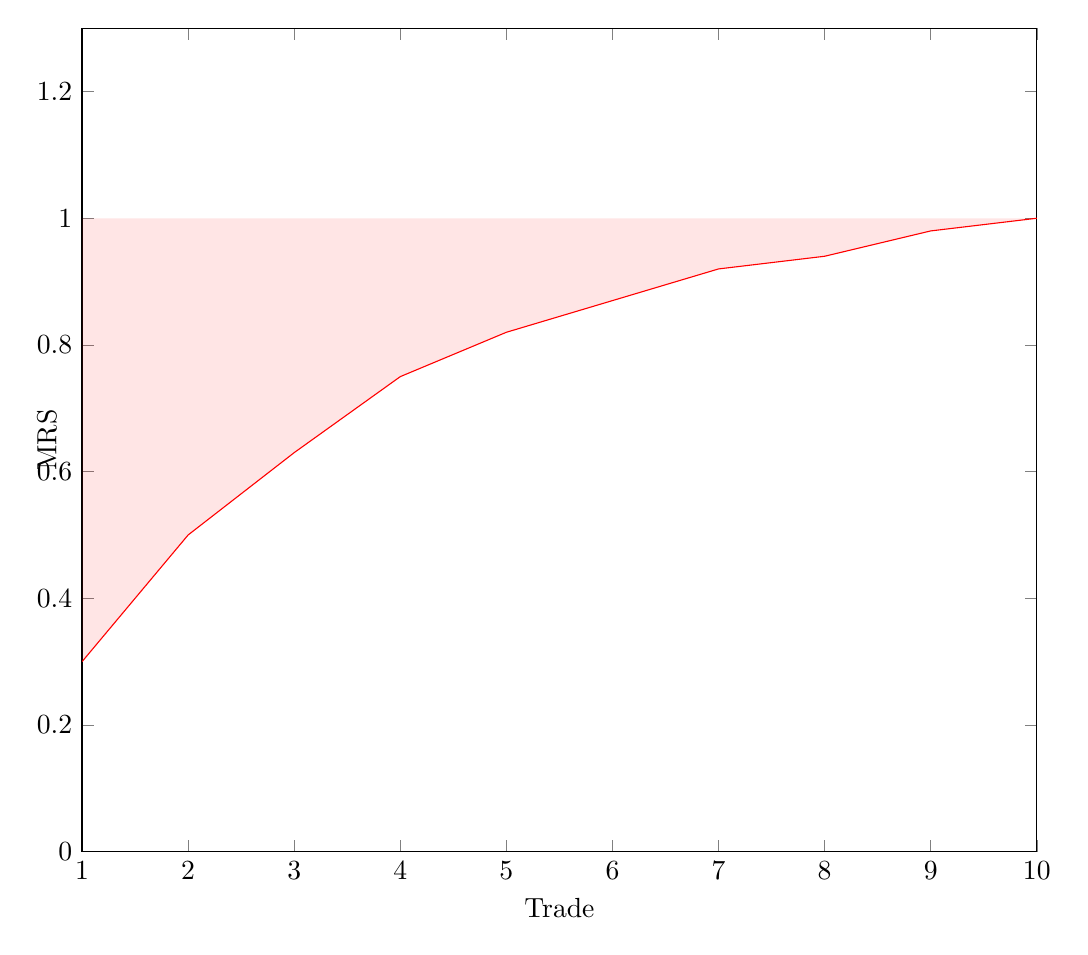
\begin{tikzpicture} 
      \begin{axis}[
        width=\linewidth,
        scale only axis,
        xlabel={Trade},
        ylabel={MRS},
        xmin=1, xmax=10,
        ymin=0, ymax=1.3,
        ylabel style={overlay, anchor=north,},
        ]
        \addplot[
          name path=f,
          color=red,
        ]
        coordinates {
          (1,0.3)(2,0.5)(3,0.63)(4,0.75)(5,0.82)(6,0.87)(7,0.92)(8,0.94)(9,0.98)(10,1.0)
        }; 
      
        \path[name path=axis] (axis cs:1,1.0) -- (axis cs:10,1.0);
      
        \addplot [
          thick,
          color=red,
          fill=red, 
          fill opacity=0.1
          ]
        fill between[
          of=f and axis,
          split,
        ];
      \end{axis}
    \end{tikzpicture}
    \caption{Without constraint}
  \end{subfigure}%
  \hspace{2.0cm}
  \begin{subfigure}{.4\linewidth}\centering
    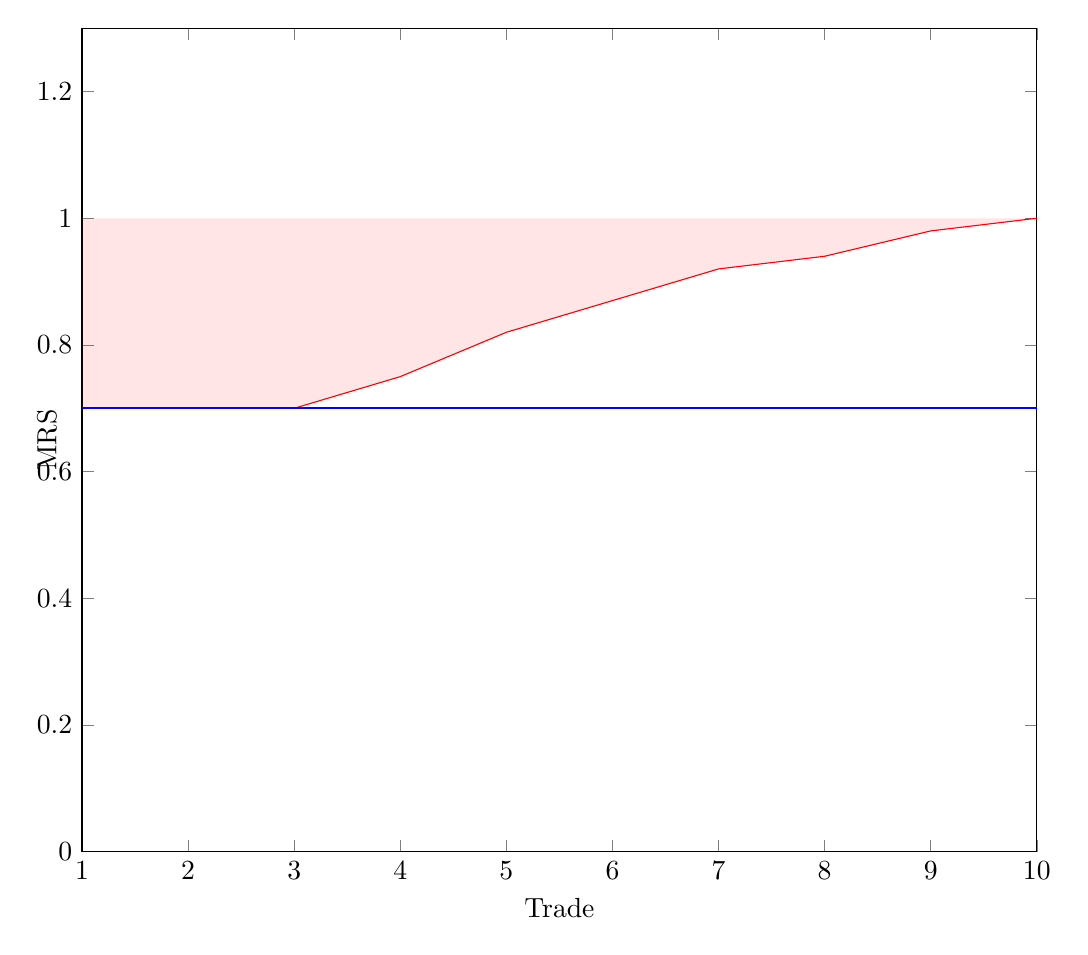
\begin{tikzpicture} 
      \begin{axis}[
        width=\linewidth,
        scale only axis,
        xlabel={Trade},
        ylabel={MRS},
        xmin=1, xmax=10,
        ymin=0, ymax=1.3,
        ylabel style={overlay, anchor=north,},
        ]
        \addplot[
          name path=f,
          color=red,
          ]
        coordinates {
          (1,0.7)(2,0.7)(3,0.7)(4,0.75)(5,0.82)(6,0.87)(7,0.92)(8,0.94)(9,0.98)(10,1.0)
        }; 
        
        \path[name path=axis] (axis cs:1,1.0) -- (axis cs:10,1.0);

        \draw[name path=constraint, color=blue, thick] (axis cs:1,0.7) -- (axis cs:10,0.7);
      
        \addplot [
          thick,
          color=red,
          fill=red, 
          fill opacity=0.1
          ]
        fill between[
          of=f and axis,
          split,
        ];
      \end{axis}
    \end{tikzpicture}  
    \caption{With selling constraint at 0.7}
  \end{subfigure}%
  
  \caption{
    This shows the MRSs that a subsidiser trades at over two days.
    The trader is selling, so they prefer a higher MRS.
    The shaded area is the wealth lost by not trading at the final price immediately.
    On the second day, the trader adds a selling constraint at 0.7, which causes them to lose less wealth.
  }
  \label{fig:wealth}
\end{figure}

\subsection{Updating Constraints}
In order to get better outcomes from one day to the next, the traders must change their behaviour.
They achieve this by updating the constraints on the MRSs they will accept.

Each trader has two constraints: buying and selling.
The buying constraint is the highest MRS they will pay to buy Good 1.
The selling constraint is the lowest MRS they will accept to sell Good 1.

Using the definition of wealth from above, and the last MRS used globally, each trader calculates the wealth they gained or lost during the day.

Recall that no traders will accept trades that cause them to lose utility. 
Thus, they will have a non-negative utility gain, which we can calculate by subtracting the utility of the initial endowment from the utility of the final allocation after a day's worth of trades.

First, if the trader updated their constraint on the previous day, they evaluate its effectiveness.
They compare their wealth and utility gains from today to those from yesterday.
If the new constraint resulted in less utility or the same utility and less wealth, the constraint is reverted to its previous value.

If they did not update their constraint on the previous day, the trader considers tightening it.
\begin{itemize}
  \item If the trader gained wealth during the day, they are happy with the MRSs they are accepting, so they don't make any changes.
  \item If the trader lost wealth, they determine whether they were a net buyer or seller of Good 1:
    \begin{itemize}
      \item If the trader was a net buyer, they decrease their buying constraint.
      \item If the trader was a net seller, they increase their selling constraint instead.
    \end{itemize}
\end{itemize}

See Figure \ref{fig:wealth} for an example of this procedure.
We will discuss the exact method of tightening in Section \ref{results}, when we compare different techniques.

\subsection{Statistics}
At the end of each day, we calculate five statistics about the day's trading: utility gain, wealth transfer, MRS deviation, constrainedness, and attempted trades.
These are used to evaluate the performance of the model.

The global utility gain, is the percentage increase in utility over the day for all the traders. 
Because it is a percentage, it can be compared across different starting allocations and numbers of traders.
It increases initially then settles as the traders learn constraints that help them maximize their utility gains.
It can decrease if the traders become over-constrained.

The wealth transfer is the sum of the absolute value of wealth gained or lost, divided by the total wealth at the beginning.
Like above, it is marked to the MRS of the final successful trade.
This should approach 0 as subsiders apply constraints to prevent themselves from losing wealth.

As mentioned above, each trader has a most recent MRS they personally traded at.
In the ideal case, these all converge to the same value over the day, because if two traders disagree about MRS they can make a mutually beneficial trade.
To evaluate how close a simulation comes to this ideal, we calculate the standard deviation of the most recent MRS for each trader.

We calculate constrainedness based on the constraints used by each trader in the past day.
There are initial buy and sell constraints that every trader begins with.
This is the percentage of the original range between constraints that traders accept on average.
We actually use the log range, because the initial constraints vary by orders of magnitude and the plain range would underweight the lower (sell) constraint.
For example, constrainedness of 100\% means that 100\% of MRSs (within those initial constraints) are accepted.
Constrainedness of 5\% means that only 5\% of MRSs are acceptable on average.
We expect this to decrease over multiple days, and converge to a low value.

Lastly, we record the average number of attempted trades per trader in the day.
We use this as our main method of comparing the running time of different models.
The elapsed clock time is also recorded, but this is less useful because it isn't comparable across machines.

We track these statistics over many days of trading, and use them to analyse the results.
They are displayed in charts like that in Figure \ref{fig:conv}.

\begin{figure}[H]
    \centering
    %% Creator: Matplotlib, PGF backend
%%
%% To include the figure in your LaTeX document, write
%%   \input{<filename>.pgf}
%%
%% Make sure the required packages are loaded in your preamble
%%   \usepackage{pgf}
%%
%% Figures using additional raster images can only be included by \input if
%% they are in the same directory as the main LaTeX file. For loading figures
%% from other directories you can use the `import` package
%%   \usepackage{import}
%% and then include the figures with
%%   \import{<path to file>}{<filename>.pgf}
%%
%% Matplotlib used the following preamble
%%   \usepackage[utf8x]{inputenc}
%%   \usepackage[T1]{fontenc}
%%
\begingroup%
\makeatletter%
\begin{pgfpicture}%
\pgfpathrectangle{\pgfpointorigin}{\pgfqpoint{5.555872in}{4.386181in}}%
\pgfusepath{use as bounding box, clip}%
\begin{pgfscope}%
\pgfsetbuttcap%
\pgfsetmiterjoin%
\definecolor{currentfill}{rgb}{1.000000,1.000000,1.000000}%
\pgfsetfillcolor{currentfill}%
\pgfsetlinewidth{0.000000pt}%
\definecolor{currentstroke}{rgb}{1.000000,1.000000,1.000000}%
\pgfsetstrokecolor{currentstroke}%
\pgfsetdash{}{0pt}%
\pgfpathmoveto{\pgfqpoint{0.000000in}{0.000000in}}%
\pgfpathlineto{\pgfqpoint{5.555872in}{0.000000in}}%
\pgfpathlineto{\pgfqpoint{5.555872in}{4.386181in}}%
\pgfpathlineto{\pgfqpoint{0.000000in}{4.386181in}}%
\pgfpathclose%
\pgfusepath{fill}%
\end{pgfscope}%
\begin{pgfscope}%
\pgfsetbuttcap%
\pgfsetmiterjoin%
\definecolor{currentfill}{rgb}{1.000000,1.000000,1.000000}%
\pgfsetfillcolor{currentfill}%
\pgfsetlinewidth{0.000000pt}%
\definecolor{currentstroke}{rgb}{0.000000,0.000000,0.000000}%
\pgfsetstrokecolor{currentstroke}%
\pgfsetstrokeopacity{0.000000}%
\pgfsetdash{}{0pt}%
\pgfpathmoveto{\pgfqpoint{0.333025in}{0.494841in}}%
\pgfpathlineto{\pgfqpoint{5.351705in}{0.494841in}}%
\pgfpathlineto{\pgfqpoint{5.351705in}{4.224854in}}%
\pgfpathlineto{\pgfqpoint{0.333025in}{4.224854in}}%
\pgfpathclose%
\pgfusepath{fill}%
\end{pgfscope}%
\begin{pgfscope}%
\pgfpathrectangle{\pgfqpoint{0.333025in}{0.494841in}}{\pgfqpoint{5.018680in}{3.730012in}} %
\pgfusepath{clip}%
\pgfsetrectcap%
\pgfsetroundjoin%
\pgfsetlinewidth{1.003750pt}%
\definecolor{currentstroke}{rgb}{0.000000,0.000000,1.000000}%
\pgfsetstrokecolor{currentstroke}%
\pgfsetdash{}{0pt}%
\pgfpathmoveto{\pgfqpoint{0.333025in}{0.905553in}}%
\pgfpathlineto{\pgfqpoint{0.343063in}{0.812220in}}%
\pgfpathlineto{\pgfqpoint{0.353100in}{0.807098in}}%
\pgfpathlineto{\pgfqpoint{0.363137in}{0.777261in}}%
\pgfpathlineto{\pgfqpoint{0.373175in}{0.808544in}}%
\pgfpathlineto{\pgfqpoint{0.383212in}{0.760810in}}%
\pgfpathlineto{\pgfqpoint{0.393249in}{0.804897in}}%
\pgfpathlineto{\pgfqpoint{0.403287in}{0.792812in}}%
\pgfpathlineto{\pgfqpoint{0.413324in}{0.788944in}}%
\pgfpathlineto{\pgfqpoint{0.423362in}{0.780363in}}%
\pgfpathlineto{\pgfqpoint{0.433399in}{0.760920in}}%
\pgfpathlineto{\pgfqpoint{0.443436in}{0.771832in}}%
\pgfpathlineto{\pgfqpoint{0.463511in}{0.748948in}}%
\pgfpathlineto{\pgfqpoint{0.473548in}{0.762202in}}%
\pgfpathlineto{\pgfqpoint{0.483586in}{0.769212in}}%
\pgfpathlineto{\pgfqpoint{0.493623in}{0.750854in}}%
\pgfpathlineto{\pgfqpoint{0.503660in}{0.750490in}}%
\pgfpathlineto{\pgfqpoint{0.513698in}{0.762608in}}%
\pgfpathlineto{\pgfqpoint{0.523735in}{0.756932in}}%
\pgfpathlineto{\pgfqpoint{0.533772in}{0.755402in}}%
\pgfpathlineto{\pgfqpoint{0.543810in}{0.755995in}}%
\pgfpathlineto{\pgfqpoint{0.563885in}{0.747363in}}%
\pgfpathlineto{\pgfqpoint{0.573922in}{0.750526in}}%
\pgfpathlineto{\pgfqpoint{0.583959in}{0.767920in}}%
\pgfpathlineto{\pgfqpoint{0.593997in}{0.768669in}}%
\pgfpathlineto{\pgfqpoint{0.604034in}{0.751662in}}%
\pgfpathlineto{\pgfqpoint{0.624109in}{0.771388in}}%
\pgfpathlineto{\pgfqpoint{0.634146in}{0.755534in}}%
\pgfpathlineto{\pgfqpoint{0.644183in}{0.749668in}}%
\pgfpathlineto{\pgfqpoint{0.654221in}{0.756298in}}%
\pgfpathlineto{\pgfqpoint{0.664258in}{0.752698in}}%
\pgfpathlineto{\pgfqpoint{0.674296in}{0.767297in}}%
\pgfpathlineto{\pgfqpoint{0.684333in}{0.755126in}}%
\pgfpathlineto{\pgfqpoint{0.694370in}{0.758082in}}%
\pgfpathlineto{\pgfqpoint{0.704408in}{0.748271in}}%
\pgfpathlineto{\pgfqpoint{0.714445in}{0.756869in}}%
\pgfpathlineto{\pgfqpoint{0.724482in}{0.754573in}}%
\pgfpathlineto{\pgfqpoint{0.734520in}{0.742342in}}%
\pgfpathlineto{\pgfqpoint{0.744557in}{0.745273in}}%
\pgfpathlineto{\pgfqpoint{0.754594in}{0.750934in}}%
\pgfpathlineto{\pgfqpoint{0.764632in}{0.752932in}}%
\pgfpathlineto{\pgfqpoint{0.784706in}{0.735682in}}%
\pgfpathlineto{\pgfqpoint{0.794744in}{0.753449in}}%
\pgfpathlineto{\pgfqpoint{0.804781in}{0.743315in}}%
\pgfpathlineto{\pgfqpoint{0.814819in}{0.751992in}}%
\pgfpathlineto{\pgfqpoint{0.824856in}{0.742024in}}%
\pgfpathlineto{\pgfqpoint{0.834893in}{0.738411in}}%
\pgfpathlineto{\pgfqpoint{0.844931in}{0.738056in}}%
\pgfpathlineto{\pgfqpoint{0.875043in}{0.746327in}}%
\pgfpathlineto{\pgfqpoint{0.885080in}{0.732026in}}%
\pgfpathlineto{\pgfqpoint{0.895117in}{0.732808in}}%
\pgfpathlineto{\pgfqpoint{0.905155in}{0.730375in}}%
\pgfpathlineto{\pgfqpoint{0.915192in}{0.739571in}}%
\pgfpathlineto{\pgfqpoint{0.925230in}{0.736510in}}%
\pgfpathlineto{\pgfqpoint{0.935267in}{0.729058in}}%
\pgfpathlineto{\pgfqpoint{0.945304in}{0.733093in}}%
\pgfpathlineto{\pgfqpoint{0.955342in}{0.729096in}}%
\pgfpathlineto{\pgfqpoint{0.965379in}{0.742392in}}%
\pgfpathlineto{\pgfqpoint{0.975416in}{0.732712in}}%
\pgfpathlineto{\pgfqpoint{0.985454in}{0.734997in}}%
\pgfpathlineto{\pgfqpoint{0.995491in}{0.733448in}}%
\pgfpathlineto{\pgfqpoint{1.005528in}{0.733688in}}%
\pgfpathlineto{\pgfqpoint{1.015566in}{0.722482in}}%
\pgfpathlineto{\pgfqpoint{1.025603in}{0.729256in}}%
\pgfpathlineto{\pgfqpoint{1.035640in}{0.738020in}}%
\pgfpathlineto{\pgfqpoint{1.045678in}{0.736525in}}%
\pgfpathlineto{\pgfqpoint{1.055715in}{0.738051in}}%
\pgfpathlineto{\pgfqpoint{1.065753in}{0.726554in}}%
\pgfpathlineto{\pgfqpoint{1.075790in}{0.738398in}}%
\pgfpathlineto{\pgfqpoint{1.085827in}{0.735942in}}%
\pgfpathlineto{\pgfqpoint{1.095865in}{0.724669in}}%
\pgfpathlineto{\pgfqpoint{1.105902in}{0.736604in}}%
\pgfpathlineto{\pgfqpoint{1.115939in}{0.741980in}}%
\pgfpathlineto{\pgfqpoint{1.125977in}{0.723376in}}%
\pgfpathlineto{\pgfqpoint{1.136014in}{0.734997in}}%
\pgfpathlineto{\pgfqpoint{1.146051in}{0.718416in}}%
\pgfpathlineto{\pgfqpoint{1.156089in}{0.737853in}}%
\pgfpathlineto{\pgfqpoint{1.166126in}{0.725807in}}%
\pgfpathlineto{\pgfqpoint{1.176164in}{0.730974in}}%
\pgfpathlineto{\pgfqpoint{1.186201in}{0.730932in}}%
\pgfpathlineto{\pgfqpoint{1.206276in}{0.732997in}}%
\pgfpathlineto{\pgfqpoint{1.216313in}{0.742182in}}%
\pgfpathlineto{\pgfqpoint{1.226350in}{0.735083in}}%
\pgfpathlineto{\pgfqpoint{1.236388in}{0.731473in}}%
\pgfpathlineto{\pgfqpoint{1.246425in}{0.726446in}}%
\pgfpathlineto{\pgfqpoint{1.256462in}{0.732813in}}%
\pgfpathlineto{\pgfqpoint{1.266500in}{0.722823in}}%
\pgfpathlineto{\pgfqpoint{1.276537in}{0.722309in}}%
\pgfpathlineto{\pgfqpoint{1.286574in}{0.714168in}}%
\pgfpathlineto{\pgfqpoint{1.296612in}{0.723347in}}%
\pgfpathlineto{\pgfqpoint{1.306649in}{0.725251in}}%
\pgfpathlineto{\pgfqpoint{1.316687in}{0.725899in}}%
\pgfpathlineto{\pgfqpoint{1.326724in}{0.729740in}}%
\pgfpathlineto{\pgfqpoint{1.336761in}{0.728132in}}%
\pgfpathlineto{\pgfqpoint{1.346799in}{0.744949in}}%
\pgfpathlineto{\pgfqpoint{1.356836in}{0.756936in}}%
\pgfpathlineto{\pgfqpoint{1.366873in}{0.719065in}}%
\pgfpathlineto{\pgfqpoint{1.376911in}{0.723714in}}%
\pgfpathlineto{\pgfqpoint{1.386948in}{0.731043in}}%
\pgfpathlineto{\pgfqpoint{1.396985in}{0.733624in}}%
\pgfpathlineto{\pgfqpoint{1.407023in}{0.752188in}}%
\pgfpathlineto{\pgfqpoint{1.417060in}{0.732736in}}%
\pgfpathlineto{\pgfqpoint{1.427098in}{0.737462in}}%
\pgfpathlineto{\pgfqpoint{1.437135in}{0.727662in}}%
\pgfpathlineto{\pgfqpoint{1.457210in}{0.741949in}}%
\pgfpathlineto{\pgfqpoint{1.467247in}{0.729345in}}%
\pgfpathlineto{\pgfqpoint{1.477284in}{0.740941in}}%
\pgfpathlineto{\pgfqpoint{1.487322in}{0.721103in}}%
\pgfpathlineto{\pgfqpoint{1.497359in}{0.738172in}}%
\pgfpathlineto{\pgfqpoint{1.507396in}{0.737400in}}%
\pgfpathlineto{\pgfqpoint{1.517434in}{0.742042in}}%
\pgfpathlineto{\pgfqpoint{1.527471in}{0.743716in}}%
\pgfpathlineto{\pgfqpoint{1.537508in}{0.740746in}}%
\pgfpathlineto{\pgfqpoint{1.547546in}{0.742371in}}%
\pgfpathlineto{\pgfqpoint{1.557583in}{0.731984in}}%
\pgfpathlineto{\pgfqpoint{1.567621in}{0.726272in}}%
\pgfpathlineto{\pgfqpoint{1.587695in}{0.729846in}}%
\pgfpathlineto{\pgfqpoint{1.597733in}{0.726642in}}%
\pgfpathlineto{\pgfqpoint{1.607770in}{0.729507in}}%
\pgfpathlineto{\pgfqpoint{1.617807in}{0.734407in}}%
\pgfpathlineto{\pgfqpoint{1.627845in}{0.727048in}}%
\pgfpathlineto{\pgfqpoint{1.637882in}{0.730411in}}%
\pgfpathlineto{\pgfqpoint{1.647919in}{0.738223in}}%
\pgfpathlineto{\pgfqpoint{1.657957in}{0.720141in}}%
\pgfpathlineto{\pgfqpoint{1.667994in}{0.725723in}}%
\pgfpathlineto{\pgfqpoint{1.678032in}{0.721658in}}%
\pgfpathlineto{\pgfqpoint{1.698106in}{0.726214in}}%
\pgfpathlineto{\pgfqpoint{1.708144in}{0.733294in}}%
\pgfpathlineto{\pgfqpoint{1.718181in}{0.724685in}}%
\pgfpathlineto{\pgfqpoint{1.728218in}{0.726627in}}%
\pgfpathlineto{\pgfqpoint{1.738256in}{0.723129in}}%
\pgfpathlineto{\pgfqpoint{1.748293in}{0.730467in}}%
\pgfpathlineto{\pgfqpoint{1.758330in}{0.733249in}}%
\pgfpathlineto{\pgfqpoint{1.768368in}{0.715449in}}%
\pgfpathlineto{\pgfqpoint{1.778405in}{0.724310in}}%
\pgfpathlineto{\pgfqpoint{1.788442in}{0.726963in}}%
\pgfpathlineto{\pgfqpoint{1.798480in}{0.726384in}}%
\pgfpathlineto{\pgfqpoint{1.808517in}{0.730199in}}%
\pgfpathlineto{\pgfqpoint{1.818555in}{0.727586in}}%
\pgfpathlineto{\pgfqpoint{1.828592in}{0.721596in}}%
\pgfpathlineto{\pgfqpoint{1.838629in}{0.721494in}}%
\pgfpathlineto{\pgfqpoint{1.848667in}{0.728974in}}%
\pgfpathlineto{\pgfqpoint{1.858704in}{0.715573in}}%
\pgfpathlineto{\pgfqpoint{1.868741in}{0.727842in}}%
\pgfpathlineto{\pgfqpoint{1.878779in}{0.728305in}}%
\pgfpathlineto{\pgfqpoint{1.898853in}{0.726830in}}%
\pgfpathlineto{\pgfqpoint{1.908891in}{0.727057in}}%
\pgfpathlineto{\pgfqpoint{1.918928in}{0.725282in}}%
\pgfpathlineto{\pgfqpoint{1.928966in}{0.729802in}}%
\pgfpathlineto{\pgfqpoint{1.939003in}{0.717535in}}%
\pgfpathlineto{\pgfqpoint{1.949040in}{0.730518in}}%
\pgfpathlineto{\pgfqpoint{1.969115in}{0.716457in}}%
\pgfpathlineto{\pgfqpoint{1.979152in}{0.722414in}}%
\pgfpathlineto{\pgfqpoint{1.989190in}{0.710617in}}%
\pgfpathlineto{\pgfqpoint{1.999227in}{0.730181in}}%
\pgfpathlineto{\pgfqpoint{2.009264in}{0.721976in}}%
\pgfpathlineto{\pgfqpoint{2.019302in}{0.728204in}}%
\pgfpathlineto{\pgfqpoint{2.029339in}{0.726756in}}%
\pgfpathlineto{\pgfqpoint{2.039376in}{0.720603in}}%
\pgfpathlineto{\pgfqpoint{2.049414in}{0.726889in}}%
\pgfpathlineto{\pgfqpoint{2.059451in}{0.717890in}}%
\pgfpathlineto{\pgfqpoint{2.069489in}{0.723402in}}%
\pgfpathlineto{\pgfqpoint{2.079526in}{0.724135in}}%
\pgfpathlineto{\pgfqpoint{2.089563in}{0.726567in}}%
\pgfpathlineto{\pgfqpoint{2.099601in}{0.717361in}}%
\pgfpathlineto{\pgfqpoint{2.109638in}{0.723469in}}%
\pgfpathlineto{\pgfqpoint{2.119675in}{0.724165in}}%
\pgfpathlineto{\pgfqpoint{2.129713in}{0.729043in}}%
\pgfpathlineto{\pgfqpoint{2.139750in}{0.736808in}}%
\pgfpathlineto{\pgfqpoint{2.149787in}{0.727541in}}%
\pgfpathlineto{\pgfqpoint{2.159825in}{0.729511in}}%
\pgfpathlineto{\pgfqpoint{2.169862in}{0.720115in}}%
\pgfpathlineto{\pgfqpoint{2.179899in}{0.721486in}}%
\pgfpathlineto{\pgfqpoint{2.189937in}{0.718930in}}%
\pgfpathlineto{\pgfqpoint{2.199974in}{0.714967in}}%
\pgfpathlineto{\pgfqpoint{2.210012in}{0.726658in}}%
\pgfpathlineto{\pgfqpoint{2.220049in}{0.721160in}}%
\pgfpathlineto{\pgfqpoint{2.230086in}{0.729933in}}%
\pgfpathlineto{\pgfqpoint{2.240124in}{0.707151in}}%
\pgfpathlineto{\pgfqpoint{2.250161in}{0.716361in}}%
\pgfpathlineto{\pgfqpoint{2.260198in}{0.723870in}}%
\pgfpathlineto{\pgfqpoint{2.270236in}{0.724942in}}%
\pgfpathlineto{\pgfqpoint{2.280273in}{0.714740in}}%
\pgfpathlineto{\pgfqpoint{2.290310in}{0.730179in}}%
\pgfpathlineto{\pgfqpoint{2.300348in}{0.716221in}}%
\pgfpathlineto{\pgfqpoint{2.310385in}{0.731097in}}%
\pgfpathlineto{\pgfqpoint{2.320423in}{0.722667in}}%
\pgfpathlineto{\pgfqpoint{2.330460in}{0.720384in}}%
\pgfpathlineto{\pgfqpoint{2.340497in}{0.724716in}}%
\pgfpathlineto{\pgfqpoint{2.350535in}{0.714884in}}%
\pgfpathlineto{\pgfqpoint{2.360572in}{0.722968in}}%
\pgfpathlineto{\pgfqpoint{2.370609in}{0.719661in}}%
\pgfpathlineto{\pgfqpoint{2.380647in}{0.717718in}}%
\pgfpathlineto{\pgfqpoint{2.390684in}{0.725655in}}%
\pgfpathlineto{\pgfqpoint{2.400721in}{0.727557in}}%
\pgfpathlineto{\pgfqpoint{2.410759in}{0.722905in}}%
\pgfpathlineto{\pgfqpoint{2.420796in}{0.728730in}}%
\pgfpathlineto{\pgfqpoint{2.430833in}{0.716388in}}%
\pgfpathlineto{\pgfqpoint{2.440871in}{0.715195in}}%
\pgfpathlineto{\pgfqpoint{2.450908in}{0.726703in}}%
\pgfpathlineto{\pgfqpoint{2.460946in}{0.717156in}}%
\pgfpathlineto{\pgfqpoint{2.470983in}{0.722610in}}%
\pgfpathlineto{\pgfqpoint{2.481020in}{0.724986in}}%
\pgfpathlineto{\pgfqpoint{2.491058in}{0.708454in}}%
\pgfpathlineto{\pgfqpoint{2.501095in}{0.726498in}}%
\pgfpathlineto{\pgfqpoint{2.511132in}{0.718233in}}%
\pgfpathlineto{\pgfqpoint{2.521170in}{0.724014in}}%
\pgfpathlineto{\pgfqpoint{2.531207in}{0.724467in}}%
\pgfpathlineto{\pgfqpoint{2.541244in}{0.722427in}}%
\pgfpathlineto{\pgfqpoint{2.551282in}{0.718276in}}%
\pgfpathlineto{\pgfqpoint{2.561319in}{0.734189in}}%
\pgfpathlineto{\pgfqpoint{2.571357in}{0.730002in}}%
\pgfpathlineto{\pgfqpoint{2.581394in}{0.717272in}}%
\pgfpathlineto{\pgfqpoint{2.591431in}{0.726278in}}%
\pgfpathlineto{\pgfqpoint{2.601469in}{0.729091in}}%
\pgfpathlineto{\pgfqpoint{2.611506in}{0.724015in}}%
\pgfpathlineto{\pgfqpoint{2.621543in}{0.723760in}}%
\pgfpathlineto{\pgfqpoint{2.631581in}{0.725611in}}%
\pgfpathlineto{\pgfqpoint{2.641618in}{0.723693in}}%
\pgfpathlineto{\pgfqpoint{2.651655in}{0.719623in}}%
\pgfpathlineto{\pgfqpoint{2.661693in}{0.718990in}}%
\pgfpathlineto{\pgfqpoint{2.691805in}{0.722707in}}%
\pgfpathlineto{\pgfqpoint{2.701842in}{0.722010in}}%
\pgfpathlineto{\pgfqpoint{2.711880in}{0.715335in}}%
\pgfpathlineto{\pgfqpoint{2.721917in}{0.727175in}}%
\pgfpathlineto{\pgfqpoint{2.731954in}{0.725750in}}%
\pgfpathlineto{\pgfqpoint{2.741992in}{0.726195in}}%
\pgfpathlineto{\pgfqpoint{2.752029in}{0.720139in}}%
\pgfpathlineto{\pgfqpoint{2.762066in}{0.720717in}}%
\pgfpathlineto{\pgfqpoint{2.772104in}{0.733411in}}%
\pgfpathlineto{\pgfqpoint{2.782141in}{0.712881in}}%
\pgfpathlineto{\pgfqpoint{2.792178in}{0.719632in}}%
\pgfpathlineto{\pgfqpoint{2.812253in}{0.725321in}}%
\pgfpathlineto{\pgfqpoint{2.822291in}{0.727002in}}%
\pgfpathlineto{\pgfqpoint{2.832328in}{0.719761in}}%
\pgfpathlineto{\pgfqpoint{2.842365in}{0.722080in}}%
\pgfpathlineto{\pgfqpoint{2.852403in}{0.721625in}}%
\pgfpathlineto{\pgfqpoint{2.862440in}{0.717059in}}%
\pgfpathlineto{\pgfqpoint{2.872477in}{0.724245in}}%
\pgfpathlineto{\pgfqpoint{2.882515in}{0.728796in}}%
\pgfpathlineto{\pgfqpoint{2.892552in}{0.728117in}}%
\pgfpathlineto{\pgfqpoint{2.902589in}{0.722471in}}%
\pgfpathlineto{\pgfqpoint{2.912627in}{0.721004in}}%
\pgfpathlineto{\pgfqpoint{2.922664in}{0.716974in}}%
\pgfpathlineto{\pgfqpoint{2.932701in}{0.722054in}}%
\pgfpathlineto{\pgfqpoint{2.942739in}{0.722910in}}%
\pgfpathlineto{\pgfqpoint{2.962814in}{0.728713in}}%
\pgfpathlineto{\pgfqpoint{2.972851in}{0.725855in}}%
\pgfpathlineto{\pgfqpoint{2.982888in}{0.730467in}}%
\pgfpathlineto{\pgfqpoint{2.992926in}{0.731772in}}%
\pgfpathlineto{\pgfqpoint{3.002963in}{0.725851in}}%
\pgfpathlineto{\pgfqpoint{3.013000in}{0.725831in}}%
\pgfpathlineto{\pgfqpoint{3.023038in}{0.724493in}}%
\pgfpathlineto{\pgfqpoint{3.043112in}{0.718574in}}%
\pgfpathlineto{\pgfqpoint{3.053150in}{0.724964in}}%
\pgfpathlineto{\pgfqpoint{3.063187in}{0.717056in}}%
\pgfpathlineto{\pgfqpoint{3.073225in}{0.718669in}}%
\pgfpathlineto{\pgfqpoint{3.083262in}{0.716343in}}%
\pgfpathlineto{\pgfqpoint{3.093299in}{0.709832in}}%
\pgfpathlineto{\pgfqpoint{3.103337in}{0.720447in}}%
\pgfpathlineto{\pgfqpoint{3.113374in}{0.716685in}}%
\pgfpathlineto{\pgfqpoint{3.123411in}{0.717830in}}%
\pgfpathlineto{\pgfqpoint{3.143486in}{0.727796in}}%
\pgfpathlineto{\pgfqpoint{3.153523in}{0.719192in}}%
\pgfpathlineto{\pgfqpoint{3.163561in}{0.726631in}}%
\pgfpathlineto{\pgfqpoint{3.173598in}{0.717272in}}%
\pgfpathlineto{\pgfqpoint{3.183635in}{0.725254in}}%
\pgfpathlineto{\pgfqpoint{3.193673in}{0.718718in}}%
\pgfpathlineto{\pgfqpoint{3.203710in}{0.732740in}}%
\pgfpathlineto{\pgfqpoint{3.213748in}{0.716046in}}%
\pgfpathlineto{\pgfqpoint{3.223785in}{0.714955in}}%
\pgfpathlineto{\pgfqpoint{3.233822in}{0.729957in}}%
\pgfpathlineto{\pgfqpoint{3.243860in}{0.727737in}}%
\pgfpathlineto{\pgfqpoint{3.253897in}{0.720391in}}%
\pgfpathlineto{\pgfqpoint{3.263934in}{0.727908in}}%
\pgfpathlineto{\pgfqpoint{3.273972in}{0.723123in}}%
\pgfpathlineto{\pgfqpoint{3.284009in}{0.719658in}}%
\pgfpathlineto{\pgfqpoint{3.294046in}{0.725394in}}%
\pgfpathlineto{\pgfqpoint{3.304084in}{0.715969in}}%
\pgfpathlineto{\pgfqpoint{3.314121in}{0.721488in}}%
\pgfpathlineto{\pgfqpoint{3.324159in}{0.719915in}}%
\pgfpathlineto{\pgfqpoint{3.334196in}{0.722446in}}%
\pgfpathlineto{\pgfqpoint{3.344233in}{0.729621in}}%
\pgfpathlineto{\pgfqpoint{3.354271in}{0.715868in}}%
\pgfpathlineto{\pgfqpoint{3.364308in}{0.733550in}}%
\pgfpathlineto{\pgfqpoint{3.374345in}{0.722075in}}%
\pgfpathlineto{\pgfqpoint{3.384383in}{0.728193in}}%
\pgfpathlineto{\pgfqpoint{3.394420in}{0.725017in}}%
\pgfpathlineto{\pgfqpoint{3.404457in}{0.717021in}}%
\pgfpathlineto{\pgfqpoint{3.414495in}{0.720516in}}%
\pgfpathlineto{\pgfqpoint{3.424532in}{0.721548in}}%
\pgfpathlineto{\pgfqpoint{3.434569in}{0.719344in}}%
\pgfpathlineto{\pgfqpoint{3.444607in}{0.725306in}}%
\pgfpathlineto{\pgfqpoint{3.454644in}{0.727185in}}%
\pgfpathlineto{\pgfqpoint{3.464682in}{0.717933in}}%
\pgfpathlineto{\pgfqpoint{3.474719in}{0.715753in}}%
\pgfpathlineto{\pgfqpoint{3.484756in}{0.723605in}}%
\pgfpathlineto{\pgfqpoint{3.494794in}{0.727758in}}%
\pgfpathlineto{\pgfqpoint{3.504831in}{0.715767in}}%
\pgfpathlineto{\pgfqpoint{3.514868in}{0.714425in}}%
\pgfpathlineto{\pgfqpoint{3.524906in}{0.729167in}}%
\pgfpathlineto{\pgfqpoint{3.534943in}{0.718474in}}%
\pgfpathlineto{\pgfqpoint{3.544980in}{0.721683in}}%
\pgfpathlineto{\pgfqpoint{3.575093in}{0.722060in}}%
\pgfpathlineto{\pgfqpoint{3.585130in}{0.718140in}}%
\pgfpathlineto{\pgfqpoint{3.595167in}{0.712101in}}%
\pgfpathlineto{\pgfqpoint{3.605205in}{0.723625in}}%
\pgfpathlineto{\pgfqpoint{3.615242in}{0.716344in}}%
\pgfpathlineto{\pgfqpoint{3.625279in}{0.715942in}}%
\pgfpathlineto{\pgfqpoint{3.635317in}{0.725448in}}%
\pgfpathlineto{\pgfqpoint{3.645354in}{0.723978in}}%
\pgfpathlineto{\pgfqpoint{3.665429in}{0.714650in}}%
\pgfpathlineto{\pgfqpoint{3.675466in}{0.716760in}}%
\pgfpathlineto{\pgfqpoint{3.685503in}{0.727021in}}%
\pgfpathlineto{\pgfqpoint{3.695541in}{0.726451in}}%
\pgfpathlineto{\pgfqpoint{3.705578in}{0.716009in}}%
\pgfpathlineto{\pgfqpoint{3.715616in}{0.722646in}}%
\pgfpathlineto{\pgfqpoint{3.725653in}{0.726205in}}%
\pgfpathlineto{\pgfqpoint{3.735690in}{0.721924in}}%
\pgfpathlineto{\pgfqpoint{3.745728in}{0.720639in}}%
\pgfpathlineto{\pgfqpoint{3.755765in}{0.710388in}}%
\pgfpathlineto{\pgfqpoint{3.765802in}{0.730041in}}%
\pgfpathlineto{\pgfqpoint{3.775840in}{0.720383in}}%
\pgfpathlineto{\pgfqpoint{3.785877in}{0.713665in}}%
\pgfpathlineto{\pgfqpoint{3.795914in}{0.714537in}}%
\pgfpathlineto{\pgfqpoint{3.805952in}{0.718721in}}%
\pgfpathlineto{\pgfqpoint{3.815989in}{0.720483in}}%
\pgfpathlineto{\pgfqpoint{3.826027in}{0.711663in}}%
\pgfpathlineto{\pgfqpoint{3.836064in}{0.721514in}}%
\pgfpathlineto{\pgfqpoint{3.846101in}{0.722679in}}%
\pgfpathlineto{\pgfqpoint{3.856139in}{0.717897in}}%
\pgfpathlineto{\pgfqpoint{3.866176in}{0.725182in}}%
\pgfpathlineto{\pgfqpoint{3.886251in}{0.721661in}}%
\pgfpathlineto{\pgfqpoint{3.896288in}{0.712243in}}%
\pgfpathlineto{\pgfqpoint{3.906325in}{0.724012in}}%
\pgfpathlineto{\pgfqpoint{3.916363in}{0.709889in}}%
\pgfpathlineto{\pgfqpoint{3.936437in}{0.722182in}}%
\pgfpathlineto{\pgfqpoint{3.946475in}{0.722634in}}%
\pgfpathlineto{\pgfqpoint{3.956512in}{0.721563in}}%
\pgfpathlineto{\pgfqpoint{3.966550in}{0.707938in}}%
\pgfpathlineto{\pgfqpoint{3.976587in}{0.714604in}}%
\pgfpathlineto{\pgfqpoint{3.986624in}{0.723622in}}%
\pgfpathlineto{\pgfqpoint{3.996662in}{0.719052in}}%
\pgfpathlineto{\pgfqpoint{4.006699in}{0.717267in}}%
\pgfpathlineto{\pgfqpoint{4.016736in}{0.730390in}}%
\pgfpathlineto{\pgfqpoint{4.026774in}{0.724771in}}%
\pgfpathlineto{\pgfqpoint{4.036811in}{0.722943in}}%
\pgfpathlineto{\pgfqpoint{4.046848in}{0.708495in}}%
\pgfpathlineto{\pgfqpoint{4.056886in}{0.713042in}}%
\pgfpathlineto{\pgfqpoint{4.066923in}{0.709507in}}%
\pgfpathlineto{\pgfqpoint{4.076961in}{0.714955in}}%
\pgfpathlineto{\pgfqpoint{4.086998in}{0.712641in}}%
\pgfpathlineto{\pgfqpoint{4.107073in}{0.721107in}}%
\pgfpathlineto{\pgfqpoint{4.117110in}{0.714652in}}%
\pgfpathlineto{\pgfqpoint{4.127147in}{0.722355in}}%
\pgfpathlineto{\pgfqpoint{4.137185in}{0.722930in}}%
\pgfpathlineto{\pgfqpoint{4.147222in}{0.716335in}}%
\pgfpathlineto{\pgfqpoint{4.157259in}{0.723716in}}%
\pgfpathlineto{\pgfqpoint{4.167297in}{0.723854in}}%
\pgfpathlineto{\pgfqpoint{4.187371in}{0.713046in}}%
\pgfpathlineto{\pgfqpoint{4.197409in}{0.719455in}}%
\pgfpathlineto{\pgfqpoint{4.207446in}{0.724375in}}%
\pgfpathlineto{\pgfqpoint{4.217484in}{0.708863in}}%
\pgfpathlineto{\pgfqpoint{4.227521in}{0.717115in}}%
\pgfpathlineto{\pgfqpoint{4.237558in}{0.716423in}}%
\pgfpathlineto{\pgfqpoint{4.247596in}{0.713740in}}%
\pgfpathlineto{\pgfqpoint{4.257633in}{0.722524in}}%
\pgfpathlineto{\pgfqpoint{4.267670in}{0.713542in}}%
\pgfpathlineto{\pgfqpoint{4.277708in}{0.717842in}}%
\pgfpathlineto{\pgfqpoint{4.287745in}{0.728658in}}%
\pgfpathlineto{\pgfqpoint{4.297782in}{0.716314in}}%
\pgfpathlineto{\pgfqpoint{4.307820in}{0.717898in}}%
\pgfpathlineto{\pgfqpoint{4.317857in}{0.706349in}}%
\pgfpathlineto{\pgfqpoint{4.327895in}{0.710787in}}%
\pgfpathlineto{\pgfqpoint{4.337932in}{0.713631in}}%
\pgfpathlineto{\pgfqpoint{4.347969in}{0.732541in}}%
\pgfpathlineto{\pgfqpoint{4.358007in}{0.715405in}}%
\pgfpathlineto{\pgfqpoint{4.368044in}{0.716233in}}%
\pgfpathlineto{\pgfqpoint{4.378081in}{0.725573in}}%
\pgfpathlineto{\pgfqpoint{4.388119in}{0.720118in}}%
\pgfpathlineto{\pgfqpoint{4.398156in}{0.716036in}}%
\pgfpathlineto{\pgfqpoint{4.408193in}{0.709936in}}%
\pgfpathlineto{\pgfqpoint{4.418231in}{0.711716in}}%
\pgfpathlineto{\pgfqpoint{4.438305in}{0.719752in}}%
\pgfpathlineto{\pgfqpoint{4.448343in}{0.725590in}}%
\pgfpathlineto{\pgfqpoint{4.458380in}{0.718294in}}%
\pgfpathlineto{\pgfqpoint{4.468418in}{0.721262in}}%
\pgfpathlineto{\pgfqpoint{4.478455in}{0.708780in}}%
\pgfpathlineto{\pgfqpoint{4.488492in}{0.722064in}}%
\pgfpathlineto{\pgfqpoint{4.498530in}{0.714415in}}%
\pgfpathlineto{\pgfqpoint{4.508567in}{0.708207in}}%
\pgfpathlineto{\pgfqpoint{4.518604in}{0.712957in}}%
\pgfpathlineto{\pgfqpoint{4.528642in}{0.721620in}}%
\pgfpathlineto{\pgfqpoint{4.538679in}{0.710504in}}%
\pgfpathlineto{\pgfqpoint{4.548716in}{0.720878in}}%
\pgfpathlineto{\pgfqpoint{4.558754in}{0.708395in}}%
\pgfpathlineto{\pgfqpoint{4.568791in}{0.722405in}}%
\pgfpathlineto{\pgfqpoint{4.578829in}{0.718079in}}%
\pgfpathlineto{\pgfqpoint{4.588866in}{0.708491in}}%
\pgfpathlineto{\pgfqpoint{4.598903in}{0.707335in}}%
\pgfpathlineto{\pgfqpoint{4.608941in}{0.716767in}}%
\pgfpathlineto{\pgfqpoint{4.618978in}{0.718795in}}%
\pgfpathlineto{\pgfqpoint{4.629015in}{0.715084in}}%
\pgfpathlineto{\pgfqpoint{4.639053in}{0.715896in}}%
\pgfpathlineto{\pgfqpoint{4.649090in}{0.726192in}}%
\pgfpathlineto{\pgfqpoint{4.659127in}{0.700715in}}%
\pgfpathlineto{\pgfqpoint{4.669165in}{0.718394in}}%
\pgfpathlineto{\pgfqpoint{4.679202in}{0.721801in}}%
\pgfpathlineto{\pgfqpoint{4.689239in}{0.722264in}}%
\pgfpathlineto{\pgfqpoint{4.699277in}{0.720437in}}%
\pgfpathlineto{\pgfqpoint{4.709314in}{0.723407in}}%
\pgfpathlineto{\pgfqpoint{4.719352in}{0.717158in}}%
\pgfpathlineto{\pgfqpoint{4.729389in}{0.728772in}}%
\pgfpathlineto{\pgfqpoint{4.739426in}{0.723424in}}%
\pgfpathlineto{\pgfqpoint{4.749464in}{0.714643in}}%
\pgfpathlineto{\pgfqpoint{4.759501in}{0.716238in}}%
\pgfpathlineto{\pgfqpoint{4.769538in}{0.711689in}}%
\pgfpathlineto{\pgfqpoint{4.779576in}{0.715741in}}%
\pgfpathlineto{\pgfqpoint{4.789613in}{0.722850in}}%
\pgfpathlineto{\pgfqpoint{4.799650in}{0.714557in}}%
\pgfpathlineto{\pgfqpoint{4.809688in}{0.707976in}}%
\pgfpathlineto{\pgfqpoint{4.819725in}{0.719743in}}%
\pgfpathlineto{\pgfqpoint{4.829763in}{0.714085in}}%
\pgfpathlineto{\pgfqpoint{4.839800in}{0.722740in}}%
\pgfpathlineto{\pgfqpoint{4.859875in}{0.709377in}}%
\pgfpathlineto{\pgfqpoint{4.869912in}{0.710566in}}%
\pgfpathlineto{\pgfqpoint{4.879949in}{0.715878in}}%
\pgfpathlineto{\pgfqpoint{4.889987in}{0.711161in}}%
\pgfpathlineto{\pgfqpoint{4.900024in}{0.727587in}}%
\pgfpathlineto{\pgfqpoint{4.930136in}{0.715781in}}%
\pgfpathlineto{\pgfqpoint{4.940173in}{0.717307in}}%
\pgfpathlineto{\pgfqpoint{4.950211in}{0.727163in}}%
\pgfpathlineto{\pgfqpoint{4.960248in}{0.726200in}}%
\pgfpathlineto{\pgfqpoint{4.970286in}{0.711496in}}%
\pgfpathlineto{\pgfqpoint{4.980323in}{0.719629in}}%
\pgfpathlineto{\pgfqpoint{4.990360in}{0.719137in}}%
\pgfpathlineto{\pgfqpoint{5.000398in}{0.712149in}}%
\pgfpathlineto{\pgfqpoint{5.010435in}{0.710732in}}%
\pgfpathlineto{\pgfqpoint{5.020472in}{0.736136in}}%
\pgfpathlineto{\pgfqpoint{5.030510in}{0.722928in}}%
\pgfpathlineto{\pgfqpoint{5.040547in}{0.716927in}}%
\pgfpathlineto{\pgfqpoint{5.050584in}{0.715862in}}%
\pgfpathlineto{\pgfqpoint{5.060622in}{0.717787in}}%
\pgfpathlineto{\pgfqpoint{5.070659in}{0.725658in}}%
\pgfpathlineto{\pgfqpoint{5.080697in}{0.713072in}}%
\pgfpathlineto{\pgfqpoint{5.090734in}{0.713687in}}%
\pgfpathlineto{\pgfqpoint{5.100771in}{0.721873in}}%
\pgfpathlineto{\pgfqpoint{5.110809in}{0.715700in}}%
\pgfpathlineto{\pgfqpoint{5.120846in}{0.725065in}}%
\pgfpathlineto{\pgfqpoint{5.130883in}{0.721320in}}%
\pgfpathlineto{\pgfqpoint{5.140921in}{0.713219in}}%
\pgfpathlineto{\pgfqpoint{5.150958in}{0.727185in}}%
\pgfpathlineto{\pgfqpoint{5.171033in}{0.714094in}}%
\pgfpathlineto{\pgfqpoint{5.181070in}{0.721738in}}%
\pgfpathlineto{\pgfqpoint{5.191107in}{0.712933in}}%
\pgfpathlineto{\pgfqpoint{5.201145in}{0.714716in}}%
\pgfpathlineto{\pgfqpoint{5.211182in}{0.713177in}}%
\pgfpathlineto{\pgfqpoint{5.221220in}{0.718088in}}%
\pgfpathlineto{\pgfqpoint{5.231257in}{0.712509in}}%
\pgfpathlineto{\pgfqpoint{5.241294in}{0.723140in}}%
\pgfpathlineto{\pgfqpoint{5.251332in}{0.711838in}}%
\pgfpathlineto{\pgfqpoint{5.261369in}{0.710667in}}%
\pgfpathlineto{\pgfqpoint{5.271406in}{0.720493in}}%
\pgfpathlineto{\pgfqpoint{5.281444in}{0.707171in}}%
\pgfpathlineto{\pgfqpoint{5.291481in}{0.725393in}}%
\pgfpathlineto{\pgfqpoint{5.301518in}{0.722333in}}%
\pgfpathlineto{\pgfqpoint{5.311556in}{0.710469in}}%
\pgfpathlineto{\pgfqpoint{5.321593in}{0.722247in}}%
\pgfpathlineto{\pgfqpoint{5.341668in}{0.719619in}}%
\pgfpathlineto{\pgfqpoint{5.341668in}{0.719619in}}%
\pgfusepath{stroke}%
\end{pgfscope}%
\begin{pgfscope}%
\pgfpathrectangle{\pgfqpoint{0.333025in}{0.494841in}}{\pgfqpoint{5.018680in}{3.730012in}} %
\pgfusepath{clip}%
\pgfsetrectcap%
\pgfsetroundjoin%
\pgfsetlinewidth{1.003750pt}%
\definecolor{currentstroke}{rgb}{0.000000,0.500000,0.000000}%
\pgfsetstrokecolor{currentstroke}%
\pgfsetdash{}{0pt}%
\pgfpathmoveto{\pgfqpoint{0.333025in}{1.808810in}}%
\pgfpathlineto{\pgfqpoint{0.343063in}{1.848516in}}%
\pgfpathlineto{\pgfqpoint{0.353100in}{1.899289in}}%
\pgfpathlineto{\pgfqpoint{0.363137in}{1.882313in}}%
\pgfpathlineto{\pgfqpoint{0.373175in}{1.867986in}}%
\pgfpathlineto{\pgfqpoint{0.383212in}{1.868303in}}%
\pgfpathlineto{\pgfqpoint{0.393249in}{1.861523in}}%
\pgfpathlineto{\pgfqpoint{0.403287in}{1.877219in}}%
\pgfpathlineto{\pgfqpoint{0.423362in}{1.895163in}}%
\pgfpathlineto{\pgfqpoint{0.433399in}{1.906184in}}%
\pgfpathlineto{\pgfqpoint{0.443436in}{1.925980in}}%
\pgfpathlineto{\pgfqpoint{0.463511in}{1.903524in}}%
\pgfpathlineto{\pgfqpoint{0.473548in}{1.924044in}}%
\pgfpathlineto{\pgfqpoint{0.483586in}{1.907539in}}%
\pgfpathlineto{\pgfqpoint{0.493623in}{1.914873in}}%
\pgfpathlineto{\pgfqpoint{0.503660in}{1.905795in}}%
\pgfpathlineto{\pgfqpoint{0.523735in}{1.908419in}}%
\pgfpathlineto{\pgfqpoint{0.543810in}{1.929125in}}%
\pgfpathlineto{\pgfqpoint{0.553847in}{1.924299in}}%
\pgfpathlineto{\pgfqpoint{0.563885in}{1.933810in}}%
\pgfpathlineto{\pgfqpoint{0.583959in}{1.918425in}}%
\pgfpathlineto{\pgfqpoint{0.593997in}{1.927426in}}%
\pgfpathlineto{\pgfqpoint{0.604034in}{1.928101in}}%
\pgfpathlineto{\pgfqpoint{0.614071in}{1.932071in}}%
\pgfpathlineto{\pgfqpoint{0.624109in}{1.918542in}}%
\pgfpathlineto{\pgfqpoint{0.634146in}{1.930032in}}%
\pgfpathlineto{\pgfqpoint{0.644183in}{1.929635in}}%
\pgfpathlineto{\pgfqpoint{0.654221in}{1.927910in}}%
\pgfpathlineto{\pgfqpoint{0.664258in}{1.935785in}}%
\pgfpathlineto{\pgfqpoint{0.674296in}{1.938926in}}%
\pgfpathlineto{\pgfqpoint{0.684333in}{1.936742in}}%
\pgfpathlineto{\pgfqpoint{0.694370in}{1.938965in}}%
\pgfpathlineto{\pgfqpoint{0.704408in}{1.934953in}}%
\pgfpathlineto{\pgfqpoint{0.714445in}{1.924354in}}%
\pgfpathlineto{\pgfqpoint{0.724482in}{1.942129in}}%
\pgfpathlineto{\pgfqpoint{0.734520in}{1.919194in}}%
\pgfpathlineto{\pgfqpoint{0.744557in}{1.925267in}}%
\pgfpathlineto{\pgfqpoint{0.754594in}{1.940217in}}%
\pgfpathlineto{\pgfqpoint{0.764632in}{1.934997in}}%
\pgfpathlineto{\pgfqpoint{0.774669in}{1.947913in}}%
\pgfpathlineto{\pgfqpoint{0.784706in}{1.950150in}}%
\pgfpathlineto{\pgfqpoint{0.794744in}{1.941511in}}%
\pgfpathlineto{\pgfqpoint{0.804781in}{1.947319in}}%
\pgfpathlineto{\pgfqpoint{0.824856in}{1.940421in}}%
\pgfpathlineto{\pgfqpoint{0.834893in}{1.946439in}}%
\pgfpathlineto{\pgfqpoint{0.844931in}{1.942028in}}%
\pgfpathlineto{\pgfqpoint{0.854968in}{1.941281in}}%
\pgfpathlineto{\pgfqpoint{0.865005in}{1.936148in}}%
\pgfpathlineto{\pgfqpoint{0.885080in}{1.940489in}}%
\pgfpathlineto{\pgfqpoint{0.895117in}{1.955828in}}%
\pgfpathlineto{\pgfqpoint{0.905155in}{1.943195in}}%
\pgfpathlineto{\pgfqpoint{0.915192in}{1.960859in}}%
\pgfpathlineto{\pgfqpoint{0.925230in}{1.940006in}}%
\pgfpathlineto{\pgfqpoint{0.935267in}{1.946358in}}%
\pgfpathlineto{\pgfqpoint{0.945304in}{1.937873in}}%
\pgfpathlineto{\pgfqpoint{0.955342in}{1.943811in}}%
\pgfpathlineto{\pgfqpoint{0.965379in}{1.941379in}}%
\pgfpathlineto{\pgfqpoint{0.975416in}{1.934774in}}%
\pgfpathlineto{\pgfqpoint{0.995491in}{1.945992in}}%
\pgfpathlineto{\pgfqpoint{1.005528in}{1.964325in}}%
\pgfpathlineto{\pgfqpoint{1.015566in}{1.925369in}}%
\pgfpathlineto{\pgfqpoint{1.025603in}{1.941651in}}%
\pgfpathlineto{\pgfqpoint{1.035640in}{1.937226in}}%
\pgfpathlineto{\pgfqpoint{1.045678in}{1.926800in}}%
\pgfpathlineto{\pgfqpoint{1.055715in}{1.952355in}}%
\pgfpathlineto{\pgfqpoint{1.065753in}{1.948441in}}%
\pgfpathlineto{\pgfqpoint{1.075790in}{1.936430in}}%
\pgfpathlineto{\pgfqpoint{1.085827in}{1.933292in}}%
\pgfpathlineto{\pgfqpoint{1.095865in}{1.916604in}}%
\pgfpathlineto{\pgfqpoint{1.105902in}{1.938487in}}%
\pgfpathlineto{\pgfqpoint{1.115939in}{1.937075in}}%
\pgfpathlineto{\pgfqpoint{1.125977in}{1.912523in}}%
\pgfpathlineto{\pgfqpoint{1.136014in}{1.933711in}}%
\pgfpathlineto{\pgfqpoint{1.146051in}{1.934868in}}%
\pgfpathlineto{\pgfqpoint{1.156089in}{1.950968in}}%
\pgfpathlineto{\pgfqpoint{1.166126in}{1.931361in}}%
\pgfpathlineto{\pgfqpoint{1.176164in}{1.941073in}}%
\pgfpathlineto{\pgfqpoint{1.186201in}{1.941867in}}%
\pgfpathlineto{\pgfqpoint{1.196238in}{1.915339in}}%
\pgfpathlineto{\pgfqpoint{1.206276in}{1.934146in}}%
\pgfpathlineto{\pgfqpoint{1.216313in}{1.940767in}}%
\pgfpathlineto{\pgfqpoint{1.226350in}{1.939015in}}%
\pgfpathlineto{\pgfqpoint{1.236388in}{1.946162in}}%
\pgfpathlineto{\pgfqpoint{1.246425in}{1.945690in}}%
\pgfpathlineto{\pgfqpoint{1.256462in}{1.936008in}}%
\pgfpathlineto{\pgfqpoint{1.266500in}{1.930673in}}%
\pgfpathlineto{\pgfqpoint{1.276537in}{1.932799in}}%
\pgfpathlineto{\pgfqpoint{1.286574in}{1.913708in}}%
\pgfpathlineto{\pgfqpoint{1.296612in}{1.928752in}}%
\pgfpathlineto{\pgfqpoint{1.316687in}{1.938717in}}%
\pgfpathlineto{\pgfqpoint{1.326724in}{1.936128in}}%
\pgfpathlineto{\pgfqpoint{1.336761in}{1.954015in}}%
\pgfpathlineto{\pgfqpoint{1.346799in}{1.930245in}}%
\pgfpathlineto{\pgfqpoint{1.356836in}{1.947539in}}%
\pgfpathlineto{\pgfqpoint{1.366873in}{1.895484in}}%
\pgfpathlineto{\pgfqpoint{1.376911in}{1.945490in}}%
\pgfpathlineto{\pgfqpoint{1.386948in}{1.928761in}}%
\pgfpathlineto{\pgfqpoint{1.396985in}{1.937565in}}%
\pgfpathlineto{\pgfqpoint{1.407023in}{1.941770in}}%
\pgfpathlineto{\pgfqpoint{1.417060in}{1.935794in}}%
\pgfpathlineto{\pgfqpoint{1.427098in}{1.939491in}}%
\pgfpathlineto{\pgfqpoint{1.437135in}{1.939874in}}%
\pgfpathlineto{\pgfqpoint{1.447172in}{1.948053in}}%
\pgfpathlineto{\pgfqpoint{1.457210in}{1.945940in}}%
\pgfpathlineto{\pgfqpoint{1.467247in}{1.934506in}}%
\pgfpathlineto{\pgfqpoint{1.477284in}{1.938605in}}%
\pgfpathlineto{\pgfqpoint{1.487322in}{1.916637in}}%
\pgfpathlineto{\pgfqpoint{1.497359in}{1.950842in}}%
\pgfpathlineto{\pgfqpoint{1.507396in}{1.940903in}}%
\pgfpathlineto{\pgfqpoint{1.517434in}{1.945063in}}%
\pgfpathlineto{\pgfqpoint{1.527471in}{1.943574in}}%
\pgfpathlineto{\pgfqpoint{1.537508in}{1.926100in}}%
\pgfpathlineto{\pgfqpoint{1.547546in}{1.943976in}}%
\pgfpathlineto{\pgfqpoint{1.557583in}{1.947786in}}%
\pgfpathlineto{\pgfqpoint{1.567621in}{1.926884in}}%
\pgfpathlineto{\pgfqpoint{1.577658in}{1.931314in}}%
\pgfpathlineto{\pgfqpoint{1.587695in}{1.934179in}}%
\pgfpathlineto{\pgfqpoint{1.597733in}{1.931637in}}%
\pgfpathlineto{\pgfqpoint{1.607770in}{1.941352in}}%
\pgfpathlineto{\pgfqpoint{1.617807in}{1.937273in}}%
\pgfpathlineto{\pgfqpoint{1.627845in}{1.941775in}}%
\pgfpathlineto{\pgfqpoint{1.637882in}{1.941135in}}%
\pgfpathlineto{\pgfqpoint{1.647919in}{1.946192in}}%
\pgfpathlineto{\pgfqpoint{1.657957in}{1.937147in}}%
\pgfpathlineto{\pgfqpoint{1.667994in}{1.936995in}}%
\pgfpathlineto{\pgfqpoint{1.678032in}{1.940292in}}%
\pgfpathlineto{\pgfqpoint{1.688069in}{1.932198in}}%
\pgfpathlineto{\pgfqpoint{1.698106in}{1.932620in}}%
\pgfpathlineto{\pgfqpoint{1.708144in}{1.936892in}}%
\pgfpathlineto{\pgfqpoint{1.718181in}{1.931282in}}%
\pgfpathlineto{\pgfqpoint{1.728218in}{1.942117in}}%
\pgfpathlineto{\pgfqpoint{1.738256in}{1.933352in}}%
\pgfpathlineto{\pgfqpoint{1.748293in}{1.930630in}}%
\pgfpathlineto{\pgfqpoint{1.758330in}{1.934652in}}%
\pgfpathlineto{\pgfqpoint{1.768368in}{1.930533in}}%
\pgfpathlineto{\pgfqpoint{1.778405in}{1.942741in}}%
\pgfpathlineto{\pgfqpoint{1.788442in}{1.937267in}}%
\pgfpathlineto{\pgfqpoint{1.798480in}{1.949069in}}%
\pgfpathlineto{\pgfqpoint{1.818555in}{1.933168in}}%
\pgfpathlineto{\pgfqpoint{1.828592in}{1.945390in}}%
\pgfpathlineto{\pgfqpoint{1.838629in}{1.942088in}}%
\pgfpathlineto{\pgfqpoint{1.848667in}{1.937080in}}%
\pgfpathlineto{\pgfqpoint{1.858704in}{1.925189in}}%
\pgfpathlineto{\pgfqpoint{1.868741in}{1.927731in}}%
\pgfpathlineto{\pgfqpoint{1.878779in}{1.942109in}}%
\pgfpathlineto{\pgfqpoint{1.888816in}{1.938041in}}%
\pgfpathlineto{\pgfqpoint{1.898853in}{1.940982in}}%
\pgfpathlineto{\pgfqpoint{1.908891in}{1.931642in}}%
\pgfpathlineto{\pgfqpoint{1.918928in}{1.932716in}}%
\pgfpathlineto{\pgfqpoint{1.928966in}{1.943734in}}%
\pgfpathlineto{\pgfqpoint{1.939003in}{1.935524in}}%
\pgfpathlineto{\pgfqpoint{1.949040in}{1.936336in}}%
\pgfpathlineto{\pgfqpoint{1.959078in}{1.949424in}}%
\pgfpathlineto{\pgfqpoint{1.969115in}{1.938409in}}%
\pgfpathlineto{\pgfqpoint{1.979152in}{1.934963in}}%
\pgfpathlineto{\pgfqpoint{1.989190in}{1.928005in}}%
\pgfpathlineto{\pgfqpoint{1.999227in}{1.932495in}}%
\pgfpathlineto{\pgfqpoint{2.009264in}{1.924975in}}%
\pgfpathlineto{\pgfqpoint{2.019302in}{1.933185in}}%
\pgfpathlineto{\pgfqpoint{2.029339in}{1.935879in}}%
\pgfpathlineto{\pgfqpoint{2.039376in}{1.935015in}}%
\pgfpathlineto{\pgfqpoint{2.049414in}{1.941800in}}%
\pgfpathlineto{\pgfqpoint{2.059451in}{1.936877in}}%
\pgfpathlineto{\pgfqpoint{2.069489in}{1.933713in}}%
\pgfpathlineto{\pgfqpoint{2.079526in}{1.932174in}}%
\pgfpathlineto{\pgfqpoint{2.089563in}{1.929437in}}%
\pgfpathlineto{\pgfqpoint{2.099601in}{1.921938in}}%
\pgfpathlineto{\pgfqpoint{2.109638in}{1.952458in}}%
\pgfpathlineto{\pgfqpoint{2.129713in}{1.944961in}}%
\pgfpathlineto{\pgfqpoint{2.139750in}{1.929653in}}%
\pgfpathlineto{\pgfqpoint{2.149787in}{1.929956in}}%
\pgfpathlineto{\pgfqpoint{2.159825in}{1.928600in}}%
\pgfpathlineto{\pgfqpoint{2.169862in}{1.935192in}}%
\pgfpathlineto{\pgfqpoint{2.179899in}{1.932563in}}%
\pgfpathlineto{\pgfqpoint{2.189937in}{1.936016in}}%
\pgfpathlineto{\pgfqpoint{2.199974in}{1.930148in}}%
\pgfpathlineto{\pgfqpoint{2.210012in}{1.931182in}}%
\pgfpathlineto{\pgfqpoint{2.220049in}{1.939095in}}%
\pgfpathlineto{\pgfqpoint{2.230086in}{1.945472in}}%
\pgfpathlineto{\pgfqpoint{2.240124in}{1.931199in}}%
\pgfpathlineto{\pgfqpoint{2.250161in}{1.933366in}}%
\pgfpathlineto{\pgfqpoint{2.260198in}{1.940776in}}%
\pgfpathlineto{\pgfqpoint{2.270236in}{1.944955in}}%
\pgfpathlineto{\pgfqpoint{2.280273in}{1.932713in}}%
\pgfpathlineto{\pgfqpoint{2.290310in}{1.929967in}}%
\pgfpathlineto{\pgfqpoint{2.300348in}{1.937626in}}%
\pgfpathlineto{\pgfqpoint{2.310385in}{1.941214in}}%
\pgfpathlineto{\pgfqpoint{2.320423in}{1.937555in}}%
\pgfpathlineto{\pgfqpoint{2.330460in}{1.939792in}}%
\pgfpathlineto{\pgfqpoint{2.340497in}{1.945895in}}%
\pgfpathlineto{\pgfqpoint{2.350535in}{1.931006in}}%
\pgfpathlineto{\pgfqpoint{2.360572in}{1.943156in}}%
\pgfpathlineto{\pgfqpoint{2.370609in}{1.922011in}}%
\pgfpathlineto{\pgfqpoint{2.380647in}{1.937056in}}%
\pgfpathlineto{\pgfqpoint{2.390684in}{1.948782in}}%
\pgfpathlineto{\pgfqpoint{2.400721in}{1.928464in}}%
\pgfpathlineto{\pgfqpoint{2.410759in}{1.934432in}}%
\pgfpathlineto{\pgfqpoint{2.420796in}{1.950747in}}%
\pgfpathlineto{\pgfqpoint{2.430833in}{1.929132in}}%
\pgfpathlineto{\pgfqpoint{2.440871in}{1.922095in}}%
\pgfpathlineto{\pgfqpoint{2.450908in}{1.937419in}}%
\pgfpathlineto{\pgfqpoint{2.460946in}{1.925198in}}%
\pgfpathlineto{\pgfqpoint{2.470983in}{1.930959in}}%
\pgfpathlineto{\pgfqpoint{2.491058in}{1.924900in}}%
\pgfpathlineto{\pgfqpoint{2.501095in}{1.927489in}}%
\pgfpathlineto{\pgfqpoint{2.511132in}{1.943603in}}%
\pgfpathlineto{\pgfqpoint{2.521170in}{1.950364in}}%
\pgfpathlineto{\pgfqpoint{2.531207in}{1.951690in}}%
\pgfpathlineto{\pgfqpoint{2.541244in}{1.931507in}}%
\pgfpathlineto{\pgfqpoint{2.551282in}{1.930227in}}%
\pgfpathlineto{\pgfqpoint{2.561319in}{1.930200in}}%
\pgfpathlineto{\pgfqpoint{2.571357in}{1.938028in}}%
\pgfpathlineto{\pgfqpoint{2.581394in}{1.934399in}}%
\pgfpathlineto{\pgfqpoint{2.591431in}{1.938758in}}%
\pgfpathlineto{\pgfqpoint{2.601469in}{1.938454in}}%
\pgfpathlineto{\pgfqpoint{2.611506in}{1.935578in}}%
\pgfpathlineto{\pgfqpoint{2.621543in}{1.955900in}}%
\pgfpathlineto{\pgfqpoint{2.631581in}{1.931157in}}%
\pgfpathlineto{\pgfqpoint{2.641618in}{1.939883in}}%
\pgfpathlineto{\pgfqpoint{2.651655in}{1.927043in}}%
\pgfpathlineto{\pgfqpoint{2.661693in}{1.934657in}}%
\pgfpathlineto{\pgfqpoint{2.671730in}{1.938678in}}%
\pgfpathlineto{\pgfqpoint{2.681767in}{1.929253in}}%
\pgfpathlineto{\pgfqpoint{2.691805in}{1.933047in}}%
\pgfpathlineto{\pgfqpoint{2.701842in}{1.932787in}}%
\pgfpathlineto{\pgfqpoint{2.711880in}{1.921201in}}%
\pgfpathlineto{\pgfqpoint{2.721917in}{1.937814in}}%
\pgfpathlineto{\pgfqpoint{2.731954in}{1.941021in}}%
\pgfpathlineto{\pgfqpoint{2.741992in}{1.931846in}}%
\pgfpathlineto{\pgfqpoint{2.752029in}{1.936270in}}%
\pgfpathlineto{\pgfqpoint{2.762066in}{1.942844in}}%
\pgfpathlineto{\pgfqpoint{2.782141in}{1.926475in}}%
\pgfpathlineto{\pgfqpoint{2.792178in}{1.939667in}}%
\pgfpathlineto{\pgfqpoint{2.802216in}{1.927174in}}%
\pgfpathlineto{\pgfqpoint{2.812253in}{1.952963in}}%
\pgfpathlineto{\pgfqpoint{2.822291in}{1.939436in}}%
\pgfpathlineto{\pgfqpoint{2.832328in}{1.930113in}}%
\pgfpathlineto{\pgfqpoint{2.842365in}{1.930545in}}%
\pgfpathlineto{\pgfqpoint{2.852403in}{1.942790in}}%
\pgfpathlineto{\pgfqpoint{2.862440in}{1.921361in}}%
\pgfpathlineto{\pgfqpoint{2.872477in}{1.935054in}}%
\pgfpathlineto{\pgfqpoint{2.882515in}{1.933102in}}%
\pgfpathlineto{\pgfqpoint{2.892552in}{1.947866in}}%
\pgfpathlineto{\pgfqpoint{2.902589in}{1.935486in}}%
\pgfpathlineto{\pgfqpoint{2.912627in}{1.935626in}}%
\pgfpathlineto{\pgfqpoint{2.922664in}{1.939070in}}%
\pgfpathlineto{\pgfqpoint{2.932701in}{1.921370in}}%
\pgfpathlineto{\pgfqpoint{2.942739in}{1.948339in}}%
\pgfpathlineto{\pgfqpoint{2.952776in}{1.937703in}}%
\pgfpathlineto{\pgfqpoint{2.972851in}{1.945796in}}%
\pgfpathlineto{\pgfqpoint{2.982888in}{1.941982in}}%
\pgfpathlineto{\pgfqpoint{2.992926in}{1.952953in}}%
\pgfpathlineto{\pgfqpoint{3.002963in}{1.936590in}}%
\pgfpathlineto{\pgfqpoint{3.013000in}{1.932378in}}%
\pgfpathlineto{\pgfqpoint{3.023038in}{1.943944in}}%
\pgfpathlineto{\pgfqpoint{3.033075in}{1.939405in}}%
\pgfpathlineto{\pgfqpoint{3.043112in}{1.926650in}}%
\pgfpathlineto{\pgfqpoint{3.053150in}{1.938933in}}%
\pgfpathlineto{\pgfqpoint{3.063187in}{1.922829in}}%
\pgfpathlineto{\pgfqpoint{3.073225in}{1.931568in}}%
\pgfpathlineto{\pgfqpoint{3.083262in}{1.931054in}}%
\pgfpathlineto{\pgfqpoint{3.093299in}{1.940905in}}%
\pgfpathlineto{\pgfqpoint{3.103337in}{1.945060in}}%
\pgfpathlineto{\pgfqpoint{3.113374in}{1.937086in}}%
\pgfpathlineto{\pgfqpoint{3.133449in}{1.934639in}}%
\pgfpathlineto{\pgfqpoint{3.143486in}{1.939516in}}%
\pgfpathlineto{\pgfqpoint{3.153523in}{1.948548in}}%
\pgfpathlineto{\pgfqpoint{3.163561in}{1.931756in}}%
\pgfpathlineto{\pgfqpoint{3.173598in}{1.936297in}}%
\pgfpathlineto{\pgfqpoint{3.183635in}{1.947842in}}%
\pgfpathlineto{\pgfqpoint{3.193673in}{1.936441in}}%
\pgfpathlineto{\pgfqpoint{3.203710in}{1.940356in}}%
\pgfpathlineto{\pgfqpoint{3.213748in}{1.925899in}}%
\pgfpathlineto{\pgfqpoint{3.233822in}{1.935290in}}%
\pgfpathlineto{\pgfqpoint{3.243860in}{1.934720in}}%
\pgfpathlineto{\pgfqpoint{3.263934in}{1.942867in}}%
\pgfpathlineto{\pgfqpoint{3.294046in}{1.938687in}}%
\pgfpathlineto{\pgfqpoint{3.304084in}{1.926086in}}%
\pgfpathlineto{\pgfqpoint{3.314121in}{1.944310in}}%
\pgfpathlineto{\pgfqpoint{3.324159in}{1.939509in}}%
\pgfpathlineto{\pgfqpoint{3.334196in}{1.936654in}}%
\pgfpathlineto{\pgfqpoint{3.344233in}{1.949054in}}%
\pgfpathlineto{\pgfqpoint{3.354271in}{1.931734in}}%
\pgfpathlineto{\pgfqpoint{3.364308in}{1.934489in}}%
\pgfpathlineto{\pgfqpoint{3.374345in}{1.934551in}}%
\pgfpathlineto{\pgfqpoint{3.384383in}{1.951757in}}%
\pgfpathlineto{\pgfqpoint{3.394420in}{1.938490in}}%
\pgfpathlineto{\pgfqpoint{3.404457in}{1.934159in}}%
\pgfpathlineto{\pgfqpoint{3.414495in}{1.946656in}}%
\pgfpathlineto{\pgfqpoint{3.424532in}{1.936945in}}%
\pgfpathlineto{\pgfqpoint{3.434569in}{1.945012in}}%
\pgfpathlineto{\pgfqpoint{3.444607in}{1.940770in}}%
\pgfpathlineto{\pgfqpoint{3.464682in}{1.939430in}}%
\pgfpathlineto{\pgfqpoint{3.474719in}{1.940525in}}%
\pgfpathlineto{\pgfqpoint{3.484756in}{1.929924in}}%
\pgfpathlineto{\pgfqpoint{3.494794in}{1.944575in}}%
\pgfpathlineto{\pgfqpoint{3.504831in}{1.923692in}}%
\pgfpathlineto{\pgfqpoint{3.514868in}{1.921996in}}%
\pgfpathlineto{\pgfqpoint{3.524906in}{1.936873in}}%
\pgfpathlineto{\pgfqpoint{3.534943in}{1.921617in}}%
\pgfpathlineto{\pgfqpoint{3.544980in}{1.945670in}}%
\pgfpathlineto{\pgfqpoint{3.555018in}{1.926992in}}%
\pgfpathlineto{\pgfqpoint{3.575093in}{1.936678in}}%
\pgfpathlineto{\pgfqpoint{3.585130in}{1.928859in}}%
\pgfpathlineto{\pgfqpoint{3.595167in}{1.938232in}}%
\pgfpathlineto{\pgfqpoint{3.605205in}{1.934107in}}%
\pgfpathlineto{\pgfqpoint{3.615242in}{1.932816in}}%
\pgfpathlineto{\pgfqpoint{3.625279in}{1.925754in}}%
\pgfpathlineto{\pgfqpoint{3.635317in}{1.932516in}}%
\pgfpathlineto{\pgfqpoint{3.645354in}{1.937914in}}%
\pgfpathlineto{\pgfqpoint{3.655391in}{1.929982in}}%
\pgfpathlineto{\pgfqpoint{3.665429in}{1.938077in}}%
\pgfpathlineto{\pgfqpoint{3.675466in}{1.922951in}}%
\pgfpathlineto{\pgfqpoint{3.685503in}{1.938307in}}%
\pgfpathlineto{\pgfqpoint{3.695541in}{1.944832in}}%
\pgfpathlineto{\pgfqpoint{3.705578in}{1.929821in}}%
\pgfpathlineto{\pgfqpoint{3.715616in}{1.939541in}}%
\pgfpathlineto{\pgfqpoint{3.725653in}{1.940619in}}%
\pgfpathlineto{\pgfqpoint{3.735690in}{1.939974in}}%
\pgfpathlineto{\pgfqpoint{3.745728in}{1.936740in}}%
\pgfpathlineto{\pgfqpoint{3.755765in}{1.936069in}}%
\pgfpathlineto{\pgfqpoint{3.775840in}{1.949040in}}%
\pgfpathlineto{\pgfqpoint{3.785877in}{1.925471in}}%
\pgfpathlineto{\pgfqpoint{3.795914in}{1.929523in}}%
\pgfpathlineto{\pgfqpoint{3.805952in}{1.922833in}}%
\pgfpathlineto{\pgfqpoint{3.815989in}{1.934649in}}%
\pgfpathlineto{\pgfqpoint{3.836064in}{1.932569in}}%
\pgfpathlineto{\pgfqpoint{3.846101in}{1.936829in}}%
\pgfpathlineto{\pgfqpoint{3.856139in}{1.930777in}}%
\pgfpathlineto{\pgfqpoint{3.866176in}{1.937823in}}%
\pgfpathlineto{\pgfqpoint{3.876213in}{1.937152in}}%
\pgfpathlineto{\pgfqpoint{3.886251in}{1.949068in}}%
\pgfpathlineto{\pgfqpoint{3.896288in}{1.927826in}}%
\pgfpathlineto{\pgfqpoint{3.906325in}{1.938105in}}%
\pgfpathlineto{\pgfqpoint{3.916363in}{1.935698in}}%
\pgfpathlineto{\pgfqpoint{3.926400in}{1.934679in}}%
\pgfpathlineto{\pgfqpoint{3.936437in}{1.941625in}}%
\pgfpathlineto{\pgfqpoint{3.946475in}{1.946748in}}%
\pgfpathlineto{\pgfqpoint{3.956512in}{1.930961in}}%
\pgfpathlineto{\pgfqpoint{3.966550in}{1.924129in}}%
\pgfpathlineto{\pgfqpoint{3.986624in}{1.941407in}}%
\pgfpathlineto{\pgfqpoint{3.996662in}{1.943883in}}%
\pgfpathlineto{\pgfqpoint{4.006699in}{1.933337in}}%
\pgfpathlineto{\pgfqpoint{4.016736in}{1.935394in}}%
\pgfpathlineto{\pgfqpoint{4.026774in}{1.934025in}}%
\pgfpathlineto{\pgfqpoint{4.036811in}{1.929147in}}%
\pgfpathlineto{\pgfqpoint{4.046848in}{1.931753in}}%
\pgfpathlineto{\pgfqpoint{4.056886in}{1.932151in}}%
\pgfpathlineto{\pgfqpoint{4.066923in}{1.921697in}}%
\pgfpathlineto{\pgfqpoint{4.086998in}{1.934727in}}%
\pgfpathlineto{\pgfqpoint{4.097035in}{1.931743in}}%
\pgfpathlineto{\pgfqpoint{4.107073in}{1.938875in}}%
\pgfpathlineto{\pgfqpoint{4.117110in}{1.936522in}}%
\pgfpathlineto{\pgfqpoint{4.127147in}{1.931189in}}%
\pgfpathlineto{\pgfqpoint{4.137185in}{1.936320in}}%
\pgfpathlineto{\pgfqpoint{4.147222in}{1.932430in}}%
\pgfpathlineto{\pgfqpoint{4.157259in}{1.941085in}}%
\pgfpathlineto{\pgfqpoint{4.167297in}{1.961556in}}%
\pgfpathlineto{\pgfqpoint{4.177334in}{1.933743in}}%
\pgfpathlineto{\pgfqpoint{4.187371in}{1.936686in}}%
\pgfpathlineto{\pgfqpoint{4.207446in}{1.931354in}}%
\pgfpathlineto{\pgfqpoint{4.217484in}{1.925872in}}%
\pgfpathlineto{\pgfqpoint{4.227521in}{1.937436in}}%
\pgfpathlineto{\pgfqpoint{4.247596in}{1.929665in}}%
\pgfpathlineto{\pgfqpoint{4.257633in}{1.933974in}}%
\pgfpathlineto{\pgfqpoint{4.267670in}{1.927104in}}%
\pgfpathlineto{\pgfqpoint{4.277708in}{1.938567in}}%
\pgfpathlineto{\pgfqpoint{4.287745in}{1.936022in}}%
\pgfpathlineto{\pgfqpoint{4.297782in}{1.929929in}}%
\pgfpathlineto{\pgfqpoint{4.307820in}{1.934148in}}%
\pgfpathlineto{\pgfqpoint{4.317857in}{1.936693in}}%
\pgfpathlineto{\pgfqpoint{4.327895in}{1.923293in}}%
\pgfpathlineto{\pgfqpoint{4.337932in}{1.932532in}}%
\pgfpathlineto{\pgfqpoint{4.347969in}{1.940234in}}%
\pgfpathlineto{\pgfqpoint{4.358007in}{1.932485in}}%
\pgfpathlineto{\pgfqpoint{4.368044in}{1.927571in}}%
\pgfpathlineto{\pgfqpoint{4.378081in}{1.945206in}}%
\pgfpathlineto{\pgfqpoint{4.388119in}{1.945792in}}%
\pgfpathlineto{\pgfqpoint{4.398156in}{1.938926in}}%
\pgfpathlineto{\pgfqpoint{4.408193in}{1.923163in}}%
\pgfpathlineto{\pgfqpoint{4.418231in}{1.933973in}}%
\pgfpathlineto{\pgfqpoint{4.428268in}{1.934691in}}%
\pgfpathlineto{\pgfqpoint{4.438305in}{1.947150in}}%
\pgfpathlineto{\pgfqpoint{4.448343in}{1.948444in}}%
\pgfpathlineto{\pgfqpoint{4.458380in}{1.929498in}}%
\pgfpathlineto{\pgfqpoint{4.468418in}{1.941145in}}%
\pgfpathlineto{\pgfqpoint{4.478455in}{1.927110in}}%
\pgfpathlineto{\pgfqpoint{4.488492in}{1.942513in}}%
\pgfpathlineto{\pgfqpoint{4.498530in}{1.931961in}}%
\pgfpathlineto{\pgfqpoint{4.508567in}{1.913206in}}%
\pgfpathlineto{\pgfqpoint{4.518604in}{1.931816in}}%
\pgfpathlineto{\pgfqpoint{4.528642in}{1.936894in}}%
\pgfpathlineto{\pgfqpoint{4.538679in}{1.944861in}}%
\pgfpathlineto{\pgfqpoint{4.548716in}{1.931608in}}%
\pgfpathlineto{\pgfqpoint{4.558754in}{1.932284in}}%
\pgfpathlineto{\pgfqpoint{4.588866in}{1.925407in}}%
\pgfpathlineto{\pgfqpoint{4.598903in}{1.932053in}}%
\pgfpathlineto{\pgfqpoint{4.608941in}{1.944266in}}%
\pgfpathlineto{\pgfqpoint{4.618978in}{1.938385in}}%
\pgfpathlineto{\pgfqpoint{4.629015in}{1.920399in}}%
\pgfpathlineto{\pgfqpoint{4.639053in}{1.935380in}}%
\pgfpathlineto{\pgfqpoint{4.649090in}{1.944119in}}%
\pgfpathlineto{\pgfqpoint{4.659127in}{1.930727in}}%
\pgfpathlineto{\pgfqpoint{4.669165in}{1.924803in}}%
\pgfpathlineto{\pgfqpoint{4.679202in}{1.940887in}}%
\pgfpathlineto{\pgfqpoint{4.689239in}{1.953144in}}%
\pgfpathlineto{\pgfqpoint{4.699277in}{1.929291in}}%
\pgfpathlineto{\pgfqpoint{4.709314in}{1.939843in}}%
\pgfpathlineto{\pgfqpoint{4.719352in}{1.933390in}}%
\pgfpathlineto{\pgfqpoint{4.729389in}{1.951038in}}%
\pgfpathlineto{\pgfqpoint{4.739426in}{1.939672in}}%
\pgfpathlineto{\pgfqpoint{4.749464in}{1.934114in}}%
\pgfpathlineto{\pgfqpoint{4.759501in}{1.936482in}}%
\pgfpathlineto{\pgfqpoint{4.769538in}{1.924761in}}%
\pgfpathlineto{\pgfqpoint{4.779576in}{1.927684in}}%
\pgfpathlineto{\pgfqpoint{4.789613in}{1.922938in}}%
\pgfpathlineto{\pgfqpoint{4.799650in}{1.924546in}}%
\pgfpathlineto{\pgfqpoint{4.809688in}{1.915444in}}%
\pgfpathlineto{\pgfqpoint{4.819725in}{1.942573in}}%
\pgfpathlineto{\pgfqpoint{4.829763in}{1.941036in}}%
\pgfpathlineto{\pgfqpoint{4.839800in}{1.936856in}}%
\pgfpathlineto{\pgfqpoint{4.849837in}{1.941359in}}%
\pgfpathlineto{\pgfqpoint{4.859875in}{1.920081in}}%
\pgfpathlineto{\pgfqpoint{4.869912in}{1.928601in}}%
\pgfpathlineto{\pgfqpoint{4.879949in}{1.932762in}}%
\pgfpathlineto{\pgfqpoint{4.889987in}{1.935548in}}%
\pgfpathlineto{\pgfqpoint{4.900024in}{1.934149in}}%
\pgfpathlineto{\pgfqpoint{4.910061in}{1.934184in}}%
\pgfpathlineto{\pgfqpoint{4.920099in}{1.948375in}}%
\pgfpathlineto{\pgfqpoint{4.930136in}{1.924977in}}%
\pgfpathlineto{\pgfqpoint{4.940173in}{1.934798in}}%
\pgfpathlineto{\pgfqpoint{4.950211in}{1.933103in}}%
\pgfpathlineto{\pgfqpoint{4.960248in}{1.929572in}}%
\pgfpathlineto{\pgfqpoint{4.970286in}{1.924675in}}%
\pgfpathlineto{\pgfqpoint{4.980323in}{1.940610in}}%
\pgfpathlineto{\pgfqpoint{4.990360in}{1.928671in}}%
\pgfpathlineto{\pgfqpoint{5.000398in}{1.934222in}}%
\pgfpathlineto{\pgfqpoint{5.010435in}{1.931410in}}%
\pgfpathlineto{\pgfqpoint{5.020472in}{1.934124in}}%
\pgfpathlineto{\pgfqpoint{5.030510in}{1.931568in}}%
\pgfpathlineto{\pgfqpoint{5.040547in}{1.932598in}}%
\pgfpathlineto{\pgfqpoint{5.050584in}{1.930828in}}%
\pgfpathlineto{\pgfqpoint{5.060622in}{1.933764in}}%
\pgfpathlineto{\pgfqpoint{5.070659in}{1.941405in}}%
\pgfpathlineto{\pgfqpoint{5.080697in}{1.933364in}}%
\pgfpathlineto{\pgfqpoint{5.090734in}{1.933163in}}%
\pgfpathlineto{\pgfqpoint{5.100771in}{1.938754in}}%
\pgfpathlineto{\pgfqpoint{5.110809in}{1.925583in}}%
\pgfpathlineto{\pgfqpoint{5.120846in}{1.937766in}}%
\pgfpathlineto{\pgfqpoint{5.130883in}{1.929138in}}%
\pgfpathlineto{\pgfqpoint{5.140921in}{1.935237in}}%
\pgfpathlineto{\pgfqpoint{5.150958in}{1.955958in}}%
\pgfpathlineto{\pgfqpoint{5.160995in}{1.949547in}}%
\pgfpathlineto{\pgfqpoint{5.171033in}{1.926983in}}%
\pgfpathlineto{\pgfqpoint{5.181070in}{1.935018in}}%
\pgfpathlineto{\pgfqpoint{5.191107in}{1.932728in}}%
\pgfpathlineto{\pgfqpoint{5.201145in}{1.932176in}}%
\pgfpathlineto{\pgfqpoint{5.211182in}{1.921631in}}%
\pgfpathlineto{\pgfqpoint{5.221220in}{1.931263in}}%
\pgfpathlineto{\pgfqpoint{5.241294in}{1.926514in}}%
\pgfpathlineto{\pgfqpoint{5.251332in}{1.933520in}}%
\pgfpathlineto{\pgfqpoint{5.261369in}{1.937760in}}%
\pgfpathlineto{\pgfqpoint{5.271406in}{1.939583in}}%
\pgfpathlineto{\pgfqpoint{5.281444in}{1.929800in}}%
\pgfpathlineto{\pgfqpoint{5.291481in}{1.940659in}}%
\pgfpathlineto{\pgfqpoint{5.301518in}{1.925359in}}%
\pgfpathlineto{\pgfqpoint{5.311556in}{1.928453in}}%
\pgfpathlineto{\pgfqpoint{5.321593in}{1.938618in}}%
\pgfpathlineto{\pgfqpoint{5.331631in}{1.930935in}}%
\pgfpathlineto{\pgfqpoint{5.341668in}{1.933512in}}%
\pgfpathlineto{\pgfqpoint{5.341668in}{1.933512in}}%
\pgfusepath{stroke}%
\end{pgfscope}%
\begin{pgfscope}%
\pgfpathrectangle{\pgfqpoint{0.333025in}{0.494841in}}{\pgfqpoint{5.018680in}{3.730012in}} %
\pgfusepath{clip}%
\pgfsetrectcap%
\pgfsetroundjoin%
\pgfsetlinewidth{1.003750pt}%
\definecolor{currentstroke}{rgb}{1.000000,0.000000,0.000000}%
\pgfsetstrokecolor{currentstroke}%
\pgfsetdash{}{0pt}%
\pgfpathmoveto{\pgfqpoint{0.333025in}{0.507801in}}%
\pgfpathlineto{\pgfqpoint{0.343063in}{0.503026in}}%
\pgfpathlineto{\pgfqpoint{0.353100in}{0.504346in}}%
\pgfpathlineto{\pgfqpoint{0.363137in}{0.501651in}}%
\pgfpathlineto{\pgfqpoint{0.373175in}{0.502640in}}%
\pgfpathlineto{\pgfqpoint{0.393249in}{0.498091in}}%
\pgfpathlineto{\pgfqpoint{0.403287in}{0.500128in}}%
\pgfpathlineto{\pgfqpoint{0.413324in}{0.498394in}}%
\pgfpathlineto{\pgfqpoint{0.433399in}{0.497876in}}%
\pgfpathlineto{\pgfqpoint{0.443436in}{0.501591in}}%
\pgfpathlineto{\pgfqpoint{0.453474in}{0.501570in}}%
\pgfpathlineto{\pgfqpoint{0.463511in}{0.496627in}}%
\pgfpathlineto{\pgfqpoint{0.523735in}{0.497768in}}%
\pgfpathlineto{\pgfqpoint{0.533772in}{0.496821in}}%
\pgfpathlineto{\pgfqpoint{0.553847in}{0.500545in}}%
\pgfpathlineto{\pgfqpoint{0.573922in}{0.497199in}}%
\pgfpathlineto{\pgfqpoint{0.583959in}{0.499239in}}%
\pgfpathlineto{\pgfqpoint{0.593997in}{0.497147in}}%
\pgfpathlineto{\pgfqpoint{0.604034in}{0.498541in}}%
\pgfpathlineto{\pgfqpoint{0.624109in}{0.498010in}}%
\pgfpathlineto{\pgfqpoint{0.634146in}{0.504656in}}%
\pgfpathlineto{\pgfqpoint{0.644183in}{0.497917in}}%
\pgfpathlineto{\pgfqpoint{0.654221in}{0.500900in}}%
\pgfpathlineto{\pgfqpoint{0.674296in}{0.497179in}}%
\pgfpathlineto{\pgfqpoint{0.684333in}{0.501490in}}%
\pgfpathlineto{\pgfqpoint{0.694370in}{0.497161in}}%
\pgfpathlineto{\pgfqpoint{0.704408in}{0.500445in}}%
\pgfpathlineto{\pgfqpoint{0.714445in}{0.497386in}}%
\pgfpathlineto{\pgfqpoint{0.724482in}{0.499745in}}%
\pgfpathlineto{\pgfqpoint{0.744557in}{0.502017in}}%
\pgfpathlineto{\pgfqpoint{0.754594in}{0.504724in}}%
\pgfpathlineto{\pgfqpoint{0.764632in}{0.498540in}}%
\pgfpathlineto{\pgfqpoint{0.774669in}{0.513699in}}%
\pgfpathlineto{\pgfqpoint{0.784706in}{0.498017in}}%
\pgfpathlineto{\pgfqpoint{0.794744in}{0.498318in}}%
\pgfpathlineto{\pgfqpoint{0.804781in}{0.503786in}}%
\pgfpathlineto{\pgfqpoint{0.814819in}{0.501022in}}%
\pgfpathlineto{\pgfqpoint{0.824856in}{0.500979in}}%
\pgfpathlineto{\pgfqpoint{0.834893in}{0.504669in}}%
\pgfpathlineto{\pgfqpoint{0.844931in}{0.499175in}}%
\pgfpathlineto{\pgfqpoint{0.854968in}{0.498183in}}%
\pgfpathlineto{\pgfqpoint{0.875043in}{0.500627in}}%
\pgfpathlineto{\pgfqpoint{0.885080in}{0.506461in}}%
\pgfpathlineto{\pgfqpoint{0.895117in}{0.503234in}}%
\pgfpathlineto{\pgfqpoint{0.905155in}{0.504951in}}%
\pgfpathlineto{\pgfqpoint{0.915192in}{0.498540in}}%
\pgfpathlineto{\pgfqpoint{0.935267in}{0.502337in}}%
\pgfpathlineto{\pgfqpoint{0.955342in}{0.497446in}}%
\pgfpathlineto{\pgfqpoint{0.965379in}{0.504867in}}%
\pgfpathlineto{\pgfqpoint{0.975416in}{0.500581in}}%
\pgfpathlineto{\pgfqpoint{0.985454in}{0.500039in}}%
\pgfpathlineto{\pgfqpoint{0.995491in}{0.498249in}}%
\pgfpathlineto{\pgfqpoint{1.005528in}{0.498234in}}%
\pgfpathlineto{\pgfqpoint{1.015566in}{0.499668in}}%
\pgfpathlineto{\pgfqpoint{1.025603in}{0.499398in}}%
\pgfpathlineto{\pgfqpoint{1.035640in}{0.502139in}}%
\pgfpathlineto{\pgfqpoint{1.045678in}{0.498409in}}%
\pgfpathlineto{\pgfqpoint{1.065753in}{0.498202in}}%
\pgfpathlineto{\pgfqpoint{1.075790in}{0.503611in}}%
\pgfpathlineto{\pgfqpoint{1.085827in}{0.497507in}}%
\pgfpathlineto{\pgfqpoint{1.095865in}{0.501241in}}%
\pgfpathlineto{\pgfqpoint{1.115939in}{0.502328in}}%
\pgfpathlineto{\pgfqpoint{1.125977in}{0.498112in}}%
\pgfpathlineto{\pgfqpoint{1.136014in}{0.501564in}}%
\pgfpathlineto{\pgfqpoint{1.146051in}{0.497058in}}%
\pgfpathlineto{\pgfqpoint{1.156089in}{0.497387in}}%
\pgfpathlineto{\pgfqpoint{1.166126in}{0.501690in}}%
\pgfpathlineto{\pgfqpoint{1.176164in}{0.508535in}}%
\pgfpathlineto{\pgfqpoint{1.186201in}{0.496724in}}%
\pgfpathlineto{\pgfqpoint{1.196238in}{0.505669in}}%
\pgfpathlineto{\pgfqpoint{1.206276in}{0.507018in}}%
\pgfpathlineto{\pgfqpoint{1.216313in}{0.505684in}}%
\pgfpathlineto{\pgfqpoint{1.226350in}{0.500950in}}%
\pgfpathlineto{\pgfqpoint{1.236388in}{0.499045in}}%
\pgfpathlineto{\pgfqpoint{1.246425in}{0.503600in}}%
\pgfpathlineto{\pgfqpoint{1.266500in}{0.498416in}}%
\pgfpathlineto{\pgfqpoint{1.276537in}{0.499802in}}%
\pgfpathlineto{\pgfqpoint{1.286574in}{0.498595in}}%
\pgfpathlineto{\pgfqpoint{1.296612in}{0.501879in}}%
\pgfpathlineto{\pgfqpoint{1.306649in}{0.497047in}}%
\pgfpathlineto{\pgfqpoint{1.316687in}{0.500995in}}%
\pgfpathlineto{\pgfqpoint{1.336761in}{0.497294in}}%
\pgfpathlineto{\pgfqpoint{1.346799in}{0.498699in}}%
\pgfpathlineto{\pgfqpoint{1.356836in}{0.498128in}}%
\pgfpathlineto{\pgfqpoint{1.366873in}{0.499758in}}%
\pgfpathlineto{\pgfqpoint{1.376911in}{0.507520in}}%
\pgfpathlineto{\pgfqpoint{1.386948in}{0.500259in}}%
\pgfpathlineto{\pgfqpoint{1.396985in}{0.497850in}}%
\pgfpathlineto{\pgfqpoint{1.407023in}{0.498412in}}%
\pgfpathlineto{\pgfqpoint{1.417060in}{0.505682in}}%
\pgfpathlineto{\pgfqpoint{1.427098in}{0.500246in}}%
\pgfpathlineto{\pgfqpoint{1.437135in}{0.501862in}}%
\pgfpathlineto{\pgfqpoint{1.457210in}{0.498242in}}%
\pgfpathlineto{\pgfqpoint{1.477284in}{0.497425in}}%
\pgfpathlineto{\pgfqpoint{1.487322in}{0.497225in}}%
\pgfpathlineto{\pgfqpoint{1.497359in}{0.502130in}}%
\pgfpathlineto{\pgfqpoint{1.507396in}{0.500206in}}%
\pgfpathlineto{\pgfqpoint{1.517434in}{0.500980in}}%
\pgfpathlineto{\pgfqpoint{1.527471in}{0.500001in}}%
\pgfpathlineto{\pgfqpoint{1.537508in}{0.504525in}}%
\pgfpathlineto{\pgfqpoint{1.547546in}{0.497395in}}%
\pgfpathlineto{\pgfqpoint{1.557583in}{0.499266in}}%
\pgfpathlineto{\pgfqpoint{1.567621in}{0.499673in}}%
\pgfpathlineto{\pgfqpoint{1.577658in}{0.498457in}}%
\pgfpathlineto{\pgfqpoint{1.587695in}{0.499730in}}%
\pgfpathlineto{\pgfqpoint{1.597733in}{0.503809in}}%
\pgfpathlineto{\pgfqpoint{1.607770in}{0.504027in}}%
\pgfpathlineto{\pgfqpoint{1.617807in}{0.501932in}}%
\pgfpathlineto{\pgfqpoint{1.627845in}{0.501738in}}%
\pgfpathlineto{\pgfqpoint{1.637882in}{0.505252in}}%
\pgfpathlineto{\pgfqpoint{1.647919in}{0.496682in}}%
\pgfpathlineto{\pgfqpoint{1.657957in}{0.501338in}}%
\pgfpathlineto{\pgfqpoint{1.667994in}{0.499738in}}%
\pgfpathlineto{\pgfqpoint{1.678032in}{0.501755in}}%
\pgfpathlineto{\pgfqpoint{1.688069in}{0.498655in}}%
\pgfpathlineto{\pgfqpoint{1.698106in}{0.500403in}}%
\pgfpathlineto{\pgfqpoint{1.708144in}{0.504648in}}%
\pgfpathlineto{\pgfqpoint{1.718181in}{0.497842in}}%
\pgfpathlineto{\pgfqpoint{1.728218in}{0.506918in}}%
\pgfpathlineto{\pgfqpoint{1.738256in}{0.501624in}}%
\pgfpathlineto{\pgfqpoint{1.748293in}{0.498169in}}%
\pgfpathlineto{\pgfqpoint{1.758330in}{0.499492in}}%
\pgfpathlineto{\pgfqpoint{1.768368in}{0.499018in}}%
\pgfpathlineto{\pgfqpoint{1.778405in}{0.506999in}}%
\pgfpathlineto{\pgfqpoint{1.788442in}{0.500496in}}%
\pgfpathlineto{\pgfqpoint{1.798480in}{0.498604in}}%
\pgfpathlineto{\pgfqpoint{1.808517in}{0.501520in}}%
\pgfpathlineto{\pgfqpoint{1.828592in}{0.500493in}}%
\pgfpathlineto{\pgfqpoint{1.838629in}{0.502272in}}%
\pgfpathlineto{\pgfqpoint{1.848667in}{0.501622in}}%
\pgfpathlineto{\pgfqpoint{1.858704in}{0.502533in}}%
\pgfpathlineto{\pgfqpoint{1.868741in}{0.506478in}}%
\pgfpathlineto{\pgfqpoint{1.878779in}{0.499987in}}%
\pgfpathlineto{\pgfqpoint{1.888816in}{0.499986in}}%
\pgfpathlineto{\pgfqpoint{1.898853in}{0.498265in}}%
\pgfpathlineto{\pgfqpoint{1.908891in}{0.507181in}}%
\pgfpathlineto{\pgfqpoint{1.918928in}{0.503219in}}%
\pgfpathlineto{\pgfqpoint{1.959078in}{0.499183in}}%
\pgfpathlineto{\pgfqpoint{1.969115in}{0.501407in}}%
\pgfpathlineto{\pgfqpoint{1.979152in}{0.502376in}}%
\pgfpathlineto{\pgfqpoint{1.989190in}{0.496713in}}%
\pgfpathlineto{\pgfqpoint{1.999227in}{0.501319in}}%
\pgfpathlineto{\pgfqpoint{2.019302in}{0.500547in}}%
\pgfpathlineto{\pgfqpoint{2.029339in}{0.498032in}}%
\pgfpathlineto{\pgfqpoint{2.039376in}{0.500648in}}%
\pgfpathlineto{\pgfqpoint{2.049414in}{0.500767in}}%
\pgfpathlineto{\pgfqpoint{2.059451in}{0.506060in}}%
\pgfpathlineto{\pgfqpoint{2.069489in}{0.497133in}}%
\pgfpathlineto{\pgfqpoint{2.089563in}{0.503578in}}%
\pgfpathlineto{\pgfqpoint{2.099601in}{0.499522in}}%
\pgfpathlineto{\pgfqpoint{2.109638in}{0.500393in}}%
\pgfpathlineto{\pgfqpoint{2.119675in}{0.498053in}}%
\pgfpathlineto{\pgfqpoint{2.139750in}{0.501671in}}%
\pgfpathlineto{\pgfqpoint{2.159825in}{0.497212in}}%
\pgfpathlineto{\pgfqpoint{2.169862in}{0.506637in}}%
\pgfpathlineto{\pgfqpoint{2.179899in}{0.500204in}}%
\pgfpathlineto{\pgfqpoint{2.189937in}{0.497612in}}%
\pgfpathlineto{\pgfqpoint{2.199974in}{0.502170in}}%
\pgfpathlineto{\pgfqpoint{2.210012in}{0.501726in}}%
\pgfpathlineto{\pgfqpoint{2.220049in}{0.500158in}}%
\pgfpathlineto{\pgfqpoint{2.230086in}{0.503689in}}%
\pgfpathlineto{\pgfqpoint{2.240124in}{0.501255in}}%
\pgfpathlineto{\pgfqpoint{2.250161in}{0.496886in}}%
\pgfpathlineto{\pgfqpoint{2.260198in}{0.499427in}}%
\pgfpathlineto{\pgfqpoint{2.270236in}{0.500588in}}%
\pgfpathlineto{\pgfqpoint{2.280273in}{0.500476in}}%
\pgfpathlineto{\pgfqpoint{2.290310in}{0.498676in}}%
\pgfpathlineto{\pgfqpoint{2.300348in}{0.506938in}}%
\pgfpathlineto{\pgfqpoint{2.310385in}{0.501414in}}%
\pgfpathlineto{\pgfqpoint{2.320423in}{0.503702in}}%
\pgfpathlineto{\pgfqpoint{2.330460in}{0.503311in}}%
\pgfpathlineto{\pgfqpoint{2.340497in}{0.498913in}}%
\pgfpathlineto{\pgfqpoint{2.350535in}{0.506771in}}%
\pgfpathlineto{\pgfqpoint{2.360572in}{0.501698in}}%
\pgfpathlineto{\pgfqpoint{2.370609in}{0.503881in}}%
\pgfpathlineto{\pgfqpoint{2.380647in}{0.504857in}}%
\pgfpathlineto{\pgfqpoint{2.400721in}{0.500868in}}%
\pgfpathlineto{\pgfqpoint{2.410759in}{0.505625in}}%
\pgfpathlineto{\pgfqpoint{2.420796in}{0.502570in}}%
\pgfpathlineto{\pgfqpoint{2.430833in}{0.510138in}}%
\pgfpathlineto{\pgfqpoint{2.440871in}{0.503362in}}%
\pgfpathlineto{\pgfqpoint{2.450908in}{0.505090in}}%
\pgfpathlineto{\pgfqpoint{2.460946in}{0.502675in}}%
\pgfpathlineto{\pgfqpoint{2.491058in}{0.502942in}}%
\pgfpathlineto{\pgfqpoint{2.501095in}{0.505676in}}%
\pgfpathlineto{\pgfqpoint{2.511132in}{0.504344in}}%
\pgfpathlineto{\pgfqpoint{2.521170in}{0.498886in}}%
\pgfpathlineto{\pgfqpoint{2.531207in}{0.499533in}}%
\pgfpathlineto{\pgfqpoint{2.541244in}{0.504327in}}%
\pgfpathlineto{\pgfqpoint{2.551282in}{0.498030in}}%
\pgfpathlineto{\pgfqpoint{2.561319in}{0.508252in}}%
\pgfpathlineto{\pgfqpoint{2.571357in}{0.500701in}}%
\pgfpathlineto{\pgfqpoint{2.581394in}{0.501948in}}%
\pgfpathlineto{\pgfqpoint{2.591431in}{0.497762in}}%
\pgfpathlineto{\pgfqpoint{2.611506in}{0.501573in}}%
\pgfpathlineto{\pgfqpoint{2.621543in}{0.500469in}}%
\pgfpathlineto{\pgfqpoint{2.631581in}{0.502820in}}%
\pgfpathlineto{\pgfqpoint{2.641618in}{0.498876in}}%
\pgfpathlineto{\pgfqpoint{2.651655in}{0.502018in}}%
\pgfpathlineto{\pgfqpoint{2.661693in}{0.497327in}}%
\pgfpathlineto{\pgfqpoint{2.671730in}{0.503761in}}%
\pgfpathlineto{\pgfqpoint{2.681767in}{0.505256in}}%
\pgfpathlineto{\pgfqpoint{2.691805in}{0.509403in}}%
\pgfpathlineto{\pgfqpoint{2.701842in}{0.501275in}}%
\pgfpathlineto{\pgfqpoint{2.711880in}{0.499478in}}%
\pgfpathlineto{\pgfqpoint{2.721917in}{0.503348in}}%
\pgfpathlineto{\pgfqpoint{2.731954in}{0.501822in}}%
\pgfpathlineto{\pgfqpoint{2.741992in}{0.496998in}}%
\pgfpathlineto{\pgfqpoint{2.762066in}{0.505296in}}%
\pgfpathlineto{\pgfqpoint{2.772104in}{0.500519in}}%
\pgfpathlineto{\pgfqpoint{2.792178in}{0.500829in}}%
\pgfpathlineto{\pgfqpoint{2.802216in}{0.501274in}}%
\pgfpathlineto{\pgfqpoint{2.812253in}{0.498483in}}%
\pgfpathlineto{\pgfqpoint{2.832328in}{0.507725in}}%
\pgfpathlineto{\pgfqpoint{2.842365in}{0.505352in}}%
\pgfpathlineto{\pgfqpoint{2.852403in}{0.497619in}}%
\pgfpathlineto{\pgfqpoint{2.862440in}{0.499019in}}%
\pgfpathlineto{\pgfqpoint{2.872477in}{0.503477in}}%
\pgfpathlineto{\pgfqpoint{2.882515in}{0.503114in}}%
\pgfpathlineto{\pgfqpoint{2.892552in}{0.496654in}}%
\pgfpathlineto{\pgfqpoint{2.902589in}{0.502034in}}%
\pgfpathlineto{\pgfqpoint{2.912627in}{0.499236in}}%
\pgfpathlineto{\pgfqpoint{2.922664in}{0.501553in}}%
\pgfpathlineto{\pgfqpoint{2.932701in}{0.498811in}}%
\pgfpathlineto{\pgfqpoint{2.942739in}{0.500737in}}%
\pgfpathlineto{\pgfqpoint{2.952776in}{0.498509in}}%
\pgfpathlineto{\pgfqpoint{2.962814in}{0.499312in}}%
\pgfpathlineto{\pgfqpoint{2.972851in}{0.503438in}}%
\pgfpathlineto{\pgfqpoint{2.982888in}{0.502285in}}%
\pgfpathlineto{\pgfqpoint{2.992926in}{0.505232in}}%
\pgfpathlineto{\pgfqpoint{3.002963in}{0.503516in}}%
\pgfpathlineto{\pgfqpoint{3.013000in}{0.499238in}}%
\pgfpathlineto{\pgfqpoint{3.023038in}{0.498209in}}%
\pgfpathlineto{\pgfqpoint{3.033075in}{0.507262in}}%
\pgfpathlineto{\pgfqpoint{3.043112in}{0.498901in}}%
\pgfpathlineto{\pgfqpoint{3.053150in}{0.504763in}}%
\pgfpathlineto{\pgfqpoint{3.063187in}{0.502813in}}%
\pgfpathlineto{\pgfqpoint{3.073225in}{0.506825in}}%
\pgfpathlineto{\pgfqpoint{3.093299in}{0.507808in}}%
\pgfpathlineto{\pgfqpoint{3.103337in}{0.500249in}}%
\pgfpathlineto{\pgfqpoint{3.113374in}{0.498987in}}%
\pgfpathlineto{\pgfqpoint{3.123411in}{0.507327in}}%
\pgfpathlineto{\pgfqpoint{3.133449in}{0.500816in}}%
\pgfpathlineto{\pgfqpoint{3.143486in}{0.501496in}}%
\pgfpathlineto{\pgfqpoint{3.153523in}{0.499980in}}%
\pgfpathlineto{\pgfqpoint{3.163561in}{0.501995in}}%
\pgfpathlineto{\pgfqpoint{3.173598in}{0.505248in}}%
\pgfpathlineto{\pgfqpoint{3.183635in}{0.503411in}}%
\pgfpathlineto{\pgfqpoint{3.193673in}{0.500231in}}%
\pgfpathlineto{\pgfqpoint{3.203710in}{0.500054in}}%
\pgfpathlineto{\pgfqpoint{3.213748in}{0.505222in}}%
\pgfpathlineto{\pgfqpoint{3.233822in}{0.506898in}}%
\pgfpathlineto{\pgfqpoint{3.243860in}{0.500918in}}%
\pgfpathlineto{\pgfqpoint{3.253897in}{0.500532in}}%
\pgfpathlineto{\pgfqpoint{3.263934in}{0.498971in}}%
\pgfpathlineto{\pgfqpoint{3.273972in}{0.501146in}}%
\pgfpathlineto{\pgfqpoint{3.284009in}{0.500428in}}%
\pgfpathlineto{\pgfqpoint{3.294046in}{0.502558in}}%
\pgfpathlineto{\pgfqpoint{3.304084in}{0.502296in}}%
\pgfpathlineto{\pgfqpoint{3.314121in}{0.497310in}}%
\pgfpathlineto{\pgfqpoint{3.324159in}{0.505801in}}%
\pgfpathlineto{\pgfqpoint{3.334196in}{0.501161in}}%
\pgfpathlineto{\pgfqpoint{3.344233in}{0.498468in}}%
\pgfpathlineto{\pgfqpoint{3.354271in}{0.499594in}}%
\pgfpathlineto{\pgfqpoint{3.364308in}{0.504230in}}%
\pgfpathlineto{\pgfqpoint{3.374345in}{0.499468in}}%
\pgfpathlineto{\pgfqpoint{3.384383in}{0.496351in}}%
\pgfpathlineto{\pgfqpoint{3.394420in}{0.501295in}}%
\pgfpathlineto{\pgfqpoint{3.404457in}{0.501622in}}%
\pgfpathlineto{\pgfqpoint{3.414495in}{0.497904in}}%
\pgfpathlineto{\pgfqpoint{3.424532in}{0.500387in}}%
\pgfpathlineto{\pgfqpoint{3.434569in}{0.504713in}}%
\pgfpathlineto{\pgfqpoint{3.444607in}{0.501281in}}%
\pgfpathlineto{\pgfqpoint{3.454644in}{0.504986in}}%
\pgfpathlineto{\pgfqpoint{3.464682in}{0.499832in}}%
\pgfpathlineto{\pgfqpoint{3.474719in}{0.502220in}}%
\pgfpathlineto{\pgfqpoint{3.484756in}{0.498311in}}%
\pgfpathlineto{\pgfqpoint{3.494794in}{0.501367in}}%
\pgfpathlineto{\pgfqpoint{3.504831in}{0.498858in}}%
\pgfpathlineto{\pgfqpoint{3.514868in}{0.503839in}}%
\pgfpathlineto{\pgfqpoint{3.524906in}{0.504162in}}%
\pgfpathlineto{\pgfqpoint{3.534943in}{0.499022in}}%
\pgfpathlineto{\pgfqpoint{3.544980in}{0.503126in}}%
\pgfpathlineto{\pgfqpoint{3.555018in}{0.499368in}}%
\pgfpathlineto{\pgfqpoint{3.565055in}{0.500661in}}%
\pgfpathlineto{\pgfqpoint{3.575093in}{0.498271in}}%
\pgfpathlineto{\pgfqpoint{3.585130in}{0.502826in}}%
\pgfpathlineto{\pgfqpoint{3.605205in}{0.498648in}}%
\pgfpathlineto{\pgfqpoint{3.615242in}{0.501487in}}%
\pgfpathlineto{\pgfqpoint{3.625279in}{0.498977in}}%
\pgfpathlineto{\pgfqpoint{3.635317in}{0.497988in}}%
\pgfpathlineto{\pgfqpoint{3.645354in}{0.505026in}}%
\pgfpathlineto{\pgfqpoint{3.655391in}{0.513948in}}%
\pgfpathlineto{\pgfqpoint{3.665429in}{0.500216in}}%
\pgfpathlineto{\pgfqpoint{3.675466in}{0.500297in}}%
\pgfpathlineto{\pgfqpoint{3.685503in}{0.499110in}}%
\pgfpathlineto{\pgfqpoint{3.705578in}{0.500928in}}%
\pgfpathlineto{\pgfqpoint{3.715616in}{0.506712in}}%
\pgfpathlineto{\pgfqpoint{3.725653in}{0.501218in}}%
\pgfpathlineto{\pgfqpoint{3.735690in}{0.502684in}}%
\pgfpathlineto{\pgfqpoint{3.745728in}{0.501264in}}%
\pgfpathlineto{\pgfqpoint{3.755765in}{0.498341in}}%
\pgfpathlineto{\pgfqpoint{3.765802in}{0.498898in}}%
\pgfpathlineto{\pgfqpoint{3.775840in}{0.500994in}}%
\pgfpathlineto{\pgfqpoint{3.785877in}{0.501358in}}%
\pgfpathlineto{\pgfqpoint{3.795914in}{0.504876in}}%
\pgfpathlineto{\pgfqpoint{3.805952in}{0.501809in}}%
\pgfpathlineto{\pgfqpoint{3.826027in}{0.499698in}}%
\pgfpathlineto{\pgfqpoint{3.836064in}{0.503172in}}%
\pgfpathlineto{\pgfqpoint{3.846101in}{0.499629in}}%
\pgfpathlineto{\pgfqpoint{3.856139in}{0.502662in}}%
\pgfpathlineto{\pgfqpoint{3.866176in}{0.500821in}}%
\pgfpathlineto{\pgfqpoint{3.876213in}{0.512783in}}%
\pgfpathlineto{\pgfqpoint{3.886251in}{0.504511in}}%
\pgfpathlineto{\pgfqpoint{3.896288in}{0.500856in}}%
\pgfpathlineto{\pgfqpoint{3.906325in}{0.504548in}}%
\pgfpathlineto{\pgfqpoint{3.916363in}{0.505948in}}%
\pgfpathlineto{\pgfqpoint{3.926400in}{0.506035in}}%
\pgfpathlineto{\pgfqpoint{3.936437in}{0.508737in}}%
\pgfpathlineto{\pgfqpoint{3.946475in}{0.498607in}}%
\pgfpathlineto{\pgfqpoint{3.956512in}{0.501037in}}%
\pgfpathlineto{\pgfqpoint{3.966550in}{0.500756in}}%
\pgfpathlineto{\pgfqpoint{3.976587in}{0.507194in}}%
\pgfpathlineto{\pgfqpoint{3.996662in}{0.500761in}}%
\pgfpathlineto{\pgfqpoint{4.006699in}{0.501953in}}%
\pgfpathlineto{\pgfqpoint{4.026774in}{0.499978in}}%
\pgfpathlineto{\pgfqpoint{4.036811in}{0.500946in}}%
\pgfpathlineto{\pgfqpoint{4.046848in}{0.499687in}}%
\pgfpathlineto{\pgfqpoint{4.056886in}{0.502851in}}%
\pgfpathlineto{\pgfqpoint{4.066923in}{0.500659in}}%
\pgfpathlineto{\pgfqpoint{4.076961in}{0.499713in}}%
\pgfpathlineto{\pgfqpoint{4.086998in}{0.501370in}}%
\pgfpathlineto{\pgfqpoint{4.097035in}{0.505196in}}%
\pgfpathlineto{\pgfqpoint{4.117110in}{0.502725in}}%
\pgfpathlineto{\pgfqpoint{4.137185in}{0.507636in}}%
\pgfpathlineto{\pgfqpoint{4.147222in}{0.505450in}}%
\pgfpathlineto{\pgfqpoint{4.157259in}{0.500969in}}%
\pgfpathlineto{\pgfqpoint{4.167297in}{0.503524in}}%
\pgfpathlineto{\pgfqpoint{4.177334in}{0.500985in}}%
\pgfpathlineto{\pgfqpoint{4.187371in}{0.505865in}}%
\pgfpathlineto{\pgfqpoint{4.197409in}{0.507047in}}%
\pgfpathlineto{\pgfqpoint{4.207446in}{0.504858in}}%
\pgfpathlineto{\pgfqpoint{4.217484in}{0.500737in}}%
\pgfpathlineto{\pgfqpoint{4.227521in}{0.503846in}}%
\pgfpathlineto{\pgfqpoint{4.237558in}{0.504726in}}%
\pgfpathlineto{\pgfqpoint{4.247596in}{0.507179in}}%
\pgfpathlineto{\pgfqpoint{4.257633in}{0.497367in}}%
\pgfpathlineto{\pgfqpoint{4.267670in}{0.497154in}}%
\pgfpathlineto{\pgfqpoint{4.277708in}{0.503739in}}%
\pgfpathlineto{\pgfqpoint{4.287745in}{0.501186in}}%
\pgfpathlineto{\pgfqpoint{4.297782in}{0.504684in}}%
\pgfpathlineto{\pgfqpoint{4.307820in}{0.502647in}}%
\pgfpathlineto{\pgfqpoint{4.317857in}{0.505374in}}%
\pgfpathlineto{\pgfqpoint{4.327895in}{0.503218in}}%
\pgfpathlineto{\pgfqpoint{4.337932in}{0.504227in}}%
\pgfpathlineto{\pgfqpoint{4.347969in}{0.500483in}}%
\pgfpathlineto{\pgfqpoint{4.358007in}{0.502674in}}%
\pgfpathlineto{\pgfqpoint{4.368044in}{0.506051in}}%
\pgfpathlineto{\pgfqpoint{4.378081in}{0.498886in}}%
\pgfpathlineto{\pgfqpoint{4.388119in}{0.498482in}}%
\pgfpathlineto{\pgfqpoint{4.398156in}{0.502431in}}%
\pgfpathlineto{\pgfqpoint{4.408193in}{0.509367in}}%
\pgfpathlineto{\pgfqpoint{4.418231in}{0.500628in}}%
\pgfpathlineto{\pgfqpoint{4.428268in}{0.508890in}}%
\pgfpathlineto{\pgfqpoint{4.448343in}{0.501184in}}%
\pgfpathlineto{\pgfqpoint{4.458380in}{0.508357in}}%
\pgfpathlineto{\pgfqpoint{4.468418in}{0.502907in}}%
\pgfpathlineto{\pgfqpoint{4.478455in}{0.502181in}}%
\pgfpathlineto{\pgfqpoint{4.488492in}{0.503706in}}%
\pgfpathlineto{\pgfqpoint{4.498530in}{0.503093in}}%
\pgfpathlineto{\pgfqpoint{4.518604in}{0.504612in}}%
\pgfpathlineto{\pgfqpoint{4.528642in}{0.500794in}}%
\pgfpathlineto{\pgfqpoint{4.548716in}{0.503052in}}%
\pgfpathlineto{\pgfqpoint{4.558754in}{0.500486in}}%
\pgfpathlineto{\pgfqpoint{4.568791in}{0.505121in}}%
\pgfpathlineto{\pgfqpoint{4.578829in}{0.497792in}}%
\pgfpathlineto{\pgfqpoint{4.588866in}{0.502924in}}%
\pgfpathlineto{\pgfqpoint{4.598903in}{0.505026in}}%
\pgfpathlineto{\pgfqpoint{4.618978in}{0.506069in}}%
\pgfpathlineto{\pgfqpoint{4.629015in}{0.498570in}}%
\pgfpathlineto{\pgfqpoint{4.639053in}{0.504595in}}%
\pgfpathlineto{\pgfqpoint{4.649090in}{0.500558in}}%
\pgfpathlineto{\pgfqpoint{4.659127in}{0.502472in}}%
\pgfpathlineto{\pgfqpoint{4.669165in}{0.497288in}}%
\pgfpathlineto{\pgfqpoint{4.679202in}{0.510010in}}%
\pgfpathlineto{\pgfqpoint{4.689239in}{0.502766in}}%
\pgfpathlineto{\pgfqpoint{4.699277in}{0.505760in}}%
\pgfpathlineto{\pgfqpoint{4.709314in}{0.507170in}}%
\pgfpathlineto{\pgfqpoint{4.719352in}{0.506057in}}%
\pgfpathlineto{\pgfqpoint{4.729389in}{0.500096in}}%
\pgfpathlineto{\pgfqpoint{4.739426in}{0.505440in}}%
\pgfpathlineto{\pgfqpoint{4.759501in}{0.503078in}}%
\pgfpathlineto{\pgfqpoint{4.769538in}{0.500534in}}%
\pgfpathlineto{\pgfqpoint{4.779576in}{0.505005in}}%
\pgfpathlineto{\pgfqpoint{4.789613in}{0.501943in}}%
\pgfpathlineto{\pgfqpoint{4.809688in}{0.499551in}}%
\pgfpathlineto{\pgfqpoint{4.819725in}{0.501763in}}%
\pgfpathlineto{\pgfqpoint{4.829763in}{0.501356in}}%
\pgfpathlineto{\pgfqpoint{4.839800in}{0.502419in}}%
\pgfpathlineto{\pgfqpoint{4.849837in}{0.500939in}}%
\pgfpathlineto{\pgfqpoint{4.859875in}{0.502767in}}%
\pgfpathlineto{\pgfqpoint{4.869912in}{0.508134in}}%
\pgfpathlineto{\pgfqpoint{4.879949in}{0.510658in}}%
\pgfpathlineto{\pgfqpoint{4.889987in}{0.504218in}}%
\pgfpathlineto{\pgfqpoint{4.900024in}{0.505563in}}%
\pgfpathlineto{\pgfqpoint{4.910061in}{0.505355in}}%
\pgfpathlineto{\pgfqpoint{4.920099in}{0.498822in}}%
\pgfpathlineto{\pgfqpoint{4.930136in}{0.500259in}}%
\pgfpathlineto{\pgfqpoint{4.940173in}{0.503171in}}%
\pgfpathlineto{\pgfqpoint{4.950211in}{0.502607in}}%
\pgfpathlineto{\pgfqpoint{4.970286in}{0.499362in}}%
\pgfpathlineto{\pgfqpoint{4.980323in}{0.505599in}}%
\pgfpathlineto{\pgfqpoint{4.990360in}{0.513398in}}%
\pgfpathlineto{\pgfqpoint{5.000398in}{0.501588in}}%
\pgfpathlineto{\pgfqpoint{5.010435in}{0.505023in}}%
\pgfpathlineto{\pgfqpoint{5.030510in}{0.503406in}}%
\pgfpathlineto{\pgfqpoint{5.040547in}{0.499122in}}%
\pgfpathlineto{\pgfqpoint{5.050584in}{0.512147in}}%
\pgfpathlineto{\pgfqpoint{5.060622in}{0.504759in}}%
\pgfpathlineto{\pgfqpoint{5.070659in}{0.503375in}}%
\pgfpathlineto{\pgfqpoint{5.080697in}{0.504880in}}%
\pgfpathlineto{\pgfqpoint{5.090734in}{0.504533in}}%
\pgfpathlineto{\pgfqpoint{5.110809in}{0.500625in}}%
\pgfpathlineto{\pgfqpoint{5.120846in}{0.506263in}}%
\pgfpathlineto{\pgfqpoint{5.130883in}{0.501674in}}%
\pgfpathlineto{\pgfqpoint{5.140921in}{0.507644in}}%
\pgfpathlineto{\pgfqpoint{5.150958in}{0.501064in}}%
\pgfpathlineto{\pgfqpoint{5.160995in}{0.501623in}}%
\pgfpathlineto{\pgfqpoint{5.171033in}{0.501010in}}%
\pgfpathlineto{\pgfqpoint{5.181070in}{0.506395in}}%
\pgfpathlineto{\pgfqpoint{5.201145in}{0.503442in}}%
\pgfpathlineto{\pgfqpoint{5.211182in}{0.503550in}}%
\pgfpathlineto{\pgfqpoint{5.221220in}{0.502224in}}%
\pgfpathlineto{\pgfqpoint{5.231257in}{0.506097in}}%
\pgfpathlineto{\pgfqpoint{5.241294in}{0.502138in}}%
\pgfpathlineto{\pgfqpoint{5.251332in}{0.504723in}}%
\pgfpathlineto{\pgfqpoint{5.261369in}{0.503644in}}%
\pgfpathlineto{\pgfqpoint{5.271406in}{0.499750in}}%
\pgfpathlineto{\pgfqpoint{5.281444in}{0.502477in}}%
\pgfpathlineto{\pgfqpoint{5.291481in}{0.502146in}}%
\pgfpathlineto{\pgfqpoint{5.301518in}{0.506817in}}%
\pgfpathlineto{\pgfqpoint{5.311556in}{0.507666in}}%
\pgfpathlineto{\pgfqpoint{5.321593in}{0.501693in}}%
\pgfpathlineto{\pgfqpoint{5.331631in}{0.508061in}}%
\pgfpathlineto{\pgfqpoint{5.341668in}{0.504408in}}%
\pgfpathlineto{\pgfqpoint{5.341668in}{0.504408in}}%
\pgfusepath{stroke}%
\end{pgfscope}%
\begin{pgfscope}%
\pgfpathrectangle{\pgfqpoint{0.333025in}{0.494841in}}{\pgfqpoint{5.018680in}{3.730012in}} %
\pgfusepath{clip}%
\pgfsetrectcap%
\pgfsetroundjoin%
\pgfsetlinewidth{1.003750pt}%
\definecolor{currentstroke}{rgb}{0.000000,0.750000,0.750000}%
\pgfsetstrokecolor{currentstroke}%
\pgfsetdash{}{0pt}%
\pgfpathmoveto{\pgfqpoint{0.333025in}{4.224854in}}%
\pgfpathlineto{\pgfqpoint{0.343063in}{3.409702in}}%
\pgfpathlineto{\pgfqpoint{0.353100in}{3.218597in}}%
\pgfpathlineto{\pgfqpoint{0.363137in}{2.989520in}}%
\pgfpathlineto{\pgfqpoint{0.373175in}{2.889525in}}%
\pgfpathlineto{\pgfqpoint{0.383212in}{2.725909in}}%
\pgfpathlineto{\pgfqpoint{0.393249in}{2.971056in}}%
\pgfpathlineto{\pgfqpoint{0.403287in}{2.914811in}}%
\pgfpathlineto{\pgfqpoint{0.413324in}{2.819420in}}%
\pgfpathlineto{\pgfqpoint{0.423362in}{2.735067in}}%
\pgfpathlineto{\pgfqpoint{0.433399in}{2.760988in}}%
\pgfpathlineto{\pgfqpoint{0.443436in}{2.650687in}}%
\pgfpathlineto{\pgfqpoint{0.453474in}{2.579487in}}%
\pgfpathlineto{\pgfqpoint{0.463511in}{2.591080in}}%
\pgfpathlineto{\pgfqpoint{0.473548in}{2.548478in}}%
\pgfpathlineto{\pgfqpoint{0.483586in}{2.486498in}}%
\pgfpathlineto{\pgfqpoint{0.493623in}{2.489150in}}%
\pgfpathlineto{\pgfqpoint{0.503660in}{2.441252in}}%
\pgfpathlineto{\pgfqpoint{0.523735in}{2.392709in}}%
\pgfpathlineto{\pgfqpoint{0.533772in}{2.375273in}}%
\pgfpathlineto{\pgfqpoint{0.543810in}{2.361640in}}%
\pgfpathlineto{\pgfqpoint{0.553847in}{2.354830in}}%
\pgfpathlineto{\pgfqpoint{0.563885in}{2.307919in}}%
\pgfpathlineto{\pgfqpoint{0.573922in}{2.290242in}}%
\pgfpathlineto{\pgfqpoint{0.583959in}{2.261686in}}%
\pgfpathlineto{\pgfqpoint{0.593997in}{2.393031in}}%
\pgfpathlineto{\pgfqpoint{0.604034in}{2.369111in}}%
\pgfpathlineto{\pgfqpoint{0.614071in}{2.400932in}}%
\pgfpathlineto{\pgfqpoint{0.624109in}{2.371451in}}%
\pgfpathlineto{\pgfqpoint{0.634146in}{2.336881in}}%
\pgfpathlineto{\pgfqpoint{0.644183in}{2.221270in}}%
\pgfpathlineto{\pgfqpoint{0.654221in}{2.245309in}}%
\pgfpathlineto{\pgfqpoint{0.664258in}{2.245237in}}%
\pgfpathlineto{\pgfqpoint{0.674296in}{2.224434in}}%
\pgfpathlineto{\pgfqpoint{0.684333in}{2.297682in}}%
\pgfpathlineto{\pgfqpoint{0.694370in}{2.268679in}}%
\pgfpathlineto{\pgfqpoint{0.704408in}{2.187772in}}%
\pgfpathlineto{\pgfqpoint{0.714445in}{2.234846in}}%
\pgfpathlineto{\pgfqpoint{0.724482in}{2.180486in}}%
\pgfpathlineto{\pgfqpoint{0.734520in}{2.221510in}}%
\pgfpathlineto{\pgfqpoint{0.744557in}{2.216027in}}%
\pgfpathlineto{\pgfqpoint{0.754594in}{2.242779in}}%
\pgfpathlineto{\pgfqpoint{0.764632in}{2.197026in}}%
\pgfpathlineto{\pgfqpoint{0.774669in}{2.185494in}}%
\pgfpathlineto{\pgfqpoint{0.784706in}{2.146922in}}%
\pgfpathlineto{\pgfqpoint{0.794744in}{2.120198in}}%
\pgfpathlineto{\pgfqpoint{0.804781in}{2.135056in}}%
\pgfpathlineto{\pgfqpoint{0.814819in}{2.141333in}}%
\pgfpathlineto{\pgfqpoint{0.824856in}{2.173588in}}%
\pgfpathlineto{\pgfqpoint{0.834893in}{2.116756in}}%
\pgfpathlineto{\pgfqpoint{0.844931in}{2.095662in}}%
\pgfpathlineto{\pgfqpoint{0.854968in}{2.123165in}}%
\pgfpathlineto{\pgfqpoint{0.865005in}{2.086193in}}%
\pgfpathlineto{\pgfqpoint{0.875043in}{2.106059in}}%
\pgfpathlineto{\pgfqpoint{0.895117in}{2.106771in}}%
\pgfpathlineto{\pgfqpoint{0.905155in}{2.057152in}}%
\pgfpathlineto{\pgfqpoint{0.925230in}{2.048402in}}%
\pgfpathlineto{\pgfqpoint{0.935267in}{2.054423in}}%
\pgfpathlineto{\pgfqpoint{0.945304in}{2.088161in}}%
\pgfpathlineto{\pgfqpoint{0.955342in}{2.078275in}}%
\pgfpathlineto{\pgfqpoint{0.965379in}{2.029568in}}%
\pgfpathlineto{\pgfqpoint{0.975416in}{2.023903in}}%
\pgfpathlineto{\pgfqpoint{0.985454in}{2.046412in}}%
\pgfpathlineto{\pgfqpoint{0.995491in}{2.063439in}}%
\pgfpathlineto{\pgfqpoint{1.005528in}{2.043925in}}%
\pgfpathlineto{\pgfqpoint{1.015566in}{2.005495in}}%
\pgfpathlineto{\pgfqpoint{1.025603in}{2.016609in}}%
\pgfpathlineto{\pgfqpoint{1.035640in}{2.021229in}}%
\pgfpathlineto{\pgfqpoint{1.045678in}{2.056552in}}%
\pgfpathlineto{\pgfqpoint{1.065753in}{2.034538in}}%
\pgfpathlineto{\pgfqpoint{1.075790in}{2.030068in}}%
\pgfpathlineto{\pgfqpoint{1.085827in}{2.007998in}}%
\pgfpathlineto{\pgfqpoint{1.095865in}{2.004877in}}%
\pgfpathlineto{\pgfqpoint{1.105902in}{1.996550in}}%
\pgfpathlineto{\pgfqpoint{1.115939in}{1.996397in}}%
\pgfpathlineto{\pgfqpoint{1.125977in}{2.006173in}}%
\pgfpathlineto{\pgfqpoint{1.136014in}{1.989096in}}%
\pgfpathlineto{\pgfqpoint{1.146051in}{1.998345in}}%
\pgfpathlineto{\pgfqpoint{1.156089in}{2.017323in}}%
\pgfpathlineto{\pgfqpoint{1.166126in}{2.031368in}}%
\pgfpathlineto{\pgfqpoint{1.186201in}{2.003989in}}%
\pgfpathlineto{\pgfqpoint{1.196238in}{1.996837in}}%
\pgfpathlineto{\pgfqpoint{1.206276in}{1.970615in}}%
\pgfpathlineto{\pgfqpoint{1.216313in}{2.013630in}}%
\pgfpathlineto{\pgfqpoint{1.226350in}{1.982509in}}%
\pgfpathlineto{\pgfqpoint{1.236388in}{1.958664in}}%
\pgfpathlineto{\pgfqpoint{1.246425in}{1.975728in}}%
\pgfpathlineto{\pgfqpoint{1.256462in}{1.955338in}}%
\pgfpathlineto{\pgfqpoint{1.266500in}{1.930119in}}%
\pgfpathlineto{\pgfqpoint{1.276537in}{1.937326in}}%
\pgfpathlineto{\pgfqpoint{1.286574in}{1.952581in}}%
\pgfpathlineto{\pgfqpoint{1.296612in}{1.940769in}}%
\pgfpathlineto{\pgfqpoint{1.306649in}{1.955217in}}%
\pgfpathlineto{\pgfqpoint{1.316687in}{1.939270in}}%
\pgfpathlineto{\pgfqpoint{1.326724in}{1.888291in}}%
\pgfpathlineto{\pgfqpoint{1.336761in}{1.933373in}}%
\pgfpathlineto{\pgfqpoint{1.346799in}{2.161635in}}%
\pgfpathlineto{\pgfqpoint{1.356836in}{2.191239in}}%
\pgfpathlineto{\pgfqpoint{1.366873in}{2.060088in}}%
\pgfpathlineto{\pgfqpoint{1.376911in}{2.088599in}}%
\pgfpathlineto{\pgfqpoint{1.386948in}{2.029006in}}%
\pgfpathlineto{\pgfqpoint{1.396985in}{2.011152in}}%
\pgfpathlineto{\pgfqpoint{1.407023in}{2.015083in}}%
\pgfpathlineto{\pgfqpoint{1.427098in}{2.030134in}}%
\pgfpathlineto{\pgfqpoint{1.437135in}{1.983896in}}%
\pgfpathlineto{\pgfqpoint{1.447172in}{2.036823in}}%
\pgfpathlineto{\pgfqpoint{1.457210in}{2.023864in}}%
\pgfpathlineto{\pgfqpoint{1.467247in}{2.032432in}}%
\pgfpathlineto{\pgfqpoint{1.477284in}{1.996053in}}%
\pgfpathlineto{\pgfqpoint{1.487322in}{2.012129in}}%
\pgfpathlineto{\pgfqpoint{1.497359in}{2.006880in}}%
\pgfpathlineto{\pgfqpoint{1.507396in}{2.057348in}}%
\pgfpathlineto{\pgfqpoint{1.517434in}{2.057148in}}%
\pgfpathlineto{\pgfqpoint{1.527471in}{2.018534in}}%
\pgfpathlineto{\pgfqpoint{1.537508in}{2.010224in}}%
\pgfpathlineto{\pgfqpoint{1.547546in}{1.988743in}}%
\pgfpathlineto{\pgfqpoint{1.557583in}{1.970300in}}%
\pgfpathlineto{\pgfqpoint{1.567621in}{1.998550in}}%
\pgfpathlineto{\pgfqpoint{1.587695in}{1.931261in}}%
\pgfpathlineto{\pgfqpoint{1.607770in}{1.956655in}}%
\pgfpathlineto{\pgfqpoint{1.617807in}{1.960463in}}%
\pgfpathlineto{\pgfqpoint{1.627845in}{1.981306in}}%
\pgfpathlineto{\pgfqpoint{1.637882in}{1.959361in}}%
\pgfpathlineto{\pgfqpoint{1.647919in}{1.964635in}}%
\pgfpathlineto{\pgfqpoint{1.657957in}{1.952511in}}%
\pgfpathlineto{\pgfqpoint{1.667994in}{1.920116in}}%
\pgfpathlineto{\pgfqpoint{1.678032in}{1.942042in}}%
\pgfpathlineto{\pgfqpoint{1.688069in}{1.940430in}}%
\pgfpathlineto{\pgfqpoint{1.698106in}{1.936421in}}%
\pgfpathlineto{\pgfqpoint{1.708144in}{1.954417in}}%
\pgfpathlineto{\pgfqpoint{1.718181in}{1.964531in}}%
\pgfpathlineto{\pgfqpoint{1.728218in}{1.932224in}}%
\pgfpathlineto{\pgfqpoint{1.738256in}{1.920301in}}%
\pgfpathlineto{\pgfqpoint{1.748293in}{1.910357in}}%
\pgfpathlineto{\pgfqpoint{1.758330in}{1.935549in}}%
\pgfpathlineto{\pgfqpoint{1.768368in}{1.933322in}}%
\pgfpathlineto{\pgfqpoint{1.778405in}{1.975574in}}%
\pgfpathlineto{\pgfqpoint{1.788442in}{1.947943in}}%
\pgfpathlineto{\pgfqpoint{1.798480in}{1.937963in}}%
\pgfpathlineto{\pgfqpoint{1.808517in}{1.936748in}}%
\pgfpathlineto{\pgfqpoint{1.818555in}{1.965158in}}%
\pgfpathlineto{\pgfqpoint{1.828592in}{1.949233in}}%
\pgfpathlineto{\pgfqpoint{1.838629in}{1.951395in}}%
\pgfpathlineto{\pgfqpoint{1.848667in}{1.943387in}}%
\pgfpathlineto{\pgfqpoint{1.858704in}{1.923278in}}%
\pgfpathlineto{\pgfqpoint{1.868741in}{1.939576in}}%
\pgfpathlineto{\pgfqpoint{1.878779in}{1.958355in}}%
\pgfpathlineto{\pgfqpoint{1.898853in}{1.933374in}}%
\pgfpathlineto{\pgfqpoint{1.908891in}{1.923943in}}%
\pgfpathlineto{\pgfqpoint{1.918928in}{1.951338in}}%
\pgfpathlineto{\pgfqpoint{1.928966in}{1.961617in}}%
\pgfpathlineto{\pgfqpoint{1.939003in}{1.934118in}}%
\pgfpathlineto{\pgfqpoint{1.949040in}{1.960321in}}%
\pgfpathlineto{\pgfqpoint{1.959078in}{1.915459in}}%
\pgfpathlineto{\pgfqpoint{1.969115in}{1.931998in}}%
\pgfpathlineto{\pgfqpoint{1.979152in}{1.940562in}}%
\pgfpathlineto{\pgfqpoint{1.989190in}{1.950917in}}%
\pgfpathlineto{\pgfqpoint{1.999227in}{1.935475in}}%
\pgfpathlineto{\pgfqpoint{2.009264in}{1.943764in}}%
\pgfpathlineto{\pgfqpoint{2.019302in}{1.907388in}}%
\pgfpathlineto{\pgfqpoint{2.029339in}{1.912582in}}%
\pgfpathlineto{\pgfqpoint{2.039376in}{1.894242in}}%
\pgfpathlineto{\pgfqpoint{2.049414in}{1.918642in}}%
\pgfpathlineto{\pgfqpoint{2.059451in}{1.919458in}}%
\pgfpathlineto{\pgfqpoint{2.069489in}{1.927864in}}%
\pgfpathlineto{\pgfqpoint{2.079526in}{1.930379in}}%
\pgfpathlineto{\pgfqpoint{2.089563in}{1.926461in}}%
\pgfpathlineto{\pgfqpoint{2.099601in}{1.919293in}}%
\pgfpathlineto{\pgfqpoint{2.109638in}{1.933439in}}%
\pgfpathlineto{\pgfqpoint{2.119675in}{1.914586in}}%
\pgfpathlineto{\pgfqpoint{2.129713in}{1.922502in}}%
\pgfpathlineto{\pgfqpoint{2.139750in}{1.922566in}}%
\pgfpathlineto{\pgfqpoint{2.149787in}{1.939333in}}%
\pgfpathlineto{\pgfqpoint{2.159825in}{1.931471in}}%
\pgfpathlineto{\pgfqpoint{2.169862in}{1.953829in}}%
\pgfpathlineto{\pgfqpoint{2.179899in}{1.918476in}}%
\pgfpathlineto{\pgfqpoint{2.189937in}{1.904600in}}%
\pgfpathlineto{\pgfqpoint{2.199974in}{1.913038in}}%
\pgfpathlineto{\pgfqpoint{2.210012in}{1.933477in}}%
\pgfpathlineto{\pgfqpoint{2.220049in}{1.909427in}}%
\pgfpathlineto{\pgfqpoint{2.230086in}{1.919163in}}%
\pgfpathlineto{\pgfqpoint{2.240124in}{1.925655in}}%
\pgfpathlineto{\pgfqpoint{2.250161in}{1.914706in}}%
\pgfpathlineto{\pgfqpoint{2.260198in}{1.919737in}}%
\pgfpathlineto{\pgfqpoint{2.270236in}{1.928543in}}%
\pgfpathlineto{\pgfqpoint{2.290310in}{1.938537in}}%
\pgfpathlineto{\pgfqpoint{2.300348in}{1.915573in}}%
\pgfpathlineto{\pgfqpoint{2.310385in}{1.926666in}}%
\pgfpathlineto{\pgfqpoint{2.320423in}{1.926275in}}%
\pgfpathlineto{\pgfqpoint{2.330460in}{1.934238in}}%
\pgfpathlineto{\pgfqpoint{2.340497in}{1.909489in}}%
\pgfpathlineto{\pgfqpoint{2.350535in}{1.897722in}}%
\pgfpathlineto{\pgfqpoint{2.360572in}{1.910165in}}%
\pgfpathlineto{\pgfqpoint{2.370609in}{1.927776in}}%
\pgfpathlineto{\pgfqpoint{2.380647in}{1.929009in}}%
\pgfpathlineto{\pgfqpoint{2.390684in}{1.925124in}}%
\pgfpathlineto{\pgfqpoint{2.400721in}{1.913738in}}%
\pgfpathlineto{\pgfqpoint{2.410759in}{1.914700in}}%
\pgfpathlineto{\pgfqpoint{2.420796in}{1.916989in}}%
\pgfpathlineto{\pgfqpoint{2.430833in}{1.910735in}}%
\pgfpathlineto{\pgfqpoint{2.440871in}{1.919233in}}%
\pgfpathlineto{\pgfqpoint{2.450908in}{1.913144in}}%
\pgfpathlineto{\pgfqpoint{2.460946in}{1.901995in}}%
\pgfpathlineto{\pgfqpoint{2.470983in}{1.918610in}}%
\pgfpathlineto{\pgfqpoint{2.481020in}{1.915898in}}%
\pgfpathlineto{\pgfqpoint{2.491058in}{1.904708in}}%
\pgfpathlineto{\pgfqpoint{2.501095in}{1.929891in}}%
\pgfpathlineto{\pgfqpoint{2.511132in}{1.913335in}}%
\pgfpathlineto{\pgfqpoint{2.521170in}{1.919211in}}%
\pgfpathlineto{\pgfqpoint{2.531207in}{1.933746in}}%
\pgfpathlineto{\pgfqpoint{2.541244in}{1.926539in}}%
\pgfpathlineto{\pgfqpoint{2.551282in}{1.928587in}}%
\pgfpathlineto{\pgfqpoint{2.561319in}{1.944065in}}%
\pgfpathlineto{\pgfqpoint{2.571357in}{1.927549in}}%
\pgfpathlineto{\pgfqpoint{2.581394in}{1.926475in}}%
\pgfpathlineto{\pgfqpoint{2.591431in}{1.937301in}}%
\pgfpathlineto{\pgfqpoint{2.601469in}{1.901088in}}%
\pgfpathlineto{\pgfqpoint{2.611506in}{1.900821in}}%
\pgfpathlineto{\pgfqpoint{2.621543in}{1.881884in}}%
\pgfpathlineto{\pgfqpoint{2.631581in}{1.897767in}}%
\pgfpathlineto{\pgfqpoint{2.641618in}{1.920793in}}%
\pgfpathlineto{\pgfqpoint{2.651655in}{1.894507in}}%
\pgfpathlineto{\pgfqpoint{2.661693in}{1.906990in}}%
\pgfpathlineto{\pgfqpoint{2.671730in}{1.911870in}}%
\pgfpathlineto{\pgfqpoint{2.681767in}{1.919497in}}%
\pgfpathlineto{\pgfqpoint{2.691805in}{1.900940in}}%
\pgfpathlineto{\pgfqpoint{2.701842in}{1.920330in}}%
\pgfpathlineto{\pgfqpoint{2.711880in}{1.898033in}}%
\pgfpathlineto{\pgfqpoint{2.721917in}{1.894436in}}%
\pgfpathlineto{\pgfqpoint{2.731954in}{1.932928in}}%
\pgfpathlineto{\pgfqpoint{2.741992in}{1.908013in}}%
\pgfpathlineto{\pgfqpoint{2.752029in}{1.890331in}}%
\pgfpathlineto{\pgfqpoint{2.762066in}{1.867975in}}%
\pgfpathlineto{\pgfqpoint{2.772104in}{1.890769in}}%
\pgfpathlineto{\pgfqpoint{2.782141in}{1.887430in}}%
\pgfpathlineto{\pgfqpoint{2.792178in}{1.875214in}}%
\pgfpathlineto{\pgfqpoint{2.802216in}{1.892077in}}%
\pgfpathlineto{\pgfqpoint{2.812253in}{1.903373in}}%
\pgfpathlineto{\pgfqpoint{2.822291in}{1.904772in}}%
\pgfpathlineto{\pgfqpoint{2.832328in}{1.910277in}}%
\pgfpathlineto{\pgfqpoint{2.842365in}{1.934224in}}%
\pgfpathlineto{\pgfqpoint{2.852403in}{1.913887in}}%
\pgfpathlineto{\pgfqpoint{2.862440in}{1.898507in}}%
\pgfpathlineto{\pgfqpoint{2.872477in}{1.867101in}}%
\pgfpathlineto{\pgfqpoint{2.882515in}{1.863609in}}%
\pgfpathlineto{\pgfqpoint{2.892552in}{1.867554in}}%
\pgfpathlineto{\pgfqpoint{2.912627in}{1.880179in}}%
\pgfpathlineto{\pgfqpoint{2.922664in}{1.896371in}}%
\pgfpathlineto{\pgfqpoint{2.932701in}{1.909057in}}%
\pgfpathlineto{\pgfqpoint{2.942739in}{1.931629in}}%
\pgfpathlineto{\pgfqpoint{2.952776in}{1.896630in}}%
\pgfpathlineto{\pgfqpoint{2.962814in}{1.889104in}}%
\pgfpathlineto{\pgfqpoint{2.972851in}{1.903133in}}%
\pgfpathlineto{\pgfqpoint{2.982888in}{1.903264in}}%
\pgfpathlineto{\pgfqpoint{2.992926in}{1.927718in}}%
\pgfpathlineto{\pgfqpoint{3.002963in}{1.890425in}}%
\pgfpathlineto{\pgfqpoint{3.013000in}{1.902428in}}%
\pgfpathlineto{\pgfqpoint{3.023038in}{1.885775in}}%
\pgfpathlineto{\pgfqpoint{3.033075in}{1.900868in}}%
\pgfpathlineto{\pgfqpoint{3.043112in}{1.890241in}}%
\pgfpathlineto{\pgfqpoint{3.053150in}{1.906006in}}%
\pgfpathlineto{\pgfqpoint{3.063187in}{1.876747in}}%
\pgfpathlineto{\pgfqpoint{3.073225in}{1.910270in}}%
\pgfpathlineto{\pgfqpoint{3.083262in}{1.900125in}}%
\pgfpathlineto{\pgfqpoint{3.093299in}{1.904241in}}%
\pgfpathlineto{\pgfqpoint{3.103337in}{1.899730in}}%
\pgfpathlineto{\pgfqpoint{3.113374in}{1.892599in}}%
\pgfpathlineto{\pgfqpoint{3.123411in}{1.887012in}}%
\pgfpathlineto{\pgfqpoint{3.133449in}{1.875799in}}%
\pgfpathlineto{\pgfqpoint{3.143486in}{1.838206in}}%
\pgfpathlineto{\pgfqpoint{3.153523in}{1.837906in}}%
\pgfpathlineto{\pgfqpoint{3.163561in}{1.873973in}}%
\pgfpathlineto{\pgfqpoint{3.173598in}{1.869474in}}%
\pgfpathlineto{\pgfqpoint{3.183635in}{1.862646in}}%
\pgfpathlineto{\pgfqpoint{3.193673in}{1.863610in}}%
\pgfpathlineto{\pgfqpoint{3.203710in}{1.837880in}}%
\pgfpathlineto{\pgfqpoint{3.213748in}{1.842476in}}%
\pgfpathlineto{\pgfqpoint{3.223785in}{1.849510in}}%
\pgfpathlineto{\pgfqpoint{3.233822in}{1.869381in}}%
\pgfpathlineto{\pgfqpoint{3.243860in}{1.869925in}}%
\pgfpathlineto{\pgfqpoint{3.253897in}{1.852573in}}%
\pgfpathlineto{\pgfqpoint{3.263934in}{1.847851in}}%
\pgfpathlineto{\pgfqpoint{3.273972in}{1.863850in}}%
\pgfpathlineto{\pgfqpoint{3.284009in}{1.857951in}}%
\pgfpathlineto{\pgfqpoint{3.294046in}{1.878913in}}%
\pgfpathlineto{\pgfqpoint{3.304084in}{1.864793in}}%
\pgfpathlineto{\pgfqpoint{3.314121in}{1.840300in}}%
\pgfpathlineto{\pgfqpoint{3.324159in}{1.830289in}}%
\pgfpathlineto{\pgfqpoint{3.334196in}{1.875724in}}%
\pgfpathlineto{\pgfqpoint{3.344233in}{1.857657in}}%
\pgfpathlineto{\pgfqpoint{3.354271in}{1.868256in}}%
\pgfpathlineto{\pgfqpoint{3.364308in}{1.846190in}}%
\pgfpathlineto{\pgfqpoint{3.374345in}{1.861622in}}%
\pgfpathlineto{\pgfqpoint{3.384383in}{1.856471in}}%
\pgfpathlineto{\pgfqpoint{3.394420in}{1.869604in}}%
\pgfpathlineto{\pgfqpoint{3.404457in}{1.867535in}}%
\pgfpathlineto{\pgfqpoint{3.414495in}{1.876661in}}%
\pgfpathlineto{\pgfqpoint{3.424532in}{1.868165in}}%
\pgfpathlineto{\pgfqpoint{3.434569in}{1.886996in}}%
\pgfpathlineto{\pgfqpoint{3.444607in}{1.861730in}}%
\pgfpathlineto{\pgfqpoint{3.454644in}{1.878341in}}%
\pgfpathlineto{\pgfqpoint{3.464682in}{1.847897in}}%
\pgfpathlineto{\pgfqpoint{3.474719in}{1.836830in}}%
\pgfpathlineto{\pgfqpoint{3.484756in}{1.866025in}}%
\pgfpathlineto{\pgfqpoint{3.494794in}{1.859887in}}%
\pgfpathlineto{\pgfqpoint{3.504831in}{1.879990in}}%
\pgfpathlineto{\pgfqpoint{3.514868in}{1.886359in}}%
\pgfpathlineto{\pgfqpoint{3.524906in}{1.874057in}}%
\pgfpathlineto{\pgfqpoint{3.534943in}{1.836453in}}%
\pgfpathlineto{\pgfqpoint{3.544980in}{1.862879in}}%
\pgfpathlineto{\pgfqpoint{3.555018in}{1.856606in}}%
\pgfpathlineto{\pgfqpoint{3.565055in}{1.854164in}}%
\pgfpathlineto{\pgfqpoint{3.575093in}{1.843214in}}%
\pgfpathlineto{\pgfqpoint{3.585130in}{1.863355in}}%
\pgfpathlineto{\pgfqpoint{3.595167in}{1.821194in}}%
\pgfpathlineto{\pgfqpoint{3.605205in}{1.828616in}}%
\pgfpathlineto{\pgfqpoint{3.615242in}{1.855576in}}%
\pgfpathlineto{\pgfqpoint{3.625279in}{1.852587in}}%
\pgfpathlineto{\pgfqpoint{3.645354in}{1.832804in}}%
\pgfpathlineto{\pgfqpoint{3.665429in}{1.813322in}}%
\pgfpathlineto{\pgfqpoint{3.675466in}{1.861689in}}%
\pgfpathlineto{\pgfqpoint{3.685503in}{1.869452in}}%
\pgfpathlineto{\pgfqpoint{3.695541in}{1.868012in}}%
\pgfpathlineto{\pgfqpoint{3.705578in}{1.831184in}}%
\pgfpathlineto{\pgfqpoint{3.715616in}{1.818095in}}%
\pgfpathlineto{\pgfqpoint{3.725653in}{1.860374in}}%
\pgfpathlineto{\pgfqpoint{3.735690in}{1.856927in}}%
\pgfpathlineto{\pgfqpoint{3.745728in}{1.845718in}}%
\pgfpathlineto{\pgfqpoint{3.755765in}{1.844535in}}%
\pgfpathlineto{\pgfqpoint{3.765802in}{1.859041in}}%
\pgfpathlineto{\pgfqpoint{3.775840in}{1.857781in}}%
\pgfpathlineto{\pgfqpoint{3.785877in}{1.859910in}}%
\pgfpathlineto{\pgfqpoint{3.795914in}{1.843034in}}%
\pgfpathlineto{\pgfqpoint{3.805952in}{1.839856in}}%
\pgfpathlineto{\pgfqpoint{3.815989in}{1.844013in}}%
\pgfpathlineto{\pgfqpoint{3.826027in}{1.838245in}}%
\pgfpathlineto{\pgfqpoint{3.836064in}{1.855344in}}%
\pgfpathlineto{\pgfqpoint{3.846101in}{1.850835in}}%
\pgfpathlineto{\pgfqpoint{3.856139in}{1.841601in}}%
\pgfpathlineto{\pgfqpoint{3.866176in}{1.834315in}}%
\pgfpathlineto{\pgfqpoint{3.876213in}{1.829563in}}%
\pgfpathlineto{\pgfqpoint{3.886251in}{1.822721in}}%
\pgfpathlineto{\pgfqpoint{3.896288in}{1.822553in}}%
\pgfpathlineto{\pgfqpoint{3.906325in}{1.832512in}}%
\pgfpathlineto{\pgfqpoint{3.916363in}{1.821689in}}%
\pgfpathlineto{\pgfqpoint{3.926400in}{1.835684in}}%
\pgfpathlineto{\pgfqpoint{3.936437in}{1.817652in}}%
\pgfpathlineto{\pgfqpoint{3.946475in}{1.834511in}}%
\pgfpathlineto{\pgfqpoint{3.956512in}{1.835469in}}%
\pgfpathlineto{\pgfqpoint{3.966550in}{1.834519in}}%
\pgfpathlineto{\pgfqpoint{3.976587in}{1.805050in}}%
\pgfpathlineto{\pgfqpoint{3.986624in}{1.794916in}}%
\pgfpathlineto{\pgfqpoint{3.996662in}{1.801047in}}%
\pgfpathlineto{\pgfqpoint{4.006699in}{1.854139in}}%
\pgfpathlineto{\pgfqpoint{4.016736in}{1.859490in}}%
\pgfpathlineto{\pgfqpoint{4.026774in}{1.851743in}}%
\pgfpathlineto{\pgfqpoint{4.036811in}{1.814695in}}%
\pgfpathlineto{\pgfqpoint{4.046848in}{1.800231in}}%
\pgfpathlineto{\pgfqpoint{4.056886in}{1.807163in}}%
\pgfpathlineto{\pgfqpoint{4.066923in}{1.806420in}}%
\pgfpathlineto{\pgfqpoint{4.076961in}{1.834836in}}%
\pgfpathlineto{\pgfqpoint{4.086998in}{1.836835in}}%
\pgfpathlineto{\pgfqpoint{4.097035in}{1.853073in}}%
\pgfpathlineto{\pgfqpoint{4.107073in}{1.833665in}}%
\pgfpathlineto{\pgfqpoint{4.117110in}{1.836986in}}%
\pgfpathlineto{\pgfqpoint{4.127147in}{1.861716in}}%
\pgfpathlineto{\pgfqpoint{4.137185in}{1.864305in}}%
\pgfpathlineto{\pgfqpoint{4.147222in}{1.845528in}}%
\pgfpathlineto{\pgfqpoint{4.157259in}{1.814728in}}%
\pgfpathlineto{\pgfqpoint{4.167297in}{1.827409in}}%
\pgfpathlineto{\pgfqpoint{4.177334in}{1.828544in}}%
\pgfpathlineto{\pgfqpoint{4.187371in}{1.831203in}}%
\pgfpathlineto{\pgfqpoint{4.197409in}{1.844063in}}%
\pgfpathlineto{\pgfqpoint{4.207446in}{1.846959in}}%
\pgfpathlineto{\pgfqpoint{4.217484in}{1.830381in}}%
\pgfpathlineto{\pgfqpoint{4.227521in}{1.826046in}}%
\pgfpathlineto{\pgfqpoint{4.237558in}{1.810311in}}%
\pgfpathlineto{\pgfqpoint{4.247596in}{1.815657in}}%
\pgfpathlineto{\pgfqpoint{4.257633in}{1.819154in}}%
\pgfpathlineto{\pgfqpoint{4.267670in}{1.854244in}}%
\pgfpathlineto{\pgfqpoint{4.277708in}{1.862779in}}%
\pgfpathlineto{\pgfqpoint{4.287745in}{1.819290in}}%
\pgfpathlineto{\pgfqpoint{4.297782in}{1.788705in}}%
\pgfpathlineto{\pgfqpoint{4.307820in}{1.788904in}}%
\pgfpathlineto{\pgfqpoint{4.317857in}{1.782565in}}%
\pgfpathlineto{\pgfqpoint{4.327895in}{1.777641in}}%
\pgfpathlineto{\pgfqpoint{4.337932in}{1.806493in}}%
\pgfpathlineto{\pgfqpoint{4.347969in}{1.825829in}}%
\pgfpathlineto{\pgfqpoint{4.358007in}{1.785282in}}%
\pgfpathlineto{\pgfqpoint{4.368044in}{1.796469in}}%
\pgfpathlineto{\pgfqpoint{4.378081in}{1.812227in}}%
\pgfpathlineto{\pgfqpoint{4.388119in}{1.830302in}}%
\pgfpathlineto{\pgfqpoint{4.398156in}{1.818187in}}%
\pgfpathlineto{\pgfqpoint{4.408193in}{1.817051in}}%
\pgfpathlineto{\pgfqpoint{4.418231in}{1.802299in}}%
\pgfpathlineto{\pgfqpoint{4.428268in}{1.798525in}}%
\pgfpathlineto{\pgfqpoint{4.438305in}{1.835610in}}%
\pgfpathlineto{\pgfqpoint{4.448343in}{1.810837in}}%
\pgfpathlineto{\pgfqpoint{4.458380in}{1.831283in}}%
\pgfpathlineto{\pgfqpoint{4.468418in}{1.829442in}}%
\pgfpathlineto{\pgfqpoint{4.478455in}{1.815461in}}%
\pgfpathlineto{\pgfqpoint{4.498530in}{1.760225in}}%
\pgfpathlineto{\pgfqpoint{4.508567in}{1.815455in}}%
\pgfpathlineto{\pgfqpoint{4.518604in}{1.824350in}}%
\pgfpathlineto{\pgfqpoint{4.528642in}{1.851048in}}%
\pgfpathlineto{\pgfqpoint{4.538679in}{1.831409in}}%
\pgfpathlineto{\pgfqpoint{4.548716in}{1.793359in}}%
\pgfpathlineto{\pgfqpoint{4.558754in}{1.763509in}}%
\pgfpathlineto{\pgfqpoint{4.568791in}{1.790565in}}%
\pgfpathlineto{\pgfqpoint{4.578829in}{1.808128in}}%
\pgfpathlineto{\pgfqpoint{4.588866in}{1.797861in}}%
\pgfpathlineto{\pgfqpoint{4.598903in}{1.813837in}}%
\pgfpathlineto{\pgfqpoint{4.608941in}{1.812171in}}%
\pgfpathlineto{\pgfqpoint{4.618978in}{1.782096in}}%
\pgfpathlineto{\pgfqpoint{4.629015in}{1.793722in}}%
\pgfpathlineto{\pgfqpoint{4.639053in}{1.820099in}}%
\pgfpathlineto{\pgfqpoint{4.649090in}{1.820984in}}%
\pgfpathlineto{\pgfqpoint{4.659127in}{1.826158in}}%
\pgfpathlineto{\pgfqpoint{4.669165in}{1.795667in}}%
\pgfpathlineto{\pgfqpoint{4.679202in}{1.801813in}}%
\pgfpathlineto{\pgfqpoint{4.689239in}{1.802394in}}%
\pgfpathlineto{\pgfqpoint{4.699277in}{1.798710in}}%
\pgfpathlineto{\pgfqpoint{4.709314in}{1.824154in}}%
\pgfpathlineto{\pgfqpoint{4.719352in}{1.830508in}}%
\pgfpathlineto{\pgfqpoint{4.729389in}{1.803644in}}%
\pgfpathlineto{\pgfqpoint{4.739426in}{1.786183in}}%
\pgfpathlineto{\pgfqpoint{4.749464in}{1.792446in}}%
\pgfpathlineto{\pgfqpoint{4.759501in}{1.779790in}}%
\pgfpathlineto{\pgfqpoint{4.769538in}{1.807483in}}%
\pgfpathlineto{\pgfqpoint{4.779576in}{1.819254in}}%
\pgfpathlineto{\pgfqpoint{4.789613in}{1.836392in}}%
\pgfpathlineto{\pgfqpoint{4.809688in}{1.808529in}}%
\pgfpathlineto{\pgfqpoint{4.819725in}{1.792896in}}%
\pgfpathlineto{\pgfqpoint{4.839800in}{1.822653in}}%
\pgfpathlineto{\pgfqpoint{4.849837in}{1.819109in}}%
\pgfpathlineto{\pgfqpoint{4.869912in}{1.792564in}}%
\pgfpathlineto{\pgfqpoint{4.879949in}{1.791685in}}%
\pgfpathlineto{\pgfqpoint{4.889987in}{1.814450in}}%
\pgfpathlineto{\pgfqpoint{4.900024in}{1.813874in}}%
\pgfpathlineto{\pgfqpoint{4.910061in}{1.797579in}}%
\pgfpathlineto{\pgfqpoint{4.920099in}{1.812153in}}%
\pgfpathlineto{\pgfqpoint{4.930136in}{1.796502in}}%
\pgfpathlineto{\pgfqpoint{4.940173in}{1.797177in}}%
\pgfpathlineto{\pgfqpoint{4.950211in}{1.793365in}}%
\pgfpathlineto{\pgfqpoint{4.960248in}{1.818339in}}%
\pgfpathlineto{\pgfqpoint{4.970286in}{1.817818in}}%
\pgfpathlineto{\pgfqpoint{4.990360in}{1.814546in}}%
\pgfpathlineto{\pgfqpoint{5.000398in}{1.785256in}}%
\pgfpathlineto{\pgfqpoint{5.010435in}{1.791236in}}%
\pgfpathlineto{\pgfqpoint{5.020472in}{1.817664in}}%
\pgfpathlineto{\pgfqpoint{5.040547in}{1.820935in}}%
\pgfpathlineto{\pgfqpoint{5.050584in}{1.826857in}}%
\pgfpathlineto{\pgfqpoint{5.060622in}{1.804596in}}%
\pgfpathlineto{\pgfqpoint{5.070659in}{1.813467in}}%
\pgfpathlineto{\pgfqpoint{5.080697in}{1.841831in}}%
\pgfpathlineto{\pgfqpoint{5.090734in}{1.818512in}}%
\pgfpathlineto{\pgfqpoint{5.100771in}{1.826260in}}%
\pgfpathlineto{\pgfqpoint{5.110809in}{1.803666in}}%
\pgfpathlineto{\pgfqpoint{5.120846in}{1.786302in}}%
\pgfpathlineto{\pgfqpoint{5.130883in}{1.813057in}}%
\pgfpathlineto{\pgfqpoint{5.140921in}{1.797338in}}%
\pgfpathlineto{\pgfqpoint{5.150958in}{1.810366in}}%
\pgfpathlineto{\pgfqpoint{5.160995in}{1.800864in}}%
\pgfpathlineto{\pgfqpoint{5.181070in}{1.800495in}}%
\pgfpathlineto{\pgfqpoint{5.191107in}{1.783007in}}%
\pgfpathlineto{\pgfqpoint{5.201145in}{1.791091in}}%
\pgfpathlineto{\pgfqpoint{5.221220in}{1.799794in}}%
\pgfpathlineto{\pgfqpoint{5.231257in}{1.798789in}}%
\pgfpathlineto{\pgfqpoint{5.241294in}{1.827360in}}%
\pgfpathlineto{\pgfqpoint{5.251332in}{1.784361in}}%
\pgfpathlineto{\pgfqpoint{5.261369in}{1.795010in}}%
\pgfpathlineto{\pgfqpoint{5.271406in}{1.794199in}}%
\pgfpathlineto{\pgfqpoint{5.281444in}{1.779077in}}%
\pgfpathlineto{\pgfqpoint{5.291481in}{1.787706in}}%
\pgfpathlineto{\pgfqpoint{5.301518in}{1.810429in}}%
\pgfpathlineto{\pgfqpoint{5.311556in}{1.800799in}}%
\pgfpathlineto{\pgfqpoint{5.321593in}{1.806258in}}%
\pgfpathlineto{\pgfqpoint{5.341668in}{1.786765in}}%
\pgfpathlineto{\pgfqpoint{5.341668in}{1.786765in}}%
\pgfusepath{stroke}%
\end{pgfscope}%
\begin{pgfscope}%
\pgfsetrectcap%
\pgfsetmiterjoin%
\pgfsetlinewidth{1.003750pt}%
\definecolor{currentstroke}{rgb}{0.000000,0.000000,0.000000}%
\pgfsetstrokecolor{currentstroke}%
\pgfsetdash{}{0pt}%
\pgfpathmoveto{\pgfqpoint{0.333025in}{0.494841in}}%
\pgfpathlineto{\pgfqpoint{0.333025in}{4.224854in}}%
\pgfusepath{stroke}%
\end{pgfscope}%
\begin{pgfscope}%
\pgfsetrectcap%
\pgfsetmiterjoin%
\pgfsetlinewidth{1.003750pt}%
\definecolor{currentstroke}{rgb}{0.000000,0.000000,0.000000}%
\pgfsetstrokecolor{currentstroke}%
\pgfsetdash{}{0pt}%
\pgfpathmoveto{\pgfqpoint{0.333025in}{4.224854in}}%
\pgfpathlineto{\pgfqpoint{5.351705in}{4.224854in}}%
\pgfusepath{stroke}%
\end{pgfscope}%
\begin{pgfscope}%
\pgfsetrectcap%
\pgfsetmiterjoin%
\pgfsetlinewidth{1.003750pt}%
\definecolor{currentstroke}{rgb}{0.000000,0.000000,0.000000}%
\pgfsetstrokecolor{currentstroke}%
\pgfsetdash{}{0pt}%
\pgfpathmoveto{\pgfqpoint{0.333025in}{0.494841in}}%
\pgfpathlineto{\pgfqpoint{5.351705in}{0.494841in}}%
\pgfusepath{stroke}%
\end{pgfscope}%
\begin{pgfscope}%
\pgfsetrectcap%
\pgfsetmiterjoin%
\pgfsetlinewidth{1.003750pt}%
\definecolor{currentstroke}{rgb}{0.000000,0.000000,0.000000}%
\pgfsetstrokecolor{currentstroke}%
\pgfsetdash{}{0pt}%
\pgfpathmoveto{\pgfqpoint{5.351705in}{0.494841in}}%
\pgfpathlineto{\pgfqpoint{5.351705in}{4.224854in}}%
\pgfusepath{stroke}%
\end{pgfscope}%
\begin{pgfscope}%
\pgfsetbuttcap%
\pgfsetroundjoin%
\definecolor{currentfill}{rgb}{0.000000,0.000000,0.000000}%
\pgfsetfillcolor{currentfill}%
\pgfsetlinewidth{0.501875pt}%
\definecolor{currentstroke}{rgb}{0.000000,0.000000,0.000000}%
\pgfsetstrokecolor{currentstroke}%
\pgfsetdash{}{0pt}%
\pgfsys@defobject{currentmarker}{\pgfqpoint{0.000000in}{0.000000in}}{\pgfqpoint{0.000000in}{0.055556in}}{%
\pgfpathmoveto{\pgfqpoint{0.000000in}{0.000000in}}%
\pgfpathlineto{\pgfqpoint{0.000000in}{0.055556in}}%
\pgfusepath{stroke,fill}%
}%
\begin{pgfscope}%
\pgfsys@transformshift{0.333025in}{0.494841in}%
\pgfsys@useobject{currentmarker}{}%
\end{pgfscope}%
\end{pgfscope}%
\begin{pgfscope}%
\pgfsetbuttcap%
\pgfsetroundjoin%
\definecolor{currentfill}{rgb}{0.000000,0.000000,0.000000}%
\pgfsetfillcolor{currentfill}%
\pgfsetlinewidth{0.501875pt}%
\definecolor{currentstroke}{rgb}{0.000000,0.000000,0.000000}%
\pgfsetstrokecolor{currentstroke}%
\pgfsetdash{}{0pt}%
\pgfsys@defobject{currentmarker}{\pgfqpoint{0.000000in}{-0.055556in}}{\pgfqpoint{0.000000in}{0.000000in}}{%
\pgfpathmoveto{\pgfqpoint{0.000000in}{0.000000in}}%
\pgfpathlineto{\pgfqpoint{0.000000in}{-0.055556in}}%
\pgfusepath{stroke,fill}%
}%
\begin{pgfscope}%
\pgfsys@transformshift{0.333025in}{4.224854in}%
\pgfsys@useobject{currentmarker}{}%
\end{pgfscope}%
\end{pgfscope}%
\begin{pgfscope}%
\pgftext[x=0.333025in,y=0.439286in,,top]{\rmfamily\fontsize{10.000000}{12.000000}\selectfont \(\displaystyle 0\)}%
\end{pgfscope}%
\begin{pgfscope}%
\pgfsetbuttcap%
\pgfsetroundjoin%
\definecolor{currentfill}{rgb}{0.000000,0.000000,0.000000}%
\pgfsetfillcolor{currentfill}%
\pgfsetlinewidth{0.501875pt}%
\definecolor{currentstroke}{rgb}{0.000000,0.000000,0.000000}%
\pgfsetstrokecolor{currentstroke}%
\pgfsetdash{}{0pt}%
\pgfsys@defobject{currentmarker}{\pgfqpoint{0.000000in}{0.000000in}}{\pgfqpoint{0.000000in}{0.055556in}}{%
\pgfpathmoveto{\pgfqpoint{0.000000in}{0.000000in}}%
\pgfpathlineto{\pgfqpoint{0.000000in}{0.055556in}}%
\pgfusepath{stroke,fill}%
}%
\begin{pgfscope}%
\pgfsys@transformshift{1.336761in}{0.494841in}%
\pgfsys@useobject{currentmarker}{}%
\end{pgfscope}%
\end{pgfscope}%
\begin{pgfscope}%
\pgfsetbuttcap%
\pgfsetroundjoin%
\definecolor{currentfill}{rgb}{0.000000,0.000000,0.000000}%
\pgfsetfillcolor{currentfill}%
\pgfsetlinewidth{0.501875pt}%
\definecolor{currentstroke}{rgb}{0.000000,0.000000,0.000000}%
\pgfsetstrokecolor{currentstroke}%
\pgfsetdash{}{0pt}%
\pgfsys@defobject{currentmarker}{\pgfqpoint{0.000000in}{-0.055556in}}{\pgfqpoint{0.000000in}{0.000000in}}{%
\pgfpathmoveto{\pgfqpoint{0.000000in}{0.000000in}}%
\pgfpathlineto{\pgfqpoint{0.000000in}{-0.055556in}}%
\pgfusepath{stroke,fill}%
}%
\begin{pgfscope}%
\pgfsys@transformshift{1.336761in}{4.224854in}%
\pgfsys@useobject{currentmarker}{}%
\end{pgfscope}%
\end{pgfscope}%
\begin{pgfscope}%
\pgftext[x=1.336761in,y=0.439286in,,top]{\rmfamily\fontsize{10.000000}{12.000000}\selectfont \(\displaystyle 100\)}%
\end{pgfscope}%
\begin{pgfscope}%
\pgfsetbuttcap%
\pgfsetroundjoin%
\definecolor{currentfill}{rgb}{0.000000,0.000000,0.000000}%
\pgfsetfillcolor{currentfill}%
\pgfsetlinewidth{0.501875pt}%
\definecolor{currentstroke}{rgb}{0.000000,0.000000,0.000000}%
\pgfsetstrokecolor{currentstroke}%
\pgfsetdash{}{0pt}%
\pgfsys@defobject{currentmarker}{\pgfqpoint{0.000000in}{0.000000in}}{\pgfqpoint{0.000000in}{0.055556in}}{%
\pgfpathmoveto{\pgfqpoint{0.000000in}{0.000000in}}%
\pgfpathlineto{\pgfqpoint{0.000000in}{0.055556in}}%
\pgfusepath{stroke,fill}%
}%
\begin{pgfscope}%
\pgfsys@transformshift{2.340497in}{0.494841in}%
\pgfsys@useobject{currentmarker}{}%
\end{pgfscope}%
\end{pgfscope}%
\begin{pgfscope}%
\pgfsetbuttcap%
\pgfsetroundjoin%
\definecolor{currentfill}{rgb}{0.000000,0.000000,0.000000}%
\pgfsetfillcolor{currentfill}%
\pgfsetlinewidth{0.501875pt}%
\definecolor{currentstroke}{rgb}{0.000000,0.000000,0.000000}%
\pgfsetstrokecolor{currentstroke}%
\pgfsetdash{}{0pt}%
\pgfsys@defobject{currentmarker}{\pgfqpoint{0.000000in}{-0.055556in}}{\pgfqpoint{0.000000in}{0.000000in}}{%
\pgfpathmoveto{\pgfqpoint{0.000000in}{0.000000in}}%
\pgfpathlineto{\pgfqpoint{0.000000in}{-0.055556in}}%
\pgfusepath{stroke,fill}%
}%
\begin{pgfscope}%
\pgfsys@transformshift{2.340497in}{4.224854in}%
\pgfsys@useobject{currentmarker}{}%
\end{pgfscope}%
\end{pgfscope}%
\begin{pgfscope}%
\pgftext[x=2.340497in,y=0.439286in,,top]{\rmfamily\fontsize{10.000000}{12.000000}\selectfont \(\displaystyle 200\)}%
\end{pgfscope}%
\begin{pgfscope}%
\pgfsetbuttcap%
\pgfsetroundjoin%
\definecolor{currentfill}{rgb}{0.000000,0.000000,0.000000}%
\pgfsetfillcolor{currentfill}%
\pgfsetlinewidth{0.501875pt}%
\definecolor{currentstroke}{rgb}{0.000000,0.000000,0.000000}%
\pgfsetstrokecolor{currentstroke}%
\pgfsetdash{}{0pt}%
\pgfsys@defobject{currentmarker}{\pgfqpoint{0.000000in}{0.000000in}}{\pgfqpoint{0.000000in}{0.055556in}}{%
\pgfpathmoveto{\pgfqpoint{0.000000in}{0.000000in}}%
\pgfpathlineto{\pgfqpoint{0.000000in}{0.055556in}}%
\pgfusepath{stroke,fill}%
}%
\begin{pgfscope}%
\pgfsys@transformshift{3.344233in}{0.494841in}%
\pgfsys@useobject{currentmarker}{}%
\end{pgfscope}%
\end{pgfscope}%
\begin{pgfscope}%
\pgfsetbuttcap%
\pgfsetroundjoin%
\definecolor{currentfill}{rgb}{0.000000,0.000000,0.000000}%
\pgfsetfillcolor{currentfill}%
\pgfsetlinewidth{0.501875pt}%
\definecolor{currentstroke}{rgb}{0.000000,0.000000,0.000000}%
\pgfsetstrokecolor{currentstroke}%
\pgfsetdash{}{0pt}%
\pgfsys@defobject{currentmarker}{\pgfqpoint{0.000000in}{-0.055556in}}{\pgfqpoint{0.000000in}{0.000000in}}{%
\pgfpathmoveto{\pgfqpoint{0.000000in}{0.000000in}}%
\pgfpathlineto{\pgfqpoint{0.000000in}{-0.055556in}}%
\pgfusepath{stroke,fill}%
}%
\begin{pgfscope}%
\pgfsys@transformshift{3.344233in}{4.224854in}%
\pgfsys@useobject{currentmarker}{}%
\end{pgfscope}%
\end{pgfscope}%
\begin{pgfscope}%
\pgftext[x=3.344233in,y=0.439286in,,top]{\rmfamily\fontsize{10.000000}{12.000000}\selectfont \(\displaystyle 300\)}%
\end{pgfscope}%
\begin{pgfscope}%
\pgfsetbuttcap%
\pgfsetroundjoin%
\definecolor{currentfill}{rgb}{0.000000,0.000000,0.000000}%
\pgfsetfillcolor{currentfill}%
\pgfsetlinewidth{0.501875pt}%
\definecolor{currentstroke}{rgb}{0.000000,0.000000,0.000000}%
\pgfsetstrokecolor{currentstroke}%
\pgfsetdash{}{0pt}%
\pgfsys@defobject{currentmarker}{\pgfqpoint{0.000000in}{0.000000in}}{\pgfqpoint{0.000000in}{0.055556in}}{%
\pgfpathmoveto{\pgfqpoint{0.000000in}{0.000000in}}%
\pgfpathlineto{\pgfqpoint{0.000000in}{0.055556in}}%
\pgfusepath{stroke,fill}%
}%
\begin{pgfscope}%
\pgfsys@transformshift{4.347969in}{0.494841in}%
\pgfsys@useobject{currentmarker}{}%
\end{pgfscope}%
\end{pgfscope}%
\begin{pgfscope}%
\pgfsetbuttcap%
\pgfsetroundjoin%
\definecolor{currentfill}{rgb}{0.000000,0.000000,0.000000}%
\pgfsetfillcolor{currentfill}%
\pgfsetlinewidth{0.501875pt}%
\definecolor{currentstroke}{rgb}{0.000000,0.000000,0.000000}%
\pgfsetstrokecolor{currentstroke}%
\pgfsetdash{}{0pt}%
\pgfsys@defobject{currentmarker}{\pgfqpoint{0.000000in}{-0.055556in}}{\pgfqpoint{0.000000in}{0.000000in}}{%
\pgfpathmoveto{\pgfqpoint{0.000000in}{0.000000in}}%
\pgfpathlineto{\pgfqpoint{0.000000in}{-0.055556in}}%
\pgfusepath{stroke,fill}%
}%
\begin{pgfscope}%
\pgfsys@transformshift{4.347969in}{4.224854in}%
\pgfsys@useobject{currentmarker}{}%
\end{pgfscope}%
\end{pgfscope}%
\begin{pgfscope}%
\pgftext[x=4.347969in,y=0.439286in,,top]{\rmfamily\fontsize{10.000000}{12.000000}\selectfont \(\displaystyle 400\)}%
\end{pgfscope}%
\begin{pgfscope}%
\pgfsetbuttcap%
\pgfsetroundjoin%
\definecolor{currentfill}{rgb}{0.000000,0.000000,0.000000}%
\pgfsetfillcolor{currentfill}%
\pgfsetlinewidth{0.501875pt}%
\definecolor{currentstroke}{rgb}{0.000000,0.000000,0.000000}%
\pgfsetstrokecolor{currentstroke}%
\pgfsetdash{}{0pt}%
\pgfsys@defobject{currentmarker}{\pgfqpoint{0.000000in}{0.000000in}}{\pgfqpoint{0.000000in}{0.055556in}}{%
\pgfpathmoveto{\pgfqpoint{0.000000in}{0.000000in}}%
\pgfpathlineto{\pgfqpoint{0.000000in}{0.055556in}}%
\pgfusepath{stroke,fill}%
}%
\begin{pgfscope}%
\pgfsys@transformshift{5.351705in}{0.494841in}%
\pgfsys@useobject{currentmarker}{}%
\end{pgfscope}%
\end{pgfscope}%
\begin{pgfscope}%
\pgfsetbuttcap%
\pgfsetroundjoin%
\definecolor{currentfill}{rgb}{0.000000,0.000000,0.000000}%
\pgfsetfillcolor{currentfill}%
\pgfsetlinewidth{0.501875pt}%
\definecolor{currentstroke}{rgb}{0.000000,0.000000,0.000000}%
\pgfsetstrokecolor{currentstroke}%
\pgfsetdash{}{0pt}%
\pgfsys@defobject{currentmarker}{\pgfqpoint{0.000000in}{-0.055556in}}{\pgfqpoint{0.000000in}{0.000000in}}{%
\pgfpathmoveto{\pgfqpoint{0.000000in}{0.000000in}}%
\pgfpathlineto{\pgfqpoint{0.000000in}{-0.055556in}}%
\pgfusepath{stroke,fill}%
}%
\begin{pgfscope}%
\pgfsys@transformshift{5.351705in}{4.224854in}%
\pgfsys@useobject{currentmarker}{}%
\end{pgfscope}%
\end{pgfscope}%
\begin{pgfscope}%
\pgftext[x=5.351705in,y=0.439286in,,top]{\rmfamily\fontsize{10.000000}{12.000000}\selectfont \(\displaystyle 500\)}%
\end{pgfscope}%
\begin{pgfscope}%
\pgftext[x=2.842365in,y=0.247186in,,top]{\rmfamily\fontsize{12.000000}{14.400000}\selectfont Day}%
\end{pgfscope}%
\begin{pgfscope}%
\pgfsetbuttcap%
\pgfsetroundjoin%
\definecolor{currentfill}{rgb}{0.000000,0.000000,0.000000}%
\pgfsetfillcolor{currentfill}%
\pgfsetlinewidth{0.501875pt}%
\definecolor{currentstroke}{rgb}{0.000000,0.000000,0.000000}%
\pgfsetstrokecolor{currentstroke}%
\pgfsetdash{}{0pt}%
\pgfsys@defobject{currentmarker}{\pgfqpoint{0.000000in}{0.000000in}}{\pgfqpoint{0.055556in}{0.000000in}}{%
\pgfpathmoveto{\pgfqpoint{0.000000in}{0.000000in}}%
\pgfpathlineto{\pgfqpoint{0.055556in}{0.000000in}}%
\pgfusepath{stroke,fill}%
}%
\begin{pgfscope}%
\pgfsys@transformshift{0.333025in}{0.494841in}%
\pgfsys@useobject{currentmarker}{}%
\end{pgfscope}%
\end{pgfscope}%
\begin{pgfscope}%
\pgfsetbuttcap%
\pgfsetroundjoin%
\definecolor{currentfill}{rgb}{0.000000,0.000000,0.000000}%
\pgfsetfillcolor{currentfill}%
\pgfsetlinewidth{0.501875pt}%
\definecolor{currentstroke}{rgb}{0.000000,0.000000,0.000000}%
\pgfsetstrokecolor{currentstroke}%
\pgfsetdash{}{0pt}%
\pgfsys@defobject{currentmarker}{\pgfqpoint{-0.055556in}{0.000000in}}{\pgfqpoint{0.000000in}{0.000000in}}{%
\pgfpathmoveto{\pgfqpoint{0.000000in}{0.000000in}}%
\pgfpathlineto{\pgfqpoint{-0.055556in}{0.000000in}}%
\pgfusepath{stroke,fill}%
}%
\begin{pgfscope}%
\pgfsys@transformshift{5.351705in}{0.494841in}%
\pgfsys@useobject{currentmarker}{}%
\end{pgfscope}%
\end{pgfscope}%
\begin{pgfscope}%
\pgftext[x=0.277470in,y=0.494841in,right,]{\rmfamily\fontsize{10.000000}{12.000000}\selectfont \(\displaystyle 0.0\)}%
\end{pgfscope}%
\begin{pgfscope}%
\pgfsetbuttcap%
\pgfsetroundjoin%
\definecolor{currentfill}{rgb}{0.000000,0.000000,0.000000}%
\pgfsetfillcolor{currentfill}%
\pgfsetlinewidth{0.501875pt}%
\definecolor{currentstroke}{rgb}{0.000000,0.000000,0.000000}%
\pgfsetstrokecolor{currentstroke}%
\pgfsetdash{}{0pt}%
\pgfsys@defobject{currentmarker}{\pgfqpoint{0.000000in}{0.000000in}}{\pgfqpoint{0.055556in}{0.000000in}}{%
\pgfpathmoveto{\pgfqpoint{0.000000in}{0.000000in}}%
\pgfpathlineto{\pgfqpoint{0.055556in}{0.000000in}}%
\pgfusepath{stroke,fill}%
}%
\begin{pgfscope}%
\pgfsys@transformshift{0.333025in}{1.240844in}%
\pgfsys@useobject{currentmarker}{}%
\end{pgfscope}%
\end{pgfscope}%
\begin{pgfscope}%
\pgfsetbuttcap%
\pgfsetroundjoin%
\definecolor{currentfill}{rgb}{0.000000,0.000000,0.000000}%
\pgfsetfillcolor{currentfill}%
\pgfsetlinewidth{0.501875pt}%
\definecolor{currentstroke}{rgb}{0.000000,0.000000,0.000000}%
\pgfsetstrokecolor{currentstroke}%
\pgfsetdash{}{0pt}%
\pgfsys@defobject{currentmarker}{\pgfqpoint{-0.055556in}{0.000000in}}{\pgfqpoint{0.000000in}{0.000000in}}{%
\pgfpathmoveto{\pgfqpoint{0.000000in}{0.000000in}}%
\pgfpathlineto{\pgfqpoint{-0.055556in}{0.000000in}}%
\pgfusepath{stroke,fill}%
}%
\begin{pgfscope}%
\pgfsys@transformshift{5.351705in}{1.240844in}%
\pgfsys@useobject{currentmarker}{}%
\end{pgfscope}%
\end{pgfscope}%
\begin{pgfscope}%
\pgftext[x=0.277470in,y=1.240844in,right,]{\rmfamily\fontsize{10.000000}{12.000000}\selectfont \(\displaystyle 0.2\)}%
\end{pgfscope}%
\begin{pgfscope}%
\pgfsetbuttcap%
\pgfsetroundjoin%
\definecolor{currentfill}{rgb}{0.000000,0.000000,0.000000}%
\pgfsetfillcolor{currentfill}%
\pgfsetlinewidth{0.501875pt}%
\definecolor{currentstroke}{rgb}{0.000000,0.000000,0.000000}%
\pgfsetstrokecolor{currentstroke}%
\pgfsetdash{}{0pt}%
\pgfsys@defobject{currentmarker}{\pgfqpoint{0.000000in}{0.000000in}}{\pgfqpoint{0.055556in}{0.000000in}}{%
\pgfpathmoveto{\pgfqpoint{0.000000in}{0.000000in}}%
\pgfpathlineto{\pgfqpoint{0.055556in}{0.000000in}}%
\pgfusepath{stroke,fill}%
}%
\begin{pgfscope}%
\pgfsys@transformshift{0.333025in}{1.986846in}%
\pgfsys@useobject{currentmarker}{}%
\end{pgfscope}%
\end{pgfscope}%
\begin{pgfscope}%
\pgfsetbuttcap%
\pgfsetroundjoin%
\definecolor{currentfill}{rgb}{0.000000,0.000000,0.000000}%
\pgfsetfillcolor{currentfill}%
\pgfsetlinewidth{0.501875pt}%
\definecolor{currentstroke}{rgb}{0.000000,0.000000,0.000000}%
\pgfsetstrokecolor{currentstroke}%
\pgfsetdash{}{0pt}%
\pgfsys@defobject{currentmarker}{\pgfqpoint{-0.055556in}{0.000000in}}{\pgfqpoint{0.000000in}{0.000000in}}{%
\pgfpathmoveto{\pgfqpoint{0.000000in}{0.000000in}}%
\pgfpathlineto{\pgfqpoint{-0.055556in}{0.000000in}}%
\pgfusepath{stroke,fill}%
}%
\begin{pgfscope}%
\pgfsys@transformshift{5.351705in}{1.986846in}%
\pgfsys@useobject{currentmarker}{}%
\end{pgfscope}%
\end{pgfscope}%
\begin{pgfscope}%
\pgftext[x=0.277470in,y=1.986846in,right,]{\rmfamily\fontsize{10.000000}{12.000000}\selectfont \(\displaystyle 0.4\)}%
\end{pgfscope}%
\begin{pgfscope}%
\pgfsetbuttcap%
\pgfsetroundjoin%
\definecolor{currentfill}{rgb}{0.000000,0.000000,0.000000}%
\pgfsetfillcolor{currentfill}%
\pgfsetlinewidth{0.501875pt}%
\definecolor{currentstroke}{rgb}{0.000000,0.000000,0.000000}%
\pgfsetstrokecolor{currentstroke}%
\pgfsetdash{}{0pt}%
\pgfsys@defobject{currentmarker}{\pgfqpoint{0.000000in}{0.000000in}}{\pgfqpoint{0.055556in}{0.000000in}}{%
\pgfpathmoveto{\pgfqpoint{0.000000in}{0.000000in}}%
\pgfpathlineto{\pgfqpoint{0.055556in}{0.000000in}}%
\pgfusepath{stroke,fill}%
}%
\begin{pgfscope}%
\pgfsys@transformshift{0.333025in}{2.732849in}%
\pgfsys@useobject{currentmarker}{}%
\end{pgfscope}%
\end{pgfscope}%
\begin{pgfscope}%
\pgfsetbuttcap%
\pgfsetroundjoin%
\definecolor{currentfill}{rgb}{0.000000,0.000000,0.000000}%
\pgfsetfillcolor{currentfill}%
\pgfsetlinewidth{0.501875pt}%
\definecolor{currentstroke}{rgb}{0.000000,0.000000,0.000000}%
\pgfsetstrokecolor{currentstroke}%
\pgfsetdash{}{0pt}%
\pgfsys@defobject{currentmarker}{\pgfqpoint{-0.055556in}{0.000000in}}{\pgfqpoint{0.000000in}{0.000000in}}{%
\pgfpathmoveto{\pgfqpoint{0.000000in}{0.000000in}}%
\pgfpathlineto{\pgfqpoint{-0.055556in}{0.000000in}}%
\pgfusepath{stroke,fill}%
}%
\begin{pgfscope}%
\pgfsys@transformshift{5.351705in}{2.732849in}%
\pgfsys@useobject{currentmarker}{}%
\end{pgfscope}%
\end{pgfscope}%
\begin{pgfscope}%
\pgftext[x=0.277470in,y=2.732849in,right,]{\rmfamily\fontsize{10.000000}{12.000000}\selectfont \(\displaystyle 0.6\)}%
\end{pgfscope}%
\begin{pgfscope}%
\pgfsetbuttcap%
\pgfsetroundjoin%
\definecolor{currentfill}{rgb}{0.000000,0.000000,0.000000}%
\pgfsetfillcolor{currentfill}%
\pgfsetlinewidth{0.501875pt}%
\definecolor{currentstroke}{rgb}{0.000000,0.000000,0.000000}%
\pgfsetstrokecolor{currentstroke}%
\pgfsetdash{}{0pt}%
\pgfsys@defobject{currentmarker}{\pgfqpoint{0.000000in}{0.000000in}}{\pgfqpoint{0.055556in}{0.000000in}}{%
\pgfpathmoveto{\pgfqpoint{0.000000in}{0.000000in}}%
\pgfpathlineto{\pgfqpoint{0.055556in}{0.000000in}}%
\pgfusepath{stroke,fill}%
}%
\begin{pgfscope}%
\pgfsys@transformshift{0.333025in}{3.478851in}%
\pgfsys@useobject{currentmarker}{}%
\end{pgfscope}%
\end{pgfscope}%
\begin{pgfscope}%
\pgfsetbuttcap%
\pgfsetroundjoin%
\definecolor{currentfill}{rgb}{0.000000,0.000000,0.000000}%
\pgfsetfillcolor{currentfill}%
\pgfsetlinewidth{0.501875pt}%
\definecolor{currentstroke}{rgb}{0.000000,0.000000,0.000000}%
\pgfsetstrokecolor{currentstroke}%
\pgfsetdash{}{0pt}%
\pgfsys@defobject{currentmarker}{\pgfqpoint{-0.055556in}{0.000000in}}{\pgfqpoint{0.000000in}{0.000000in}}{%
\pgfpathmoveto{\pgfqpoint{0.000000in}{0.000000in}}%
\pgfpathlineto{\pgfqpoint{-0.055556in}{0.000000in}}%
\pgfusepath{stroke,fill}%
}%
\begin{pgfscope}%
\pgfsys@transformshift{5.351705in}{3.478851in}%
\pgfsys@useobject{currentmarker}{}%
\end{pgfscope}%
\end{pgfscope}%
\begin{pgfscope}%
\pgftext[x=0.277470in,y=3.478851in,right,]{\rmfamily\fontsize{10.000000}{12.000000}\selectfont \(\displaystyle 0.8\)}%
\end{pgfscope}%
\begin{pgfscope}%
\pgfsetbuttcap%
\pgfsetroundjoin%
\definecolor{currentfill}{rgb}{0.000000,0.000000,0.000000}%
\pgfsetfillcolor{currentfill}%
\pgfsetlinewidth{0.501875pt}%
\definecolor{currentstroke}{rgb}{0.000000,0.000000,0.000000}%
\pgfsetstrokecolor{currentstroke}%
\pgfsetdash{}{0pt}%
\pgfsys@defobject{currentmarker}{\pgfqpoint{0.000000in}{0.000000in}}{\pgfqpoint{0.055556in}{0.000000in}}{%
\pgfpathmoveto{\pgfqpoint{0.000000in}{0.000000in}}%
\pgfpathlineto{\pgfqpoint{0.055556in}{0.000000in}}%
\pgfusepath{stroke,fill}%
}%
\begin{pgfscope}%
\pgfsys@transformshift{0.333025in}{4.224854in}%
\pgfsys@useobject{currentmarker}{}%
\end{pgfscope}%
\end{pgfscope}%
\begin{pgfscope}%
\pgfsetbuttcap%
\pgfsetroundjoin%
\definecolor{currentfill}{rgb}{0.000000,0.000000,0.000000}%
\pgfsetfillcolor{currentfill}%
\pgfsetlinewidth{0.501875pt}%
\definecolor{currentstroke}{rgb}{0.000000,0.000000,0.000000}%
\pgfsetstrokecolor{currentstroke}%
\pgfsetdash{}{0pt}%
\pgfsys@defobject{currentmarker}{\pgfqpoint{-0.055556in}{0.000000in}}{\pgfqpoint{0.000000in}{0.000000in}}{%
\pgfpathmoveto{\pgfqpoint{0.000000in}{0.000000in}}%
\pgfpathlineto{\pgfqpoint{-0.055556in}{0.000000in}}%
\pgfusepath{stroke,fill}%
}%
\begin{pgfscope}%
\pgfsys@transformshift{5.351705in}{4.224854in}%
\pgfsys@useobject{currentmarker}{}%
\end{pgfscope}%
\end{pgfscope}%
\begin{pgfscope}%
\pgftext[x=0.277470in,y=4.224854in,right,]{\rmfamily\fontsize{10.000000}{12.000000}\selectfont \(\displaystyle 1.0\)}%
\end{pgfscope}%
\begin{pgfscope}%
\pgfsetbuttcap%
\pgfsetmiterjoin%
\definecolor{currentfill}{rgb}{1.000000,1.000000,1.000000}%
\pgfsetfillcolor{currentfill}%
\pgfsetlinewidth{1.003750pt}%
\definecolor{currentstroke}{rgb}{0.000000,0.000000,0.000000}%
\pgfsetstrokecolor{currentstroke}%
\pgfsetdash{}{0pt}%
\pgfpathmoveto{\pgfqpoint{3.225318in}{3.108678in}}%
\pgfpathlineto{\pgfqpoint{5.031327in}{3.108678in}}%
\pgfpathlineto{\pgfqpoint{5.031327in}{3.968909in}}%
\pgfpathlineto{\pgfqpoint{3.225318in}{3.968909in}}%
\pgfpathclose%
\pgfusepath{stroke,fill}%
\end{pgfscope}%
\begin{pgfscope}%
\pgfsetrectcap%
\pgfsetroundjoin%
\pgfsetlinewidth{1.003750pt}%
\definecolor{currentstroke}{rgb}{0.000000,0.000000,1.000000}%
\pgfsetstrokecolor{currentstroke}%
\pgfsetdash{}{0pt}%
\pgfpathmoveto{\pgfqpoint{3.322541in}{3.857823in}}%
\pgfpathlineto{\pgfqpoint{3.516985in}{3.857823in}}%
\pgfusepath{stroke}%
\end{pgfscope}%
\begin{pgfscope}%
\pgftext[x=3.669763in,y=3.809212in,left,base]{\rmfamily\fontsize{10.000000}{12.000000}\selectfont Wealth Transfers (\%)}%
\end{pgfscope}%
\begin{pgfscope}%
\pgfsetrectcap%
\pgfsetroundjoin%
\pgfsetlinewidth{1.003750pt}%
\definecolor{currentstroke}{rgb}{0.000000,0.500000,0.000000}%
\pgfsetstrokecolor{currentstroke}%
\pgfsetdash{}{0pt}%
\pgfpathmoveto{\pgfqpoint{3.322541in}{3.649524in}}%
\pgfpathlineto{\pgfqpoint{3.516985in}{3.649524in}}%
\pgfusepath{stroke}%
\end{pgfscope}%
\begin{pgfscope}%
\pgftext[x=3.669763in,y=3.600913in,left,base]{\rmfamily\fontsize{10.000000}{12.000000}\selectfont Utility Gains (\%)}%
\end{pgfscope}%
\begin{pgfscope}%
\pgfsetrectcap%
\pgfsetroundjoin%
\pgfsetlinewidth{1.003750pt}%
\definecolor{currentstroke}{rgb}{1.000000,0.000000,0.000000}%
\pgfsetstrokecolor{currentstroke}%
\pgfsetdash{}{0pt}%
\pgfpathmoveto{\pgfqpoint{3.322541in}{3.448143in}}%
\pgfpathlineto{\pgfqpoint{3.516985in}{3.448143in}}%
\pgfusepath{stroke}%
\end{pgfscope}%
\begin{pgfscope}%
\pgftext[x=3.669763in,y=3.399532in,left,base]{\rmfamily\fontsize{10.000000}{12.000000}\selectfont MRS Deviation}%
\end{pgfscope}%
\begin{pgfscope}%
\pgfsetrectcap%
\pgfsetroundjoin%
\pgfsetlinewidth{1.003750pt}%
\definecolor{currentstroke}{rgb}{0.000000,0.750000,0.750000}%
\pgfsetstrokecolor{currentstroke}%
\pgfsetdash{}{0pt}%
\pgfpathmoveto{\pgfqpoint{3.322541in}{3.247558in}}%
\pgfpathlineto{\pgfqpoint{3.516985in}{3.247558in}}%
\pgfusepath{stroke}%
\end{pgfscope}%
\begin{pgfscope}%
\pgftext[x=3.669763in,y=3.198947in,left,base]{\rmfamily\fontsize{10.000000}{12.000000}\selectfont Constrainedness (\%)}%
\end{pgfscope}%
\end{pgfpicture}%
\makeatother%
\endgroup%

    \caption{
      Convergence for 100 traders.
      Notice how all the statistics stabilize, and MRS deviation is small.
    }
    \label{fig:conv}
\end{figure}

\subsection{Convergence}
When designing models, we want to maximize the probability that they converge to a stable set of MRSs that maximise utility.
In a fixed number of days, a trial is said to converge or not converge.
Intuitively, a trial converges when it stops getting better (or worse).
We define a \textit{convergence point} as the day at which the average wealth transfer stops changing, with the caveat that the trial does not meet the divergence criteria below.
The convergence point is significant because it reflects how long a model would take to simulate a market in practice.
We chose to run all trials for 500 days to capture all relevant behaviour, but the better models converge well before that.

More concretely, given a trial that has not diverged, the convergence point is the earliest day where the wealth transfer for all following days is within a threshold.
Experimentally, we have found that a threshold of 1\% seems to capture the examples that match the intuition above.

We defined convergence on wealth, not utility, because the utility was noisier and less like a monotonic function.
Also, since the goal of this project is to approximate an exact Walrasian equilibrium, we are trying to minimize wealth transfers.
It is possible that the ideal equilibrium actually has lower utility than the simulation, but the ideal wealth transferred is always zero, due to condition \ref{eq:wealth}.
In effect, our model converges to the exact value plus some $\epsilon$.
We want to know the value of $\epsilon$, as well as how long it takes to achieve it.

For each model, we record the percentage of trials that converged, as well as the average wealth transfer, utility gain, MRS deviation, and constrainedness at that point.
We also record those same statistics at the end of the trial, though they are typically very similar.
The advantage of recording them at the end is that they can be compared across convergent and divergent cases.

\begin{figure}[H]
    \centering
    %% Creator: Matplotlib, PGF backend
%%
%% To include the figure in your LaTeX document, write
%%   \input{<filename>.pgf}
%%
%% Make sure the required packages are loaded in your preamble
%%   \usepackage{pgf}
%%
%% Figures using additional raster images can only be included by \input if
%% they are in the same directory as the main LaTeX file. For loading figures
%% from other directories you can use the `import` package
%%   \usepackage{import}
%% and then include the figures with
%%   \import{<path to file>}{<filename>.pgf}
%%
%% Matplotlib used the following preamble
%%   \usepackage[utf8x]{inputenc}
%%   \usepackage[T1]{fontenc}
%%
\begingroup%
\makeatletter%
\begin{pgfpicture}%
\pgfpathrectangle{\pgfpointorigin}{\pgfqpoint{5.555872in}{4.386181in}}%
\pgfusepath{use as bounding box, clip}%
\begin{pgfscope}%
\pgfsetbuttcap%
\pgfsetmiterjoin%
\definecolor{currentfill}{rgb}{1.000000,1.000000,1.000000}%
\pgfsetfillcolor{currentfill}%
\pgfsetlinewidth{0.000000pt}%
\definecolor{currentstroke}{rgb}{1.000000,1.000000,1.000000}%
\pgfsetstrokecolor{currentstroke}%
\pgfsetdash{}{0pt}%
\pgfpathmoveto{\pgfqpoint{0.000000in}{0.000000in}}%
\pgfpathlineto{\pgfqpoint{5.555872in}{0.000000in}}%
\pgfpathlineto{\pgfqpoint{5.555872in}{4.386181in}}%
\pgfpathlineto{\pgfqpoint{0.000000in}{4.386181in}}%
\pgfpathclose%
\pgfusepath{fill}%
\end{pgfscope}%
\begin{pgfscope}%
\pgfsetbuttcap%
\pgfsetmiterjoin%
\definecolor{currentfill}{rgb}{1.000000,1.000000,1.000000}%
\pgfsetfillcolor{currentfill}%
\pgfsetlinewidth{0.000000pt}%
\definecolor{currentstroke}{rgb}{0.000000,0.000000,0.000000}%
\pgfsetstrokecolor{currentstroke}%
\pgfsetstrokeopacity{0.000000}%
\pgfsetdash{}{0pt}%
\pgfpathmoveto{\pgfqpoint{0.333025in}{0.494841in}}%
\pgfpathlineto{\pgfqpoint{5.351705in}{0.494841in}}%
\pgfpathlineto{\pgfqpoint{5.351705in}{4.224854in}}%
\pgfpathlineto{\pgfqpoint{0.333025in}{4.224854in}}%
\pgfpathclose%
\pgfusepath{fill}%
\end{pgfscope}%
\begin{pgfscope}%
\pgfpathrectangle{\pgfqpoint{0.333025in}{0.494841in}}{\pgfqpoint{5.018680in}{3.730012in}} %
\pgfusepath{clip}%
\pgfsetrectcap%
\pgfsetroundjoin%
\pgfsetlinewidth{1.003750pt}%
\definecolor{currentstroke}{rgb}{0.000000,0.000000,1.000000}%
\pgfsetstrokecolor{currentstroke}%
\pgfsetdash{}{0pt}%
\pgfpathmoveto{\pgfqpoint{0.333025in}{0.851966in}}%
\pgfpathlineto{\pgfqpoint{0.343063in}{0.701378in}}%
\pgfpathlineto{\pgfqpoint{0.353100in}{0.690065in}}%
\pgfpathlineto{\pgfqpoint{0.363137in}{0.643572in}}%
\pgfpathlineto{\pgfqpoint{0.373175in}{0.624397in}}%
\pgfpathlineto{\pgfqpoint{0.383212in}{0.613421in}}%
\pgfpathlineto{\pgfqpoint{0.393249in}{0.621746in}}%
\pgfpathlineto{\pgfqpoint{0.403287in}{0.598562in}}%
\pgfpathlineto{\pgfqpoint{0.413324in}{0.612206in}}%
\pgfpathlineto{\pgfqpoint{0.423362in}{0.593570in}}%
\pgfpathlineto{\pgfqpoint{0.433399in}{0.593481in}}%
\pgfpathlineto{\pgfqpoint{0.443436in}{0.587015in}}%
\pgfpathlineto{\pgfqpoint{0.453474in}{0.595401in}}%
\pgfpathlineto{\pgfqpoint{0.463511in}{0.596954in}}%
\pgfpathlineto{\pgfqpoint{0.473548in}{0.575759in}}%
\pgfpathlineto{\pgfqpoint{0.483586in}{0.584585in}}%
\pgfpathlineto{\pgfqpoint{0.493623in}{0.577384in}}%
\pgfpathlineto{\pgfqpoint{0.513698in}{0.597655in}}%
\pgfpathlineto{\pgfqpoint{0.523735in}{0.580134in}}%
\pgfpathlineto{\pgfqpoint{0.533772in}{0.586666in}}%
\pgfpathlineto{\pgfqpoint{0.553847in}{0.590886in}}%
\pgfpathlineto{\pgfqpoint{0.563885in}{0.578725in}}%
\pgfpathlineto{\pgfqpoint{0.573922in}{0.589233in}}%
\pgfpathlineto{\pgfqpoint{0.583959in}{0.571071in}}%
\pgfpathlineto{\pgfqpoint{0.593997in}{0.585101in}}%
\pgfpathlineto{\pgfqpoint{0.604034in}{0.566221in}}%
\pgfpathlineto{\pgfqpoint{0.614071in}{0.588276in}}%
\pgfpathlineto{\pgfqpoint{0.624109in}{0.578757in}}%
\pgfpathlineto{\pgfqpoint{0.644183in}{0.572213in}}%
\pgfpathlineto{\pgfqpoint{0.654221in}{0.585843in}}%
\pgfpathlineto{\pgfqpoint{0.664258in}{0.564507in}}%
\pgfpathlineto{\pgfqpoint{0.674296in}{0.561941in}}%
\pgfpathlineto{\pgfqpoint{0.684333in}{0.567879in}}%
\pgfpathlineto{\pgfqpoint{0.694370in}{0.568238in}}%
\pgfpathlineto{\pgfqpoint{0.704408in}{0.561256in}}%
\pgfpathlineto{\pgfqpoint{0.714445in}{0.566480in}}%
\pgfpathlineto{\pgfqpoint{0.724482in}{0.566304in}}%
\pgfpathlineto{\pgfqpoint{0.734520in}{0.547897in}}%
\pgfpathlineto{\pgfqpoint{0.744557in}{0.564435in}}%
\pgfpathlineto{\pgfqpoint{0.754594in}{0.555075in}}%
\pgfpathlineto{\pgfqpoint{0.764632in}{0.562314in}}%
\pgfpathlineto{\pgfqpoint{0.784706in}{0.550061in}}%
\pgfpathlineto{\pgfqpoint{0.794744in}{0.559307in}}%
\pgfpathlineto{\pgfqpoint{0.804781in}{0.554009in}}%
\pgfpathlineto{\pgfqpoint{0.814819in}{0.556295in}}%
\pgfpathlineto{\pgfqpoint{0.824856in}{0.550227in}}%
\pgfpathlineto{\pgfqpoint{0.834893in}{0.559128in}}%
\pgfpathlineto{\pgfqpoint{0.844931in}{0.553587in}}%
\pgfpathlineto{\pgfqpoint{0.854968in}{0.565159in}}%
\pgfpathlineto{\pgfqpoint{0.865005in}{0.556287in}}%
\pgfpathlineto{\pgfqpoint{0.875043in}{0.556239in}}%
\pgfpathlineto{\pgfqpoint{0.885080in}{0.560300in}}%
\pgfpathlineto{\pgfqpoint{0.895117in}{0.548608in}}%
\pgfpathlineto{\pgfqpoint{0.905155in}{0.553202in}}%
\pgfpathlineto{\pgfqpoint{0.915192in}{0.541286in}}%
\pgfpathlineto{\pgfqpoint{0.925230in}{0.538667in}}%
\pgfpathlineto{\pgfqpoint{0.935267in}{0.531426in}}%
\pgfpathlineto{\pgfqpoint{0.945304in}{0.543980in}}%
\pgfpathlineto{\pgfqpoint{0.955342in}{0.528035in}}%
\pgfpathlineto{\pgfqpoint{0.965379in}{0.538470in}}%
\pgfpathlineto{\pgfqpoint{0.975416in}{0.531859in}}%
\pgfpathlineto{\pgfqpoint{0.985454in}{0.531564in}}%
\pgfpathlineto{\pgfqpoint{0.995491in}{0.540062in}}%
\pgfpathlineto{\pgfqpoint{1.005528in}{0.529058in}}%
\pgfpathlineto{\pgfqpoint{1.015566in}{0.537520in}}%
\pgfpathlineto{\pgfqpoint{1.025603in}{0.530201in}}%
\pgfpathlineto{\pgfqpoint{1.035640in}{0.526542in}}%
\pgfpathlineto{\pgfqpoint{1.045678in}{0.537883in}}%
\pgfpathlineto{\pgfqpoint{1.055715in}{0.531662in}}%
\pgfpathlineto{\pgfqpoint{1.065753in}{0.530435in}}%
\pgfpathlineto{\pgfqpoint{1.075790in}{0.536187in}}%
\pgfpathlineto{\pgfqpoint{1.085827in}{0.532981in}}%
\pgfpathlineto{\pgfqpoint{1.095865in}{0.527875in}}%
\pgfpathlineto{\pgfqpoint{1.105902in}{0.526724in}}%
\pgfpathlineto{\pgfqpoint{1.115939in}{0.533253in}}%
\pgfpathlineto{\pgfqpoint{1.125977in}{0.527537in}}%
\pgfpathlineto{\pgfqpoint{1.146051in}{0.529846in}}%
\pgfpathlineto{\pgfqpoint{1.156089in}{0.527634in}}%
\pgfpathlineto{\pgfqpoint{1.166126in}{0.538146in}}%
\pgfpathlineto{\pgfqpoint{1.176164in}{0.535414in}}%
\pgfpathlineto{\pgfqpoint{1.186201in}{0.531233in}}%
\pgfpathlineto{\pgfqpoint{1.206276in}{0.531828in}}%
\pgfpathlineto{\pgfqpoint{1.216313in}{0.528811in}}%
\pgfpathlineto{\pgfqpoint{1.226350in}{0.532061in}}%
\pgfpathlineto{\pgfqpoint{1.236388in}{0.531518in}}%
\pgfpathlineto{\pgfqpoint{1.246425in}{0.532398in}}%
\pgfpathlineto{\pgfqpoint{1.256462in}{0.526255in}}%
\pgfpathlineto{\pgfqpoint{1.276537in}{0.530267in}}%
\pgfpathlineto{\pgfqpoint{1.286574in}{0.529727in}}%
\pgfpathlineto{\pgfqpoint{1.296612in}{0.524878in}}%
\pgfpathlineto{\pgfqpoint{1.306649in}{0.534257in}}%
\pgfpathlineto{\pgfqpoint{1.316687in}{0.525088in}}%
\pgfpathlineto{\pgfqpoint{1.326724in}{0.530563in}}%
\pgfpathlineto{\pgfqpoint{1.336761in}{0.529128in}}%
\pgfpathlineto{\pgfqpoint{1.346799in}{0.531922in}}%
\pgfpathlineto{\pgfqpoint{1.356836in}{0.532120in}}%
\pgfpathlineto{\pgfqpoint{1.366873in}{0.529608in}}%
\pgfpathlineto{\pgfqpoint{1.376911in}{0.535882in}}%
\pgfpathlineto{\pgfqpoint{1.386948in}{0.525592in}}%
\pgfpathlineto{\pgfqpoint{1.396985in}{0.533663in}}%
\pgfpathlineto{\pgfqpoint{1.407023in}{0.532164in}}%
\pgfpathlineto{\pgfqpoint{1.417060in}{0.525431in}}%
\pgfpathlineto{\pgfqpoint{1.427098in}{0.527456in}}%
\pgfpathlineto{\pgfqpoint{1.437135in}{0.527790in}}%
\pgfpathlineto{\pgfqpoint{1.447172in}{0.526441in}}%
\pgfpathlineto{\pgfqpoint{1.467247in}{0.528014in}}%
\pgfpathlineto{\pgfqpoint{1.477284in}{0.525972in}}%
\pgfpathlineto{\pgfqpoint{1.487322in}{0.529465in}}%
\pgfpathlineto{\pgfqpoint{1.497359in}{0.534880in}}%
\pgfpathlineto{\pgfqpoint{1.507396in}{0.534643in}}%
\pgfpathlineto{\pgfqpoint{1.517434in}{0.535949in}}%
\pgfpathlineto{\pgfqpoint{1.527471in}{0.529964in}}%
\pgfpathlineto{\pgfqpoint{1.537508in}{0.527826in}}%
\pgfpathlineto{\pgfqpoint{1.547546in}{0.530187in}}%
\pgfpathlineto{\pgfqpoint{1.557583in}{0.525052in}}%
\pgfpathlineto{\pgfqpoint{1.567621in}{0.532347in}}%
\pgfpathlineto{\pgfqpoint{1.587695in}{0.524686in}}%
\pgfpathlineto{\pgfqpoint{1.597733in}{0.530470in}}%
\pgfpathlineto{\pgfqpoint{1.607770in}{0.537865in}}%
\pgfpathlineto{\pgfqpoint{1.617807in}{0.529198in}}%
\pgfpathlineto{\pgfqpoint{1.627845in}{0.533595in}}%
\pgfpathlineto{\pgfqpoint{1.647919in}{0.523388in}}%
\pgfpathlineto{\pgfqpoint{1.657957in}{0.527418in}}%
\pgfpathlineto{\pgfqpoint{1.667994in}{0.529269in}}%
\pgfpathlineto{\pgfqpoint{1.678032in}{0.532716in}}%
\pgfpathlineto{\pgfqpoint{1.688069in}{0.530394in}}%
\pgfpathlineto{\pgfqpoint{1.698106in}{0.534988in}}%
\pgfpathlineto{\pgfqpoint{1.708144in}{0.527053in}}%
\pgfpathlineto{\pgfqpoint{1.718181in}{0.526400in}}%
\pgfpathlineto{\pgfqpoint{1.738256in}{0.530330in}}%
\pgfpathlineto{\pgfqpoint{1.748293in}{0.524702in}}%
\pgfpathlineto{\pgfqpoint{1.758330in}{0.533011in}}%
\pgfpathlineto{\pgfqpoint{1.768368in}{0.525206in}}%
\pgfpathlineto{\pgfqpoint{1.778405in}{0.523866in}}%
\pgfpathlineto{\pgfqpoint{1.788442in}{0.524937in}}%
\pgfpathlineto{\pgfqpoint{1.798480in}{0.524583in}}%
\pgfpathlineto{\pgfqpoint{1.808517in}{0.526335in}}%
\pgfpathlineto{\pgfqpoint{1.818555in}{0.530224in}}%
\pgfpathlineto{\pgfqpoint{1.828592in}{0.526447in}}%
\pgfpathlineto{\pgfqpoint{1.838629in}{0.521175in}}%
\pgfpathlineto{\pgfqpoint{1.848667in}{0.527229in}}%
\pgfpathlineto{\pgfqpoint{1.858704in}{0.527550in}}%
\pgfpathlineto{\pgfqpoint{1.868741in}{0.524506in}}%
\pgfpathlineto{\pgfqpoint{1.878779in}{0.530405in}}%
\pgfpathlineto{\pgfqpoint{1.888816in}{0.527495in}}%
\pgfpathlineto{\pgfqpoint{1.898853in}{0.519921in}}%
\pgfpathlineto{\pgfqpoint{1.908891in}{0.516103in}}%
\pgfpathlineto{\pgfqpoint{1.918928in}{0.532460in}}%
\pgfpathlineto{\pgfqpoint{1.928966in}{0.521043in}}%
\pgfpathlineto{\pgfqpoint{1.939003in}{0.529463in}}%
\pgfpathlineto{\pgfqpoint{1.949040in}{0.522942in}}%
\pgfpathlineto{\pgfqpoint{1.959078in}{0.524884in}}%
\pgfpathlineto{\pgfqpoint{1.969115in}{0.528413in}}%
\pgfpathlineto{\pgfqpoint{1.979152in}{0.523438in}}%
\pgfpathlineto{\pgfqpoint{1.989190in}{0.525259in}}%
\pgfpathlineto{\pgfqpoint{1.999227in}{0.532316in}}%
\pgfpathlineto{\pgfqpoint{2.009264in}{0.527373in}}%
\pgfpathlineto{\pgfqpoint{2.019302in}{0.526829in}}%
\pgfpathlineto{\pgfqpoint{2.029339in}{0.518225in}}%
\pgfpathlineto{\pgfqpoint{2.039376in}{0.522959in}}%
\pgfpathlineto{\pgfqpoint{2.049414in}{0.520536in}}%
\pgfpathlineto{\pgfqpoint{2.069489in}{0.525861in}}%
\pgfpathlineto{\pgfqpoint{2.079526in}{0.519466in}}%
\pgfpathlineto{\pgfqpoint{2.089563in}{0.516453in}}%
\pgfpathlineto{\pgfqpoint{2.099601in}{0.526474in}}%
\pgfpathlineto{\pgfqpoint{2.109638in}{0.519094in}}%
\pgfpathlineto{\pgfqpoint{2.119675in}{0.523377in}}%
\pgfpathlineto{\pgfqpoint{2.129713in}{0.516344in}}%
\pgfpathlineto{\pgfqpoint{2.139750in}{0.516627in}}%
\pgfpathlineto{\pgfqpoint{2.149787in}{0.515213in}}%
\pgfpathlineto{\pgfqpoint{2.159825in}{0.521783in}}%
\pgfpathlineto{\pgfqpoint{2.169862in}{0.516783in}}%
\pgfpathlineto{\pgfqpoint{2.179899in}{0.518848in}}%
\pgfpathlineto{\pgfqpoint{2.189937in}{0.515324in}}%
\pgfpathlineto{\pgfqpoint{2.199974in}{0.521676in}}%
\pgfpathlineto{\pgfqpoint{2.230086in}{0.519286in}}%
\pgfpathlineto{\pgfqpoint{2.240124in}{0.522474in}}%
\pgfpathlineto{\pgfqpoint{2.250161in}{0.515151in}}%
\pgfpathlineto{\pgfqpoint{2.260198in}{0.521980in}}%
\pgfpathlineto{\pgfqpoint{2.270236in}{0.519475in}}%
\pgfpathlineto{\pgfqpoint{2.280273in}{0.502182in}}%
\pgfpathlineto{\pgfqpoint{2.290310in}{0.520344in}}%
\pgfpathlineto{\pgfqpoint{2.300348in}{0.522292in}}%
\pgfpathlineto{\pgfqpoint{2.310385in}{0.519503in}}%
\pgfpathlineto{\pgfqpoint{2.320423in}{0.515018in}}%
\pgfpathlineto{\pgfqpoint{2.330460in}{0.517937in}}%
\pgfpathlineto{\pgfqpoint{2.340497in}{0.514680in}}%
\pgfpathlineto{\pgfqpoint{2.350535in}{0.520776in}}%
\pgfpathlineto{\pgfqpoint{2.360572in}{0.512221in}}%
\pgfpathlineto{\pgfqpoint{2.370609in}{0.519067in}}%
\pgfpathlineto{\pgfqpoint{2.380647in}{0.521115in}}%
\pgfpathlineto{\pgfqpoint{2.390684in}{0.516769in}}%
\pgfpathlineto{\pgfqpoint{2.410759in}{0.514860in}}%
\pgfpathlineto{\pgfqpoint{2.420796in}{0.511409in}}%
\pgfpathlineto{\pgfqpoint{2.430833in}{0.520527in}}%
\pgfpathlineto{\pgfqpoint{2.440871in}{0.513806in}}%
\pgfpathlineto{\pgfqpoint{2.450908in}{0.516453in}}%
\pgfpathlineto{\pgfqpoint{2.481020in}{0.514869in}}%
\pgfpathlineto{\pgfqpoint{2.491058in}{0.518428in}}%
\pgfpathlineto{\pgfqpoint{2.501095in}{0.524451in}}%
\pgfpathlineto{\pgfqpoint{2.511132in}{0.517453in}}%
\pgfpathlineto{\pgfqpoint{2.521170in}{0.517971in}}%
\pgfpathlineto{\pgfqpoint{2.531207in}{0.510621in}}%
\pgfpathlineto{\pgfqpoint{2.551282in}{0.515258in}}%
\pgfpathlineto{\pgfqpoint{2.561319in}{0.510652in}}%
\pgfpathlineto{\pgfqpoint{2.571357in}{0.513868in}}%
\pgfpathlineto{\pgfqpoint{2.581394in}{0.509723in}}%
\pgfpathlineto{\pgfqpoint{2.591431in}{0.510839in}}%
\pgfpathlineto{\pgfqpoint{2.601469in}{0.514239in}}%
\pgfpathlineto{\pgfqpoint{2.611506in}{0.510335in}}%
\pgfpathlineto{\pgfqpoint{2.621543in}{0.515511in}}%
\pgfpathlineto{\pgfqpoint{2.631581in}{0.514002in}}%
\pgfpathlineto{\pgfqpoint{2.651655in}{0.518852in}}%
\pgfpathlineto{\pgfqpoint{2.661693in}{0.512648in}}%
\pgfpathlineto{\pgfqpoint{2.671730in}{0.512184in}}%
\pgfpathlineto{\pgfqpoint{2.691805in}{0.518807in}}%
\pgfpathlineto{\pgfqpoint{2.711880in}{0.512445in}}%
\pgfpathlineto{\pgfqpoint{2.721917in}{0.513147in}}%
\pgfpathlineto{\pgfqpoint{2.731954in}{0.512429in}}%
\pgfpathlineto{\pgfqpoint{2.741992in}{0.512949in}}%
\pgfpathlineto{\pgfqpoint{2.752029in}{0.515192in}}%
\pgfpathlineto{\pgfqpoint{2.762066in}{0.510099in}}%
\pgfpathlineto{\pgfqpoint{2.772104in}{0.513979in}}%
\pgfpathlineto{\pgfqpoint{2.782141in}{0.509063in}}%
\pgfpathlineto{\pgfqpoint{2.792178in}{0.519992in}}%
\pgfpathlineto{\pgfqpoint{2.802216in}{0.517915in}}%
\pgfpathlineto{\pgfqpoint{2.812253in}{0.519068in}}%
\pgfpathlineto{\pgfqpoint{2.822291in}{0.515318in}}%
\pgfpathlineto{\pgfqpoint{2.832328in}{0.516981in}}%
\pgfpathlineto{\pgfqpoint{2.842365in}{0.510760in}}%
\pgfpathlineto{\pgfqpoint{2.852403in}{0.511332in}}%
\pgfpathlineto{\pgfqpoint{2.862440in}{0.514993in}}%
\pgfpathlineto{\pgfqpoint{2.872477in}{0.510157in}}%
\pgfpathlineto{\pgfqpoint{2.882515in}{0.514635in}}%
\pgfpathlineto{\pgfqpoint{2.892552in}{0.513487in}}%
\pgfpathlineto{\pgfqpoint{2.902589in}{0.508646in}}%
\pgfpathlineto{\pgfqpoint{2.912627in}{0.509496in}}%
\pgfpathlineto{\pgfqpoint{2.922664in}{0.508091in}}%
\pgfpathlineto{\pgfqpoint{2.932701in}{0.511892in}}%
\pgfpathlineto{\pgfqpoint{2.942739in}{0.513328in}}%
\pgfpathlineto{\pgfqpoint{2.952776in}{0.518202in}}%
\pgfpathlineto{\pgfqpoint{2.962814in}{0.512674in}}%
\pgfpathlineto{\pgfqpoint{2.972851in}{0.510060in}}%
\pgfpathlineto{\pgfqpoint{2.982888in}{0.511464in}}%
\pgfpathlineto{\pgfqpoint{2.992926in}{0.507762in}}%
\pgfpathlineto{\pgfqpoint{3.002963in}{0.513640in}}%
\pgfpathlineto{\pgfqpoint{3.013000in}{0.514726in}}%
\pgfpathlineto{\pgfqpoint{3.023038in}{0.510259in}}%
\pgfpathlineto{\pgfqpoint{3.033075in}{0.513498in}}%
\pgfpathlineto{\pgfqpoint{3.043112in}{0.512252in}}%
\pgfpathlineto{\pgfqpoint{3.053150in}{0.517894in}}%
\pgfpathlineto{\pgfqpoint{3.063187in}{0.520085in}}%
\pgfpathlineto{\pgfqpoint{3.073225in}{0.510241in}}%
\pgfpathlineto{\pgfqpoint{3.083262in}{0.519120in}}%
\pgfpathlineto{\pgfqpoint{3.093299in}{0.507333in}}%
\pgfpathlineto{\pgfqpoint{3.103337in}{0.514792in}}%
\pgfpathlineto{\pgfqpoint{3.113374in}{0.515710in}}%
\pgfpathlineto{\pgfqpoint{3.123411in}{0.515410in}}%
\pgfpathlineto{\pgfqpoint{3.133449in}{0.510894in}}%
\pgfpathlineto{\pgfqpoint{3.153523in}{0.511771in}}%
\pgfpathlineto{\pgfqpoint{3.173598in}{0.508506in}}%
\pgfpathlineto{\pgfqpoint{3.183635in}{0.509865in}}%
\pgfpathlineto{\pgfqpoint{3.203710in}{0.515978in}}%
\pgfpathlineto{\pgfqpoint{3.213748in}{0.508447in}}%
\pgfpathlineto{\pgfqpoint{3.223785in}{0.511030in}}%
\pgfpathlineto{\pgfqpoint{3.233822in}{0.511405in}}%
\pgfpathlineto{\pgfqpoint{3.243860in}{0.516397in}}%
\pgfpathlineto{\pgfqpoint{3.253897in}{0.514158in}}%
\pgfpathlineto{\pgfqpoint{3.263934in}{0.510658in}}%
\pgfpathlineto{\pgfqpoint{3.284009in}{0.509733in}}%
\pgfpathlineto{\pgfqpoint{3.294046in}{0.507227in}}%
\pgfpathlineto{\pgfqpoint{3.304084in}{0.510587in}}%
\pgfpathlineto{\pgfqpoint{3.314121in}{0.510036in}}%
\pgfpathlineto{\pgfqpoint{3.324159in}{0.513899in}}%
\pgfpathlineto{\pgfqpoint{3.334196in}{0.559427in}}%
\pgfpathlineto{\pgfqpoint{3.344233in}{0.510283in}}%
\pgfpathlineto{\pgfqpoint{3.354271in}{0.516242in}}%
\pgfpathlineto{\pgfqpoint{3.364308in}{0.507433in}}%
\pgfpathlineto{\pgfqpoint{3.374345in}{0.514069in}}%
\pgfpathlineto{\pgfqpoint{3.384383in}{0.514690in}}%
\pgfpathlineto{\pgfqpoint{3.394420in}{0.519942in}}%
\pgfpathlineto{\pgfqpoint{3.404457in}{0.517364in}}%
\pgfpathlineto{\pgfqpoint{3.414495in}{0.511218in}}%
\pgfpathlineto{\pgfqpoint{3.424532in}{0.508036in}}%
\pgfpathlineto{\pgfqpoint{3.434569in}{0.516037in}}%
\pgfpathlineto{\pgfqpoint{3.464682in}{0.507022in}}%
\pgfpathlineto{\pgfqpoint{3.474719in}{0.510079in}}%
\pgfpathlineto{\pgfqpoint{3.484756in}{0.507254in}}%
\pgfpathlineto{\pgfqpoint{3.494794in}{0.513335in}}%
\pgfpathlineto{\pgfqpoint{3.504831in}{0.512270in}}%
\pgfpathlineto{\pgfqpoint{3.514868in}{0.515311in}}%
\pgfpathlineto{\pgfqpoint{3.524906in}{0.513423in}}%
\pgfpathlineto{\pgfqpoint{3.534943in}{0.516050in}}%
\pgfpathlineto{\pgfqpoint{3.544980in}{0.510453in}}%
\pgfpathlineto{\pgfqpoint{3.555018in}{0.519270in}}%
\pgfpathlineto{\pgfqpoint{3.565055in}{0.519726in}}%
\pgfpathlineto{\pgfqpoint{3.575093in}{0.512169in}}%
\pgfpathlineto{\pgfqpoint{3.595167in}{0.509158in}}%
\pgfpathlineto{\pgfqpoint{3.605205in}{0.508662in}}%
\pgfpathlineto{\pgfqpoint{3.615242in}{0.506074in}}%
\pgfpathlineto{\pgfqpoint{3.635317in}{0.518060in}}%
\pgfpathlineto{\pgfqpoint{3.645354in}{0.508803in}}%
\pgfpathlineto{\pgfqpoint{3.655391in}{0.511186in}}%
\pgfpathlineto{\pgfqpoint{3.665429in}{0.507651in}}%
\pgfpathlineto{\pgfqpoint{3.675466in}{0.508814in}}%
\pgfpathlineto{\pgfqpoint{3.685503in}{0.503760in}}%
\pgfpathlineto{\pgfqpoint{3.695541in}{0.510499in}}%
\pgfpathlineto{\pgfqpoint{3.705578in}{0.502403in}}%
\pgfpathlineto{\pgfqpoint{3.715616in}{0.504203in}}%
\pgfpathlineto{\pgfqpoint{3.725653in}{0.504782in}}%
\pgfpathlineto{\pgfqpoint{3.735690in}{0.511553in}}%
\pgfpathlineto{\pgfqpoint{3.745728in}{0.506757in}}%
\pgfpathlineto{\pgfqpoint{3.765802in}{0.507967in}}%
\pgfpathlineto{\pgfqpoint{3.775840in}{0.508913in}}%
\pgfpathlineto{\pgfqpoint{3.785877in}{0.521911in}}%
\pgfpathlineto{\pgfqpoint{3.795914in}{0.511909in}}%
\pgfpathlineto{\pgfqpoint{3.805952in}{0.508190in}}%
\pgfpathlineto{\pgfqpoint{3.815989in}{0.513092in}}%
\pgfpathlineto{\pgfqpoint{3.826027in}{0.508502in}}%
\pgfpathlineto{\pgfqpoint{3.836064in}{0.545260in}}%
\pgfpathlineto{\pgfqpoint{3.846101in}{0.509227in}}%
\pgfpathlineto{\pgfqpoint{3.856139in}{0.513779in}}%
\pgfpathlineto{\pgfqpoint{3.866176in}{0.514878in}}%
\pgfpathlineto{\pgfqpoint{3.886251in}{0.512778in}}%
\pgfpathlineto{\pgfqpoint{3.896288in}{0.505352in}}%
\pgfpathlineto{\pgfqpoint{3.906325in}{0.515071in}}%
\pgfpathlineto{\pgfqpoint{3.916363in}{0.506230in}}%
\pgfpathlineto{\pgfqpoint{3.926400in}{0.508017in}}%
\pgfpathlineto{\pgfqpoint{3.936437in}{0.515057in}}%
\pgfpathlineto{\pgfqpoint{3.946475in}{0.511224in}}%
\pgfpathlineto{\pgfqpoint{3.956512in}{0.511638in}}%
\pgfpathlineto{\pgfqpoint{3.966550in}{0.505331in}}%
\pgfpathlineto{\pgfqpoint{3.976587in}{0.504940in}}%
\pgfpathlineto{\pgfqpoint{3.986624in}{0.520307in}}%
\pgfpathlineto{\pgfqpoint{3.996662in}{0.507953in}}%
\pgfpathlineto{\pgfqpoint{4.006699in}{0.504626in}}%
\pgfpathlineto{\pgfqpoint{4.016736in}{0.504287in}}%
\pgfpathlineto{\pgfqpoint{4.026774in}{0.511269in}}%
\pgfpathlineto{\pgfqpoint{4.036811in}{0.509640in}}%
\pgfpathlineto{\pgfqpoint{4.046848in}{0.510182in}}%
\pgfpathlineto{\pgfqpoint{4.056886in}{0.508130in}}%
\pgfpathlineto{\pgfqpoint{4.066923in}{0.512022in}}%
\pgfpathlineto{\pgfqpoint{4.076961in}{0.505266in}}%
\pgfpathlineto{\pgfqpoint{4.086998in}{0.504715in}}%
\pgfpathlineto{\pgfqpoint{4.097035in}{0.506000in}}%
\pgfpathlineto{\pgfqpoint{4.107073in}{0.512599in}}%
\pgfpathlineto{\pgfqpoint{4.117110in}{0.502960in}}%
\pgfpathlineto{\pgfqpoint{4.127147in}{0.507294in}}%
\pgfpathlineto{\pgfqpoint{4.137185in}{0.513018in}}%
\pgfpathlineto{\pgfqpoint{4.147222in}{0.503119in}}%
\pgfpathlineto{\pgfqpoint{4.157259in}{0.507211in}}%
\pgfpathlineto{\pgfqpoint{4.167297in}{0.506021in}}%
\pgfpathlineto{\pgfqpoint{4.177334in}{0.509083in}}%
\pgfpathlineto{\pgfqpoint{4.187371in}{0.501032in}}%
\pgfpathlineto{\pgfqpoint{4.207446in}{0.503048in}}%
\pgfpathlineto{\pgfqpoint{4.227521in}{0.505340in}}%
\pgfpathlineto{\pgfqpoint{4.237558in}{0.501944in}}%
\pgfpathlineto{\pgfqpoint{4.247596in}{0.508236in}}%
\pgfpathlineto{\pgfqpoint{4.257633in}{0.500012in}}%
\pgfpathlineto{\pgfqpoint{4.267670in}{0.507217in}}%
\pgfpathlineto{\pgfqpoint{4.277708in}{0.502199in}}%
\pgfpathlineto{\pgfqpoint{4.287745in}{0.509751in}}%
\pgfpathlineto{\pgfqpoint{4.297782in}{0.501488in}}%
\pgfpathlineto{\pgfqpoint{4.307820in}{0.500122in}}%
\pgfpathlineto{\pgfqpoint{4.317857in}{0.503124in}}%
\pgfpathlineto{\pgfqpoint{4.327895in}{0.497031in}}%
\pgfpathlineto{\pgfqpoint{4.337932in}{0.500480in}}%
\pgfpathlineto{\pgfqpoint{4.358007in}{0.501231in}}%
\pgfpathlineto{\pgfqpoint{4.368044in}{0.498463in}}%
\pgfpathlineto{\pgfqpoint{4.388119in}{0.504752in}}%
\pgfpathlineto{\pgfqpoint{4.398156in}{0.497252in}}%
\pgfpathlineto{\pgfqpoint{4.408193in}{0.504217in}}%
\pgfpathlineto{\pgfqpoint{4.418231in}{0.497115in}}%
\pgfpathlineto{\pgfqpoint{4.428268in}{0.499126in}}%
\pgfpathlineto{\pgfqpoint{4.448343in}{0.500224in}}%
\pgfpathlineto{\pgfqpoint{4.458380in}{0.503977in}}%
\pgfpathlineto{\pgfqpoint{4.478455in}{0.498056in}}%
\pgfpathlineto{\pgfqpoint{4.488492in}{0.496637in}}%
\pgfpathlineto{\pgfqpoint{4.508567in}{0.501049in}}%
\pgfpathlineto{\pgfqpoint{4.518604in}{0.500175in}}%
\pgfpathlineto{\pgfqpoint{4.528642in}{0.518847in}}%
\pgfpathlineto{\pgfqpoint{4.538679in}{0.498168in}}%
\pgfpathlineto{\pgfqpoint{4.548716in}{0.500356in}}%
\pgfpathlineto{\pgfqpoint{4.558754in}{0.494861in}}%
\pgfpathlineto{\pgfqpoint{4.588866in}{0.499779in}}%
\pgfpathlineto{\pgfqpoint{4.608941in}{0.494841in}}%
\pgfpathlineto{\pgfqpoint{4.618978in}{0.495791in}}%
\pgfpathlineto{\pgfqpoint{4.629015in}{0.500872in}}%
\pgfpathlineto{\pgfqpoint{4.639053in}{0.497293in}}%
\pgfpathlineto{\pgfqpoint{4.649090in}{0.499527in}}%
\pgfpathlineto{\pgfqpoint{4.659127in}{0.498939in}}%
\pgfpathlineto{\pgfqpoint{4.669165in}{0.501660in}}%
\pgfpathlineto{\pgfqpoint{4.679202in}{0.499614in}}%
\pgfpathlineto{\pgfqpoint{4.699277in}{0.498929in}}%
\pgfpathlineto{\pgfqpoint{4.709314in}{0.499710in}}%
\pgfpathlineto{\pgfqpoint{4.719352in}{0.496131in}}%
\pgfpathlineto{\pgfqpoint{4.729389in}{0.500698in}}%
\pgfpathlineto{\pgfqpoint{4.739426in}{0.500882in}}%
\pgfpathlineto{\pgfqpoint{4.759501in}{0.497493in}}%
\pgfpathlineto{\pgfqpoint{4.769538in}{0.498102in}}%
\pgfpathlineto{\pgfqpoint{4.779576in}{0.496468in}}%
\pgfpathlineto{\pgfqpoint{4.789613in}{0.499353in}}%
\pgfpathlineto{\pgfqpoint{4.799650in}{0.495919in}}%
\pgfpathlineto{\pgfqpoint{4.819725in}{0.495928in}}%
\pgfpathlineto{\pgfqpoint{4.829763in}{0.498534in}}%
\pgfpathlineto{\pgfqpoint{4.859875in}{0.495240in}}%
\pgfpathlineto{\pgfqpoint{4.869912in}{0.497147in}}%
\pgfpathlineto{\pgfqpoint{4.910061in}{0.498649in}}%
\pgfpathlineto{\pgfqpoint{4.920099in}{0.496410in}}%
\pgfpathlineto{\pgfqpoint{4.960248in}{0.496011in}}%
\pgfpathlineto{\pgfqpoint{4.980323in}{0.496081in}}%
\pgfpathlineto{\pgfqpoint{4.990360in}{0.496839in}}%
\pgfpathlineto{\pgfqpoint{5.010435in}{0.495759in}}%
\pgfpathlineto{\pgfqpoint{5.060622in}{0.494964in}}%
\pgfpathlineto{\pgfqpoint{5.080697in}{0.495593in}}%
\pgfpathlineto{\pgfqpoint{5.090734in}{0.494983in}}%
\pgfpathlineto{\pgfqpoint{5.100771in}{0.518698in}}%
\pgfpathlineto{\pgfqpoint{5.110809in}{0.496144in}}%
\pgfpathlineto{\pgfqpoint{5.120846in}{0.495685in}}%
\pgfpathlineto{\pgfqpoint{5.130883in}{0.502716in}}%
\pgfpathlineto{\pgfqpoint{5.140921in}{0.495752in}}%
\pgfpathlineto{\pgfqpoint{5.160995in}{0.495190in}}%
\pgfpathlineto{\pgfqpoint{5.171033in}{0.506491in}}%
\pgfpathlineto{\pgfqpoint{5.181070in}{0.500584in}}%
\pgfpathlineto{\pgfqpoint{5.191107in}{0.496446in}}%
\pgfpathlineto{\pgfqpoint{5.201145in}{0.498279in}}%
\pgfpathlineto{\pgfqpoint{5.211182in}{0.497760in}}%
\pgfpathlineto{\pgfqpoint{5.221220in}{0.495452in}}%
\pgfpathlineto{\pgfqpoint{5.241294in}{0.496546in}}%
\pgfpathlineto{\pgfqpoint{5.261369in}{0.495311in}}%
\pgfpathlineto{\pgfqpoint{5.271406in}{0.496751in}}%
\pgfpathlineto{\pgfqpoint{5.281444in}{0.496681in}}%
\pgfpathlineto{\pgfqpoint{5.291481in}{0.494871in}}%
\pgfpathlineto{\pgfqpoint{5.301518in}{0.495679in}}%
\pgfpathlineto{\pgfqpoint{5.311556in}{0.494873in}}%
\pgfpathlineto{\pgfqpoint{5.331631in}{0.496000in}}%
\pgfpathlineto{\pgfqpoint{5.341668in}{0.495674in}}%
\pgfpathlineto{\pgfqpoint{5.341668in}{0.495674in}}%
\pgfusepath{stroke}%
\end{pgfscope}%
\begin{pgfscope}%
\pgfpathrectangle{\pgfqpoint{0.333025in}{0.494841in}}{\pgfqpoint{5.018680in}{3.730012in}} %
\pgfusepath{clip}%
\pgfsetrectcap%
\pgfsetroundjoin%
\pgfsetlinewidth{1.003750pt}%
\definecolor{currentstroke}{rgb}{0.000000,0.500000,0.000000}%
\pgfsetstrokecolor{currentstroke}%
\pgfsetdash{}{0pt}%
\pgfpathmoveto{\pgfqpoint{0.333025in}{1.512340in}}%
\pgfpathlineto{\pgfqpoint{0.343063in}{1.574817in}}%
\pgfpathlineto{\pgfqpoint{0.353100in}{1.580056in}}%
\pgfpathlineto{\pgfqpoint{0.363137in}{1.621953in}}%
\pgfpathlineto{\pgfqpoint{0.373175in}{1.619768in}}%
\pgfpathlineto{\pgfqpoint{0.383212in}{1.629100in}}%
\pgfpathlineto{\pgfqpoint{0.393249in}{1.619008in}}%
\pgfpathlineto{\pgfqpoint{0.403287in}{1.621031in}}%
\pgfpathlineto{\pgfqpoint{0.413324in}{1.618846in}}%
\pgfpathlineto{\pgfqpoint{0.423362in}{1.633134in}}%
\pgfpathlineto{\pgfqpoint{0.443436in}{1.630929in}}%
\pgfpathlineto{\pgfqpoint{0.453474in}{1.631084in}}%
\pgfpathlineto{\pgfqpoint{0.463511in}{1.636090in}}%
\pgfpathlineto{\pgfqpoint{0.473548in}{1.629581in}}%
\pgfpathlineto{\pgfqpoint{0.483586in}{1.630179in}}%
\pgfpathlineto{\pgfqpoint{0.503660in}{1.633467in}}%
\pgfpathlineto{\pgfqpoint{0.513698in}{1.629363in}}%
\pgfpathlineto{\pgfqpoint{0.523735in}{1.631626in}}%
\pgfpathlineto{\pgfqpoint{0.533772in}{1.619329in}}%
\pgfpathlineto{\pgfqpoint{0.543810in}{1.630419in}}%
\pgfpathlineto{\pgfqpoint{0.553847in}{1.627748in}}%
\pgfpathlineto{\pgfqpoint{0.563885in}{1.627750in}}%
\pgfpathlineto{\pgfqpoint{0.573922in}{1.626079in}}%
\pgfpathlineto{\pgfqpoint{0.593997in}{1.632156in}}%
\pgfpathlineto{\pgfqpoint{0.604034in}{1.625911in}}%
\pgfpathlineto{\pgfqpoint{0.614071in}{1.642496in}}%
\pgfpathlineto{\pgfqpoint{0.624109in}{1.631520in}}%
\pgfpathlineto{\pgfqpoint{0.634146in}{1.624205in}}%
\pgfpathlineto{\pgfqpoint{0.644183in}{1.629409in}}%
\pgfpathlineto{\pgfqpoint{0.654221in}{1.630767in}}%
\pgfpathlineto{\pgfqpoint{0.664258in}{1.635057in}}%
\pgfpathlineto{\pgfqpoint{0.674296in}{1.627012in}}%
\pgfpathlineto{\pgfqpoint{0.684333in}{1.646150in}}%
\pgfpathlineto{\pgfqpoint{0.694370in}{1.626514in}}%
\pgfpathlineto{\pgfqpoint{0.704408in}{1.637585in}}%
\pgfpathlineto{\pgfqpoint{0.714445in}{1.627709in}}%
\pgfpathlineto{\pgfqpoint{0.724482in}{1.632229in}}%
\pgfpathlineto{\pgfqpoint{0.734520in}{1.630076in}}%
\pgfpathlineto{\pgfqpoint{0.744557in}{1.629145in}}%
\pgfpathlineto{\pgfqpoint{0.754594in}{1.639101in}}%
\pgfpathlineto{\pgfqpoint{0.764632in}{1.631830in}}%
\pgfpathlineto{\pgfqpoint{0.774669in}{1.632907in}}%
\pgfpathlineto{\pgfqpoint{0.784706in}{1.638408in}}%
\pgfpathlineto{\pgfqpoint{0.794744in}{1.638979in}}%
\pgfpathlineto{\pgfqpoint{0.804781in}{1.633306in}}%
\pgfpathlineto{\pgfqpoint{0.814819in}{1.643196in}}%
\pgfpathlineto{\pgfqpoint{0.824856in}{1.639024in}}%
\pgfpathlineto{\pgfqpoint{0.834893in}{1.639634in}}%
\pgfpathlineto{\pgfqpoint{0.844931in}{1.629076in}}%
\pgfpathlineto{\pgfqpoint{0.854968in}{1.631345in}}%
\pgfpathlineto{\pgfqpoint{0.875043in}{1.625670in}}%
\pgfpathlineto{\pgfqpoint{0.885080in}{1.637602in}}%
\pgfpathlineto{\pgfqpoint{0.895117in}{1.636942in}}%
\pgfpathlineto{\pgfqpoint{0.905155in}{1.645790in}}%
\pgfpathlineto{\pgfqpoint{0.915192in}{1.638881in}}%
\pgfpathlineto{\pgfqpoint{0.925230in}{1.636941in}}%
\pgfpathlineto{\pgfqpoint{0.945304in}{1.637730in}}%
\pgfpathlineto{\pgfqpoint{0.955342in}{1.635102in}}%
\pgfpathlineto{\pgfqpoint{0.965379in}{1.636572in}}%
\pgfpathlineto{\pgfqpoint{0.975416in}{1.616087in}}%
\pgfpathlineto{\pgfqpoint{0.985454in}{1.625647in}}%
\pgfpathlineto{\pgfqpoint{0.995491in}{1.637003in}}%
\pgfpathlineto{\pgfqpoint{1.005528in}{1.635670in}}%
\pgfpathlineto{\pgfqpoint{1.015566in}{1.629623in}}%
\pgfpathlineto{\pgfqpoint{1.025603in}{1.633427in}}%
\pgfpathlineto{\pgfqpoint{1.045678in}{1.637713in}}%
\pgfpathlineto{\pgfqpoint{1.055715in}{1.633723in}}%
\pgfpathlineto{\pgfqpoint{1.075790in}{1.635388in}}%
\pgfpathlineto{\pgfqpoint{1.085827in}{1.625675in}}%
\pgfpathlineto{\pgfqpoint{1.095865in}{1.637167in}}%
\pgfpathlineto{\pgfqpoint{1.105902in}{1.611483in}}%
\pgfpathlineto{\pgfqpoint{1.115939in}{1.628672in}}%
\pgfpathlineto{\pgfqpoint{1.125977in}{1.627241in}}%
\pgfpathlineto{\pgfqpoint{1.136014in}{1.631933in}}%
\pgfpathlineto{\pgfqpoint{1.146051in}{1.597258in}}%
\pgfpathlineto{\pgfqpoint{1.156089in}{1.635933in}}%
\pgfpathlineto{\pgfqpoint{1.166126in}{1.628702in}}%
\pgfpathlineto{\pgfqpoint{1.176164in}{1.611864in}}%
\pgfpathlineto{\pgfqpoint{1.186201in}{1.631954in}}%
\pgfpathlineto{\pgfqpoint{1.196238in}{1.628771in}}%
\pgfpathlineto{\pgfqpoint{1.206276in}{1.617798in}}%
\pgfpathlineto{\pgfqpoint{1.216313in}{1.632290in}}%
\pgfpathlineto{\pgfqpoint{1.226350in}{1.632768in}}%
\pgfpathlineto{\pgfqpoint{1.236388in}{1.583892in}}%
\pgfpathlineto{\pgfqpoint{1.246425in}{1.629283in}}%
\pgfpathlineto{\pgfqpoint{1.256462in}{1.615986in}}%
\pgfpathlineto{\pgfqpoint{1.266500in}{1.578943in}}%
\pgfpathlineto{\pgfqpoint{1.276537in}{1.607285in}}%
\pgfpathlineto{\pgfqpoint{1.296612in}{1.628513in}}%
\pgfpathlineto{\pgfqpoint{1.306649in}{1.608582in}}%
\pgfpathlineto{\pgfqpoint{1.326724in}{1.633741in}}%
\pgfpathlineto{\pgfqpoint{1.336761in}{1.582056in}}%
\pgfpathlineto{\pgfqpoint{1.346799in}{1.614659in}}%
\pgfpathlineto{\pgfqpoint{1.356836in}{1.577375in}}%
\pgfpathlineto{\pgfqpoint{1.366873in}{1.602990in}}%
\pgfpathlineto{\pgfqpoint{1.376911in}{1.633837in}}%
\pgfpathlineto{\pgfqpoint{1.386948in}{1.606572in}}%
\pgfpathlineto{\pgfqpoint{1.396985in}{1.608770in}}%
\pgfpathlineto{\pgfqpoint{1.407023in}{1.557832in}}%
\pgfpathlineto{\pgfqpoint{1.417060in}{1.592135in}}%
\pgfpathlineto{\pgfqpoint{1.427098in}{1.533735in}}%
\pgfpathlineto{\pgfqpoint{1.437135in}{1.580790in}}%
\pgfpathlineto{\pgfqpoint{1.447172in}{1.551589in}}%
\pgfpathlineto{\pgfqpoint{1.457210in}{1.565214in}}%
\pgfpathlineto{\pgfqpoint{1.467247in}{1.588338in}}%
\pgfpathlineto{\pgfqpoint{1.477284in}{1.538931in}}%
\pgfpathlineto{\pgfqpoint{1.487322in}{1.540129in}}%
\pgfpathlineto{\pgfqpoint{1.497359in}{1.570889in}}%
\pgfpathlineto{\pgfqpoint{1.507396in}{1.530935in}}%
\pgfpathlineto{\pgfqpoint{1.517434in}{1.569361in}}%
\pgfpathlineto{\pgfqpoint{1.527471in}{1.557051in}}%
\pgfpathlineto{\pgfqpoint{1.537508in}{1.550701in}}%
\pgfpathlineto{\pgfqpoint{1.547546in}{1.609745in}}%
\pgfpathlineto{\pgfqpoint{1.557583in}{1.575471in}}%
\pgfpathlineto{\pgfqpoint{1.567621in}{1.533921in}}%
\pgfpathlineto{\pgfqpoint{1.577658in}{1.534758in}}%
\pgfpathlineto{\pgfqpoint{1.587695in}{1.529933in}}%
\pgfpathlineto{\pgfqpoint{1.597733in}{1.602045in}}%
\pgfpathlineto{\pgfqpoint{1.607770in}{1.541911in}}%
\pgfpathlineto{\pgfqpoint{1.617807in}{1.608568in}}%
\pgfpathlineto{\pgfqpoint{1.627845in}{1.550735in}}%
\pgfpathlineto{\pgfqpoint{1.637882in}{1.555161in}}%
\pgfpathlineto{\pgfqpoint{1.647919in}{1.519809in}}%
\pgfpathlineto{\pgfqpoint{1.657957in}{1.568328in}}%
\pgfpathlineto{\pgfqpoint{1.667994in}{1.567193in}}%
\pgfpathlineto{\pgfqpoint{1.678032in}{1.550713in}}%
\pgfpathlineto{\pgfqpoint{1.688069in}{1.570261in}}%
\pgfpathlineto{\pgfqpoint{1.698106in}{1.550603in}}%
\pgfpathlineto{\pgfqpoint{1.708144in}{1.586294in}}%
\pgfpathlineto{\pgfqpoint{1.718181in}{1.506886in}}%
\pgfpathlineto{\pgfqpoint{1.728218in}{1.559106in}}%
\pgfpathlineto{\pgfqpoint{1.738256in}{1.538787in}}%
\pgfpathlineto{\pgfqpoint{1.748293in}{1.530322in}}%
\pgfpathlineto{\pgfqpoint{1.758330in}{1.540004in}}%
\pgfpathlineto{\pgfqpoint{1.768368in}{1.505933in}}%
\pgfpathlineto{\pgfqpoint{1.778405in}{1.588379in}}%
\pgfpathlineto{\pgfqpoint{1.788442in}{1.518567in}}%
\pgfpathlineto{\pgfqpoint{1.798480in}{1.479624in}}%
\pgfpathlineto{\pgfqpoint{1.808517in}{1.492128in}}%
\pgfpathlineto{\pgfqpoint{1.818555in}{1.490662in}}%
\pgfpathlineto{\pgfqpoint{1.828592in}{1.522151in}}%
\pgfpathlineto{\pgfqpoint{1.838629in}{1.491884in}}%
\pgfpathlineto{\pgfqpoint{1.848667in}{1.486469in}}%
\pgfpathlineto{\pgfqpoint{1.858704in}{1.510911in}}%
\pgfpathlineto{\pgfqpoint{1.868741in}{1.504306in}}%
\pgfpathlineto{\pgfqpoint{1.878779in}{1.469148in}}%
\pgfpathlineto{\pgfqpoint{1.898853in}{1.490279in}}%
\pgfpathlineto{\pgfqpoint{1.908891in}{1.401504in}}%
\pgfpathlineto{\pgfqpoint{1.918928in}{1.422100in}}%
\pgfpathlineto{\pgfqpoint{1.928966in}{1.434723in}}%
\pgfpathlineto{\pgfqpoint{1.939003in}{1.469242in}}%
\pgfpathlineto{\pgfqpoint{1.949040in}{1.480507in}}%
\pgfpathlineto{\pgfqpoint{1.959078in}{1.457321in}}%
\pgfpathlineto{\pgfqpoint{1.969115in}{1.467897in}}%
\pgfpathlineto{\pgfqpoint{1.979152in}{1.405664in}}%
\pgfpathlineto{\pgfqpoint{1.999227in}{1.377022in}}%
\pgfpathlineto{\pgfqpoint{2.009264in}{1.435411in}}%
\pgfpathlineto{\pgfqpoint{2.019302in}{1.349788in}}%
\pgfpathlineto{\pgfqpoint{2.029339in}{1.388652in}}%
\pgfpathlineto{\pgfqpoint{2.039376in}{1.346331in}}%
\pgfpathlineto{\pgfqpoint{2.049414in}{1.370377in}}%
\pgfpathlineto{\pgfqpoint{2.059451in}{1.361889in}}%
\pgfpathlineto{\pgfqpoint{2.069489in}{1.310689in}}%
\pgfpathlineto{\pgfqpoint{2.089563in}{1.304876in}}%
\pgfpathlineto{\pgfqpoint{2.099601in}{1.356502in}}%
\pgfpathlineto{\pgfqpoint{2.109638in}{1.360673in}}%
\pgfpathlineto{\pgfqpoint{2.119675in}{1.321140in}}%
\pgfpathlineto{\pgfqpoint{2.129713in}{1.316986in}}%
\pgfpathlineto{\pgfqpoint{2.139750in}{1.250061in}}%
\pgfpathlineto{\pgfqpoint{2.149787in}{1.274761in}}%
\pgfpathlineto{\pgfqpoint{2.159825in}{1.307672in}}%
\pgfpathlineto{\pgfqpoint{2.169862in}{1.269071in}}%
\pgfpathlineto{\pgfqpoint{2.179899in}{1.340284in}}%
\pgfpathlineto{\pgfqpoint{2.189937in}{1.291071in}}%
\pgfpathlineto{\pgfqpoint{2.199974in}{1.282040in}}%
\pgfpathlineto{\pgfqpoint{2.210012in}{1.199132in}}%
\pgfpathlineto{\pgfqpoint{2.220049in}{1.257123in}}%
\pgfpathlineto{\pgfqpoint{2.230086in}{1.269083in}}%
\pgfpathlineto{\pgfqpoint{2.240124in}{1.331381in}}%
\pgfpathlineto{\pgfqpoint{2.250161in}{1.262369in}}%
\pgfpathlineto{\pgfqpoint{2.260198in}{1.255037in}}%
\pgfpathlineto{\pgfqpoint{2.270236in}{1.241702in}}%
\pgfpathlineto{\pgfqpoint{2.280273in}{1.211532in}}%
\pgfpathlineto{\pgfqpoint{2.290310in}{1.252762in}}%
\pgfpathlineto{\pgfqpoint{2.310385in}{1.198926in}}%
\pgfpathlineto{\pgfqpoint{2.320423in}{1.202046in}}%
\pgfpathlineto{\pgfqpoint{2.330460in}{1.163970in}}%
\pgfpathlineto{\pgfqpoint{2.340497in}{1.182710in}}%
\pgfpathlineto{\pgfqpoint{2.350535in}{1.221049in}}%
\pgfpathlineto{\pgfqpoint{2.360572in}{1.136263in}}%
\pgfpathlineto{\pgfqpoint{2.380647in}{1.195391in}}%
\pgfpathlineto{\pgfqpoint{2.390684in}{1.130497in}}%
\pgfpathlineto{\pgfqpoint{2.410759in}{1.171297in}}%
\pgfpathlineto{\pgfqpoint{2.430833in}{1.191750in}}%
\pgfpathlineto{\pgfqpoint{2.440871in}{1.187314in}}%
\pgfpathlineto{\pgfqpoint{2.450908in}{1.181093in}}%
\pgfpathlineto{\pgfqpoint{2.460946in}{1.163742in}}%
\pgfpathlineto{\pgfqpoint{2.470983in}{1.181134in}}%
\pgfpathlineto{\pgfqpoint{2.481020in}{1.193764in}}%
\pgfpathlineto{\pgfqpoint{2.491058in}{1.171459in}}%
\pgfpathlineto{\pgfqpoint{2.501095in}{1.168072in}}%
\pgfpathlineto{\pgfqpoint{2.511132in}{1.127172in}}%
\pgfpathlineto{\pgfqpoint{2.521170in}{1.247957in}}%
\pgfpathlineto{\pgfqpoint{2.531207in}{1.123347in}}%
\pgfpathlineto{\pgfqpoint{2.541244in}{1.118195in}}%
\pgfpathlineto{\pgfqpoint{2.551282in}{1.138939in}}%
\pgfpathlineto{\pgfqpoint{2.561319in}{1.190236in}}%
\pgfpathlineto{\pgfqpoint{2.571357in}{1.132729in}}%
\pgfpathlineto{\pgfqpoint{2.581394in}{1.173093in}}%
\pgfpathlineto{\pgfqpoint{2.591431in}{1.117035in}}%
\pgfpathlineto{\pgfqpoint{2.601469in}{1.227127in}}%
\pgfpathlineto{\pgfqpoint{2.611506in}{1.115488in}}%
\pgfpathlineto{\pgfqpoint{2.621543in}{1.219602in}}%
\pgfpathlineto{\pgfqpoint{2.631581in}{1.142705in}}%
\pgfpathlineto{\pgfqpoint{2.641618in}{1.137142in}}%
\pgfpathlineto{\pgfqpoint{2.651655in}{1.084772in}}%
\pgfpathlineto{\pgfqpoint{2.661693in}{1.082171in}}%
\pgfpathlineto{\pgfqpoint{2.671730in}{1.111708in}}%
\pgfpathlineto{\pgfqpoint{2.681767in}{1.100568in}}%
\pgfpathlineto{\pgfqpoint{2.691805in}{1.085822in}}%
\pgfpathlineto{\pgfqpoint{2.701842in}{1.162118in}}%
\pgfpathlineto{\pgfqpoint{2.711880in}{1.173655in}}%
\pgfpathlineto{\pgfqpoint{2.721917in}{1.092895in}}%
\pgfpathlineto{\pgfqpoint{2.731954in}{1.075472in}}%
\pgfpathlineto{\pgfqpoint{2.741992in}{1.081910in}}%
\pgfpathlineto{\pgfqpoint{2.762066in}{1.085649in}}%
\pgfpathlineto{\pgfqpoint{2.772104in}{1.054441in}}%
\pgfpathlineto{\pgfqpoint{2.782141in}{1.075152in}}%
\pgfpathlineto{\pgfqpoint{2.792178in}{1.111315in}}%
\pgfpathlineto{\pgfqpoint{2.802216in}{1.114688in}}%
\pgfpathlineto{\pgfqpoint{2.812253in}{1.135222in}}%
\pgfpathlineto{\pgfqpoint{2.822291in}{1.084143in}}%
\pgfpathlineto{\pgfqpoint{2.832328in}{1.053842in}}%
\pgfpathlineto{\pgfqpoint{2.842365in}{1.064360in}}%
\pgfpathlineto{\pgfqpoint{2.852403in}{1.098500in}}%
\pgfpathlineto{\pgfqpoint{2.862440in}{1.106596in}}%
\pgfpathlineto{\pgfqpoint{2.872477in}{1.071163in}}%
\pgfpathlineto{\pgfqpoint{2.882515in}{1.112155in}}%
\pgfpathlineto{\pgfqpoint{2.892552in}{1.072191in}}%
\pgfpathlineto{\pgfqpoint{2.902589in}{1.065895in}}%
\pgfpathlineto{\pgfqpoint{2.912627in}{1.110289in}}%
\pgfpathlineto{\pgfqpoint{2.922664in}{1.048803in}}%
\pgfpathlineto{\pgfqpoint{2.932701in}{1.081007in}}%
\pgfpathlineto{\pgfqpoint{2.942739in}{1.044236in}}%
\pgfpathlineto{\pgfqpoint{2.952776in}{1.047930in}}%
\pgfpathlineto{\pgfqpoint{2.962814in}{1.058882in}}%
\pgfpathlineto{\pgfqpoint{2.972851in}{1.041725in}}%
\pgfpathlineto{\pgfqpoint{2.982888in}{1.099756in}}%
\pgfpathlineto{\pgfqpoint{2.992926in}{1.077348in}}%
\pgfpathlineto{\pgfqpoint{3.002963in}{1.028529in}}%
\pgfpathlineto{\pgfqpoint{3.013000in}{1.021018in}}%
\pgfpathlineto{\pgfqpoint{3.023038in}{1.026113in}}%
\pgfpathlineto{\pgfqpoint{3.033075in}{1.099972in}}%
\pgfpathlineto{\pgfqpoint{3.043112in}{1.100345in}}%
\pgfpathlineto{\pgfqpoint{3.053150in}{1.116060in}}%
\pgfpathlineto{\pgfqpoint{3.063187in}{1.077677in}}%
\pgfpathlineto{\pgfqpoint{3.073225in}{1.064212in}}%
\pgfpathlineto{\pgfqpoint{3.083262in}{1.084926in}}%
\pgfpathlineto{\pgfqpoint{3.093299in}{1.050428in}}%
\pgfpathlineto{\pgfqpoint{3.103337in}{1.088554in}}%
\pgfpathlineto{\pgfqpoint{3.113374in}{1.076674in}}%
\pgfpathlineto{\pgfqpoint{3.123411in}{1.099824in}}%
\pgfpathlineto{\pgfqpoint{3.133449in}{1.115216in}}%
\pgfpathlineto{\pgfqpoint{3.143486in}{1.063499in}}%
\pgfpathlineto{\pgfqpoint{3.153523in}{1.059992in}}%
\pgfpathlineto{\pgfqpoint{3.163561in}{1.051519in}}%
\pgfpathlineto{\pgfqpoint{3.173598in}{1.056364in}}%
\pgfpathlineto{\pgfqpoint{3.183635in}{1.082583in}}%
\pgfpathlineto{\pgfqpoint{3.193673in}{1.058036in}}%
\pgfpathlineto{\pgfqpoint{3.203710in}{1.076381in}}%
\pgfpathlineto{\pgfqpoint{3.213748in}{1.068267in}}%
\pgfpathlineto{\pgfqpoint{3.223785in}{1.035934in}}%
\pgfpathlineto{\pgfqpoint{3.233822in}{1.027506in}}%
\pgfpathlineto{\pgfqpoint{3.243860in}{1.070499in}}%
\pgfpathlineto{\pgfqpoint{3.253897in}{1.024557in}}%
\pgfpathlineto{\pgfqpoint{3.263934in}{1.061012in}}%
\pgfpathlineto{\pgfqpoint{3.273972in}{1.054602in}}%
\pgfpathlineto{\pgfqpoint{3.284009in}{1.079996in}}%
\pgfpathlineto{\pgfqpoint{3.294046in}{0.990074in}}%
\pgfpathlineto{\pgfqpoint{3.304084in}{1.053523in}}%
\pgfpathlineto{\pgfqpoint{3.314121in}{1.105225in}}%
\pgfpathlineto{\pgfqpoint{3.324159in}{1.104293in}}%
\pgfpathlineto{\pgfqpoint{3.334196in}{1.100944in}}%
\pgfpathlineto{\pgfqpoint{3.344233in}{1.086788in}}%
\pgfpathlineto{\pgfqpoint{3.354271in}{1.112717in}}%
\pgfpathlineto{\pgfqpoint{3.364308in}{1.039024in}}%
\pgfpathlineto{\pgfqpoint{3.374345in}{1.104555in}}%
\pgfpathlineto{\pgfqpoint{3.384383in}{1.036722in}}%
\pgfpathlineto{\pgfqpoint{3.394420in}{1.091419in}}%
\pgfpathlineto{\pgfqpoint{3.404457in}{1.120317in}}%
\pgfpathlineto{\pgfqpoint{3.414495in}{1.058112in}}%
\pgfpathlineto{\pgfqpoint{3.424532in}{1.052570in}}%
\pgfpathlineto{\pgfqpoint{3.434569in}{1.140960in}}%
\pgfpathlineto{\pgfqpoint{3.444607in}{1.050905in}}%
\pgfpathlineto{\pgfqpoint{3.454644in}{1.064769in}}%
\pgfpathlineto{\pgfqpoint{3.464682in}{1.025731in}}%
\pgfpathlineto{\pgfqpoint{3.474719in}{1.033670in}}%
\pgfpathlineto{\pgfqpoint{3.484756in}{0.981896in}}%
\pgfpathlineto{\pgfqpoint{3.494794in}{1.043038in}}%
\pgfpathlineto{\pgfqpoint{3.504831in}{1.094791in}}%
\pgfpathlineto{\pgfqpoint{3.514868in}{1.075938in}}%
\pgfpathlineto{\pgfqpoint{3.524906in}{1.063437in}}%
\pgfpathlineto{\pgfqpoint{3.534943in}{1.085784in}}%
\pgfpathlineto{\pgfqpoint{3.544980in}{1.072165in}}%
\pgfpathlineto{\pgfqpoint{3.555018in}{1.131537in}}%
\pgfpathlineto{\pgfqpoint{3.565055in}{1.090986in}}%
\pgfpathlineto{\pgfqpoint{3.575093in}{1.039481in}}%
\pgfpathlineto{\pgfqpoint{3.585130in}{0.954979in}}%
\pgfpathlineto{\pgfqpoint{3.595167in}{1.016602in}}%
\pgfpathlineto{\pgfqpoint{3.605205in}{1.059500in}}%
\pgfpathlineto{\pgfqpoint{3.615242in}{1.013853in}}%
\pgfpathlineto{\pgfqpoint{3.625279in}{1.046686in}}%
\pgfpathlineto{\pgfqpoint{3.635317in}{1.021179in}}%
\pgfpathlineto{\pgfqpoint{3.645354in}{1.042291in}}%
\pgfpathlineto{\pgfqpoint{3.655391in}{0.991912in}}%
\pgfpathlineto{\pgfqpoint{3.665429in}{0.988680in}}%
\pgfpathlineto{\pgfqpoint{3.675466in}{1.012251in}}%
\pgfpathlineto{\pgfqpoint{3.685503in}{0.969529in}}%
\pgfpathlineto{\pgfqpoint{3.695541in}{0.952515in}}%
\pgfpathlineto{\pgfqpoint{3.705578in}{0.884414in}}%
\pgfpathlineto{\pgfqpoint{3.715616in}{0.907184in}}%
\pgfpathlineto{\pgfqpoint{3.725653in}{1.056143in}}%
\pgfpathlineto{\pgfqpoint{3.735690in}{1.047619in}}%
\pgfpathlineto{\pgfqpoint{3.745728in}{0.985086in}}%
\pgfpathlineto{\pgfqpoint{3.765802in}{0.898487in}}%
\pgfpathlineto{\pgfqpoint{3.775840in}{0.908292in}}%
\pgfpathlineto{\pgfqpoint{3.785877in}{0.936822in}}%
\pgfpathlineto{\pgfqpoint{3.795914in}{1.053023in}}%
\pgfpathlineto{\pgfqpoint{3.805952in}{0.995256in}}%
\pgfpathlineto{\pgfqpoint{3.815989in}{1.007663in}}%
\pgfpathlineto{\pgfqpoint{3.826027in}{0.913209in}}%
\pgfpathlineto{\pgfqpoint{3.836064in}{0.988523in}}%
\pgfpathlineto{\pgfqpoint{3.846101in}{0.923081in}}%
\pgfpathlineto{\pgfqpoint{3.856139in}{1.027916in}}%
\pgfpathlineto{\pgfqpoint{3.866176in}{1.030403in}}%
\pgfpathlineto{\pgfqpoint{3.876213in}{1.034584in}}%
\pgfpathlineto{\pgfqpoint{3.886251in}{1.009387in}}%
\pgfpathlineto{\pgfqpoint{3.896288in}{0.998925in}}%
\pgfpathlineto{\pgfqpoint{3.906325in}{1.029303in}}%
\pgfpathlineto{\pgfqpoint{3.916363in}{0.936736in}}%
\pgfpathlineto{\pgfqpoint{3.926400in}{0.915396in}}%
\pgfpathlineto{\pgfqpoint{3.936437in}{0.998243in}}%
\pgfpathlineto{\pgfqpoint{3.946475in}{0.964836in}}%
\pgfpathlineto{\pgfqpoint{3.956512in}{0.942748in}}%
\pgfpathlineto{\pgfqpoint{3.966550in}{0.916653in}}%
\pgfpathlineto{\pgfqpoint{3.976587in}{0.911818in}}%
\pgfpathlineto{\pgfqpoint{3.986624in}{0.917277in}}%
\pgfpathlineto{\pgfqpoint{3.996662in}{0.914554in}}%
\pgfpathlineto{\pgfqpoint{4.006699in}{0.931224in}}%
\pgfpathlineto{\pgfqpoint{4.016736in}{0.890382in}}%
\pgfpathlineto{\pgfqpoint{4.026774in}{0.871788in}}%
\pgfpathlineto{\pgfqpoint{4.036811in}{0.964123in}}%
\pgfpathlineto{\pgfqpoint{4.046848in}{0.978656in}}%
\pgfpathlineto{\pgfqpoint{4.056886in}{0.924757in}}%
\pgfpathlineto{\pgfqpoint{4.066923in}{0.901656in}}%
\pgfpathlineto{\pgfqpoint{4.076961in}{0.831852in}}%
\pgfpathlineto{\pgfqpoint{4.086998in}{0.773559in}}%
\pgfpathlineto{\pgfqpoint{4.097035in}{0.888197in}}%
\pgfpathlineto{\pgfqpoint{4.107073in}{0.857514in}}%
\pgfpathlineto{\pgfqpoint{4.117110in}{0.813820in}}%
\pgfpathlineto{\pgfqpoint{4.127147in}{0.724805in}}%
\pgfpathlineto{\pgfqpoint{4.137185in}{0.869869in}}%
\pgfpathlineto{\pgfqpoint{4.147222in}{0.786772in}}%
\pgfpathlineto{\pgfqpoint{4.157259in}{0.820629in}}%
\pgfpathlineto{\pgfqpoint{4.167297in}{0.831073in}}%
\pgfpathlineto{\pgfqpoint{4.177334in}{0.909975in}}%
\pgfpathlineto{\pgfqpoint{4.187371in}{0.741307in}}%
\pgfpathlineto{\pgfqpoint{4.197409in}{0.804857in}}%
\pgfpathlineto{\pgfqpoint{4.207446in}{0.838400in}}%
\pgfpathlineto{\pgfqpoint{4.217484in}{0.810011in}}%
\pgfpathlineto{\pgfqpoint{4.227521in}{0.843218in}}%
\pgfpathlineto{\pgfqpoint{4.237558in}{0.776235in}}%
\pgfpathlineto{\pgfqpoint{4.247596in}{0.837657in}}%
\pgfpathlineto{\pgfqpoint{4.257633in}{0.822555in}}%
\pgfpathlineto{\pgfqpoint{4.267670in}{0.832506in}}%
\pgfpathlineto{\pgfqpoint{4.277708in}{0.835352in}}%
\pgfpathlineto{\pgfqpoint{4.287745in}{0.798953in}}%
\pgfpathlineto{\pgfqpoint{4.297782in}{0.753933in}}%
\pgfpathlineto{\pgfqpoint{4.307820in}{0.776719in}}%
\pgfpathlineto{\pgfqpoint{4.317857in}{0.791838in}}%
\pgfpathlineto{\pgfqpoint{4.327895in}{0.578217in}}%
\pgfpathlineto{\pgfqpoint{4.337932in}{0.749637in}}%
\pgfpathlineto{\pgfqpoint{4.347969in}{0.765742in}}%
\pgfpathlineto{\pgfqpoint{4.358007in}{0.753205in}}%
\pgfpathlineto{\pgfqpoint{4.368044in}{0.744527in}}%
\pgfpathlineto{\pgfqpoint{4.378081in}{0.680958in}}%
\pgfpathlineto{\pgfqpoint{4.388119in}{0.814455in}}%
\pgfpathlineto{\pgfqpoint{4.398156in}{0.698661in}}%
\pgfpathlineto{\pgfqpoint{4.408193in}{0.733225in}}%
\pgfpathlineto{\pgfqpoint{4.418231in}{0.665608in}}%
\pgfpathlineto{\pgfqpoint{4.428268in}{0.721011in}}%
\pgfpathlineto{\pgfqpoint{4.438305in}{0.724654in}}%
\pgfpathlineto{\pgfqpoint{4.448343in}{0.719303in}}%
\pgfpathlineto{\pgfqpoint{4.458380in}{0.759959in}}%
\pgfpathlineto{\pgfqpoint{4.468418in}{0.722435in}}%
\pgfpathlineto{\pgfqpoint{4.478455in}{0.723752in}}%
\pgfpathlineto{\pgfqpoint{4.488492in}{0.691108in}}%
\pgfpathlineto{\pgfqpoint{4.498530in}{0.719170in}}%
\pgfpathlineto{\pgfqpoint{4.508567in}{0.706675in}}%
\pgfpathlineto{\pgfqpoint{4.518604in}{0.755173in}}%
\pgfpathlineto{\pgfqpoint{4.528642in}{0.610515in}}%
\pgfpathlineto{\pgfqpoint{4.538679in}{0.695539in}}%
\pgfpathlineto{\pgfqpoint{4.548716in}{0.656767in}}%
\pgfpathlineto{\pgfqpoint{4.558754in}{0.495874in}}%
\pgfpathlineto{\pgfqpoint{4.568791in}{0.664276in}}%
\pgfpathlineto{\pgfqpoint{4.578829in}{0.706256in}}%
\pgfpathlineto{\pgfqpoint{4.588866in}{0.720799in}}%
\pgfpathlineto{\pgfqpoint{4.598903in}{0.662035in}}%
\pgfpathlineto{\pgfqpoint{4.608941in}{0.494841in}}%
\pgfpathlineto{\pgfqpoint{4.618978in}{0.639111in}}%
\pgfpathlineto{\pgfqpoint{4.629015in}{0.691345in}}%
\pgfpathlineto{\pgfqpoint{4.639053in}{0.653618in}}%
\pgfpathlineto{\pgfqpoint{4.649090in}{0.694501in}}%
\pgfpathlineto{\pgfqpoint{4.659127in}{0.720722in}}%
\pgfpathlineto{\pgfqpoint{4.669165in}{0.668784in}}%
\pgfpathlineto{\pgfqpoint{4.679202in}{0.698450in}}%
\pgfpathlineto{\pgfqpoint{4.689239in}{0.704861in}}%
\pgfpathlineto{\pgfqpoint{4.699277in}{0.669512in}}%
\pgfpathlineto{\pgfqpoint{4.709314in}{0.684756in}}%
\pgfpathlineto{\pgfqpoint{4.719352in}{0.651588in}}%
\pgfpathlineto{\pgfqpoint{4.729389in}{0.679212in}}%
\pgfpathlineto{\pgfqpoint{4.739426in}{0.633280in}}%
\pgfpathlineto{\pgfqpoint{4.749464in}{0.663679in}}%
\pgfpathlineto{\pgfqpoint{4.759501in}{0.671270in}}%
\pgfpathlineto{\pgfqpoint{4.769538in}{0.663033in}}%
\pgfpathlineto{\pgfqpoint{4.779576in}{0.635914in}}%
\pgfpathlineto{\pgfqpoint{4.789613in}{0.681657in}}%
\pgfpathlineto{\pgfqpoint{4.799650in}{0.646111in}}%
\pgfpathlineto{\pgfqpoint{4.809688in}{0.650997in}}%
\pgfpathlineto{\pgfqpoint{4.819725in}{0.649377in}}%
\pgfpathlineto{\pgfqpoint{4.829763in}{0.666220in}}%
\pgfpathlineto{\pgfqpoint{4.839800in}{0.679503in}}%
\pgfpathlineto{\pgfqpoint{4.849837in}{0.643117in}}%
\pgfpathlineto{\pgfqpoint{4.859875in}{0.646298in}}%
\pgfpathlineto{\pgfqpoint{4.869912in}{0.612630in}}%
\pgfpathlineto{\pgfqpoint{4.879949in}{0.638490in}}%
\pgfpathlineto{\pgfqpoint{4.889987in}{0.642060in}}%
\pgfpathlineto{\pgfqpoint{4.900024in}{0.635310in}}%
\pgfpathlineto{\pgfqpoint{4.910061in}{0.619011in}}%
\pgfpathlineto{\pgfqpoint{4.920099in}{0.626913in}}%
\pgfpathlineto{\pgfqpoint{4.940173in}{0.633289in}}%
\pgfpathlineto{\pgfqpoint{4.950211in}{0.618583in}}%
\pgfpathlineto{\pgfqpoint{4.960248in}{0.622888in}}%
\pgfpathlineto{\pgfqpoint{4.970286in}{0.648253in}}%
\pgfpathlineto{\pgfqpoint{4.980323in}{0.627188in}}%
\pgfpathlineto{\pgfqpoint{4.990360in}{0.639047in}}%
\pgfpathlineto{\pgfqpoint{5.000398in}{0.636779in}}%
\pgfpathlineto{\pgfqpoint{5.010435in}{0.618197in}}%
\pgfpathlineto{\pgfqpoint{5.020472in}{0.613077in}}%
\pgfpathlineto{\pgfqpoint{5.030510in}{0.639935in}}%
\pgfpathlineto{\pgfqpoint{5.040547in}{0.589198in}}%
\pgfpathlineto{\pgfqpoint{5.050584in}{0.505367in}}%
\pgfpathlineto{\pgfqpoint{5.060622in}{0.530350in}}%
\pgfpathlineto{\pgfqpoint{5.070659in}{0.565379in}}%
\pgfpathlineto{\pgfqpoint{5.080697in}{0.606198in}}%
\pgfpathlineto{\pgfqpoint{5.090734in}{0.555925in}}%
\pgfpathlineto{\pgfqpoint{5.100771in}{0.628255in}}%
\pgfpathlineto{\pgfqpoint{5.110809in}{0.625273in}}%
\pgfpathlineto{\pgfqpoint{5.120846in}{0.620126in}}%
\pgfpathlineto{\pgfqpoint{5.130883in}{0.627515in}}%
\pgfpathlineto{\pgfqpoint{5.140921in}{0.564929in}}%
\pgfpathlineto{\pgfqpoint{5.150958in}{0.640407in}}%
\pgfpathlineto{\pgfqpoint{5.160995in}{0.644870in}}%
\pgfpathlineto{\pgfqpoint{5.171033in}{0.638520in}}%
\pgfpathlineto{\pgfqpoint{5.181070in}{0.641717in}}%
\pgfpathlineto{\pgfqpoint{5.191107in}{0.639118in}}%
\pgfpathlineto{\pgfqpoint{5.201145in}{0.627939in}}%
\pgfpathlineto{\pgfqpoint{5.211182in}{0.640557in}}%
\pgfpathlineto{\pgfqpoint{5.221220in}{0.627561in}}%
\pgfpathlineto{\pgfqpoint{5.231257in}{0.643292in}}%
\pgfpathlineto{\pgfqpoint{5.241294in}{0.624870in}}%
\pgfpathlineto{\pgfqpoint{5.251332in}{0.589684in}}%
\pgfpathlineto{\pgfqpoint{5.261369in}{0.623476in}}%
\pgfpathlineto{\pgfqpoint{5.271406in}{0.634973in}}%
\pgfpathlineto{\pgfqpoint{5.281444in}{0.648589in}}%
\pgfpathlineto{\pgfqpoint{5.291481in}{0.499298in}}%
\pgfpathlineto{\pgfqpoint{5.301518in}{0.622707in}}%
\pgfpathlineto{\pgfqpoint{5.311556in}{0.496372in}}%
\pgfpathlineto{\pgfqpoint{5.321593in}{0.637494in}}%
\pgfpathlineto{\pgfqpoint{5.331631in}{0.608408in}}%
\pgfpathlineto{\pgfqpoint{5.341668in}{0.622314in}}%
\pgfpathlineto{\pgfqpoint{5.341668in}{0.622314in}}%
\pgfusepath{stroke}%
\end{pgfscope}%
\begin{pgfscope}%
\pgfpathrectangle{\pgfqpoint{0.333025in}{0.494841in}}{\pgfqpoint{5.018680in}{3.730012in}} %
\pgfusepath{clip}%
\pgfsetrectcap%
\pgfsetroundjoin%
\pgfsetlinewidth{1.003750pt}%
\definecolor{currentstroke}{rgb}{1.000000,0.000000,0.000000}%
\pgfsetstrokecolor{currentstroke}%
\pgfsetdash{}{0pt}%
\pgfpathmoveto{\pgfqpoint{0.333025in}{0.528811in}}%
\pgfpathlineto{\pgfqpoint{0.343063in}{0.528173in}}%
\pgfpathlineto{\pgfqpoint{0.353100in}{0.640872in}}%
\pgfpathlineto{\pgfqpoint{0.363137in}{0.535602in}}%
\pgfpathlineto{\pgfqpoint{0.373175in}{0.516236in}}%
\pgfpathlineto{\pgfqpoint{0.383212in}{0.511088in}}%
\pgfpathlineto{\pgfqpoint{0.393249in}{0.525883in}}%
\pgfpathlineto{\pgfqpoint{0.413324in}{0.524968in}}%
\pgfpathlineto{\pgfqpoint{0.423362in}{0.505773in}}%
\pgfpathlineto{\pgfqpoint{0.433399in}{0.552186in}}%
\pgfpathlineto{\pgfqpoint{0.453474in}{0.505837in}}%
\pgfpathlineto{\pgfqpoint{0.463511in}{0.517432in}}%
\pgfpathlineto{\pgfqpoint{0.473548in}{0.511294in}}%
\pgfpathlineto{\pgfqpoint{0.483586in}{0.514722in}}%
\pgfpathlineto{\pgfqpoint{0.493623in}{0.510360in}}%
\pgfpathlineto{\pgfqpoint{0.503660in}{0.525837in}}%
\pgfpathlineto{\pgfqpoint{0.513698in}{0.527872in}}%
\pgfpathlineto{\pgfqpoint{0.523735in}{0.536958in}}%
\pgfpathlineto{\pgfqpoint{0.533772in}{0.530011in}}%
\pgfpathlineto{\pgfqpoint{0.543810in}{0.521224in}}%
\pgfpathlineto{\pgfqpoint{0.553847in}{0.525362in}}%
\pgfpathlineto{\pgfqpoint{0.563885in}{0.515270in}}%
\pgfpathlineto{\pgfqpoint{0.573922in}{0.522148in}}%
\pgfpathlineto{\pgfqpoint{0.583959in}{0.521758in}}%
\pgfpathlineto{\pgfqpoint{0.593997in}{0.518408in}}%
\pgfpathlineto{\pgfqpoint{0.604034in}{0.530631in}}%
\pgfpathlineto{\pgfqpoint{0.614071in}{0.510836in}}%
\pgfpathlineto{\pgfqpoint{0.624109in}{0.502903in}}%
\pgfpathlineto{\pgfqpoint{0.634146in}{0.523227in}}%
\pgfpathlineto{\pgfqpoint{0.644183in}{0.537970in}}%
\pgfpathlineto{\pgfqpoint{0.654221in}{0.513145in}}%
\pgfpathlineto{\pgfqpoint{0.664258in}{0.529078in}}%
\pgfpathlineto{\pgfqpoint{0.674296in}{0.505440in}}%
\pgfpathlineto{\pgfqpoint{0.684333in}{0.542935in}}%
\pgfpathlineto{\pgfqpoint{0.694370in}{0.514342in}}%
\pgfpathlineto{\pgfqpoint{0.704408in}{0.522514in}}%
\pgfpathlineto{\pgfqpoint{0.714445in}{0.527483in}}%
\pgfpathlineto{\pgfqpoint{0.724482in}{0.514828in}}%
\pgfpathlineto{\pgfqpoint{0.734520in}{0.631173in}}%
\pgfpathlineto{\pgfqpoint{0.744557in}{0.538271in}}%
\pgfpathlineto{\pgfqpoint{0.754594in}{0.523949in}}%
\pgfpathlineto{\pgfqpoint{0.774669in}{0.623369in}}%
\pgfpathlineto{\pgfqpoint{0.784706in}{0.523002in}}%
\pgfpathlineto{\pgfqpoint{0.804781in}{0.510801in}}%
\pgfpathlineto{\pgfqpoint{0.814819in}{0.535249in}}%
\pgfpathlineto{\pgfqpoint{0.824856in}{0.525024in}}%
\pgfpathlineto{\pgfqpoint{0.834893in}{0.517132in}}%
\pgfpathlineto{\pgfqpoint{0.844931in}{0.564092in}}%
\pgfpathlineto{\pgfqpoint{0.854968in}{0.535933in}}%
\pgfpathlineto{\pgfqpoint{0.865005in}{0.516654in}}%
\pgfpathlineto{\pgfqpoint{0.875043in}{0.508992in}}%
\pgfpathlineto{\pgfqpoint{0.885080in}{0.534345in}}%
\pgfpathlineto{\pgfqpoint{0.895117in}{0.508708in}}%
\pgfpathlineto{\pgfqpoint{0.905155in}{0.530250in}}%
\pgfpathlineto{\pgfqpoint{0.915192in}{0.572384in}}%
\pgfpathlineto{\pgfqpoint{0.925230in}{0.525409in}}%
\pgfpathlineto{\pgfqpoint{0.935267in}{0.552149in}}%
\pgfpathlineto{\pgfqpoint{0.945304in}{0.509013in}}%
\pgfpathlineto{\pgfqpoint{0.955342in}{0.521595in}}%
\pgfpathlineto{\pgfqpoint{0.965379in}{0.517797in}}%
\pgfpathlineto{\pgfqpoint{0.975416in}{0.525740in}}%
\pgfpathlineto{\pgfqpoint{0.985454in}{0.529675in}}%
\pgfpathlineto{\pgfqpoint{0.995491in}{0.542439in}}%
\pgfpathlineto{\pgfqpoint{1.005528in}{0.511067in}}%
\pgfpathlineto{\pgfqpoint{1.015566in}{0.509592in}}%
\pgfpathlineto{\pgfqpoint{1.025603in}{0.532934in}}%
\pgfpathlineto{\pgfqpoint{1.035640in}{0.517503in}}%
\pgfpathlineto{\pgfqpoint{1.045678in}{0.712428in}}%
\pgfpathlineto{\pgfqpoint{1.055715in}{0.512423in}}%
\pgfpathlineto{\pgfqpoint{1.065753in}{0.531029in}}%
\pgfpathlineto{\pgfqpoint{1.075790in}{0.511248in}}%
\pgfpathlineto{\pgfqpoint{1.085827in}{0.516779in}}%
\pgfpathlineto{\pgfqpoint{1.095865in}{0.517259in}}%
\pgfpathlineto{\pgfqpoint{1.105902in}{0.511939in}}%
\pgfpathlineto{\pgfqpoint{1.115939in}{0.518820in}}%
\pgfpathlineto{\pgfqpoint{1.125977in}{0.720237in}}%
\pgfpathlineto{\pgfqpoint{1.136014in}{0.548235in}}%
\pgfpathlineto{\pgfqpoint{1.146051in}{0.524173in}}%
\pgfpathlineto{\pgfqpoint{1.156089in}{0.512505in}}%
\pgfpathlineto{\pgfqpoint{1.166126in}{0.525142in}}%
\pgfpathlineto{\pgfqpoint{1.176164in}{0.557322in}}%
\pgfpathlineto{\pgfqpoint{1.186201in}{0.508441in}}%
\pgfpathlineto{\pgfqpoint{1.196238in}{0.517793in}}%
\pgfpathlineto{\pgfqpoint{1.206276in}{0.539292in}}%
\pgfpathlineto{\pgfqpoint{1.216313in}{0.527553in}}%
\pgfpathlineto{\pgfqpoint{1.226350in}{0.717957in}}%
\pgfpathlineto{\pgfqpoint{1.236388in}{0.520041in}}%
\pgfpathlineto{\pgfqpoint{1.246425in}{0.527791in}}%
\pgfpathlineto{\pgfqpoint{1.266500in}{0.524250in}}%
\pgfpathlineto{\pgfqpoint{1.276537in}{0.537303in}}%
\pgfpathlineto{\pgfqpoint{1.286574in}{0.719639in}}%
\pgfpathlineto{\pgfqpoint{1.296612in}{0.718534in}}%
\pgfpathlineto{\pgfqpoint{1.306649in}{0.523460in}}%
\pgfpathlineto{\pgfqpoint{1.316687in}{0.513819in}}%
\pgfpathlineto{\pgfqpoint{1.326724in}{0.516752in}}%
\pgfpathlineto{\pgfqpoint{1.336761in}{0.531963in}}%
\pgfpathlineto{\pgfqpoint{1.346799in}{0.720649in}}%
\pgfpathlineto{\pgfqpoint{1.356836in}{0.508749in}}%
\pgfpathlineto{\pgfqpoint{1.366873in}{0.719694in}}%
\pgfpathlineto{\pgfqpoint{1.376911in}{0.514662in}}%
\pgfpathlineto{\pgfqpoint{1.386948in}{0.529869in}}%
\pgfpathlineto{\pgfqpoint{1.407023in}{0.523297in}}%
\pgfpathlineto{\pgfqpoint{1.417060in}{0.566820in}}%
\pgfpathlineto{\pgfqpoint{1.427098in}{0.515186in}}%
\pgfpathlineto{\pgfqpoint{1.437135in}{0.541362in}}%
\pgfpathlineto{\pgfqpoint{1.447172in}{0.522830in}}%
\pgfpathlineto{\pgfqpoint{1.457210in}{0.615313in}}%
\pgfpathlineto{\pgfqpoint{1.467247in}{0.519958in}}%
\pgfpathlineto{\pgfqpoint{1.487322in}{0.550656in}}%
\pgfpathlineto{\pgfqpoint{1.497359in}{0.729348in}}%
\pgfpathlineto{\pgfqpoint{1.507396in}{0.530495in}}%
\pgfpathlineto{\pgfqpoint{1.517434in}{0.523274in}}%
\pgfpathlineto{\pgfqpoint{1.527471in}{0.512228in}}%
\pgfpathlineto{\pgfqpoint{1.537508in}{0.542421in}}%
\pgfpathlineto{\pgfqpoint{1.547546in}{0.541559in}}%
\pgfpathlineto{\pgfqpoint{1.557583in}{0.519953in}}%
\pgfpathlineto{\pgfqpoint{1.567621in}{0.510405in}}%
\pgfpathlineto{\pgfqpoint{1.577658in}{0.531517in}}%
\pgfpathlineto{\pgfqpoint{1.587695in}{0.697561in}}%
\pgfpathlineto{\pgfqpoint{1.597733in}{0.551478in}}%
\pgfpathlineto{\pgfqpoint{1.607770in}{0.601384in}}%
\pgfpathlineto{\pgfqpoint{1.617807in}{0.557011in}}%
\pgfpathlineto{\pgfqpoint{1.627845in}{0.533597in}}%
\pgfpathlineto{\pgfqpoint{1.637882in}{0.535060in}}%
\pgfpathlineto{\pgfqpoint{1.647919in}{0.725506in}}%
\pgfpathlineto{\pgfqpoint{1.657957in}{0.533577in}}%
\pgfpathlineto{\pgfqpoint{1.667994in}{0.538179in}}%
\pgfpathlineto{\pgfqpoint{1.678032in}{0.590733in}}%
\pgfpathlineto{\pgfqpoint{1.688069in}{0.544319in}}%
\pgfpathlineto{\pgfqpoint{1.698106in}{0.549877in}}%
\pgfpathlineto{\pgfqpoint{1.708144in}{0.558095in}}%
\pgfpathlineto{\pgfqpoint{1.718181in}{0.526597in}}%
\pgfpathlineto{\pgfqpoint{1.728218in}{0.529896in}}%
\pgfpathlineto{\pgfqpoint{1.738256in}{0.524794in}}%
\pgfpathlineto{\pgfqpoint{1.748293in}{0.532808in}}%
\pgfpathlineto{\pgfqpoint{1.758330in}{0.733937in}}%
\pgfpathlineto{\pgfqpoint{1.768368in}{0.527671in}}%
\pgfpathlineto{\pgfqpoint{1.778405in}{0.524465in}}%
\pgfpathlineto{\pgfqpoint{1.788442in}{0.518416in}}%
\pgfpathlineto{\pgfqpoint{1.798480in}{0.541476in}}%
\pgfpathlineto{\pgfqpoint{1.808517in}{0.612065in}}%
\pgfpathlineto{\pgfqpoint{1.818555in}{0.511661in}}%
\pgfpathlineto{\pgfqpoint{1.828592in}{0.736738in}}%
\pgfpathlineto{\pgfqpoint{1.838629in}{0.533483in}}%
\pgfpathlineto{\pgfqpoint{1.848667in}{0.532327in}}%
\pgfpathlineto{\pgfqpoint{1.858704in}{0.533637in}}%
\pgfpathlineto{\pgfqpoint{1.868741in}{0.727265in}}%
\pgfpathlineto{\pgfqpoint{1.878779in}{0.528651in}}%
\pgfpathlineto{\pgfqpoint{1.888816in}{0.731965in}}%
\pgfpathlineto{\pgfqpoint{1.898853in}{0.570103in}}%
\pgfpathlineto{\pgfqpoint{1.908891in}{0.543309in}}%
\pgfpathlineto{\pgfqpoint{1.918928in}{0.723796in}}%
\pgfpathlineto{\pgfqpoint{1.928966in}{0.528559in}}%
\pgfpathlineto{\pgfqpoint{1.939003in}{0.552678in}}%
\pgfpathlineto{\pgfqpoint{1.949040in}{0.562616in}}%
\pgfpathlineto{\pgfqpoint{1.959078in}{0.553234in}}%
\pgfpathlineto{\pgfqpoint{1.969115in}{0.532764in}}%
\pgfpathlineto{\pgfqpoint{1.979152in}{0.534683in}}%
\pgfpathlineto{\pgfqpoint{1.989190in}{0.816315in}}%
\pgfpathlineto{\pgfqpoint{1.999227in}{0.626180in}}%
\pgfpathlineto{\pgfqpoint{2.009264in}{0.664345in}}%
\pgfpathlineto{\pgfqpoint{2.019302in}{0.575342in}}%
\pgfpathlineto{\pgfqpoint{2.029339in}{0.605763in}}%
\pgfpathlineto{\pgfqpoint{2.039376in}{0.589432in}}%
\pgfpathlineto{\pgfqpoint{2.049414in}{0.598904in}}%
\pgfpathlineto{\pgfqpoint{2.059451in}{0.528218in}}%
\pgfpathlineto{\pgfqpoint{2.069489in}{0.554151in}}%
\pgfpathlineto{\pgfqpoint{2.079526in}{0.546841in}}%
\pgfpathlineto{\pgfqpoint{2.089563in}{0.527842in}}%
\pgfpathlineto{\pgfqpoint{2.099601in}{0.736559in}}%
\pgfpathlineto{\pgfqpoint{2.109638in}{0.563493in}}%
\pgfpathlineto{\pgfqpoint{2.119675in}{0.528128in}}%
\pgfpathlineto{\pgfqpoint{2.129713in}{0.769278in}}%
\pgfpathlineto{\pgfqpoint{2.139750in}{0.727147in}}%
\pgfpathlineto{\pgfqpoint{2.149787in}{0.554617in}}%
\pgfpathlineto{\pgfqpoint{2.159825in}{0.741124in}}%
\pgfpathlineto{\pgfqpoint{2.169862in}{0.537385in}}%
\pgfpathlineto{\pgfqpoint{2.179899in}{0.614061in}}%
\pgfpathlineto{\pgfqpoint{2.189937in}{0.580034in}}%
\pgfpathlineto{\pgfqpoint{2.199974in}{0.615217in}}%
\pgfpathlineto{\pgfqpoint{2.210012in}{0.601532in}}%
\pgfpathlineto{\pgfqpoint{2.220049in}{0.691465in}}%
\pgfpathlineto{\pgfqpoint{2.230086in}{0.659552in}}%
\pgfpathlineto{\pgfqpoint{2.240124in}{0.568630in}}%
\pgfpathlineto{\pgfqpoint{2.250161in}{0.561114in}}%
\pgfpathlineto{\pgfqpoint{2.260198in}{0.783974in}}%
\pgfpathlineto{\pgfqpoint{2.270236in}{0.924554in}}%
\pgfpathlineto{\pgfqpoint{2.280273in}{0.634137in}}%
\pgfpathlineto{\pgfqpoint{2.290310in}{0.724767in}}%
\pgfpathlineto{\pgfqpoint{2.300348in}{0.545953in}}%
\pgfpathlineto{\pgfqpoint{2.310385in}{0.641938in}}%
\pgfpathlineto{\pgfqpoint{2.320423in}{0.606524in}}%
\pgfpathlineto{\pgfqpoint{2.330460in}{0.737493in}}%
\pgfpathlineto{\pgfqpoint{2.340497in}{0.652925in}}%
\pgfpathlineto{\pgfqpoint{2.350535in}{0.759674in}}%
\pgfpathlineto{\pgfqpoint{2.360572in}{0.691437in}}%
\pgfpathlineto{\pgfqpoint{2.370609in}{0.615375in}}%
\pgfpathlineto{\pgfqpoint{2.380647in}{0.741567in}}%
\pgfpathlineto{\pgfqpoint{2.390684in}{0.561453in}}%
\pgfpathlineto{\pgfqpoint{2.400721in}{0.828001in}}%
\pgfpathlineto{\pgfqpoint{2.410759in}{0.652062in}}%
\pgfpathlineto{\pgfqpoint{2.420796in}{0.734686in}}%
\pgfpathlineto{\pgfqpoint{2.430833in}{0.610699in}}%
\pgfpathlineto{\pgfqpoint{2.440871in}{0.807264in}}%
\pgfpathlineto{\pgfqpoint{2.450908in}{0.725070in}}%
\pgfpathlineto{\pgfqpoint{2.460946in}{0.809625in}}%
\pgfpathlineto{\pgfqpoint{2.470983in}{0.598934in}}%
\pgfpathlineto{\pgfqpoint{2.481020in}{0.755302in}}%
\pgfpathlineto{\pgfqpoint{2.491058in}{0.595725in}}%
\pgfpathlineto{\pgfqpoint{2.501095in}{0.651106in}}%
\pgfpathlineto{\pgfqpoint{2.511132in}{0.757188in}}%
\pgfpathlineto{\pgfqpoint{2.521170in}{0.728729in}}%
\pgfpathlineto{\pgfqpoint{2.531207in}{0.903041in}}%
\pgfpathlineto{\pgfqpoint{2.541244in}{0.593720in}}%
\pgfpathlineto{\pgfqpoint{2.551282in}{0.921476in}}%
\pgfpathlineto{\pgfqpoint{2.561319in}{0.840216in}}%
\pgfpathlineto{\pgfqpoint{2.571357in}{0.740308in}}%
\pgfpathlineto{\pgfqpoint{2.581394in}{0.583707in}}%
\pgfpathlineto{\pgfqpoint{2.591431in}{0.760330in}}%
\pgfpathlineto{\pgfqpoint{2.601469in}{0.634107in}}%
\pgfpathlineto{\pgfqpoint{2.611506in}{0.846253in}}%
\pgfpathlineto{\pgfqpoint{2.621543in}{0.731019in}}%
\pgfpathlineto{\pgfqpoint{2.631581in}{0.835761in}}%
\pgfpathlineto{\pgfqpoint{2.641618in}{0.659804in}}%
\pgfpathlineto{\pgfqpoint{2.651655in}{0.679765in}}%
\pgfpathlineto{\pgfqpoint{2.661693in}{0.578832in}}%
\pgfpathlineto{\pgfqpoint{2.671730in}{0.652196in}}%
\pgfpathlineto{\pgfqpoint{2.681767in}{0.571851in}}%
\pgfpathlineto{\pgfqpoint{2.691805in}{0.587088in}}%
\pgfpathlineto{\pgfqpoint{2.701842in}{0.789533in}}%
\pgfpathlineto{\pgfqpoint{2.711880in}{0.612077in}}%
\pgfpathlineto{\pgfqpoint{2.721917in}{0.736969in}}%
\pgfpathlineto{\pgfqpoint{2.731954in}{0.820690in}}%
\pgfpathlineto{\pgfqpoint{2.741992in}{0.638463in}}%
\pgfpathlineto{\pgfqpoint{2.752029in}{0.675394in}}%
\pgfpathlineto{\pgfqpoint{2.762066in}{0.619076in}}%
\pgfpathlineto{\pgfqpoint{2.772104in}{0.814701in}}%
\pgfpathlineto{\pgfqpoint{2.782141in}{0.651180in}}%
\pgfpathlineto{\pgfqpoint{2.792178in}{0.613875in}}%
\pgfpathlineto{\pgfqpoint{2.802216in}{0.536194in}}%
\pgfpathlineto{\pgfqpoint{2.812253in}{0.754358in}}%
\pgfpathlineto{\pgfqpoint{2.822291in}{0.703008in}}%
\pgfpathlineto{\pgfqpoint{2.832328in}{0.692393in}}%
\pgfpathlineto{\pgfqpoint{2.842365in}{0.673055in}}%
\pgfpathlineto{\pgfqpoint{2.852403in}{0.657606in}}%
\pgfpathlineto{\pgfqpoint{2.862440in}{0.714773in}}%
\pgfpathlineto{\pgfqpoint{2.872477in}{0.712667in}}%
\pgfpathlineto{\pgfqpoint{2.882515in}{0.667278in}}%
\pgfpathlineto{\pgfqpoint{2.892552in}{0.986831in}}%
\pgfpathlineto{\pgfqpoint{2.902589in}{0.742007in}}%
\pgfpathlineto{\pgfqpoint{2.912627in}{1.203901in}}%
\pgfpathlineto{\pgfqpoint{2.922664in}{0.856651in}}%
\pgfpathlineto{\pgfqpoint{2.932701in}{1.022225in}}%
\pgfpathlineto{\pgfqpoint{2.942739in}{0.622512in}}%
\pgfpathlineto{\pgfqpoint{2.952776in}{0.793252in}}%
\pgfpathlineto{\pgfqpoint{2.962814in}{0.652627in}}%
\pgfpathlineto{\pgfqpoint{2.972851in}{0.616954in}}%
\pgfpathlineto{\pgfqpoint{2.982888in}{0.850031in}}%
\pgfpathlineto{\pgfqpoint{2.992926in}{0.617296in}}%
\pgfpathlineto{\pgfqpoint{3.002963in}{0.761490in}}%
\pgfpathlineto{\pgfqpoint{3.013000in}{0.629307in}}%
\pgfpathlineto{\pgfqpoint{3.023038in}{0.550151in}}%
\pgfpathlineto{\pgfqpoint{3.033075in}{0.887598in}}%
\pgfpathlineto{\pgfqpoint{3.043112in}{0.657747in}}%
\pgfpathlineto{\pgfqpoint{3.053150in}{0.634292in}}%
\pgfpathlineto{\pgfqpoint{3.063187in}{0.784639in}}%
\pgfpathlineto{\pgfqpoint{3.073225in}{0.663457in}}%
\pgfpathlineto{\pgfqpoint{3.083262in}{0.807063in}}%
\pgfpathlineto{\pgfqpoint{3.093299in}{0.562844in}}%
\pgfpathlineto{\pgfqpoint{3.103337in}{0.628422in}}%
\pgfpathlineto{\pgfqpoint{3.113374in}{0.637654in}}%
\pgfpathlineto{\pgfqpoint{3.123411in}{0.686113in}}%
\pgfpathlineto{\pgfqpoint{3.133449in}{0.694454in}}%
\pgfpathlineto{\pgfqpoint{3.143486in}{0.732738in}}%
\pgfpathlineto{\pgfqpoint{3.153523in}{0.732808in}}%
\pgfpathlineto{\pgfqpoint{3.163561in}{0.601989in}}%
\pgfpathlineto{\pgfqpoint{3.173598in}{0.649388in}}%
\pgfpathlineto{\pgfqpoint{3.183635in}{0.687752in}}%
\pgfpathlineto{\pgfqpoint{3.193673in}{0.634600in}}%
\pgfpathlineto{\pgfqpoint{3.203710in}{0.826338in}}%
\pgfpathlineto{\pgfqpoint{3.213748in}{0.631890in}}%
\pgfpathlineto{\pgfqpoint{3.223785in}{1.134876in}}%
\pgfpathlineto{\pgfqpoint{3.243860in}{0.591553in}}%
\pgfpathlineto{\pgfqpoint{3.253897in}{0.784655in}}%
\pgfpathlineto{\pgfqpoint{3.263934in}{0.729923in}}%
\pgfpathlineto{\pgfqpoint{3.273972in}{0.703978in}}%
\pgfpathlineto{\pgfqpoint{3.284009in}{0.643570in}}%
\pgfpathlineto{\pgfqpoint{3.294046in}{0.654235in}}%
\pgfpathlineto{\pgfqpoint{3.304084in}{0.872610in}}%
\pgfpathlineto{\pgfqpoint{3.314121in}{0.615766in}}%
\pgfpathlineto{\pgfqpoint{3.324159in}{0.823279in}}%
\pgfpathlineto{\pgfqpoint{3.334196in}{0.794925in}}%
\pgfpathlineto{\pgfqpoint{3.344233in}{0.777040in}}%
\pgfpathlineto{\pgfqpoint{3.354271in}{0.650234in}}%
\pgfpathlineto{\pgfqpoint{3.364308in}{0.760377in}}%
\pgfpathlineto{\pgfqpoint{3.374345in}{0.671309in}}%
\pgfpathlineto{\pgfqpoint{3.384383in}{0.861802in}}%
\pgfpathlineto{\pgfqpoint{3.394420in}{0.643146in}}%
\pgfpathlineto{\pgfqpoint{3.404457in}{0.768894in}}%
\pgfpathlineto{\pgfqpoint{3.414495in}{0.752544in}}%
\pgfpathlineto{\pgfqpoint{3.424532in}{0.612745in}}%
\pgfpathlineto{\pgfqpoint{3.434569in}{0.791187in}}%
\pgfpathlineto{\pgfqpoint{3.444607in}{0.669974in}}%
\pgfpathlineto{\pgfqpoint{3.454644in}{0.801257in}}%
\pgfpathlineto{\pgfqpoint{3.464682in}{0.622894in}}%
\pgfpathlineto{\pgfqpoint{3.474719in}{0.627665in}}%
\pgfpathlineto{\pgfqpoint{3.484756in}{0.650885in}}%
\pgfpathlineto{\pgfqpoint{3.494794in}{0.663331in}}%
\pgfpathlineto{\pgfqpoint{3.504831in}{0.678088in}}%
\pgfpathlineto{\pgfqpoint{3.514868in}{0.701185in}}%
\pgfpathlineto{\pgfqpoint{3.524906in}{1.386647in}}%
\pgfpathlineto{\pgfqpoint{3.534943in}{0.698381in}}%
\pgfpathlineto{\pgfqpoint{3.544980in}{0.824069in}}%
\pgfpathlineto{\pgfqpoint{3.555018in}{1.022848in}}%
\pgfpathlineto{\pgfqpoint{3.565055in}{0.639767in}}%
\pgfpathlineto{\pgfqpoint{3.575093in}{0.622460in}}%
\pgfpathlineto{\pgfqpoint{3.585130in}{0.856084in}}%
\pgfpathlineto{\pgfqpoint{3.595167in}{0.686090in}}%
\pgfpathlineto{\pgfqpoint{3.605205in}{0.629882in}}%
\pgfpathlineto{\pgfqpoint{3.615242in}{0.790258in}}%
\pgfpathlineto{\pgfqpoint{3.625279in}{1.225370in}}%
\pgfpathlineto{\pgfqpoint{3.635317in}{0.585788in}}%
\pgfpathlineto{\pgfqpoint{3.645354in}{1.088824in}}%
\pgfpathlineto{\pgfqpoint{3.655391in}{0.730173in}}%
\pgfpathlineto{\pgfqpoint{3.665429in}{0.757223in}}%
\pgfpathlineto{\pgfqpoint{3.675466in}{0.856045in}}%
\pgfpathlineto{\pgfqpoint{3.685503in}{0.663622in}}%
\pgfpathlineto{\pgfqpoint{3.695541in}{0.641279in}}%
\pgfpathlineto{\pgfqpoint{3.705578in}{0.655898in}}%
\pgfpathlineto{\pgfqpoint{3.715616in}{0.763972in}}%
\pgfpathlineto{\pgfqpoint{3.725653in}{1.296347in}}%
\pgfpathlineto{\pgfqpoint{3.735690in}{0.646770in}}%
\pgfpathlineto{\pgfqpoint{3.745728in}{0.774105in}}%
\pgfpathlineto{\pgfqpoint{3.755765in}{0.665494in}}%
\pgfpathlineto{\pgfqpoint{3.765802in}{0.694478in}}%
\pgfpathlineto{\pgfqpoint{3.775840in}{2.065548in}}%
\pgfpathlineto{\pgfqpoint{3.785877in}{0.779455in}}%
\pgfpathlineto{\pgfqpoint{3.795914in}{0.696605in}}%
\pgfpathlineto{\pgfqpoint{3.805952in}{0.837013in}}%
\pgfpathlineto{\pgfqpoint{3.815989in}{0.901523in}}%
\pgfpathlineto{\pgfqpoint{3.826027in}{0.868793in}}%
\pgfpathlineto{\pgfqpoint{3.846101in}{0.751891in}}%
\pgfpathlineto{\pgfqpoint{3.856139in}{0.770998in}}%
\pgfpathlineto{\pgfqpoint{3.866176in}{0.894207in}}%
\pgfpathlineto{\pgfqpoint{3.876213in}{0.785155in}}%
\pgfpathlineto{\pgfqpoint{3.886251in}{0.557347in}}%
\pgfpathlineto{\pgfqpoint{3.896288in}{0.845271in}}%
\pgfpathlineto{\pgfqpoint{3.906325in}{0.887177in}}%
\pgfpathlineto{\pgfqpoint{3.916363in}{0.822145in}}%
\pgfpathlineto{\pgfqpoint{3.926400in}{0.727977in}}%
\pgfpathlineto{\pgfqpoint{3.936437in}{0.738653in}}%
\pgfpathlineto{\pgfqpoint{3.946475in}{0.737759in}}%
\pgfpathlineto{\pgfqpoint{3.956512in}{0.694030in}}%
\pgfpathlineto{\pgfqpoint{3.966550in}{0.886438in}}%
\pgfpathlineto{\pgfqpoint{3.976587in}{0.777743in}}%
\pgfpathlineto{\pgfqpoint{3.986624in}{0.952543in}}%
\pgfpathlineto{\pgfqpoint{3.996662in}{0.683793in}}%
\pgfpathlineto{\pgfqpoint{4.006699in}{0.763253in}}%
\pgfpathlineto{\pgfqpoint{4.016736in}{0.737434in}}%
\pgfpathlineto{\pgfqpoint{4.026774in}{0.766238in}}%
\pgfpathlineto{\pgfqpoint{4.036811in}{0.783585in}}%
\pgfpathlineto{\pgfqpoint{4.046848in}{0.768836in}}%
\pgfpathlineto{\pgfqpoint{4.056886in}{0.863709in}}%
\pgfpathlineto{\pgfqpoint{4.066923in}{0.902192in}}%
\pgfpathlineto{\pgfqpoint{4.076961in}{0.773080in}}%
\pgfpathlineto{\pgfqpoint{4.086998in}{0.803907in}}%
\pgfpathlineto{\pgfqpoint{4.097035in}{0.811009in}}%
\pgfpathlineto{\pgfqpoint{4.107073in}{0.946879in}}%
\pgfpathlineto{\pgfqpoint{4.117110in}{0.863418in}}%
\pgfpathlineto{\pgfqpoint{4.127147in}{0.861344in}}%
\pgfpathlineto{\pgfqpoint{4.137185in}{0.885118in}}%
\pgfpathlineto{\pgfqpoint{4.147222in}{0.814242in}}%
\pgfpathlineto{\pgfqpoint{4.157259in}{0.968766in}}%
\pgfpathlineto{\pgfqpoint{4.167297in}{0.672985in}}%
\pgfpathlineto{\pgfqpoint{4.177334in}{0.735430in}}%
\pgfpathlineto{\pgfqpoint{4.187371in}{0.681393in}}%
\pgfpathlineto{\pgfqpoint{4.197409in}{0.769556in}}%
\pgfpathlineto{\pgfqpoint{4.207446in}{0.588906in}}%
\pgfpathlineto{\pgfqpoint{4.217484in}{0.805030in}}%
\pgfpathlineto{\pgfqpoint{4.227521in}{0.782121in}}%
\pgfpathlineto{\pgfqpoint{4.237558in}{0.837064in}}%
\pgfpathlineto{\pgfqpoint{4.247596in}{0.780836in}}%
\pgfpathlineto{\pgfqpoint{4.257633in}{1.965539in}}%
\pgfpathlineto{\pgfqpoint{4.267670in}{0.915296in}}%
\pgfpathlineto{\pgfqpoint{4.277708in}{0.834021in}}%
\pgfpathlineto{\pgfqpoint{4.287745in}{1.012435in}}%
\pgfpathlineto{\pgfqpoint{4.297782in}{0.638058in}}%
\pgfpathlineto{\pgfqpoint{4.307820in}{0.753294in}}%
\pgfpathlineto{\pgfqpoint{4.317857in}{0.827941in}}%
\pgfpathlineto{\pgfqpoint{4.327895in}{0.729022in}}%
\pgfpathlineto{\pgfqpoint{4.337932in}{0.854156in}}%
\pgfpathlineto{\pgfqpoint{4.347969in}{0.824691in}}%
\pgfpathlineto{\pgfqpoint{4.358007in}{1.344446in}}%
\pgfpathlineto{\pgfqpoint{4.368044in}{0.787173in}}%
\pgfpathlineto{\pgfqpoint{4.378081in}{0.791310in}}%
\pgfpathlineto{\pgfqpoint{4.388119in}{0.770588in}}%
\pgfpathlineto{\pgfqpoint{4.398156in}{0.806822in}}%
\pgfpathlineto{\pgfqpoint{4.408193in}{0.955730in}}%
\pgfpathlineto{\pgfqpoint{4.418231in}{0.811688in}}%
\pgfpathlineto{\pgfqpoint{4.428268in}{0.747714in}}%
\pgfpathlineto{\pgfqpoint{4.438305in}{0.717438in}}%
\pgfpathlineto{\pgfqpoint{4.448343in}{0.854766in}}%
\pgfpathlineto{\pgfqpoint{4.458380in}{0.895426in}}%
\pgfpathlineto{\pgfqpoint{4.468418in}{0.617206in}}%
\pgfpathlineto{\pgfqpoint{4.478455in}{0.884900in}}%
\pgfpathlineto{\pgfqpoint{4.488492in}{0.802664in}}%
\pgfpathlineto{\pgfqpoint{4.498530in}{0.809036in}}%
\pgfpathlineto{\pgfqpoint{4.508567in}{0.634099in}}%
\pgfpathlineto{\pgfqpoint{4.518604in}{0.779499in}}%
\pgfpathlineto{\pgfqpoint{4.528642in}{1.021372in}}%
\pgfpathlineto{\pgfqpoint{4.538679in}{0.902873in}}%
\pgfpathlineto{\pgfqpoint{4.548716in}{0.858752in}}%
\pgfpathlineto{\pgfqpoint{4.558754in}{0.494841in}}%
\pgfpathlineto{\pgfqpoint{4.568791in}{0.920837in}}%
\pgfpathlineto{\pgfqpoint{4.578829in}{1.414322in}}%
\pgfpathlineto{\pgfqpoint{4.588866in}{0.896892in}}%
\pgfpathlineto{\pgfqpoint{4.598903in}{0.923975in}}%
\pgfpathlineto{\pgfqpoint{4.608941in}{0.494841in}}%
\pgfpathlineto{\pgfqpoint{4.618978in}{1.003561in}}%
\pgfpathlineto{\pgfqpoint{4.629015in}{0.788360in}}%
\pgfpathlineto{\pgfqpoint{4.639053in}{0.684448in}}%
\pgfpathlineto{\pgfqpoint{4.649090in}{0.697215in}}%
\pgfpathlineto{\pgfqpoint{4.659127in}{0.796504in}}%
\pgfpathlineto{\pgfqpoint{4.669165in}{3.214209in}}%
\pgfpathlineto{\pgfqpoint{4.679202in}{0.931280in}}%
\pgfpathlineto{\pgfqpoint{4.689239in}{0.895523in}}%
\pgfpathlineto{\pgfqpoint{4.699277in}{0.787588in}}%
\pgfpathlineto{\pgfqpoint{4.709314in}{0.696331in}}%
\pgfpathlineto{\pgfqpoint{4.719352in}{0.807178in}}%
\pgfpathlineto{\pgfqpoint{4.729389in}{0.885986in}}%
\pgfpathlineto{\pgfqpoint{4.739426in}{0.932602in}}%
\pgfpathlineto{\pgfqpoint{4.749464in}{0.921456in}}%
\pgfpathlineto{\pgfqpoint{4.759501in}{1.581855in}}%
\pgfpathlineto{\pgfqpoint{4.769538in}{0.859269in}}%
\pgfpathlineto{\pgfqpoint{4.779576in}{1.004449in}}%
\pgfpathlineto{\pgfqpoint{4.789613in}{0.924508in}}%
\pgfpathlineto{\pgfqpoint{4.799650in}{1.527208in}}%
\pgfpathlineto{\pgfqpoint{4.809688in}{0.828336in}}%
\pgfpathlineto{\pgfqpoint{4.819725in}{0.582882in}}%
\pgfpathlineto{\pgfqpoint{4.829763in}{0.918082in}}%
\pgfpathlineto{\pgfqpoint{4.839800in}{0.979765in}}%
\pgfpathlineto{\pgfqpoint{4.849837in}{0.585928in}}%
\pgfpathlineto{\pgfqpoint{4.859875in}{0.969118in}}%
\pgfpathlineto{\pgfqpoint{4.869912in}{0.962825in}}%
\pgfpathlineto{\pgfqpoint{4.879949in}{0.613422in}}%
\pgfpathlineto{\pgfqpoint{4.889987in}{0.961112in}}%
\pgfpathlineto{\pgfqpoint{4.900024in}{0.644476in}}%
\pgfpathlineto{\pgfqpoint{4.910061in}{0.938908in}}%
\pgfpathlineto{\pgfqpoint{4.920099in}{0.918484in}}%
\pgfpathlineto{\pgfqpoint{4.930136in}{0.715845in}}%
\pgfpathlineto{\pgfqpoint{4.940173in}{0.990090in}}%
\pgfpathlineto{\pgfqpoint{4.950211in}{1.029677in}}%
\pgfpathlineto{\pgfqpoint{4.960248in}{1.860011in}}%
\pgfpathlineto{\pgfqpoint{4.970286in}{0.972744in}}%
\pgfpathlineto{\pgfqpoint{4.980323in}{1.000233in}}%
\pgfpathlineto{\pgfqpoint{4.990360in}{0.620399in}}%
\pgfpathlineto{\pgfqpoint{5.000398in}{2.155412in}}%
\pgfpathlineto{\pgfqpoint{5.010435in}{0.586995in}}%
\pgfpathlineto{\pgfqpoint{5.020472in}{0.597669in}}%
\pgfpathlineto{\pgfqpoint{5.030510in}{1.045214in}}%
\pgfpathlineto{\pgfqpoint{5.040547in}{0.546785in}}%
\pgfpathlineto{\pgfqpoint{5.050584in}{0.523895in}}%
\pgfpathlineto{\pgfqpoint{5.060622in}{0.528880in}}%
\pgfpathlineto{\pgfqpoint{5.070659in}{0.544564in}}%
\pgfpathlineto{\pgfqpoint{5.080697in}{0.531876in}}%
\pgfpathlineto{\pgfqpoint{5.090734in}{0.527387in}}%
\pgfpathlineto{\pgfqpoint{5.100771in}{1.139943in}}%
\pgfpathlineto{\pgfqpoint{5.110809in}{1.000052in}}%
\pgfpathlineto{\pgfqpoint{5.120846in}{0.681881in}}%
\pgfpathlineto{\pgfqpoint{5.130883in}{1.078038in}}%
\pgfpathlineto{\pgfqpoint{5.140921in}{0.555847in}}%
\pgfpathlineto{\pgfqpoint{5.150958in}{0.989299in}}%
\pgfpathlineto{\pgfqpoint{5.160995in}{0.950893in}}%
\pgfpathlineto{\pgfqpoint{5.171033in}{1.058324in}}%
\pgfpathlineto{\pgfqpoint{5.181070in}{0.953943in}}%
\pgfpathlineto{\pgfqpoint{5.191107in}{0.579277in}}%
\pgfpathlineto{\pgfqpoint{5.201145in}{1.099961in}}%
\pgfpathlineto{\pgfqpoint{5.211182in}{1.074717in}}%
\pgfpathlineto{\pgfqpoint{5.221220in}{1.018621in}}%
\pgfpathlineto{\pgfqpoint{5.231257in}{0.830481in}}%
\pgfpathlineto{\pgfqpoint{5.241294in}{0.617661in}}%
\pgfpathlineto{\pgfqpoint{5.251332in}{0.660501in}}%
\pgfpathlineto{\pgfqpoint{5.261369in}{1.054201in}}%
\pgfpathlineto{\pgfqpoint{5.271406in}{0.852902in}}%
\pgfpathlineto{\pgfqpoint{5.281444in}{0.945753in}}%
\pgfpathlineto{\pgfqpoint{5.291481in}{0.512541in}}%
\pgfpathlineto{\pgfqpoint{5.301518in}{0.820933in}}%
\pgfpathlineto{\pgfqpoint{5.311556in}{0.522133in}}%
\pgfpathlineto{\pgfqpoint{5.321593in}{0.959830in}}%
\pgfpathlineto{\pgfqpoint{5.331631in}{0.560162in}}%
\pgfpathlineto{\pgfqpoint{5.341668in}{0.955470in}}%
\pgfpathlineto{\pgfqpoint{5.341668in}{0.955470in}}%
\pgfusepath{stroke}%
\end{pgfscope}%
\begin{pgfscope}%
\pgfpathrectangle{\pgfqpoint{0.333025in}{0.494841in}}{\pgfqpoint{5.018680in}{3.730012in}} %
\pgfusepath{clip}%
\pgfsetrectcap%
\pgfsetroundjoin%
\pgfsetlinewidth{1.003750pt}%
\definecolor{currentstroke}{rgb}{0.000000,0.750000,0.750000}%
\pgfsetstrokecolor{currentstroke}%
\pgfsetdash{}{0pt}%
\pgfpathmoveto{\pgfqpoint{0.333025in}{4.224854in}}%
\pgfpathlineto{\pgfqpoint{0.343063in}{3.292194in}}%
\pgfpathlineto{\pgfqpoint{0.353100in}{3.142596in}}%
\pgfpathlineto{\pgfqpoint{0.363137in}{2.916940in}}%
\pgfpathlineto{\pgfqpoint{0.373175in}{2.593486in}}%
\pgfpathlineto{\pgfqpoint{0.383212in}{2.413307in}}%
\pgfpathlineto{\pgfqpoint{0.393249in}{2.176463in}}%
\pgfpathlineto{\pgfqpoint{0.403287in}{2.088008in}}%
\pgfpathlineto{\pgfqpoint{0.413324in}{1.946081in}}%
\pgfpathlineto{\pgfqpoint{0.423362in}{1.839187in}}%
\pgfpathlineto{\pgfqpoint{0.433399in}{1.778827in}}%
\pgfpathlineto{\pgfqpoint{0.443436in}{1.663935in}}%
\pgfpathlineto{\pgfqpoint{0.453474in}{1.640648in}}%
\pgfpathlineto{\pgfqpoint{0.463511in}{1.637219in}}%
\pgfpathlineto{\pgfqpoint{0.473548in}{1.589451in}}%
\pgfpathlineto{\pgfqpoint{0.483586in}{1.527853in}}%
\pgfpathlineto{\pgfqpoint{0.493623in}{1.474983in}}%
\pgfpathlineto{\pgfqpoint{0.503660in}{1.432730in}}%
\pgfpathlineto{\pgfqpoint{0.513698in}{1.404474in}}%
\pgfpathlineto{\pgfqpoint{0.523735in}{1.366893in}}%
\pgfpathlineto{\pgfqpoint{0.533772in}{1.361167in}}%
\pgfpathlineto{\pgfqpoint{0.543810in}{1.336655in}}%
\pgfpathlineto{\pgfqpoint{0.553847in}{1.318096in}}%
\pgfpathlineto{\pgfqpoint{0.583959in}{1.251809in}}%
\pgfpathlineto{\pgfqpoint{0.593997in}{1.218749in}}%
\pgfpathlineto{\pgfqpoint{0.604034in}{1.198464in}}%
\pgfpathlineto{\pgfqpoint{0.614071in}{1.190138in}}%
\pgfpathlineto{\pgfqpoint{0.624109in}{1.148952in}}%
\pgfpathlineto{\pgfqpoint{0.634146in}{1.143782in}}%
\pgfpathlineto{\pgfqpoint{0.644183in}{1.126463in}}%
\pgfpathlineto{\pgfqpoint{0.654221in}{1.105818in}}%
\pgfpathlineto{\pgfqpoint{0.674296in}{1.083316in}}%
\pgfpathlineto{\pgfqpoint{0.684333in}{1.073658in}}%
\pgfpathlineto{\pgfqpoint{0.694370in}{1.068479in}}%
\pgfpathlineto{\pgfqpoint{0.704408in}{1.057098in}}%
\pgfpathlineto{\pgfqpoint{0.714445in}{1.039247in}}%
\pgfpathlineto{\pgfqpoint{0.724482in}{1.036618in}}%
\pgfpathlineto{\pgfqpoint{0.734520in}{1.031160in}}%
\pgfpathlineto{\pgfqpoint{0.744557in}{1.005185in}}%
\pgfpathlineto{\pgfqpoint{0.754594in}{0.984396in}}%
\pgfpathlineto{\pgfqpoint{0.764632in}{0.980809in}}%
\pgfpathlineto{\pgfqpoint{0.774669in}{0.966166in}}%
\pgfpathlineto{\pgfqpoint{0.784706in}{0.966438in}}%
\pgfpathlineto{\pgfqpoint{0.804781in}{0.954350in}}%
\pgfpathlineto{\pgfqpoint{0.814819in}{0.942781in}}%
\pgfpathlineto{\pgfqpoint{0.824856in}{0.940025in}}%
\pgfpathlineto{\pgfqpoint{0.834893in}{0.917479in}}%
\pgfpathlineto{\pgfqpoint{0.865005in}{0.915525in}}%
\pgfpathlineto{\pgfqpoint{0.875043in}{0.909664in}}%
\pgfpathlineto{\pgfqpoint{0.885080in}{0.910921in}}%
\pgfpathlineto{\pgfqpoint{0.895117in}{0.862123in}}%
\pgfpathlineto{\pgfqpoint{0.905155in}{0.848789in}}%
\pgfpathlineto{\pgfqpoint{0.915192in}{0.823644in}}%
\pgfpathlineto{\pgfqpoint{0.925230in}{0.817841in}}%
\pgfpathlineto{\pgfqpoint{0.935267in}{0.808881in}}%
\pgfpathlineto{\pgfqpoint{0.945304in}{0.788295in}}%
\pgfpathlineto{\pgfqpoint{0.955342in}{0.782276in}}%
\pgfpathlineto{\pgfqpoint{0.965379in}{0.780397in}}%
\pgfpathlineto{\pgfqpoint{0.975416in}{0.776511in}}%
\pgfpathlineto{\pgfqpoint{1.035640in}{0.768325in}}%
\pgfpathlineto{\pgfqpoint{1.055715in}{0.764612in}}%
\pgfpathlineto{\pgfqpoint{1.095865in}{0.761137in}}%
\pgfpathlineto{\pgfqpoint{1.105902in}{0.761715in}}%
\pgfpathlineto{\pgfqpoint{1.136014in}{0.759542in}}%
\pgfpathlineto{\pgfqpoint{1.146051in}{0.759747in}}%
\pgfpathlineto{\pgfqpoint{1.156089in}{0.731976in}}%
\pgfpathlineto{\pgfqpoint{1.186201in}{0.731021in}}%
\pgfpathlineto{\pgfqpoint{1.196238in}{0.726025in}}%
\pgfpathlineto{\pgfqpoint{1.206276in}{0.725054in}}%
\pgfpathlineto{\pgfqpoint{1.216313in}{0.722513in}}%
\pgfpathlineto{\pgfqpoint{1.226350in}{0.721813in}}%
\pgfpathlineto{\pgfqpoint{1.236388in}{0.712471in}}%
\pgfpathlineto{\pgfqpoint{1.246425in}{0.716862in}}%
\pgfpathlineto{\pgfqpoint{1.306649in}{0.714439in}}%
\pgfpathlineto{\pgfqpoint{1.316687in}{0.713088in}}%
\pgfpathlineto{\pgfqpoint{1.346799in}{0.713260in}}%
\pgfpathlineto{\pgfqpoint{1.386948in}{0.711790in}}%
\pgfpathlineto{\pgfqpoint{1.447172in}{0.710576in}}%
\pgfpathlineto{\pgfqpoint{1.507396in}{0.710170in}}%
\pgfpathlineto{\pgfqpoint{1.517434in}{0.703034in}}%
\pgfpathlineto{\pgfqpoint{1.537508in}{0.703315in}}%
\pgfpathlineto{\pgfqpoint{1.597733in}{0.702954in}}%
\pgfpathlineto{\pgfqpoint{1.617807in}{0.702865in}}%
\pgfpathlineto{\pgfqpoint{1.627845in}{0.703834in}}%
\pgfpathlineto{\pgfqpoint{1.647919in}{0.702574in}}%
\pgfpathlineto{\pgfqpoint{1.678032in}{0.701929in}}%
\pgfpathlineto{\pgfqpoint{1.698106in}{0.702267in}}%
\pgfpathlineto{\pgfqpoint{1.708144in}{0.703409in}}%
\pgfpathlineto{\pgfqpoint{1.718181in}{0.699183in}}%
\pgfpathlineto{\pgfqpoint{1.738256in}{0.697954in}}%
\pgfpathlineto{\pgfqpoint{1.798480in}{0.697111in}}%
\pgfpathlineto{\pgfqpoint{1.808517in}{0.695000in}}%
\pgfpathlineto{\pgfqpoint{1.908891in}{0.693727in}}%
\pgfpathlineto{\pgfqpoint{1.918928in}{0.692534in}}%
\pgfpathlineto{\pgfqpoint{1.969115in}{0.692005in}}%
\pgfpathlineto{\pgfqpoint{1.979152in}{0.691651in}}%
\pgfpathlineto{\pgfqpoint{1.989190in}{0.692524in}}%
\pgfpathlineto{\pgfqpoint{2.049414in}{0.690115in}}%
\pgfpathlineto{\pgfqpoint{2.059451in}{0.691905in}}%
\pgfpathlineto{\pgfqpoint{2.089563in}{0.689856in}}%
\pgfpathlineto{\pgfqpoint{2.129713in}{0.688665in}}%
\pgfpathlineto{\pgfqpoint{2.199974in}{0.687797in}}%
\pgfpathlineto{\pgfqpoint{2.210012in}{0.669260in}}%
\pgfpathlineto{\pgfqpoint{2.340497in}{0.668462in}}%
\pgfpathlineto{\pgfqpoint{2.350535in}{0.670046in}}%
\pgfpathlineto{\pgfqpoint{2.370609in}{0.669042in}}%
\pgfpathlineto{\pgfqpoint{2.400721in}{0.668743in}}%
\pgfpathlineto{\pgfqpoint{2.430833in}{0.668884in}}%
\pgfpathlineto{\pgfqpoint{2.460946in}{0.668855in}}%
\pgfpathlineto{\pgfqpoint{2.470983in}{0.669959in}}%
\pgfpathlineto{\pgfqpoint{2.551282in}{0.667932in}}%
\pgfpathlineto{\pgfqpoint{2.561319in}{0.658513in}}%
\pgfpathlineto{\pgfqpoint{2.621543in}{0.658077in}}%
\pgfpathlineto{\pgfqpoint{2.631581in}{0.657643in}}%
\pgfpathlineto{\pgfqpoint{2.641618in}{0.658534in}}%
\pgfpathlineto{\pgfqpoint{2.661693in}{0.657990in}}%
\pgfpathlineto{\pgfqpoint{2.701842in}{0.657619in}}%
\pgfpathlineto{\pgfqpoint{2.711880in}{0.652800in}}%
\pgfpathlineto{\pgfqpoint{2.752029in}{0.652458in}}%
\pgfpathlineto{\pgfqpoint{2.762066in}{0.655285in}}%
\pgfpathlineto{\pgfqpoint{2.782141in}{0.653302in}}%
\pgfpathlineto{\pgfqpoint{2.792178in}{0.654157in}}%
\pgfpathlineto{\pgfqpoint{2.822291in}{0.652326in}}%
\pgfpathlineto{\pgfqpoint{2.872477in}{0.650360in}}%
\pgfpathlineto{\pgfqpoint{2.912627in}{0.648481in}}%
\pgfpathlineto{\pgfqpoint{2.932701in}{0.648604in}}%
\pgfpathlineto{\pgfqpoint{3.063187in}{0.646180in}}%
\pgfpathlineto{\pgfqpoint{3.073225in}{0.647682in}}%
\pgfpathlineto{\pgfqpoint{3.093299in}{0.646029in}}%
\pgfpathlineto{\pgfqpoint{3.133449in}{0.646047in}}%
\pgfpathlineto{\pgfqpoint{3.193673in}{0.645035in}}%
\pgfpathlineto{\pgfqpoint{3.223785in}{0.645348in}}%
\pgfpathlineto{\pgfqpoint{3.233822in}{0.649785in}}%
\pgfpathlineto{\pgfqpoint{3.243860in}{0.647073in}}%
\pgfpathlineto{\pgfqpoint{3.253897in}{0.647480in}}%
\pgfpathlineto{\pgfqpoint{3.263934in}{0.646175in}}%
\pgfpathlineto{\pgfqpoint{3.294046in}{0.646012in}}%
\pgfpathlineto{\pgfqpoint{3.304084in}{0.649482in}}%
\pgfpathlineto{\pgfqpoint{3.314121in}{0.648817in}}%
\pgfpathlineto{\pgfqpoint{3.324159in}{0.646979in}}%
\pgfpathlineto{\pgfqpoint{3.334196in}{0.646569in}}%
\pgfpathlineto{\pgfqpoint{3.344233in}{0.647784in}}%
\pgfpathlineto{\pgfqpoint{3.354271in}{0.647773in}}%
\pgfpathlineto{\pgfqpoint{3.374345in}{0.645669in}}%
\pgfpathlineto{\pgfqpoint{3.404457in}{0.645173in}}%
\pgfpathlineto{\pgfqpoint{3.434569in}{0.645301in}}%
\pgfpathlineto{\pgfqpoint{3.444607in}{0.646072in}}%
\pgfpathlineto{\pgfqpoint{3.474719in}{0.644620in}}%
\pgfpathlineto{\pgfqpoint{3.484756in}{0.644434in}}%
\pgfpathlineto{\pgfqpoint{3.494794in}{0.647046in}}%
\pgfpathlineto{\pgfqpoint{3.514868in}{0.645294in}}%
\pgfpathlineto{\pgfqpoint{3.524906in}{0.645145in}}%
\pgfpathlineto{\pgfqpoint{3.534943in}{0.654395in}}%
\pgfpathlineto{\pgfqpoint{3.544980in}{0.649924in}}%
\pgfpathlineto{\pgfqpoint{3.555018in}{0.647176in}}%
\pgfpathlineto{\pgfqpoint{3.575093in}{0.645084in}}%
\pgfpathlineto{\pgfqpoint{3.585130in}{0.646579in}}%
\pgfpathlineto{\pgfqpoint{3.605205in}{0.645032in}}%
\pgfpathlineto{\pgfqpoint{3.645354in}{0.644453in}}%
\pgfpathlineto{\pgfqpoint{3.655391in}{0.645647in}}%
\pgfpathlineto{\pgfqpoint{3.675466in}{0.644584in}}%
\pgfpathlineto{\pgfqpoint{3.685503in}{0.645109in}}%
\pgfpathlineto{\pgfqpoint{3.705578in}{0.644120in}}%
\pgfpathlineto{\pgfqpoint{3.725653in}{0.645265in}}%
\pgfpathlineto{\pgfqpoint{3.755765in}{0.643800in}}%
\pgfpathlineto{\pgfqpoint{3.765802in}{0.645008in}}%
\pgfpathlineto{\pgfqpoint{3.775840in}{0.644093in}}%
\pgfpathlineto{\pgfqpoint{3.785877in}{0.654824in}}%
\pgfpathlineto{\pgfqpoint{3.795914in}{0.648919in}}%
\pgfpathlineto{\pgfqpoint{3.805952in}{0.650624in}}%
\pgfpathlineto{\pgfqpoint{3.815989in}{0.647148in}}%
\pgfpathlineto{\pgfqpoint{3.836064in}{0.645550in}}%
\pgfpathlineto{\pgfqpoint{3.846101in}{0.647990in}}%
\pgfpathlineto{\pgfqpoint{3.856139in}{0.645978in}}%
\pgfpathlineto{\pgfqpoint{3.866176in}{0.646552in}}%
\pgfpathlineto{\pgfqpoint{3.876213in}{0.645622in}}%
\pgfpathlineto{\pgfqpoint{3.896288in}{0.645369in}}%
\pgfpathlineto{\pgfqpoint{3.926400in}{0.644127in}}%
\pgfpathlineto{\pgfqpoint{3.936437in}{0.650219in}}%
\pgfpathlineto{\pgfqpoint{3.956512in}{0.645242in}}%
\pgfpathlineto{\pgfqpoint{3.986624in}{0.644112in}}%
\pgfpathlineto{\pgfqpoint{3.996662in}{0.645625in}}%
\pgfpathlineto{\pgfqpoint{4.006699in}{0.644412in}}%
\pgfpathlineto{\pgfqpoint{4.046848in}{0.643762in}}%
\pgfpathlineto{\pgfqpoint{4.056886in}{0.643543in}}%
\pgfpathlineto{\pgfqpoint{4.066923in}{0.644911in}}%
\pgfpathlineto{\pgfqpoint{4.097035in}{0.642298in}}%
\pgfpathlineto{\pgfqpoint{4.157259in}{0.641875in}}%
\pgfpathlineto{\pgfqpoint{4.167297in}{0.623612in}}%
\pgfpathlineto{\pgfqpoint{4.177334in}{0.633227in}}%
\pgfpathlineto{\pgfqpoint{4.187371in}{0.637313in}}%
\pgfpathlineto{\pgfqpoint{4.197409in}{0.639467in}}%
\pgfpathlineto{\pgfqpoint{4.237558in}{0.639103in}}%
\pgfpathlineto{\pgfqpoint{4.247596in}{0.643379in}}%
\pgfpathlineto{\pgfqpoint{4.267670in}{0.639979in}}%
\pgfpathlineto{\pgfqpoint{4.297782in}{0.638349in}}%
\pgfpathlineto{\pgfqpoint{4.327895in}{0.638271in}}%
\pgfpathlineto{\pgfqpoint{4.337932in}{0.583443in}}%
\pgfpathlineto{\pgfqpoint{4.418231in}{0.583027in}}%
\pgfpathlineto{\pgfqpoint{4.428268in}{0.582784in}}%
\pgfpathlineto{\pgfqpoint{4.438305in}{0.586043in}}%
\pgfpathlineto{\pgfqpoint{4.458380in}{0.583419in}}%
\pgfpathlineto{\pgfqpoint{4.468418in}{0.573684in}}%
\pgfpathlineto{\pgfqpoint{4.488492in}{0.573066in}}%
\pgfpathlineto{\pgfqpoint{4.548716in}{0.572367in}}%
\pgfpathlineto{\pgfqpoint{4.558754in}{0.572442in}}%
\pgfpathlineto{\pgfqpoint{4.568791in}{0.553966in}}%
\pgfpathlineto{\pgfqpoint{4.618978in}{0.553887in}}%
\pgfpathlineto{\pgfqpoint{4.629015in}{0.530558in}}%
\pgfpathlineto{\pgfqpoint{4.639053in}{0.537215in}}%
\pgfpathlineto{\pgfqpoint{4.649090in}{0.532281in}}%
\pgfpathlineto{\pgfqpoint{4.659127in}{0.532234in}}%
\pgfpathlineto{\pgfqpoint{4.669165in}{0.530563in}}%
\pgfpathlineto{\pgfqpoint{4.679202in}{0.530031in}}%
\pgfpathlineto{\pgfqpoint{4.689239in}{0.534486in}}%
\pgfpathlineto{\pgfqpoint{4.709314in}{0.533583in}}%
\pgfpathlineto{\pgfqpoint{4.729389in}{0.530203in}}%
\pgfpathlineto{\pgfqpoint{4.749464in}{0.530794in}}%
\pgfpathlineto{\pgfqpoint{4.759501in}{0.527202in}}%
\pgfpathlineto{\pgfqpoint{4.769538in}{0.527189in}}%
\pgfpathlineto{\pgfqpoint{4.779576in}{0.531124in}}%
\pgfpathlineto{\pgfqpoint{4.789613in}{0.532958in}}%
\pgfpathlineto{\pgfqpoint{4.809688in}{0.526512in}}%
\pgfpathlineto{\pgfqpoint{4.819725in}{0.526355in}}%
\pgfpathlineto{\pgfqpoint{4.829763in}{0.524271in}}%
\pgfpathlineto{\pgfqpoint{4.849837in}{0.524464in}}%
\pgfpathlineto{\pgfqpoint{4.859875in}{0.515303in}}%
\pgfpathlineto{\pgfqpoint{4.869912in}{0.515610in}}%
\pgfpathlineto{\pgfqpoint{4.879949in}{0.512118in}}%
\pgfpathlineto{\pgfqpoint{4.900024in}{0.512011in}}%
\pgfpathlineto{\pgfqpoint{4.910061in}{0.508903in}}%
\pgfpathlineto{\pgfqpoint{4.930136in}{0.510562in}}%
\pgfpathlineto{\pgfqpoint{4.970286in}{0.510694in}}%
\pgfpathlineto{\pgfqpoint{5.090734in}{0.510143in}}%
\pgfpathlineto{\pgfqpoint{5.100771in}{0.500838in}}%
\pgfpathlineto{\pgfqpoint{5.171033in}{0.500274in}}%
\pgfpathlineto{\pgfqpoint{5.181070in}{0.505632in}}%
\pgfpathlineto{\pgfqpoint{5.191107in}{0.505616in}}%
\pgfpathlineto{\pgfqpoint{5.211182in}{0.500427in}}%
\pgfpathlineto{\pgfqpoint{5.241294in}{0.497027in}}%
\pgfpathlineto{\pgfqpoint{5.261369in}{0.495773in}}%
\pgfpathlineto{\pgfqpoint{5.271406in}{0.496301in}}%
\pgfpathlineto{\pgfqpoint{5.301518in}{0.495379in}}%
\pgfpathlineto{\pgfqpoint{5.341668in}{0.495334in}}%
\pgfpathlineto{\pgfqpoint{5.341668in}{0.495334in}}%
\pgfusepath{stroke}%
\end{pgfscope}%
\begin{pgfscope}%
\pgfsetrectcap%
\pgfsetmiterjoin%
\pgfsetlinewidth{1.003750pt}%
\definecolor{currentstroke}{rgb}{0.000000,0.000000,0.000000}%
\pgfsetstrokecolor{currentstroke}%
\pgfsetdash{}{0pt}%
\pgfpathmoveto{\pgfqpoint{0.333025in}{0.494841in}}%
\pgfpathlineto{\pgfqpoint{5.351705in}{0.494841in}}%
\pgfusepath{stroke}%
\end{pgfscope}%
\begin{pgfscope}%
\pgfsetrectcap%
\pgfsetmiterjoin%
\pgfsetlinewidth{1.003750pt}%
\definecolor{currentstroke}{rgb}{0.000000,0.000000,0.000000}%
\pgfsetstrokecolor{currentstroke}%
\pgfsetdash{}{0pt}%
\pgfpathmoveto{\pgfqpoint{5.351705in}{0.494841in}}%
\pgfpathlineto{\pgfqpoint{5.351705in}{4.224854in}}%
\pgfusepath{stroke}%
\end{pgfscope}%
\begin{pgfscope}%
\pgfsetrectcap%
\pgfsetmiterjoin%
\pgfsetlinewidth{1.003750pt}%
\definecolor{currentstroke}{rgb}{0.000000,0.000000,0.000000}%
\pgfsetstrokecolor{currentstroke}%
\pgfsetdash{}{0pt}%
\pgfpathmoveto{\pgfqpoint{0.333025in}{4.224854in}}%
\pgfpathlineto{\pgfqpoint{5.351705in}{4.224854in}}%
\pgfusepath{stroke}%
\end{pgfscope}%
\begin{pgfscope}%
\pgfsetrectcap%
\pgfsetmiterjoin%
\pgfsetlinewidth{1.003750pt}%
\definecolor{currentstroke}{rgb}{0.000000,0.000000,0.000000}%
\pgfsetstrokecolor{currentstroke}%
\pgfsetdash{}{0pt}%
\pgfpathmoveto{\pgfqpoint{0.333025in}{0.494841in}}%
\pgfpathlineto{\pgfqpoint{0.333025in}{4.224854in}}%
\pgfusepath{stroke}%
\end{pgfscope}%
\begin{pgfscope}%
\pgfsetbuttcap%
\pgfsetroundjoin%
\definecolor{currentfill}{rgb}{0.000000,0.000000,0.000000}%
\pgfsetfillcolor{currentfill}%
\pgfsetlinewidth{0.501875pt}%
\definecolor{currentstroke}{rgb}{0.000000,0.000000,0.000000}%
\pgfsetstrokecolor{currentstroke}%
\pgfsetdash{}{0pt}%
\pgfsys@defobject{currentmarker}{\pgfqpoint{0.000000in}{0.000000in}}{\pgfqpoint{0.000000in}{0.055556in}}{%
\pgfpathmoveto{\pgfqpoint{0.000000in}{0.000000in}}%
\pgfpathlineto{\pgfqpoint{0.000000in}{0.055556in}}%
\pgfusepath{stroke,fill}%
}%
\begin{pgfscope}%
\pgfsys@transformshift{0.333025in}{0.494841in}%
\pgfsys@useobject{currentmarker}{}%
\end{pgfscope}%
\end{pgfscope}%
\begin{pgfscope}%
\pgfsetbuttcap%
\pgfsetroundjoin%
\definecolor{currentfill}{rgb}{0.000000,0.000000,0.000000}%
\pgfsetfillcolor{currentfill}%
\pgfsetlinewidth{0.501875pt}%
\definecolor{currentstroke}{rgb}{0.000000,0.000000,0.000000}%
\pgfsetstrokecolor{currentstroke}%
\pgfsetdash{}{0pt}%
\pgfsys@defobject{currentmarker}{\pgfqpoint{0.000000in}{-0.055556in}}{\pgfqpoint{0.000000in}{0.000000in}}{%
\pgfpathmoveto{\pgfqpoint{0.000000in}{0.000000in}}%
\pgfpathlineto{\pgfqpoint{0.000000in}{-0.055556in}}%
\pgfusepath{stroke,fill}%
}%
\begin{pgfscope}%
\pgfsys@transformshift{0.333025in}{4.224854in}%
\pgfsys@useobject{currentmarker}{}%
\end{pgfscope}%
\end{pgfscope}%
\begin{pgfscope}%
\pgftext[x=0.333025in,y=0.439286in,,top]{\rmfamily\fontsize{10.000000}{12.000000}\selectfont \(\displaystyle 0\)}%
\end{pgfscope}%
\begin{pgfscope}%
\pgfsetbuttcap%
\pgfsetroundjoin%
\definecolor{currentfill}{rgb}{0.000000,0.000000,0.000000}%
\pgfsetfillcolor{currentfill}%
\pgfsetlinewidth{0.501875pt}%
\definecolor{currentstroke}{rgb}{0.000000,0.000000,0.000000}%
\pgfsetstrokecolor{currentstroke}%
\pgfsetdash{}{0pt}%
\pgfsys@defobject{currentmarker}{\pgfqpoint{0.000000in}{0.000000in}}{\pgfqpoint{0.000000in}{0.055556in}}{%
\pgfpathmoveto{\pgfqpoint{0.000000in}{0.000000in}}%
\pgfpathlineto{\pgfqpoint{0.000000in}{0.055556in}}%
\pgfusepath{stroke,fill}%
}%
\begin{pgfscope}%
\pgfsys@transformshift{1.336761in}{0.494841in}%
\pgfsys@useobject{currentmarker}{}%
\end{pgfscope}%
\end{pgfscope}%
\begin{pgfscope}%
\pgfsetbuttcap%
\pgfsetroundjoin%
\definecolor{currentfill}{rgb}{0.000000,0.000000,0.000000}%
\pgfsetfillcolor{currentfill}%
\pgfsetlinewidth{0.501875pt}%
\definecolor{currentstroke}{rgb}{0.000000,0.000000,0.000000}%
\pgfsetstrokecolor{currentstroke}%
\pgfsetdash{}{0pt}%
\pgfsys@defobject{currentmarker}{\pgfqpoint{0.000000in}{-0.055556in}}{\pgfqpoint{0.000000in}{0.000000in}}{%
\pgfpathmoveto{\pgfqpoint{0.000000in}{0.000000in}}%
\pgfpathlineto{\pgfqpoint{0.000000in}{-0.055556in}}%
\pgfusepath{stroke,fill}%
}%
\begin{pgfscope}%
\pgfsys@transformshift{1.336761in}{4.224854in}%
\pgfsys@useobject{currentmarker}{}%
\end{pgfscope}%
\end{pgfscope}%
\begin{pgfscope}%
\pgftext[x=1.336761in,y=0.439286in,,top]{\rmfamily\fontsize{10.000000}{12.000000}\selectfont \(\displaystyle 100\)}%
\end{pgfscope}%
\begin{pgfscope}%
\pgfsetbuttcap%
\pgfsetroundjoin%
\definecolor{currentfill}{rgb}{0.000000,0.000000,0.000000}%
\pgfsetfillcolor{currentfill}%
\pgfsetlinewidth{0.501875pt}%
\definecolor{currentstroke}{rgb}{0.000000,0.000000,0.000000}%
\pgfsetstrokecolor{currentstroke}%
\pgfsetdash{}{0pt}%
\pgfsys@defobject{currentmarker}{\pgfqpoint{0.000000in}{0.000000in}}{\pgfqpoint{0.000000in}{0.055556in}}{%
\pgfpathmoveto{\pgfqpoint{0.000000in}{0.000000in}}%
\pgfpathlineto{\pgfqpoint{0.000000in}{0.055556in}}%
\pgfusepath{stroke,fill}%
}%
\begin{pgfscope}%
\pgfsys@transformshift{2.340497in}{0.494841in}%
\pgfsys@useobject{currentmarker}{}%
\end{pgfscope}%
\end{pgfscope}%
\begin{pgfscope}%
\pgfsetbuttcap%
\pgfsetroundjoin%
\definecolor{currentfill}{rgb}{0.000000,0.000000,0.000000}%
\pgfsetfillcolor{currentfill}%
\pgfsetlinewidth{0.501875pt}%
\definecolor{currentstroke}{rgb}{0.000000,0.000000,0.000000}%
\pgfsetstrokecolor{currentstroke}%
\pgfsetdash{}{0pt}%
\pgfsys@defobject{currentmarker}{\pgfqpoint{0.000000in}{-0.055556in}}{\pgfqpoint{0.000000in}{0.000000in}}{%
\pgfpathmoveto{\pgfqpoint{0.000000in}{0.000000in}}%
\pgfpathlineto{\pgfqpoint{0.000000in}{-0.055556in}}%
\pgfusepath{stroke,fill}%
}%
\begin{pgfscope}%
\pgfsys@transformshift{2.340497in}{4.224854in}%
\pgfsys@useobject{currentmarker}{}%
\end{pgfscope}%
\end{pgfscope}%
\begin{pgfscope}%
\pgftext[x=2.340497in,y=0.439286in,,top]{\rmfamily\fontsize{10.000000}{12.000000}\selectfont \(\displaystyle 200\)}%
\end{pgfscope}%
\begin{pgfscope}%
\pgfsetbuttcap%
\pgfsetroundjoin%
\definecolor{currentfill}{rgb}{0.000000,0.000000,0.000000}%
\pgfsetfillcolor{currentfill}%
\pgfsetlinewidth{0.501875pt}%
\definecolor{currentstroke}{rgb}{0.000000,0.000000,0.000000}%
\pgfsetstrokecolor{currentstroke}%
\pgfsetdash{}{0pt}%
\pgfsys@defobject{currentmarker}{\pgfqpoint{0.000000in}{0.000000in}}{\pgfqpoint{0.000000in}{0.055556in}}{%
\pgfpathmoveto{\pgfqpoint{0.000000in}{0.000000in}}%
\pgfpathlineto{\pgfqpoint{0.000000in}{0.055556in}}%
\pgfusepath{stroke,fill}%
}%
\begin{pgfscope}%
\pgfsys@transformshift{3.344233in}{0.494841in}%
\pgfsys@useobject{currentmarker}{}%
\end{pgfscope}%
\end{pgfscope}%
\begin{pgfscope}%
\pgfsetbuttcap%
\pgfsetroundjoin%
\definecolor{currentfill}{rgb}{0.000000,0.000000,0.000000}%
\pgfsetfillcolor{currentfill}%
\pgfsetlinewidth{0.501875pt}%
\definecolor{currentstroke}{rgb}{0.000000,0.000000,0.000000}%
\pgfsetstrokecolor{currentstroke}%
\pgfsetdash{}{0pt}%
\pgfsys@defobject{currentmarker}{\pgfqpoint{0.000000in}{-0.055556in}}{\pgfqpoint{0.000000in}{0.000000in}}{%
\pgfpathmoveto{\pgfqpoint{0.000000in}{0.000000in}}%
\pgfpathlineto{\pgfqpoint{0.000000in}{-0.055556in}}%
\pgfusepath{stroke,fill}%
}%
\begin{pgfscope}%
\pgfsys@transformshift{3.344233in}{4.224854in}%
\pgfsys@useobject{currentmarker}{}%
\end{pgfscope}%
\end{pgfscope}%
\begin{pgfscope}%
\pgftext[x=3.344233in,y=0.439286in,,top]{\rmfamily\fontsize{10.000000}{12.000000}\selectfont \(\displaystyle 300\)}%
\end{pgfscope}%
\begin{pgfscope}%
\pgfsetbuttcap%
\pgfsetroundjoin%
\definecolor{currentfill}{rgb}{0.000000,0.000000,0.000000}%
\pgfsetfillcolor{currentfill}%
\pgfsetlinewidth{0.501875pt}%
\definecolor{currentstroke}{rgb}{0.000000,0.000000,0.000000}%
\pgfsetstrokecolor{currentstroke}%
\pgfsetdash{}{0pt}%
\pgfsys@defobject{currentmarker}{\pgfqpoint{0.000000in}{0.000000in}}{\pgfqpoint{0.000000in}{0.055556in}}{%
\pgfpathmoveto{\pgfqpoint{0.000000in}{0.000000in}}%
\pgfpathlineto{\pgfqpoint{0.000000in}{0.055556in}}%
\pgfusepath{stroke,fill}%
}%
\begin{pgfscope}%
\pgfsys@transformshift{4.347969in}{0.494841in}%
\pgfsys@useobject{currentmarker}{}%
\end{pgfscope}%
\end{pgfscope}%
\begin{pgfscope}%
\pgfsetbuttcap%
\pgfsetroundjoin%
\definecolor{currentfill}{rgb}{0.000000,0.000000,0.000000}%
\pgfsetfillcolor{currentfill}%
\pgfsetlinewidth{0.501875pt}%
\definecolor{currentstroke}{rgb}{0.000000,0.000000,0.000000}%
\pgfsetstrokecolor{currentstroke}%
\pgfsetdash{}{0pt}%
\pgfsys@defobject{currentmarker}{\pgfqpoint{0.000000in}{-0.055556in}}{\pgfqpoint{0.000000in}{0.000000in}}{%
\pgfpathmoveto{\pgfqpoint{0.000000in}{0.000000in}}%
\pgfpathlineto{\pgfqpoint{0.000000in}{-0.055556in}}%
\pgfusepath{stroke,fill}%
}%
\begin{pgfscope}%
\pgfsys@transformshift{4.347969in}{4.224854in}%
\pgfsys@useobject{currentmarker}{}%
\end{pgfscope}%
\end{pgfscope}%
\begin{pgfscope}%
\pgftext[x=4.347969in,y=0.439286in,,top]{\rmfamily\fontsize{10.000000}{12.000000}\selectfont \(\displaystyle 400\)}%
\end{pgfscope}%
\begin{pgfscope}%
\pgfsetbuttcap%
\pgfsetroundjoin%
\definecolor{currentfill}{rgb}{0.000000,0.000000,0.000000}%
\pgfsetfillcolor{currentfill}%
\pgfsetlinewidth{0.501875pt}%
\definecolor{currentstroke}{rgb}{0.000000,0.000000,0.000000}%
\pgfsetstrokecolor{currentstroke}%
\pgfsetdash{}{0pt}%
\pgfsys@defobject{currentmarker}{\pgfqpoint{0.000000in}{0.000000in}}{\pgfqpoint{0.000000in}{0.055556in}}{%
\pgfpathmoveto{\pgfqpoint{0.000000in}{0.000000in}}%
\pgfpathlineto{\pgfqpoint{0.000000in}{0.055556in}}%
\pgfusepath{stroke,fill}%
}%
\begin{pgfscope}%
\pgfsys@transformshift{5.351705in}{0.494841in}%
\pgfsys@useobject{currentmarker}{}%
\end{pgfscope}%
\end{pgfscope}%
\begin{pgfscope}%
\pgfsetbuttcap%
\pgfsetroundjoin%
\definecolor{currentfill}{rgb}{0.000000,0.000000,0.000000}%
\pgfsetfillcolor{currentfill}%
\pgfsetlinewidth{0.501875pt}%
\definecolor{currentstroke}{rgb}{0.000000,0.000000,0.000000}%
\pgfsetstrokecolor{currentstroke}%
\pgfsetdash{}{0pt}%
\pgfsys@defobject{currentmarker}{\pgfqpoint{0.000000in}{-0.055556in}}{\pgfqpoint{0.000000in}{0.000000in}}{%
\pgfpathmoveto{\pgfqpoint{0.000000in}{0.000000in}}%
\pgfpathlineto{\pgfqpoint{0.000000in}{-0.055556in}}%
\pgfusepath{stroke,fill}%
}%
\begin{pgfscope}%
\pgfsys@transformshift{5.351705in}{4.224854in}%
\pgfsys@useobject{currentmarker}{}%
\end{pgfscope}%
\end{pgfscope}%
\begin{pgfscope}%
\pgftext[x=5.351705in,y=0.439286in,,top]{\rmfamily\fontsize{10.000000}{12.000000}\selectfont \(\displaystyle 500\)}%
\end{pgfscope}%
\begin{pgfscope}%
\pgftext[x=2.842365in,y=0.247186in,,top]{\rmfamily\fontsize{12.000000}{14.400000}\selectfont Day}%
\end{pgfscope}%
\begin{pgfscope}%
\pgfsetbuttcap%
\pgfsetroundjoin%
\definecolor{currentfill}{rgb}{0.000000,0.000000,0.000000}%
\pgfsetfillcolor{currentfill}%
\pgfsetlinewidth{0.501875pt}%
\definecolor{currentstroke}{rgb}{0.000000,0.000000,0.000000}%
\pgfsetstrokecolor{currentstroke}%
\pgfsetdash{}{0pt}%
\pgfsys@defobject{currentmarker}{\pgfqpoint{0.000000in}{0.000000in}}{\pgfqpoint{0.055556in}{0.000000in}}{%
\pgfpathmoveto{\pgfqpoint{0.000000in}{0.000000in}}%
\pgfpathlineto{\pgfqpoint{0.055556in}{0.000000in}}%
\pgfusepath{stroke,fill}%
}%
\begin{pgfscope}%
\pgfsys@transformshift{0.333025in}{0.494841in}%
\pgfsys@useobject{currentmarker}{}%
\end{pgfscope}%
\end{pgfscope}%
\begin{pgfscope}%
\pgfsetbuttcap%
\pgfsetroundjoin%
\definecolor{currentfill}{rgb}{0.000000,0.000000,0.000000}%
\pgfsetfillcolor{currentfill}%
\pgfsetlinewidth{0.501875pt}%
\definecolor{currentstroke}{rgb}{0.000000,0.000000,0.000000}%
\pgfsetstrokecolor{currentstroke}%
\pgfsetdash{}{0pt}%
\pgfsys@defobject{currentmarker}{\pgfqpoint{-0.055556in}{0.000000in}}{\pgfqpoint{0.000000in}{0.000000in}}{%
\pgfpathmoveto{\pgfqpoint{0.000000in}{0.000000in}}%
\pgfpathlineto{\pgfqpoint{-0.055556in}{0.000000in}}%
\pgfusepath{stroke,fill}%
}%
\begin{pgfscope}%
\pgfsys@transformshift{5.351705in}{0.494841in}%
\pgfsys@useobject{currentmarker}{}%
\end{pgfscope}%
\end{pgfscope}%
\begin{pgfscope}%
\pgftext[x=0.277470in,y=0.494841in,right,]{\rmfamily\fontsize{10.000000}{12.000000}\selectfont \(\displaystyle 0.0\)}%
\end{pgfscope}%
\begin{pgfscope}%
\pgfsetbuttcap%
\pgfsetroundjoin%
\definecolor{currentfill}{rgb}{0.000000,0.000000,0.000000}%
\pgfsetfillcolor{currentfill}%
\pgfsetlinewidth{0.501875pt}%
\definecolor{currentstroke}{rgb}{0.000000,0.000000,0.000000}%
\pgfsetstrokecolor{currentstroke}%
\pgfsetdash{}{0pt}%
\pgfsys@defobject{currentmarker}{\pgfqpoint{0.000000in}{0.000000in}}{\pgfqpoint{0.055556in}{0.000000in}}{%
\pgfpathmoveto{\pgfqpoint{0.000000in}{0.000000in}}%
\pgfpathlineto{\pgfqpoint{0.055556in}{0.000000in}}%
\pgfusepath{stroke,fill}%
}%
\begin{pgfscope}%
\pgfsys@transformshift{0.333025in}{1.240844in}%
\pgfsys@useobject{currentmarker}{}%
\end{pgfscope}%
\end{pgfscope}%
\begin{pgfscope}%
\pgfsetbuttcap%
\pgfsetroundjoin%
\definecolor{currentfill}{rgb}{0.000000,0.000000,0.000000}%
\pgfsetfillcolor{currentfill}%
\pgfsetlinewidth{0.501875pt}%
\definecolor{currentstroke}{rgb}{0.000000,0.000000,0.000000}%
\pgfsetstrokecolor{currentstroke}%
\pgfsetdash{}{0pt}%
\pgfsys@defobject{currentmarker}{\pgfqpoint{-0.055556in}{0.000000in}}{\pgfqpoint{0.000000in}{0.000000in}}{%
\pgfpathmoveto{\pgfqpoint{0.000000in}{0.000000in}}%
\pgfpathlineto{\pgfqpoint{-0.055556in}{0.000000in}}%
\pgfusepath{stroke,fill}%
}%
\begin{pgfscope}%
\pgfsys@transformshift{5.351705in}{1.240844in}%
\pgfsys@useobject{currentmarker}{}%
\end{pgfscope}%
\end{pgfscope}%
\begin{pgfscope}%
\pgftext[x=0.277470in,y=1.240844in,right,]{\rmfamily\fontsize{10.000000}{12.000000}\selectfont \(\displaystyle 0.2\)}%
\end{pgfscope}%
\begin{pgfscope}%
\pgfsetbuttcap%
\pgfsetroundjoin%
\definecolor{currentfill}{rgb}{0.000000,0.000000,0.000000}%
\pgfsetfillcolor{currentfill}%
\pgfsetlinewidth{0.501875pt}%
\definecolor{currentstroke}{rgb}{0.000000,0.000000,0.000000}%
\pgfsetstrokecolor{currentstroke}%
\pgfsetdash{}{0pt}%
\pgfsys@defobject{currentmarker}{\pgfqpoint{0.000000in}{0.000000in}}{\pgfqpoint{0.055556in}{0.000000in}}{%
\pgfpathmoveto{\pgfqpoint{0.000000in}{0.000000in}}%
\pgfpathlineto{\pgfqpoint{0.055556in}{0.000000in}}%
\pgfusepath{stroke,fill}%
}%
\begin{pgfscope}%
\pgfsys@transformshift{0.333025in}{1.986846in}%
\pgfsys@useobject{currentmarker}{}%
\end{pgfscope}%
\end{pgfscope}%
\begin{pgfscope}%
\pgfsetbuttcap%
\pgfsetroundjoin%
\definecolor{currentfill}{rgb}{0.000000,0.000000,0.000000}%
\pgfsetfillcolor{currentfill}%
\pgfsetlinewidth{0.501875pt}%
\definecolor{currentstroke}{rgb}{0.000000,0.000000,0.000000}%
\pgfsetstrokecolor{currentstroke}%
\pgfsetdash{}{0pt}%
\pgfsys@defobject{currentmarker}{\pgfqpoint{-0.055556in}{0.000000in}}{\pgfqpoint{0.000000in}{0.000000in}}{%
\pgfpathmoveto{\pgfqpoint{0.000000in}{0.000000in}}%
\pgfpathlineto{\pgfqpoint{-0.055556in}{0.000000in}}%
\pgfusepath{stroke,fill}%
}%
\begin{pgfscope}%
\pgfsys@transformshift{5.351705in}{1.986846in}%
\pgfsys@useobject{currentmarker}{}%
\end{pgfscope}%
\end{pgfscope}%
\begin{pgfscope}%
\pgftext[x=0.277470in,y=1.986846in,right,]{\rmfamily\fontsize{10.000000}{12.000000}\selectfont \(\displaystyle 0.4\)}%
\end{pgfscope}%
\begin{pgfscope}%
\pgfsetbuttcap%
\pgfsetroundjoin%
\definecolor{currentfill}{rgb}{0.000000,0.000000,0.000000}%
\pgfsetfillcolor{currentfill}%
\pgfsetlinewidth{0.501875pt}%
\definecolor{currentstroke}{rgb}{0.000000,0.000000,0.000000}%
\pgfsetstrokecolor{currentstroke}%
\pgfsetdash{}{0pt}%
\pgfsys@defobject{currentmarker}{\pgfqpoint{0.000000in}{0.000000in}}{\pgfqpoint{0.055556in}{0.000000in}}{%
\pgfpathmoveto{\pgfqpoint{0.000000in}{0.000000in}}%
\pgfpathlineto{\pgfqpoint{0.055556in}{0.000000in}}%
\pgfusepath{stroke,fill}%
}%
\begin{pgfscope}%
\pgfsys@transformshift{0.333025in}{2.732849in}%
\pgfsys@useobject{currentmarker}{}%
\end{pgfscope}%
\end{pgfscope}%
\begin{pgfscope}%
\pgfsetbuttcap%
\pgfsetroundjoin%
\definecolor{currentfill}{rgb}{0.000000,0.000000,0.000000}%
\pgfsetfillcolor{currentfill}%
\pgfsetlinewidth{0.501875pt}%
\definecolor{currentstroke}{rgb}{0.000000,0.000000,0.000000}%
\pgfsetstrokecolor{currentstroke}%
\pgfsetdash{}{0pt}%
\pgfsys@defobject{currentmarker}{\pgfqpoint{-0.055556in}{0.000000in}}{\pgfqpoint{0.000000in}{0.000000in}}{%
\pgfpathmoveto{\pgfqpoint{0.000000in}{0.000000in}}%
\pgfpathlineto{\pgfqpoint{-0.055556in}{0.000000in}}%
\pgfusepath{stroke,fill}%
}%
\begin{pgfscope}%
\pgfsys@transformshift{5.351705in}{2.732849in}%
\pgfsys@useobject{currentmarker}{}%
\end{pgfscope}%
\end{pgfscope}%
\begin{pgfscope}%
\pgftext[x=0.277470in,y=2.732849in,right,]{\rmfamily\fontsize{10.000000}{12.000000}\selectfont \(\displaystyle 0.6\)}%
\end{pgfscope}%
\begin{pgfscope}%
\pgfsetbuttcap%
\pgfsetroundjoin%
\definecolor{currentfill}{rgb}{0.000000,0.000000,0.000000}%
\pgfsetfillcolor{currentfill}%
\pgfsetlinewidth{0.501875pt}%
\definecolor{currentstroke}{rgb}{0.000000,0.000000,0.000000}%
\pgfsetstrokecolor{currentstroke}%
\pgfsetdash{}{0pt}%
\pgfsys@defobject{currentmarker}{\pgfqpoint{0.000000in}{0.000000in}}{\pgfqpoint{0.055556in}{0.000000in}}{%
\pgfpathmoveto{\pgfqpoint{0.000000in}{0.000000in}}%
\pgfpathlineto{\pgfqpoint{0.055556in}{0.000000in}}%
\pgfusepath{stroke,fill}%
}%
\begin{pgfscope}%
\pgfsys@transformshift{0.333025in}{3.478851in}%
\pgfsys@useobject{currentmarker}{}%
\end{pgfscope}%
\end{pgfscope}%
\begin{pgfscope}%
\pgfsetbuttcap%
\pgfsetroundjoin%
\definecolor{currentfill}{rgb}{0.000000,0.000000,0.000000}%
\pgfsetfillcolor{currentfill}%
\pgfsetlinewidth{0.501875pt}%
\definecolor{currentstroke}{rgb}{0.000000,0.000000,0.000000}%
\pgfsetstrokecolor{currentstroke}%
\pgfsetdash{}{0pt}%
\pgfsys@defobject{currentmarker}{\pgfqpoint{-0.055556in}{0.000000in}}{\pgfqpoint{0.000000in}{0.000000in}}{%
\pgfpathmoveto{\pgfqpoint{0.000000in}{0.000000in}}%
\pgfpathlineto{\pgfqpoint{-0.055556in}{0.000000in}}%
\pgfusepath{stroke,fill}%
}%
\begin{pgfscope}%
\pgfsys@transformshift{5.351705in}{3.478851in}%
\pgfsys@useobject{currentmarker}{}%
\end{pgfscope}%
\end{pgfscope}%
\begin{pgfscope}%
\pgftext[x=0.277470in,y=3.478851in,right,]{\rmfamily\fontsize{10.000000}{12.000000}\selectfont \(\displaystyle 0.8\)}%
\end{pgfscope}%
\begin{pgfscope}%
\pgfsetbuttcap%
\pgfsetroundjoin%
\definecolor{currentfill}{rgb}{0.000000,0.000000,0.000000}%
\pgfsetfillcolor{currentfill}%
\pgfsetlinewidth{0.501875pt}%
\definecolor{currentstroke}{rgb}{0.000000,0.000000,0.000000}%
\pgfsetstrokecolor{currentstroke}%
\pgfsetdash{}{0pt}%
\pgfsys@defobject{currentmarker}{\pgfqpoint{0.000000in}{0.000000in}}{\pgfqpoint{0.055556in}{0.000000in}}{%
\pgfpathmoveto{\pgfqpoint{0.000000in}{0.000000in}}%
\pgfpathlineto{\pgfqpoint{0.055556in}{0.000000in}}%
\pgfusepath{stroke,fill}%
}%
\begin{pgfscope}%
\pgfsys@transformshift{0.333025in}{4.224854in}%
\pgfsys@useobject{currentmarker}{}%
\end{pgfscope}%
\end{pgfscope}%
\begin{pgfscope}%
\pgfsetbuttcap%
\pgfsetroundjoin%
\definecolor{currentfill}{rgb}{0.000000,0.000000,0.000000}%
\pgfsetfillcolor{currentfill}%
\pgfsetlinewidth{0.501875pt}%
\definecolor{currentstroke}{rgb}{0.000000,0.000000,0.000000}%
\pgfsetstrokecolor{currentstroke}%
\pgfsetdash{}{0pt}%
\pgfsys@defobject{currentmarker}{\pgfqpoint{-0.055556in}{0.000000in}}{\pgfqpoint{0.000000in}{0.000000in}}{%
\pgfpathmoveto{\pgfqpoint{0.000000in}{0.000000in}}%
\pgfpathlineto{\pgfqpoint{-0.055556in}{0.000000in}}%
\pgfusepath{stroke,fill}%
}%
\begin{pgfscope}%
\pgfsys@transformshift{5.351705in}{4.224854in}%
\pgfsys@useobject{currentmarker}{}%
\end{pgfscope}%
\end{pgfscope}%
\begin{pgfscope}%
\pgftext[x=0.277470in,y=4.224854in,right,]{\rmfamily\fontsize{10.000000}{12.000000}\selectfont \(\displaystyle 1.0\)}%
\end{pgfscope}%
\begin{pgfscope}%
\pgfsetbuttcap%
\pgfsetmiterjoin%
\definecolor{currentfill}{rgb}{1.000000,1.000000,1.000000}%
\pgfsetfillcolor{currentfill}%
\pgfsetlinewidth{1.003750pt}%
\definecolor{currentstroke}{rgb}{0.000000,0.000000,0.000000}%
\pgfsetstrokecolor{currentstroke}%
\pgfsetdash{}{0pt}%
\pgfpathmoveto{\pgfqpoint{3.225318in}{3.108678in}}%
\pgfpathlineto{\pgfqpoint{5.031327in}{3.108678in}}%
\pgfpathlineto{\pgfqpoint{5.031327in}{3.968909in}}%
\pgfpathlineto{\pgfqpoint{3.225318in}{3.968909in}}%
\pgfpathclose%
\pgfusepath{stroke,fill}%
\end{pgfscope}%
\begin{pgfscope}%
\pgfsetrectcap%
\pgfsetroundjoin%
\pgfsetlinewidth{1.003750pt}%
\definecolor{currentstroke}{rgb}{0.000000,0.000000,1.000000}%
\pgfsetstrokecolor{currentstroke}%
\pgfsetdash{}{0pt}%
\pgfpathmoveto{\pgfqpoint{3.322541in}{3.857823in}}%
\pgfpathlineto{\pgfqpoint{3.516985in}{3.857823in}}%
\pgfusepath{stroke}%
\end{pgfscope}%
\begin{pgfscope}%
\pgftext[x=3.669763in,y=3.809212in,left,base]{\rmfamily\fontsize{10.000000}{12.000000}\selectfont Wealth Transfers (\%)}%
\end{pgfscope}%
\begin{pgfscope}%
\pgfsetrectcap%
\pgfsetroundjoin%
\pgfsetlinewidth{1.003750pt}%
\definecolor{currentstroke}{rgb}{0.000000,0.500000,0.000000}%
\pgfsetstrokecolor{currentstroke}%
\pgfsetdash{}{0pt}%
\pgfpathmoveto{\pgfqpoint{3.322541in}{3.649524in}}%
\pgfpathlineto{\pgfqpoint{3.516985in}{3.649524in}}%
\pgfusepath{stroke}%
\end{pgfscope}%
\begin{pgfscope}%
\pgftext[x=3.669763in,y=3.600913in,left,base]{\rmfamily\fontsize{10.000000}{12.000000}\selectfont Utility Gains (\%)}%
\end{pgfscope}%
\begin{pgfscope}%
\pgfsetrectcap%
\pgfsetroundjoin%
\pgfsetlinewidth{1.003750pt}%
\definecolor{currentstroke}{rgb}{1.000000,0.000000,0.000000}%
\pgfsetstrokecolor{currentstroke}%
\pgfsetdash{}{0pt}%
\pgfpathmoveto{\pgfqpoint{3.322541in}{3.448143in}}%
\pgfpathlineto{\pgfqpoint{3.516985in}{3.448143in}}%
\pgfusepath{stroke}%
\end{pgfscope}%
\begin{pgfscope}%
\pgftext[x=3.669763in,y=3.399532in,left,base]{\rmfamily\fontsize{10.000000}{12.000000}\selectfont MRS Deviation}%
\end{pgfscope}%
\begin{pgfscope}%
\pgfsetrectcap%
\pgfsetroundjoin%
\pgfsetlinewidth{1.003750pt}%
\definecolor{currentstroke}{rgb}{0.000000,0.750000,0.750000}%
\pgfsetstrokecolor{currentstroke}%
\pgfsetdash{}{0pt}%
\pgfpathmoveto{\pgfqpoint{3.322541in}{3.247558in}}%
\pgfpathlineto{\pgfqpoint{3.516985in}{3.247558in}}%
\pgfusepath{stroke}%
\end{pgfscope}%
\begin{pgfscope}%
\pgftext[x=3.669763in,y=3.198947in,left,base]{\rmfamily\fontsize{10.000000}{12.000000}\selectfont Constrainedness (\%)}%
\end{pgfscope}%
\end{pgfpicture}%
\makeatother%
\endgroup%

    \caption{
      Divergence for 100 traders.
      Notice how utility falls around day 100 and MRS deviation increases dramatically.
    }
    \label{fig:div}
\end{figure}

\subsection{Divergence}
The biggest challenge in executing this project was avoiding divergence during a simulation.
Divergence is characterized by a decrease in utility and an increase in MRS deviation.
Figure \ref{fig:div} is a typical example of divergence. 
It is caused by the model becoming over-constrained, which leads to a reduction in trading volume.

We discovered this phenomenon when we tried the simpler models of constraint choice.
Every model would diverge in this manner on some trials, even after it had reached an acceptable state.
We wanted to avoid this in potential models, so we developed a criteria for identifying them automatically.

Specifically, we say a trial diverges on day $d$ if both:
\begin{enumerate}
  \item Utility gains fall at least 5\% from the first day to $d$ 
  \item MRS deviation is greater than 0.1 on day $d$
\end{enumerate}
We use a moving average to smooth out condition 1.
    
To avoid divergence, we developed the technique of backtracking, which is discussed in Section \ref{backtrack}.

\subsection{Testing}
Due to the wide parameter space and the length of time to construct experiments, we had to focus on analysing some parameters, leaving others fixed.
We tested on models of 100 traders, because they showed the same dynamics as larger models, but still could be tested in only a couple of minutes per trial on our hardware.
We ran each trial for 500 days, because most interesting things happened in days 50 to 150.
In preliminary experiments over 1000 days, none diverged or converged after day 500.

We tested 100 trials of each model, using different allocations for each trial (except for the stability experiments below).
We generated the endowments and the Cobb-Douglas parameter $p$ uniformly at random in the range $[0, 1)$.
However, we tested each model on the same 100 sets of endowments.
This means that any variations between models was not due to different endowments.
Multiple trials are necessary because the results are highly dependent on those endowments, which matches the intuition that the point of the project is to simulate economies with different endowments.
    
After the trials finished, the results were averaged to generate the summary statistics and the convergence/divergence rates.
For some models with 0\% convergence, the quality of convergence metrics are obviously not available.

\clearpage

\section{Results}\label{results}
\subsection{Simple Constraint Choice}
We investigated three ways of choosing constraints and three ways of reverting them.
% TODO: Are we these "ways" an original invention of yours? Is so, say this. Giv some rationale for choosing these ways. They are not just random whims, are they?
The constraint choice is the action a trader takes when they lose wealth.

\begin{itemize}
  \item Under \co{fixed} constraint choice, when a trader loses wealth, they contract their constraint by a fixed percentage.
    This has the advantage of being simple to implement, and fast to evaluate.
    It also would not require knowing the last MRS of the trader.
    We tested this in three variations, with 5\%, 10\% and 20\% constraint factors.
    For example, if the selling constraint was 5.0, a 10\% constraint factor would raise that to 5.5.
    
  \item \co{Last} MRS constraint choice means that trader sets the constraint to the last MRS used.
    This could lead to very quick convergence, because the trader would instantly adapt to the market price.

  \item \co{Mean} constraint choice results in the trader setting the constraint to the geometric mean of the last price and the current constraint.
This moves more smoothly than \co{last} and is more adaptive than \co{fixed}.

\end{itemize}

The day after updating a constraint, a trader checks whether they have lost utility.
If they have, we say the constraint has \textit{failed}, and the trader needs some method of \textit{reversion} for relaxing the constraint.

\begin{itemize}

  \item When a trader uses \co{total} reversion, they revert to the previous constraint when the current one fails.

  \item \co{Mean} reversion is reverting to the geometric mean of the current constraint and the old constraint.
When combined with \co{mean} choice, it is analogous to binary search over constraints, if we assume there is a fixed ``best'' constraint.
The constraints narrow around the ideal, with half the ($\log$) range eliminated each step.

  \item \co{Random} reversion means that the trader reverts to a random MRS between the current constraint and the old constraint.

\end{itemize}

We tested all 15 combinations of constraint choice and reversion.
The full results are listed in Table \ref{tab:simple}.
The results were not particularly encouraging, with 77\% of trials diverging and only 15\% converging across the board.
\co{Mean} constraint choice was by far the most effective, with 63\% converging.
\co{Mean} choice with \co{random} reversion had 96\% convergence and only 1\% divergence.
However, it took almost three times as many trades to converge as \co{mean}-\co{mean}.
\co{Mean}-\co{mean} was efficient, but only converged 52\% of the time.
\co{Total} reversion was slower and less convergent than \co{mean}-\co{mean}.
All three had similar MRS divergence and utility gains at convergence.
\co{Mean}-\co{random} came out on top with only 3.7\% wealth transfers, a little ahead of \co{mean}-\co{mean} with 4.5\%.

The high divergence comes from the adoption of constraints that happen to increase utility in the short term, but end up reducing the number of profitable trades.
A trader might add a constraint that severely restricts the number of other traders who are willing to trade.
Most of the time, that constraint will lead to lower utility in the next round.
However, that trader will sometimes encounter one of the few others still willing to trade at that price.
In the latter case, the trader will keep the constraint even though it leads to lower expected utility.
If enough traders end up in this situation, some will keep bad constraints.
Eventually, there are too many constraints for traders to make all the mutually beneficial trades that they would do otherwise.

We analysed the results to determine how to improve the algorithm.
We considered improving the efficieny of \co{mean}-\co{random} or the quality of \co{mean}-\co{mean}.
While there are some gains to be made on the efficiency front, a faster implementation would make the speed per trade faster, and thus would benefit both models equally.
However, any additional complexity would make both slower, but might increase the convergence of the \co{mean}-\co{mean} model.
Based on these observations, we decided to focus on improving the convergence of the algorithm with \co{mean} constraint choice and \co{mean} reversion.


\begin{sidewaystable}
  \begin{tabular}{ll|rr|rrrr|rrrr}
    &  & \multicolumn{1}{|l}{} & \multicolumn{1}{l|}{} & \multicolumn{ 4}{c|}{At Convergence} & \multicolumn{ 4}{c}{After 500 Days} \\
    Constraint & Reversion & \multicolumn{1}{l}{Div.} & \multicolumn{1}{l|}{Conv.} & \multicolumn{1}{l}{Wealth} & \multicolumn{1}{l}{Utility} & \multicolumn{1}{l}{MRS Dev.} & \multicolumn{1}{l|}{Trades} & \multicolumn{1}{l}{Wealth} & \multicolumn{1}{l}{Utility} & \multicolumn{1}{l}{MRS Dev.} & \multicolumn{1}{l}{Trades} \\ 
    \hline
    \multicolumn{ 1}{l}{Fixed 5\%} & Mean & 100\% & 0\% &  &  &  &  & 0.021 & 0.077 & 0.493 & 32,548 \\
    \multicolumn{ 1}{l}{} & Random & 0\% & 5\% & 0.114 & 0.300 & 0.047 & 27,365 & 0.095 & 0.303 & 0.028 & 29,630 \\
    \multicolumn{ 1}{l}{} & Total & 100\% & 0\% &  &  &  &  & 0.001 & 0.028 & 0.065 & 24,088 \\
    \multicolumn{ 1}{l}{Fixed 10\%} & Mean & 100\% & 0\% &  &  &  &  & 0.017 & 0.047 & 0.444 & 20,224 \\
    \multicolumn{ 1}{l}{} & Random & 52\% & 22\% & 0.080 & 0.282 & 0.193 & 42,946 & 0.073 & 0.260 & 0.300 & 48,250 \\
    \multicolumn{ 1}{l}{} & Total & 100\% & 0\% &  &  &  &  & 0.001 & 0.022 & 0.051 & 13,125 \\
    \multicolumn{ 1}{l}{Fixed 20\%} & Mean & 100\% & 0\% &  &  &  &  & 0.015 & 0.036 & 0.411 & 12,991 \\
    \multicolumn{ 1}{l}{} & Random & 99\% & 0\% &  &  &  &  & 0.031 & 0.125 & 0.317 & 32,644 \\
    \multicolumn{ 1}{l}{} & Total & 100\% & 0\% &  &  &  &  & 0.006 & 0.097 & 0.124 & 12,447 \\
    \multicolumn{ 1}{l}{Last MRS} & Mean & 100\% & 0\% &  &  & &  & 0.003 & 0.019 & 0.083 & 13,453 \\
    \multicolumn{ 1}{l}{} & Random & 100\% & 0\% &  &  &  &  & 0.013 & 0.096 & 0.139 & 20,900 \\
    \multicolumn{ 1}{l}{} & Total & 100\% & 0\% &  &  &  &  & 0.000 & 0.005 & 0.035 & 6,166 \\
    \multicolumn{ 1}{l}{Mean} & \textbf{Mean} & \textbf{48\%} & \textbf{52\%} & \textbf{0.045} & \textbf{0.325} & \textbf{0.008} & \textbf{26,224} & \textbf{0.025} & \textbf{0.216} & \textbf{0.052} & \textbf{61,990} \\
    \multicolumn{ 1}{l}{} & \textbf{Random} & \textbf{1\%} & \textbf{96\%} & \textbf{0.037} & \textbf{0.325} & \textbf{0.008} & \textbf{63,521} & \textbf{0.036} & \textbf{0.326} & \textbf{0.009} & \textbf{77,839} \\
    \multicolumn{ 1}{l}{} & Total & 57\% & 42\% & 0.045 & 0.325 & 0.008 & 29,255 & 0.021 & 0.192 & 0.044 & 59,538 \\
  \end{tabular}
\caption{Results for simple constraint choice and reversion}
\label{tab:simple}
\end{sidewaystable}


\subsection{Backtracking}\label{backtrack}

\begin{figure}[H]
    \centering
    %% Creator: Matplotlib, PGF backend
%%
%% To include the figure in your LaTeX document, write
%%   \input{<filename>.pgf}
%%
%% Make sure the required packages are loaded in your preamble
%%   \usepackage{pgf}
%%
%% Figures using additional raster images can only be included by \input if
%% they are in the same directory as the main LaTeX file. For loading figures
%% from other directories you can use the `import` package
%%   \usepackage{import}
%% and then include the figures with
%%   \import{<path to file>}{<filename>.pgf}
%%
%% Matplotlib used the following preamble
%%   \usepackage[utf8x]{inputenc}
%%   \usepackage[T1]{fontenc}
%%
\begingroup%
\makeatletter%
\begin{pgfpicture}%
\pgfpathrectangle{\pgfpointorigin}{\pgfqpoint{5.555872in}{4.386181in}}%
\pgfusepath{use as bounding box, clip}%
\begin{pgfscope}%
\pgfsetbuttcap%
\pgfsetmiterjoin%
\definecolor{currentfill}{rgb}{1.000000,1.000000,1.000000}%
\pgfsetfillcolor{currentfill}%
\pgfsetlinewidth{0.000000pt}%
\definecolor{currentstroke}{rgb}{1.000000,1.000000,1.000000}%
\pgfsetstrokecolor{currentstroke}%
\pgfsetdash{}{0pt}%
\pgfpathmoveto{\pgfqpoint{0.000000in}{0.000000in}}%
\pgfpathlineto{\pgfqpoint{5.555872in}{0.000000in}}%
\pgfpathlineto{\pgfqpoint{5.555872in}{4.386181in}}%
\pgfpathlineto{\pgfqpoint{0.000000in}{4.386181in}}%
\pgfpathclose%
\pgfusepath{fill}%
\end{pgfscope}%
\begin{pgfscope}%
\pgfsetbuttcap%
\pgfsetmiterjoin%
\definecolor{currentfill}{rgb}{1.000000,1.000000,1.000000}%
\pgfsetfillcolor{currentfill}%
\pgfsetlinewidth{0.000000pt}%
\definecolor{currentstroke}{rgb}{0.000000,0.000000,0.000000}%
\pgfsetstrokecolor{currentstroke}%
\pgfsetstrokeopacity{0.000000}%
\pgfsetdash{}{0pt}%
\pgfpathmoveto{\pgfqpoint{0.333025in}{0.494841in}}%
\pgfpathlineto{\pgfqpoint{5.351705in}{0.494841in}}%
\pgfpathlineto{\pgfqpoint{5.351705in}{4.224854in}}%
\pgfpathlineto{\pgfqpoint{0.333025in}{4.224854in}}%
\pgfpathclose%
\pgfusepath{fill}%
\end{pgfscope}%
\begin{pgfscope}%
\pgfpathrectangle{\pgfqpoint{0.333025in}{0.494841in}}{\pgfqpoint{5.018680in}{3.730012in}} %
\pgfusepath{clip}%
\pgfsetrectcap%
\pgfsetroundjoin%
\pgfsetlinewidth{1.003750pt}%
\definecolor{currentstroke}{rgb}{0.000000,0.000000,1.000000}%
\pgfsetstrokecolor{currentstroke}%
\pgfsetdash{}{0pt}%
\pgfpathmoveto{\pgfqpoint{0.333025in}{0.851966in}}%
\pgfpathlineto{\pgfqpoint{0.343063in}{0.701378in}}%
\pgfpathlineto{\pgfqpoint{0.353100in}{0.690065in}}%
\pgfpathlineto{\pgfqpoint{0.363137in}{0.643572in}}%
\pgfpathlineto{\pgfqpoint{0.373175in}{0.624397in}}%
\pgfpathlineto{\pgfqpoint{0.383212in}{0.613421in}}%
\pgfpathlineto{\pgfqpoint{0.393249in}{0.631890in}}%
\pgfpathlineto{\pgfqpoint{0.403287in}{0.611608in}}%
\pgfpathlineto{\pgfqpoint{0.413324in}{0.658920in}}%
\pgfpathlineto{\pgfqpoint{0.423362in}{0.615897in}}%
\pgfpathlineto{\pgfqpoint{0.433399in}{0.610539in}}%
\pgfpathlineto{\pgfqpoint{0.443436in}{0.591006in}}%
\pgfpathlineto{\pgfqpoint{0.463511in}{0.586079in}}%
\pgfpathlineto{\pgfqpoint{0.473548in}{0.593181in}}%
\pgfpathlineto{\pgfqpoint{0.483586in}{0.573564in}}%
\pgfpathlineto{\pgfqpoint{0.493623in}{0.584187in}}%
\pgfpathlineto{\pgfqpoint{0.513698in}{0.568208in}}%
\pgfpathlineto{\pgfqpoint{0.523735in}{0.575865in}}%
\pgfpathlineto{\pgfqpoint{0.533772in}{0.571388in}}%
\pgfpathlineto{\pgfqpoint{0.543810in}{0.576556in}}%
\pgfpathlineto{\pgfqpoint{0.553847in}{0.572292in}}%
\pgfpathlineto{\pgfqpoint{0.563885in}{0.574953in}}%
\pgfpathlineto{\pgfqpoint{0.573922in}{0.579684in}}%
\pgfpathlineto{\pgfqpoint{0.583959in}{0.567988in}}%
\pgfpathlineto{\pgfqpoint{0.593997in}{0.573072in}}%
\pgfpathlineto{\pgfqpoint{0.604034in}{0.584258in}}%
\pgfpathlineto{\pgfqpoint{0.614071in}{0.579679in}}%
\pgfpathlineto{\pgfqpoint{0.624109in}{0.603075in}}%
\pgfpathlineto{\pgfqpoint{0.634146in}{0.591984in}}%
\pgfpathlineto{\pgfqpoint{0.644183in}{0.566262in}}%
\pgfpathlineto{\pgfqpoint{0.654221in}{0.563210in}}%
\pgfpathlineto{\pgfqpoint{0.664258in}{0.574588in}}%
\pgfpathlineto{\pgfqpoint{0.674296in}{0.562634in}}%
\pgfpathlineto{\pgfqpoint{0.684333in}{0.570742in}}%
\pgfpathlineto{\pgfqpoint{0.704408in}{0.556402in}}%
\pgfpathlineto{\pgfqpoint{0.714445in}{0.563352in}}%
\pgfpathlineto{\pgfqpoint{0.724482in}{0.558612in}}%
\pgfpathlineto{\pgfqpoint{0.734520in}{0.552327in}}%
\pgfpathlineto{\pgfqpoint{0.744557in}{0.552830in}}%
\pgfpathlineto{\pgfqpoint{0.754594in}{0.544255in}}%
\pgfpathlineto{\pgfqpoint{0.764632in}{0.542187in}}%
\pgfpathlineto{\pgfqpoint{0.774669in}{0.552103in}}%
\pgfpathlineto{\pgfqpoint{0.784706in}{0.552848in}}%
\pgfpathlineto{\pgfqpoint{0.794744in}{0.549471in}}%
\pgfpathlineto{\pgfqpoint{0.804781in}{0.541368in}}%
\pgfpathlineto{\pgfqpoint{0.814819in}{0.546812in}}%
\pgfpathlineto{\pgfqpoint{0.824856in}{0.556043in}}%
\pgfpathlineto{\pgfqpoint{0.834893in}{0.546733in}}%
\pgfpathlineto{\pgfqpoint{0.844931in}{0.541453in}}%
\pgfpathlineto{\pgfqpoint{0.854968in}{0.549137in}}%
\pgfpathlineto{\pgfqpoint{0.865005in}{0.560501in}}%
\pgfpathlineto{\pgfqpoint{0.875043in}{0.563074in}}%
\pgfpathlineto{\pgfqpoint{0.885080in}{0.564253in}}%
\pgfpathlineto{\pgfqpoint{0.895117in}{0.547372in}}%
\pgfpathlineto{\pgfqpoint{0.915192in}{0.545931in}}%
\pgfpathlineto{\pgfqpoint{0.925230in}{0.555818in}}%
\pgfpathlineto{\pgfqpoint{0.935267in}{0.542955in}}%
\pgfpathlineto{\pgfqpoint{0.945304in}{0.546004in}}%
\pgfpathlineto{\pgfqpoint{0.955342in}{0.543729in}}%
\pgfpathlineto{\pgfqpoint{0.965379in}{0.546097in}}%
\pgfpathlineto{\pgfqpoint{0.975416in}{0.543707in}}%
\pgfpathlineto{\pgfqpoint{0.985454in}{0.544201in}}%
\pgfpathlineto{\pgfqpoint{0.995491in}{0.551213in}}%
\pgfpathlineto{\pgfqpoint{1.005528in}{0.541296in}}%
\pgfpathlineto{\pgfqpoint{1.015566in}{0.534897in}}%
\pgfpathlineto{\pgfqpoint{1.025603in}{0.540334in}}%
\pgfpathlineto{\pgfqpoint{1.035640in}{0.544445in}}%
\pgfpathlineto{\pgfqpoint{1.045678in}{0.541471in}}%
\pgfpathlineto{\pgfqpoint{1.055715in}{0.536134in}}%
\pgfpathlineto{\pgfqpoint{1.065753in}{0.541253in}}%
\pgfpathlineto{\pgfqpoint{1.075790in}{0.537486in}}%
\pgfpathlineto{\pgfqpoint{1.085827in}{0.538142in}}%
\pgfpathlineto{\pgfqpoint{1.095865in}{0.540907in}}%
\pgfpathlineto{\pgfqpoint{1.115939in}{0.540623in}}%
\pgfpathlineto{\pgfqpoint{1.125977in}{0.564039in}}%
\pgfpathlineto{\pgfqpoint{1.136014in}{0.541178in}}%
\pgfpathlineto{\pgfqpoint{1.146051in}{0.542819in}}%
\pgfpathlineto{\pgfqpoint{1.156089in}{0.548549in}}%
\pgfpathlineto{\pgfqpoint{1.166126in}{0.548741in}}%
\pgfpathlineto{\pgfqpoint{1.176164in}{0.540476in}}%
\pgfpathlineto{\pgfqpoint{1.186201in}{0.542056in}}%
\pgfpathlineto{\pgfqpoint{1.196238in}{0.547635in}}%
\pgfpathlineto{\pgfqpoint{1.206276in}{0.536775in}}%
\pgfpathlineto{\pgfqpoint{1.216313in}{0.538966in}}%
\pgfpathlineto{\pgfqpoint{1.226350in}{0.538872in}}%
\pgfpathlineto{\pgfqpoint{1.236388in}{0.541463in}}%
\pgfpathlineto{\pgfqpoint{1.246425in}{0.541748in}}%
\pgfpathlineto{\pgfqpoint{1.256462in}{0.544561in}}%
\pgfpathlineto{\pgfqpoint{1.266500in}{0.544104in}}%
\pgfpathlineto{\pgfqpoint{1.276537in}{0.542024in}}%
\pgfpathlineto{\pgfqpoint{1.286574in}{0.545299in}}%
\pgfpathlineto{\pgfqpoint{1.296612in}{0.536789in}}%
\pgfpathlineto{\pgfqpoint{1.306649in}{0.542161in}}%
\pgfpathlineto{\pgfqpoint{1.316687in}{0.541216in}}%
\pgfpathlineto{\pgfqpoint{1.326724in}{0.536851in}}%
\pgfpathlineto{\pgfqpoint{1.336761in}{0.543614in}}%
\pgfpathlineto{\pgfqpoint{1.346799in}{0.562852in}}%
\pgfpathlineto{\pgfqpoint{1.356836in}{0.551178in}}%
\pgfpathlineto{\pgfqpoint{1.366873in}{0.563855in}}%
\pgfpathlineto{\pgfqpoint{1.386948in}{0.554917in}}%
\pgfpathlineto{\pgfqpoint{1.396985in}{0.555385in}}%
\pgfpathlineto{\pgfqpoint{1.407023in}{0.546438in}}%
\pgfpathlineto{\pgfqpoint{1.417060in}{0.557262in}}%
\pgfpathlineto{\pgfqpoint{1.427098in}{0.565567in}}%
\pgfpathlineto{\pgfqpoint{1.437135in}{0.547824in}}%
\pgfpathlineto{\pgfqpoint{1.447172in}{0.552102in}}%
\pgfpathlineto{\pgfqpoint{1.457210in}{0.550065in}}%
\pgfpathlineto{\pgfqpoint{1.467247in}{0.544410in}}%
\pgfpathlineto{\pgfqpoint{1.487322in}{0.551474in}}%
\pgfpathlineto{\pgfqpoint{1.497359in}{0.541801in}}%
\pgfpathlineto{\pgfqpoint{1.507396in}{0.537395in}}%
\pgfpathlineto{\pgfqpoint{1.517434in}{0.543642in}}%
\pgfpathlineto{\pgfqpoint{1.527471in}{0.541763in}}%
\pgfpathlineto{\pgfqpoint{1.537508in}{0.544962in}}%
\pgfpathlineto{\pgfqpoint{1.547546in}{0.546349in}}%
\pgfpathlineto{\pgfqpoint{1.557583in}{0.551050in}}%
\pgfpathlineto{\pgfqpoint{1.567621in}{0.540619in}}%
\pgfpathlineto{\pgfqpoint{1.597733in}{0.544727in}}%
\pgfpathlineto{\pgfqpoint{1.607770in}{0.541790in}}%
\pgfpathlineto{\pgfqpoint{1.617807in}{0.536791in}}%
\pgfpathlineto{\pgfqpoint{1.627845in}{0.542634in}}%
\pgfpathlineto{\pgfqpoint{1.637882in}{0.549804in}}%
\pgfpathlineto{\pgfqpoint{1.647919in}{0.550752in}}%
\pgfpathlineto{\pgfqpoint{1.657957in}{0.553895in}}%
\pgfpathlineto{\pgfqpoint{1.667994in}{0.555690in}}%
\pgfpathlineto{\pgfqpoint{1.678032in}{0.538858in}}%
\pgfpathlineto{\pgfqpoint{1.688069in}{0.541869in}}%
\pgfpathlineto{\pgfqpoint{1.698106in}{0.539257in}}%
\pgfpathlineto{\pgfqpoint{1.708144in}{0.537940in}}%
\pgfpathlineto{\pgfqpoint{1.718181in}{0.547055in}}%
\pgfpathlineto{\pgfqpoint{1.728218in}{0.547515in}}%
\pgfpathlineto{\pgfqpoint{1.738256in}{0.541884in}}%
\pgfpathlineto{\pgfqpoint{1.748293in}{0.553525in}}%
\pgfpathlineto{\pgfqpoint{1.758330in}{0.541259in}}%
\pgfpathlineto{\pgfqpoint{1.768368in}{0.543750in}}%
\pgfpathlineto{\pgfqpoint{1.778405in}{0.537194in}}%
\pgfpathlineto{\pgfqpoint{1.788442in}{0.545388in}}%
\pgfpathlineto{\pgfqpoint{1.798480in}{0.540546in}}%
\pgfpathlineto{\pgfqpoint{1.818555in}{0.544989in}}%
\pgfpathlineto{\pgfqpoint{1.828592in}{0.542607in}}%
\pgfpathlineto{\pgfqpoint{1.838629in}{0.537332in}}%
\pgfpathlineto{\pgfqpoint{1.848667in}{0.544462in}}%
\pgfpathlineto{\pgfqpoint{1.858704in}{0.543162in}}%
\pgfpathlineto{\pgfqpoint{1.868741in}{0.544759in}}%
\pgfpathlineto{\pgfqpoint{1.878779in}{0.541924in}}%
\pgfpathlineto{\pgfqpoint{1.888816in}{0.542156in}}%
\pgfpathlineto{\pgfqpoint{1.898853in}{0.549354in}}%
\pgfpathlineto{\pgfqpoint{1.908891in}{0.549880in}}%
\pgfpathlineto{\pgfqpoint{1.918928in}{0.556244in}}%
\pgfpathlineto{\pgfqpoint{1.928966in}{0.547195in}}%
\pgfpathlineto{\pgfqpoint{1.939003in}{0.552847in}}%
\pgfpathlineto{\pgfqpoint{1.949040in}{0.540907in}}%
\pgfpathlineto{\pgfqpoint{1.959078in}{0.541626in}}%
\pgfpathlineto{\pgfqpoint{1.969115in}{0.549071in}}%
\pgfpathlineto{\pgfqpoint{1.979152in}{0.544269in}}%
\pgfpathlineto{\pgfqpoint{1.989190in}{0.548460in}}%
\pgfpathlineto{\pgfqpoint{1.999227in}{0.539973in}}%
\pgfpathlineto{\pgfqpoint{2.009264in}{0.545522in}}%
\pgfpathlineto{\pgfqpoint{2.019302in}{0.543064in}}%
\pgfpathlineto{\pgfqpoint{2.029339in}{0.545091in}}%
\pgfpathlineto{\pgfqpoint{2.049414in}{0.544637in}}%
\pgfpathlineto{\pgfqpoint{2.059451in}{0.539689in}}%
\pgfpathlineto{\pgfqpoint{2.069489in}{0.545341in}}%
\pgfpathlineto{\pgfqpoint{2.079526in}{0.544789in}}%
\pgfpathlineto{\pgfqpoint{2.099601in}{0.537843in}}%
\pgfpathlineto{\pgfqpoint{2.109638in}{0.549374in}}%
\pgfpathlineto{\pgfqpoint{2.119675in}{0.546157in}}%
\pgfpathlineto{\pgfqpoint{2.129713in}{0.540379in}}%
\pgfpathlineto{\pgfqpoint{2.139750in}{0.540645in}}%
\pgfpathlineto{\pgfqpoint{2.149787in}{0.538241in}}%
\pgfpathlineto{\pgfqpoint{2.159825in}{0.540171in}}%
\pgfpathlineto{\pgfqpoint{2.179899in}{0.540728in}}%
\pgfpathlineto{\pgfqpoint{2.189937in}{0.538929in}}%
\pgfpathlineto{\pgfqpoint{2.199974in}{0.549668in}}%
\pgfpathlineto{\pgfqpoint{2.210012in}{0.536246in}}%
\pgfpathlineto{\pgfqpoint{2.220049in}{0.537711in}}%
\pgfpathlineto{\pgfqpoint{2.230086in}{0.550620in}}%
\pgfpathlineto{\pgfqpoint{2.240124in}{0.545229in}}%
\pgfpathlineto{\pgfqpoint{2.250161in}{0.541751in}}%
\pgfpathlineto{\pgfqpoint{2.260198in}{0.549700in}}%
\pgfpathlineto{\pgfqpoint{2.270236in}{0.538809in}}%
\pgfpathlineto{\pgfqpoint{2.280273in}{0.539929in}}%
\pgfpathlineto{\pgfqpoint{2.290310in}{0.544187in}}%
\pgfpathlineto{\pgfqpoint{2.300348in}{0.543520in}}%
\pgfpathlineto{\pgfqpoint{2.310385in}{0.540116in}}%
\pgfpathlineto{\pgfqpoint{2.320423in}{0.538817in}}%
\pgfpathlineto{\pgfqpoint{2.330460in}{0.543899in}}%
\pgfpathlineto{\pgfqpoint{2.340497in}{0.538266in}}%
\pgfpathlineto{\pgfqpoint{2.350535in}{0.538606in}}%
\pgfpathlineto{\pgfqpoint{2.360572in}{0.537606in}}%
\pgfpathlineto{\pgfqpoint{2.380647in}{0.548468in}}%
\pgfpathlineto{\pgfqpoint{2.390684in}{0.539344in}}%
\pgfpathlineto{\pgfqpoint{2.400721in}{0.542779in}}%
\pgfpathlineto{\pgfqpoint{2.410759in}{0.552734in}}%
\pgfpathlineto{\pgfqpoint{2.420796in}{0.537381in}}%
\pgfpathlineto{\pgfqpoint{2.430833in}{0.548531in}}%
\pgfpathlineto{\pgfqpoint{2.440871in}{0.541860in}}%
\pgfpathlineto{\pgfqpoint{2.450908in}{0.549961in}}%
\pgfpathlineto{\pgfqpoint{2.460946in}{0.542747in}}%
\pgfpathlineto{\pgfqpoint{2.470983in}{0.542374in}}%
\pgfpathlineto{\pgfqpoint{2.481020in}{0.543312in}}%
\pgfpathlineto{\pgfqpoint{2.491058in}{0.540301in}}%
\pgfpathlineto{\pgfqpoint{2.501095in}{0.546104in}}%
\pgfpathlineto{\pgfqpoint{2.511132in}{0.546800in}}%
\pgfpathlineto{\pgfqpoint{2.521170in}{0.540029in}}%
\pgfpathlineto{\pgfqpoint{2.531207in}{0.541526in}}%
\pgfpathlineto{\pgfqpoint{2.541244in}{0.546959in}}%
\pgfpathlineto{\pgfqpoint{2.551282in}{0.543246in}}%
\pgfpathlineto{\pgfqpoint{2.561319in}{0.538217in}}%
\pgfpathlineto{\pgfqpoint{2.571357in}{0.548204in}}%
\pgfpathlineto{\pgfqpoint{2.581394in}{0.544612in}}%
\pgfpathlineto{\pgfqpoint{2.591431in}{0.553652in}}%
\pgfpathlineto{\pgfqpoint{2.601469in}{0.536804in}}%
\pgfpathlineto{\pgfqpoint{2.611506in}{0.542222in}}%
\pgfpathlineto{\pgfqpoint{2.621543in}{0.541373in}}%
\pgfpathlineto{\pgfqpoint{2.631581in}{0.550949in}}%
\pgfpathlineto{\pgfqpoint{2.641618in}{0.541035in}}%
\pgfpathlineto{\pgfqpoint{2.651655in}{0.540738in}}%
\pgfpathlineto{\pgfqpoint{2.661693in}{0.543909in}}%
\pgfpathlineto{\pgfqpoint{2.671730in}{0.538531in}}%
\pgfpathlineto{\pgfqpoint{2.681767in}{0.546887in}}%
\pgfpathlineto{\pgfqpoint{2.691805in}{0.543021in}}%
\pgfpathlineto{\pgfqpoint{2.701842in}{0.540764in}}%
\pgfpathlineto{\pgfqpoint{2.711880in}{0.546154in}}%
\pgfpathlineto{\pgfqpoint{2.721917in}{0.545283in}}%
\pgfpathlineto{\pgfqpoint{2.731954in}{0.543260in}}%
\pgfpathlineto{\pgfqpoint{2.741992in}{0.544238in}}%
\pgfpathlineto{\pgfqpoint{2.752029in}{0.536195in}}%
\pgfpathlineto{\pgfqpoint{2.762066in}{0.544845in}}%
\pgfpathlineto{\pgfqpoint{2.772104in}{0.545112in}}%
\pgfpathlineto{\pgfqpoint{2.782141in}{0.535560in}}%
\pgfpathlineto{\pgfqpoint{2.792178in}{0.540473in}}%
\pgfpathlineto{\pgfqpoint{2.802216in}{0.544001in}}%
\pgfpathlineto{\pgfqpoint{2.822291in}{0.536625in}}%
\pgfpathlineto{\pgfqpoint{2.832328in}{0.543888in}}%
\pgfpathlineto{\pgfqpoint{2.842365in}{0.539114in}}%
\pgfpathlineto{\pgfqpoint{2.852403in}{0.544321in}}%
\pgfpathlineto{\pgfqpoint{2.862440in}{0.532199in}}%
\pgfpathlineto{\pgfqpoint{2.872477in}{0.540925in}}%
\pgfpathlineto{\pgfqpoint{2.882515in}{0.536465in}}%
\pgfpathlineto{\pgfqpoint{2.892552in}{0.548516in}}%
\pgfpathlineto{\pgfqpoint{2.902589in}{0.541590in}}%
\pgfpathlineto{\pgfqpoint{2.912627in}{0.551031in}}%
\pgfpathlineto{\pgfqpoint{2.922664in}{0.544338in}}%
\pgfpathlineto{\pgfqpoint{2.932701in}{0.535596in}}%
\pgfpathlineto{\pgfqpoint{2.942739in}{0.543395in}}%
\pgfpathlineto{\pgfqpoint{2.952776in}{0.541197in}}%
\pgfpathlineto{\pgfqpoint{2.962814in}{0.551009in}}%
\pgfpathlineto{\pgfqpoint{2.972851in}{0.542343in}}%
\pgfpathlineto{\pgfqpoint{2.982888in}{0.547175in}}%
\pgfpathlineto{\pgfqpoint{2.992926in}{0.540991in}}%
\pgfpathlineto{\pgfqpoint{3.002963in}{0.545578in}}%
\pgfpathlineto{\pgfqpoint{3.013000in}{0.539906in}}%
\pgfpathlineto{\pgfqpoint{3.023038in}{0.543565in}}%
\pgfpathlineto{\pgfqpoint{3.033075in}{0.540313in}}%
\pgfpathlineto{\pgfqpoint{3.043112in}{0.545143in}}%
\pgfpathlineto{\pgfqpoint{3.053150in}{0.539069in}}%
\pgfpathlineto{\pgfqpoint{3.063187in}{0.552055in}}%
\pgfpathlineto{\pgfqpoint{3.073225in}{0.539658in}}%
\pgfpathlineto{\pgfqpoint{3.083262in}{0.548337in}}%
\pgfpathlineto{\pgfqpoint{3.093299in}{0.537019in}}%
\pgfpathlineto{\pgfqpoint{3.103337in}{0.545223in}}%
\pgfpathlineto{\pgfqpoint{3.113374in}{0.545406in}}%
\pgfpathlineto{\pgfqpoint{3.123411in}{0.535005in}}%
\pgfpathlineto{\pgfqpoint{3.133449in}{0.544615in}}%
\pgfpathlineto{\pgfqpoint{3.143486in}{0.540966in}}%
\pgfpathlineto{\pgfqpoint{3.153523in}{0.544363in}}%
\pgfpathlineto{\pgfqpoint{3.163561in}{0.545434in}}%
\pgfpathlineto{\pgfqpoint{3.173598in}{0.548008in}}%
\pgfpathlineto{\pgfqpoint{3.183635in}{0.542838in}}%
\pgfpathlineto{\pgfqpoint{3.193673in}{0.539047in}}%
\pgfpathlineto{\pgfqpoint{3.203710in}{0.550312in}}%
\pgfpathlineto{\pgfqpoint{3.213748in}{0.540405in}}%
\pgfpathlineto{\pgfqpoint{3.233822in}{0.548362in}}%
\pgfpathlineto{\pgfqpoint{3.243860in}{0.538954in}}%
\pgfpathlineto{\pgfqpoint{3.253897in}{0.537665in}}%
\pgfpathlineto{\pgfqpoint{3.263934in}{0.538268in}}%
\pgfpathlineto{\pgfqpoint{3.273972in}{0.543369in}}%
\pgfpathlineto{\pgfqpoint{3.284009in}{0.537352in}}%
\pgfpathlineto{\pgfqpoint{3.294046in}{0.543678in}}%
\pgfpathlineto{\pgfqpoint{3.304084in}{0.538617in}}%
\pgfpathlineto{\pgfqpoint{3.314121in}{0.545868in}}%
\pgfpathlineto{\pgfqpoint{3.324159in}{0.544281in}}%
\pgfpathlineto{\pgfqpoint{3.334196in}{0.556474in}}%
\pgfpathlineto{\pgfqpoint{3.344233in}{0.545312in}}%
\pgfpathlineto{\pgfqpoint{3.364308in}{0.547480in}}%
\pgfpathlineto{\pgfqpoint{3.374345in}{0.545510in}}%
\pgfpathlineto{\pgfqpoint{3.384383in}{0.532356in}}%
\pgfpathlineto{\pgfqpoint{3.394420in}{0.547262in}}%
\pgfpathlineto{\pgfqpoint{3.414495in}{0.544743in}}%
\pgfpathlineto{\pgfqpoint{3.424532in}{0.543885in}}%
\pgfpathlineto{\pgfqpoint{3.434569in}{0.548770in}}%
\pgfpathlineto{\pgfqpoint{3.444607in}{0.534915in}}%
\pgfpathlineto{\pgfqpoint{3.454644in}{0.544928in}}%
\pgfpathlineto{\pgfqpoint{3.464682in}{0.546308in}}%
\pgfpathlineto{\pgfqpoint{3.474719in}{0.550001in}}%
\pgfpathlineto{\pgfqpoint{3.484756in}{0.540446in}}%
\pgfpathlineto{\pgfqpoint{3.494794in}{0.554441in}}%
\pgfpathlineto{\pgfqpoint{3.504831in}{0.542152in}}%
\pgfpathlineto{\pgfqpoint{3.514868in}{0.542026in}}%
\pgfpathlineto{\pgfqpoint{3.524906in}{0.538706in}}%
\pgfpathlineto{\pgfqpoint{3.534943in}{0.549502in}}%
\pgfpathlineto{\pgfqpoint{3.544980in}{0.544012in}}%
\pgfpathlineto{\pgfqpoint{3.555018in}{0.537037in}}%
\pgfpathlineto{\pgfqpoint{3.565055in}{0.540177in}}%
\pgfpathlineto{\pgfqpoint{3.575093in}{0.538963in}}%
\pgfpathlineto{\pgfqpoint{3.585130in}{0.539402in}}%
\pgfpathlineto{\pgfqpoint{3.595167in}{0.548371in}}%
\pgfpathlineto{\pgfqpoint{3.605205in}{0.547264in}}%
\pgfpathlineto{\pgfqpoint{3.625279in}{0.537620in}}%
\pgfpathlineto{\pgfqpoint{3.635317in}{0.544087in}}%
\pgfpathlineto{\pgfqpoint{3.645354in}{0.548685in}}%
\pgfpathlineto{\pgfqpoint{3.655391in}{0.548690in}}%
\pgfpathlineto{\pgfqpoint{3.665429in}{0.544803in}}%
\pgfpathlineto{\pgfqpoint{3.675466in}{0.538444in}}%
\pgfpathlineto{\pgfqpoint{3.685503in}{0.545656in}}%
\pgfpathlineto{\pgfqpoint{3.695541in}{0.545645in}}%
\pgfpathlineto{\pgfqpoint{3.705578in}{0.543530in}}%
\pgfpathlineto{\pgfqpoint{3.715616in}{0.546278in}}%
\pgfpathlineto{\pgfqpoint{3.725653in}{0.543309in}}%
\pgfpathlineto{\pgfqpoint{3.735690in}{0.539137in}}%
\pgfpathlineto{\pgfqpoint{3.745728in}{0.548397in}}%
\pgfpathlineto{\pgfqpoint{3.755765in}{0.542117in}}%
\pgfpathlineto{\pgfqpoint{3.765802in}{0.549586in}}%
\pgfpathlineto{\pgfqpoint{3.775840in}{0.544869in}}%
\pgfpathlineto{\pgfqpoint{3.785877in}{0.547299in}}%
\pgfpathlineto{\pgfqpoint{3.795914in}{0.547503in}}%
\pgfpathlineto{\pgfqpoint{3.805952in}{0.544462in}}%
\pgfpathlineto{\pgfqpoint{3.815989in}{0.536663in}}%
\pgfpathlineto{\pgfqpoint{3.846101in}{0.546381in}}%
\pgfpathlineto{\pgfqpoint{3.856139in}{0.541557in}}%
\pgfpathlineto{\pgfqpoint{3.866176in}{0.548727in}}%
\pgfpathlineto{\pgfqpoint{3.876213in}{0.537178in}}%
\pgfpathlineto{\pgfqpoint{3.886251in}{0.550126in}}%
\pgfpathlineto{\pgfqpoint{3.896288in}{0.549827in}}%
\pgfpathlineto{\pgfqpoint{3.906325in}{0.541605in}}%
\pgfpathlineto{\pgfqpoint{3.916363in}{0.547670in}}%
\pgfpathlineto{\pgfqpoint{3.926400in}{0.546968in}}%
\pgfpathlineto{\pgfqpoint{3.936437in}{0.541354in}}%
\pgfpathlineto{\pgfqpoint{3.946475in}{0.547276in}}%
\pgfpathlineto{\pgfqpoint{3.956512in}{0.537589in}}%
\pgfpathlineto{\pgfqpoint{3.966550in}{0.543460in}}%
\pgfpathlineto{\pgfqpoint{3.976587in}{0.545199in}}%
\pgfpathlineto{\pgfqpoint{3.996662in}{0.538857in}}%
\pgfpathlineto{\pgfqpoint{4.026774in}{0.543805in}}%
\pgfpathlineto{\pgfqpoint{4.036811in}{0.547733in}}%
\pgfpathlineto{\pgfqpoint{4.046848in}{0.538439in}}%
\pgfpathlineto{\pgfqpoint{4.056886in}{0.546780in}}%
\pgfpathlineto{\pgfqpoint{4.066923in}{0.553235in}}%
\pgfpathlineto{\pgfqpoint{4.076961in}{0.540568in}}%
\pgfpathlineto{\pgfqpoint{4.086998in}{0.548832in}}%
\pgfpathlineto{\pgfqpoint{4.097035in}{0.551250in}}%
\pgfpathlineto{\pgfqpoint{4.107073in}{0.539168in}}%
\pgfpathlineto{\pgfqpoint{4.117110in}{0.544403in}}%
\pgfpathlineto{\pgfqpoint{4.127147in}{0.553920in}}%
\pgfpathlineto{\pgfqpoint{4.137185in}{0.538698in}}%
\pgfpathlineto{\pgfqpoint{4.147222in}{0.547494in}}%
\pgfpathlineto{\pgfqpoint{4.157259in}{0.542871in}}%
\pgfpathlineto{\pgfqpoint{4.167297in}{0.542789in}}%
\pgfpathlineto{\pgfqpoint{4.177334in}{0.546036in}}%
\pgfpathlineto{\pgfqpoint{4.197409in}{0.536214in}}%
\pgfpathlineto{\pgfqpoint{4.207446in}{0.540247in}}%
\pgfpathlineto{\pgfqpoint{4.217484in}{0.538931in}}%
\pgfpathlineto{\pgfqpoint{4.227521in}{0.544828in}}%
\pgfpathlineto{\pgfqpoint{4.237558in}{0.544713in}}%
\pgfpathlineto{\pgfqpoint{4.247596in}{0.536426in}}%
\pgfpathlineto{\pgfqpoint{4.257633in}{0.539811in}}%
\pgfpathlineto{\pgfqpoint{4.267670in}{0.540574in}}%
\pgfpathlineto{\pgfqpoint{4.277708in}{0.545453in}}%
\pgfpathlineto{\pgfqpoint{4.287745in}{0.546493in}}%
\pgfpathlineto{\pgfqpoint{4.297782in}{0.545433in}}%
\pgfpathlineto{\pgfqpoint{4.307820in}{0.548139in}}%
\pgfpathlineto{\pgfqpoint{4.317857in}{0.539126in}}%
\pgfpathlineto{\pgfqpoint{4.327895in}{0.547313in}}%
\pgfpathlineto{\pgfqpoint{4.337932in}{0.535237in}}%
\pgfpathlineto{\pgfqpoint{4.358007in}{0.541197in}}%
\pgfpathlineto{\pgfqpoint{4.368044in}{0.540230in}}%
\pgfpathlineto{\pgfqpoint{4.378081in}{0.543103in}}%
\pgfpathlineto{\pgfqpoint{4.398156in}{0.542576in}}%
\pgfpathlineto{\pgfqpoint{4.408193in}{0.544571in}}%
\pgfpathlineto{\pgfqpoint{4.418231in}{0.538742in}}%
\pgfpathlineto{\pgfqpoint{4.428268in}{0.543698in}}%
\pgfpathlineto{\pgfqpoint{4.448343in}{0.547661in}}%
\pgfpathlineto{\pgfqpoint{4.458380in}{0.541805in}}%
\pgfpathlineto{\pgfqpoint{4.478455in}{0.540200in}}%
\pgfpathlineto{\pgfqpoint{4.488492in}{0.543092in}}%
\pgfpathlineto{\pgfqpoint{4.498530in}{0.542543in}}%
\pgfpathlineto{\pgfqpoint{4.508567in}{0.544582in}}%
\pgfpathlineto{\pgfqpoint{4.518604in}{0.543409in}}%
\pgfpathlineto{\pgfqpoint{4.528642in}{0.543780in}}%
\pgfpathlineto{\pgfqpoint{4.538679in}{0.539666in}}%
\pgfpathlineto{\pgfqpoint{4.548716in}{0.547607in}}%
\pgfpathlineto{\pgfqpoint{4.578829in}{0.538440in}}%
\pgfpathlineto{\pgfqpoint{4.588866in}{0.538861in}}%
\pgfpathlineto{\pgfqpoint{4.608941in}{0.546026in}}%
\pgfpathlineto{\pgfqpoint{4.618978in}{0.543293in}}%
\pgfpathlineto{\pgfqpoint{4.629015in}{0.547643in}}%
\pgfpathlineto{\pgfqpoint{4.639053in}{0.543400in}}%
\pgfpathlineto{\pgfqpoint{4.649090in}{0.544838in}}%
\pgfpathlineto{\pgfqpoint{4.659127in}{0.547519in}}%
\pgfpathlineto{\pgfqpoint{4.669165in}{0.543166in}}%
\pgfpathlineto{\pgfqpoint{4.679202in}{0.544229in}}%
\pgfpathlineto{\pgfqpoint{4.689239in}{0.536905in}}%
\pgfpathlineto{\pgfqpoint{4.699277in}{0.546622in}}%
\pgfpathlineto{\pgfqpoint{4.709314in}{0.547932in}}%
\pgfpathlineto{\pgfqpoint{4.719352in}{0.545718in}}%
\pgfpathlineto{\pgfqpoint{4.729389in}{0.551374in}}%
\pgfpathlineto{\pgfqpoint{4.739426in}{0.543322in}}%
\pgfpathlineto{\pgfqpoint{4.749464in}{0.548791in}}%
\pgfpathlineto{\pgfqpoint{4.759501in}{0.549555in}}%
\pgfpathlineto{\pgfqpoint{4.769538in}{0.547292in}}%
\pgfpathlineto{\pgfqpoint{4.789613in}{0.540495in}}%
\pgfpathlineto{\pgfqpoint{4.799650in}{0.540600in}}%
\pgfpathlineto{\pgfqpoint{4.809688in}{0.548240in}}%
\pgfpathlineto{\pgfqpoint{4.819725in}{0.543921in}}%
\pgfpathlineto{\pgfqpoint{4.829763in}{0.541333in}}%
\pgfpathlineto{\pgfqpoint{4.839800in}{0.544630in}}%
\pgfpathlineto{\pgfqpoint{4.849837in}{0.544838in}}%
\pgfpathlineto{\pgfqpoint{4.859875in}{0.541992in}}%
\pgfpathlineto{\pgfqpoint{4.869912in}{0.549927in}}%
\pgfpathlineto{\pgfqpoint{4.879949in}{0.542651in}}%
\pgfpathlineto{\pgfqpoint{4.900024in}{0.539665in}}%
\pgfpathlineto{\pgfqpoint{4.910061in}{0.541745in}}%
\pgfpathlineto{\pgfqpoint{4.920099in}{0.545820in}}%
\pgfpathlineto{\pgfqpoint{4.930136in}{0.538515in}}%
\pgfpathlineto{\pgfqpoint{4.940173in}{0.541722in}}%
\pgfpathlineto{\pgfqpoint{4.950211in}{0.536577in}}%
\pgfpathlineto{\pgfqpoint{4.970286in}{0.550641in}}%
\pgfpathlineto{\pgfqpoint{4.980323in}{0.545244in}}%
\pgfpathlineto{\pgfqpoint{4.990360in}{0.551207in}}%
\pgfpathlineto{\pgfqpoint{5.010435in}{0.544140in}}%
\pgfpathlineto{\pgfqpoint{5.020472in}{0.552139in}}%
\pgfpathlineto{\pgfqpoint{5.030510in}{0.543093in}}%
\pgfpathlineto{\pgfqpoint{5.040547in}{0.545345in}}%
\pgfpathlineto{\pgfqpoint{5.050584in}{0.557791in}}%
\pgfpathlineto{\pgfqpoint{5.060622in}{0.547776in}}%
\pgfpathlineto{\pgfqpoint{5.070659in}{0.546941in}}%
\pgfpathlineto{\pgfqpoint{5.080697in}{0.542977in}}%
\pgfpathlineto{\pgfqpoint{5.090734in}{0.540546in}}%
\pgfpathlineto{\pgfqpoint{5.100771in}{0.545491in}}%
\pgfpathlineto{\pgfqpoint{5.110809in}{0.542475in}}%
\pgfpathlineto{\pgfqpoint{5.130883in}{0.548446in}}%
\pgfpathlineto{\pgfqpoint{5.150958in}{0.540583in}}%
\pgfpathlineto{\pgfqpoint{5.160995in}{0.545379in}}%
\pgfpathlineto{\pgfqpoint{5.171033in}{0.541743in}}%
\pgfpathlineto{\pgfqpoint{5.181070in}{0.548131in}}%
\pgfpathlineto{\pgfqpoint{5.191107in}{0.542694in}}%
\pgfpathlineto{\pgfqpoint{5.201145in}{0.543796in}}%
\pgfpathlineto{\pgfqpoint{5.211182in}{0.535317in}}%
\pgfpathlineto{\pgfqpoint{5.221220in}{0.539138in}}%
\pgfpathlineto{\pgfqpoint{5.231257in}{0.540721in}}%
\pgfpathlineto{\pgfqpoint{5.241294in}{0.550376in}}%
\pgfpathlineto{\pgfqpoint{5.251332in}{0.545333in}}%
\pgfpathlineto{\pgfqpoint{5.261369in}{0.549770in}}%
\pgfpathlineto{\pgfqpoint{5.271406in}{0.539699in}}%
\pgfpathlineto{\pgfqpoint{5.281444in}{0.539638in}}%
\pgfpathlineto{\pgfqpoint{5.291481in}{0.546180in}}%
\pgfpathlineto{\pgfqpoint{5.301518in}{0.540635in}}%
\pgfpathlineto{\pgfqpoint{5.311556in}{0.541366in}}%
\pgfpathlineto{\pgfqpoint{5.321593in}{0.544374in}}%
\pgfpathlineto{\pgfqpoint{5.331631in}{0.543680in}}%
\pgfpathlineto{\pgfqpoint{5.341668in}{0.539518in}}%
\pgfpathlineto{\pgfqpoint{5.341668in}{0.539518in}}%
\pgfusepath{stroke}%
\end{pgfscope}%
\begin{pgfscope}%
\pgfpathrectangle{\pgfqpoint{0.333025in}{0.494841in}}{\pgfqpoint{5.018680in}{3.730012in}} %
\pgfusepath{clip}%
\pgfsetrectcap%
\pgfsetroundjoin%
\pgfsetlinewidth{1.003750pt}%
\definecolor{currentstroke}{rgb}{0.000000,0.500000,0.000000}%
\pgfsetstrokecolor{currentstroke}%
\pgfsetdash{}{0pt}%
\pgfpathmoveto{\pgfqpoint{0.333025in}{1.512340in}}%
\pgfpathlineto{\pgfqpoint{0.343063in}{1.574817in}}%
\pgfpathlineto{\pgfqpoint{0.353100in}{1.580056in}}%
\pgfpathlineto{\pgfqpoint{0.363137in}{1.621953in}}%
\pgfpathlineto{\pgfqpoint{0.373175in}{1.619768in}}%
\pgfpathlineto{\pgfqpoint{0.383212in}{1.629100in}}%
\pgfpathlineto{\pgfqpoint{0.393249in}{1.621941in}}%
\pgfpathlineto{\pgfqpoint{0.403287in}{1.620897in}}%
\pgfpathlineto{\pgfqpoint{0.413324in}{1.613179in}}%
\pgfpathlineto{\pgfqpoint{0.423362in}{1.624139in}}%
\pgfpathlineto{\pgfqpoint{0.433399in}{1.624506in}}%
\pgfpathlineto{\pgfqpoint{0.443436in}{1.630828in}}%
\pgfpathlineto{\pgfqpoint{0.453474in}{1.628184in}}%
\pgfpathlineto{\pgfqpoint{0.463511in}{1.630643in}}%
\pgfpathlineto{\pgfqpoint{0.473548in}{1.630075in}}%
\pgfpathlineto{\pgfqpoint{0.493623in}{1.634799in}}%
\pgfpathlineto{\pgfqpoint{0.503660in}{1.643687in}}%
\pgfpathlineto{\pgfqpoint{0.513698in}{1.633576in}}%
\pgfpathlineto{\pgfqpoint{0.523735in}{1.635202in}}%
\pgfpathlineto{\pgfqpoint{0.533772in}{1.631834in}}%
\pgfpathlineto{\pgfqpoint{0.543810in}{1.635998in}}%
\pgfpathlineto{\pgfqpoint{0.553847in}{1.637710in}}%
\pgfpathlineto{\pgfqpoint{0.563885in}{1.630035in}}%
\pgfpathlineto{\pgfqpoint{0.573922in}{1.633666in}}%
\pgfpathlineto{\pgfqpoint{0.583959in}{1.629699in}}%
\pgfpathlineto{\pgfqpoint{0.593997in}{1.629725in}}%
\pgfpathlineto{\pgfqpoint{0.604034in}{1.626797in}}%
\pgfpathlineto{\pgfqpoint{0.614071in}{1.631306in}}%
\pgfpathlineto{\pgfqpoint{0.624109in}{1.628009in}}%
\pgfpathlineto{\pgfqpoint{0.634146in}{1.631819in}}%
\pgfpathlineto{\pgfqpoint{0.644183in}{1.632674in}}%
\pgfpathlineto{\pgfqpoint{0.654221in}{1.624933in}}%
\pgfpathlineto{\pgfqpoint{0.664258in}{1.625980in}}%
\pgfpathlineto{\pgfqpoint{0.674296in}{1.625214in}}%
\pgfpathlineto{\pgfqpoint{0.684333in}{1.632982in}}%
\pgfpathlineto{\pgfqpoint{0.694370in}{1.642343in}}%
\pgfpathlineto{\pgfqpoint{0.704408in}{1.634728in}}%
\pgfpathlineto{\pgfqpoint{0.714445in}{1.630866in}}%
\pgfpathlineto{\pgfqpoint{0.724482in}{1.641605in}}%
\pgfpathlineto{\pgfqpoint{0.734520in}{1.634325in}}%
\pgfpathlineto{\pgfqpoint{0.744557in}{1.642158in}}%
\pgfpathlineto{\pgfqpoint{0.754594in}{1.629514in}}%
\pgfpathlineto{\pgfqpoint{0.764632in}{1.635090in}}%
\pgfpathlineto{\pgfqpoint{0.774669in}{1.644259in}}%
\pgfpathlineto{\pgfqpoint{0.784706in}{1.630411in}}%
\pgfpathlineto{\pgfqpoint{0.794744in}{1.632654in}}%
\pgfpathlineto{\pgfqpoint{0.804781in}{1.630357in}}%
\pgfpathlineto{\pgfqpoint{0.814819in}{1.633448in}}%
\pgfpathlineto{\pgfqpoint{0.824856in}{1.630890in}}%
\pgfpathlineto{\pgfqpoint{0.834893in}{1.634133in}}%
\pgfpathlineto{\pgfqpoint{0.844931in}{1.636157in}}%
\pgfpathlineto{\pgfqpoint{0.854968in}{1.629960in}}%
\pgfpathlineto{\pgfqpoint{0.875043in}{1.635376in}}%
\pgfpathlineto{\pgfqpoint{0.885080in}{1.631454in}}%
\pgfpathlineto{\pgfqpoint{0.905155in}{1.633753in}}%
\pgfpathlineto{\pgfqpoint{0.915192in}{1.630146in}}%
\pgfpathlineto{\pgfqpoint{0.925230in}{1.630492in}}%
\pgfpathlineto{\pgfqpoint{0.935267in}{1.632318in}}%
\pgfpathlineto{\pgfqpoint{0.955342in}{1.628589in}}%
\pgfpathlineto{\pgfqpoint{0.965379in}{1.629215in}}%
\pgfpathlineto{\pgfqpoint{0.975416in}{1.632706in}}%
\pgfpathlineto{\pgfqpoint{0.985454in}{1.628737in}}%
\pgfpathlineto{\pgfqpoint{0.995491in}{1.627007in}}%
\pgfpathlineto{\pgfqpoint{1.005528in}{1.633744in}}%
\pgfpathlineto{\pgfqpoint{1.015566in}{1.634815in}}%
\pgfpathlineto{\pgfqpoint{1.045678in}{1.630449in}}%
\pgfpathlineto{\pgfqpoint{1.055715in}{1.625416in}}%
\pgfpathlineto{\pgfqpoint{1.065753in}{1.634095in}}%
\pgfpathlineto{\pgfqpoint{1.085827in}{1.631827in}}%
\pgfpathlineto{\pgfqpoint{1.115939in}{1.631556in}}%
\pgfpathlineto{\pgfqpoint{1.136014in}{1.629119in}}%
\pgfpathlineto{\pgfqpoint{1.146051in}{1.635537in}}%
\pgfpathlineto{\pgfqpoint{1.156089in}{1.631884in}}%
\pgfpathlineto{\pgfqpoint{1.176164in}{1.634800in}}%
\pgfpathlineto{\pgfqpoint{1.186201in}{1.629175in}}%
\pgfpathlineto{\pgfqpoint{1.196238in}{1.635197in}}%
\pgfpathlineto{\pgfqpoint{1.206276in}{1.631148in}}%
\pgfpathlineto{\pgfqpoint{1.216313in}{1.632879in}}%
\pgfpathlineto{\pgfqpoint{1.226350in}{1.632800in}}%
\pgfpathlineto{\pgfqpoint{1.236388in}{1.631418in}}%
\pgfpathlineto{\pgfqpoint{1.246425in}{1.632733in}}%
\pgfpathlineto{\pgfqpoint{1.256462in}{1.630696in}}%
\pgfpathlineto{\pgfqpoint{1.266500in}{1.636253in}}%
\pgfpathlineto{\pgfqpoint{1.276537in}{1.631256in}}%
\pgfpathlineto{\pgfqpoint{1.286574in}{1.631319in}}%
\pgfpathlineto{\pgfqpoint{1.296612in}{1.632526in}}%
\pgfpathlineto{\pgfqpoint{1.306649in}{1.627979in}}%
\pgfpathlineto{\pgfqpoint{1.316687in}{1.631330in}}%
\pgfpathlineto{\pgfqpoint{1.326724in}{1.631387in}}%
\pgfpathlineto{\pgfqpoint{1.336761in}{1.634885in}}%
\pgfpathlineto{\pgfqpoint{1.356836in}{1.632504in}}%
\pgfpathlineto{\pgfqpoint{1.366873in}{1.634244in}}%
\pgfpathlineto{\pgfqpoint{1.376911in}{1.632204in}}%
\pgfpathlineto{\pgfqpoint{1.386948in}{1.627096in}}%
\pgfpathlineto{\pgfqpoint{1.407023in}{1.635501in}}%
\pgfpathlineto{\pgfqpoint{1.417060in}{1.636618in}}%
\pgfpathlineto{\pgfqpoint{1.427098in}{1.626298in}}%
\pgfpathlineto{\pgfqpoint{1.457210in}{1.632933in}}%
\pgfpathlineto{\pgfqpoint{1.467247in}{1.628400in}}%
\pgfpathlineto{\pgfqpoint{1.477284in}{1.633711in}}%
\pgfpathlineto{\pgfqpoint{1.487322in}{1.635612in}}%
\pgfpathlineto{\pgfqpoint{1.497359in}{1.628854in}}%
\pgfpathlineto{\pgfqpoint{1.507396in}{1.627475in}}%
\pgfpathlineto{\pgfqpoint{1.527471in}{1.632811in}}%
\pgfpathlineto{\pgfqpoint{1.537508in}{1.632209in}}%
\pgfpathlineto{\pgfqpoint{1.547546in}{1.626928in}}%
\pgfpathlineto{\pgfqpoint{1.557583in}{1.631158in}}%
\pgfpathlineto{\pgfqpoint{1.567621in}{1.629957in}}%
\pgfpathlineto{\pgfqpoint{1.577658in}{1.632635in}}%
\pgfpathlineto{\pgfqpoint{1.587695in}{1.630732in}}%
\pgfpathlineto{\pgfqpoint{1.597733in}{1.630736in}}%
\pgfpathlineto{\pgfqpoint{1.607770in}{1.629565in}}%
\pgfpathlineto{\pgfqpoint{1.617807in}{1.625263in}}%
\pgfpathlineto{\pgfqpoint{1.627845in}{1.631765in}}%
\pgfpathlineto{\pgfqpoint{1.647919in}{1.628374in}}%
\pgfpathlineto{\pgfqpoint{1.657957in}{1.632027in}}%
\pgfpathlineto{\pgfqpoint{1.667994in}{1.638491in}}%
\pgfpathlineto{\pgfqpoint{1.678032in}{1.632422in}}%
\pgfpathlineto{\pgfqpoint{1.688069in}{1.630759in}}%
\pgfpathlineto{\pgfqpoint{1.698106in}{1.631536in}}%
\pgfpathlineto{\pgfqpoint{1.708144in}{1.629882in}}%
\pgfpathlineto{\pgfqpoint{1.718181in}{1.632052in}}%
\pgfpathlineto{\pgfqpoint{1.728218in}{1.628366in}}%
\pgfpathlineto{\pgfqpoint{1.738256in}{1.634710in}}%
\pgfpathlineto{\pgfqpoint{1.748293in}{1.631328in}}%
\pgfpathlineto{\pgfqpoint{1.758330in}{1.631646in}}%
\pgfpathlineto{\pgfqpoint{1.768368in}{1.630318in}}%
\pgfpathlineto{\pgfqpoint{1.778405in}{1.632349in}}%
\pgfpathlineto{\pgfqpoint{1.798480in}{1.629832in}}%
\pgfpathlineto{\pgfqpoint{1.808517in}{1.633230in}}%
\pgfpathlineto{\pgfqpoint{1.818555in}{1.631032in}}%
\pgfpathlineto{\pgfqpoint{1.828592in}{1.630005in}}%
\pgfpathlineto{\pgfqpoint{1.838629in}{1.630601in}}%
\pgfpathlineto{\pgfqpoint{1.858704in}{1.628530in}}%
\pgfpathlineto{\pgfqpoint{1.868741in}{1.629271in}}%
\pgfpathlineto{\pgfqpoint{1.878779in}{1.632541in}}%
\pgfpathlineto{\pgfqpoint{1.888816in}{1.630260in}}%
\pgfpathlineto{\pgfqpoint{1.898853in}{1.635541in}}%
\pgfpathlineto{\pgfqpoint{1.908891in}{1.628888in}}%
\pgfpathlineto{\pgfqpoint{1.918928in}{1.629120in}}%
\pgfpathlineto{\pgfqpoint{1.928966in}{1.633299in}}%
\pgfpathlineto{\pgfqpoint{1.939003in}{1.630366in}}%
\pgfpathlineto{\pgfqpoint{1.959078in}{1.631324in}}%
\pgfpathlineto{\pgfqpoint{1.969115in}{1.636576in}}%
\pgfpathlineto{\pgfqpoint{1.979152in}{1.629253in}}%
\pgfpathlineto{\pgfqpoint{1.989190in}{1.630251in}}%
\pgfpathlineto{\pgfqpoint{1.999227in}{1.629045in}}%
\pgfpathlineto{\pgfqpoint{2.009264in}{1.632939in}}%
\pgfpathlineto{\pgfqpoint{2.019302in}{1.635076in}}%
\pgfpathlineto{\pgfqpoint{2.029339in}{1.631352in}}%
\pgfpathlineto{\pgfqpoint{2.039376in}{1.632050in}}%
\pgfpathlineto{\pgfqpoint{2.059451in}{1.628662in}}%
\pgfpathlineto{\pgfqpoint{2.069489in}{1.630709in}}%
\pgfpathlineto{\pgfqpoint{2.079526in}{1.631516in}}%
\pgfpathlineto{\pgfqpoint{2.089563in}{1.634839in}}%
\pgfpathlineto{\pgfqpoint{2.099601in}{1.633810in}}%
\pgfpathlineto{\pgfqpoint{2.109638in}{1.629146in}}%
\pgfpathlineto{\pgfqpoint{2.119675in}{1.631747in}}%
\pgfpathlineto{\pgfqpoint{2.129713in}{1.629126in}}%
\pgfpathlineto{\pgfqpoint{2.139750in}{1.628198in}}%
\pgfpathlineto{\pgfqpoint{2.149787in}{1.633617in}}%
\pgfpathlineto{\pgfqpoint{2.159825in}{1.631185in}}%
\pgfpathlineto{\pgfqpoint{2.189937in}{1.629709in}}%
\pgfpathlineto{\pgfqpoint{2.199974in}{1.627320in}}%
\pgfpathlineto{\pgfqpoint{2.210012in}{1.632435in}}%
\pgfpathlineto{\pgfqpoint{2.240124in}{1.630225in}}%
\pgfpathlineto{\pgfqpoint{2.250161in}{1.631374in}}%
\pgfpathlineto{\pgfqpoint{2.260198in}{1.629672in}}%
\pgfpathlineto{\pgfqpoint{2.270236in}{1.630599in}}%
\pgfpathlineto{\pgfqpoint{2.280273in}{1.634740in}}%
\pgfpathlineto{\pgfqpoint{2.290310in}{1.631597in}}%
\pgfpathlineto{\pgfqpoint{2.300348in}{1.631490in}}%
\pgfpathlineto{\pgfqpoint{2.310385in}{1.632675in}}%
\pgfpathlineto{\pgfqpoint{2.320423in}{1.628396in}}%
\pgfpathlineto{\pgfqpoint{2.330460in}{1.633303in}}%
\pgfpathlineto{\pgfqpoint{2.340497in}{1.634880in}}%
\pgfpathlineto{\pgfqpoint{2.350535in}{1.629899in}}%
\pgfpathlineto{\pgfqpoint{2.370609in}{1.629405in}}%
\pgfpathlineto{\pgfqpoint{2.380647in}{1.631504in}}%
\pgfpathlineto{\pgfqpoint{2.390684in}{1.629017in}}%
\pgfpathlineto{\pgfqpoint{2.400721in}{1.629123in}}%
\pgfpathlineto{\pgfqpoint{2.410759in}{1.631426in}}%
\pgfpathlineto{\pgfqpoint{2.420796in}{1.627194in}}%
\pgfpathlineto{\pgfqpoint{2.440871in}{1.633244in}}%
\pgfpathlineto{\pgfqpoint{2.450908in}{1.629870in}}%
\pgfpathlineto{\pgfqpoint{2.460946in}{1.623723in}}%
\pgfpathlineto{\pgfqpoint{2.470983in}{1.631016in}}%
\pgfpathlineto{\pgfqpoint{2.481020in}{1.632901in}}%
\pgfpathlineto{\pgfqpoint{2.491058in}{1.629590in}}%
\pgfpathlineto{\pgfqpoint{2.501095in}{1.630832in}}%
\pgfpathlineto{\pgfqpoint{2.521170in}{1.629064in}}%
\pgfpathlineto{\pgfqpoint{2.541244in}{1.634398in}}%
\pgfpathlineto{\pgfqpoint{2.551282in}{1.630877in}}%
\pgfpathlineto{\pgfqpoint{2.571357in}{1.633631in}}%
\pgfpathlineto{\pgfqpoint{2.581394in}{1.632749in}}%
\pgfpathlineto{\pgfqpoint{2.601469in}{1.633310in}}%
\pgfpathlineto{\pgfqpoint{2.631581in}{1.633297in}}%
\pgfpathlineto{\pgfqpoint{2.641618in}{1.627405in}}%
\pgfpathlineto{\pgfqpoint{2.651655in}{1.631378in}}%
\pgfpathlineto{\pgfqpoint{2.661693in}{1.630259in}}%
\pgfpathlineto{\pgfqpoint{2.671730in}{1.634735in}}%
\pgfpathlineto{\pgfqpoint{2.681767in}{1.630757in}}%
\pgfpathlineto{\pgfqpoint{2.691805in}{1.629801in}}%
\pgfpathlineto{\pgfqpoint{2.701842in}{1.632136in}}%
\pgfpathlineto{\pgfqpoint{2.711880in}{1.631536in}}%
\pgfpathlineto{\pgfqpoint{2.721917in}{1.629328in}}%
\pgfpathlineto{\pgfqpoint{2.731954in}{1.633958in}}%
\pgfpathlineto{\pgfqpoint{2.752029in}{1.630392in}}%
\pgfpathlineto{\pgfqpoint{2.782141in}{1.632754in}}%
\pgfpathlineto{\pgfqpoint{2.792178in}{1.629931in}}%
\pgfpathlineto{\pgfqpoint{2.802216in}{1.630371in}}%
\pgfpathlineto{\pgfqpoint{2.812253in}{1.632386in}}%
\pgfpathlineto{\pgfqpoint{2.822291in}{1.630285in}}%
\pgfpathlineto{\pgfqpoint{2.832328in}{1.631427in}}%
\pgfpathlineto{\pgfqpoint{2.852403in}{1.631049in}}%
\pgfpathlineto{\pgfqpoint{2.862440in}{1.633188in}}%
\pgfpathlineto{\pgfqpoint{2.872477in}{1.639003in}}%
\pgfpathlineto{\pgfqpoint{2.882515in}{1.627320in}}%
\pgfpathlineto{\pgfqpoint{2.892552in}{1.633216in}}%
\pgfpathlineto{\pgfqpoint{2.902589in}{1.633269in}}%
\pgfpathlineto{\pgfqpoint{2.912627in}{1.630672in}}%
\pgfpathlineto{\pgfqpoint{2.942739in}{1.631882in}}%
\pgfpathlineto{\pgfqpoint{2.952776in}{1.629219in}}%
\pgfpathlineto{\pgfqpoint{2.962814in}{1.635267in}}%
\pgfpathlineto{\pgfqpoint{2.972851in}{1.631411in}}%
\pgfpathlineto{\pgfqpoint{2.982888in}{1.629570in}}%
\pgfpathlineto{\pgfqpoint{2.992926in}{1.632066in}}%
\pgfpathlineto{\pgfqpoint{3.002963in}{1.631975in}}%
\pgfpathlineto{\pgfqpoint{3.013000in}{1.634532in}}%
\pgfpathlineto{\pgfqpoint{3.023038in}{1.634843in}}%
\pgfpathlineto{\pgfqpoint{3.033075in}{1.632977in}}%
\pgfpathlineto{\pgfqpoint{3.063187in}{1.631137in}}%
\pgfpathlineto{\pgfqpoint{3.073225in}{1.632840in}}%
\pgfpathlineto{\pgfqpoint{3.083262in}{1.632111in}}%
\pgfpathlineto{\pgfqpoint{3.093299in}{1.637024in}}%
\pgfpathlineto{\pgfqpoint{3.103337in}{1.629038in}}%
\pgfpathlineto{\pgfqpoint{3.113374in}{1.632898in}}%
\pgfpathlineto{\pgfqpoint{3.123411in}{1.633909in}}%
\pgfpathlineto{\pgfqpoint{3.163561in}{1.634104in}}%
\pgfpathlineto{\pgfqpoint{3.173598in}{1.629636in}}%
\pgfpathlineto{\pgfqpoint{3.183635in}{1.623590in}}%
\pgfpathlineto{\pgfqpoint{3.193673in}{1.634032in}}%
\pgfpathlineto{\pgfqpoint{3.203710in}{1.630550in}}%
\pgfpathlineto{\pgfqpoint{3.223785in}{1.630554in}}%
\pgfpathlineto{\pgfqpoint{3.233822in}{1.629385in}}%
\pgfpathlineto{\pgfqpoint{3.243860in}{1.632069in}}%
\pgfpathlineto{\pgfqpoint{3.253897in}{1.632480in}}%
\pgfpathlineto{\pgfqpoint{3.263934in}{1.629307in}}%
\pgfpathlineto{\pgfqpoint{3.273972in}{1.633917in}}%
\pgfpathlineto{\pgfqpoint{3.284009in}{1.633177in}}%
\pgfpathlineto{\pgfqpoint{3.294046in}{1.633963in}}%
\pgfpathlineto{\pgfqpoint{3.304084in}{1.631727in}}%
\pgfpathlineto{\pgfqpoint{3.314121in}{1.632946in}}%
\pgfpathlineto{\pgfqpoint{3.324159in}{1.629681in}}%
\pgfpathlineto{\pgfqpoint{3.334196in}{1.627676in}}%
\pgfpathlineto{\pgfqpoint{3.344233in}{1.633334in}}%
\pgfpathlineto{\pgfqpoint{3.354271in}{1.633323in}}%
\pgfpathlineto{\pgfqpoint{3.364308in}{1.632195in}}%
\pgfpathlineto{\pgfqpoint{3.374345in}{1.632531in}}%
\pgfpathlineto{\pgfqpoint{3.384383in}{1.634317in}}%
\pgfpathlineto{\pgfqpoint{3.394420in}{1.630718in}}%
\pgfpathlineto{\pgfqpoint{3.404457in}{1.635939in}}%
\pgfpathlineto{\pgfqpoint{3.414495in}{1.636552in}}%
\pgfpathlineto{\pgfqpoint{3.424532in}{1.630852in}}%
\pgfpathlineto{\pgfqpoint{3.434569in}{1.631132in}}%
\pgfpathlineto{\pgfqpoint{3.444607in}{1.626831in}}%
\pgfpathlineto{\pgfqpoint{3.464682in}{1.633368in}}%
\pgfpathlineto{\pgfqpoint{3.484756in}{1.635055in}}%
\pgfpathlineto{\pgfqpoint{3.494794in}{1.637925in}}%
\pgfpathlineto{\pgfqpoint{3.514868in}{1.630051in}}%
\pgfpathlineto{\pgfqpoint{3.534943in}{1.630431in}}%
\pgfpathlineto{\pgfqpoint{3.544980in}{1.634481in}}%
\pgfpathlineto{\pgfqpoint{3.555018in}{1.636582in}}%
\pgfpathlineto{\pgfqpoint{3.575093in}{1.631776in}}%
\pgfpathlineto{\pgfqpoint{3.585130in}{1.633495in}}%
\pgfpathlineto{\pgfqpoint{3.615242in}{1.632290in}}%
\pgfpathlineto{\pgfqpoint{3.625279in}{1.630729in}}%
\pgfpathlineto{\pgfqpoint{3.635317in}{1.637285in}}%
\pgfpathlineto{\pgfqpoint{3.645354in}{1.629640in}}%
\pgfpathlineto{\pgfqpoint{3.655391in}{1.631976in}}%
\pgfpathlineto{\pgfqpoint{3.665429in}{1.628146in}}%
\pgfpathlineto{\pgfqpoint{3.675466in}{1.636366in}}%
\pgfpathlineto{\pgfqpoint{3.685503in}{1.628880in}}%
\pgfpathlineto{\pgfqpoint{3.695541in}{1.632523in}}%
\pgfpathlineto{\pgfqpoint{3.715616in}{1.629902in}}%
\pgfpathlineto{\pgfqpoint{3.735690in}{1.634152in}}%
\pgfpathlineto{\pgfqpoint{3.745728in}{1.631909in}}%
\pgfpathlineto{\pgfqpoint{3.755765in}{1.631338in}}%
\pgfpathlineto{\pgfqpoint{3.765802in}{1.634476in}}%
\pgfpathlineto{\pgfqpoint{3.775840in}{1.629487in}}%
\pgfpathlineto{\pgfqpoint{3.785877in}{1.630637in}}%
\pgfpathlineto{\pgfqpoint{3.795914in}{1.633570in}}%
\pgfpathlineto{\pgfqpoint{3.805952in}{1.631652in}}%
\pgfpathlineto{\pgfqpoint{3.826027in}{1.633784in}}%
\pgfpathlineto{\pgfqpoint{3.836064in}{1.629692in}}%
\pgfpathlineto{\pgfqpoint{3.846101in}{1.636319in}}%
\pgfpathlineto{\pgfqpoint{3.856139in}{1.632786in}}%
\pgfpathlineto{\pgfqpoint{3.866176in}{1.634067in}}%
\pgfpathlineto{\pgfqpoint{3.876213in}{1.633245in}}%
\pgfpathlineto{\pgfqpoint{3.886251in}{1.630910in}}%
\pgfpathlineto{\pgfqpoint{3.896288in}{1.632108in}}%
\pgfpathlineto{\pgfqpoint{3.916363in}{1.637068in}}%
\pgfpathlineto{\pgfqpoint{3.926400in}{1.631816in}}%
\pgfpathlineto{\pgfqpoint{3.936437in}{1.637745in}}%
\pgfpathlineto{\pgfqpoint{3.946475in}{1.631366in}}%
\pgfpathlineto{\pgfqpoint{3.956512in}{1.632537in}}%
\pgfpathlineto{\pgfqpoint{3.966550in}{1.632095in}}%
\pgfpathlineto{\pgfqpoint{3.976587in}{1.619795in}}%
\pgfpathlineto{\pgfqpoint{3.986624in}{1.630976in}}%
\pgfpathlineto{\pgfqpoint{3.996662in}{1.637637in}}%
\pgfpathlineto{\pgfqpoint{4.006699in}{1.631300in}}%
\pgfpathlineto{\pgfqpoint{4.016736in}{1.629151in}}%
\pgfpathlineto{\pgfqpoint{4.026774in}{1.632771in}}%
\pgfpathlineto{\pgfqpoint{4.046848in}{1.628324in}}%
\pgfpathlineto{\pgfqpoint{4.056886in}{1.632704in}}%
\pgfpathlineto{\pgfqpoint{4.066923in}{1.631112in}}%
\pgfpathlineto{\pgfqpoint{4.076961in}{1.636693in}}%
\pgfpathlineto{\pgfqpoint{4.086998in}{1.631680in}}%
\pgfpathlineto{\pgfqpoint{4.097035in}{1.634299in}}%
\pgfpathlineto{\pgfqpoint{4.107073in}{1.629350in}}%
\pgfpathlineto{\pgfqpoint{4.117110in}{1.633958in}}%
\pgfpathlineto{\pgfqpoint{4.127147in}{1.629722in}}%
\pgfpathlineto{\pgfqpoint{4.137185in}{1.634126in}}%
\pgfpathlineto{\pgfqpoint{4.147222in}{1.631809in}}%
\pgfpathlineto{\pgfqpoint{4.157259in}{1.631080in}}%
\pgfpathlineto{\pgfqpoint{4.167297in}{1.628328in}}%
\pgfpathlineto{\pgfqpoint{4.177334in}{1.631552in}}%
\pgfpathlineto{\pgfqpoint{4.187371in}{1.631468in}}%
\pgfpathlineto{\pgfqpoint{4.207446in}{1.633637in}}%
\pgfpathlineto{\pgfqpoint{4.217484in}{1.631731in}}%
\pgfpathlineto{\pgfqpoint{4.227521in}{1.633423in}}%
\pgfpathlineto{\pgfqpoint{4.247596in}{1.632190in}}%
\pgfpathlineto{\pgfqpoint{4.267670in}{1.631724in}}%
\pgfpathlineto{\pgfqpoint{4.277708in}{1.630950in}}%
\pgfpathlineto{\pgfqpoint{4.287745in}{1.624171in}}%
\pgfpathlineto{\pgfqpoint{4.307820in}{1.634346in}}%
\pgfpathlineto{\pgfqpoint{4.317857in}{1.633226in}}%
\pgfpathlineto{\pgfqpoint{4.327895in}{1.630480in}}%
\pgfpathlineto{\pgfqpoint{4.337932in}{1.622024in}}%
\pgfpathlineto{\pgfqpoint{4.347969in}{1.630571in}}%
\pgfpathlineto{\pgfqpoint{4.358007in}{1.629276in}}%
\pgfpathlineto{\pgfqpoint{4.368044in}{1.633307in}}%
\pgfpathlineto{\pgfqpoint{4.378081in}{1.631667in}}%
\pgfpathlineto{\pgfqpoint{4.388119in}{1.619977in}}%
\pgfpathlineto{\pgfqpoint{4.398156in}{1.632005in}}%
\pgfpathlineto{\pgfqpoint{4.408193in}{1.622723in}}%
\pgfpathlineto{\pgfqpoint{4.418231in}{1.629963in}}%
\pgfpathlineto{\pgfqpoint{4.428268in}{1.632410in}}%
\pgfpathlineto{\pgfqpoint{4.438305in}{1.636224in}}%
\pgfpathlineto{\pgfqpoint{4.448343in}{1.632109in}}%
\pgfpathlineto{\pgfqpoint{4.458380in}{1.631630in}}%
\pgfpathlineto{\pgfqpoint{4.468418in}{1.622677in}}%
\pgfpathlineto{\pgfqpoint{4.478455in}{1.633179in}}%
\pgfpathlineto{\pgfqpoint{4.488492in}{1.636998in}}%
\pgfpathlineto{\pgfqpoint{4.498530in}{1.637798in}}%
\pgfpathlineto{\pgfqpoint{4.518604in}{1.628394in}}%
\pgfpathlineto{\pgfqpoint{4.528642in}{1.635807in}}%
\pgfpathlineto{\pgfqpoint{4.538679in}{1.631030in}}%
\pgfpathlineto{\pgfqpoint{4.548716in}{1.629885in}}%
\pgfpathlineto{\pgfqpoint{4.568791in}{1.633808in}}%
\pgfpathlineto{\pgfqpoint{4.578829in}{1.633262in}}%
\pgfpathlineto{\pgfqpoint{4.588866in}{1.629298in}}%
\pgfpathlineto{\pgfqpoint{4.598903in}{1.634539in}}%
\pgfpathlineto{\pgfqpoint{4.608941in}{1.633415in}}%
\pgfpathlineto{\pgfqpoint{4.618978in}{1.630183in}}%
\pgfpathlineto{\pgfqpoint{4.629015in}{1.631017in}}%
\pgfpathlineto{\pgfqpoint{4.639053in}{1.630017in}}%
\pgfpathlineto{\pgfqpoint{4.659127in}{1.632915in}}%
\pgfpathlineto{\pgfqpoint{4.669165in}{1.627333in}}%
\pgfpathlineto{\pgfqpoint{4.679202in}{1.631817in}}%
\pgfpathlineto{\pgfqpoint{4.699277in}{1.629963in}}%
\pgfpathlineto{\pgfqpoint{4.709314in}{1.628871in}}%
\pgfpathlineto{\pgfqpoint{4.719352in}{1.630109in}}%
\pgfpathlineto{\pgfqpoint{4.729389in}{1.632685in}}%
\pgfpathlineto{\pgfqpoint{4.739426in}{1.631014in}}%
\pgfpathlineto{\pgfqpoint{4.749464in}{1.634164in}}%
\pgfpathlineto{\pgfqpoint{4.769538in}{1.631913in}}%
\pgfpathlineto{\pgfqpoint{4.789613in}{1.629922in}}%
\pgfpathlineto{\pgfqpoint{4.799650in}{1.633780in}}%
\pgfpathlineto{\pgfqpoint{4.809688in}{1.631486in}}%
\pgfpathlineto{\pgfqpoint{4.829763in}{1.633593in}}%
\pgfpathlineto{\pgfqpoint{4.839800in}{1.633927in}}%
\pgfpathlineto{\pgfqpoint{4.849837in}{1.628859in}}%
\pgfpathlineto{\pgfqpoint{4.859875in}{1.629917in}}%
\pgfpathlineto{\pgfqpoint{4.869912in}{1.629692in}}%
\pgfpathlineto{\pgfqpoint{4.879949in}{1.634817in}}%
\pgfpathlineto{\pgfqpoint{4.889987in}{1.635246in}}%
\pgfpathlineto{\pgfqpoint{4.910061in}{1.631787in}}%
\pgfpathlineto{\pgfqpoint{4.940173in}{1.632337in}}%
\pgfpathlineto{\pgfqpoint{4.950211in}{1.635546in}}%
\pgfpathlineto{\pgfqpoint{4.970286in}{1.627253in}}%
\pgfpathlineto{\pgfqpoint{4.980323in}{1.630758in}}%
\pgfpathlineto{\pgfqpoint{5.000398in}{1.630845in}}%
\pgfpathlineto{\pgfqpoint{5.010435in}{1.627698in}}%
\pgfpathlineto{\pgfqpoint{5.020472in}{1.635178in}}%
\pgfpathlineto{\pgfqpoint{5.030510in}{1.631692in}}%
\pgfpathlineto{\pgfqpoint{5.040547in}{1.624127in}}%
\pgfpathlineto{\pgfqpoint{5.050584in}{1.633906in}}%
\pgfpathlineto{\pgfqpoint{5.060622in}{1.634000in}}%
\pgfpathlineto{\pgfqpoint{5.070659in}{1.631348in}}%
\pgfpathlineto{\pgfqpoint{5.080697in}{1.631911in}}%
\pgfpathlineto{\pgfqpoint{5.090734in}{1.635523in}}%
\pgfpathlineto{\pgfqpoint{5.100771in}{1.633834in}}%
\pgfpathlineto{\pgfqpoint{5.110809in}{1.628288in}}%
\pgfpathlineto{\pgfqpoint{5.120846in}{1.631556in}}%
\pgfpathlineto{\pgfqpoint{5.130883in}{1.631355in}}%
\pgfpathlineto{\pgfqpoint{5.140921in}{1.629752in}}%
\pgfpathlineto{\pgfqpoint{5.150958in}{1.634682in}}%
\pgfpathlineto{\pgfqpoint{5.160995in}{1.634098in}}%
\pgfpathlineto{\pgfqpoint{5.171033in}{1.635194in}}%
\pgfpathlineto{\pgfqpoint{5.181070in}{1.631631in}}%
\pgfpathlineto{\pgfqpoint{5.191107in}{1.633798in}}%
\pgfpathlineto{\pgfqpoint{5.201145in}{1.631067in}}%
\pgfpathlineto{\pgfqpoint{5.211182in}{1.633907in}}%
\pgfpathlineto{\pgfqpoint{5.221220in}{1.632775in}}%
\pgfpathlineto{\pgfqpoint{5.231257in}{1.626632in}}%
\pgfpathlineto{\pgfqpoint{5.241294in}{1.631865in}}%
\pgfpathlineto{\pgfqpoint{5.251332in}{1.631383in}}%
\pgfpathlineto{\pgfqpoint{5.261369in}{1.634256in}}%
\pgfpathlineto{\pgfqpoint{5.281444in}{1.634986in}}%
\pgfpathlineto{\pgfqpoint{5.291481in}{1.619807in}}%
\pgfpathlineto{\pgfqpoint{5.301518in}{1.631845in}}%
\pgfpathlineto{\pgfqpoint{5.311556in}{1.618406in}}%
\pgfpathlineto{\pgfqpoint{5.321593in}{1.631913in}}%
\pgfpathlineto{\pgfqpoint{5.331631in}{1.628116in}}%
\pgfpathlineto{\pgfqpoint{5.341668in}{1.618076in}}%
\pgfpathlineto{\pgfqpoint{5.341668in}{1.618076in}}%
\pgfusepath{stroke}%
\end{pgfscope}%
\begin{pgfscope}%
\pgfpathrectangle{\pgfqpoint{0.333025in}{0.494841in}}{\pgfqpoint{5.018680in}{3.730012in}} %
\pgfusepath{clip}%
\pgfsetrectcap%
\pgfsetroundjoin%
\pgfsetlinewidth{1.003750pt}%
\definecolor{currentstroke}{rgb}{1.000000,0.000000,0.000000}%
\pgfsetstrokecolor{currentstroke}%
\pgfsetdash{}{0pt}%
\pgfpathmoveto{\pgfqpoint{0.333025in}{0.528811in}}%
\pgfpathlineto{\pgfqpoint{0.343063in}{0.528173in}}%
\pgfpathlineto{\pgfqpoint{0.353100in}{0.640872in}}%
\pgfpathlineto{\pgfqpoint{0.363137in}{0.535602in}}%
\pgfpathlineto{\pgfqpoint{0.373175in}{0.516236in}}%
\pgfpathlineto{\pgfqpoint{0.383212in}{0.511088in}}%
\pgfpathlineto{\pgfqpoint{0.393249in}{0.524480in}}%
\pgfpathlineto{\pgfqpoint{0.403287in}{0.517938in}}%
\pgfpathlineto{\pgfqpoint{0.413324in}{0.533187in}}%
\pgfpathlineto{\pgfqpoint{0.423362in}{0.515950in}}%
\pgfpathlineto{\pgfqpoint{0.433399in}{0.516065in}}%
\pgfpathlineto{\pgfqpoint{0.443436in}{0.505799in}}%
\pgfpathlineto{\pgfqpoint{0.453474in}{0.525892in}}%
\pgfpathlineto{\pgfqpoint{0.463511in}{0.509355in}}%
\pgfpathlineto{\pgfqpoint{0.473548in}{0.517014in}}%
\pgfpathlineto{\pgfqpoint{0.483586in}{0.540035in}}%
\pgfpathlineto{\pgfqpoint{0.493623in}{0.507222in}}%
\pgfpathlineto{\pgfqpoint{0.503660in}{0.514349in}}%
\pgfpathlineto{\pgfqpoint{0.513698in}{0.510632in}}%
\pgfpathlineto{\pgfqpoint{0.523735in}{0.516574in}}%
\pgfpathlineto{\pgfqpoint{0.533772in}{0.525609in}}%
\pgfpathlineto{\pgfqpoint{0.543810in}{0.512448in}}%
\pgfpathlineto{\pgfqpoint{0.553847in}{0.513763in}}%
\pgfpathlineto{\pgfqpoint{0.563885in}{0.500964in}}%
\pgfpathlineto{\pgfqpoint{0.573922in}{0.501700in}}%
\pgfpathlineto{\pgfqpoint{0.583959in}{0.515218in}}%
\pgfpathlineto{\pgfqpoint{0.593997in}{0.516882in}}%
\pgfpathlineto{\pgfqpoint{0.604034in}{0.516875in}}%
\pgfpathlineto{\pgfqpoint{0.614071in}{0.528227in}}%
\pgfpathlineto{\pgfqpoint{0.624109in}{0.517348in}}%
\pgfpathlineto{\pgfqpoint{0.634146in}{0.525067in}}%
\pgfpathlineto{\pgfqpoint{0.644183in}{0.511708in}}%
\pgfpathlineto{\pgfqpoint{0.654221in}{0.510966in}}%
\pgfpathlineto{\pgfqpoint{0.664258in}{0.520357in}}%
\pgfpathlineto{\pgfqpoint{0.674296in}{0.503128in}}%
\pgfpathlineto{\pgfqpoint{0.684333in}{0.525826in}}%
\pgfpathlineto{\pgfqpoint{0.694370in}{0.524567in}}%
\pgfpathlineto{\pgfqpoint{0.704408in}{0.531310in}}%
\pgfpathlineto{\pgfqpoint{0.714445in}{0.512311in}}%
\pgfpathlineto{\pgfqpoint{0.724482in}{0.525856in}}%
\pgfpathlineto{\pgfqpoint{0.734520in}{0.522010in}}%
\pgfpathlineto{\pgfqpoint{0.744557in}{0.512133in}}%
\pgfpathlineto{\pgfqpoint{0.754594in}{0.505719in}}%
\pgfpathlineto{\pgfqpoint{0.764632in}{0.518762in}}%
\pgfpathlineto{\pgfqpoint{0.774669in}{0.529107in}}%
\pgfpathlineto{\pgfqpoint{0.784706in}{0.526240in}}%
\pgfpathlineto{\pgfqpoint{0.794744in}{0.527270in}}%
\pgfpathlineto{\pgfqpoint{0.804781in}{0.513344in}}%
\pgfpathlineto{\pgfqpoint{0.814819in}{0.527108in}}%
\pgfpathlineto{\pgfqpoint{0.824856in}{0.501227in}}%
\pgfpathlineto{\pgfqpoint{0.834893in}{0.710888in}}%
\pgfpathlineto{\pgfqpoint{0.844931in}{0.534215in}}%
\pgfpathlineto{\pgfqpoint{0.854968in}{0.519383in}}%
\pgfpathlineto{\pgfqpoint{0.865005in}{0.510795in}}%
\pgfpathlineto{\pgfqpoint{0.875043in}{0.516859in}}%
\pgfpathlineto{\pgfqpoint{0.885080in}{0.515612in}}%
\pgfpathlineto{\pgfqpoint{0.895117in}{0.530737in}}%
\pgfpathlineto{\pgfqpoint{0.905155in}{0.517657in}}%
\pgfpathlineto{\pgfqpoint{0.915192in}{0.512494in}}%
\pgfpathlineto{\pgfqpoint{0.925230in}{0.526012in}}%
\pgfpathlineto{\pgfqpoint{0.935267in}{0.532656in}}%
\pgfpathlineto{\pgfqpoint{0.945304in}{0.533727in}}%
\pgfpathlineto{\pgfqpoint{0.965379in}{0.524640in}}%
\pgfpathlineto{\pgfqpoint{0.975416in}{0.539669in}}%
\pgfpathlineto{\pgfqpoint{0.985454in}{0.702857in}}%
\pgfpathlineto{\pgfqpoint{0.995491in}{0.509639in}}%
\pgfpathlineto{\pgfqpoint{1.005528in}{0.528025in}}%
\pgfpathlineto{\pgfqpoint{1.025603in}{0.526597in}}%
\pgfpathlineto{\pgfqpoint{1.045678in}{0.520226in}}%
\pgfpathlineto{\pgfqpoint{1.055715in}{0.548791in}}%
\pgfpathlineto{\pgfqpoint{1.065753in}{0.526960in}}%
\pgfpathlineto{\pgfqpoint{1.075790in}{0.510885in}}%
\pgfpathlineto{\pgfqpoint{1.085827in}{0.526939in}}%
\pgfpathlineto{\pgfqpoint{1.095865in}{0.533674in}}%
\pgfpathlineto{\pgfqpoint{1.105902in}{0.543661in}}%
\pgfpathlineto{\pgfqpoint{1.115939in}{0.519870in}}%
\pgfpathlineto{\pgfqpoint{1.125977in}{0.511666in}}%
\pgfpathlineto{\pgfqpoint{1.136014in}{0.522416in}}%
\pgfpathlineto{\pgfqpoint{1.146051in}{0.517790in}}%
\pgfpathlineto{\pgfqpoint{1.156089in}{0.510777in}}%
\pgfpathlineto{\pgfqpoint{1.166126in}{0.510383in}}%
\pgfpathlineto{\pgfqpoint{1.176164in}{0.520830in}}%
\pgfpathlineto{\pgfqpoint{1.186201in}{0.544826in}}%
\pgfpathlineto{\pgfqpoint{1.196238in}{0.534694in}}%
\pgfpathlineto{\pgfqpoint{1.206276in}{0.541755in}}%
\pgfpathlineto{\pgfqpoint{1.216313in}{0.522555in}}%
\pgfpathlineto{\pgfqpoint{1.226350in}{0.510539in}}%
\pgfpathlineto{\pgfqpoint{1.236388in}{0.516255in}}%
\pgfpathlineto{\pgfqpoint{1.246425in}{0.524791in}}%
\pgfpathlineto{\pgfqpoint{1.256462in}{0.544214in}}%
\pgfpathlineto{\pgfqpoint{1.266500in}{0.511132in}}%
\pgfpathlineto{\pgfqpoint{1.276537in}{0.510049in}}%
\pgfpathlineto{\pgfqpoint{1.286574in}{0.518099in}}%
\pgfpathlineto{\pgfqpoint{1.296612in}{0.519502in}}%
\pgfpathlineto{\pgfqpoint{1.306649in}{0.516605in}}%
\pgfpathlineto{\pgfqpoint{1.316687in}{0.511686in}}%
\pgfpathlineto{\pgfqpoint{1.326724in}{0.526894in}}%
\pgfpathlineto{\pgfqpoint{1.346799in}{0.509761in}}%
\pgfpathlineto{\pgfqpoint{1.356836in}{0.510251in}}%
\pgfpathlineto{\pgfqpoint{1.376911in}{0.532510in}}%
\pgfpathlineto{\pgfqpoint{1.386948in}{0.526463in}}%
\pgfpathlineto{\pgfqpoint{1.396985in}{0.534386in}}%
\pgfpathlineto{\pgfqpoint{1.407023in}{0.526642in}}%
\pgfpathlineto{\pgfqpoint{1.417060in}{0.548372in}}%
\pgfpathlineto{\pgfqpoint{1.427098in}{0.538791in}}%
\pgfpathlineto{\pgfqpoint{1.437135in}{0.512442in}}%
\pgfpathlineto{\pgfqpoint{1.447172in}{0.522564in}}%
\pgfpathlineto{\pgfqpoint{1.457210in}{0.543779in}}%
\pgfpathlineto{\pgfqpoint{1.467247in}{0.526315in}}%
\pgfpathlineto{\pgfqpoint{1.477284in}{0.522899in}}%
\pgfpathlineto{\pgfqpoint{1.487322in}{0.718741in}}%
\pgfpathlineto{\pgfqpoint{1.497359in}{0.523810in}}%
\pgfpathlineto{\pgfqpoint{1.507396in}{0.536003in}}%
\pgfpathlineto{\pgfqpoint{1.517434in}{0.531607in}}%
\pgfpathlineto{\pgfqpoint{1.527471in}{0.513118in}}%
\pgfpathlineto{\pgfqpoint{1.537508in}{0.524478in}}%
\pgfpathlineto{\pgfqpoint{1.547546in}{0.524298in}}%
\pgfpathlineto{\pgfqpoint{1.557583in}{0.518761in}}%
\pgfpathlineto{\pgfqpoint{1.567621in}{0.534460in}}%
\pgfpathlineto{\pgfqpoint{1.577658in}{0.524000in}}%
\pgfpathlineto{\pgfqpoint{1.587695in}{0.521559in}}%
\pgfpathlineto{\pgfqpoint{1.597733in}{0.523801in}}%
\pgfpathlineto{\pgfqpoint{1.607770in}{0.543458in}}%
\pgfpathlineto{\pgfqpoint{1.617807in}{0.526145in}}%
\pgfpathlineto{\pgfqpoint{1.627845in}{0.526784in}}%
\pgfpathlineto{\pgfqpoint{1.637882in}{0.516867in}}%
\pgfpathlineto{\pgfqpoint{1.647919in}{0.519332in}}%
\pgfpathlineto{\pgfqpoint{1.657957in}{0.515708in}}%
\pgfpathlineto{\pgfqpoint{1.667994in}{0.531463in}}%
\pgfpathlineto{\pgfqpoint{1.678032in}{0.520606in}}%
\pgfpathlineto{\pgfqpoint{1.688069in}{0.512145in}}%
\pgfpathlineto{\pgfqpoint{1.698106in}{0.508009in}}%
\pgfpathlineto{\pgfqpoint{1.708144in}{0.527443in}}%
\pgfpathlineto{\pgfqpoint{1.718181in}{0.530270in}}%
\pgfpathlineto{\pgfqpoint{1.728218in}{0.517760in}}%
\pgfpathlineto{\pgfqpoint{1.738256in}{0.522891in}}%
\pgfpathlineto{\pgfqpoint{1.748293in}{0.543391in}}%
\pgfpathlineto{\pgfqpoint{1.758330in}{0.503500in}}%
\pgfpathlineto{\pgfqpoint{1.768368in}{0.520567in}}%
\pgfpathlineto{\pgfqpoint{1.778405in}{0.514779in}}%
\pgfpathlineto{\pgfqpoint{1.788442in}{0.596527in}}%
\pgfpathlineto{\pgfqpoint{1.798480in}{0.518494in}}%
\pgfpathlineto{\pgfqpoint{1.808517in}{0.523522in}}%
\pgfpathlineto{\pgfqpoint{1.818555in}{0.564117in}}%
\pgfpathlineto{\pgfqpoint{1.828592in}{0.532467in}}%
\pgfpathlineto{\pgfqpoint{1.838629in}{0.530152in}}%
\pgfpathlineto{\pgfqpoint{1.848667in}{1.292005in}}%
\pgfpathlineto{\pgfqpoint{1.858704in}{0.515046in}}%
\pgfpathlineto{\pgfqpoint{1.868741in}{0.510709in}}%
\pgfpathlineto{\pgfqpoint{1.878779in}{0.514358in}}%
\pgfpathlineto{\pgfqpoint{1.888816in}{0.510981in}}%
\pgfpathlineto{\pgfqpoint{1.898853in}{0.515889in}}%
\pgfpathlineto{\pgfqpoint{1.908891in}{0.514071in}}%
\pgfpathlineto{\pgfqpoint{1.918928in}{0.509539in}}%
\pgfpathlineto{\pgfqpoint{1.928966in}{0.517649in}}%
\pgfpathlineto{\pgfqpoint{1.939003in}{0.503880in}}%
\pgfpathlineto{\pgfqpoint{1.949040in}{0.507838in}}%
\pgfpathlineto{\pgfqpoint{1.959078in}{0.573008in}}%
\pgfpathlineto{\pgfqpoint{1.969115in}{0.524402in}}%
\pgfpathlineto{\pgfqpoint{1.979152in}{0.505764in}}%
\pgfpathlineto{\pgfqpoint{1.989190in}{0.506021in}}%
\pgfpathlineto{\pgfqpoint{1.999227in}{0.531276in}}%
\pgfpathlineto{\pgfqpoint{2.009264in}{0.523977in}}%
\pgfpathlineto{\pgfqpoint{2.019302in}{0.523825in}}%
\pgfpathlineto{\pgfqpoint{2.029339in}{0.525882in}}%
\pgfpathlineto{\pgfqpoint{2.039376in}{0.524007in}}%
\pgfpathlineto{\pgfqpoint{2.049414in}{0.516132in}}%
\pgfpathlineto{\pgfqpoint{2.059451in}{0.515451in}}%
\pgfpathlineto{\pgfqpoint{2.069489in}{0.508314in}}%
\pgfpathlineto{\pgfqpoint{2.079526in}{0.530653in}}%
\pgfpathlineto{\pgfqpoint{2.089563in}{0.514026in}}%
\pgfpathlineto{\pgfqpoint{2.099601in}{0.506607in}}%
\pgfpathlineto{\pgfqpoint{2.109638in}{0.549539in}}%
\pgfpathlineto{\pgfqpoint{2.119675in}{0.534527in}}%
\pgfpathlineto{\pgfqpoint{2.129713in}{0.712288in}}%
\pgfpathlineto{\pgfqpoint{2.139750in}{0.530223in}}%
\pgfpathlineto{\pgfqpoint{2.149787in}{0.517755in}}%
\pgfpathlineto{\pgfqpoint{2.159825in}{0.536476in}}%
\pgfpathlineto{\pgfqpoint{2.169862in}{0.515489in}}%
\pgfpathlineto{\pgfqpoint{2.179899in}{0.519396in}}%
\pgfpathlineto{\pgfqpoint{2.189937in}{0.518676in}}%
\pgfpathlineto{\pgfqpoint{2.199974in}{0.533191in}}%
\pgfpathlineto{\pgfqpoint{2.210012in}{0.512864in}}%
\pgfpathlineto{\pgfqpoint{2.220049in}{0.529721in}}%
\pgfpathlineto{\pgfqpoint{2.230086in}{0.522748in}}%
\pgfpathlineto{\pgfqpoint{2.240124in}{0.517644in}}%
\pgfpathlineto{\pgfqpoint{2.250161in}{0.532348in}}%
\pgfpathlineto{\pgfqpoint{2.260198in}{0.535246in}}%
\pgfpathlineto{\pgfqpoint{2.270236in}{0.523484in}}%
\pgfpathlineto{\pgfqpoint{2.280273in}{0.508922in}}%
\pgfpathlineto{\pgfqpoint{2.290310in}{0.504953in}}%
\pgfpathlineto{\pgfqpoint{2.300348in}{0.509448in}}%
\pgfpathlineto{\pgfqpoint{2.310385in}{0.525040in}}%
\pgfpathlineto{\pgfqpoint{2.320423in}{0.532791in}}%
\pgfpathlineto{\pgfqpoint{2.330460in}{0.514711in}}%
\pgfpathlineto{\pgfqpoint{2.350535in}{0.524222in}}%
\pgfpathlineto{\pgfqpoint{2.360572in}{0.506176in}}%
\pgfpathlineto{\pgfqpoint{2.370609in}{0.509988in}}%
\pgfpathlineto{\pgfqpoint{2.380647in}{0.521395in}}%
\pgfpathlineto{\pgfqpoint{2.390684in}{0.521424in}}%
\pgfpathlineto{\pgfqpoint{2.400721in}{0.505984in}}%
\pgfpathlineto{\pgfqpoint{2.410759in}{0.519835in}}%
\pgfpathlineto{\pgfqpoint{2.420796in}{0.517945in}}%
\pgfpathlineto{\pgfqpoint{2.430833in}{0.504084in}}%
\pgfpathlineto{\pgfqpoint{2.440871in}{0.519366in}}%
\pgfpathlineto{\pgfqpoint{2.450908in}{0.528076in}}%
\pgfpathlineto{\pgfqpoint{2.460946in}{0.508035in}}%
\pgfpathlineto{\pgfqpoint{2.470983in}{0.504309in}}%
\pgfpathlineto{\pgfqpoint{2.481020in}{0.530456in}}%
\pgfpathlineto{\pgfqpoint{2.491058in}{0.522883in}}%
\pgfpathlineto{\pgfqpoint{2.501095in}{0.518440in}}%
\pgfpathlineto{\pgfqpoint{2.511132in}{0.543817in}}%
\pgfpathlineto{\pgfqpoint{2.521170in}{0.580744in}}%
\pgfpathlineto{\pgfqpoint{2.531207in}{0.509146in}}%
\pgfpathlineto{\pgfqpoint{2.541244in}{0.510308in}}%
\pgfpathlineto{\pgfqpoint{2.551282in}{0.507201in}}%
\pgfpathlineto{\pgfqpoint{2.561319in}{0.515677in}}%
\pgfpathlineto{\pgfqpoint{2.571357in}{0.514769in}}%
\pgfpathlineto{\pgfqpoint{2.581394in}{0.535291in}}%
\pgfpathlineto{\pgfqpoint{2.591431in}{0.567675in}}%
\pgfpathlineto{\pgfqpoint{2.601469in}{0.535025in}}%
\pgfpathlineto{\pgfqpoint{2.611506in}{0.539902in}}%
\pgfpathlineto{\pgfqpoint{2.621543in}{0.538562in}}%
\pgfpathlineto{\pgfqpoint{2.631581in}{0.516085in}}%
\pgfpathlineto{\pgfqpoint{2.641618in}{0.522445in}}%
\pgfpathlineto{\pgfqpoint{2.651655in}{0.530385in}}%
\pgfpathlineto{\pgfqpoint{2.661693in}{0.517691in}}%
\pgfpathlineto{\pgfqpoint{2.671730in}{0.507164in}}%
\pgfpathlineto{\pgfqpoint{2.681767in}{0.519296in}}%
\pgfpathlineto{\pgfqpoint{2.691805in}{0.508745in}}%
\pgfpathlineto{\pgfqpoint{2.701842in}{0.569442in}}%
\pgfpathlineto{\pgfqpoint{2.711880in}{0.524619in}}%
\pgfpathlineto{\pgfqpoint{2.721917in}{0.534087in}}%
\pgfpathlineto{\pgfqpoint{2.731954in}{0.545167in}}%
\pgfpathlineto{\pgfqpoint{2.741992in}{0.500141in}}%
\pgfpathlineto{\pgfqpoint{2.762066in}{0.521490in}}%
\pgfpathlineto{\pgfqpoint{2.772104in}{0.521245in}}%
\pgfpathlineto{\pgfqpoint{2.782141in}{0.510735in}}%
\pgfpathlineto{\pgfqpoint{2.792178in}{0.549915in}}%
\pgfpathlineto{\pgfqpoint{2.802216in}{0.513230in}}%
\pgfpathlineto{\pgfqpoint{2.812253in}{0.526006in}}%
\pgfpathlineto{\pgfqpoint{2.822291in}{0.525128in}}%
\pgfpathlineto{\pgfqpoint{2.832328in}{0.526548in}}%
\pgfpathlineto{\pgfqpoint{2.842365in}{0.511489in}}%
\pgfpathlineto{\pgfqpoint{2.852403in}{0.545595in}}%
\pgfpathlineto{\pgfqpoint{2.862440in}{0.500774in}}%
\pgfpathlineto{\pgfqpoint{2.872477in}{0.519475in}}%
\pgfpathlineto{\pgfqpoint{2.882515in}{0.547045in}}%
\pgfpathlineto{\pgfqpoint{2.902589in}{0.520928in}}%
\pgfpathlineto{\pgfqpoint{2.922664in}{0.558081in}}%
\pgfpathlineto{\pgfqpoint{2.932701in}{0.510676in}}%
\pgfpathlineto{\pgfqpoint{2.942739in}{0.518987in}}%
\pgfpathlineto{\pgfqpoint{2.952776in}{0.533464in}}%
\pgfpathlineto{\pgfqpoint{2.962814in}{0.698358in}}%
\pgfpathlineto{\pgfqpoint{2.972851in}{0.508984in}}%
\pgfpathlineto{\pgfqpoint{2.982888in}{0.531520in}}%
\pgfpathlineto{\pgfqpoint{2.992926in}{0.521713in}}%
\pgfpathlineto{\pgfqpoint{3.002963in}{0.526483in}}%
\pgfpathlineto{\pgfqpoint{3.013000in}{0.514311in}}%
\pgfpathlineto{\pgfqpoint{3.023038in}{0.515662in}}%
\pgfpathlineto{\pgfqpoint{3.033075in}{0.531356in}}%
\pgfpathlineto{\pgfqpoint{3.043112in}{0.519531in}}%
\pgfpathlineto{\pgfqpoint{3.053150in}{0.524839in}}%
\pgfpathlineto{\pgfqpoint{3.063187in}{0.519144in}}%
\pgfpathlineto{\pgfqpoint{3.073225in}{0.507254in}}%
\pgfpathlineto{\pgfqpoint{3.083262in}{0.527440in}}%
\pgfpathlineto{\pgfqpoint{3.093299in}{0.526347in}}%
\pgfpathlineto{\pgfqpoint{3.103337in}{0.511410in}}%
\pgfpathlineto{\pgfqpoint{3.113374in}{0.531273in}}%
\pgfpathlineto{\pgfqpoint{3.123411in}{0.523767in}}%
\pgfpathlineto{\pgfqpoint{3.133449in}{0.529171in}}%
\pgfpathlineto{\pgfqpoint{3.143486in}{0.511910in}}%
\pgfpathlineto{\pgfqpoint{3.153523in}{0.510697in}}%
\pgfpathlineto{\pgfqpoint{3.163561in}{0.516944in}}%
\pgfpathlineto{\pgfqpoint{3.173598in}{0.511714in}}%
\pgfpathlineto{\pgfqpoint{3.183635in}{0.541213in}}%
\pgfpathlineto{\pgfqpoint{3.193673in}{0.514733in}}%
\pgfpathlineto{\pgfqpoint{3.203710in}{0.525992in}}%
\pgfpathlineto{\pgfqpoint{3.213748in}{0.507586in}}%
\pgfpathlineto{\pgfqpoint{3.223785in}{0.516533in}}%
\pgfpathlineto{\pgfqpoint{3.233822in}{0.527761in}}%
\pgfpathlineto{\pgfqpoint{3.243860in}{0.525400in}}%
\pgfpathlineto{\pgfqpoint{3.253897in}{0.525233in}}%
\pgfpathlineto{\pgfqpoint{3.263934in}{0.568230in}}%
\pgfpathlineto{\pgfqpoint{3.273972in}{0.527158in}}%
\pgfpathlineto{\pgfqpoint{3.284009in}{0.535563in}}%
\pgfpathlineto{\pgfqpoint{3.294046in}{0.509320in}}%
\pgfpathlineto{\pgfqpoint{3.304084in}{0.608850in}}%
\pgfpathlineto{\pgfqpoint{3.314121in}{0.518473in}}%
\pgfpathlineto{\pgfqpoint{3.324159in}{0.507692in}}%
\pgfpathlineto{\pgfqpoint{3.334196in}{0.537134in}}%
\pgfpathlineto{\pgfqpoint{3.344233in}{0.511764in}}%
\pgfpathlineto{\pgfqpoint{3.354271in}{0.524600in}}%
\pgfpathlineto{\pgfqpoint{3.364308in}{0.513536in}}%
\pgfpathlineto{\pgfqpoint{3.374345in}{0.513625in}}%
\pgfpathlineto{\pgfqpoint{3.384383in}{0.519076in}}%
\pgfpathlineto{\pgfqpoint{3.394420in}{0.513899in}}%
\pgfpathlineto{\pgfqpoint{3.404457in}{0.524627in}}%
\pgfpathlineto{\pgfqpoint{3.414495in}{0.522922in}}%
\pgfpathlineto{\pgfqpoint{3.424532in}{0.515403in}}%
\pgfpathlineto{\pgfqpoint{3.434569in}{0.527083in}}%
\pgfpathlineto{\pgfqpoint{3.444607in}{0.520320in}}%
\pgfpathlineto{\pgfqpoint{3.454644in}{0.516485in}}%
\pgfpathlineto{\pgfqpoint{3.464682in}{0.527929in}}%
\pgfpathlineto{\pgfqpoint{3.474719in}{0.519339in}}%
\pgfpathlineto{\pgfqpoint{3.484756in}{0.506485in}}%
\pgfpathlineto{\pgfqpoint{3.494794in}{0.521888in}}%
\pgfpathlineto{\pgfqpoint{3.504831in}{0.572248in}}%
\pgfpathlineto{\pgfqpoint{3.514868in}{0.515275in}}%
\pgfpathlineto{\pgfqpoint{3.524906in}{0.517148in}}%
\pgfpathlineto{\pgfqpoint{3.534943in}{0.521377in}}%
\pgfpathlineto{\pgfqpoint{3.555018in}{0.510979in}}%
\pgfpathlineto{\pgfqpoint{3.565055in}{0.521801in}}%
\pgfpathlineto{\pgfqpoint{3.575093in}{0.513313in}}%
\pgfpathlineto{\pgfqpoint{3.585130in}{0.571576in}}%
\pgfpathlineto{\pgfqpoint{3.595167in}{0.504030in}}%
\pgfpathlineto{\pgfqpoint{3.605205in}{0.538782in}}%
\pgfpathlineto{\pgfqpoint{3.615242in}{0.506287in}}%
\pgfpathlineto{\pgfqpoint{3.625279in}{0.518616in}}%
\pgfpathlineto{\pgfqpoint{3.635317in}{0.556673in}}%
\pgfpathlineto{\pgfqpoint{3.645354in}{0.513302in}}%
\pgfpathlineto{\pgfqpoint{3.655391in}{0.510237in}}%
\pgfpathlineto{\pgfqpoint{3.665429in}{0.519496in}}%
\pgfpathlineto{\pgfqpoint{3.675466in}{0.522409in}}%
\pgfpathlineto{\pgfqpoint{3.685503in}{0.592794in}}%
\pgfpathlineto{\pgfqpoint{3.695541in}{0.546595in}}%
\pgfpathlineto{\pgfqpoint{3.705578in}{0.518992in}}%
\pgfpathlineto{\pgfqpoint{3.715616in}{0.532611in}}%
\pgfpathlineto{\pgfqpoint{3.725653in}{0.512134in}}%
\pgfpathlineto{\pgfqpoint{3.735690in}{0.528810in}}%
\pgfpathlineto{\pgfqpoint{3.745728in}{0.520512in}}%
\pgfpathlineto{\pgfqpoint{3.755765in}{0.527954in}}%
\pgfpathlineto{\pgfqpoint{3.765802in}{0.515487in}}%
\pgfpathlineto{\pgfqpoint{3.775840in}{0.522494in}}%
\pgfpathlineto{\pgfqpoint{3.785877in}{0.516380in}}%
\pgfpathlineto{\pgfqpoint{3.805952in}{0.522118in}}%
\pgfpathlineto{\pgfqpoint{3.815989in}{0.522887in}}%
\pgfpathlineto{\pgfqpoint{3.826027in}{0.529662in}}%
\pgfpathlineto{\pgfqpoint{3.836064in}{0.509766in}}%
\pgfpathlineto{\pgfqpoint{3.856139in}{0.528969in}}%
\pgfpathlineto{\pgfqpoint{3.866176in}{0.527564in}}%
\pgfpathlineto{\pgfqpoint{3.876213in}{0.508577in}}%
\pgfpathlineto{\pgfqpoint{3.906325in}{0.507074in}}%
\pgfpathlineto{\pgfqpoint{3.916363in}{0.524967in}}%
\pgfpathlineto{\pgfqpoint{3.926400in}{0.503094in}}%
\pgfpathlineto{\pgfqpoint{3.936437in}{0.523956in}}%
\pgfpathlineto{\pgfqpoint{3.946475in}{0.551291in}}%
\pgfpathlineto{\pgfqpoint{3.956512in}{0.514808in}}%
\pgfpathlineto{\pgfqpoint{3.966550in}{0.532176in}}%
\pgfpathlineto{\pgfqpoint{3.976587in}{0.516631in}}%
\pgfpathlineto{\pgfqpoint{3.986624in}{0.511264in}}%
\pgfpathlineto{\pgfqpoint{3.996662in}{0.540244in}}%
\pgfpathlineto{\pgfqpoint{4.006699in}{0.523568in}}%
\pgfpathlineto{\pgfqpoint{4.016736in}{0.500949in}}%
\pgfpathlineto{\pgfqpoint{4.026774in}{0.517041in}}%
\pgfpathlineto{\pgfqpoint{4.036811in}{0.516342in}}%
\pgfpathlineto{\pgfqpoint{4.046848in}{0.513899in}}%
\pgfpathlineto{\pgfqpoint{4.056886in}{0.717472in}}%
\pgfpathlineto{\pgfqpoint{4.066923in}{0.516062in}}%
\pgfpathlineto{\pgfqpoint{4.076961in}{0.536773in}}%
\pgfpathlineto{\pgfqpoint{4.086998in}{0.541068in}}%
\pgfpathlineto{\pgfqpoint{4.107073in}{0.507915in}}%
\pgfpathlineto{\pgfqpoint{4.117110in}{0.521041in}}%
\pgfpathlineto{\pgfqpoint{4.127147in}{0.510020in}}%
\pgfpathlineto{\pgfqpoint{4.137185in}{0.523414in}}%
\pgfpathlineto{\pgfqpoint{4.147222in}{0.512821in}}%
\pgfpathlineto{\pgfqpoint{4.157259in}{0.534821in}}%
\pgfpathlineto{\pgfqpoint{4.167297in}{0.517846in}}%
\pgfpathlineto{\pgfqpoint{4.177334in}{0.571681in}}%
\pgfpathlineto{\pgfqpoint{4.187371in}{0.536235in}}%
\pgfpathlineto{\pgfqpoint{4.197409in}{0.518496in}}%
\pgfpathlineto{\pgfqpoint{4.207446in}{0.513963in}}%
\pgfpathlineto{\pgfqpoint{4.217484in}{0.524200in}}%
\pgfpathlineto{\pgfqpoint{4.227521in}{0.711320in}}%
\pgfpathlineto{\pgfqpoint{4.237558in}{0.524617in}}%
\pgfpathlineto{\pgfqpoint{4.247596in}{0.508296in}}%
\pgfpathlineto{\pgfqpoint{4.257633in}{0.534787in}}%
\pgfpathlineto{\pgfqpoint{4.267670in}{0.518350in}}%
\pgfpathlineto{\pgfqpoint{4.277708in}{0.544644in}}%
\pgfpathlineto{\pgfqpoint{4.287745in}{0.521036in}}%
\pgfpathlineto{\pgfqpoint{4.297782in}{0.561768in}}%
\pgfpathlineto{\pgfqpoint{4.317857in}{0.511525in}}%
\pgfpathlineto{\pgfqpoint{4.327895in}{0.553379in}}%
\pgfpathlineto{\pgfqpoint{4.337932in}{0.515751in}}%
\pgfpathlineto{\pgfqpoint{4.347969in}{0.521439in}}%
\pgfpathlineto{\pgfqpoint{4.358007in}{0.517935in}}%
\pgfpathlineto{\pgfqpoint{4.368044in}{0.531740in}}%
\pgfpathlineto{\pgfqpoint{4.378081in}{0.515176in}}%
\pgfpathlineto{\pgfqpoint{4.388119in}{0.523065in}}%
\pgfpathlineto{\pgfqpoint{4.398156in}{0.523571in}}%
\pgfpathlineto{\pgfqpoint{4.408193in}{0.546662in}}%
\pgfpathlineto{\pgfqpoint{4.418231in}{0.536513in}}%
\pgfpathlineto{\pgfqpoint{4.428268in}{0.531388in}}%
\pgfpathlineto{\pgfqpoint{4.438305in}{0.531387in}}%
\pgfpathlineto{\pgfqpoint{4.448343in}{0.544387in}}%
\pgfpathlineto{\pgfqpoint{4.458380in}{0.525396in}}%
\pgfpathlineto{\pgfqpoint{4.468418in}{0.515306in}}%
\pgfpathlineto{\pgfqpoint{4.478455in}{0.529950in}}%
\pgfpathlineto{\pgfqpoint{4.488492in}{0.706885in}}%
\pgfpathlineto{\pgfqpoint{4.498530in}{0.520619in}}%
\pgfpathlineto{\pgfqpoint{4.508567in}{0.510227in}}%
\pgfpathlineto{\pgfqpoint{4.518604in}{0.511657in}}%
\pgfpathlineto{\pgfqpoint{4.528642in}{0.525028in}}%
\pgfpathlineto{\pgfqpoint{4.538679in}{0.505227in}}%
\pgfpathlineto{\pgfqpoint{4.548716in}{0.533663in}}%
\pgfpathlineto{\pgfqpoint{4.558754in}{0.523071in}}%
\pgfpathlineto{\pgfqpoint{4.568791in}{0.518056in}}%
\pgfpathlineto{\pgfqpoint{4.578829in}{0.575395in}}%
\pgfpathlineto{\pgfqpoint{4.588866in}{0.520877in}}%
\pgfpathlineto{\pgfqpoint{4.598903in}{0.506676in}}%
\pgfpathlineto{\pgfqpoint{4.608941in}{0.525215in}}%
\pgfpathlineto{\pgfqpoint{4.618978in}{0.516572in}}%
\pgfpathlineto{\pgfqpoint{4.629015in}{0.510624in}}%
\pgfpathlineto{\pgfqpoint{4.639053in}{0.528492in}}%
\pgfpathlineto{\pgfqpoint{4.649090in}{0.538184in}}%
\pgfpathlineto{\pgfqpoint{4.659127in}{0.537243in}}%
\pgfpathlineto{\pgfqpoint{4.669165in}{0.565828in}}%
\pgfpathlineto{\pgfqpoint{4.679202in}{0.513910in}}%
\pgfpathlineto{\pgfqpoint{4.689239in}{0.524006in}}%
\pgfpathlineto{\pgfqpoint{4.709314in}{0.532606in}}%
\pgfpathlineto{\pgfqpoint{4.719352in}{0.528711in}}%
\pgfpathlineto{\pgfqpoint{4.729389in}{0.522390in}}%
\pgfpathlineto{\pgfqpoint{4.739426in}{0.518780in}}%
\pgfpathlineto{\pgfqpoint{4.749464in}{0.569850in}}%
\pgfpathlineto{\pgfqpoint{4.759501in}{0.514073in}}%
\pgfpathlineto{\pgfqpoint{4.769538in}{0.513438in}}%
\pgfpathlineto{\pgfqpoint{4.779576in}{0.526012in}}%
\pgfpathlineto{\pgfqpoint{4.789613in}{0.529338in}}%
\pgfpathlineto{\pgfqpoint{4.799650in}{0.538830in}}%
\pgfpathlineto{\pgfqpoint{4.809688in}{0.521718in}}%
\pgfpathlineto{\pgfqpoint{4.819725in}{0.526604in}}%
\pgfpathlineto{\pgfqpoint{4.829763in}{0.516174in}}%
\pgfpathlineto{\pgfqpoint{4.839800in}{0.520551in}}%
\pgfpathlineto{\pgfqpoint{4.849837in}{0.516101in}}%
\pgfpathlineto{\pgfqpoint{4.859875in}{0.531800in}}%
\pgfpathlineto{\pgfqpoint{4.869912in}{0.509417in}}%
\pgfpathlineto{\pgfqpoint{4.879949in}{0.518931in}}%
\pgfpathlineto{\pgfqpoint{4.889987in}{0.547719in}}%
\pgfpathlineto{\pgfqpoint{4.900024in}{0.523631in}}%
\pgfpathlineto{\pgfqpoint{4.910061in}{0.514630in}}%
\pgfpathlineto{\pgfqpoint{4.920099in}{0.541545in}}%
\pgfpathlineto{\pgfqpoint{4.930136in}{0.535939in}}%
\pgfpathlineto{\pgfqpoint{4.940173in}{0.523357in}}%
\pgfpathlineto{\pgfqpoint{4.950211in}{0.516518in}}%
\pgfpathlineto{\pgfqpoint{4.960248in}{0.521137in}}%
\pgfpathlineto{\pgfqpoint{4.980323in}{0.521410in}}%
\pgfpathlineto{\pgfqpoint{4.990360in}{0.714131in}}%
\pgfpathlineto{\pgfqpoint{5.000398in}{0.528248in}}%
\pgfpathlineto{\pgfqpoint{5.010435in}{0.512173in}}%
\pgfpathlineto{\pgfqpoint{5.020472in}{0.513766in}}%
\pgfpathlineto{\pgfqpoint{5.030510in}{0.549004in}}%
\pgfpathlineto{\pgfqpoint{5.040547in}{0.533312in}}%
\pgfpathlineto{\pgfqpoint{5.050584in}{0.521352in}}%
\pgfpathlineto{\pgfqpoint{5.060622in}{0.534871in}}%
\pgfpathlineto{\pgfqpoint{5.070659in}{0.526425in}}%
\pgfpathlineto{\pgfqpoint{5.080697in}{0.503713in}}%
\pgfpathlineto{\pgfqpoint{5.090734in}{0.520490in}}%
\pgfpathlineto{\pgfqpoint{5.100771in}{0.518467in}}%
\pgfpathlineto{\pgfqpoint{5.110809in}{0.511639in}}%
\pgfpathlineto{\pgfqpoint{5.120846in}{0.710374in}}%
\pgfpathlineto{\pgfqpoint{5.130883in}{0.526141in}}%
\pgfpathlineto{\pgfqpoint{5.140921in}{0.533324in}}%
\pgfpathlineto{\pgfqpoint{5.150958in}{0.521560in}}%
\pgfpathlineto{\pgfqpoint{5.160995in}{0.731499in}}%
\pgfpathlineto{\pgfqpoint{5.171033in}{0.521799in}}%
\pgfpathlineto{\pgfqpoint{5.181070in}{0.533693in}}%
\pgfpathlineto{\pgfqpoint{5.191107in}{0.586385in}}%
\pgfpathlineto{\pgfqpoint{5.201145in}{0.605074in}}%
\pgfpathlineto{\pgfqpoint{5.211182in}{0.524104in}}%
\pgfpathlineto{\pgfqpoint{5.221220in}{0.516229in}}%
\pgfpathlineto{\pgfqpoint{5.231257in}{0.524412in}}%
\pgfpathlineto{\pgfqpoint{5.241294in}{0.536562in}}%
\pgfpathlineto{\pgfqpoint{5.251332in}{0.526875in}}%
\pgfpathlineto{\pgfqpoint{5.261369in}{0.540738in}}%
\pgfpathlineto{\pgfqpoint{5.271406in}{0.513805in}}%
\pgfpathlineto{\pgfqpoint{5.281444in}{0.541844in}}%
\pgfpathlineto{\pgfqpoint{5.291481in}{0.525165in}}%
\pgfpathlineto{\pgfqpoint{5.301518in}{0.528109in}}%
\pgfpathlineto{\pgfqpoint{5.311556in}{0.528439in}}%
\pgfpathlineto{\pgfqpoint{5.321593in}{0.510391in}}%
\pgfpathlineto{\pgfqpoint{5.331631in}{0.518946in}}%
\pgfpathlineto{\pgfqpoint{5.341668in}{0.515855in}}%
\pgfpathlineto{\pgfqpoint{5.341668in}{0.515855in}}%
\pgfusepath{stroke}%
\end{pgfscope}%
\begin{pgfscope}%
\pgfpathrectangle{\pgfqpoint{0.333025in}{0.494841in}}{\pgfqpoint{5.018680in}{3.730012in}} %
\pgfusepath{clip}%
\pgfsetrectcap%
\pgfsetroundjoin%
\pgfsetlinewidth{1.003750pt}%
\definecolor{currentstroke}{rgb}{0.000000,0.750000,0.750000}%
\pgfsetstrokecolor{currentstroke}%
\pgfsetdash{}{0pt}%
\pgfpathmoveto{\pgfqpoint{0.333025in}{4.224854in}}%
\pgfpathlineto{\pgfqpoint{0.343063in}{3.292194in}}%
\pgfpathlineto{\pgfqpoint{0.353100in}{3.142596in}}%
\pgfpathlineto{\pgfqpoint{0.363137in}{2.916940in}}%
\pgfpathlineto{\pgfqpoint{0.373175in}{2.593486in}}%
\pgfpathlineto{\pgfqpoint{0.383212in}{2.413307in}}%
\pgfpathlineto{\pgfqpoint{0.393249in}{2.556610in}}%
\pgfpathlineto{\pgfqpoint{0.403287in}{2.430771in}}%
\pgfpathlineto{\pgfqpoint{0.413324in}{2.481059in}}%
\pgfpathlineto{\pgfqpoint{0.423362in}{2.357050in}}%
\pgfpathlineto{\pgfqpoint{0.433399in}{2.272341in}}%
\pgfpathlineto{\pgfqpoint{0.443436in}{2.209757in}}%
\pgfpathlineto{\pgfqpoint{0.453474in}{2.126363in}}%
\pgfpathlineto{\pgfqpoint{0.463511in}{2.064240in}}%
\pgfpathlineto{\pgfqpoint{0.473548in}{2.090298in}}%
\pgfpathlineto{\pgfqpoint{0.483586in}{2.049672in}}%
\pgfpathlineto{\pgfqpoint{0.493623in}{1.991067in}}%
\pgfpathlineto{\pgfqpoint{0.503660in}{1.872171in}}%
\pgfpathlineto{\pgfqpoint{0.513698in}{1.835183in}}%
\pgfpathlineto{\pgfqpoint{0.523735in}{1.823726in}}%
\pgfpathlineto{\pgfqpoint{0.533772in}{1.833561in}}%
\pgfpathlineto{\pgfqpoint{0.543810in}{1.874770in}}%
\pgfpathlineto{\pgfqpoint{0.553847in}{1.814512in}}%
\pgfpathlineto{\pgfqpoint{0.563885in}{1.725357in}}%
\pgfpathlineto{\pgfqpoint{0.573922in}{1.704492in}}%
\pgfpathlineto{\pgfqpoint{0.583959in}{1.679853in}}%
\pgfpathlineto{\pgfqpoint{0.593997in}{1.878825in}}%
\pgfpathlineto{\pgfqpoint{0.604034in}{1.842797in}}%
\pgfpathlineto{\pgfqpoint{0.614071in}{1.870334in}}%
\pgfpathlineto{\pgfqpoint{0.624109in}{2.025352in}}%
\pgfpathlineto{\pgfqpoint{0.634146in}{1.888493in}}%
\pgfpathlineto{\pgfqpoint{0.644183in}{1.770662in}}%
\pgfpathlineto{\pgfqpoint{0.654221in}{1.826859in}}%
\pgfpathlineto{\pgfqpoint{0.664258in}{1.801838in}}%
\pgfpathlineto{\pgfqpoint{0.674296in}{1.714274in}}%
\pgfpathlineto{\pgfqpoint{0.684333in}{1.747583in}}%
\pgfpathlineto{\pgfqpoint{0.694370in}{1.746038in}}%
\pgfpathlineto{\pgfqpoint{0.704408in}{1.695554in}}%
\pgfpathlineto{\pgfqpoint{0.714445in}{1.726326in}}%
\pgfpathlineto{\pgfqpoint{0.724482in}{1.693491in}}%
\pgfpathlineto{\pgfqpoint{0.734520in}{1.679211in}}%
\pgfpathlineto{\pgfqpoint{0.744557in}{1.662619in}}%
\pgfpathlineto{\pgfqpoint{0.754594in}{1.597615in}}%
\pgfpathlineto{\pgfqpoint{0.764632in}{1.578513in}}%
\pgfpathlineto{\pgfqpoint{0.774669in}{1.589261in}}%
\pgfpathlineto{\pgfqpoint{0.784706in}{1.640169in}}%
\pgfpathlineto{\pgfqpoint{0.794744in}{1.590718in}}%
\pgfpathlineto{\pgfqpoint{0.804781in}{1.558308in}}%
\pgfpathlineto{\pgfqpoint{0.814819in}{1.493415in}}%
\pgfpathlineto{\pgfqpoint{0.824856in}{1.503720in}}%
\pgfpathlineto{\pgfqpoint{0.834893in}{1.500158in}}%
\pgfpathlineto{\pgfqpoint{0.844931in}{1.489730in}}%
\pgfpathlineto{\pgfqpoint{0.854968in}{1.483648in}}%
\pgfpathlineto{\pgfqpoint{0.865005in}{1.553238in}}%
\pgfpathlineto{\pgfqpoint{0.875043in}{1.488653in}}%
\pgfpathlineto{\pgfqpoint{0.885080in}{1.560934in}}%
\pgfpathlineto{\pgfqpoint{0.895117in}{1.544306in}}%
\pgfpathlineto{\pgfqpoint{0.905155in}{1.511387in}}%
\pgfpathlineto{\pgfqpoint{0.915192in}{1.498130in}}%
\pgfpathlineto{\pgfqpoint{0.925230in}{1.564504in}}%
\pgfpathlineto{\pgfqpoint{0.945304in}{1.455196in}}%
\pgfpathlineto{\pgfqpoint{0.955342in}{1.462238in}}%
\pgfpathlineto{\pgfqpoint{0.965379in}{1.479331in}}%
\pgfpathlineto{\pgfqpoint{0.975416in}{1.408715in}}%
\pgfpathlineto{\pgfqpoint{0.985454in}{1.482065in}}%
\pgfpathlineto{\pgfqpoint{0.995491in}{1.426765in}}%
\pgfpathlineto{\pgfqpoint{1.005528in}{1.459108in}}%
\pgfpathlineto{\pgfqpoint{1.015566in}{1.472997in}}%
\pgfpathlineto{\pgfqpoint{1.025603in}{1.499769in}}%
\pgfpathlineto{\pgfqpoint{1.035640in}{1.438289in}}%
\pgfpathlineto{\pgfqpoint{1.045678in}{1.434551in}}%
\pgfpathlineto{\pgfqpoint{1.055715in}{1.424377in}}%
\pgfpathlineto{\pgfqpoint{1.065753in}{1.344241in}}%
\pgfpathlineto{\pgfqpoint{1.075790in}{1.356504in}}%
\pgfpathlineto{\pgfqpoint{1.085827in}{1.396380in}}%
\pgfpathlineto{\pgfqpoint{1.095865in}{1.369497in}}%
\pgfpathlineto{\pgfqpoint{1.105902in}{1.410982in}}%
\pgfpathlineto{\pgfqpoint{1.115939in}{1.335540in}}%
\pgfpathlineto{\pgfqpoint{1.125977in}{1.343159in}}%
\pgfpathlineto{\pgfqpoint{1.136014in}{1.259340in}}%
\pgfpathlineto{\pgfqpoint{1.146051in}{1.291443in}}%
\pgfpathlineto{\pgfqpoint{1.156089in}{1.256287in}}%
\pgfpathlineto{\pgfqpoint{1.166126in}{1.274244in}}%
\pgfpathlineto{\pgfqpoint{1.176164in}{1.354460in}}%
\pgfpathlineto{\pgfqpoint{1.186201in}{1.350530in}}%
\pgfpathlineto{\pgfqpoint{1.196238in}{1.247377in}}%
\pgfpathlineto{\pgfqpoint{1.206276in}{1.274291in}}%
\pgfpathlineto{\pgfqpoint{1.216313in}{1.255386in}}%
\pgfpathlineto{\pgfqpoint{1.226350in}{1.240605in}}%
\pgfpathlineto{\pgfqpoint{1.236388in}{1.297179in}}%
\pgfpathlineto{\pgfqpoint{1.246425in}{1.280963in}}%
\pgfpathlineto{\pgfqpoint{1.256462in}{1.317687in}}%
\pgfpathlineto{\pgfqpoint{1.266500in}{1.295225in}}%
\pgfpathlineto{\pgfqpoint{1.276537in}{1.296147in}}%
\pgfpathlineto{\pgfqpoint{1.286574in}{1.270129in}}%
\pgfpathlineto{\pgfqpoint{1.296612in}{1.275608in}}%
\pgfpathlineto{\pgfqpoint{1.316687in}{1.203895in}}%
\pgfpathlineto{\pgfqpoint{1.326724in}{1.233714in}}%
\pgfpathlineto{\pgfqpoint{1.336761in}{1.274893in}}%
\pgfpathlineto{\pgfqpoint{1.346799in}{1.548123in}}%
\pgfpathlineto{\pgfqpoint{1.356836in}{1.493759in}}%
\pgfpathlineto{\pgfqpoint{1.366873in}{1.545602in}}%
\pgfpathlineto{\pgfqpoint{1.376911in}{1.465460in}}%
\pgfpathlineto{\pgfqpoint{1.386948in}{1.538232in}}%
\pgfpathlineto{\pgfqpoint{1.396985in}{1.392818in}}%
\pgfpathlineto{\pgfqpoint{1.417060in}{1.521611in}}%
\pgfpathlineto{\pgfqpoint{1.427098in}{1.461948in}}%
\pgfpathlineto{\pgfqpoint{1.437135in}{1.417609in}}%
\pgfpathlineto{\pgfqpoint{1.447172in}{1.431595in}}%
\pgfpathlineto{\pgfqpoint{1.457210in}{1.327540in}}%
\pgfpathlineto{\pgfqpoint{1.467247in}{1.382074in}}%
\pgfpathlineto{\pgfqpoint{1.477284in}{1.364553in}}%
\pgfpathlineto{\pgfqpoint{1.487322in}{1.326599in}}%
\pgfpathlineto{\pgfqpoint{1.497359in}{1.378128in}}%
\pgfpathlineto{\pgfqpoint{1.507396in}{1.410387in}}%
\pgfpathlineto{\pgfqpoint{1.517434in}{1.339532in}}%
\pgfpathlineto{\pgfqpoint{1.527471in}{1.355845in}}%
\pgfpathlineto{\pgfqpoint{1.537508in}{1.339018in}}%
\pgfpathlineto{\pgfqpoint{1.547546in}{1.340399in}}%
\pgfpathlineto{\pgfqpoint{1.557583in}{1.381084in}}%
\pgfpathlineto{\pgfqpoint{1.567621in}{1.318334in}}%
\pgfpathlineto{\pgfqpoint{1.577658in}{1.309022in}}%
\pgfpathlineto{\pgfqpoint{1.587695in}{1.250248in}}%
\pgfpathlineto{\pgfqpoint{1.597733in}{1.272323in}}%
\pgfpathlineto{\pgfqpoint{1.607770in}{1.318036in}}%
\pgfpathlineto{\pgfqpoint{1.617807in}{1.336228in}}%
\pgfpathlineto{\pgfqpoint{1.627845in}{1.351489in}}%
\pgfpathlineto{\pgfqpoint{1.637882in}{1.334424in}}%
\pgfpathlineto{\pgfqpoint{1.647919in}{1.364618in}}%
\pgfpathlineto{\pgfqpoint{1.657957in}{1.403821in}}%
\pgfpathlineto{\pgfqpoint{1.667994in}{1.340415in}}%
\pgfpathlineto{\pgfqpoint{1.678032in}{1.309195in}}%
\pgfpathlineto{\pgfqpoint{1.688069in}{1.351985in}}%
\pgfpathlineto{\pgfqpoint{1.698106in}{1.349620in}}%
\pgfpathlineto{\pgfqpoint{1.708144in}{1.360987in}}%
\pgfpathlineto{\pgfqpoint{1.718181in}{1.287726in}}%
\pgfpathlineto{\pgfqpoint{1.728218in}{1.307629in}}%
\pgfpathlineto{\pgfqpoint{1.738256in}{1.301094in}}%
\pgfpathlineto{\pgfqpoint{1.748293in}{1.336939in}}%
\pgfpathlineto{\pgfqpoint{1.758330in}{1.330817in}}%
\pgfpathlineto{\pgfqpoint{1.768368in}{1.350557in}}%
\pgfpathlineto{\pgfqpoint{1.778405in}{1.285947in}}%
\pgfpathlineto{\pgfqpoint{1.788442in}{1.311371in}}%
\pgfpathlineto{\pgfqpoint{1.798480in}{1.328802in}}%
\pgfpathlineto{\pgfqpoint{1.808517in}{1.363427in}}%
\pgfpathlineto{\pgfqpoint{1.818555in}{1.364077in}}%
\pgfpathlineto{\pgfqpoint{1.828592in}{1.282638in}}%
\pgfpathlineto{\pgfqpoint{1.838629in}{1.279205in}}%
\pgfpathlineto{\pgfqpoint{1.848667in}{1.303017in}}%
\pgfpathlineto{\pgfqpoint{1.858704in}{1.270877in}}%
\pgfpathlineto{\pgfqpoint{1.868741in}{1.254226in}}%
\pgfpathlineto{\pgfqpoint{1.878779in}{1.206029in}}%
\pgfpathlineto{\pgfqpoint{1.888816in}{1.293215in}}%
\pgfpathlineto{\pgfqpoint{1.898853in}{1.309196in}}%
\pgfpathlineto{\pgfqpoint{1.908891in}{1.338187in}}%
\pgfpathlineto{\pgfqpoint{1.918928in}{1.314475in}}%
\pgfpathlineto{\pgfqpoint{1.928966in}{1.267751in}}%
\pgfpathlineto{\pgfqpoint{1.939003in}{1.255128in}}%
\pgfpathlineto{\pgfqpoint{1.949040in}{1.268385in}}%
\pgfpathlineto{\pgfqpoint{1.959078in}{1.306577in}}%
\pgfpathlineto{\pgfqpoint{1.969115in}{1.313822in}}%
\pgfpathlineto{\pgfqpoint{1.979152in}{1.265600in}}%
\pgfpathlineto{\pgfqpoint{1.989190in}{1.297143in}}%
\pgfpathlineto{\pgfqpoint{1.999227in}{1.269432in}}%
\pgfpathlineto{\pgfqpoint{2.009264in}{1.246213in}}%
\pgfpathlineto{\pgfqpoint{2.019302in}{1.276585in}}%
\pgfpathlineto{\pgfqpoint{2.029339in}{1.271210in}}%
\pgfpathlineto{\pgfqpoint{2.039376in}{1.191932in}}%
\pgfpathlineto{\pgfqpoint{2.049414in}{1.259785in}}%
\pgfpathlineto{\pgfqpoint{2.059451in}{1.292122in}}%
\pgfpathlineto{\pgfqpoint{2.069489in}{1.260806in}}%
\pgfpathlineto{\pgfqpoint{2.079526in}{1.288064in}}%
\pgfpathlineto{\pgfqpoint{2.089563in}{1.278572in}}%
\pgfpathlineto{\pgfqpoint{2.099601in}{1.303476in}}%
\pgfpathlineto{\pgfqpoint{2.109638in}{1.233256in}}%
\pgfpathlineto{\pgfqpoint{2.119675in}{1.237259in}}%
\pgfpathlineto{\pgfqpoint{2.129713in}{1.188077in}}%
\pgfpathlineto{\pgfqpoint{2.139750in}{1.230249in}}%
\pgfpathlineto{\pgfqpoint{2.149787in}{1.261131in}}%
\pgfpathlineto{\pgfqpoint{2.159825in}{1.234964in}}%
\pgfpathlineto{\pgfqpoint{2.169862in}{1.220594in}}%
\pgfpathlineto{\pgfqpoint{2.179899in}{1.215618in}}%
\pgfpathlineto{\pgfqpoint{2.189937in}{1.217830in}}%
\pgfpathlineto{\pgfqpoint{2.199974in}{1.244821in}}%
\pgfpathlineto{\pgfqpoint{2.210012in}{1.260245in}}%
\pgfpathlineto{\pgfqpoint{2.220049in}{1.271526in}}%
\pgfpathlineto{\pgfqpoint{2.230086in}{1.237669in}}%
\pgfpathlineto{\pgfqpoint{2.240124in}{1.253220in}}%
\pgfpathlineto{\pgfqpoint{2.250161in}{1.189937in}}%
\pgfpathlineto{\pgfqpoint{2.260198in}{1.176238in}}%
\pgfpathlineto{\pgfqpoint{2.270236in}{1.193489in}}%
\pgfpathlineto{\pgfqpoint{2.280273in}{1.230487in}}%
\pgfpathlineto{\pgfqpoint{2.290310in}{1.235228in}}%
\pgfpathlineto{\pgfqpoint{2.300348in}{1.170263in}}%
\pgfpathlineto{\pgfqpoint{2.310385in}{1.193558in}}%
\pgfpathlineto{\pgfqpoint{2.320423in}{1.178580in}}%
\pgfpathlineto{\pgfqpoint{2.330460in}{1.182304in}}%
\pgfpathlineto{\pgfqpoint{2.340497in}{1.193752in}}%
\pgfpathlineto{\pgfqpoint{2.350535in}{1.236431in}}%
\pgfpathlineto{\pgfqpoint{2.360572in}{1.184619in}}%
\pgfpathlineto{\pgfqpoint{2.370609in}{1.180001in}}%
\pgfpathlineto{\pgfqpoint{2.380647in}{1.200700in}}%
\pgfpathlineto{\pgfqpoint{2.390684in}{1.214432in}}%
\pgfpathlineto{\pgfqpoint{2.400721in}{1.176819in}}%
\pgfpathlineto{\pgfqpoint{2.410759in}{1.233151in}}%
\pgfpathlineto{\pgfqpoint{2.420796in}{1.227600in}}%
\pgfpathlineto{\pgfqpoint{2.430833in}{1.285934in}}%
\pgfpathlineto{\pgfqpoint{2.440871in}{1.238047in}}%
\pgfpathlineto{\pgfqpoint{2.450908in}{1.166591in}}%
\pgfpathlineto{\pgfqpoint{2.460946in}{1.300184in}}%
\pgfpathlineto{\pgfqpoint{2.470983in}{1.236557in}}%
\pgfpathlineto{\pgfqpoint{2.481020in}{1.220199in}}%
\pgfpathlineto{\pgfqpoint{2.491058in}{1.238711in}}%
\pgfpathlineto{\pgfqpoint{2.501095in}{1.213246in}}%
\pgfpathlineto{\pgfqpoint{2.511132in}{1.155540in}}%
\pgfpathlineto{\pgfqpoint{2.521170in}{1.200391in}}%
\pgfpathlineto{\pgfqpoint{2.531207in}{1.180758in}}%
\pgfpathlineto{\pgfqpoint{2.541244in}{1.150563in}}%
\pgfpathlineto{\pgfqpoint{2.551282in}{1.162343in}}%
\pgfpathlineto{\pgfqpoint{2.561319in}{1.170946in}}%
\pgfpathlineto{\pgfqpoint{2.571357in}{1.169312in}}%
\pgfpathlineto{\pgfqpoint{2.581394in}{1.127775in}}%
\pgfpathlineto{\pgfqpoint{2.601469in}{1.157236in}}%
\pgfpathlineto{\pgfqpoint{2.611506in}{1.159562in}}%
\pgfpathlineto{\pgfqpoint{2.621543in}{1.166147in}}%
\pgfpathlineto{\pgfqpoint{2.631581in}{1.171246in}}%
\pgfpathlineto{\pgfqpoint{2.641618in}{1.168561in}}%
\pgfpathlineto{\pgfqpoint{2.651655in}{1.154798in}}%
\pgfpathlineto{\pgfqpoint{2.661693in}{1.228159in}}%
\pgfpathlineto{\pgfqpoint{2.671730in}{1.187952in}}%
\pgfpathlineto{\pgfqpoint{2.681767in}{1.202363in}}%
\pgfpathlineto{\pgfqpoint{2.691805in}{1.162024in}}%
\pgfpathlineto{\pgfqpoint{2.701842in}{1.163078in}}%
\pgfpathlineto{\pgfqpoint{2.711880in}{1.144153in}}%
\pgfpathlineto{\pgfqpoint{2.721917in}{1.196076in}}%
\pgfpathlineto{\pgfqpoint{2.731954in}{1.175084in}}%
\pgfpathlineto{\pgfqpoint{2.741992in}{1.204290in}}%
\pgfpathlineto{\pgfqpoint{2.752029in}{1.215280in}}%
\pgfpathlineto{\pgfqpoint{2.762066in}{1.201802in}}%
\pgfpathlineto{\pgfqpoint{2.772104in}{1.147072in}}%
\pgfpathlineto{\pgfqpoint{2.782141in}{1.182874in}}%
\pgfpathlineto{\pgfqpoint{2.792178in}{1.178500in}}%
\pgfpathlineto{\pgfqpoint{2.802216in}{1.203321in}}%
\pgfpathlineto{\pgfqpoint{2.812253in}{1.140258in}}%
\pgfpathlineto{\pgfqpoint{2.822291in}{1.201073in}}%
\pgfpathlineto{\pgfqpoint{2.832328in}{1.174876in}}%
\pgfpathlineto{\pgfqpoint{2.842365in}{1.158484in}}%
\pgfpathlineto{\pgfqpoint{2.852403in}{1.174731in}}%
\pgfpathlineto{\pgfqpoint{2.862440in}{1.133466in}}%
\pgfpathlineto{\pgfqpoint{2.872477in}{1.124391in}}%
\pgfpathlineto{\pgfqpoint{2.882515in}{1.099105in}}%
\pgfpathlineto{\pgfqpoint{2.892552in}{1.147573in}}%
\pgfpathlineto{\pgfqpoint{2.902589in}{1.166408in}}%
\pgfpathlineto{\pgfqpoint{2.912627in}{1.147953in}}%
\pgfpathlineto{\pgfqpoint{2.922664in}{1.165585in}}%
\pgfpathlineto{\pgfqpoint{2.932701in}{1.204203in}}%
\pgfpathlineto{\pgfqpoint{2.942739in}{1.190930in}}%
\pgfpathlineto{\pgfqpoint{2.952776in}{1.149816in}}%
\pgfpathlineto{\pgfqpoint{2.962814in}{1.150979in}}%
\pgfpathlineto{\pgfqpoint{2.972851in}{1.154561in}}%
\pgfpathlineto{\pgfqpoint{2.982888in}{1.154301in}}%
\pgfpathlineto{\pgfqpoint{2.992926in}{1.119199in}}%
\pgfpathlineto{\pgfqpoint{3.002963in}{1.118647in}}%
\pgfpathlineto{\pgfqpoint{3.013000in}{1.178319in}}%
\pgfpathlineto{\pgfqpoint{3.023038in}{1.170226in}}%
\pgfpathlineto{\pgfqpoint{3.033075in}{1.147321in}}%
\pgfpathlineto{\pgfqpoint{3.043112in}{1.176832in}}%
\pgfpathlineto{\pgfqpoint{3.053150in}{1.110122in}}%
\pgfpathlineto{\pgfqpoint{3.063187in}{1.172570in}}%
\pgfpathlineto{\pgfqpoint{3.073225in}{1.148781in}}%
\pgfpathlineto{\pgfqpoint{3.083262in}{1.165130in}}%
\pgfpathlineto{\pgfqpoint{3.093299in}{1.156939in}}%
\pgfpathlineto{\pgfqpoint{3.103337in}{1.167727in}}%
\pgfpathlineto{\pgfqpoint{3.113374in}{1.181838in}}%
\pgfpathlineto{\pgfqpoint{3.123411in}{1.185149in}}%
\pgfpathlineto{\pgfqpoint{3.133449in}{1.161348in}}%
\pgfpathlineto{\pgfqpoint{3.143486in}{1.152259in}}%
\pgfpathlineto{\pgfqpoint{3.153523in}{1.114683in}}%
\pgfpathlineto{\pgfqpoint{3.163561in}{1.133220in}}%
\pgfpathlineto{\pgfqpoint{3.173598in}{1.120657in}}%
\pgfpathlineto{\pgfqpoint{3.183635in}{1.142153in}}%
\pgfpathlineto{\pgfqpoint{3.193673in}{1.137399in}}%
\pgfpathlineto{\pgfqpoint{3.203710in}{1.112710in}}%
\pgfpathlineto{\pgfqpoint{3.213748in}{1.156891in}}%
\pgfpathlineto{\pgfqpoint{3.223785in}{1.125819in}}%
\pgfpathlineto{\pgfqpoint{3.233822in}{1.138636in}}%
\pgfpathlineto{\pgfqpoint{3.243860in}{1.132311in}}%
\pgfpathlineto{\pgfqpoint{3.253897in}{1.111096in}}%
\pgfpathlineto{\pgfqpoint{3.263934in}{1.112392in}}%
\pgfpathlineto{\pgfqpoint{3.273972in}{1.102817in}}%
\pgfpathlineto{\pgfqpoint{3.284009in}{1.165134in}}%
\pgfpathlineto{\pgfqpoint{3.294046in}{1.148833in}}%
\pgfpathlineto{\pgfqpoint{3.304084in}{1.100551in}}%
\pgfpathlineto{\pgfqpoint{3.314121in}{1.114450in}}%
\pgfpathlineto{\pgfqpoint{3.324159in}{1.108209in}}%
\pgfpathlineto{\pgfqpoint{3.334196in}{1.140069in}}%
\pgfpathlineto{\pgfqpoint{3.344233in}{1.154974in}}%
\pgfpathlineto{\pgfqpoint{3.354271in}{1.128318in}}%
\pgfpathlineto{\pgfqpoint{3.364308in}{1.067677in}}%
\pgfpathlineto{\pgfqpoint{3.374345in}{1.088108in}}%
\pgfpathlineto{\pgfqpoint{3.384383in}{1.065972in}}%
\pgfpathlineto{\pgfqpoint{3.404457in}{1.143339in}}%
\pgfpathlineto{\pgfqpoint{3.414495in}{1.126056in}}%
\pgfpathlineto{\pgfqpoint{3.424532in}{1.127972in}}%
\pgfpathlineto{\pgfqpoint{3.434569in}{1.115108in}}%
\pgfpathlineto{\pgfqpoint{3.454644in}{1.130974in}}%
\pgfpathlineto{\pgfqpoint{3.464682in}{1.127429in}}%
\pgfpathlineto{\pgfqpoint{3.474719in}{1.148875in}}%
\pgfpathlineto{\pgfqpoint{3.484756in}{1.162859in}}%
\pgfpathlineto{\pgfqpoint{3.494794in}{1.098521in}}%
\pgfpathlineto{\pgfqpoint{3.504831in}{1.105368in}}%
\pgfpathlineto{\pgfqpoint{3.514868in}{1.127050in}}%
\pgfpathlineto{\pgfqpoint{3.524906in}{1.132151in}}%
\pgfpathlineto{\pgfqpoint{3.534943in}{1.131927in}}%
\pgfpathlineto{\pgfqpoint{3.544980in}{1.189396in}}%
\pgfpathlineto{\pgfqpoint{3.555018in}{1.123298in}}%
\pgfpathlineto{\pgfqpoint{3.565055in}{1.153278in}}%
\pgfpathlineto{\pgfqpoint{3.575093in}{1.134258in}}%
\pgfpathlineto{\pgfqpoint{3.585130in}{1.134443in}}%
\pgfpathlineto{\pgfqpoint{3.595167in}{1.120519in}}%
\pgfpathlineto{\pgfqpoint{3.605205in}{1.118030in}}%
\pgfpathlineto{\pgfqpoint{3.615242in}{1.105687in}}%
\pgfpathlineto{\pgfqpoint{3.625279in}{1.115931in}}%
\pgfpathlineto{\pgfqpoint{3.635317in}{1.132206in}}%
\pgfpathlineto{\pgfqpoint{3.645354in}{1.108037in}}%
\pgfpathlineto{\pgfqpoint{3.655391in}{1.099405in}}%
\pgfpathlineto{\pgfqpoint{3.665429in}{1.149642in}}%
\pgfpathlineto{\pgfqpoint{3.675466in}{1.151513in}}%
\pgfpathlineto{\pgfqpoint{3.685503in}{1.127034in}}%
\pgfpathlineto{\pgfqpoint{3.695541in}{1.157622in}}%
\pgfpathlineto{\pgfqpoint{3.705578in}{1.128724in}}%
\pgfpathlineto{\pgfqpoint{3.715616in}{1.118797in}}%
\pgfpathlineto{\pgfqpoint{3.725653in}{1.135406in}}%
\pgfpathlineto{\pgfqpoint{3.735690in}{1.167536in}}%
\pgfpathlineto{\pgfqpoint{3.745728in}{1.174708in}}%
\pgfpathlineto{\pgfqpoint{3.755765in}{1.165538in}}%
\pgfpathlineto{\pgfqpoint{3.765802in}{1.118597in}}%
\pgfpathlineto{\pgfqpoint{3.785877in}{1.090636in}}%
\pgfpathlineto{\pgfqpoint{3.795914in}{1.121069in}}%
\pgfpathlineto{\pgfqpoint{3.805952in}{1.136611in}}%
\pgfpathlineto{\pgfqpoint{3.815989in}{1.111027in}}%
\pgfpathlineto{\pgfqpoint{3.826027in}{1.096302in}}%
\pgfpathlineto{\pgfqpoint{3.836064in}{1.087490in}}%
\pgfpathlineto{\pgfqpoint{3.846101in}{1.098235in}}%
\pgfpathlineto{\pgfqpoint{3.856139in}{1.141432in}}%
\pgfpathlineto{\pgfqpoint{3.866176in}{1.095209in}}%
\pgfpathlineto{\pgfqpoint{3.876213in}{1.123738in}}%
\pgfpathlineto{\pgfqpoint{3.886251in}{1.088004in}}%
\pgfpathlineto{\pgfqpoint{3.896288in}{1.119325in}}%
\pgfpathlineto{\pgfqpoint{3.906325in}{1.061474in}}%
\pgfpathlineto{\pgfqpoint{3.916363in}{1.115795in}}%
\pgfpathlineto{\pgfqpoint{3.926400in}{1.134192in}}%
\pgfpathlineto{\pgfqpoint{3.936437in}{1.082534in}}%
\pgfpathlineto{\pgfqpoint{3.946475in}{1.118670in}}%
\pgfpathlineto{\pgfqpoint{3.956512in}{1.138841in}}%
\pgfpathlineto{\pgfqpoint{3.966550in}{1.099545in}}%
\pgfpathlineto{\pgfqpoint{3.976587in}{1.130025in}}%
\pgfpathlineto{\pgfqpoint{3.986624in}{1.126470in}}%
\pgfpathlineto{\pgfqpoint{3.996662in}{1.119729in}}%
\pgfpathlineto{\pgfqpoint{4.006699in}{1.127918in}}%
\pgfpathlineto{\pgfqpoint{4.016736in}{1.105614in}}%
\pgfpathlineto{\pgfqpoint{4.026774in}{1.105394in}}%
\pgfpathlineto{\pgfqpoint{4.036811in}{1.156780in}}%
\pgfpathlineto{\pgfqpoint{4.046848in}{1.094576in}}%
\pgfpathlineto{\pgfqpoint{4.056886in}{1.080893in}}%
\pgfpathlineto{\pgfqpoint{4.066923in}{1.100670in}}%
\pgfpathlineto{\pgfqpoint{4.076961in}{1.128511in}}%
\pgfpathlineto{\pgfqpoint{4.086998in}{1.106213in}}%
\pgfpathlineto{\pgfqpoint{4.097035in}{1.143627in}}%
\pgfpathlineto{\pgfqpoint{4.107073in}{1.141651in}}%
\pgfpathlineto{\pgfqpoint{4.117110in}{1.137499in}}%
\pgfpathlineto{\pgfqpoint{4.127147in}{1.122659in}}%
\pgfpathlineto{\pgfqpoint{4.137185in}{1.096872in}}%
\pgfpathlineto{\pgfqpoint{4.147222in}{1.099874in}}%
\pgfpathlineto{\pgfqpoint{4.157259in}{1.083939in}}%
\pgfpathlineto{\pgfqpoint{4.167297in}{1.075510in}}%
\pgfpathlineto{\pgfqpoint{4.177334in}{1.098077in}}%
\pgfpathlineto{\pgfqpoint{4.187371in}{1.087309in}}%
\pgfpathlineto{\pgfqpoint{4.197409in}{1.094143in}}%
\pgfpathlineto{\pgfqpoint{4.207446in}{1.049458in}}%
\pgfpathlineto{\pgfqpoint{4.217484in}{1.068935in}}%
\pgfpathlineto{\pgfqpoint{4.227521in}{1.099997in}}%
\pgfpathlineto{\pgfqpoint{4.237558in}{1.077886in}}%
\pgfpathlineto{\pgfqpoint{4.247596in}{1.087819in}}%
\pgfpathlineto{\pgfqpoint{4.257633in}{1.083583in}}%
\pgfpathlineto{\pgfqpoint{4.267670in}{1.064839in}}%
\pgfpathlineto{\pgfqpoint{4.277708in}{1.074614in}}%
\pgfpathlineto{\pgfqpoint{4.287745in}{1.099875in}}%
\pgfpathlineto{\pgfqpoint{4.297782in}{1.093755in}}%
\pgfpathlineto{\pgfqpoint{4.307820in}{1.096545in}}%
\pgfpathlineto{\pgfqpoint{4.317857in}{1.066602in}}%
\pgfpathlineto{\pgfqpoint{4.327895in}{1.070576in}}%
\pgfpathlineto{\pgfqpoint{4.337932in}{1.087928in}}%
\pgfpathlineto{\pgfqpoint{4.347969in}{1.101373in}}%
\pgfpathlineto{\pgfqpoint{4.358007in}{1.083808in}}%
\pgfpathlineto{\pgfqpoint{4.368044in}{1.104410in}}%
\pgfpathlineto{\pgfqpoint{4.378081in}{1.051732in}}%
\pgfpathlineto{\pgfqpoint{4.388119in}{1.049229in}}%
\pgfpathlineto{\pgfqpoint{4.398156in}{1.043873in}}%
\pgfpathlineto{\pgfqpoint{4.408193in}{1.067444in}}%
\pgfpathlineto{\pgfqpoint{4.418231in}{1.047567in}}%
\pgfpathlineto{\pgfqpoint{4.428268in}{1.052113in}}%
\pgfpathlineto{\pgfqpoint{4.438305in}{1.082797in}}%
\pgfpathlineto{\pgfqpoint{4.448343in}{1.067875in}}%
\pgfpathlineto{\pgfqpoint{4.458380in}{1.036475in}}%
\pgfpathlineto{\pgfqpoint{4.468418in}{1.018238in}}%
\pgfpathlineto{\pgfqpoint{4.488492in}{1.099844in}}%
\pgfpathlineto{\pgfqpoint{4.498530in}{1.043738in}}%
\pgfpathlineto{\pgfqpoint{4.508567in}{1.067045in}}%
\pgfpathlineto{\pgfqpoint{4.518604in}{1.022833in}}%
\pgfpathlineto{\pgfqpoint{4.528642in}{1.060254in}}%
\pgfpathlineto{\pgfqpoint{4.538679in}{1.076337in}}%
\pgfpathlineto{\pgfqpoint{4.548716in}{1.096583in}}%
\pgfpathlineto{\pgfqpoint{4.558754in}{1.039985in}}%
\pgfpathlineto{\pgfqpoint{4.568791in}{1.074540in}}%
\pgfpathlineto{\pgfqpoint{4.578829in}{1.079981in}}%
\pgfpathlineto{\pgfqpoint{4.588866in}{1.022599in}}%
\pgfpathlineto{\pgfqpoint{4.598903in}{1.031999in}}%
\pgfpathlineto{\pgfqpoint{4.608941in}{1.079818in}}%
\pgfpathlineto{\pgfqpoint{4.618978in}{1.046637in}}%
\pgfpathlineto{\pgfqpoint{4.629015in}{1.092934in}}%
\pgfpathlineto{\pgfqpoint{4.649090in}{1.030985in}}%
\pgfpathlineto{\pgfqpoint{4.659127in}{1.055615in}}%
\pgfpathlineto{\pgfqpoint{4.669165in}{1.093179in}}%
\pgfpathlineto{\pgfqpoint{4.679202in}{1.099887in}}%
\pgfpathlineto{\pgfqpoint{4.689239in}{1.101139in}}%
\pgfpathlineto{\pgfqpoint{4.699277in}{1.073029in}}%
\pgfpathlineto{\pgfqpoint{4.709314in}{1.054339in}}%
\pgfpathlineto{\pgfqpoint{4.719352in}{1.072167in}}%
\pgfpathlineto{\pgfqpoint{4.729389in}{1.033198in}}%
\pgfpathlineto{\pgfqpoint{4.739426in}{1.054448in}}%
\pgfpathlineto{\pgfqpoint{4.749464in}{1.072131in}}%
\pgfpathlineto{\pgfqpoint{4.759501in}{1.038460in}}%
\pgfpathlineto{\pgfqpoint{4.769538in}{1.061971in}}%
\pgfpathlineto{\pgfqpoint{4.779576in}{1.036566in}}%
\pgfpathlineto{\pgfqpoint{4.789613in}{1.042573in}}%
\pgfpathlineto{\pgfqpoint{4.799650in}{1.087407in}}%
\pgfpathlineto{\pgfqpoint{4.809688in}{1.080219in}}%
\pgfpathlineto{\pgfqpoint{4.819725in}{1.083987in}}%
\pgfpathlineto{\pgfqpoint{4.829763in}{1.036727in}}%
\pgfpathlineto{\pgfqpoint{4.839800in}{1.030774in}}%
\pgfpathlineto{\pgfqpoint{4.849837in}{1.045922in}}%
\pgfpathlineto{\pgfqpoint{4.859875in}{1.033958in}}%
\pgfpathlineto{\pgfqpoint{4.869912in}{1.040972in}}%
\pgfpathlineto{\pgfqpoint{4.879949in}{1.052080in}}%
\pgfpathlineto{\pgfqpoint{4.889987in}{1.040350in}}%
\pgfpathlineto{\pgfqpoint{4.900024in}{1.078366in}}%
\pgfpathlineto{\pgfqpoint{4.910061in}{1.023837in}}%
\pgfpathlineto{\pgfqpoint{4.920099in}{1.009205in}}%
\pgfpathlineto{\pgfqpoint{4.930136in}{1.028411in}}%
\pgfpathlineto{\pgfqpoint{4.940173in}{1.031666in}}%
\pgfpathlineto{\pgfqpoint{4.950211in}{1.016532in}}%
\pgfpathlineto{\pgfqpoint{4.960248in}{1.014779in}}%
\pgfpathlineto{\pgfqpoint{4.970286in}{1.018432in}}%
\pgfpathlineto{\pgfqpoint{4.980323in}{1.044852in}}%
\pgfpathlineto{\pgfqpoint{4.990360in}{1.043171in}}%
\pgfpathlineto{\pgfqpoint{5.000398in}{1.063481in}}%
\pgfpathlineto{\pgfqpoint{5.020472in}{1.075377in}}%
\pgfpathlineto{\pgfqpoint{5.030510in}{1.064005in}}%
\pgfpathlineto{\pgfqpoint{5.040547in}{1.061181in}}%
\pgfpathlineto{\pgfqpoint{5.050584in}{1.047844in}}%
\pgfpathlineto{\pgfqpoint{5.060622in}{1.051496in}}%
\pgfpathlineto{\pgfqpoint{5.070659in}{1.068660in}}%
\pgfpathlineto{\pgfqpoint{5.080697in}{1.051317in}}%
\pgfpathlineto{\pgfqpoint{5.090734in}{1.011822in}}%
\pgfpathlineto{\pgfqpoint{5.100771in}{1.075878in}}%
\pgfpathlineto{\pgfqpoint{5.110809in}{1.058829in}}%
\pgfpathlineto{\pgfqpoint{5.120846in}{1.061707in}}%
\pgfpathlineto{\pgfqpoint{5.130883in}{1.076012in}}%
\pgfpathlineto{\pgfqpoint{5.140921in}{1.036223in}}%
\pgfpathlineto{\pgfqpoint{5.150958in}{1.036175in}}%
\pgfpathlineto{\pgfqpoint{5.171033in}{1.046868in}}%
\pgfpathlineto{\pgfqpoint{5.181070in}{1.019179in}}%
\pgfpathlineto{\pgfqpoint{5.191107in}{1.037592in}}%
\pgfpathlineto{\pgfqpoint{5.201145in}{1.042080in}}%
\pgfpathlineto{\pgfqpoint{5.211182in}{1.050447in}}%
\pgfpathlineto{\pgfqpoint{5.231257in}{1.012186in}}%
\pgfpathlineto{\pgfqpoint{5.241294in}{1.026607in}}%
\pgfpathlineto{\pgfqpoint{5.251332in}{1.025286in}}%
\pgfpathlineto{\pgfqpoint{5.261369in}{1.035155in}}%
\pgfpathlineto{\pgfqpoint{5.271406in}{1.047094in}}%
\pgfpathlineto{\pgfqpoint{5.281444in}{1.051802in}}%
\pgfpathlineto{\pgfqpoint{5.291481in}{1.009803in}}%
\pgfpathlineto{\pgfqpoint{5.301518in}{1.024444in}}%
\pgfpathlineto{\pgfqpoint{5.311556in}{1.020585in}}%
\pgfpathlineto{\pgfqpoint{5.331631in}{1.014907in}}%
\pgfpathlineto{\pgfqpoint{5.341668in}{0.987330in}}%
\pgfpathlineto{\pgfqpoint{5.341668in}{0.987330in}}%
\pgfusepath{stroke}%
\end{pgfscope}%
\begin{pgfscope}%
\pgfsetrectcap%
\pgfsetmiterjoin%
\pgfsetlinewidth{1.003750pt}%
\definecolor{currentstroke}{rgb}{0.000000,0.000000,0.000000}%
\pgfsetstrokecolor{currentstroke}%
\pgfsetdash{}{0pt}%
\pgfpathmoveto{\pgfqpoint{0.333025in}{0.494841in}}%
\pgfpathlineto{\pgfqpoint{0.333025in}{4.224854in}}%
\pgfusepath{stroke}%
\end{pgfscope}%
\begin{pgfscope}%
\pgfsetrectcap%
\pgfsetmiterjoin%
\pgfsetlinewidth{1.003750pt}%
\definecolor{currentstroke}{rgb}{0.000000,0.000000,0.000000}%
\pgfsetstrokecolor{currentstroke}%
\pgfsetdash{}{0pt}%
\pgfpathmoveto{\pgfqpoint{0.333025in}{4.224854in}}%
\pgfpathlineto{\pgfqpoint{5.351705in}{4.224854in}}%
\pgfusepath{stroke}%
\end{pgfscope}%
\begin{pgfscope}%
\pgfsetrectcap%
\pgfsetmiterjoin%
\pgfsetlinewidth{1.003750pt}%
\definecolor{currentstroke}{rgb}{0.000000,0.000000,0.000000}%
\pgfsetstrokecolor{currentstroke}%
\pgfsetdash{}{0pt}%
\pgfpathmoveto{\pgfqpoint{5.351705in}{0.494841in}}%
\pgfpathlineto{\pgfqpoint{5.351705in}{4.224854in}}%
\pgfusepath{stroke}%
\end{pgfscope}%
\begin{pgfscope}%
\pgfsetrectcap%
\pgfsetmiterjoin%
\pgfsetlinewidth{1.003750pt}%
\definecolor{currentstroke}{rgb}{0.000000,0.000000,0.000000}%
\pgfsetstrokecolor{currentstroke}%
\pgfsetdash{}{0pt}%
\pgfpathmoveto{\pgfqpoint{0.333025in}{0.494841in}}%
\pgfpathlineto{\pgfqpoint{5.351705in}{0.494841in}}%
\pgfusepath{stroke}%
\end{pgfscope}%
\begin{pgfscope}%
\pgfsetbuttcap%
\pgfsetroundjoin%
\definecolor{currentfill}{rgb}{0.000000,0.000000,0.000000}%
\pgfsetfillcolor{currentfill}%
\pgfsetlinewidth{0.501875pt}%
\definecolor{currentstroke}{rgb}{0.000000,0.000000,0.000000}%
\pgfsetstrokecolor{currentstroke}%
\pgfsetdash{}{0pt}%
\pgfsys@defobject{currentmarker}{\pgfqpoint{0.000000in}{0.000000in}}{\pgfqpoint{0.000000in}{0.055556in}}{%
\pgfpathmoveto{\pgfqpoint{0.000000in}{0.000000in}}%
\pgfpathlineto{\pgfqpoint{0.000000in}{0.055556in}}%
\pgfusepath{stroke,fill}%
}%
\begin{pgfscope}%
\pgfsys@transformshift{0.333025in}{0.494841in}%
\pgfsys@useobject{currentmarker}{}%
\end{pgfscope}%
\end{pgfscope}%
\begin{pgfscope}%
\pgfsetbuttcap%
\pgfsetroundjoin%
\definecolor{currentfill}{rgb}{0.000000,0.000000,0.000000}%
\pgfsetfillcolor{currentfill}%
\pgfsetlinewidth{0.501875pt}%
\definecolor{currentstroke}{rgb}{0.000000,0.000000,0.000000}%
\pgfsetstrokecolor{currentstroke}%
\pgfsetdash{}{0pt}%
\pgfsys@defobject{currentmarker}{\pgfqpoint{0.000000in}{-0.055556in}}{\pgfqpoint{0.000000in}{0.000000in}}{%
\pgfpathmoveto{\pgfqpoint{0.000000in}{0.000000in}}%
\pgfpathlineto{\pgfqpoint{0.000000in}{-0.055556in}}%
\pgfusepath{stroke,fill}%
}%
\begin{pgfscope}%
\pgfsys@transformshift{0.333025in}{4.224854in}%
\pgfsys@useobject{currentmarker}{}%
\end{pgfscope}%
\end{pgfscope}%
\begin{pgfscope}%
\pgftext[x=0.333025in,y=0.439286in,,top]{\rmfamily\fontsize{10.000000}{12.000000}\selectfont \(\displaystyle 0\)}%
\end{pgfscope}%
\begin{pgfscope}%
\pgfsetbuttcap%
\pgfsetroundjoin%
\definecolor{currentfill}{rgb}{0.000000,0.000000,0.000000}%
\pgfsetfillcolor{currentfill}%
\pgfsetlinewidth{0.501875pt}%
\definecolor{currentstroke}{rgb}{0.000000,0.000000,0.000000}%
\pgfsetstrokecolor{currentstroke}%
\pgfsetdash{}{0pt}%
\pgfsys@defobject{currentmarker}{\pgfqpoint{0.000000in}{0.000000in}}{\pgfqpoint{0.000000in}{0.055556in}}{%
\pgfpathmoveto{\pgfqpoint{0.000000in}{0.000000in}}%
\pgfpathlineto{\pgfqpoint{0.000000in}{0.055556in}}%
\pgfusepath{stroke,fill}%
}%
\begin{pgfscope}%
\pgfsys@transformshift{1.336761in}{0.494841in}%
\pgfsys@useobject{currentmarker}{}%
\end{pgfscope}%
\end{pgfscope}%
\begin{pgfscope}%
\pgfsetbuttcap%
\pgfsetroundjoin%
\definecolor{currentfill}{rgb}{0.000000,0.000000,0.000000}%
\pgfsetfillcolor{currentfill}%
\pgfsetlinewidth{0.501875pt}%
\definecolor{currentstroke}{rgb}{0.000000,0.000000,0.000000}%
\pgfsetstrokecolor{currentstroke}%
\pgfsetdash{}{0pt}%
\pgfsys@defobject{currentmarker}{\pgfqpoint{0.000000in}{-0.055556in}}{\pgfqpoint{0.000000in}{0.000000in}}{%
\pgfpathmoveto{\pgfqpoint{0.000000in}{0.000000in}}%
\pgfpathlineto{\pgfqpoint{0.000000in}{-0.055556in}}%
\pgfusepath{stroke,fill}%
}%
\begin{pgfscope}%
\pgfsys@transformshift{1.336761in}{4.224854in}%
\pgfsys@useobject{currentmarker}{}%
\end{pgfscope}%
\end{pgfscope}%
\begin{pgfscope}%
\pgftext[x=1.336761in,y=0.439286in,,top]{\rmfamily\fontsize{10.000000}{12.000000}\selectfont \(\displaystyle 100\)}%
\end{pgfscope}%
\begin{pgfscope}%
\pgfsetbuttcap%
\pgfsetroundjoin%
\definecolor{currentfill}{rgb}{0.000000,0.000000,0.000000}%
\pgfsetfillcolor{currentfill}%
\pgfsetlinewidth{0.501875pt}%
\definecolor{currentstroke}{rgb}{0.000000,0.000000,0.000000}%
\pgfsetstrokecolor{currentstroke}%
\pgfsetdash{}{0pt}%
\pgfsys@defobject{currentmarker}{\pgfqpoint{0.000000in}{0.000000in}}{\pgfqpoint{0.000000in}{0.055556in}}{%
\pgfpathmoveto{\pgfqpoint{0.000000in}{0.000000in}}%
\pgfpathlineto{\pgfqpoint{0.000000in}{0.055556in}}%
\pgfusepath{stroke,fill}%
}%
\begin{pgfscope}%
\pgfsys@transformshift{2.340497in}{0.494841in}%
\pgfsys@useobject{currentmarker}{}%
\end{pgfscope}%
\end{pgfscope}%
\begin{pgfscope}%
\pgfsetbuttcap%
\pgfsetroundjoin%
\definecolor{currentfill}{rgb}{0.000000,0.000000,0.000000}%
\pgfsetfillcolor{currentfill}%
\pgfsetlinewidth{0.501875pt}%
\definecolor{currentstroke}{rgb}{0.000000,0.000000,0.000000}%
\pgfsetstrokecolor{currentstroke}%
\pgfsetdash{}{0pt}%
\pgfsys@defobject{currentmarker}{\pgfqpoint{0.000000in}{-0.055556in}}{\pgfqpoint{0.000000in}{0.000000in}}{%
\pgfpathmoveto{\pgfqpoint{0.000000in}{0.000000in}}%
\pgfpathlineto{\pgfqpoint{0.000000in}{-0.055556in}}%
\pgfusepath{stroke,fill}%
}%
\begin{pgfscope}%
\pgfsys@transformshift{2.340497in}{4.224854in}%
\pgfsys@useobject{currentmarker}{}%
\end{pgfscope}%
\end{pgfscope}%
\begin{pgfscope}%
\pgftext[x=2.340497in,y=0.439286in,,top]{\rmfamily\fontsize{10.000000}{12.000000}\selectfont \(\displaystyle 200\)}%
\end{pgfscope}%
\begin{pgfscope}%
\pgfsetbuttcap%
\pgfsetroundjoin%
\definecolor{currentfill}{rgb}{0.000000,0.000000,0.000000}%
\pgfsetfillcolor{currentfill}%
\pgfsetlinewidth{0.501875pt}%
\definecolor{currentstroke}{rgb}{0.000000,0.000000,0.000000}%
\pgfsetstrokecolor{currentstroke}%
\pgfsetdash{}{0pt}%
\pgfsys@defobject{currentmarker}{\pgfqpoint{0.000000in}{0.000000in}}{\pgfqpoint{0.000000in}{0.055556in}}{%
\pgfpathmoveto{\pgfqpoint{0.000000in}{0.000000in}}%
\pgfpathlineto{\pgfqpoint{0.000000in}{0.055556in}}%
\pgfusepath{stroke,fill}%
}%
\begin{pgfscope}%
\pgfsys@transformshift{3.344233in}{0.494841in}%
\pgfsys@useobject{currentmarker}{}%
\end{pgfscope}%
\end{pgfscope}%
\begin{pgfscope}%
\pgfsetbuttcap%
\pgfsetroundjoin%
\definecolor{currentfill}{rgb}{0.000000,0.000000,0.000000}%
\pgfsetfillcolor{currentfill}%
\pgfsetlinewidth{0.501875pt}%
\definecolor{currentstroke}{rgb}{0.000000,0.000000,0.000000}%
\pgfsetstrokecolor{currentstroke}%
\pgfsetdash{}{0pt}%
\pgfsys@defobject{currentmarker}{\pgfqpoint{0.000000in}{-0.055556in}}{\pgfqpoint{0.000000in}{0.000000in}}{%
\pgfpathmoveto{\pgfqpoint{0.000000in}{0.000000in}}%
\pgfpathlineto{\pgfqpoint{0.000000in}{-0.055556in}}%
\pgfusepath{stroke,fill}%
}%
\begin{pgfscope}%
\pgfsys@transformshift{3.344233in}{4.224854in}%
\pgfsys@useobject{currentmarker}{}%
\end{pgfscope}%
\end{pgfscope}%
\begin{pgfscope}%
\pgftext[x=3.344233in,y=0.439286in,,top]{\rmfamily\fontsize{10.000000}{12.000000}\selectfont \(\displaystyle 300\)}%
\end{pgfscope}%
\begin{pgfscope}%
\pgfsetbuttcap%
\pgfsetroundjoin%
\definecolor{currentfill}{rgb}{0.000000,0.000000,0.000000}%
\pgfsetfillcolor{currentfill}%
\pgfsetlinewidth{0.501875pt}%
\definecolor{currentstroke}{rgb}{0.000000,0.000000,0.000000}%
\pgfsetstrokecolor{currentstroke}%
\pgfsetdash{}{0pt}%
\pgfsys@defobject{currentmarker}{\pgfqpoint{0.000000in}{0.000000in}}{\pgfqpoint{0.000000in}{0.055556in}}{%
\pgfpathmoveto{\pgfqpoint{0.000000in}{0.000000in}}%
\pgfpathlineto{\pgfqpoint{0.000000in}{0.055556in}}%
\pgfusepath{stroke,fill}%
}%
\begin{pgfscope}%
\pgfsys@transformshift{4.347969in}{0.494841in}%
\pgfsys@useobject{currentmarker}{}%
\end{pgfscope}%
\end{pgfscope}%
\begin{pgfscope}%
\pgfsetbuttcap%
\pgfsetroundjoin%
\definecolor{currentfill}{rgb}{0.000000,0.000000,0.000000}%
\pgfsetfillcolor{currentfill}%
\pgfsetlinewidth{0.501875pt}%
\definecolor{currentstroke}{rgb}{0.000000,0.000000,0.000000}%
\pgfsetstrokecolor{currentstroke}%
\pgfsetdash{}{0pt}%
\pgfsys@defobject{currentmarker}{\pgfqpoint{0.000000in}{-0.055556in}}{\pgfqpoint{0.000000in}{0.000000in}}{%
\pgfpathmoveto{\pgfqpoint{0.000000in}{0.000000in}}%
\pgfpathlineto{\pgfqpoint{0.000000in}{-0.055556in}}%
\pgfusepath{stroke,fill}%
}%
\begin{pgfscope}%
\pgfsys@transformshift{4.347969in}{4.224854in}%
\pgfsys@useobject{currentmarker}{}%
\end{pgfscope}%
\end{pgfscope}%
\begin{pgfscope}%
\pgftext[x=4.347969in,y=0.439286in,,top]{\rmfamily\fontsize{10.000000}{12.000000}\selectfont \(\displaystyle 400\)}%
\end{pgfscope}%
\begin{pgfscope}%
\pgfsetbuttcap%
\pgfsetroundjoin%
\definecolor{currentfill}{rgb}{0.000000,0.000000,0.000000}%
\pgfsetfillcolor{currentfill}%
\pgfsetlinewidth{0.501875pt}%
\definecolor{currentstroke}{rgb}{0.000000,0.000000,0.000000}%
\pgfsetstrokecolor{currentstroke}%
\pgfsetdash{}{0pt}%
\pgfsys@defobject{currentmarker}{\pgfqpoint{0.000000in}{0.000000in}}{\pgfqpoint{0.000000in}{0.055556in}}{%
\pgfpathmoveto{\pgfqpoint{0.000000in}{0.000000in}}%
\pgfpathlineto{\pgfqpoint{0.000000in}{0.055556in}}%
\pgfusepath{stroke,fill}%
}%
\begin{pgfscope}%
\pgfsys@transformshift{5.351705in}{0.494841in}%
\pgfsys@useobject{currentmarker}{}%
\end{pgfscope}%
\end{pgfscope}%
\begin{pgfscope}%
\pgfsetbuttcap%
\pgfsetroundjoin%
\definecolor{currentfill}{rgb}{0.000000,0.000000,0.000000}%
\pgfsetfillcolor{currentfill}%
\pgfsetlinewidth{0.501875pt}%
\definecolor{currentstroke}{rgb}{0.000000,0.000000,0.000000}%
\pgfsetstrokecolor{currentstroke}%
\pgfsetdash{}{0pt}%
\pgfsys@defobject{currentmarker}{\pgfqpoint{0.000000in}{-0.055556in}}{\pgfqpoint{0.000000in}{0.000000in}}{%
\pgfpathmoveto{\pgfqpoint{0.000000in}{0.000000in}}%
\pgfpathlineto{\pgfqpoint{0.000000in}{-0.055556in}}%
\pgfusepath{stroke,fill}%
}%
\begin{pgfscope}%
\pgfsys@transformshift{5.351705in}{4.224854in}%
\pgfsys@useobject{currentmarker}{}%
\end{pgfscope}%
\end{pgfscope}%
\begin{pgfscope}%
\pgftext[x=5.351705in,y=0.439286in,,top]{\rmfamily\fontsize{10.000000}{12.000000}\selectfont \(\displaystyle 500\)}%
\end{pgfscope}%
\begin{pgfscope}%
\pgftext[x=2.842365in,y=0.247186in,,top]{\rmfamily\fontsize{12.000000}{14.400000}\selectfont Day}%
\end{pgfscope}%
\begin{pgfscope}%
\pgfsetbuttcap%
\pgfsetroundjoin%
\definecolor{currentfill}{rgb}{0.000000,0.000000,0.000000}%
\pgfsetfillcolor{currentfill}%
\pgfsetlinewidth{0.501875pt}%
\definecolor{currentstroke}{rgb}{0.000000,0.000000,0.000000}%
\pgfsetstrokecolor{currentstroke}%
\pgfsetdash{}{0pt}%
\pgfsys@defobject{currentmarker}{\pgfqpoint{0.000000in}{0.000000in}}{\pgfqpoint{0.055556in}{0.000000in}}{%
\pgfpathmoveto{\pgfqpoint{0.000000in}{0.000000in}}%
\pgfpathlineto{\pgfqpoint{0.055556in}{0.000000in}}%
\pgfusepath{stroke,fill}%
}%
\begin{pgfscope}%
\pgfsys@transformshift{0.333025in}{0.494841in}%
\pgfsys@useobject{currentmarker}{}%
\end{pgfscope}%
\end{pgfscope}%
\begin{pgfscope}%
\pgfsetbuttcap%
\pgfsetroundjoin%
\definecolor{currentfill}{rgb}{0.000000,0.000000,0.000000}%
\pgfsetfillcolor{currentfill}%
\pgfsetlinewidth{0.501875pt}%
\definecolor{currentstroke}{rgb}{0.000000,0.000000,0.000000}%
\pgfsetstrokecolor{currentstroke}%
\pgfsetdash{}{0pt}%
\pgfsys@defobject{currentmarker}{\pgfqpoint{-0.055556in}{0.000000in}}{\pgfqpoint{0.000000in}{0.000000in}}{%
\pgfpathmoveto{\pgfqpoint{0.000000in}{0.000000in}}%
\pgfpathlineto{\pgfqpoint{-0.055556in}{0.000000in}}%
\pgfusepath{stroke,fill}%
}%
\begin{pgfscope}%
\pgfsys@transformshift{5.351705in}{0.494841in}%
\pgfsys@useobject{currentmarker}{}%
\end{pgfscope}%
\end{pgfscope}%
\begin{pgfscope}%
\pgftext[x=0.277470in,y=0.494841in,right,]{\rmfamily\fontsize{10.000000}{12.000000}\selectfont \(\displaystyle 0.0\)}%
\end{pgfscope}%
\begin{pgfscope}%
\pgfsetbuttcap%
\pgfsetroundjoin%
\definecolor{currentfill}{rgb}{0.000000,0.000000,0.000000}%
\pgfsetfillcolor{currentfill}%
\pgfsetlinewidth{0.501875pt}%
\definecolor{currentstroke}{rgb}{0.000000,0.000000,0.000000}%
\pgfsetstrokecolor{currentstroke}%
\pgfsetdash{}{0pt}%
\pgfsys@defobject{currentmarker}{\pgfqpoint{0.000000in}{0.000000in}}{\pgfqpoint{0.055556in}{0.000000in}}{%
\pgfpathmoveto{\pgfqpoint{0.000000in}{0.000000in}}%
\pgfpathlineto{\pgfqpoint{0.055556in}{0.000000in}}%
\pgfusepath{stroke,fill}%
}%
\begin{pgfscope}%
\pgfsys@transformshift{0.333025in}{1.240844in}%
\pgfsys@useobject{currentmarker}{}%
\end{pgfscope}%
\end{pgfscope}%
\begin{pgfscope}%
\pgfsetbuttcap%
\pgfsetroundjoin%
\definecolor{currentfill}{rgb}{0.000000,0.000000,0.000000}%
\pgfsetfillcolor{currentfill}%
\pgfsetlinewidth{0.501875pt}%
\definecolor{currentstroke}{rgb}{0.000000,0.000000,0.000000}%
\pgfsetstrokecolor{currentstroke}%
\pgfsetdash{}{0pt}%
\pgfsys@defobject{currentmarker}{\pgfqpoint{-0.055556in}{0.000000in}}{\pgfqpoint{0.000000in}{0.000000in}}{%
\pgfpathmoveto{\pgfqpoint{0.000000in}{0.000000in}}%
\pgfpathlineto{\pgfqpoint{-0.055556in}{0.000000in}}%
\pgfusepath{stroke,fill}%
}%
\begin{pgfscope}%
\pgfsys@transformshift{5.351705in}{1.240844in}%
\pgfsys@useobject{currentmarker}{}%
\end{pgfscope}%
\end{pgfscope}%
\begin{pgfscope}%
\pgftext[x=0.277470in,y=1.240844in,right,]{\rmfamily\fontsize{10.000000}{12.000000}\selectfont \(\displaystyle 0.2\)}%
\end{pgfscope}%
\begin{pgfscope}%
\pgfsetbuttcap%
\pgfsetroundjoin%
\definecolor{currentfill}{rgb}{0.000000,0.000000,0.000000}%
\pgfsetfillcolor{currentfill}%
\pgfsetlinewidth{0.501875pt}%
\definecolor{currentstroke}{rgb}{0.000000,0.000000,0.000000}%
\pgfsetstrokecolor{currentstroke}%
\pgfsetdash{}{0pt}%
\pgfsys@defobject{currentmarker}{\pgfqpoint{0.000000in}{0.000000in}}{\pgfqpoint{0.055556in}{0.000000in}}{%
\pgfpathmoveto{\pgfqpoint{0.000000in}{0.000000in}}%
\pgfpathlineto{\pgfqpoint{0.055556in}{0.000000in}}%
\pgfusepath{stroke,fill}%
}%
\begin{pgfscope}%
\pgfsys@transformshift{0.333025in}{1.986846in}%
\pgfsys@useobject{currentmarker}{}%
\end{pgfscope}%
\end{pgfscope}%
\begin{pgfscope}%
\pgfsetbuttcap%
\pgfsetroundjoin%
\definecolor{currentfill}{rgb}{0.000000,0.000000,0.000000}%
\pgfsetfillcolor{currentfill}%
\pgfsetlinewidth{0.501875pt}%
\definecolor{currentstroke}{rgb}{0.000000,0.000000,0.000000}%
\pgfsetstrokecolor{currentstroke}%
\pgfsetdash{}{0pt}%
\pgfsys@defobject{currentmarker}{\pgfqpoint{-0.055556in}{0.000000in}}{\pgfqpoint{0.000000in}{0.000000in}}{%
\pgfpathmoveto{\pgfqpoint{0.000000in}{0.000000in}}%
\pgfpathlineto{\pgfqpoint{-0.055556in}{0.000000in}}%
\pgfusepath{stroke,fill}%
}%
\begin{pgfscope}%
\pgfsys@transformshift{5.351705in}{1.986846in}%
\pgfsys@useobject{currentmarker}{}%
\end{pgfscope}%
\end{pgfscope}%
\begin{pgfscope}%
\pgftext[x=0.277470in,y=1.986846in,right,]{\rmfamily\fontsize{10.000000}{12.000000}\selectfont \(\displaystyle 0.4\)}%
\end{pgfscope}%
\begin{pgfscope}%
\pgfsetbuttcap%
\pgfsetroundjoin%
\definecolor{currentfill}{rgb}{0.000000,0.000000,0.000000}%
\pgfsetfillcolor{currentfill}%
\pgfsetlinewidth{0.501875pt}%
\definecolor{currentstroke}{rgb}{0.000000,0.000000,0.000000}%
\pgfsetstrokecolor{currentstroke}%
\pgfsetdash{}{0pt}%
\pgfsys@defobject{currentmarker}{\pgfqpoint{0.000000in}{0.000000in}}{\pgfqpoint{0.055556in}{0.000000in}}{%
\pgfpathmoveto{\pgfqpoint{0.000000in}{0.000000in}}%
\pgfpathlineto{\pgfqpoint{0.055556in}{0.000000in}}%
\pgfusepath{stroke,fill}%
}%
\begin{pgfscope}%
\pgfsys@transformshift{0.333025in}{2.732849in}%
\pgfsys@useobject{currentmarker}{}%
\end{pgfscope}%
\end{pgfscope}%
\begin{pgfscope}%
\pgfsetbuttcap%
\pgfsetroundjoin%
\definecolor{currentfill}{rgb}{0.000000,0.000000,0.000000}%
\pgfsetfillcolor{currentfill}%
\pgfsetlinewidth{0.501875pt}%
\definecolor{currentstroke}{rgb}{0.000000,0.000000,0.000000}%
\pgfsetstrokecolor{currentstroke}%
\pgfsetdash{}{0pt}%
\pgfsys@defobject{currentmarker}{\pgfqpoint{-0.055556in}{0.000000in}}{\pgfqpoint{0.000000in}{0.000000in}}{%
\pgfpathmoveto{\pgfqpoint{0.000000in}{0.000000in}}%
\pgfpathlineto{\pgfqpoint{-0.055556in}{0.000000in}}%
\pgfusepath{stroke,fill}%
}%
\begin{pgfscope}%
\pgfsys@transformshift{5.351705in}{2.732849in}%
\pgfsys@useobject{currentmarker}{}%
\end{pgfscope}%
\end{pgfscope}%
\begin{pgfscope}%
\pgftext[x=0.277470in,y=2.732849in,right,]{\rmfamily\fontsize{10.000000}{12.000000}\selectfont \(\displaystyle 0.6\)}%
\end{pgfscope}%
\begin{pgfscope}%
\pgfsetbuttcap%
\pgfsetroundjoin%
\definecolor{currentfill}{rgb}{0.000000,0.000000,0.000000}%
\pgfsetfillcolor{currentfill}%
\pgfsetlinewidth{0.501875pt}%
\definecolor{currentstroke}{rgb}{0.000000,0.000000,0.000000}%
\pgfsetstrokecolor{currentstroke}%
\pgfsetdash{}{0pt}%
\pgfsys@defobject{currentmarker}{\pgfqpoint{0.000000in}{0.000000in}}{\pgfqpoint{0.055556in}{0.000000in}}{%
\pgfpathmoveto{\pgfqpoint{0.000000in}{0.000000in}}%
\pgfpathlineto{\pgfqpoint{0.055556in}{0.000000in}}%
\pgfusepath{stroke,fill}%
}%
\begin{pgfscope}%
\pgfsys@transformshift{0.333025in}{3.478851in}%
\pgfsys@useobject{currentmarker}{}%
\end{pgfscope}%
\end{pgfscope}%
\begin{pgfscope}%
\pgfsetbuttcap%
\pgfsetroundjoin%
\definecolor{currentfill}{rgb}{0.000000,0.000000,0.000000}%
\pgfsetfillcolor{currentfill}%
\pgfsetlinewidth{0.501875pt}%
\definecolor{currentstroke}{rgb}{0.000000,0.000000,0.000000}%
\pgfsetstrokecolor{currentstroke}%
\pgfsetdash{}{0pt}%
\pgfsys@defobject{currentmarker}{\pgfqpoint{-0.055556in}{0.000000in}}{\pgfqpoint{0.000000in}{0.000000in}}{%
\pgfpathmoveto{\pgfqpoint{0.000000in}{0.000000in}}%
\pgfpathlineto{\pgfqpoint{-0.055556in}{0.000000in}}%
\pgfusepath{stroke,fill}%
}%
\begin{pgfscope}%
\pgfsys@transformshift{5.351705in}{3.478851in}%
\pgfsys@useobject{currentmarker}{}%
\end{pgfscope}%
\end{pgfscope}%
\begin{pgfscope}%
\pgftext[x=0.277470in,y=3.478851in,right,]{\rmfamily\fontsize{10.000000}{12.000000}\selectfont \(\displaystyle 0.8\)}%
\end{pgfscope}%
\begin{pgfscope}%
\pgfsetbuttcap%
\pgfsetroundjoin%
\definecolor{currentfill}{rgb}{0.000000,0.000000,0.000000}%
\pgfsetfillcolor{currentfill}%
\pgfsetlinewidth{0.501875pt}%
\definecolor{currentstroke}{rgb}{0.000000,0.000000,0.000000}%
\pgfsetstrokecolor{currentstroke}%
\pgfsetdash{}{0pt}%
\pgfsys@defobject{currentmarker}{\pgfqpoint{0.000000in}{0.000000in}}{\pgfqpoint{0.055556in}{0.000000in}}{%
\pgfpathmoveto{\pgfqpoint{0.000000in}{0.000000in}}%
\pgfpathlineto{\pgfqpoint{0.055556in}{0.000000in}}%
\pgfusepath{stroke,fill}%
}%
\begin{pgfscope}%
\pgfsys@transformshift{0.333025in}{4.224854in}%
\pgfsys@useobject{currentmarker}{}%
\end{pgfscope}%
\end{pgfscope}%
\begin{pgfscope}%
\pgfsetbuttcap%
\pgfsetroundjoin%
\definecolor{currentfill}{rgb}{0.000000,0.000000,0.000000}%
\pgfsetfillcolor{currentfill}%
\pgfsetlinewidth{0.501875pt}%
\definecolor{currentstroke}{rgb}{0.000000,0.000000,0.000000}%
\pgfsetstrokecolor{currentstroke}%
\pgfsetdash{}{0pt}%
\pgfsys@defobject{currentmarker}{\pgfqpoint{-0.055556in}{0.000000in}}{\pgfqpoint{0.000000in}{0.000000in}}{%
\pgfpathmoveto{\pgfqpoint{0.000000in}{0.000000in}}%
\pgfpathlineto{\pgfqpoint{-0.055556in}{0.000000in}}%
\pgfusepath{stroke,fill}%
}%
\begin{pgfscope}%
\pgfsys@transformshift{5.351705in}{4.224854in}%
\pgfsys@useobject{currentmarker}{}%
\end{pgfscope}%
\end{pgfscope}%
\begin{pgfscope}%
\pgftext[x=0.277470in,y=4.224854in,right,]{\rmfamily\fontsize{10.000000}{12.000000}\selectfont \(\displaystyle 1.0\)}%
\end{pgfscope}%
\begin{pgfscope}%
\pgfsetbuttcap%
\pgfsetmiterjoin%
\definecolor{currentfill}{rgb}{1.000000,1.000000,1.000000}%
\pgfsetfillcolor{currentfill}%
\pgfsetlinewidth{1.003750pt}%
\definecolor{currentstroke}{rgb}{0.000000,0.000000,0.000000}%
\pgfsetstrokecolor{currentstroke}%
\pgfsetdash{}{0pt}%
\pgfpathmoveto{\pgfqpoint{3.225318in}{3.108678in}}%
\pgfpathlineto{\pgfqpoint{5.031327in}{3.108678in}}%
\pgfpathlineto{\pgfqpoint{5.031327in}{3.968909in}}%
\pgfpathlineto{\pgfqpoint{3.225318in}{3.968909in}}%
\pgfpathclose%
\pgfusepath{stroke,fill}%
\end{pgfscope}%
\begin{pgfscope}%
\pgfsetrectcap%
\pgfsetroundjoin%
\pgfsetlinewidth{1.003750pt}%
\definecolor{currentstroke}{rgb}{0.000000,0.000000,1.000000}%
\pgfsetstrokecolor{currentstroke}%
\pgfsetdash{}{0pt}%
\pgfpathmoveto{\pgfqpoint{3.322541in}{3.857823in}}%
\pgfpathlineto{\pgfqpoint{3.516985in}{3.857823in}}%
\pgfusepath{stroke}%
\end{pgfscope}%
\begin{pgfscope}%
\pgftext[x=3.669763in,y=3.809212in,left,base]{\rmfamily\fontsize{10.000000}{12.000000}\selectfont Wealth Transfers (\%)}%
\end{pgfscope}%
\begin{pgfscope}%
\pgfsetrectcap%
\pgfsetroundjoin%
\pgfsetlinewidth{1.003750pt}%
\definecolor{currentstroke}{rgb}{0.000000,0.500000,0.000000}%
\pgfsetstrokecolor{currentstroke}%
\pgfsetdash{}{0pt}%
\pgfpathmoveto{\pgfqpoint{3.322541in}{3.649524in}}%
\pgfpathlineto{\pgfqpoint{3.516985in}{3.649524in}}%
\pgfusepath{stroke}%
\end{pgfscope}%
\begin{pgfscope}%
\pgftext[x=3.669763in,y=3.600913in,left,base]{\rmfamily\fontsize{10.000000}{12.000000}\selectfont Utility Gains (\%)}%
\end{pgfscope}%
\begin{pgfscope}%
\pgfsetrectcap%
\pgfsetroundjoin%
\pgfsetlinewidth{1.003750pt}%
\definecolor{currentstroke}{rgb}{1.000000,0.000000,0.000000}%
\pgfsetstrokecolor{currentstroke}%
\pgfsetdash{}{0pt}%
\pgfpathmoveto{\pgfqpoint{3.322541in}{3.448143in}}%
\pgfpathlineto{\pgfqpoint{3.516985in}{3.448143in}}%
\pgfusepath{stroke}%
\end{pgfscope}%
\begin{pgfscope}%
\pgftext[x=3.669763in,y=3.399532in,left,base]{\rmfamily\fontsize{10.000000}{12.000000}\selectfont MRS Deviation}%
\end{pgfscope}%
\begin{pgfscope}%
\pgfsetrectcap%
\pgfsetroundjoin%
\pgfsetlinewidth{1.003750pt}%
\definecolor{currentstroke}{rgb}{0.000000,0.750000,0.750000}%
\pgfsetstrokecolor{currentstroke}%
\pgfsetdash{}{0pt}%
\pgfpathmoveto{\pgfqpoint{3.322541in}{3.247558in}}%
\pgfpathlineto{\pgfqpoint{3.516985in}{3.247558in}}%
\pgfusepath{stroke}%
\end{pgfscope}%
\begin{pgfscope}%
\pgftext[x=3.669763in,y=3.198947in,left,base]{\rmfamily\fontsize{10.000000}{12.000000}\selectfont Constrainedness (\%)}%
\end{pgfscope}%
\end{pgfpicture}%
\makeatother%
\endgroup%

    \caption{
      Convergence for 100 traders using backtracking at 5-25-100.
      This uses the same allocations and preferences as \ref{fig:div}.
      Notice how constrainedness is no longer monotonic, and utility stays high.
    }
    \label{fig:back}
\end{figure}

The main novel idea in this project is the application of backtracking to this problem.
Backtracking means looking at past constraints, and if they gave better utility, switching to them with some positive probability.
The theoretical justification for this is that many variables are being optimized at once and many factors can affect the utility of a trader.
The trader's own actions, other traders' actions and randomness can all change the utility from day to day.
When a constraint is added initially, the trader keeps it if they gain utility in the day immediately after.
However, it is possible that the supposed gain in utility actually came from other factors, and the constraint is detrimental in the long run.
It is also possible that the constraint might be good in the absence of other traders' behaviour, but as they all adapt, the constraint ends up being too tight.
Thus, it sometimes might be the case that a constraint needs to be relaxed quite a bit to find the optimal solution.

We hypothesized that looking back at previous utilities would help break out of a downward spiral.
The idea is that if a trader has lost significant utility, they might have ended up over-constrained.
By backtracking to an earlier constraint when they had higher utility, the trader could try to recover.
This accords with behaviour in real life: if a fruit seller in a street market finds that they are selling much less than a month ago, they will probably lower their prices (relax their constraints).

We believe that looking back at different time intervals could capture both recent and historic mistakes.
Constraints that had positive expected utility when introduced, but have become too tight due to the actions of other traders, probably occurred long ago.
Constraints that never had positive expected utility, but just randomly gave a good result, probably occurred recently and should be corrected quickly.
Because of this, we believed that combination of short and long term backtrack positions would give the best results.

To implement backtracking, each trader keeps track of their past utilities and constraint values.
They have a list of integers, the \textit{backtrack positions}, which are relative indices used for comparison.
They also have a utility drop threshold and a probability of backtracking.
At every day, they look backwards at their utility gains $x$ days in the past for each backtrack position $x$.
If their utility gain has fallen below the threshold since that day in the past, they will reset their constraint to what it was on that day with the probability of backtracking.

We tested a variety of different backtrack positions, probabilities and thresholds on a small trial size so we could explore a wider parameter space.
For all of the backtrack tests, we used \co{mean} constraint choice and \co{mean} reversion.
The specific backtrack positions did not seem to have much effect; for instance, backtracking at 4 is quite similar to backtracking at 9. 
Because of that, we ended up picking the values of 5, 25 and 100 to represent small, medium, and large backtracks, and only testing those.
From them, we selected a subset to run full size trials.
A 99\% threshold provided the highest quality results with no significant decrease in speed, so we use that level from here on.
We chose to run the full tests on probabilities of 50\%, 75\% and 100\%, and backtracks of 5, 25, 5-25 and 5-25-100. 

Overall, backtracking is a big improvement over the naive constraint choice.
The results can be found in Table \ref{tab:bt2}.
Even the worst performing backtrack model had 83\% convergence and 16\% divergence.
The best model, with probability 50\% and backtracks at 5, 25, and 100 had 100\% convergence, with 34k average trades per trader until convergence.
Another model (just a single 25-day backtrack) also had 100\% convergence, but was slower, with 49k trades until convergence.
The 50\%-5-25-100 model was only 29\% slower than the simple \co{mean}-\co{mean} model without backtracks, but it had much higher rate of convergence, and lower wealth transfers.
Both of these were faster and had higher convergence ratios than the \co{mean}-\co{random} model in Table \ref{tab:simple}.


Figure \ref{fig:back} shows the effect of backtracking on the same allocations and preferences as Figure \ref{fig:div}; it eliminates the divergence.

The high convergence percentage, with only 3.5\% wealth transfers and tight MRS convergence, makes this version of the algorithm a feasible approximation of the centralized methods. 
Backtracking greatly reduces the risk of divergence, which was the main issue in getting a decentralized program to be useful.

\begin{sidewaystable}
  \begin{tabular}{rl|rr|rrrr|rrrr}

    \multicolumn{1}{l}{} &  & \multicolumn{1}{l}{} & \multicolumn{1}{l}{} & \multicolumn{ 4}{|c|}{At Convergence} & \multicolumn{ 4}{c}{After 500 Days} \\ 
    \multicolumn{1}{l}{Prob.} & Positions & \multicolumn{1}{l}{Div.} & \multicolumn{1}{l|}{Conv.} & \multicolumn{1}{l}{Wealth} & \multicolumn{1}{l}{Utility} & \multicolumn{1}{l}{MRS Dev.} & \multicolumn{1}{l|}{Trades} & \multicolumn{1}{l}{Wealth} & \multicolumn{1}{l}{Utility} & \multicolumn{1}{l}{MRS Dev.} & \multicolumn{1}{l}{Trades} \\ 
    \hline
    \multicolumn{ 1}{r}{100\%} & 5 & 0\% & 99\% & 0.031 & 0.328 & 0.006 & 49,237 & 0.029 & 0.326 & 0.008 & 89,784 \\ 
    \multicolumn{ 1}{r}{} & 25 & 0\% & 98\% & 0.033 & 0.329 & 0.005 & 52,396 & 0.032 & 0.328 & 0.006 & 92,192 \\ 
    \multicolumn{ 1}{r}{} & 5-25 & 0\% & 98\% & 0.031 & 0.329 & 0.004 & 38,070 & 0.029 & 0.328 & 0.006 & 92,742 \\ 
    \multicolumn{ 1}{r}{} & 5-25-100 & 0\% & 99\% & 0.031 & 0.330 & 0.005 & 37,646 & 0.029 & 0.329 & 0.005 & 89,141 \\ 
    \multicolumn{ 1}{r}{50\%} & 5 & 16\% & 83\% & 0.035 & 0.324 & 0.007 & 31,801 & 0.029 & 0.310 & 0.014 & 79,027 \\ 
    \multicolumn{ 1}{r}{} & \textbf{25} & \textbf{0\%} & \textbf{100\%} & \textbf{0.033} & \textbf{0.326} & \textbf{0.007} & \textbf{49,327} & \textbf{0.030} & \textbf{0.326} & \textbf{0.008} & \textbf{87,959} \\ 
    \multicolumn{ 1}{r}{} & 5-25 & 0\% & 98\% & 0.034 & 0.330 & 0.007 & 31,508 & 0.033 & 0.327 & 0.007 & 90,156 \\ 
    \multicolumn{ 1}{r}{} & \textbf{5-25-100} & \textbf{0\%} & \textbf{100\%} & \textbf{0.035} & \textbf{0.330} & \textbf{0.005} & \textbf{33,805} & \textbf{0.033} & \textbf{0.329} & \textbf{0.006} & \textbf{92,732} \\ 
    \multicolumn{ 1}{l}{75\%} & 5 & 0\% & 97\% & 0.032 & 0.325 & 0.006 & 37,764 & 0.029 & 0.322 & 0.009 & 84,737 \\ 
    \multicolumn{ 1}{r}{} & 25 & 0\% & 99\% & 0.035 & 0.328 & 0.009 & 43,043 & 0.033 & 0.328 & 0.006 & 91,659 \\ 
    \multicolumn{ 1}{l}{} & 5-25 & 0\% & 97\% & 0.032 & 0.330 & 0.005 & 32,221 & 0.032 & 0.328 & 0.006 & 92,156 \\ 
    \multicolumn{ 1}{l}{} & 5-25-100 & 0\% & 99\% & 0.033 & 0.330 & 0.004 & 36,274 & 0.031 & 0.329 & 0.006 & 91,333 \\ 
  \end{tabular}
  \caption{Results for simple constraint choice and reversion}
  \label{tab:bt2}
\end{sidewaystable}


\subsection{Stability}
Stability is a desirable property for any random simulation of an event.
If the results are very sensitive to the source of randomness, it casts doubt on whether the results reflect the parameters well.
In our case, we want the outcome to be sensitive to the endowments, but not the random pairs chosen to trade or the random backtracks that occur. 
To test this, we generated one set of endowments and ran many trials with different seeds on the same endowments.
We tried this with \co{mean}-\co{mean} in both convergent and divergent cases, as well as with the 50\%-5-25-100 backtracking model.
We then calculated the standard deviations of the statistics, as well as the convergence and divergence percentages.

The results, in Table \ref{tab:stable}, show that the statistics are very stable across different starting seeds.
The convergent allocations continued to converge 100\% of the time, and the divergent allocation did so 100\% of the time, too.
The standard deviations of the statistics were very low.
For backtracking, the final utility gain was had a mean of 0.309 and a standard deviation of 0.001, which shows it gave very consistent results across seeds.
It is encouraging that the best backtracking model remained stable, because that suggests that it could be safely used for simulating an allocation in practice.

\begin{table}[h]
  \begin{tabular}{l|rr|rrrr}
    & \multicolumn{1}{l}{} & \multicolumn{1}{l}{} & \multicolumn{ 4}{|c}{Standard Deviations (After 500 Days)} \\ 
    Experiment & \multicolumn{1}{l}{Div.} & \multicolumn{1}{l|}{Conv.} & \multicolumn{1}{l}{Wealth} & \multicolumn{1}{l}{Utility} & \multicolumn{1}{l}{MRS Dev.} & \multicolumn{1}{l}{Trades} \\ 
    \hline
    Backtrack & 0\% & 100\% & 0.002 & 0.001 & 0.001 & 6019 \\ 
    Simple Conv. & 0\% & 100\% & 0.002 & 0.008 & 0.006 & 7907 \\ 
    Simple Div. & 100\% & 0\% & 0.003 & 0.045 & 0.108 & 9026 \\ 
  \end{tabular}
  \caption{Stability over multiple seeds with same allocation}
  \label{tab:stable}
\end{table}



\subsection{Convergence without Gradients}\label{nograd}
The system as described relies on the gradient of the utility function to choose a direction and MRS for attempted trades.
However, it is also possible to proceed without the gradient and choose the direction and MRS randomly.
We can still use the constraints to define the range the MRS is chosen from.
Because of that, the traders will be able to learn the right MRS across multiple days of trading.
The trade sizing algorithm works fine with random price and direction, because the utilities of the traders can be queried as before, and the trade will only occur when it increases the utility for both.
The main effect of this is that many more trades must be attempted per success.

By giving up on differentiability, the model becomes closer to the real world, where people know their preferences but probably not the derivatives.
Additionally, it makes it possible to use a wider variety of utility functions, especially piecewise linear ones which are important in the literature \cite{chen}.
There is even the possibility of using non-deterministic utility functions, where the utility function samples a probability distribution.
This would work fine with the relaxed model as long as the queries were deterministic within individual trades.
For example, if the oracle says a trade is plus-utility, and so it is accepted, then it must lead to a gain in utility, even if the same terms are rejected on another day.

We tested this lower-information model with the \co{mean}-\co{mean} constraint model.
We tuned two parameters differently to maximize performance. 
First, we changed the minimum trade size from $10^{-4}$ to $10^{-7}$.
Note that since the trade size expands geometrically as long as it increases utility, this is only $3 \; \log_2 10$ more steps per trade, rather than $10^3$.
We also increased the finish count from 1 to numbers between 10 and 50.
This meant that the model would wait for more empty trades before finishing a day.
This was necessary because the ratio of successful to empty trades is so much lower when the candidate MRS is chosen randomly.

After testing on a variety of finish counts, we can conclude that the algorithm gives broadly similar results without gradients. 
The non-gradients version has similar utility gains and lower (better) wealth transfers than the version with gradients.
The MRS deviation is impressively low when finish-count is 30 or more.
While they still sometimes fail to converge, the models with higher finish-counts converge more than 90\% of the time.
Obviously, many times more trades must be attempted before convergence.
However, this is less of an issue in practice, because the algorithm is faster per trade with random MRSs.
The full results are in Table \ref{tab:ut}.

The failure mode for the no-gradients version appears to be different than the gradients version.
None of the models with finish-counts greater than 10 had any cases of divergence.
However, none of the models had 100\% convergence.
If we were using one of these models for a real simulation, we would re-examine our convergence criteria to determine whether they are suitable for this variation.

\begin{sidewaystable}
  \begin{tabular}{r|rr|rrrr|rrrr}
    
    & \multicolumn{1}{|l}{} & \multicolumn{1}{l}{} & \multicolumn{ 4}{|c|}{At Convergence} & \multicolumn{ 4}{c}{After 500 Days} \\ 
    Finish Count & \multicolumn{1}{|l}{Div.} & \multicolumn{1}{l}{Conv.} & \multicolumn{1}{|l}{Wealth} & \multicolumn{1}{l}{Utility} & \multicolumn{1}{l}{MRS Dev.} & \multicolumn{1}{l}{Trades} & \multicolumn{1}{|l}{Wealth} & \multicolumn{1}{l}{Utility} & \multicolumn{1}{l}{MRS Dev.} & \multicolumn{1}{l}{Trades} \\ 
    \hline
    10 & 1\% & 24\% & 0.015 & 0.315 & 0.041 & 243,203   & 0.022 & 0.322 & 0.052 & 237,238 \\
    20 & 0\% & 72\% & 0.021 & 0.321 & 0.027 & 481,810   & 0.025 & 0.325 & 0.029 & 555,736 \\
    30 & 0\% & 87\% & 0.025 & 0.328 & 0.018 & 691,243   & 0.026 & 0.326 & 0.018 & 917,190 \\
    40 & 0\% & 93\% & 0.025 & 0.326 & 0.012 & 812,424   & 0.026 & 0.327 & 0.015 & 1,291,478 \\
    50 & 0\% & 95\% & 0.027 & 0.327 & 0.010 & 960,404   & 0.028 & 0.327 & 0.012 & 1,707,255 \\
    60 & 0\% & 97\% & 0.027 & 0.328 & 0.009 & 1,179,530 & 0.028 & 0.328 & 0.008 & 2,113,345 \\
  \end{tabular}
  \caption{\co{Mean}-\co{mean} model with no access to gradients.}
  \label{tab:ut}
\end{sidewaystable}

\clearpage

\section{Conclusion}\label{conclusion}

\subsection{Evaluation}
This project is a step towards better calculation of Walrasian equilibria via bilateral trade.
We implemented a simulation framework that can test different models of constrained bilateral trade.
To address a significant issue with the constraint-learning method of calculation, we made the novel addition of backtracking.
We showed that the model behaves the same on a fixed set of allocations across different sequences of random trades.
We demonstrated that this framework can be extended to a version without access to gradients.

We do not have an easy way of comparing the efficiency of our techniques with the centralized methods since our metric of attempted trades is not defined for them.
We did not have time to reimplement those methods in the same language and test on the same hardware, so we could not compare running times either.
Still, even if our method were much slower, it would provide insight into the way decentralized markets function in the real world.

The wealth transfer in our best model is still about 3\%.
While this is significantly better than the 10\% initial wealth transfer, it means that this is only a very broad approximation of a WE.

The main advantage of the techniques in this project over the existing methods available is that they don't rely on central sources of information.
We do not assume that there is a central auctioneer who can query everyone's preferences at the same time.
For many interesting real-world markets, that assumption would be unrealistic.
This project makes it easier to analyse the dynamics of competitive markets built around interacting traders.
The case of divergence shows that markets can break down in unexpected ways, even given reasonable behaviour from all the participants.

\subsection{Future Work}
It would be very useful to compare this directly to the centralized ways of calculating Walrasian equilibria.
In particular, the utility gains from the actual equilibrium could be compared with the simulated results.
If it were implemented in the same language, running time could also be compared in practice.

We would like to test our model against a wider variety of utility functions, since it has the capability to simulate them.
The Leontief utility function, $u(x,y) = \mathrm{min}(x, y)$, would be an interesting choice because markets using it do not necessarily have exact equilibria.

Further work to improve the quality of approximation is critical to using this in practice.
Without any constraints, the markets tend to have around 10\% wealth transfer. 
Reduction to a third of that is valuable, but not impressive enough to warrant using this technique as it stands.

We also only focused on the very simple case of two goods.
Every centralized model supports more goods, which is more typical of real world markets.
We believe this could be expanded to more goods, but it would take a substantial change to the code and was thus outside the scope of the project.

\section{Acknowledgements}\label{acknowledgements}
I would like to thank my supervisor, Paul Goldberg, for the original idea for this project and for all his advice along the way.

I would also like to thank my tutor, Professor Thomas Melham, for reviewing a draft of this report.

\printbibliography

\end{document}

%%% Local Variables:
%%% mode: latex
%%% TeX-master: t
%%% End:
